%% w-bktmpl.tex. Current Version: October 6,2008
%%%%%%%%%%%%%%%%%%%%%%%%%%%%%%%%%%%%%%%%%%%%%%%%%%%%%%%%%%%%%%%%
%
%  Template file for
%  Wiley Book Style, Design No.: SD 001B, 7x10
%  Wiley Book Style, Design No.: SD 004B, 6x9
%
%
%  Prepared by Amy Hendrickson, TeXnology Inc.
%  http://www.texnology.com
%%%%%%%%%%%%%%%%%%%%%%%%%%%%%%%%%%%%%%%%%%%%%%%%%%%%%%%%%%%%%%%%

%%%%%%%%%%%%%%%%%%%%%%%%%%%%%%%%%%%%%%%%%%%%%%%%%%%%%%%%%%%%%%%%
%% Class File

%% For default 7 x 10 trim size:
%\documentclass{WileySev}

%% Or, for 6 x 9 trim size
\documentclass{WileySix}

%%%%%%%%%%%%%%%%%%%%%%%%%%%%%%%%%%%%%%%%%%%%%%%%%%%%%%%%%%%%%%%%
%% Post Script Font File(s)

% For TimesRoman Math (You must have MathTimes and MathTimes Plus 
%                        font sets, order fonts from  www.yandy.com)
% \usepackage[mtbold,noTS1]{m-times}

% For PostScript text
%\usepackage{w-bookps}

%%%%%%%%%%%%%%%%%%%%%%%%%%%%%%%%%%%%%%%%%%%%%%%%%%%%%%%%%%%%%%%%
%% Graphicx.sty for Including PostScript .eps files

%% If you don't have graphicx.sty available, unzip the graphics.zip
%% file included in this package.

% Choose one of these options, based on the system that you are using.
% If none look like your system, use dvips
% [dvips], [xdvi], [dvipdf], [dvipsone], [dviwindo], [emtex], [dviwin],
% [pctexps],  [pctexwin],  [pctexhp],  [pctex32], [truetex], [tcidvi],
% [oztex], [textures]

\usepackage[dvips]{graphicx}
\graphicspath{{figs/}}
\setkeys{Gin}{width=\textwidth}
\usepackage{harvard,amsbsy,bm,amsmath}
\bibliographystyle{dcu}
\citationstyle{dcu}
\includeonly{
  defs
  ,cLinear
  ,cNonlinear
  ,cPractical
  ,cMulti
  ,cCompart
  ,cGraphical
  ,cCurve
  ,aData
  ,aMoreData
}


%%%%%%%%%%%%%%%%%%%%%%%%%%%%%%%%%%%%%%%%%%%%%%%%%%%%%%%%%%%%%%%%
%% Change options here if you want:
%%
%% How many levels of section head would you like numbered?
%% 0= no section numbers, 1= section, 2= subsection, 3= subsubsection
%%==>>
\setcounter{secnumdepth}{3}

%% How many levels of section head would you like to appear in the
%% Table of Contents?
%% 0= chapter titles, 1= section titles, 2= subsection titles, 
%% 3= subsubsection titles.
%%==>>
\setcounter{tocdepth}{2}

%%%%%%%%%%%%%%%%%%%%%%%%%%%%%%%%%%%%%%%%%%%%%%%%%%%%%%%%%%%%%%%%
%% DRAFT
%
% Uncomment to get double spacing between lines, current date and time
% printed at bottom of page.
% \draft
% (If you want to keep tables from becoming double spaced also uncomment
% this):
% \renewcommand{\arraystretch}{0.6}
%%%%%%%%%%%%%%%%%%%%%%%%%%%%%%
\makeindex
\newcommand\FPNP{F(P,N-P;\alpha)}
\newcommand\bA{ {\boldsymbol A} }
\newcommand\bB{ {\boldsymbol B} }
\newcommand\bC{ {\boldsymbol C} }
\newcommand\bD{ {\boldsymbol D} }
\newcommand\bE{ {\boldsymbol E} }
\newcommand\bF{ {\boldsymbol F} }
\newcommand\bG{ {\boldsymbol G} }
\newcommand\bH{ {\boldsymbol H} }
\newcommand\bI{ {\boldsymbol I} }
\newcommand\bJ{ {\boldsymbol J} }
\newcommand\bLAMBDA{\mbox{\boldmath$\Lambda$}}
\newcommand\bL{ {\boldsymbol L} }
\newcommand\bM{ {\boldsymbol M} }
\newcommand\bN{ {\boldsymbol N} }
\newcommand\bOMEGA{\mbox{\boldmath$\Omega$}}
\newcommand\bQ{ {\boldsymbol Q} }
\newcommand\bR{ {\boldsymbol R} }
\newcommand\bSIGMA{\mbox{\boldmath$\Sigma$}}
\newcommand\bT{ {\boldsymbol T} }
\newcommand\bU{ {\boldsymbol U} }
\newcommand\bV{ {\boldsymbol V} }
\newcommand\bW{ {\boldsymbol W} }
\newcommand\bX{ {\boldsymbol X} }
\newcommand\bY{ {\boldsymbol Y} }
\newcommand\bZ{ {\boldsymbol Z} }
\newcommand\balpha{\mbox{\boldmath$\alpha$}}
\newcommand\ba{ {\boldsymbol a} }
\newcommand\bbeta{\mbox{\boldmath$\beta$}}
\newcommand\bb{ {\boldsymbol b} }
\newcommand\bc{ {\boldsymbol c} }
\newcommand\bdelta{\mbox{\boldmath$\delta$}}
\newcommand\bd{ {\boldsymbol d} }
\newcommand\be{ {\boldsymbol e} }
\newcommand\bgamma{\mbox{\boldmath$\gamma$}}
\newcommand\bg{ {\boldsymbol g} }
\newcommand\biota{\mbox{\boldmath$\iota$}}
\newcommand{\biW}{{\boldsymbol W}}
\newcommand{\biY}{{\boldsymbol Y}}
\newcommand{\biZ}{{\boldsymbol Z}}
\newcommand{\biU}{{\boldsymbol U}}
\newcommand\bkappa{\mbox{\boldmath$\kappa$}}
\newcommand\bl{ {\boldsymbol l} }
\newcommand\boeta{\mbox{\boldmath$\eta$}}
\newcommand\bomega{\mbox{\boldmath$\omega$}}
\newcommand\bphi{\mbox{\boldmath$\phi$}}
\newcommand\bp{ {\boldsymbol p} }
\newcommand\bq{ {\boldsymbol q} }
\newcommand\br{ {\boldsymbol r} }
\newcommand\btau{\mbox{\boldmath$\tau$}}
\newcommand\btheta{{\mbox{\boldmath$\theta$}}}
\newcommand\bt{ {\boldsymbol t} }
\newcommand\bu{ {\boldsymbol u} }
\newcommand\bv{ {\boldsymbol v} }
\newcommand\bw{ {\boldsymbol w} }
\newcommand\bxi{\mbox{\boldmath$\xi$}}
\newcommand\bx{ {\boldsymbol x} }
\newcommand\by{ {\boldsymbol y} }
\newcommand\bz{ {\boldsymbol z} }
\newcommand\cubage{\sqrt[3]{\mbox{\rm age}}}
\newcommand\invtrans{^{ - \mbox{\rm\scriptsize T} } }
\newcommand\lb{\{}
\newcommand\norm{\|}
\newcommand\rb{\}}
\newcommand\tNP{t(N-P;\alpha/2)}
\newcommand\trans{^{\mbox{\rm\scriptsize T}}}
\newcommand\tr{\mbox{\rm tr}}
\newcommand{\cquoteauth}{}
\newcommand{\cquote}{}
%\newenvironment{example}%
%{\par\noindent{\bf Example: }\begin{quote}}%
%{$\mbox{}$\hspace{1pc}$\bullet$\end{quote}}

%%% Local Variables: 
%%% mode: latex
%%% TeX-master: "nraia2"
%%% End: 

\begin{document}

%%%%%%%%%%%%%%%%%%%%%%%%%%%%%%%%%%%%%%%%%%%%%%%%%%%%%%%%%%%%%%%%
%% Title Pages

%% Setting up title pages:
\booktitle{Nonlinear Regression Analysis and Its Applications}
%\subtitle{}
\editionstatement{Second edition}
\authors{Douglas M. Bates\\
\affil{University of Wisconsin - Madison}
Donald G. Watts\\
\affil{Queen's University at Kingston}
}

%% Print Half Title and Title Page:
\halftitlepage
\titlepage

%%%%%%%%%%%%%%%%%%%%%%%%%%%%%%%%%%%%%%%%%%%%%%%%%%%%%%%%%%%%%%%%
%% Off Print Info

%% Add your info here:
\offprintinfo{Nonlinear Regression Analysis, Second Edition}{Douglas M. Bates and Donald G. Watts}

%% Can use \\ if title, and edition are too wide, ie,
%% \offprintinfo{Survey Methodology,\\ Second Edition}{Robert M. Groves}


%%%%%%%%%%%%%%%%%%%%%%%%%%%%%%%%%%%%%%%%%%%%%%%%%%%%%%%%%%%%%%%%
%% Copyright Page

% \begin{copyrightpage}{year}
% Title, etc
% \end{copyrightpage}

% Note, you must use \ to start indented lines, ie,
% 
% \begin{copyrightpage}{2004}
% Survey Methodology / Robert M. Groves . . . [et al.].
% \       p. cm.---(Wiley series in survey methodology)
% \    ``Wiley-Interscience."
% \    Includes bibliographical references and index.
% \    ISBN 0-471-48348-6 (pbk.)
% \    1. Surveys---Methodology.  2. Social 
% \  sciences---Research---Statistical methods.  I. Groves, Robert M.  II. %
% Series.\\

% HA31.2.S873 2004
% 001.4'33---dc22                                             2004044064
% \end{copyrightpage}

%%%%%%%%%%%%%%%%%%%%%%%%%%%%%%%%%%%%%%%%%%%%%%%%%%%%%%%%%%%%%%%%
%% Frontmatter >>>>>>>>>>>>>>>>

%%%%%%%%%%%%%%%%%%%%%%%%%%%%%%%%%%%%%%%%%%%%%%%%%%%%%%%%%%%%%%%%
%% Only Dedication (optional) before \tableofcontents

\dedication{To Mary Ellen and Valery}

%%%%%%%%%%%%%%%%%%%%%%%%%%%%%%%%%%%%%%%%%%%%%%%%%%%%%%%%%%%%%%%%
\tableofcontents
\listoffigures %optional
\listoftables  %optional

%%%%%%%%%%%%%%%%%%%%%%%%%%%%%%%%%%%%%%%%%%%%%%%%%%%%%%%%%%%%%%%%
% Optional Foreword:

%\begin{foreword}
%text
%\end{foreword}

%%%%%%%%%%%%%%%%%%%%%%%%%%%%%%%%%%%%%%%%%%%%%%%%%%%%%%%%%%%%%%%%
% Optional Preface:

%\begin{preface}
% text
%\prefaceauthor{}
%\where{place\\
% date}
%\end{preface}

% ie,
% \begin{preface}
% This is an example preface.
% \prefaceauthor{R. K. Watts}
% \where{Durham, North Carolina\\
% September, 2004}

%%%%%%%%%%%%%%%%%%%%%%%%%%%%%%%%%%%%%%%%%%%%%%%%%%%%%%%%%%%%%%%%
% Optional Acknowledgments:

% \acknowledgments
% acknowledgment text
% \authorinitials{} % ie, I. R. S.

%%%%%%%%%%%%%%%%%%%%%%%%%%%%%%%%%%%%%%%%%%%%%%%%%%%%%%%%%%%%%%%%
% Optional Acronyms:

% \acronyms
% \markboth{Acronyms}{Acronyms}
% \acro{acronym}{meaning}

% ie,
% \acronyms
% \markboth{Acronyms}{Acronyms}
% \acro{ACGIH}{American Conference of Governmental Industrial Hygienists}
% \acro{AEC}{Atomic Energy Commission}
% \acro{OSHA}{Occupational Health and Safety Commission}
% \acro{SAMA}{Scientific Apparatus Makers Association}


%%%%%%%%%%%%%%%%%%%%%%%%%%%%%%%%%%%%%%%%%%%%%%%%%%%%%%%%%%%%%%%%
%% Optional Introduction:

%\introduction
% optional reference section
%\begin{chapreferences*}
%\bibitem{}
%\bibitem{}
%\end{chapreferences*}

%%%%%%%%%%%%%%%%%%%%%%%%%%%%%%%%%%%%%%%%%%%%%%%%%%%%%%%%%%%%%%%%
%% End for Front Matter, Beginning of text of book  >>>>>>>>>>>

%% Short version of title without \\ may be written in sq. brackets:

%% Optional Part :
%\part[Submicron Semiconductor Manufacture]
%{Submicron Semiconductor\\ Manufacture}
\include{cLinear}
\chapter[Nonlinear Regression]{Nonlinear Regression: Iterative Estimation and Linear Approximations}

\prologue{Although this may seem a paradox, all exact science is
  dominated by the idea of approximation.}{Bertrand Russell}

Linear regression is a powerful method for analyzing data described by
models which are linear in the parameters.
Often, however, a researcher has a mathematical expression which
relates the response to the predictor variables, and these models are
usually nonlinear in the parameters.
In such cases, linear regression techniques must be extended, which
introduces considerable complexity.

\section{The Nonlinear Regression Model}

A nonlinear regression model\index{nonlinear regression} can be written
  \begin{equation}\label{eqn:nlmodel}Y_n=f(\bx_n,\btheta)+Z_n\end{equation}
where $f$ is the expectation function and $\bx_n$ is a vector of
associated regressor variables or independent variables for the $n$th
case.
This model is of exactly the same form as (1.1)
except that the expected responses are nonlinear functions of the
parameters.
That is, for nonlinear models\index{nonlinear model},
\emph{at least one of the derivatives of the
expectation function with respect to the parameters depends on at
least one of the parameters}.

To emphasize the distinction between linear and nonlinear models, we
use $\btheta$ for the parameters in a nonlinear model.
As before, we use $P$ for the number of parameters.

When analyzing a particular set of data we consider the vectors
$\bx_n$, $n=1,2,\ldots,N$, as fixed and concentrate on the dependence
of the expected responses\index{ "expected response"} on $\btheta$.
We create the $N$-vector $\boeta(\btheta)$ with $n$th element
  \begin{displaymath}
    \eta_n(\btheta)=f(\bx_n,\btheta) n=1,\ldots,N
  \end{displaymath}
and write the nonlinear regression model as
  \begin{equation}\label{eqn:2.1}
    \bY=\boeta(\btheta)+\bZ
  \end{equation}
with $\bZ$
assumed to have a spherical normal distribution\index{ normal
"spherical distribution"}.
That is,
  \begin{displaymath}
    \mbox{\rm E} [ \biZ]= {\bf 0} 
  \end{displaymath}
  \begin{displaymath}
    \mbox{\rm Var}(\biZ)=\mbox{\rm E}[\biZ\biZ\trans]=\sigma^2\bI
  \end{displaymath}
as in the linear model.
\label{rum:1}
\begin{example}

Count Rumford of Bavaria was one of the early experimenters on
the physics of heat.
In 1798 he performed an experiment in which a cannon barrel was
heated by grinding it with a blunt bore.
When the cannon had
reached a steady temperature of 130$^\circ$F, it was allowed to
cool and temperature readings were taken at various times.
The ambient temperature during the experiment was 60$^\circ$F, so
[under Newton's law of cooling, which states that
$df/dt = - \theta  ( f - T_0 )$, where $T_0$ is the
ambient temperature] the temperature at time $t$ should be
  \begin{displaymath}\label{eqn:2.2}
    f ( t ,  \theta ) = 60 + 70 e^{{-} \theta t}
  \end{displaymath}
Since ${\partial f}/ {\partial \theta} = -70 t e^{ - \theta t }$
depends on the parameter $\theta$, this model is nonlinear.
Rumford's data are presented in Appendix A, Section~\ref{atbl:rum}.
\end{example}

\begin{example}\label{mic:1}
  
The Michaelis--Menten model for enzyme kinetics relates the initial
``velocity'' of an enzymatic reaction to the substrate concentration
$x$ through the equation
\begin{equation}\label{eqn:2.3}
  f(x,\btheta)=\frac{\theta_1 x}{\theta_2+x}
\end{equation} 
In Appendix A, Section~\ref{atbl:mic} we present data from
\citeasnoun{trel:1974}
%\glossary{ Treloar, M.A.}
on the initial rate of a reaction for which
the Michaelis--Menten model is believed to be appropriate.
The data, for an enzyme treated with Puromycin, are plotted in
Figure \ref{fig:MICdata}.
\begin{figure}[tbp]
  \centering
  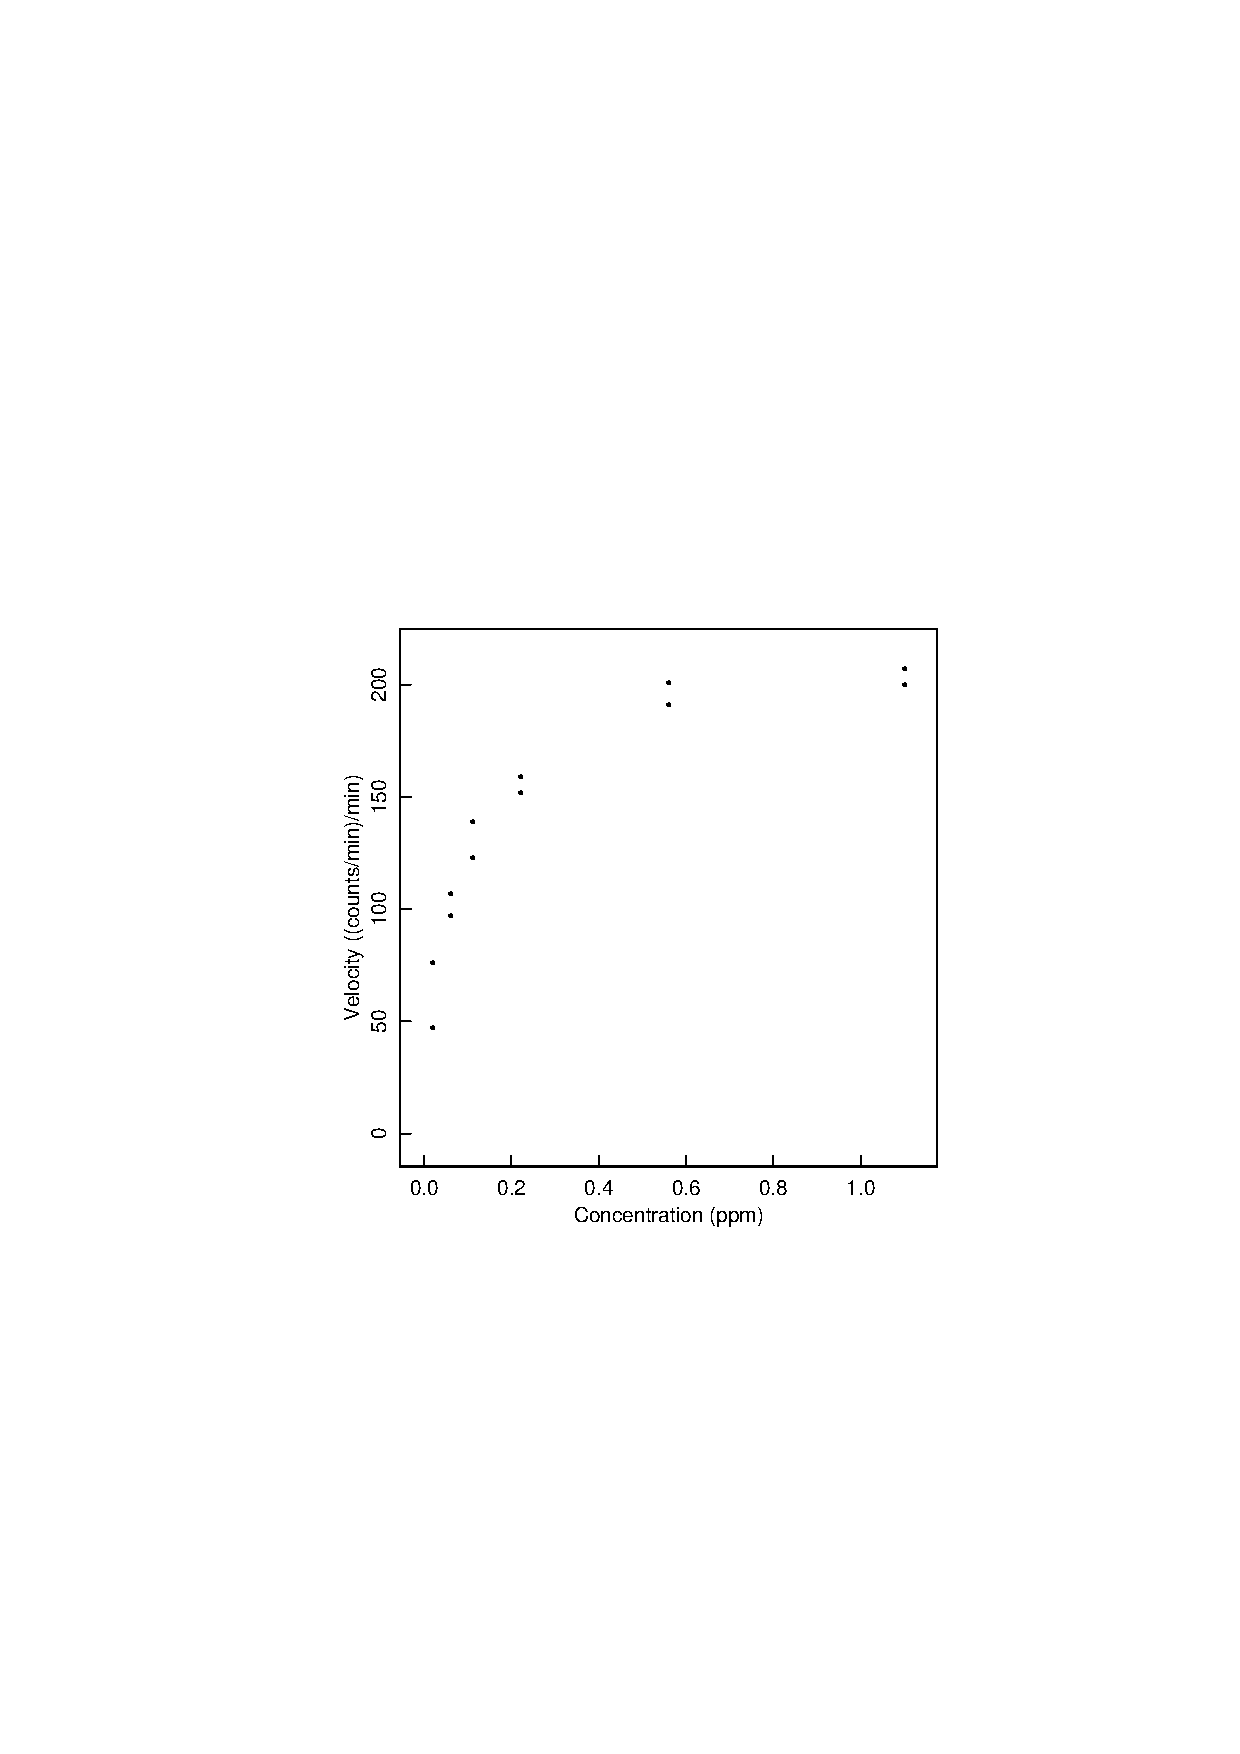
\includegraphics{2MICdata}%height=3in,width=!]{2MICdata}
  \caption{Plot of reaction velocity versus substrate concentration
    for the Puromycin data.}
  \label{fig:MICdata}
\end{figure}

Differentiating $f$ with respect to $\theta_1$ and $\theta_2$ gives
  \begin{eqnarray}\label{eqn:2.4}
    \frac{\partial f}{\partial\theta_1}&=&\frac{x}{\theta_2 + x}\\
    \frac{\partial f}{\partial \theta_2}&=&\frac{-\theta_1 x}{(\theta_2+ x )^2}\nonumber
  \end{eqnarray}
and since both these derivatives involve at least one of the
parameters, the model is recognized as nonlinear.
\end{example}

\subsection{Transformably Linear Models}
\index{nonlinear!model - transformably linear}
\index{transformably linear!model}

The Michaelis--Menten model (\ref{eqn:2.3}) can be transformed to a
linear model by expressing the reciprocal of the velocity as a
function of the reciprocal substrate concentration,
  \begin{eqnarray}\label{eqn:transmm}
    \frac{1}{f}&=&\frac{1}{\theta_1}+\frac{\theta_2}{\theta_1}\frac{1}{x}\\
    &=&\beta_1 + \beta_2 u\nonumber
  \end{eqnarray}

We call such models {\it transformably linear}.  Some authors use the
term ``intrinsically linear'',\index{nonlinear!"model-intrinsically
linear"}\index{"intrinsically linear"!model} but we reserve the term
``intrinsic'' for a special geometric property of nonlinear models, as
discussed in Chapter 7.  As will be seen in Chapter 3, transformably
linear models have some advantages in nonlinear regression because it
is easy to get starting values for some of the parameters.

It is important to understand, however, that a transformation of
the data involves a transformation of the disturbance
term too, which affects the assumptions on it.
Thus, if we
assume the model function (\ref{eqn:2.1}) with an additive, spherical
normal disturbance term is an appropriate representation of the
experimental situation, then these same assumptions will not be
appropriate for the transformed data.
Hence we should use
nonlinear regression on the original data, or else weighted least
squares on the transformed data.
Sometimes, of course, transforming a data set to induce constant variance
also produces a linear expectation function
in which case linear regression can be used on the transformed data.
\label{mic:2}
\begin{example}

Because there are replications in the Puromycin data set, it is
easy to see from
Figure \ref{fig:MICdata}
that the variance of the original data is constant,
and hence that nonlinear regression should be used to estimate
the parameters.
However, the reciprocal data, plotted in
Figure \ref{fig:MICinv}$a$,
  \begin{figure}
    \centerline{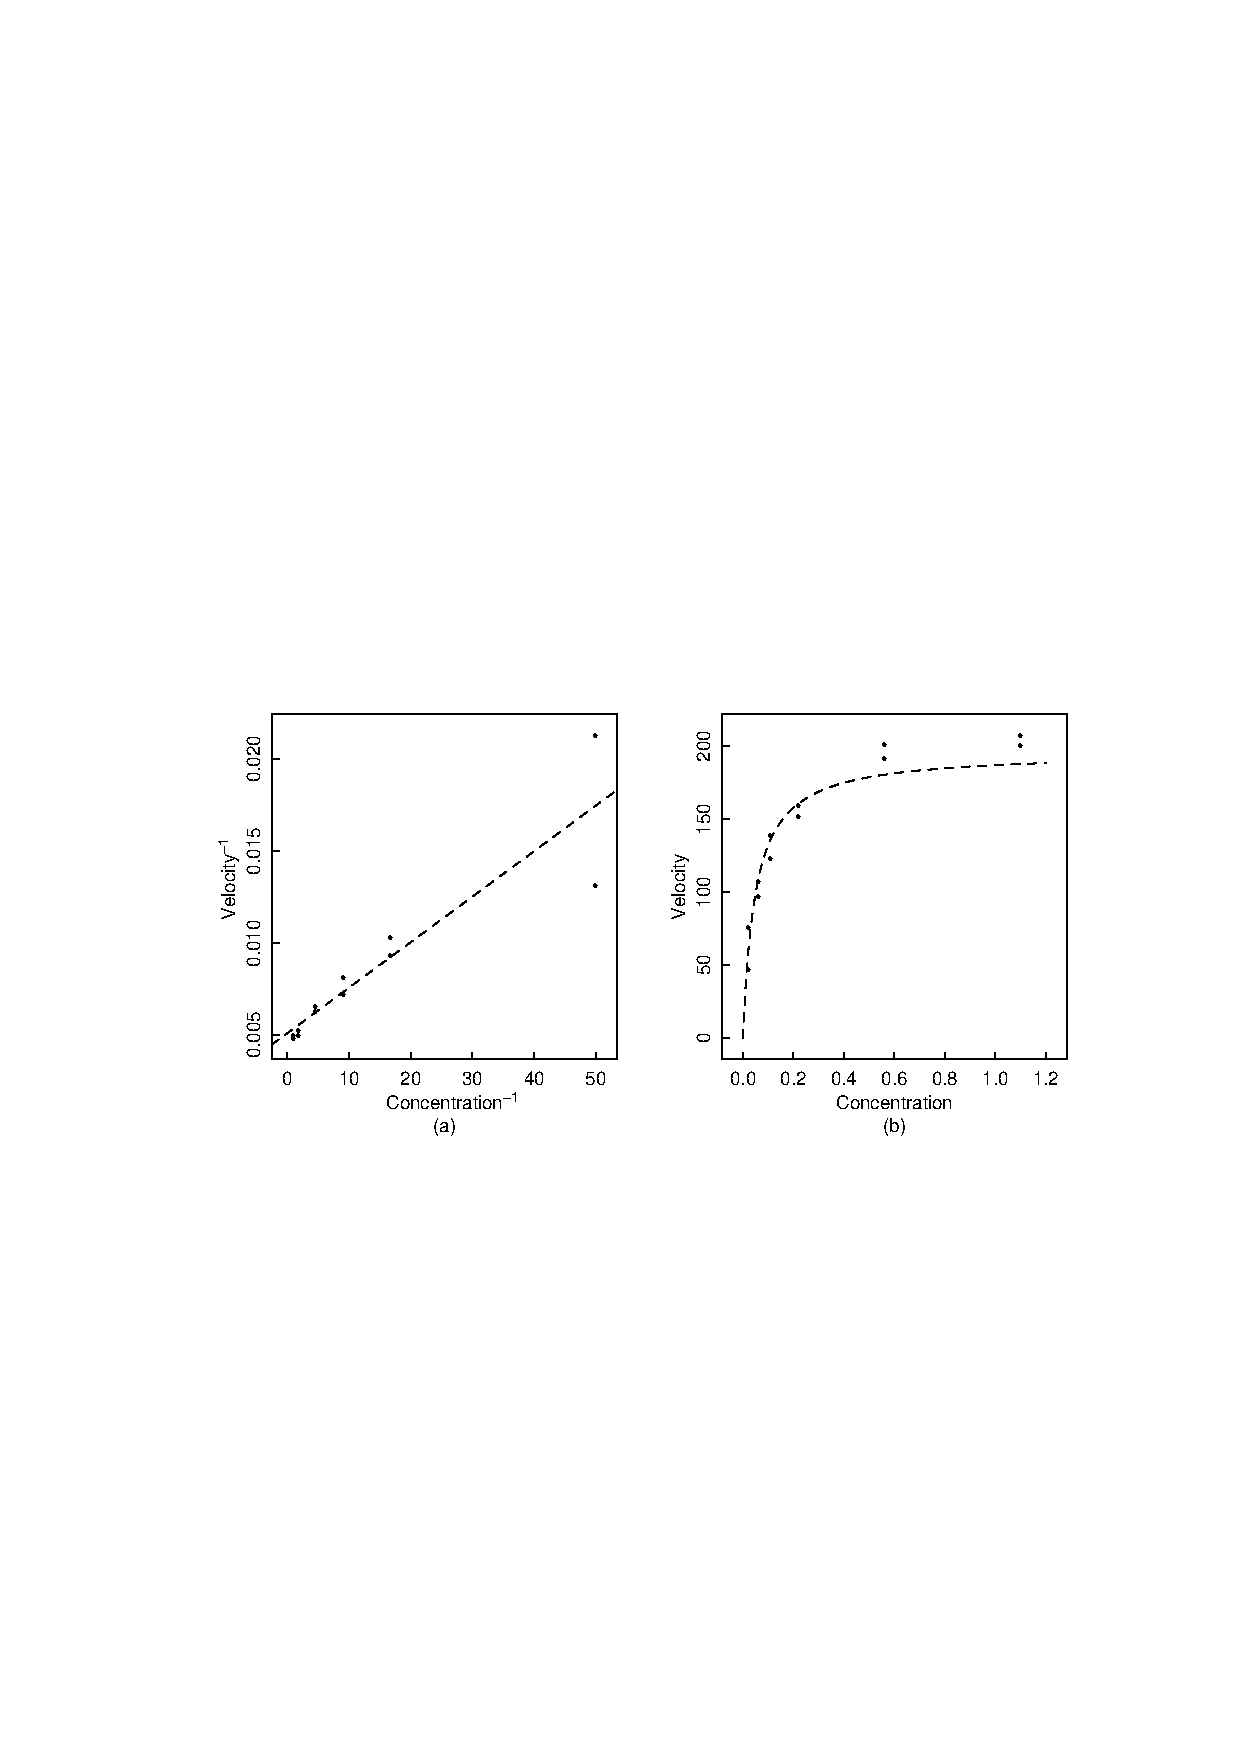
\includegraphics{2MICinv}}%,height=2.25in}}
    \caption[Puromycin Data on Inverse Scale]{\label{fig:MICinv}
    Plot of inverse velocity versus inverse substrate concentration for
    the Puromycin experiment with the linear regression line (dashed)
    in part $a$, and the corresponding fitted curve (dashed) in the original
    scale in part $b$.}
  \end{figure}
while showing a simple straight line relationship,
also show decidely nonconstant variance.
\index{variance!nonconstant}

If we use linear regression to fit the model (\ref{eqn:transmm}) to
these data, we obtain the estimates
  \begin{displaymath}
    \hat{\bbeta}=( 0.005107 ,  0.0002472 ) \trans
  \end{displaymath}
corresponding to
  \begin{displaymath}
    \hat{ \btheta}=( 195.8 ,  0.04841 ) \trans
  \end{displaymath}
The fitted curve is overlaid with the data in the original scale
in Figure \ref{fig:MICinv}$b$, where we see that the predicted
asymptote is too small.
Because the variance of the replicates has been distorted by
the transformation, the cases with low concentration (high
reciprocal concentration) dominate the determination of the
parameters and the curve does not fit the data well at high
concentrations.
\end{example}

This example demonstrates two important features.
First, it
emphasizes the value of replications, because without
\index{replication}
replications it may not be possible to detect either the constant
variance in the original data or the nonconstant variance in the
transformed data; and second, it shows that while transforming
can produce simple linear behavior, it also
affects the disturbances.
\subsection{Conditionally Linear Parameters}
\index{parameter!conditionally linear}

The Michaelis--Menten model is also an example of a model in which
there is a conditionally linear parameter, $\theta_1$.
It is {\it conditionally linear} because the
derivative of the expectation function with respect to
$\theta_1$ does not involve $\theta_1$.
We can therefore estimate $\theta_1$, conditional on $\theta_2$, by a
linear regression of velocity $x/(\theta_2+x)$.
Models with conditionally linear parameters enjoy some advantageous
properties, which can be exploited in nonlinear regression.

\subsection{The Geometry of the Expectation Surface}
\index{geometry}
\index{geometry!of the expectation surface}
\index{expectation surface!geometry}

The assumption of a spherical normal distribution for the disturbance
term $\bZ$ leads us to consider the Euclidean geometry of the
$N$-dimensional response space, because again we will be interested in
the least squares estimates $\hat{ \btheta}$ of the parameters.
The $N$-vectors $\boeta ( \btheta )$ define a $P$-dimensional surface
called the \emph{expectation surface} in the response space, and the
least
\index{response!space}
squares estimates correspond to the point on the expectation
surface\index{expectation surface},
  \begin{displaymath}
    \hat{\boeta}=\boeta(\hat{\btheta})
  \end{displaymath}
which is closest to $\by$.
That is, $\hat{\btheta}$ minimizes the residual sum of squares
  \begin{displaymath}
    S( \btheta ) = \norm \by - \boeta ( \btheta ) \norm^2
  \end{displaymath}
\label{rum:2}
\begin{example}

To illustrate the geometry of nonlinear models,
\index{geometry!of nonlinear models}
consider the two cases $t = 4$ and $t = 41$ for the Rumford data.
Under the assumption that Newton's law of cooling holds for these
data, the expected responses are
\begin{displaymath}
  \boeta ( \theta ) =
  \begin{bmatrix}
    60 + 70  e^{ - 4 \theta }\\60 + 70 e^{ - 41 \theta }
  \end{bmatrix}\quad
  \theta \ge 0
\end{displaymath}
Substituting values for $\theta$ in these equations and
plotting the points in a 2-dimensional response space
gives the 1-dimensional expectation surface (curve)
shown in Figure \ref{fig:RUM2esurf}.
  \begin{figure}
    \centerline{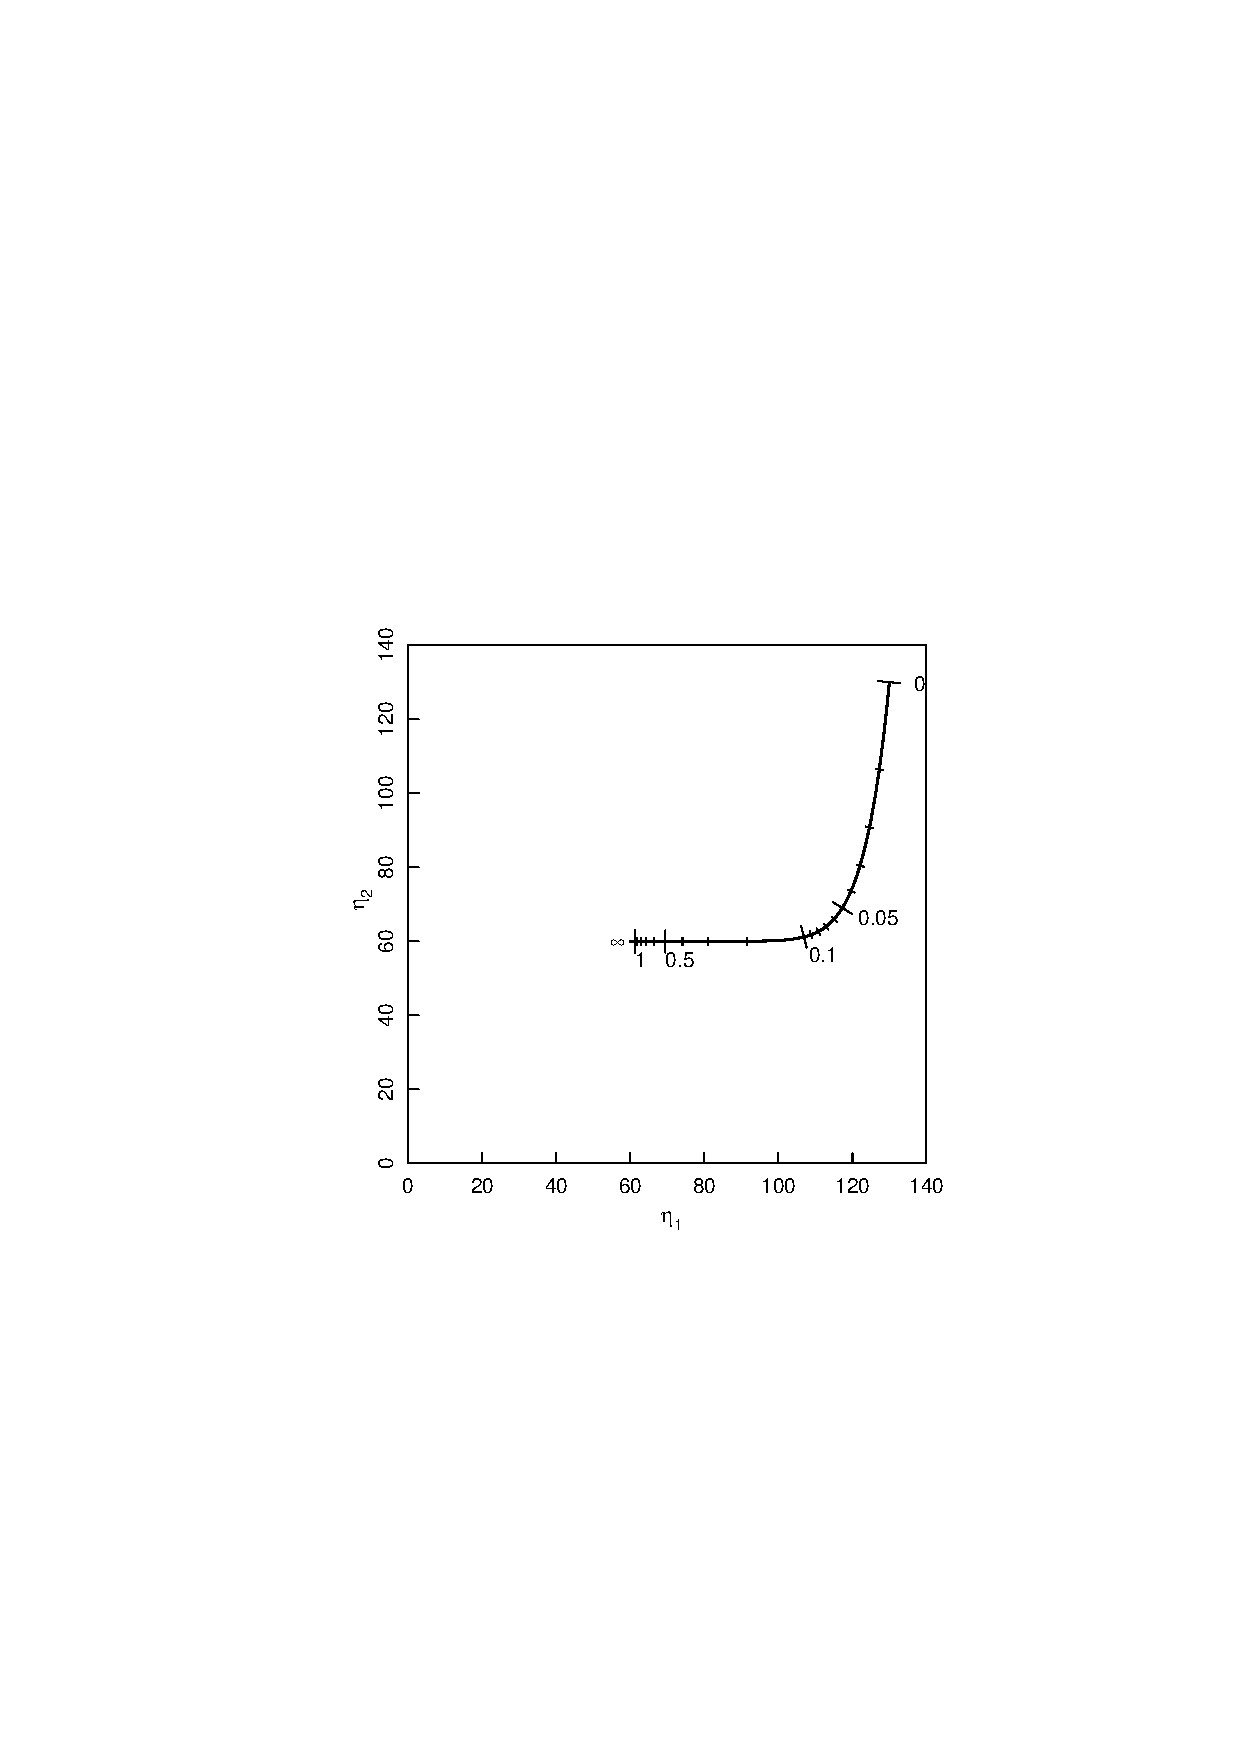
\includegraphics{2RUM2esurf}}%,height=3in}}
    \caption{\label{fig:RUM2esurf}
    Plot of the expectation surface (solid line) in the response space
    for the 2-case Rumford data.  The points corresponding to
    $\theta=0,0.01,0.02,\ldots,0.1,0.2,\ldots,1,\infty$ are marked.
    }
  \end{figure}

Note that the expectation surface is {\it curved} and of {\it finite
extent}, which is in contrast to the linear model in which 
the expectation surface is a plane of infinite extent.
Note, too, that points with equal spacing on the parameter line
($\theta$) map to points with unequal spacing on the expectation
surface.
\end{example}
\label{mic:3}
\begin{example}

As another example, consider the three cases from
Example Puromycin \ref{mic:1}: $x = 1.10$, $x = 0.56$, and
$x = 0.22$.
Under the assumption
that the expectation function (\ref{eqn:2.3}) is the correct one, the
expected responses for these substrate values are
\begin{displaymath}
  \boeta ( \btheta ) =
  \begin{bmatrix}
    \frac{\theta_1(1.10)}{\theta_2+1.10}\\
    \frac{\theta_1(0.56)}{\theta_2+0.56}\\
    \frac{\theta_1(0.22)}{\theta_2+0.22}\\
  \end{bmatrix}
  \quad\theta_1 , \theta_2 \ge 0
  \end{displaymath}
and so we can plot the expectation surface by substituting values
for $\btheta$ in these equations.
A portion of the
2-dimensional expectation surface for these $x$ values is
\index{expectation surface}
shown in
Figure \ref{fig:MICesurf}.
  \begin{figure}
    \centerline{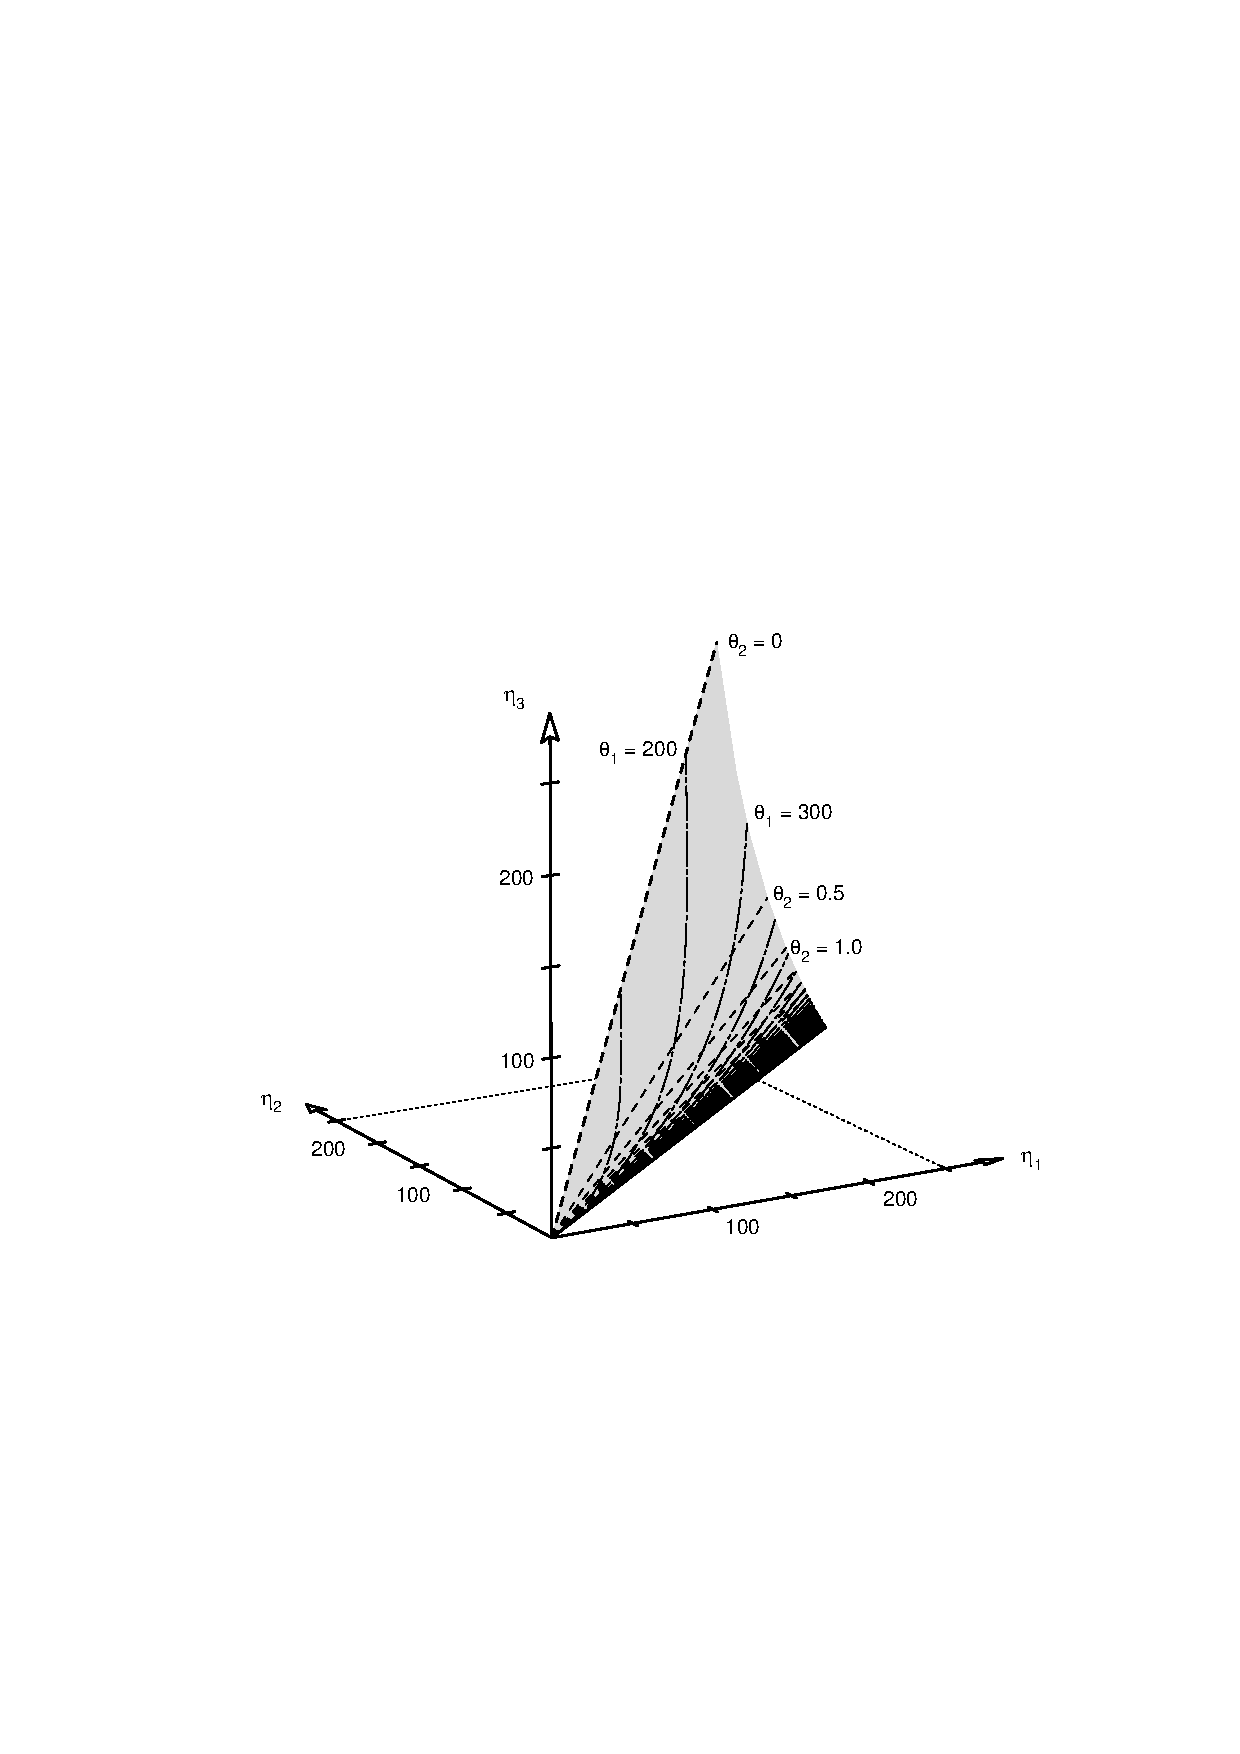
\includegraphics{2MICesurf}}%,height=4.5in}}
    \caption[3-case Puromycin example]{\label{fig:MICesurf}
    Expectation surface for the 3-case Puromycin example.
    We show a portion of the expectation surface (shaded) in the
    expectation space with $\theta_1$ parameter lines (dashed) and
    $\theta_2$ parameter lines (dot--dashed).
    }
  \end{figure}
Again, in contrast to the linear model,
this expectation surface is not an infinite plane, and in
general, straight lines in the parameter plane do not map to
straight lines on the expectation surface.
It is also seen that unit squares in
the parameter plane map to irregularly shaped areas on
\index{parameter!plane}
the expectation surface and that the sizes of these areas
vary.
Thus, the Jacobian determinant is not
\index{Jacobian!determinant}
\index{determinant!Jacobian}
constant, which
can be seen analytically, of course, because the
derivatives (\ref{eqn:2.4}) depend on $\btheta$.

For this model, there are straight lines on the expectation
surface in Figure \ref{fig:MICesurf} corresponding to the $\theta_1$
parameter lines (lines with $\theta_2$ held constant),
\index{parameter!line on expectation surface}
reflecting the fact that $\theta_1$ is conditionally linear.
However, the $\theta_1$ parameter lines are neither parallel
nor equispaced.
The $\theta_2$ lines are not straight, parallel, or equispaced.
\end{example}

As can be seen from these examples, for nonlinear models with
$P$ parameters, it is generally true that:
\begin{enumerate}

  \item the expectation surface, $\boeta ( \btheta )$, is a
        $P$-dimensional {\it curved surface} in the $N$-dimensional
        response space;

  \item parameter {\it lines} in the parameter space map to {\it
        curves} on the curved expectation surface; 

  \item the {\it Jacobian determinant}, which measures how large
        unit areas in $\btheta$ become in $\boeta ( \btheta )$, is
        {\it not constant}.

\end{enumerate}

We explore these interesting and important aspects of the
expectation surface later, but first we discuss how to obtain
the least squares estimates $\hat{ \btheta}$ for the parameters $\btheta$.
Nonlinear least squares estimation from the point of view
of sum of squares contours is given in Section 2.4.

\section{Determining the Least Squares Estimates}

The problem of finding the least squares estimates can be stated
\index{least squares!estimates for nonlinear model}
\index{least squares!geometry}
very simply geometrically---given a data vector
$\by$, an expectation function $f  ( \bx_n ,\btheta )$,
and a set of design vectors $\bx_n$, $n = 1 ,\ldots, N$
\par\vspace{1.0\baselineskip}
%.ln
(1)find the point $ \hat{ \boeta} $ on the expectation surface
which is closest to $\by$, and then
%.ln
(2)determine the parameter vector $\hat{ \btheta}$ which corresponds to the
point $ \hat{ \boeta} $.


For a linear model, step (1) is straightforward because the
expectation surface is a plane of infinite extent, and we
may write down an explicit expression for the point on that
plane which is closest to $\by$,
  \begin{displaymath}
    \hat{ \boeta} = \bQ_1 {\bQ_1 \trans} \by
  \end{displaymath}
For a linear model, step (2) is also straightforward because the
$P$-dimensional parameter plane maps linearly and invertibly to
the expectation plane, so once we know where we are on one plane we
can easily find the corresponding point on the other.  Thus
  \begin{displaymath}
    \hat{ \bbeta} = {\bR_1^{-1}} { \bQ_1 \trans} \hat{ \boeta}
  \end{displaymath}

In the nonlinear case, however, the two steps are very difficult: the
first because the expectation surface is curved and often of finite
extent (or, at least, has edges) so that it is difficult even to find
$\hat{ \boeta}$, and the second because we can map points easily only in one
direction---from the parameter plane to the expectation surface.
That is, even if we know $\hat{ \boeta}$, it is extremely
difficult to determine the parameter plane coordinates $\hat{ \btheta}$
corresponding to that point.
To overcome these difficulties, we use iterative methods to
\index{iteration}
determine the least squares estimates.
\subsection{The Gauss--Newton Method 2 2 1}
\index{Gauss-Newton!method}

An approach suggested by Gauss is to use a linear approximation
to the expectation function to iteratively improve
an initial guess $\btheta^0$
for $\btheta$ and keep improving the
estimates until there is no change.
That is, we expand the expectation function
\index{expectation function!linear approximation to}
\index{linear approximation!to expectation function}
$f  ( \bx_n ,\btheta )$ in a first order Taylor
series about $\btheta^0$ as
  \begin{displaymath}
    f(\bx_n,\btheta)\approx f(\bx_n,\btheta^0)+
    \mbox{\rm v}_{n1} ( \theta_1 - \theta_1^0 ) +
    \mbox{\rm v}_{n2} ( \theta_2 - \theta_2^0 ) + \ldots +
    \mbox{\rm v}_{nP} ( \theta_P - \theta_P^0 )
  \end{displaymath}
where
  \begin{displaymath}
    \mbox{\rm v}_{np}=\left. \frac{\partial f  ( \bx_n ,\btheta )}{
    \partial \theta_p} \right|_{ \theta^0} p = 1, 2 ,\ldots, P
  \end{displaymath}
Incorporating all $N$ cases, we write
  \begin{equation}\label{eqn:2.5}
  \boeta ( \btheta ) \approx
  \boeta ( \btheta^0 ) + \bV^0 ( \btheta - \btheta^0 )
  \end{equation}
where $\bV^0$ is the $N \times P$ derivative matrix with elements
\index{derivative matrix}
\index{matrix!derivative}
$\mbox{\rm v}_{np}$.
This is equivalent to approximating the residuals,
$\bz ( \btheta )   = \by - \boeta ( \btheta )$, by
\index{residual}
  \begin{equation}\label{eqn:2.5a}
  \bz ( \btheta )\approx \by - [ \boeta ( \btheta^0 ) + \bV^0 \bdelta ]
  =\bz^0-\bV^0 \bdelta
  \end{equation}
where $\bz^0=\by-\boeta(\btheta^0)$ and $\bdelta=\btheta-\btheta^0$.

We then calculate the \emph{Gauss increment}\index{Gauss increment}
$\bdelta^0$ to minimize the approximate residual sum of squares
$\norm \bz^0 - \bV^0 \bdelta \norm^2$, using
  \begin{eqnarray*}
    \bV^0&=&\bQ \bR = \bQ_1 \bR_1\hfill\mbox{\rm [cf.(1.19)]}\\
    \bw_1&=&\bQ_1 \trans \bz^0\hfill\mbox{\rm [cf.(1.21)]}\\
    \hat{ \boeta}^1&=&\bQ_1 \bw_1\hfill\mbox{\rm [cf.(1.23)]}
  \end{eqnarray*}
and so
  \begin{displaymath}
    \bR_1 \bdelta^0 = \bw_1\hfill\mbox{\rm [cf.(1.24)]}
  \end{displaymath}
The point
  \begin{displaymath}
    \hat{\boeta}^1=\boeta(\btheta^1)=\boeta(\btheta^0+\bdelta^0)
  \end{displaymath}
should now be closer to $\by$ than $\boeta(\btheta^0)$, and so we move
to this better parameter value $\btheta^1=\btheta^0+\bdelta^0$
and perform another iteration by calculating new residuals
$\bz^1 = \by - \boeta ( \btheta^1 )$, a new derivative
matrix $\bV^1$, and a new increment.
This process is repeated until convergence\index{ convergence} is
obtained, that is, until the increment is so small that there is no
useful change in the elements of the parameter vector.

\begin{example}\label{mic:4}

To illustrate these calculations, consider the data from Example
Puromycin \ref{mic:1}, with the starting estimates
$\btheta^0=(205,0.08)\trans$.
The data, along with the fitted values, residuals, and derivatives
evaluated at $\btheta^0$, are shown in Table \ref{tbl:2.1}.
\begin{table}
  \caption{\label{tbl:2.1} Residuals and derivatives for Puromycin
  data at $\theta=(205,0.08)\trans$.}
  \begin{center}
    \begin{tabular}{l c c c c c c}\hline
      \multicolumn{1}{c}{$n$} & \multicolumn{1}{c}{$x_{n}$} &
      \multicolumn{1}{c}{$y_{n}$} & \multicolumn{1}{c}{$\eta_n^0$} &
      {$z_n^0$} & \multicolumn{1}{c}{${\rm v}_{n1}^0$} & {$ v_{n2}^0$}\\
      \hline 1&0.02&76&41.00&35.00&0.2000&--410.00\\
      2&0.02&47&41.00&6.00&0.2000&--410.00\\
      3&0.06&97&87.86&9.14&0.4286&--627.55\\
      4&0.06&107&87.86&19.14&0.4286&--627.55\\
      5&0.11&123&118.68&4.32&0.5789&--624.65\\
      6&0.11&139&118.68&20.32&0.5789&--624.65\\
      7&0.22&159&150.33&8.67&0.7333&--501.11\\
      8&0.22&152&150.33&1.67&0.7333&--501.11\\
      9&0.56&191&179.38&11.62&0.8750&--280.27\\
      10&0.56&201&179.38&21.62&0.8750&--280.27\\
      11&1.10&207&191.10&15.90&0.9322&--161.95\\
      12&1.10&200&191.10&8.90&0.9322&--161.95\\ \hline
    \end{tabular}
  \end{center}
\end{table}

Collecting these derivatives into the derivative matrix $\bV^0$, we then
perform a \emph{QR} decomposition, from which we generate
$\bw_1=\bQ_1 \trans \bz^0$
and then solve for $\bdelta^0$ using
$\bR_1 \bdelta^0=\bw_1$.
In this case,
$\bdelta^0=(8.03,-0.017)\trans$
and the sum of squares at
$\btheta^1=\btheta^0 +\bdelta^0$
is $S( \btheta^1 )=1206$, which is much
smaller than $S( \btheta^0 ) = 3155$.  We therefore move to
$\btheta^1 = (213.03,  0.063) \trans$ and perform another
iteration.
\end{example}
\label{bod:BODdata}
\begin{example}

As a second example, we consider data on biochemical oxygen demand
(BOD) from \citeasnoun{mars:1967}, reproduced in
%\glossary{ Marske, D.}
Appendix~\ref{atbl:bod}.  The data are plotted in
Figure \ref{fig:BODdata}.
\begin{figure}
  \centerline{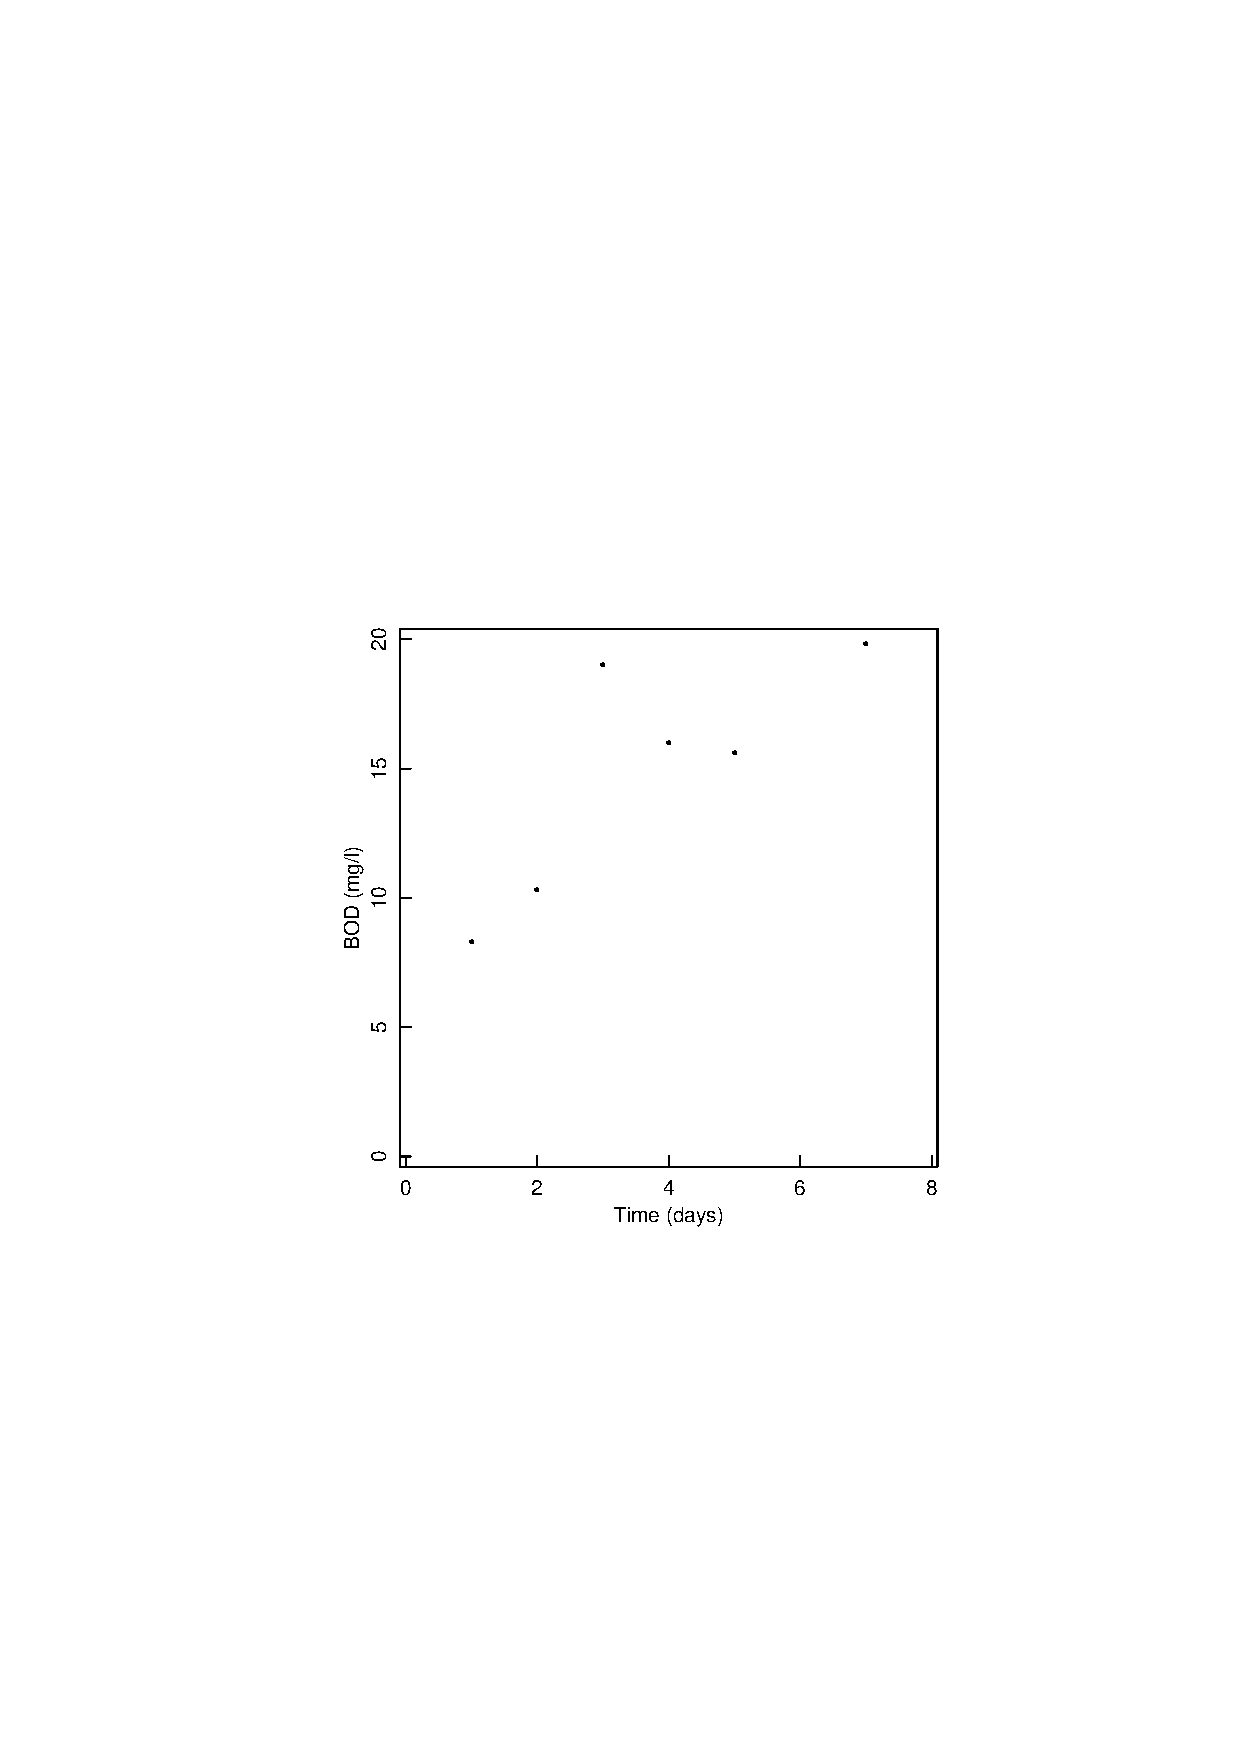
\includegraphics{2BODdata}}%,height=3in}}
  \caption{\label{fig:BODdata}
  Plot of BOD versus time}
\end{figure}
For these data, the model
\begin{equation}\label{eqn:2.6a}
  f(x,\btheta)=\theta_1(1-e^{\theta_2 x})
\end{equation}
is considered appropriate.

Using the starting estimates $\btheta^0=(20,0.24)\trans$,
for which $S ( \btheta^0 )=128.2$, produces an increment to
$\btheta^1 = ( 13.61 ,  0.52 ) \trans$ with $S ( \btheta^1 )
= 145.2$.  In this case, the sum of squares has increased and so
we must modify the increment as discussed below.
\end{example}

\subsection*{Step Factor}
\index{step factor}

As seen in the last example, the Gauss--Newton increment can produce
an \emph{increase}
in the sum of squares when the requested increment
extends beyond the region where the linear approximation
is valid.  Even in these circumstances, however, the linear
approximation will be a close approximation to the actual surface for
a sufficiently small region around $\boeta ( \btheta^0 )$.
Thus a small step in the direction $\bdelta^0$ should produce
a decrease in the
sum of squares.
We therefore introduce a \emph{step factor}
$\lambda$,
and calculate
  \begin{displaymath}
    \btheta^1 = \btheta^0 + \lambda \bdelta^0
  \end{displaymath}
where $\lambda$ is chosen to ensure that
  \begin{equation}\label{eqn:stepfactor}
  S ( \btheta^1 ) < S ( \btheta^0 )
  \end{equation}
A common method of selecting $\lambda$ is to start with $\lambda=1$
and halve it until (\ref{eqn:stepfactor}) is satisfied.  This
modification to the Gauss--Newton algorithm was suggested in
\citeasnoun{box:1960}%\glossary{ Box, G.E.P.} and
\citeasnoun{hart:1961}%\glossary{ Hartley, H.O.}. 

\begin{example}\label{bod:stephalf}
For the data and starting estimates in Example BOD \ref{bod:BODdata},
the value $\lambda = 0.5$ gave a reduced sum of squares, 94.2, at
$\btheta=(16.80,0.38)\trans$. 
\end{example}

Pseudocode for the Gauss--Newton algorithm for nonlinear least
squares is given in Appendix 3, Section A3.1, together with
implementations in GAUSS, S, and SAS/IML.

\subsection{The Geometry of Nonlinear Least Squares}
\index{geometry!of nonlinear least squares}
\index{least squares!geometry of nonlinear}

Geometrically a Gauss--Newton iteration consists of:
  \begin{enumerate}
    \item approximating $\boeta ( \btheta )$ by a Taylor series
          expansion at $\boeta^0 = \boeta ( \btheta^0 )$,
    \item generating the residual vector $\bz^0 = \by - \boeta^0$,
    \item projecting the residual $\bz^0$ onto the tangent plane
          \index{tangent plane}
          to give $\hat{ \boeta}^1$,
    \item mapping $\hat{ \boeta}^1$ through the linear coordinate
          system to produce the increment $\bdelta^0$, and finally
    \item moving to $\boeta ( \btheta^0 + \lambda  \bdelta^0 )$.
  \end{enumerate}

The first step actually involves two distinct approximations:
  \begin{enumerate}
    \item the \emph{planar} assumption, in which we approximate the
          expectation surface
          \index{assumptions!planar}
          \index{planar assumption}
          $\boeta ( \btheta )$ near $\boeta ( \btheta^0 )$ by its
          tangent plane at $\boeta ( \btheta^0 )$, and
    \item the \emph{uniform coordinate} assumption, in which we
          \index{assumptions!uniform coordinate}
          \index{uniform coordinate!assumption}
          impose a linear coordinate system $\bV(\btheta-\btheta^0)$
          on the approximating tangent plane.
  \end{enumerate}

We give geometrical interpretations of these steps and
assumptions in the following examples.

\begin{example}\label{rum:3}
For the 2-case Rumford data set of Example Rumford \ref{rum:2},
we plot $\by$ and a portion of the expectation surface
in Figure \ref{fig:RUM2inc}.
  \begin{figure}
    \centerline{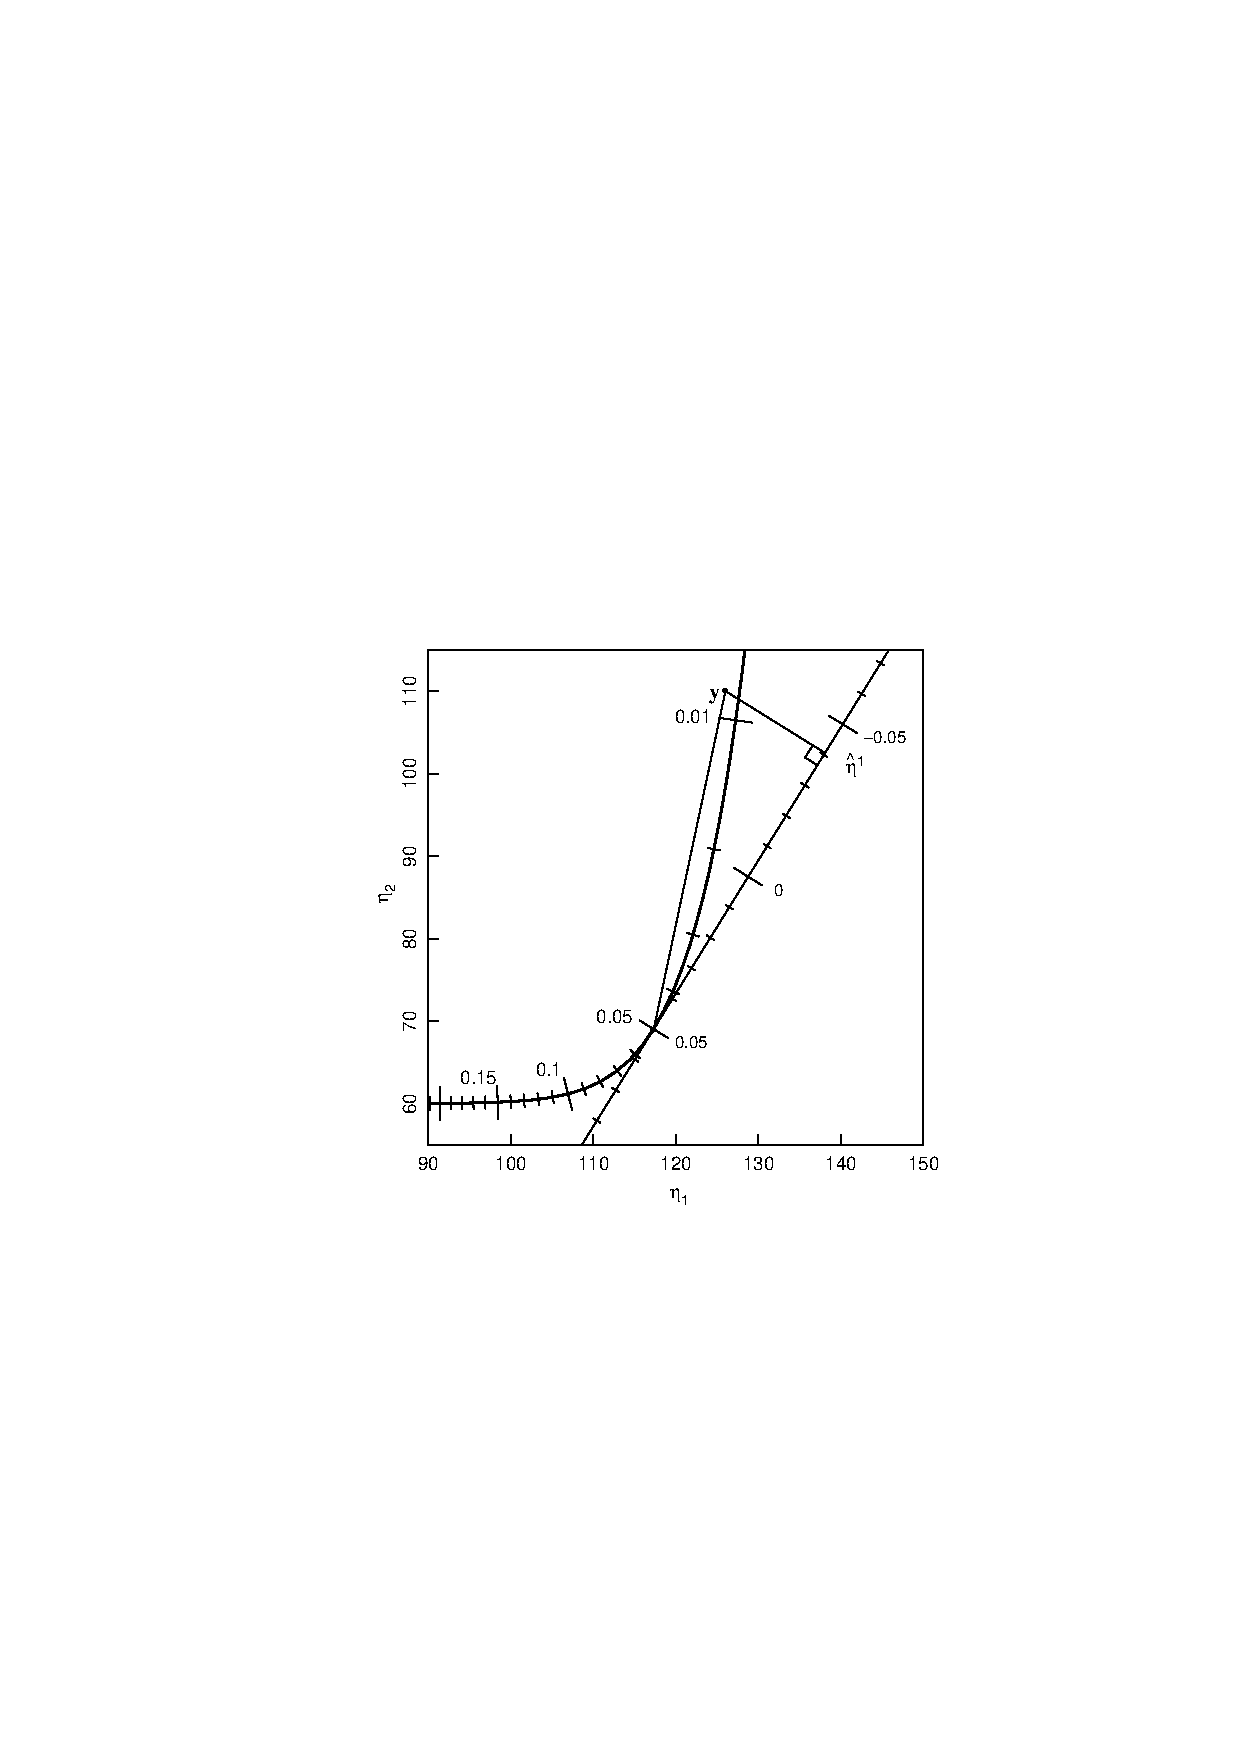
\includegraphics{2RUM2inc}}%,height=3in}}
    \caption[Gauss-Newton increment for the Rumford data]{
    \label{fig:RUM2inc}
    A geometric interpretation of calculation of the Gauss--Newton
    increment using the 2-case Rumford data.
    A portion of the expectation surface (heavy solid line) is shown in
    the response space together with the observed response $\by$.
    Also shown is the projection $\hat{ \boeta}^1$ of
    $\by-\boeta ( 0.05 )$ onto the tangent plane at $\boeta ( 0.05 )$
    (solid line).
    The tick marks indicate true positions on the expectation surface and
    linear approximation positions on the tangent plane.
    }
  \end{figure}
The expectation surface is a curved line, and the points
corresponding to $\theta = 0.01,0.02 ,\ldots, 0.2$ are unevenly
spaced.

For the initial estimate $\theta^0 = 0.05$, a
Gauss--Newton iteration involves the linear approximation
\begin{displaymath}
  \boeta ( \theta ) \approx \boeta^0 + \bv  \delta
\end{displaymath}
where $\delta = ( \theta - 0.05 )$, $\boeta^0$ is the expectation
vector at $\theta = 0.05$,
\begin{displaymath}
  \begin{bmatrix}60 + 70 e^{ -4 \theta }\\60 + 70 e^{ -41 \theta }\end{bmatrix}
  \begin{bmatrix} 117.31 \\ 69.01 \end{bmatrix}
\end{displaymath}
and $\bv$ is the derivative vector at $\theta = 0.05$,
\begin{displaymath}
  \bv =  \begin{bmatrix}- 70(4) e^{ -4 \theta }\\-70(41) e^{ -41 \theta }\end{bmatrix}
  = \begin{bmatrix}-229.25 \\ -369.47 \end{bmatrix}
\end{displaymath}
The Taylor series approximation, consisting of the tangent plane and
the linear coordinate system, is shown as a solid line in
Figure \ref{fig:RUM2inc}.
This replaces the curved expectation surface with the nonlinear
parameter coordinates by a linear surface with a uniform coordinate
system on it.

Next we use linear least squares to obtain the point
$\hat{ \boeta}^1$ on the tangent line which is closest to $\by$.
We then calculate the \emph{apparent} parameter increment
$\delta^0$ corresponding to $\hat{ \boeta}^1$ and from this
obtain $\theta^1 = \theta^0 + \delta^0$.
For this example,
\begin{displaymath}
  \bz^0 =
  \begin{bmatrix}126 \\ 110 \end{bmatrix}
  - \begin{bmatrix} 117.31 \\ 69.01 \end{bmatrix}
  =  \begin{bmatrix} 8.69 \\ 40.99\end{bmatrix}
\end{displaymath}
so
$\hat{ \boeta}^1 = ( 138.1 ,  102.5 ) \trans$,
$\delta^0 = -0.091$, and
$\theta^1=0.05-0.091=-0.041$.

It is clear that the linear approximation increment is too large,
since $\theta^1 = -0.041$, whereas we can see from the points on
the expectation surface that $\hat{ \theta}$ is near 0.01.
We must therefore use a step factor to reduce the increment before
proceeding.
\end{example}
\par\vspace{-6.0pt}
\label{mic:5}
\begin{example}

For a two parameter example, we consider the data and the
starting values from Example Puromycin \ref{mic:4}.
Since the response space is 12-dimensional, we cannot picture it
directly, but we can represent the salient features in the
3-dimensional space spanned by the tangent plane and the
residual vector.
\begin{figure}
  \centerline{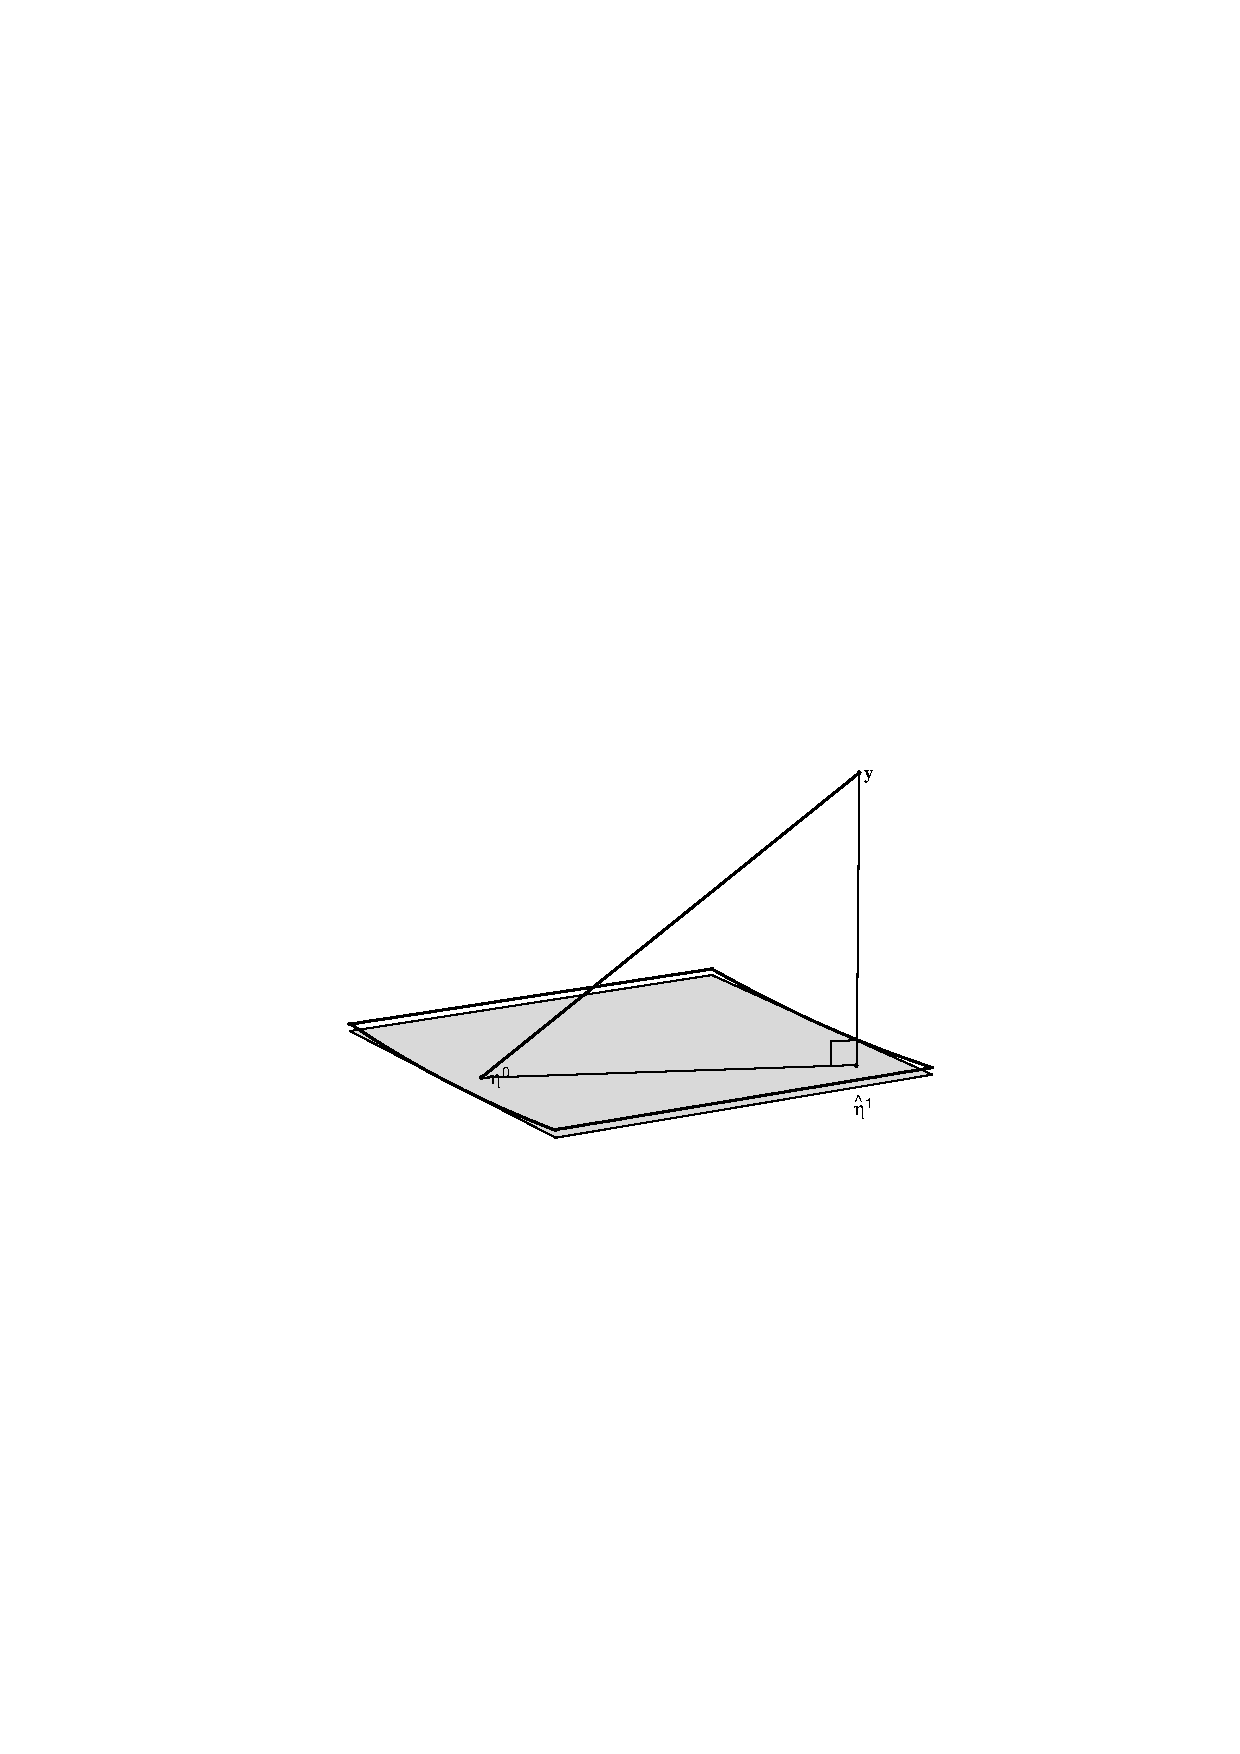
\includegraphics{2MICintrinsic}}%,height=3in}}
  \caption[Gauss-Newton increment for Puromycin data]{
    \label{fig:MICintrinsic}
    A geometric interpretation of calculation of the Gauss--Newton
    increment using the full Puromycin data set.
    We show the projection of a portion of the expectation surface into the
    subspace spanned by the tangent plane at $\boeta^0$
    (shaded) and the residual vector $\by-\boeta^0$.
    The region on the expectation surface is bordered by
    the heavy solid lines.
    Also shown is the projection $\hat{ \boeta}^1$ of the residual
    vector onto the tangent plane.
  }
\end{figure}
We do this in Figure \ref{fig:MICintrinsic}, where we show a portion
of the curved expectation surface, the residual vector, and the
approximating tangent plane.
\index{tangent plane!approximation to expectation surface}
It can be seen that the expectation surface is
only slightly curved, and so is well approximated by the tangent
plane.
\begin{figure}
  \centerline{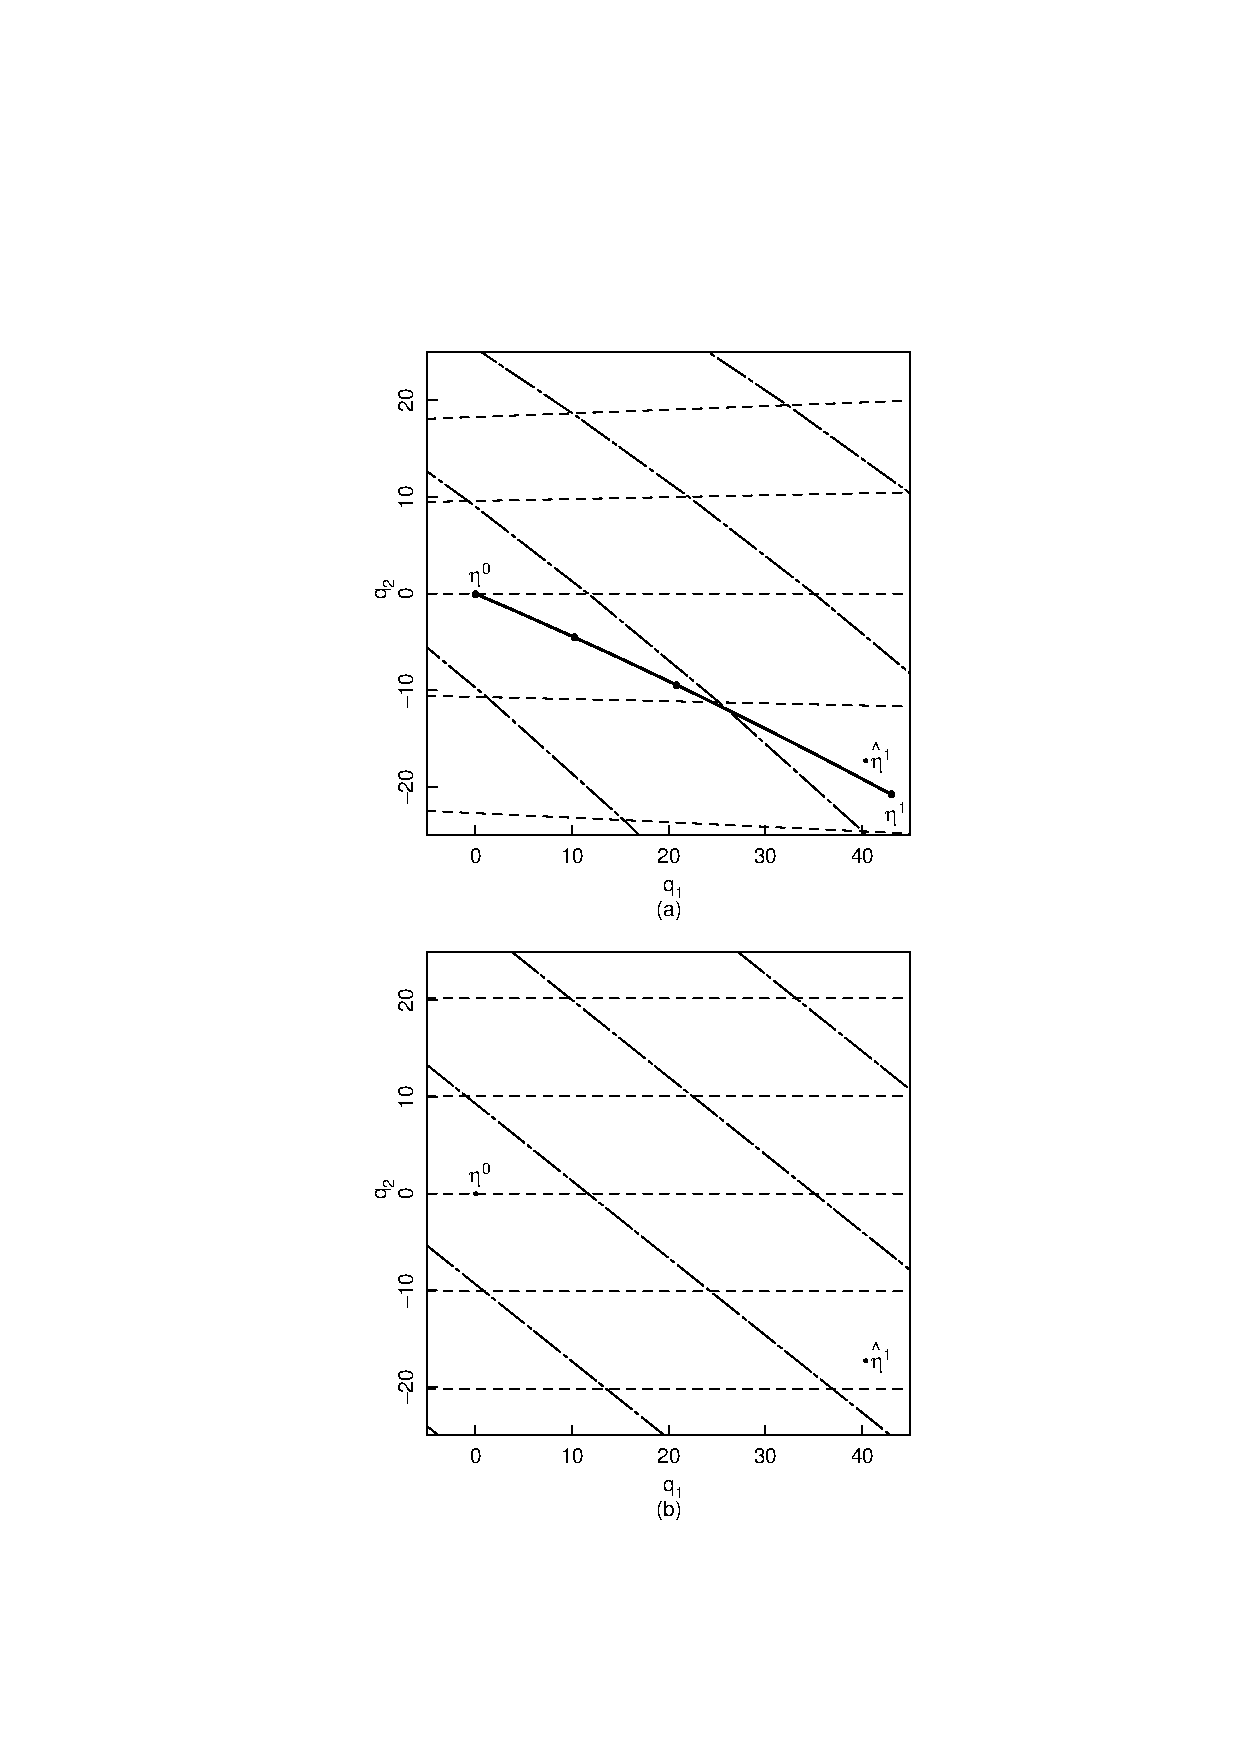
\includegraphics{2MICpeffects}}%,width=\textwidth}}
  \caption[Gauss-Newton increment for Puromycin data]{
    \label{fig:MICpeffects}
    A geometric interpretation of calculation of the Gauss--Newton
    increment using the full Puromycin data set (continued).
    The points $\boeta^0$ and $\hat{ \boeta}^1$ are shown in the
    tangent planes together with the parameter curves in part $a$ and the
    linear approximation parameter lines in part $b$.
    In part $a$ we also show the projection $\boeta^1$ of the point
    $\boeta(\btheta^0+\bdelta^0 )$.
    The curve (heavy solid line) joining $\boeta^0$ to $\boeta^1$ is
    the projection of $\boeta ( \btheta^0+\lambda\bdelta^0 )$ for
    $0\le\lambda\le1$.
    The points corresponding to $\lambda = 0.25$ and $0.5$ are marked.
  }
\end{figure}

In Figure \ref{fig:MICpeffects}$a$ we show the parameter curves for
\index{parameter!curve}
$\theta_1 = 200,210,220,230$ and
$\theta_2 = 0.06,0.07 ,\ldots,0.1$ projected onto the tangent plane,
and in Figure \ref{fig:MICpeffects}$b$ the corresponding linear
approximation lines on the tangent plane.
\index{parameter!linear approximation line to curve}
It can be seen that the linear approximation lines
match the true parameter curves very well.
Also shown on the tangent planes are the points $\boeta^0$
and $\hat{ \boeta}^1$ and in Figure \ref{fig:MICpeffects}$a$ the
projection of the curve
$\boeta ( \btheta^0 + \lambda  \bdelta^0 )$ for
$0 \le \lambda \le 1$.
The points corresponding to $\lambda = 0.25, 0.5$, and
$1$ ($\boeta^1$) are marked.

Because the planar and uniform coordinate assumptions are both
\index{planar assumption}
\index{uniform coordinate!assumption}
valid, the points $\hat{ \boeta}^1$ and $\boeta^1$ are close
together and are much closer to $\by$ than $\boeta^0$.
In this case, a full step ($\lambda = 1$) can be taken resulting
in a decrease in the sum of squares as shown in Example
Puromycin \ref{mic:4}.
\end{example}
\par\vspace{5.0pt}
\label{bod:1}
\begin{example}

As a second two-parameter example, we consider the data and
starting values from Example BOD \ref{bod:BODdata}.
  \begin{figure}
    \centerline{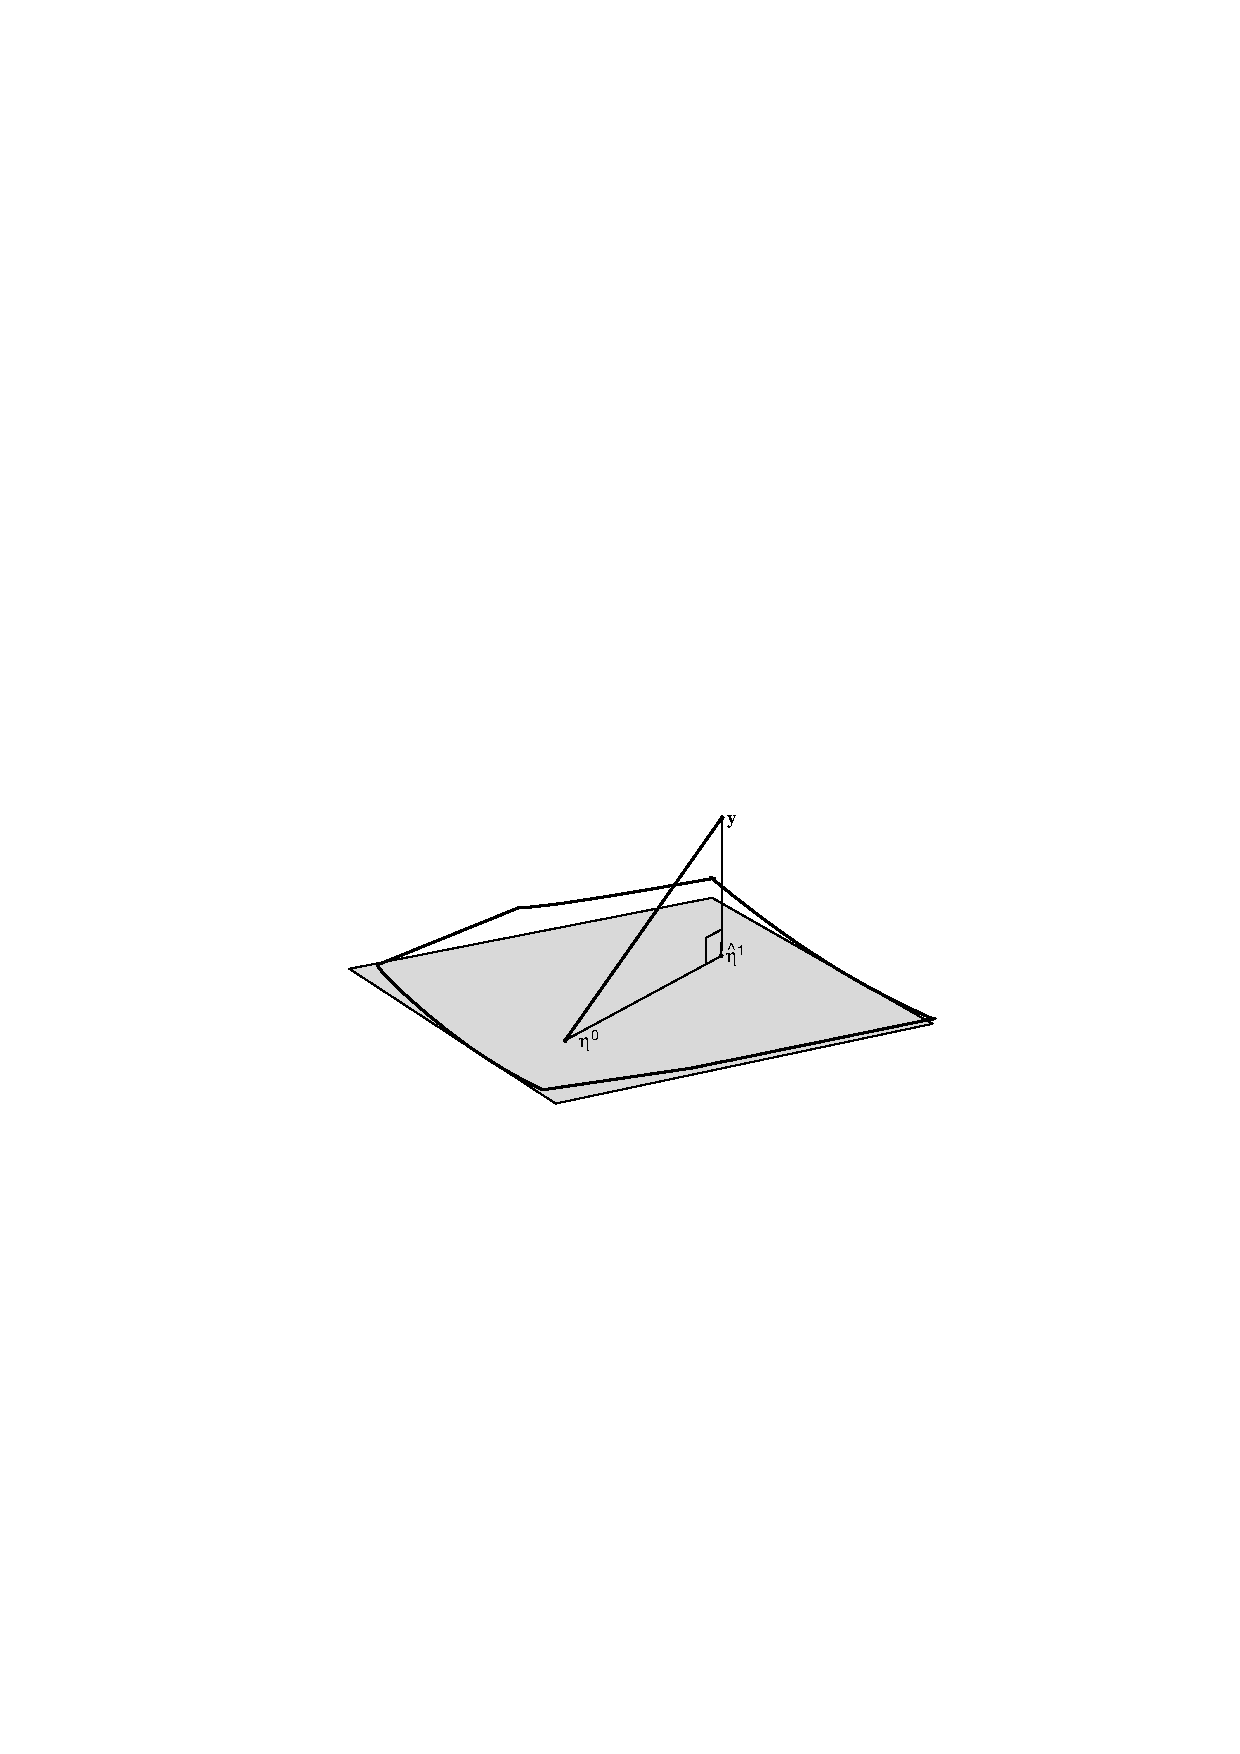
\includegraphics{2BODintrinsic}}%,height=3in}}
    \caption[Gauss-Newton increment for BOD data]{
    \label{fig:BODintrinsic}
    A geometric interpretation of calculation of the Gauss--Newton
    increment using the BOD data set.
    We show the projection of a portion of the expectation surface into the
    subspace spanned by the tangent plane at $\boeta^0$
    (shaded) and the residual vector $\by-\boeta^0$.
    The region on the expectation surface is bordered by
    the heavy solid lines.
    Also shown is the projection $\hat{ \boeta}^1$ of the residual
    vector onto the tangent plane.
    }
  \end{figure}
In Figure \ref{fig:BODintrinsic} we show a
portion of the curved expectation surface,
the residual vector, and the approximating tangent plane
in the space spanned by the tangent plane and the residual vector.
It can be seen that
the expectation surface is moderately curved, but is still apparently
well approximated by the tangent plane.
\index{tangent plane!approximation to expectation surface}
\index{planar assumption}
In this example, the edge of the finite expectation surface is shown as
the angled solid line along the top edge of the surface.
  \begin{figure}
    \centerline{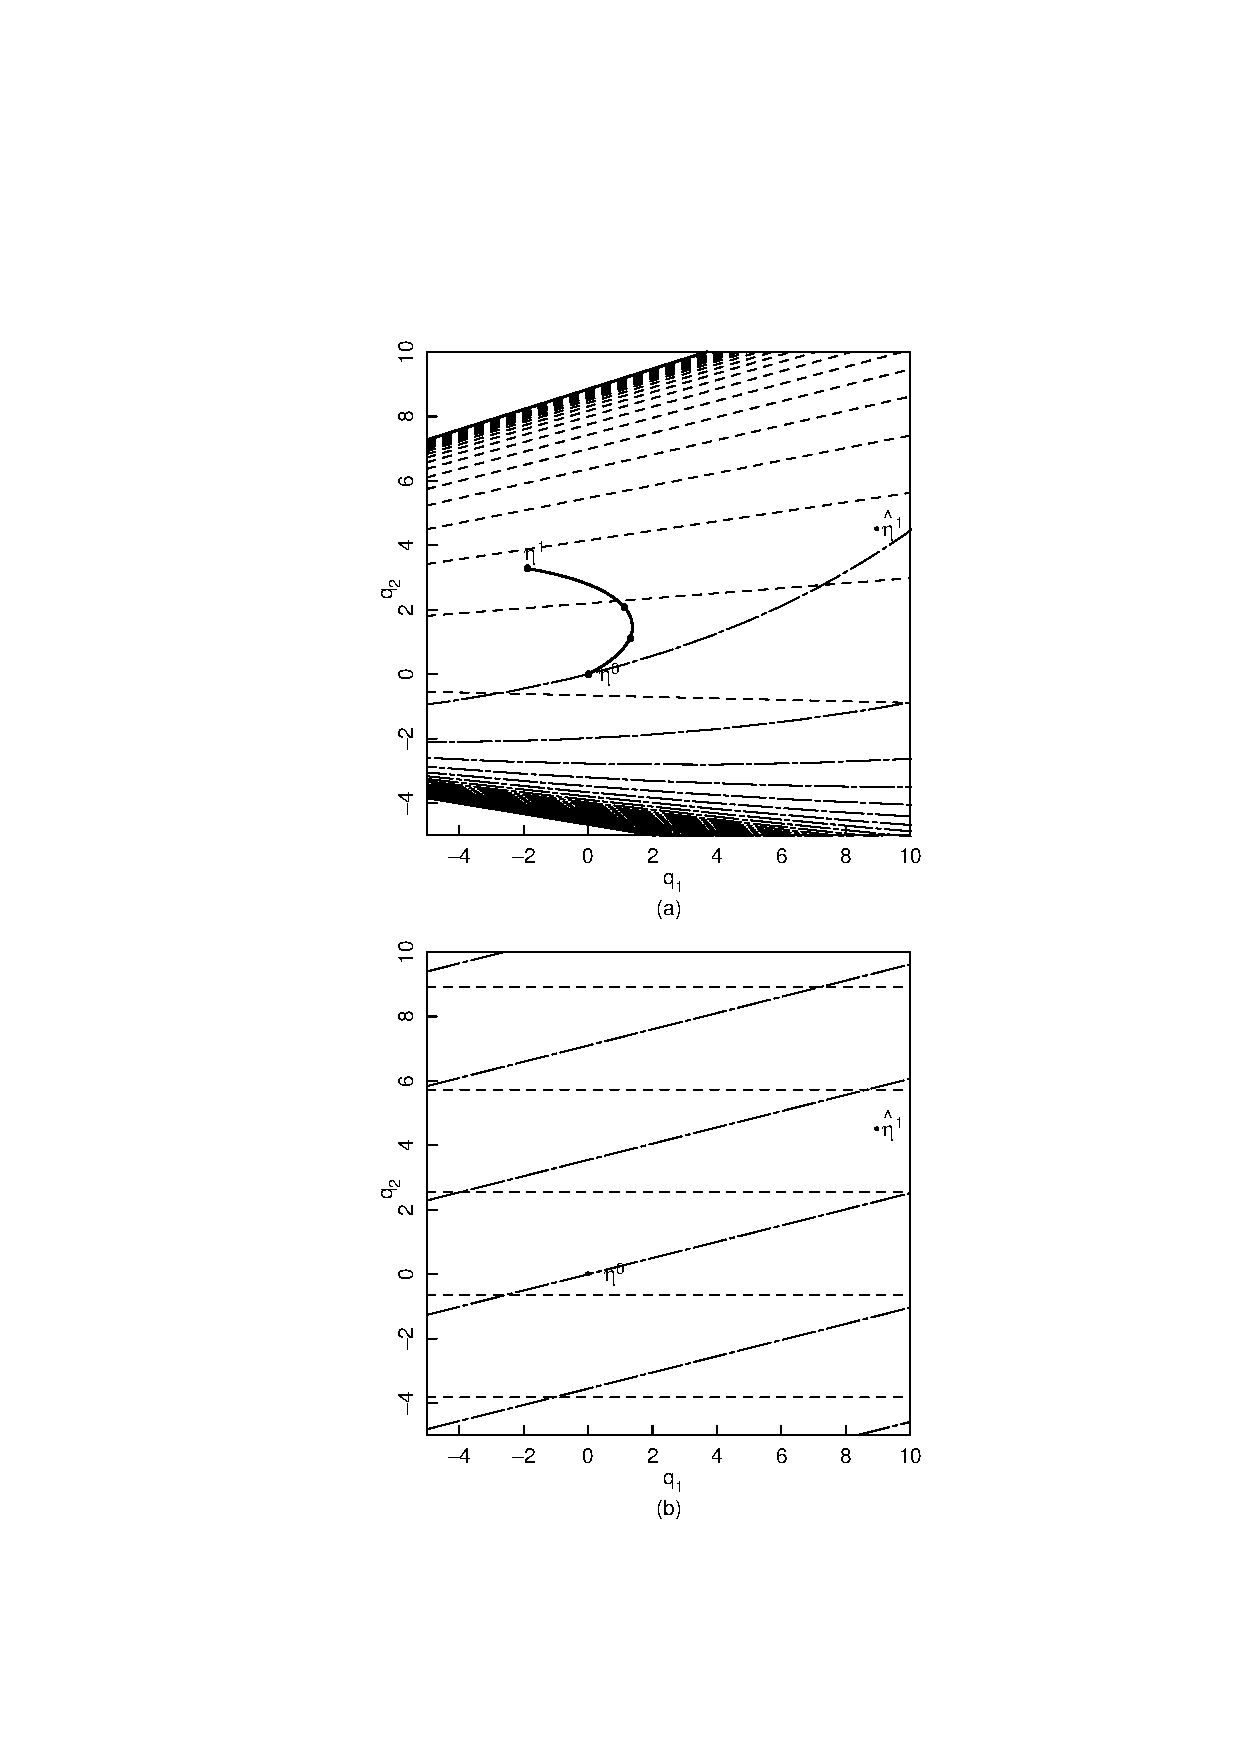
\includegraphics{2BODpeffects}}%,width=\textwidth}}
    \caption[Gauss-Newton increment]{\label{fig:BODpeffects}
    A geometric interpretation of calculation of the Gauss--Newton
    increment using the BOD data set (continued).
    The points $\boeta^0$and $\hat{ \boeta}^1$ are shown in the
    tangent planes together with the parameter curves in part $a$ and
    the linear approximation parameter lines in part $b$.
    In part $a$ we also show the projection $\boeta^1$ of the point
    $\boeta ( \btheta^0+\bdelta^0 )$.
    The curve (heavy solid line) joining $\boeta^0$ to $\boeta^1$ is
    the projection of $\boeta ( \btheta^0+\lambda\bdelta^0 )$ for
    $0\le\lambda\le1$.
    The points corresponding to $\lambda = 0.25$ and $0.5$ are marked.
    }
  \end{figure}

In Figure \ref{fig:BODpeffects}$a$ we show the parameter curves for
$\theta_1 = 20,30,\ldots$ and
$\theta_2 = 0.2,0.4,\ldots$ projected onto the tangent plane.
In Figure \ref{fig:BODpeffects}$b$ we show the corresponding linear
approximation lines on the tangent plane.
\index{parameter!linear approximation line to curve}
In this case, the linear approximation lines
do not match the true parameter curves well at all.
Also shown on the tangent planes are the points $\boeta^0$
and $\hat{ \boeta}^1$, and in Figure \ref{fig:BODpeffects}$a$ the
projection of the curve
$\boeta ( \btheta^0 + \lambda  \bdelta^0 )$ for
$0 \le \lambda \le 1$.
The points corresponding to $\lambda = 0.25, 0.5$, and
$1$ ($\boeta^1$) are marked.

Because the uniform coordinate assumption is not valid this far from
$\btheta^0$,
\index{uniform coordinate!assumption}
the points $\hat{ \boeta}^1$ and $\boeta^1$ are widely
separated, and in fact $\boeta^1$ is farther from
$\hat{ \boeta}^1$ than is $\boeta^0$.
In this case, the reduced step, $\lambda =0.5$, is successful,
as was shown in Example BOD \ref{bod:stephalf}.
\end{example}

To summarize, geometrically we are using local information to
generate a tangent plane with a linear coordinate system dictated
by the derivative vectors, projecting the residual vector onto
that tangent plane, and then mapping the tangent plane
coordinates to the parameter plane using the linear mapping.

\subsection{Convergence}

We have indicated that the Gauss--Newton iterative method is
continued until the values of $\btheta$ on successive
iterations stabilize.
This can be measured by the size of each parameter increment
relative to the previous parameter value, which is the basis for
one of the common criteria used to declare convergence
\index{convergence!criterion}
\cite{bard:1974,drap:smit:1981,jenn:samp:1968,rals:jenn:1978,kenn:gent:1980}.
%(Bard, 1974; Draper and Smith, 1981; Jennrich and Sampson, 1968;
%Kennedy and Gentle, 1980; Ralston and Jennrich, 1978).
%\glossary{ Bard, Y.}
%\glossary{ Draper, N.R.}
%\glossary{ Smith, H.}
%\glossary{ Jennrich, R.I.}
%\glossary{ Sampson, P.F.}
%\glossary{ Kennedy, W.J.Jr.}
%\glossary{ Gentle, J.E.}
%\glossary{ Ralston, M.L.}
Another criterion for convergence used, for example, in
SAS \cite{SAS:1985:stat}, is that the relative
change in the sum of squares on successive iterations be small.
\citeasnoun{Himm:1972} recommends that both these criteria be used,
%\glossary{Himmelblau, D.M.}
since compliance with one does not imply compliance with the other.
However, compliance even with both relative change criteria does
not guarantee convergence, as discussed in \citeasnoun{bate:watt:1981:tech}.
%\glossary{ Bates, D.M.}
%\glossary{ Watts, D.G.}
\citeasnoun{kenn:gent:1980} mention a relative step size criterion
%\glossary{ Kennedy, W.J.Jr.}
%\glossary{ Gentle, J.E.}
as well as relative change in the sum of squares and gradient
size criteria.
\citeasnoun{cham:1977} quotes several other criteria, including the size
%\glossary{ Chambers, J.M.}
of the gradient, the size of the Gauss--Newton step, and the
fact that the residual vector should be orthogonal to the
derivative vectors; but no scale is suggested.

The main criticism of these criteria is that they indicate lack of
progress rather than convergence.
In most cases, of course, lack of progress occurs because a
minimum is encountered: nevertheless, situations can occur where
the parameter increment and sum of squares convergence criteria
indicate lack of progress and yet a minimum has not been reached.

Examination of the geometry of nonlinear least squares provides a
better procedure for determining convergence
(Bates and Watts, 1981b).
%\cite{Bates Watts 1981 techno}
%\glossary{ Bates, D.M.}
%\glossary{ Watts, D.G.}
\index{convergence!geometry}
\index{geometry!of convergence}
We know that a critical point is reached whenever the residual
vector $\by - \boeta ( \btheta )$ is orthogonal to
the expectation surface and therefore to the tangent plane to
the expectation surface at $\boeta ( \btheta )$.
We can thus adopt orthogonality of the residual vector to the
tangent plane as a convergence criterion.
\index{convergence!orthogonality criterion}

In practice, it would be unusual to obtain exact orthogonality in
the presence of numerical roundoff, and we do not want to waste
effort calculating small changes in the parameter vector while
trying to achieve perfect orthogonality.
We therefore need to establish a \emph{tolerance level}
\index{convergence!tolerance level}
which we
can use to declare the residual vector to be ``sufficiently orthogonal.''
One way to do this is to consider the statistical variability in
the least squares estimates.

If we assume that the tangent plane forms a good approximation to
the expectation surface near $\hat{ \btheta}$, so a likelihood
region for $\btheta$ roughly corresponds to a disk on the
tangent plane with a radius proportional to
$\sqrt{S ( \hat{ \btheta} )}$, then we can measure the relative
offset of the current parameter values from the exact least
squares estimates by calculating the ratio of the length of the
component of the residual vector in the tangent plane to
$ \sqrt {S ( \hat{ \btheta} )}$.
When this ratio is small, the numerical uncertainty of the least
squares estimates is negligible compared to the statistical
uncertainty of the parameters.

Unfortunately, this criterion involves the unknown least squares
vector $\hat{ \btheta}$.
We therefore modify the criterion by substituting the current estimate,
$\btheta^i$, for $\hat{ \btheta}$, and
measure the scaled length of the tangent plane component of the residual
vector relative to the scaled length of the orthogonal component of the
residual vector at $\btheta^i$.
This leads to a \emph{relative offset convergence criterion}
\index{convergence!relative offset criterion}
  \begin{equation}\label{eqn:2.7}
  \frac{{\norm \bQ_1 \trans ( \by - \boeta ( \btheta^i ) ) \norm} / \sqrt P
  }{{\norm \bQ_2 \trans ( \by - \boeta ( \btheta^i ) ) \norm} /
  \sqrt{N -P}}
  \end{equation}
where $\bQ_1$ and $\bQ_2$ are the first $P$ and last $N - P$
columns respectively of the matrix $\bQ$ from a \emph{QR} decomposition
of $\bV$.
The criterion is related to the cotangent of the angle
that the residual vector makes with the tangent plane, so that a
small relative offset corresponds to an angle near 90$^\circ$.

To declare convergence, we require the relative offset to be less than
0.001, reasoning that any inferences will not be
affected materially by the fact that the current parameter vector is less
than 0.1\% of the radius of the confidence
region disk from the least squares point.
\label{rum:4}
\begin{example}

We illustrate the convergence criterion and its development with the
2-observation Rumford example.
We wish to test whether the parameter value
$\theta=0.01$ could be considered a point of convergence.
  \begin{figure}
    \centerline{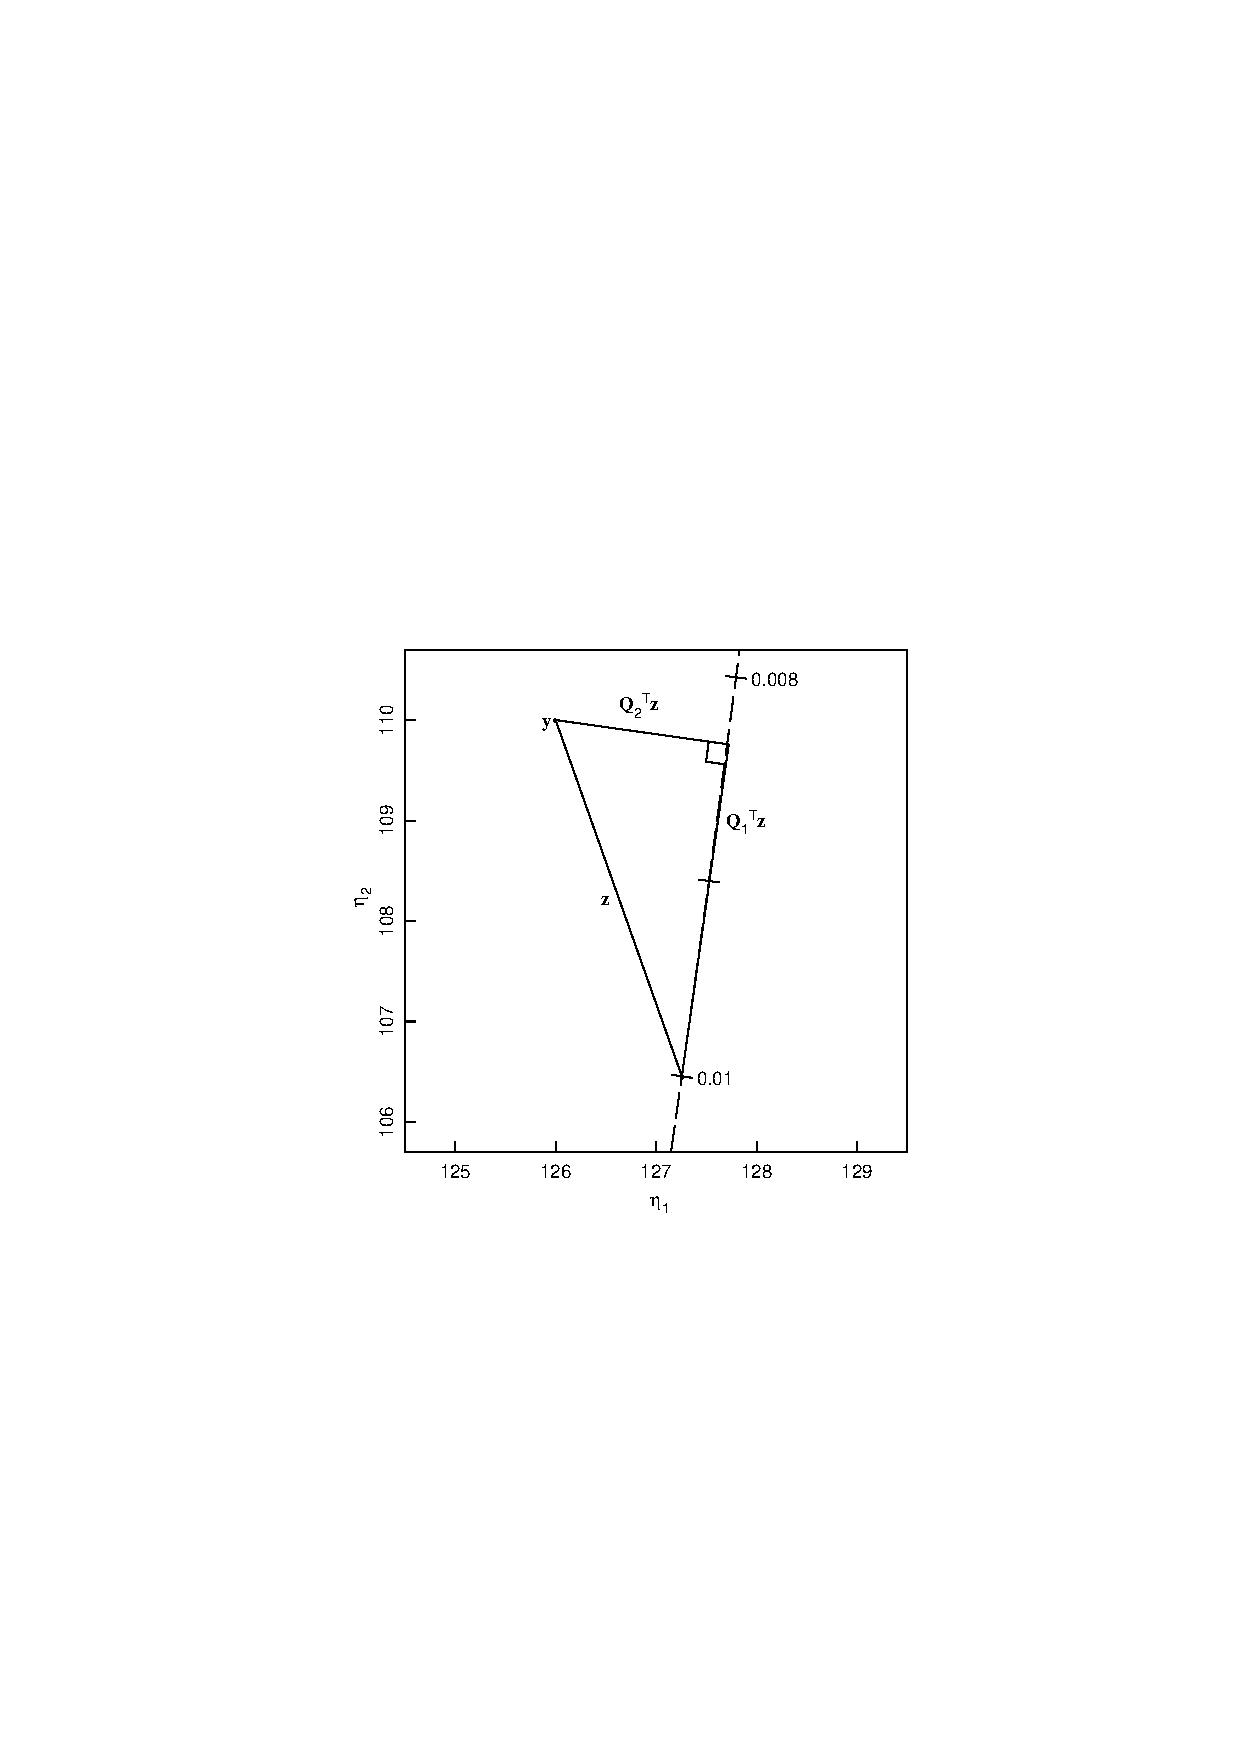
\includegraphics{2RUM2convge}}%,width=\textwidth}}
    \caption[Relative offset for the Rumford 2-case example]{
    \label{fig:RUM2convge}
    A geometric interpretation of relative offset using the 2-case
    Rumford data.
    A portion of the expectation surface (dashed line) is shown in
    the expectation space together with the residual vector $\bz$ and
    its projections into the tangent plane ($\bQ_1 \trans \bz$)
    and orthogonal to the tangent plane ($\bQ_2 \trans \bz$).
    }
  \end{figure}
Figure \ref{fig:RUM2convge} shows a portion of the expectation surface, the
observation point $\by$, and the tangent plane at
$\boeta ( 0.01 )$.
Also shown is the component of the residual vector in the tangent
plane, $\bQ_1 \trans \bz$, and the component orthogonal to
the tangent plane, $\bQ_2 \trans \bz$.
The tangent plane component is large relative to the orthogonal
component, having a relative offset of 1.92, and so we conclude
that the residual vector at $\theta = 0.01$ is not sufficiently
orthogonal for us to accept $\theta = 0.01$ as the converged
value.
\end{example}

Convergence implies that the best estimates of the
parameters have been obtained, under the assumption that the model is
adequate.
Before characterizing the precision of the
estimates using inference intervals or regions,
therefore, we should check the residuals for signs of model
inadequacy.
A complete discussion of the practical aspects of nonlinear
regression is given in Chapter 3, but in the interests of completeness
in analyzing the Puromycin and BOD data, we simply plot the residuals
versus the fitted values and using probability plots
before continuing.
\label{mic:resplots}
\begin{example}

Convergence for the Puromycin data was declared at
$\hat{ \btheta} = ( 212.7 ,  0.0641 ) \trans$, with $s^2= 119.5$
on 10 degrees of freedom.
Studentized residuals from the least squares fit are plotted in
Figure \ref{fig:PURresplots} versus
fitted values in part $a$ and as a normal probability plot in part $b$.
  \begin{figure}
    \centerline{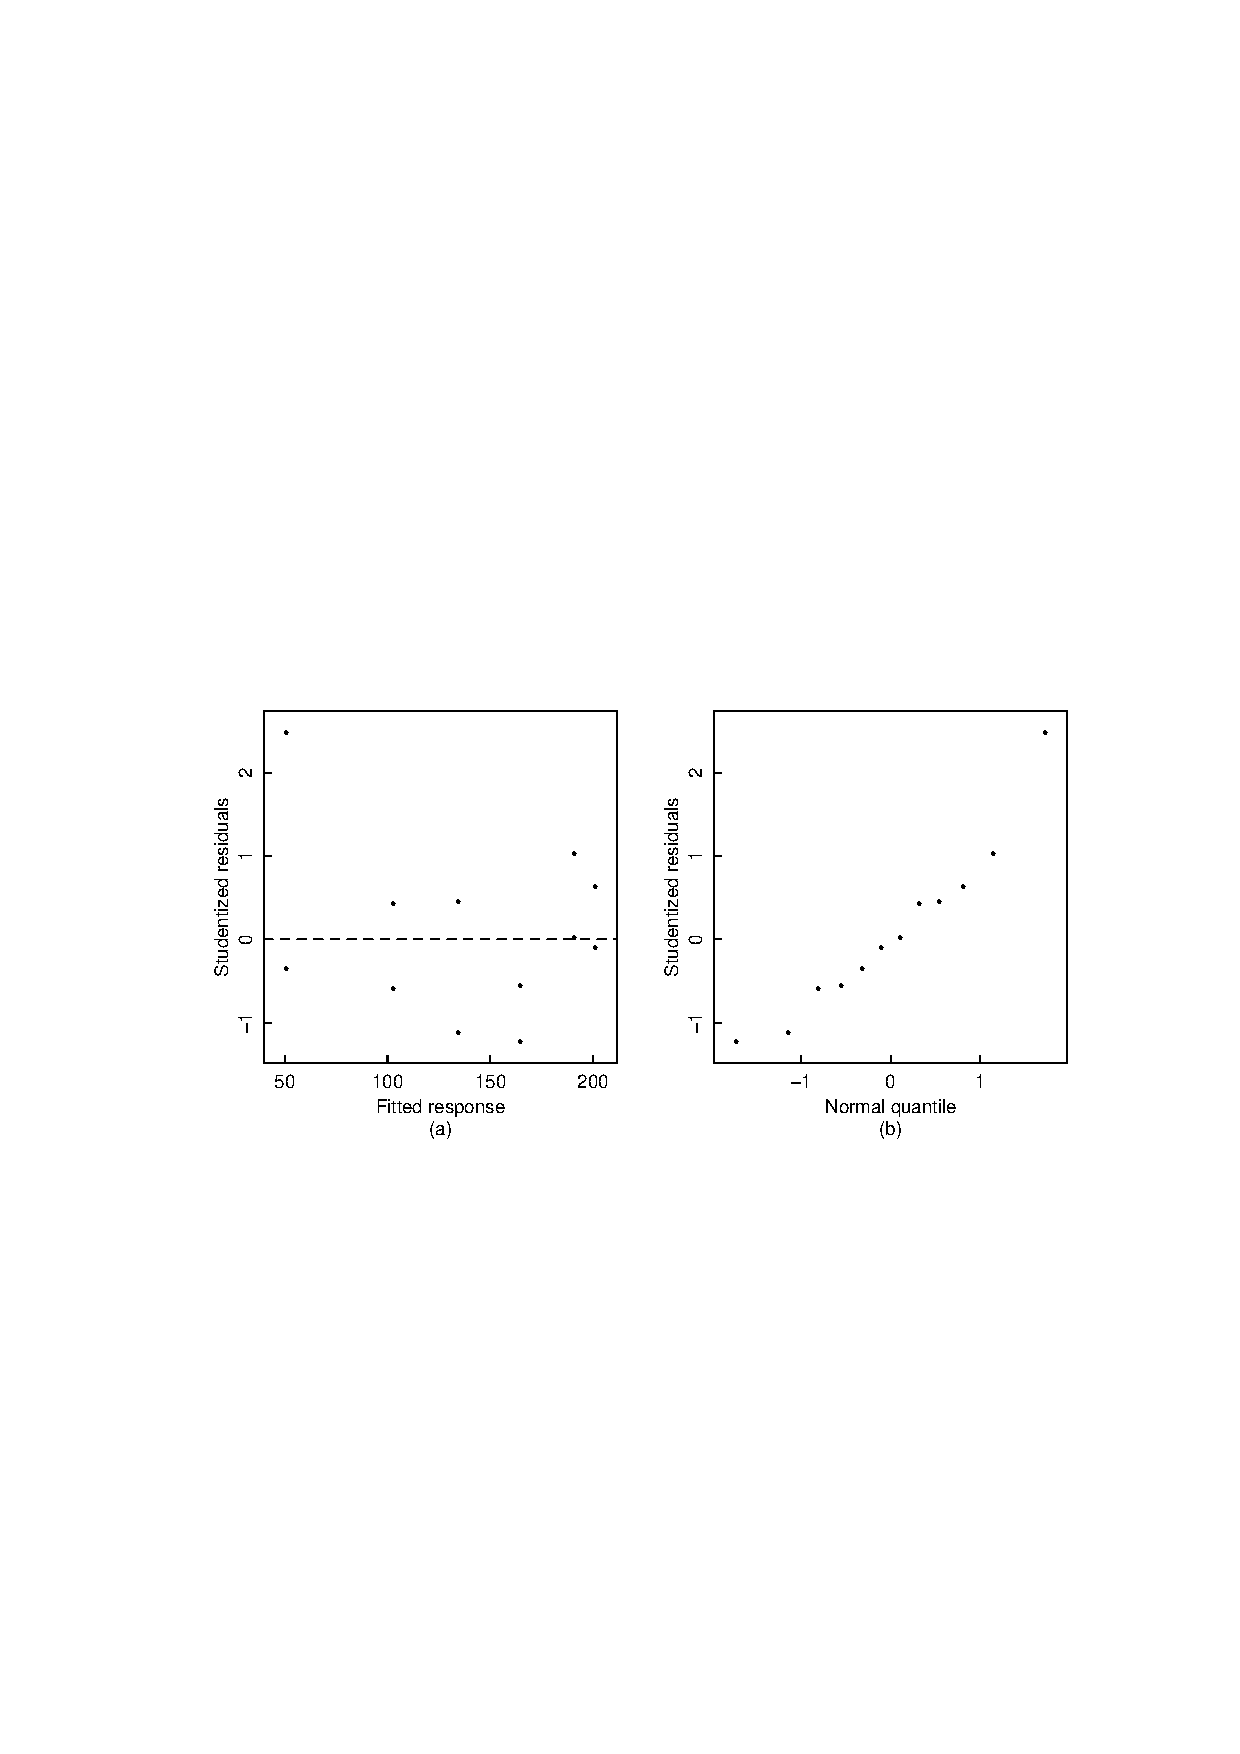
\includegraphics{2PURresplots}}%,width=\textwidth}}
    \caption[Studentized residuals for Puromycin data]{
    \label{fig:PURresplots}
    Studentized residuals for the Puromycin data plotted versus fitted values
    in part $a$ and versus normal quantiles in part $b$.
    }
  \end{figure}
Although there is one relatively large residual, the overall
fit appears adequate, and so we proceed to develop parameter
inference regions.
\end{example}
\begin{example}
\label{bod:resplots}

Convergence for the BOD data was declared at
$\hat{ \btheta} =( 19.143,  0.5311 ) \trans$, with $s^2=6.498$
on 4 degrees of freedom.
Studentized residuals from the least squares fit are plotted in
Figure \ref{fig:BODresplots} versus fitted values in part $a$ and as a
normal probability plot in part $b$.
  \begin{figure}
    \centerline{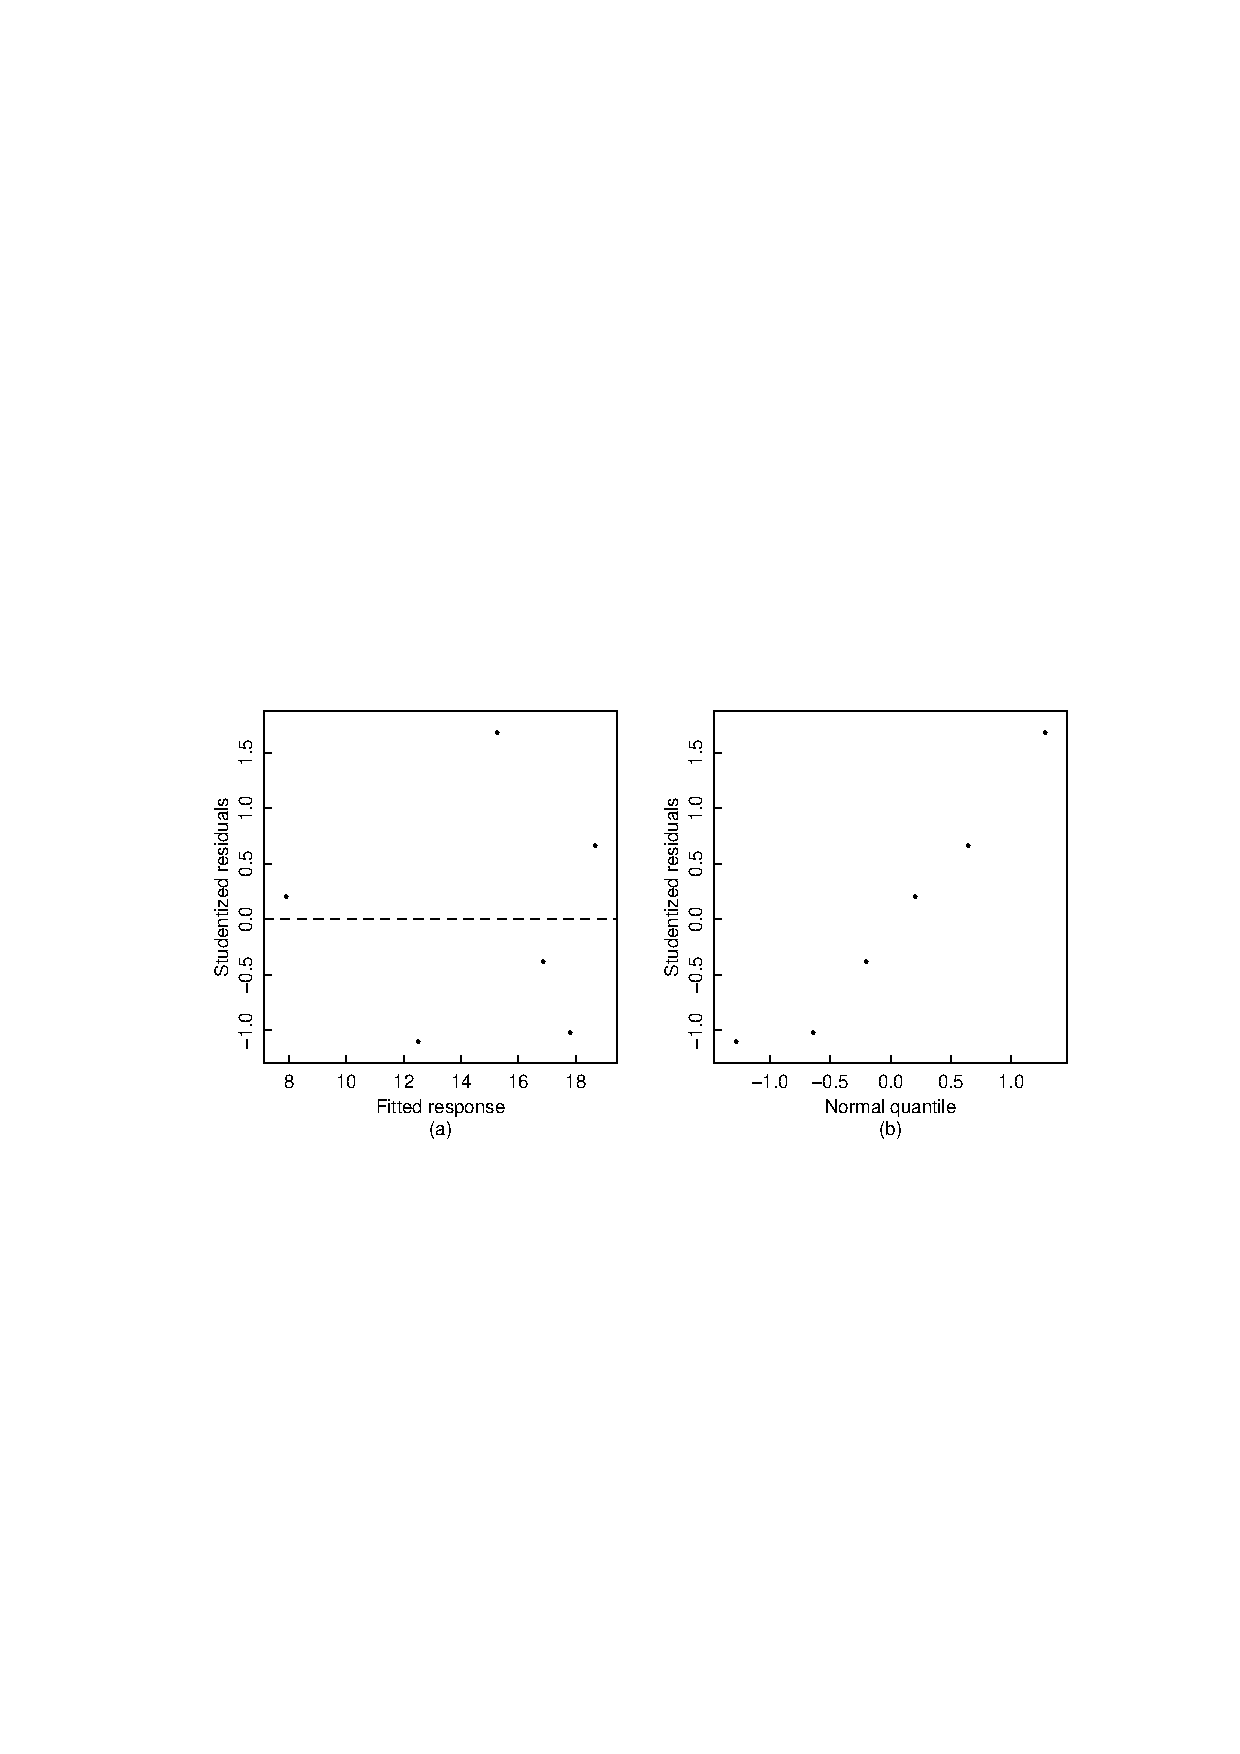
\includegraphics{2BODresplots}}%,width=\textwidth}}
    \caption[Studentized residuals for BOD data]{
    \label{fig:BODresplots}
    Studentized residuals for the BOD data plotted versus fitted values
    in part $a$ and versus normal quantiles in part $b$.
    }
  \end{figure}
Since the residuals are well behaved, we proceed to develop
parameter inference regions.
\end{example}

\section{Nonlinear Regression Inference Using the Linear Approximation}
\sectionmark{Inference Using Linear Approximation}

In the Gauss--Newton algorithm for calculating $\hat{ \btheta}$,
the derivative matrix $\bV$ is evaluated at each iteration and used
to calculate the increment and the convergence criterion.
It is natural, then, to apply the linear approximation to
\emph{inference} for nonlinear models with the derivative matrix
\index{inference!in nonlinear regression}
\index{inference!linear approximation}
evaluated at the least squares parameter estimates.
This yields approximate likelihood, confidence, or Bayesian
HPD regions, based on
  \begin{equation}\label{eqn:2.7a}
  \boeta ( \btheta ) = \boeta ( \hat{ \btheta} ) +
  \hat{ \bV} ( \btheta - \hat{ \btheta} )
  \end{equation}
\subsection{Approximate Inference Regions for Parameters 2 3 1}

Recall that in the linear case, a $1-\alpha$
parameter inference region can be expressed as [cf. (1.9)]
\index{parameter!inference region}
  \begin{equation}\label{eqn:infreg}
  ( \bbeta - \hat{ \bbeta} ) \trans \bX \trans \bX
  ( \bbeta - \hat{ \bbeta} )  \le  P s^2 \FPNP
  \end{equation}
Geometrically this region results because the expectation surface
is a plane and the residual vector is orthogonal to that plane,
so the region of plausible values on the expectation plane is a
disk.
Taking the disk through the linear mapping relating points on the
expectation plane to points on the parameter plane, then maps the
disk to an ellipsoid on the parameter plane.

Approximate inference regions for a nonlinear model are defined,
\index{parameter!approximate inference region}
by analogy with equation (\ref{eqn:infreg}), as
  \begin{equation}\label{eqn:linregion}
  ( \btheta - \hat{ \btheta} ) \trans \hat{ \bV} \trans \hat{ \bV}
  ( \btheta - \hat{ \btheta} ) 
  \le P s^2 \FPNP
  \end{equation}
or equivalently
  \begin{equation}\label{eqn:2.12}
  ( \btheta - \hat{ \btheta} ) \trans \hat{ \bR}_1 \trans \hat{ \bR}_1
  ( \btheta - \hat{ \btheta} ) 
  \le P s^2 \FPNP
  \end{equation}
where the derivative matrix $\hat{ \bV} = \hat{ \bQ}_1 \hat{ \bR}_1$
is evaluated at $\hat{ \btheta}$.
The boundary of this inference region (\ref{eqn:2.12}) is [cf. (1.28)]
  \begin{equation}\label{eqn:2.13a}
  \left\{\btheta = \hat{{\btheta}}+\sqrt{P s^2 \FPNP}\hat{{\bR}}_1^-1\bd
  |  \norm \bd \norm = 1 \right\}
  \end{equation}

Similarly, the approximate standard error for $\theta_p$ is $s$
times the
\index{parameter!approximate standard error}
\index{standard error!approximate}
length of the $p$th row of $\hat{ \bR}_1^-1$'-1p'
[cf. (1.33)].
Approximate correlations and standard errors for the parameters are easily
\index{parameter!approximate correlations}
calculated by factoring $\hat{ \bR}_{-1}$ into a
diagonal matrix [cf. (1.34)] giving the lengths of
the rows of $\hat{ \bR}^-1$ and a matrix with unit length rows
as described in Section 1.2.3.
The parameter approximate correlation matrix is calculated as in (1.35).
\label{mic:8}
\begin{example}

Convergence for the Puromycin data was declared at
$\hat{ \btheta} = ( 212.7 ,  0.0641 ) \trans$, with $s^2= 119.5$
on 10 degrees of freedom and
\begin{displaymath}
  \hat{ \bR}_1 =
  \begin{bmatrix}
    -2.4441 & 1568.7 \\
    0       & 1320.3 
  \end{bmatrix}
\end{displaymath}

The 95 and 99\% approximate joint inference regions were
obtained by evaluating (\ref{eqn:2.13a}) with
$\bd =( \cos\omega , \sin\omega ) \trans$ and are plotted in
Figure \ref{fig:MIClinregion}.
  \begin{figure}
    \centerline{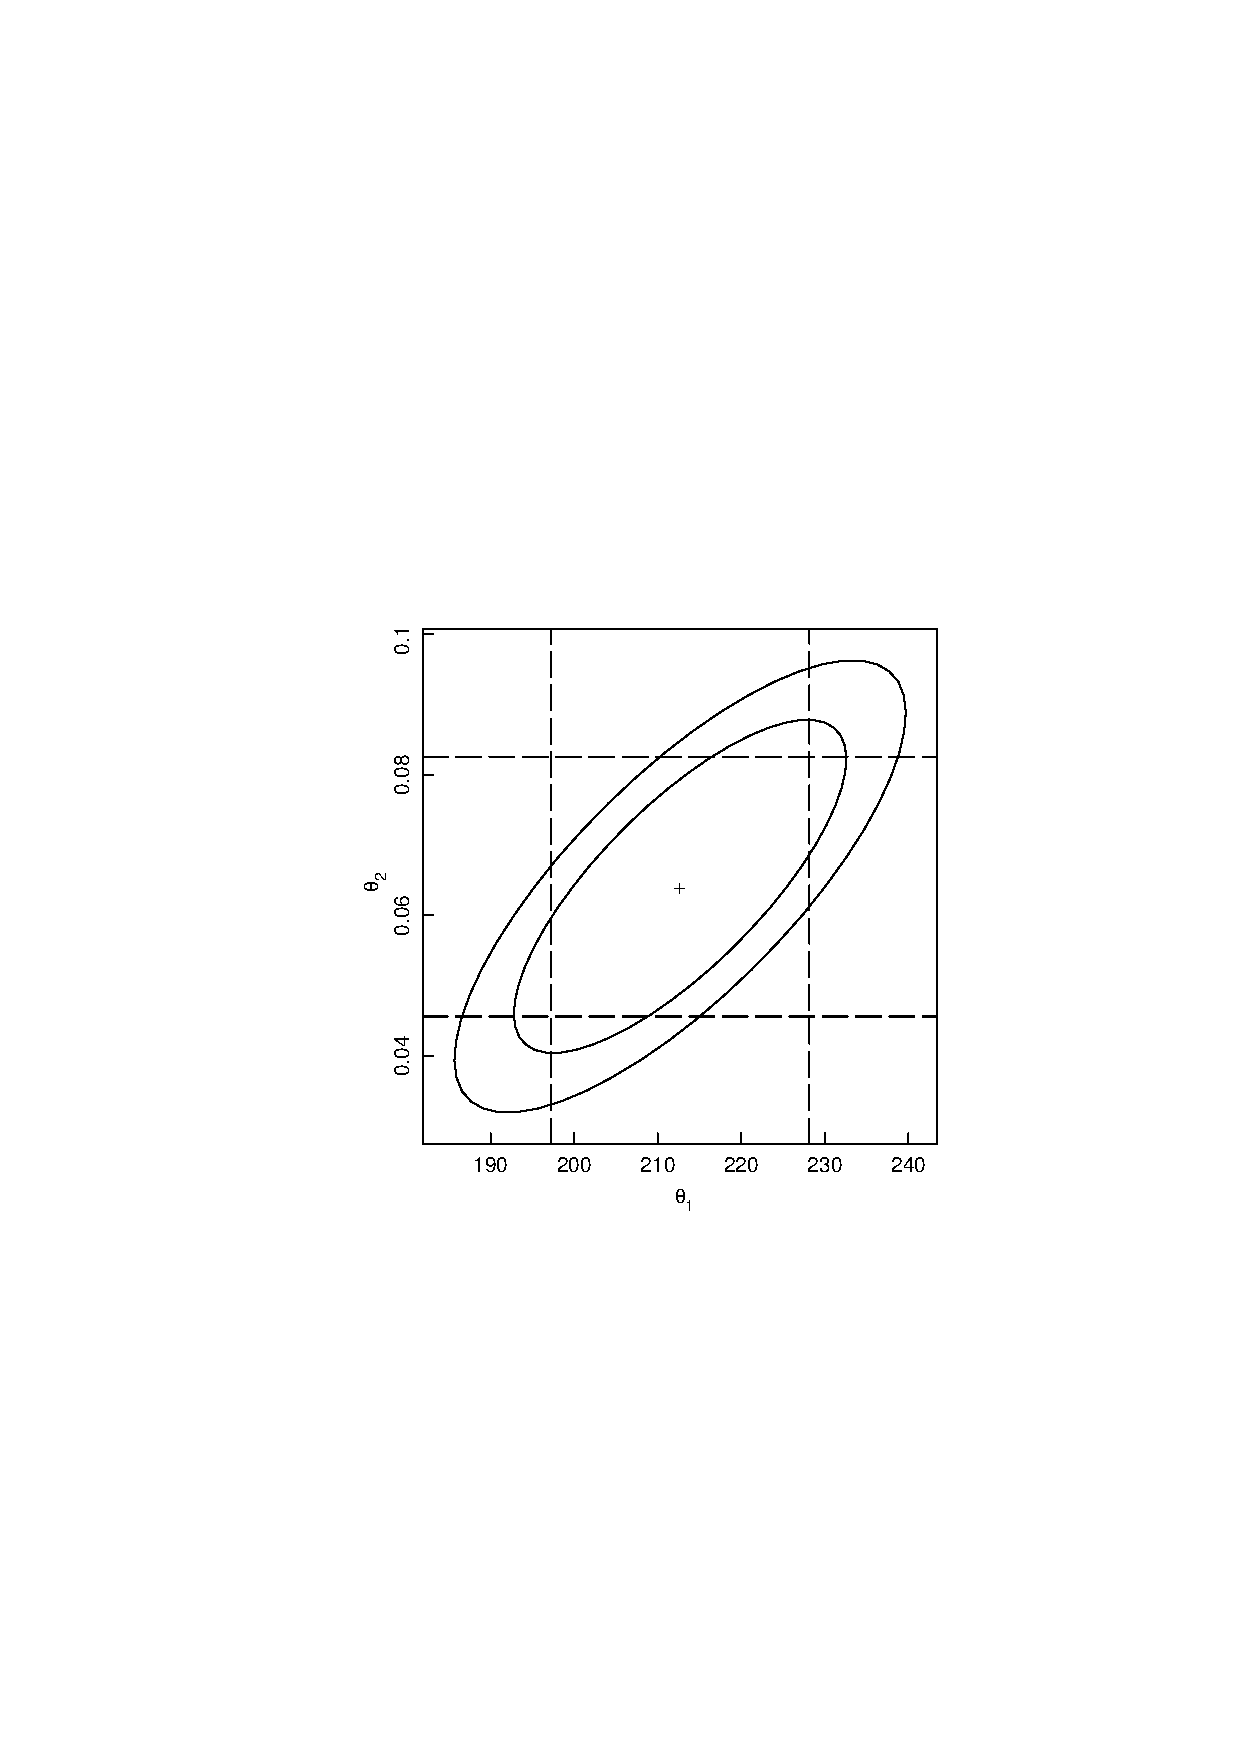
\includegraphics{2MIClinregion}}%,width=\textwidth}}
    \caption{\label{fig:MIClinregion}
    Parameter approximate inference regions for the Puromycin data.
    We show the least squares estimates ($+$),
    the parameter joint 95 and 99\% inference regions (solid lines),
    and the marginal 95\% inference intervals (dashed lines).
    }
  \end{figure}
To calculate approximate marginal inference intervals, we factor
\begin{eqnarray*}
  \hat{ \bR}_1^{-1}&=&
  \begin{bmatrix}
    -0.4092 & 0.4861\\
    0      & 0.0007574
  \end{bmatrix}\\
  &=&\begin{bmatrix}0.6354&0\\0&0.0007574\end{bmatrix}
  \begin{bmatrix}
    -0.6439 & 0.7651\\
    0       & 1.0000
  \end{bmatrix}
\end{eqnarray*}
so the approximate standard errors are 6.95 and
$8.28 \times10^-3$ and the approximate correlation between
$\theta_1$ and $\theta_2$ is 0.77.
A 95\% approximate marginal inference interval for $\theta_2$, for
example, is
  \begin{displaymath}
    0.0641  \pm { \sqrt 119.5 }  (0.0007574)  t ( 10 ;  0.025 )
  \end{displaymath}
or $0.0641 \pm 0.0185$.
The 95\% marginal inference intervals for both parameters are shown as
dashed lines in Figure
\ref{fig:MIClinregion}.
\end{example}

\begin{example}\label{bod:2}
Convergence for the BOD data was declared at
$\hat{ \btheta} =( 19.143,  0.5311 ) \trans$, with $s^2 = 6.498$
on 4 degrees of freedom and
\begin{displaymath}
  \hat{ \bR}_1 =
  \begin{bmatrix}
    -1.9556 & -20.4986\\
    0 & -12.5523
  \end{bmatrix}
\end{displaymath}
giving approximate standard errors of 2.50 and 0.203.

The 95 and 99\% approximate joint inference regions are plotted in
Figure \ref{fig:BODlinregion} together with the 95\% approximate
marginal intervals.
Note that the regions include negative values for $\theta_2$, and such
values are not physically meaningful.
  \begin{figure}
    \centerline{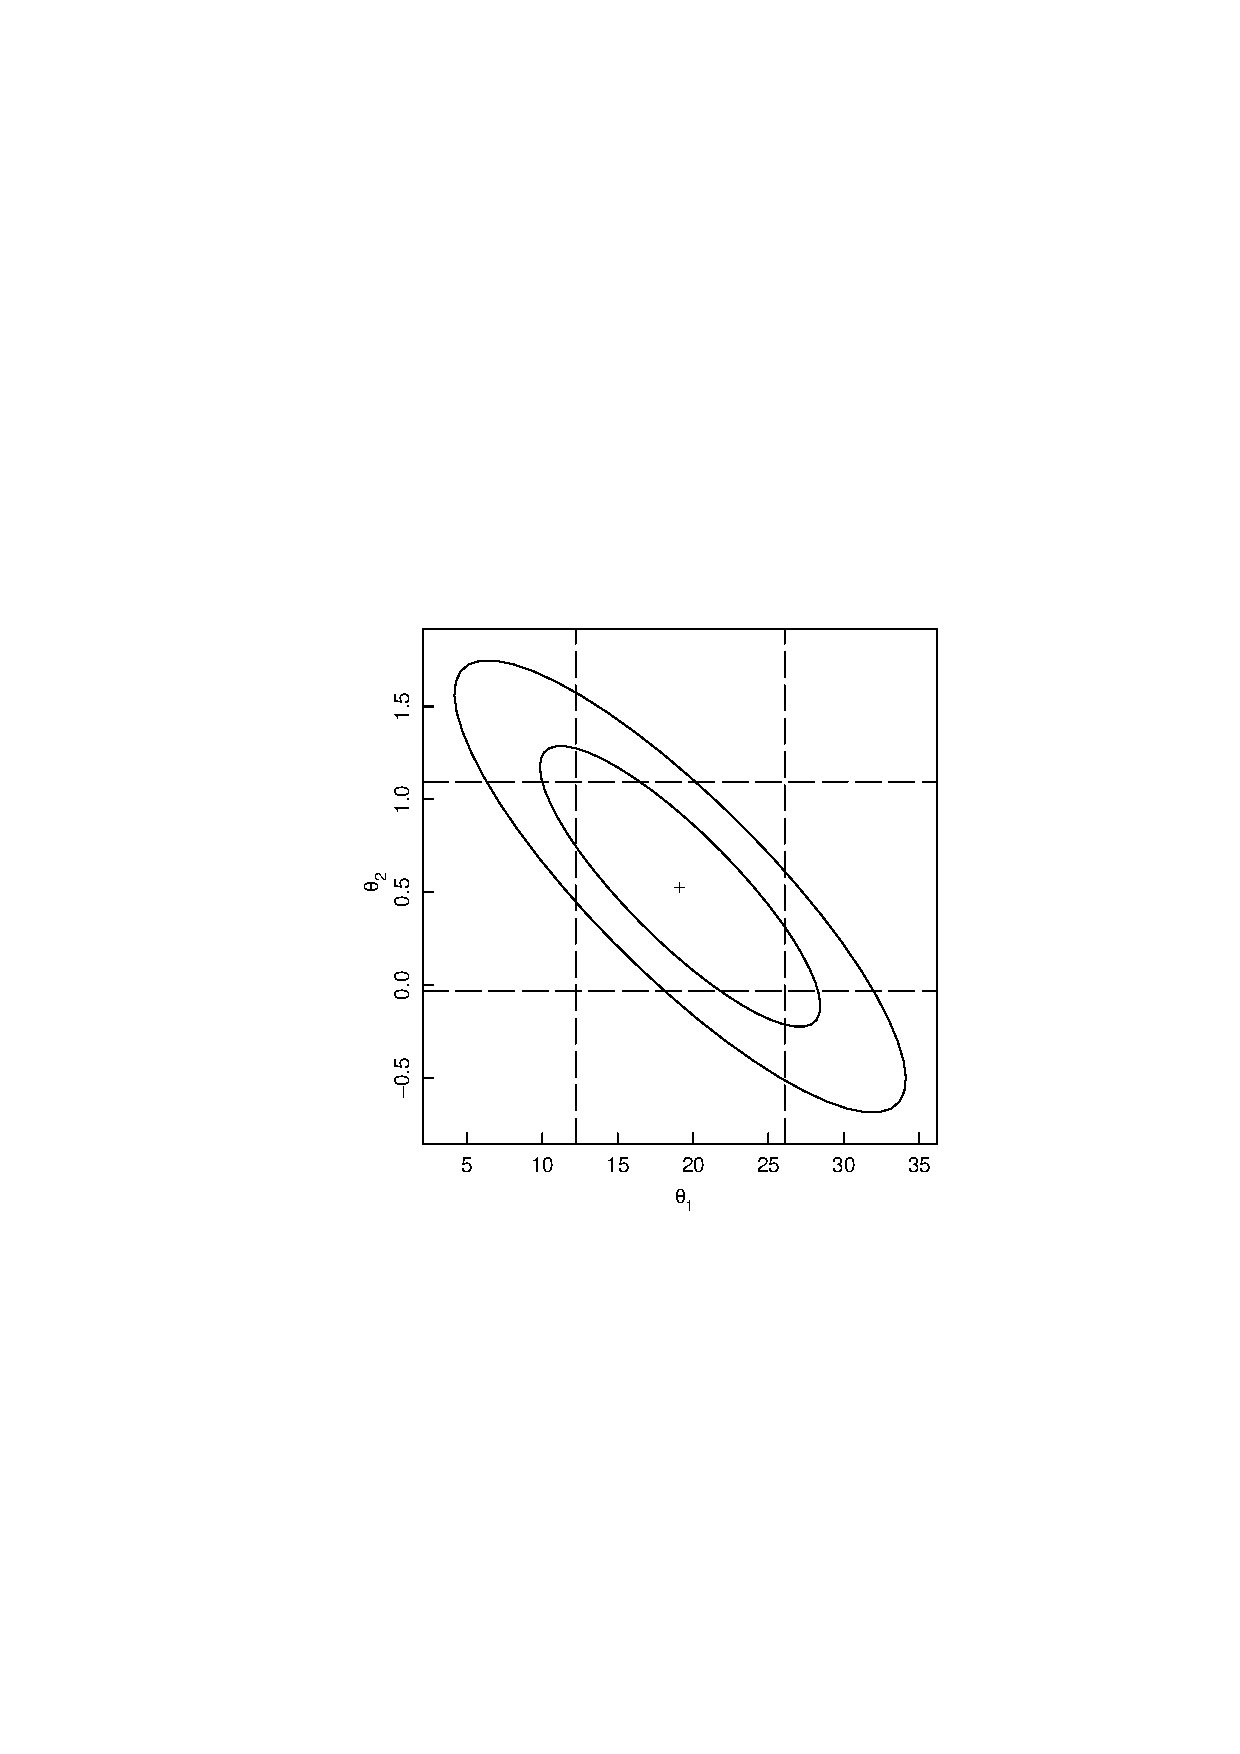
\includegraphics{2BODlinregion}}%,width=\textwidth}}
    \caption{\label{fig:BODlinregion}
    Parameter approximate inference regions for the BOD data.
    We show the least squares estimates ($+$),
    the parameter joint 95 and 99\% inference regions (solid lines),
    and the marginal 95\% inference intervals (dashed lines).
    }
  \end{figure}
The approximate correlation between $\theta_1$ and
$\theta_2$ is $-0.85$.
\end{example}

When there are more than two parameters, it is not possible to plot
the joint approximate inference region, and so it is common to
summarize the inferential situation by quoting the approximate
marginal inference intervals and the parameter correlation matrix and
by making
\index{parameter!correlation matrix}
\index{matrix!parameter correlation}
pairwise plots of the inference region.
More exact methods for summarizing the inferential situtation are
presented in Chapter 6.
\label{iso:1}
\begin{example}

Data on the reaction rate of the catalytic isomerization of
$n$-pentane to isopentane versus the partial pressures of hydrogen,
$n$-pentane, and isopentane as given in
\citeasnoun{carr:1960}%\glossary{ Carr, N.L.} are presented in
Appendix A, Section~\ref{atbl:iso}, and plotted in Figure \ref{fig:ISOdata}.
  \begin{figure}
    \centerline{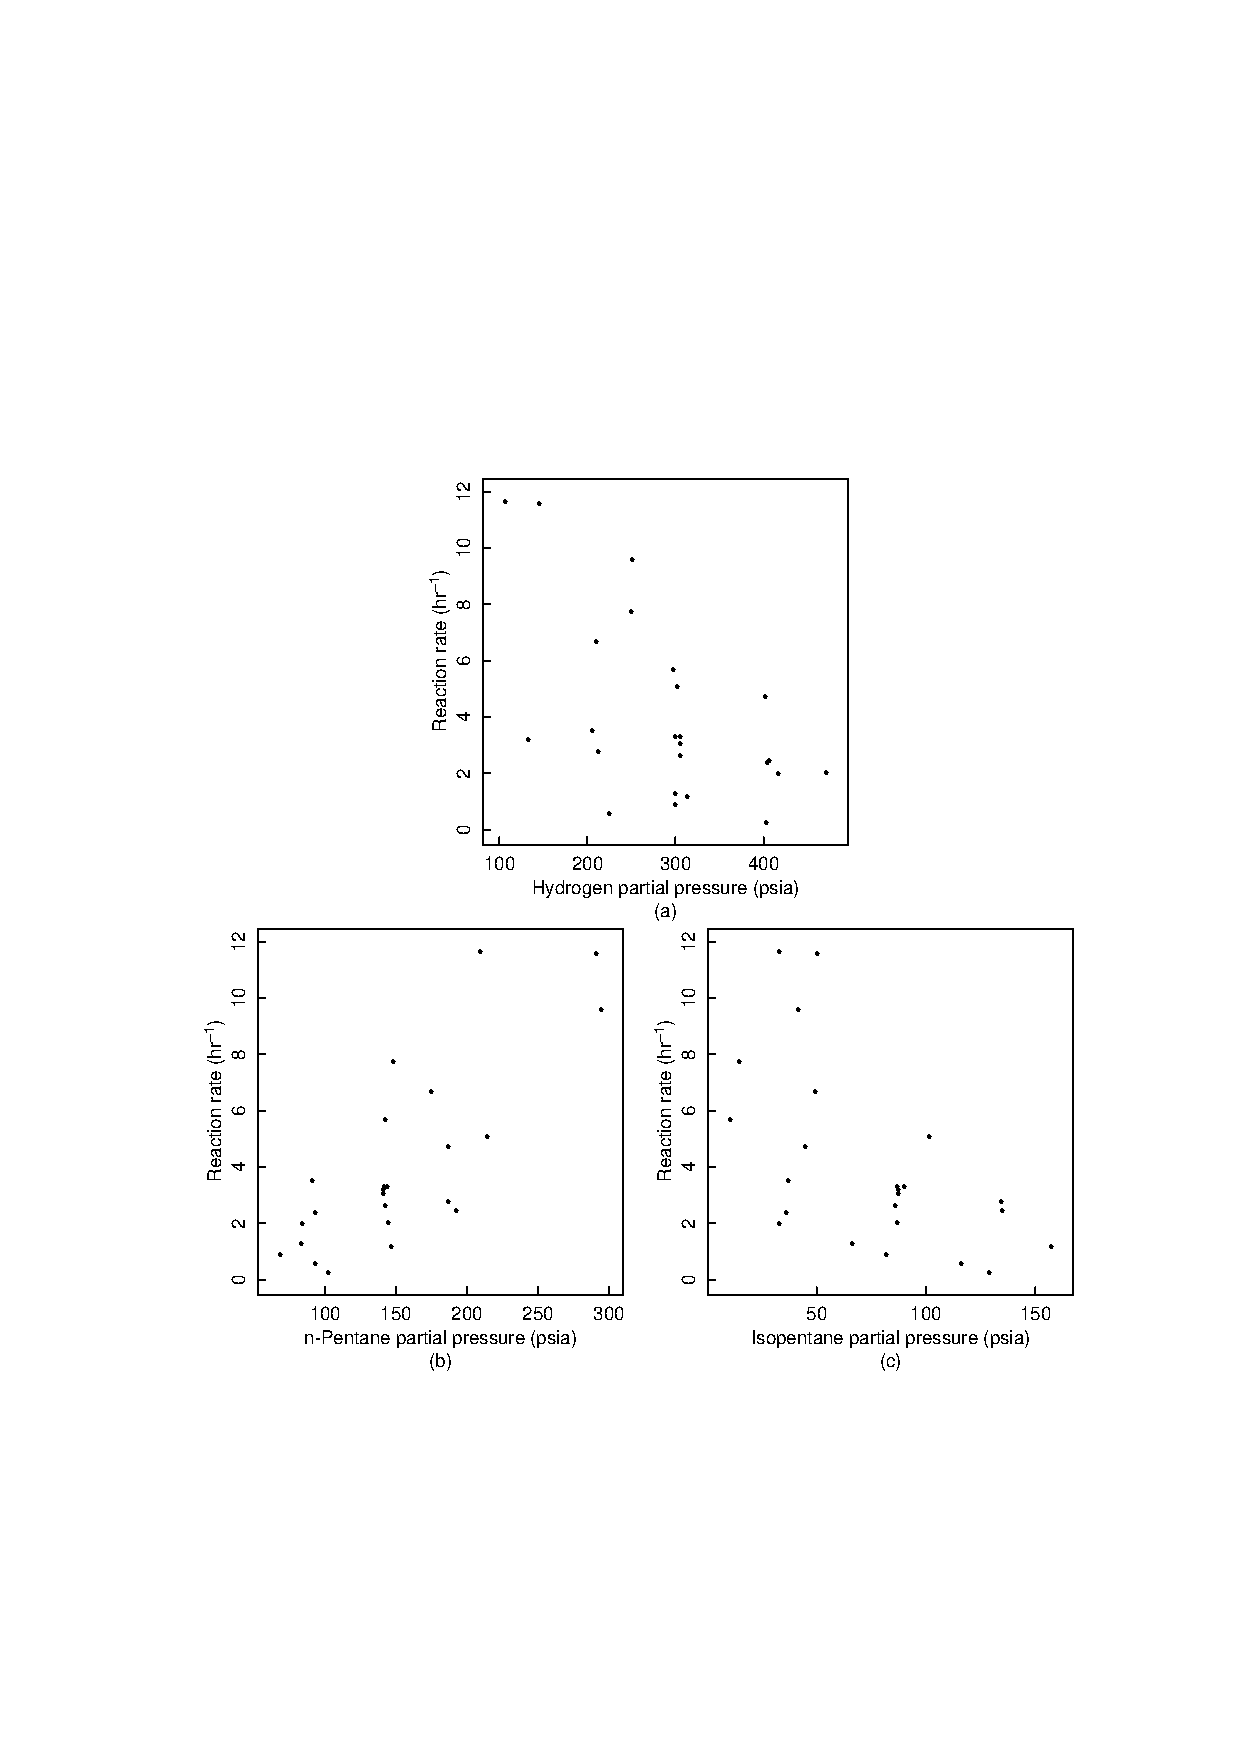
\includegraphics{2ISOdata}}%,width=\textwidth}}
    \caption{\label{fig:ISOdata}
    Plots of reaction rate of the isomerization of
    $n$-pentane to isopentane versus the partial pressures of
    hydrogen in part $a$, $n$-pentane in part $b$, and isopentane in part
    $c$.
    }
  \end{figure}
A proposed model function for these data is
  \begin{equation}\label{eqn:2.9a}
  f ( \bx , \btheta ) =
  \frac{\theta_1 \theta_3 ( x_2 - x_3 / 1.632 )}{1 + \theta_2 x_1 +
  \theta_3 x_2 + \theta_4 x_3} 
  \end{equation}
Parameter estimates and summary statistics are given in
Table \ref{tbl:isoest}, and residual plots versus the partial pressures and
  \begin{table}
%c c c c s s s
%l c c c s s s
%c c c c s s s
%c n n n 1 n 1 n 1 n.
%\_
%:::Approximate
%Parameter:Estimate:Standard:Correlation
%::Error:Matrix
%\par\vspace{2.0pt}
%\_
%$\theta_1$:35.92:8.21:1.000
%$\theta_2$:0.0708:0.1783:--\/0.805:1.000
%$\theta_3$:0.0377:0.0998:--\/0.840:0.998:1.000
%$\theta_4$:0.167:0.415:--\/0.790:0.998:0.995:1.000
%\par\vspace{4.0pt}
%\_
    \vspace{1in}
    \caption{\label{tbl:isoest}
    Parameter summary for the isomerization data}
  \end{table}
the fitted values in Figure \ref{fig:ISOresplots}.
The plots show the residuals are generally well behaved.
The summary statistics suggest potential difficulties, since
some of the correlations are extremely high and some of the standard
errors produce approximate 95\% intervals which include negative
values, but the parameters must be positive to be physically meaningful.
  \begin{figure}
    \centerline{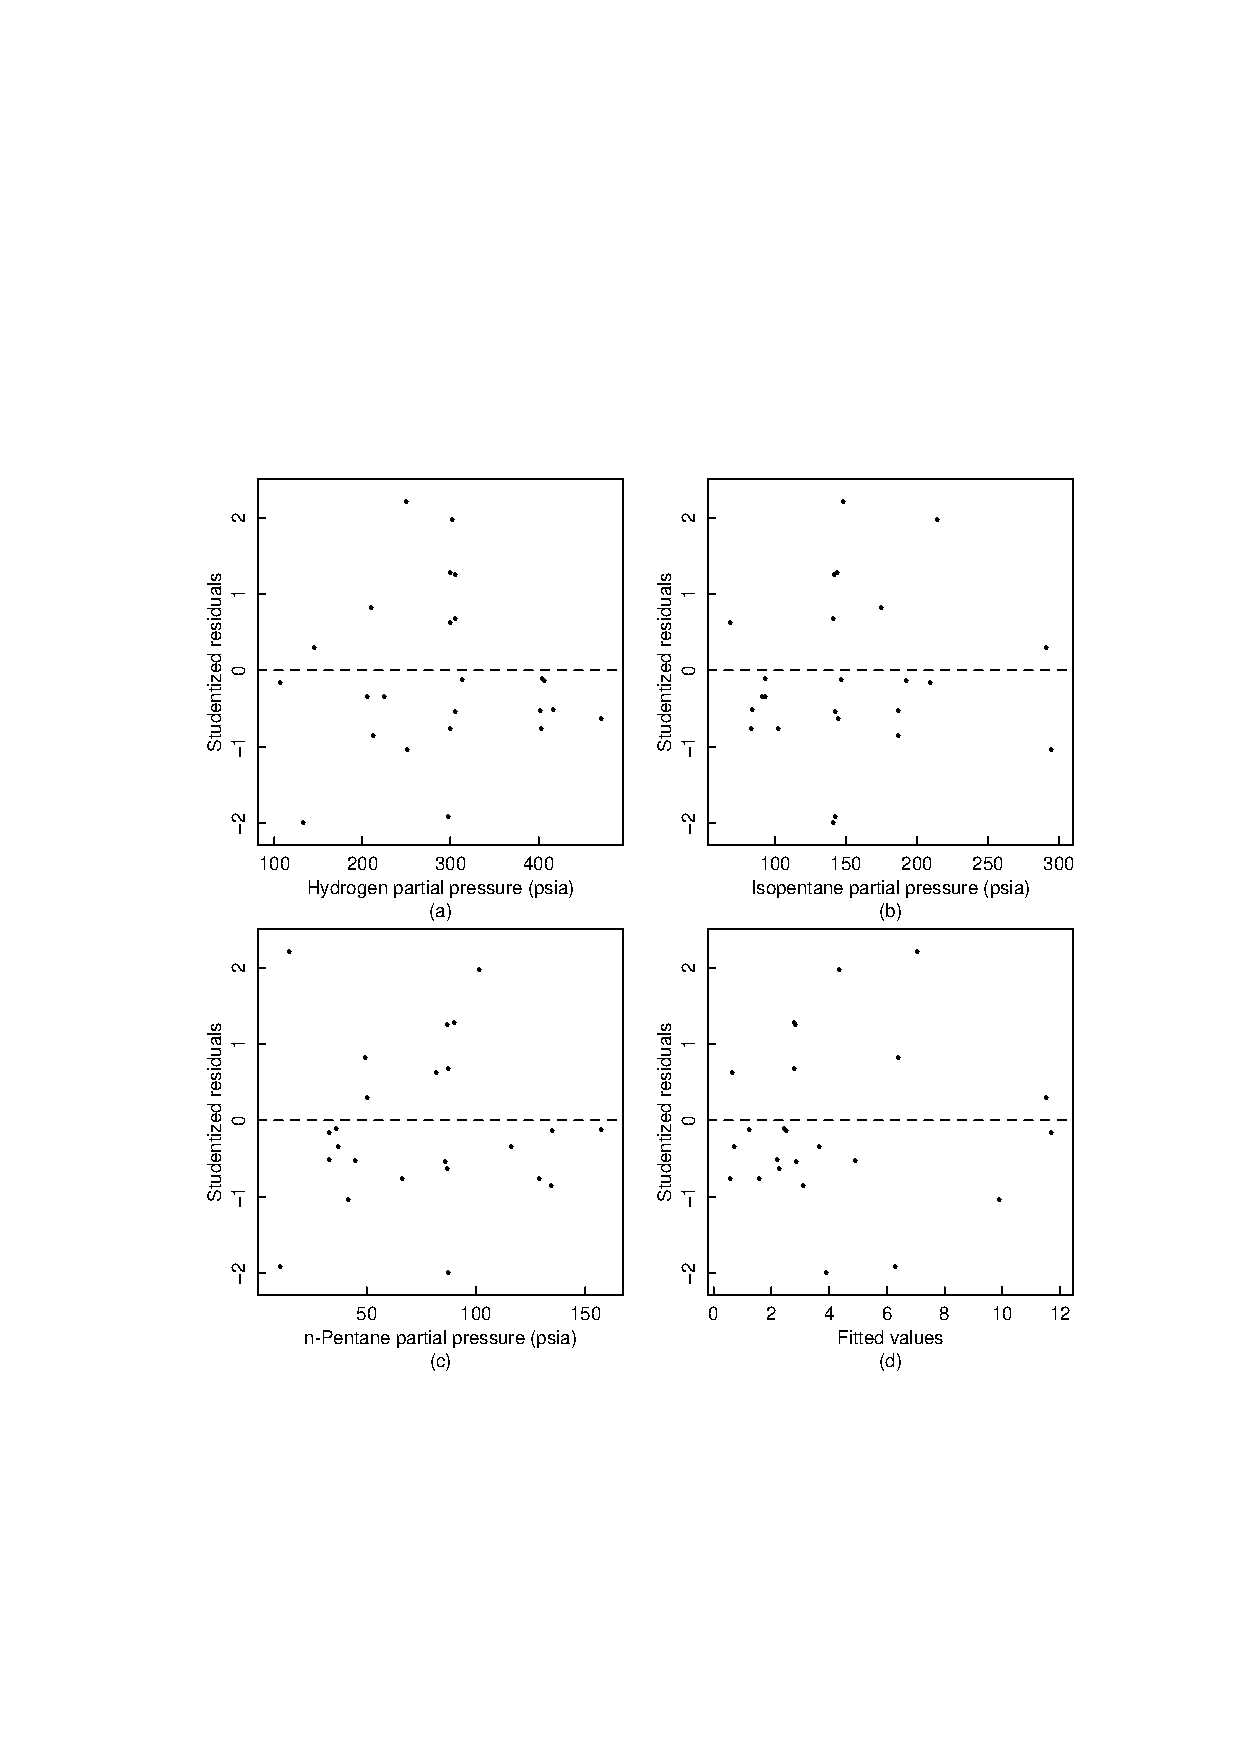
\includegraphics{2ISOresplots}}%,width=\textwidth}}
    \caption{\label{fig:ISOresplots}
    Studentized residuals for the isomerization data are plotted
    versus the partial pressures of hydrogen in part $a$, isopentane in
    part $b$, and $n$-pentane in part $c$, and versus the
    fitted values in part $d$.
    }
  \end{figure}
The pairwise plots of the parameter approximate 95\% inference
region, given in Figure \ref{fig:ISOlinregion},
  \begin{figure}
    \centerline{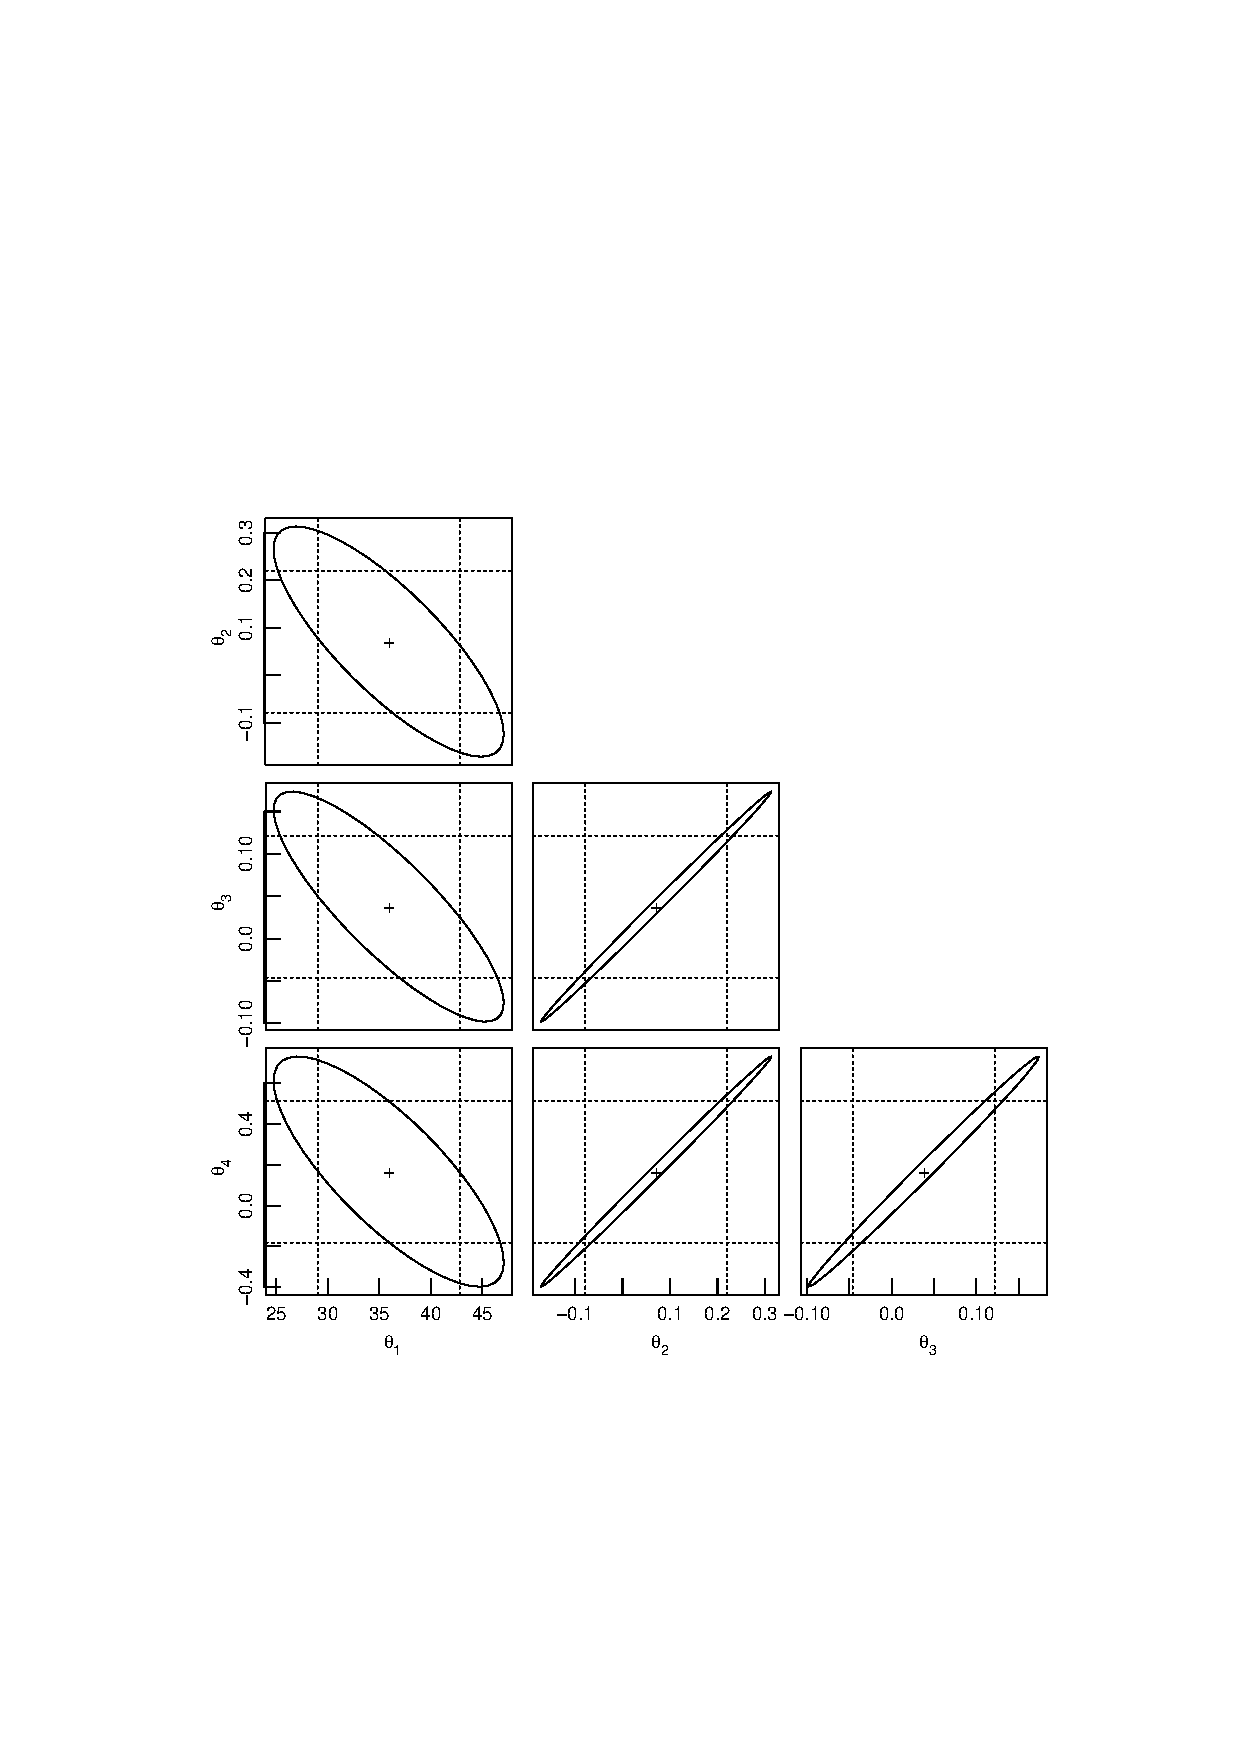
\includegraphics{2ISOlinregion}}%,width=\textwidth}}
    \caption{\label{fig:ISOlinregion}
    Pairwise plots of the parameter approximate 95\% inference region for
    the isomerization data.
    For each pair of parameters we show the least squares estimates ($+$),
    the parameter approximate joint 95\% inference region (solid line),
    and the approximate marginal 95\% inference intervals (dotted lines).
    }
  \end{figure}
clearly extend into negative parameter regions.
\end{example}

\subsection{Approximate Inference Bands for the Expected Response}

Linear approximation inference intervals and bands
\index{linear approximation!inference interval}
\index{inference!interval, linear approximation}
\index{linear approximation!inference band}
\index{inference!band, linear approximation}
for the expected response
in nonlinear regression can be generated using the analogs of the
equation for linear regression, (1.11) and (1.12).
In those equations, we simply
replace the estimated value $\bx_0 \trans \hat{ \bbeta}$ by
$f ( \bx_0 , \hat{ \btheta} )$, the matrix $\bX$ by $\hat{ \bV}$,
and the derivative vector $\bx_0$ by
\index{derivative!vector}
  \begin{displaymath}
    \bv_0=\left.\frac{\partial f ( \bx_0 , \btheta )}{\partial
    \btheta \trans }\right|_{\hat{ {\theta}}}
  \end{displaymath}
The $1 - \alpha $ approximate inference interval is then
  \begin{displaymath}
    f( \bx_0 , \hat{ \btheta} ) \pm s \norm \bv_0 \trans \hat{
    \bR}_1^{-1}\norm\tNP\quad\mbox{\rm [cf.(1.36)]}
  \end{displaymath}
and the $1-\alpha$ approximate inference band is
  \begin{displaymath}
    f( \bx  , \hat{ \btheta} ) \pm s \norm \bv  \trans \hat{ \bR}_1^{-1}
    \norm \sqrt{P\FPNP}\quad\mbox{\rm [cf.(1.37)]}
  \end{displaymath}

\begin{example}\label{mic:9}

For the Puromycin data, the estimated response at
$x  = 0.4$ is 183.3 and the derivative vector is
$\bv = ( 0.8618 ,  -394.9 ) \trans$, so that,
using $\hat{ \bR}_1^{-1}$ from Example Puromycin 6,
$ \bv \trans \hat{ \bR}_1^{-1}  = ( -0.3526,0.1198 )$.
The inference band at $x = 0.4$ is then
$(171.6,195.0)$.
A plot of the approximate 95\% inference band is given in
Figure \ref{fig:MICband}.
The band gradually widens from zero width at $x=0$ to a constant
width as $x\to\infty$.
  \begin{figure}
    \centerline{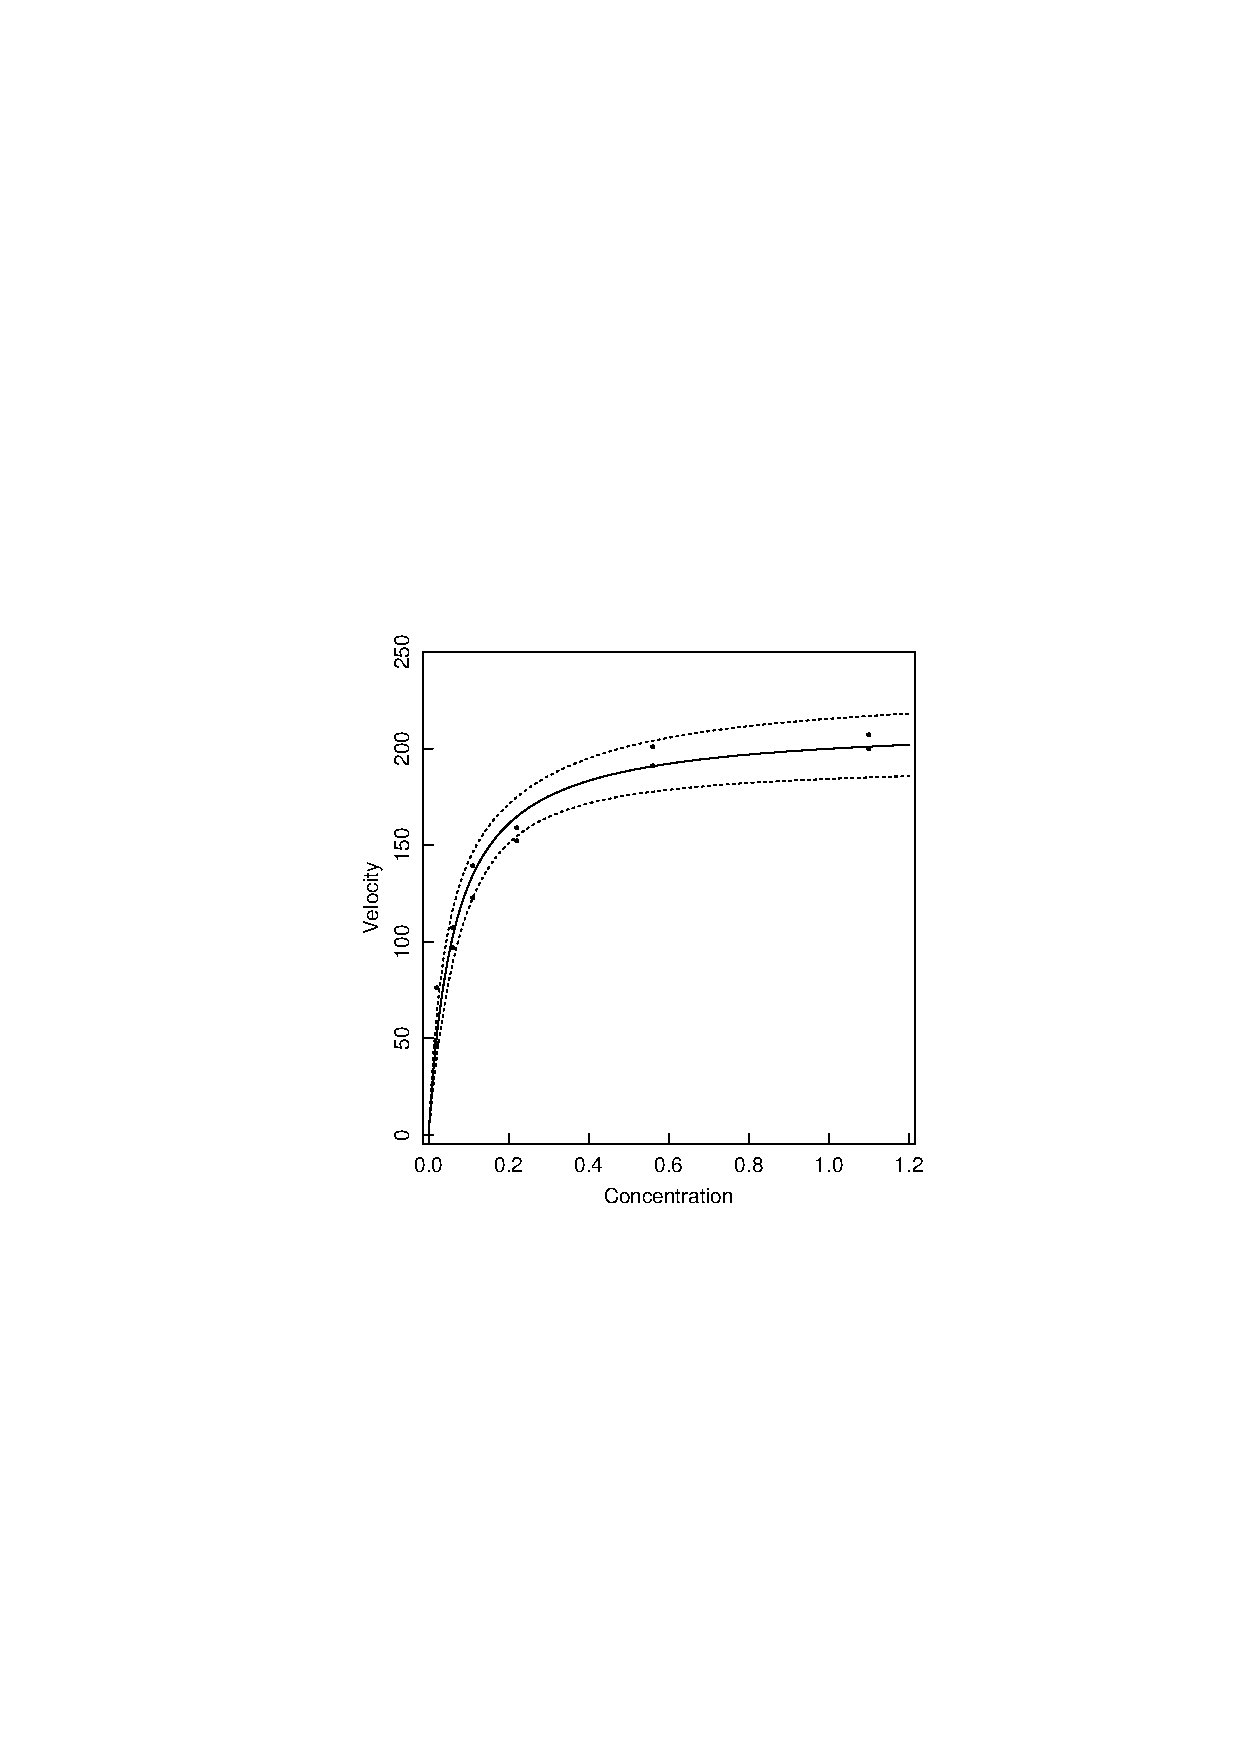
\includegraphics{2MICband}}%,width=\textwidth}}
    \caption{\label{fig:MICband}
    Approximate 95\% inference band for the Puromycin data.
    The fitted expectation function is shown as a solid line, and the 95\%
    inference band is shown as a pair of dotted lines.
    }
  \end{figure}
\end{example}

\begin{example}\label{bod:3}

The estimated response function for the BOD data
and the approximate 95\% inference band is plotted in
Figure \ref{fig:BODband}.
  \begin{figure}
    \centerline{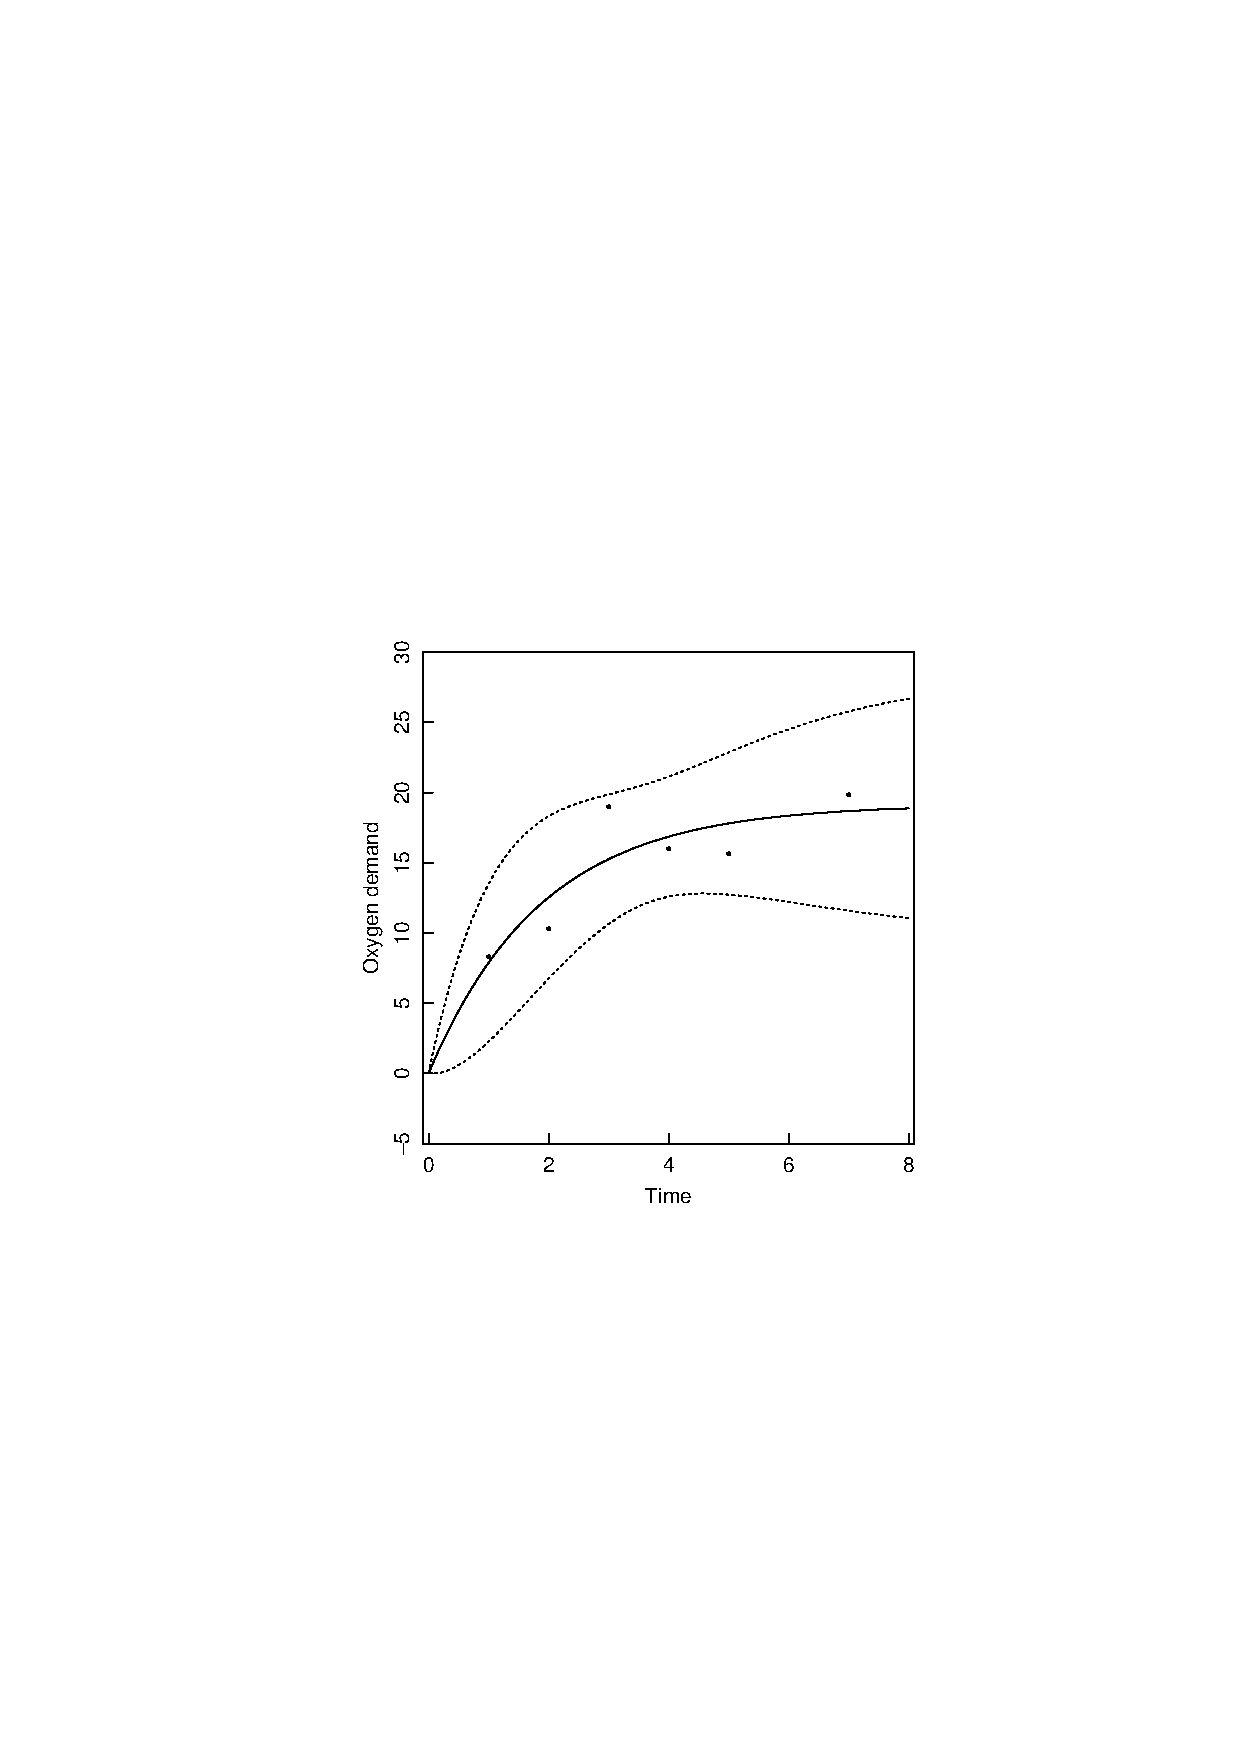
\includegraphics{2BODband}}%,width=\textwidth}}
    \caption{\label{fig:BODband}
    Approximate 95\% inference band for the BOD data.
    The fitted expectation function is shown as a solid line, and the 95\%
    inference band is shown as a pair of dotted lines.
    }
  \end{figure}
The band widens from zero width at $x=0$, narrows around $x=4$ and
then gradually approaches a constant width as $x\to\infty$.
\end{example}

Inference bands for nonlinear models behave quite
differently from those for linear models.
In the above examples,
because the functions are constrained to go through the
origin, the bands reduce to 0 there.
Also, because the model functions approach horizontal asymptotes,
the inference bands approach asymptotes.
These characteristics differ from those of the inference bands
for linear models as exemplified in Figure 1.3.
There it is seen that the bands are narrowest near the middle of
the data, and expand without limit.

\section{Nonlinear Least Squares via Sums of Squares}
\index{nonlinear!least squares via sums of squares}

Sums of squares occur explicitly in linear and nonlinear least
squares because of the assumptions of normality, independence,
and constant variance of the disturbances.
It is therefore natural to view linear and nonlinear regression
via sums of squares, which can help in understanding these two
topics.
The likelihood approach is especially closely linked to sum of
\index{likelihood}
squares contours, because the loglikelihood function is directly
\index{loglikelihood!function}
proportional to the sum of squares function $S ( \btheta )$.
\index{sum of squares!function}

An important characteristic of linear models is that the sum of
squares function $S ( \bbeta $) is quadratic.
Because of this, contours of constant sums of squares are
well-behaved regular curves or surfaces, such as ellipses and
ellipsoids, and so the loglikelihood function can be completely
summarized by:
  \begin{itemize}
    \item the minimum value of the sum of squares function,
          $S ( \hat{\bbeta} )$,
    \item the location of the minimum of the sum of squares function,
          $ \hat{\bbeta} $, and 
    \item the second derivative (Hessian) of the sum of squares
          \index{ Hessian "of sum of squares function"}
          function,
          \begin{displaymath}
            \frac{\partial^2 S ( \bbeta )}{\partial \bbeta \partial \bbeta
            \trans}= \bX \trans \bX    
          \end{displaymath}
  \end{itemize}
Furthermore, all these quantities can be
determined analytically.
For nonlinear models, however, the sum of squares function is not
regular or well behaved, and so it is difficult to summarize the
loglikelihood function.
\subsection{The Linear Approximation}
\index{linear approximation!to sum of squares function}

Linear approximations of the expectation function are used to
determine increments while seeking the least squares estimates,
and to determine approximate inference regions when convergence
has been achieved.
The linear approximation to $\boeta ( \btheta )$ based at $\btheta^0$,
(\ref{eqn:2.5}), produces a linear approximation to the
residual vector $\bz ( \btheta )$, (\ref{eqn:2.5a}), and hence a
\emph{quadratic} approximation $ \tilde S ( \btheta )$ to the sum of
squares function $S(\btheta)$, since
  \begin{eqnarray}\label{eqn:quada}
        S(\btheta)&=&\norm \by - \boeta ( \btheta ) \norm^2\\
        &=&\bz ( \btheta ) \trans  \bz ( \btheta )  \approx
        \tilde S(\btheta)\nonumber\\
        &=&[\bz^0-\bV^0(\btheta-\btheta^0)]\trans
        [\bz^0-\bV^0(\btheta-\btheta^0)]\nonumber\\
        &=&{\bz^0}\trans\bz^0-2{ \bz^0 } \trans \bV^0 ( \btheta -
        \btheta^0 ) + ( \btheta - \btheta^0 ) \trans { \bV^0 } \trans
        \bV^0 ( \btheta - \btheta^0 )\nonumber\\
        &=&S(\btheta^0)-2[\by-\boeta(\btheta^0)]\trans \bV^0
        ( \btheta - \btheta^0 )
        + ( \btheta - \btheta^0 ) \trans { \bV^0 } \trans \bV^0
        ( \btheta - \btheta^0 )
  \end{eqnarray}
The location of the minimum of $\tilde S ( \btheta )$ is
  \begin{displaymath}
    \btheta^1 = \btheta^0 +
( {\bV^0} \trans \bV^0 )^-1 { \bV^0 } \trans \bz^0
  \end{displaymath}
which gives the Gauss--Newton increment.

Note that the quadratic approximation (\ref{eqn:quada}) is
not the second order Taylor series approximation to $S ( \btheta )$
based at $\btheta^0$.
The Hessian in the Taylor series approximation includes
a term involving the second order partial derivatives of the
model function with respect to the parameters (see Section 3.5.1).

Contours of the approximate sum of squares function
\index{sum of squares!contour}
\index{contour!sum of squares}
(\ref{eqn:quada}) are ellipsoids centered at $\btheta^1$ and of
the form
  \begin{displaymath}
    ( \btheta - \btheta^1 ) \trans { \bV^0 } \trans \bV^0
( \btheta - \btheta^1 ) = c
  \end{displaymath}
Of particular interest is the approximating contour
  \begin{displaymath}
    ( \btheta - \btheta^1 ) \trans { \bV^0 } \trans \bV^0
( \btheta - \btheta^1 ) = {\bz^0} \trans
\bV^0 ( {\bV^0} \trans \bV^0 )^{-1} {\bV^0} \trans \bz^0
  \end{displaymath}
which passes through $\btheta^0$.
If this contour is close to the actual sum of squares contour
which passes through $\btheta^0$, then we can expect that
$\btheta^1$ will be close to the optimal value of $\btheta$.
\label{rum:sumsq}
\begin{example}
  \begin{figure}
    \centerline{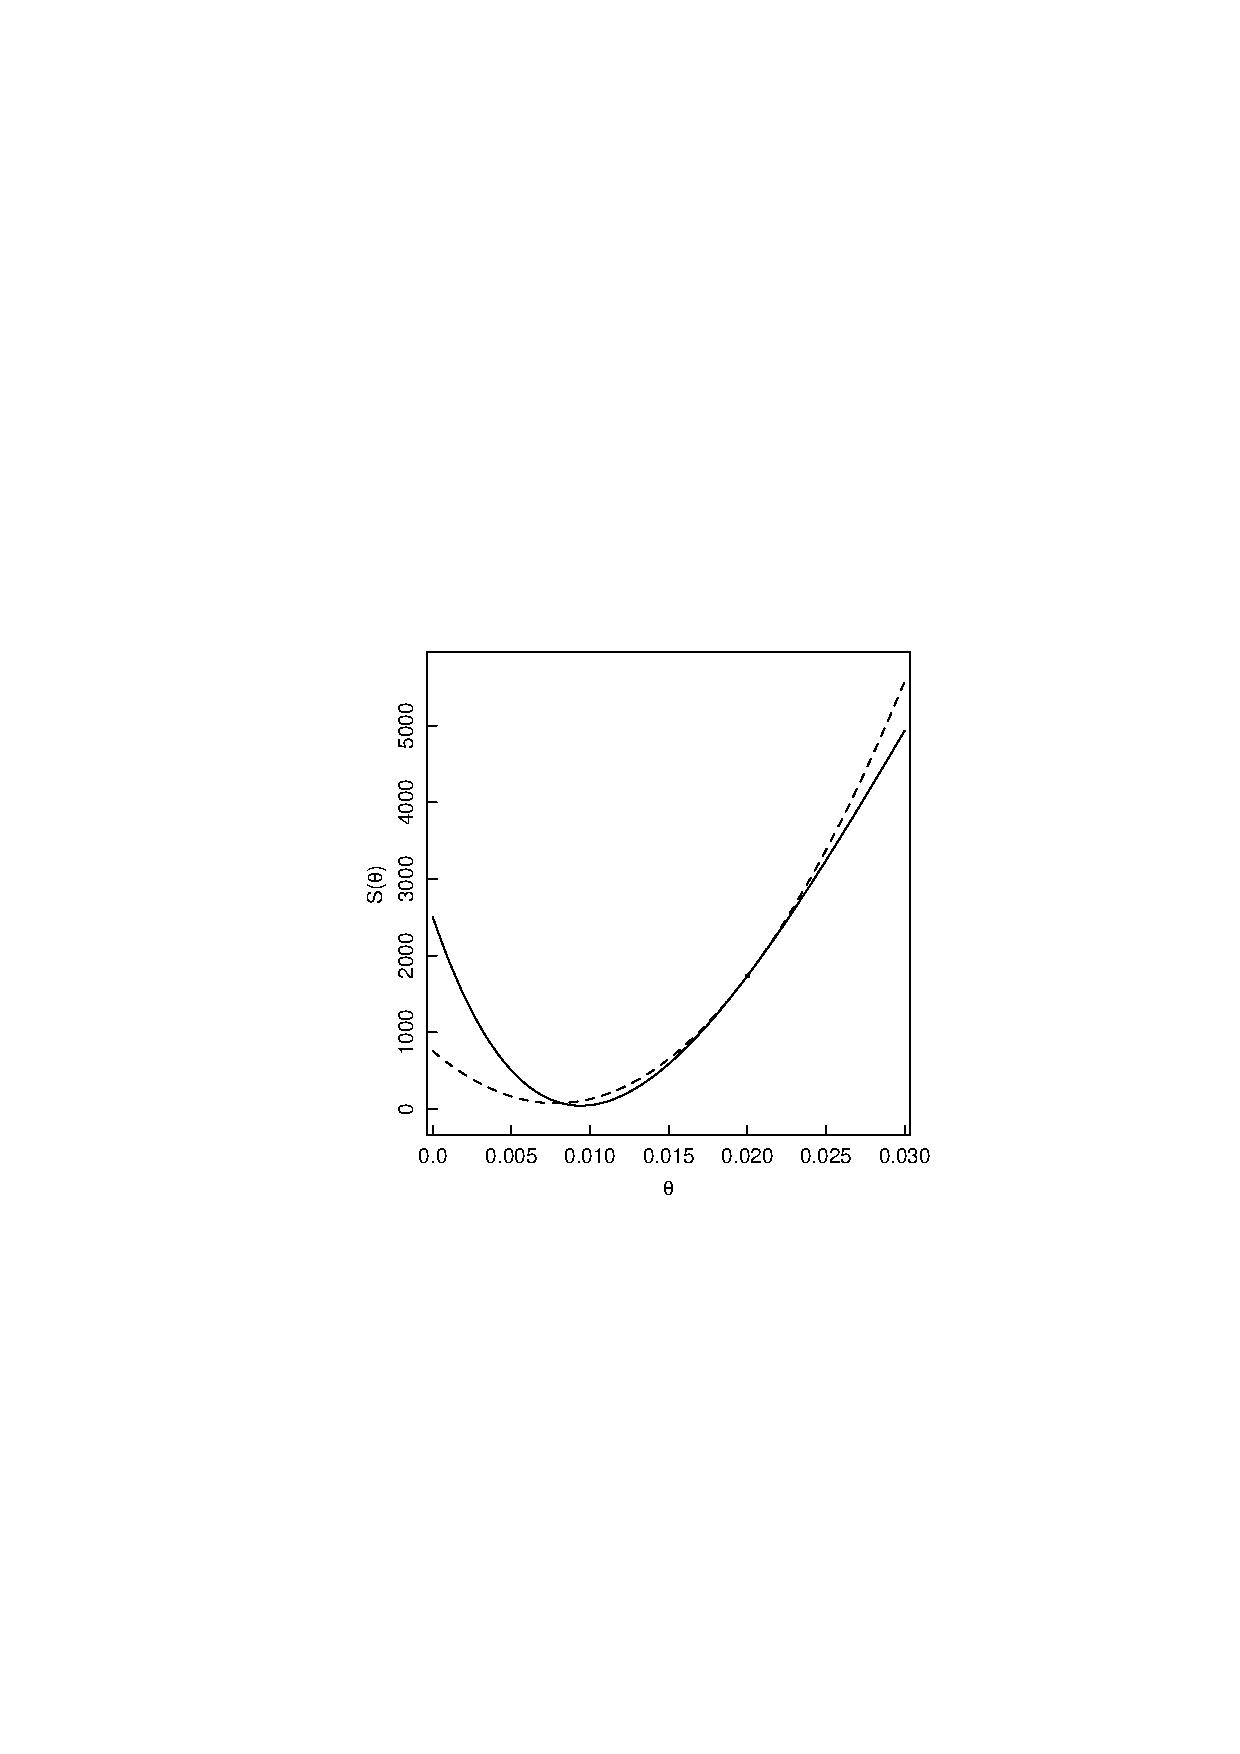
\includegraphics{2RUMsumsq}}%,width=\textwidth}}
    \caption[Sum of squares function for the Rumford data.]{
    \label{fig:RUMsumsq}
    Sum of squares function for the Rumford data.
    The true sum of squares curve is shown as a solid line, and the
    parabola from the linear approximation at $\theta^0=0.02$ is
    shown as a dashed line.
    }
  \end{figure}
In Figure \ref{fig:RUMsumsq} we plot the sum of squares function,
$S ( \theta )$, for the Rumford data as a solid line.
Superimposed on the plot is the approximating quadratic,
$\tilde S ( \theta )$, obtained by taking a linear Taylor
series approximation to the expectation function at
$\theta^0 = 0.02$, shown as a dashed line.

A careful examination of $S ( \theta )$ shows that it is not a parabola
but is asymmetric, with a steeper rise to the left of the
minimum than to the right.
The closeness of $S ( \theta )$ to a parabola indicates the small
degree of nonlinearity of this model--data set combination.
\index{nonlinearity!of model-data set}
The minimum of the approximating parabola is at
0.008, and so the Gauss--Newton increment is $0.008-0.02=-0.012$.
\end{example}
\label{mic:micSinc}
\begin{example}

In Figure \ref{fig:MICsumsqinc} we plot sum of squares contours,
  \begin{figure}
    \centerline{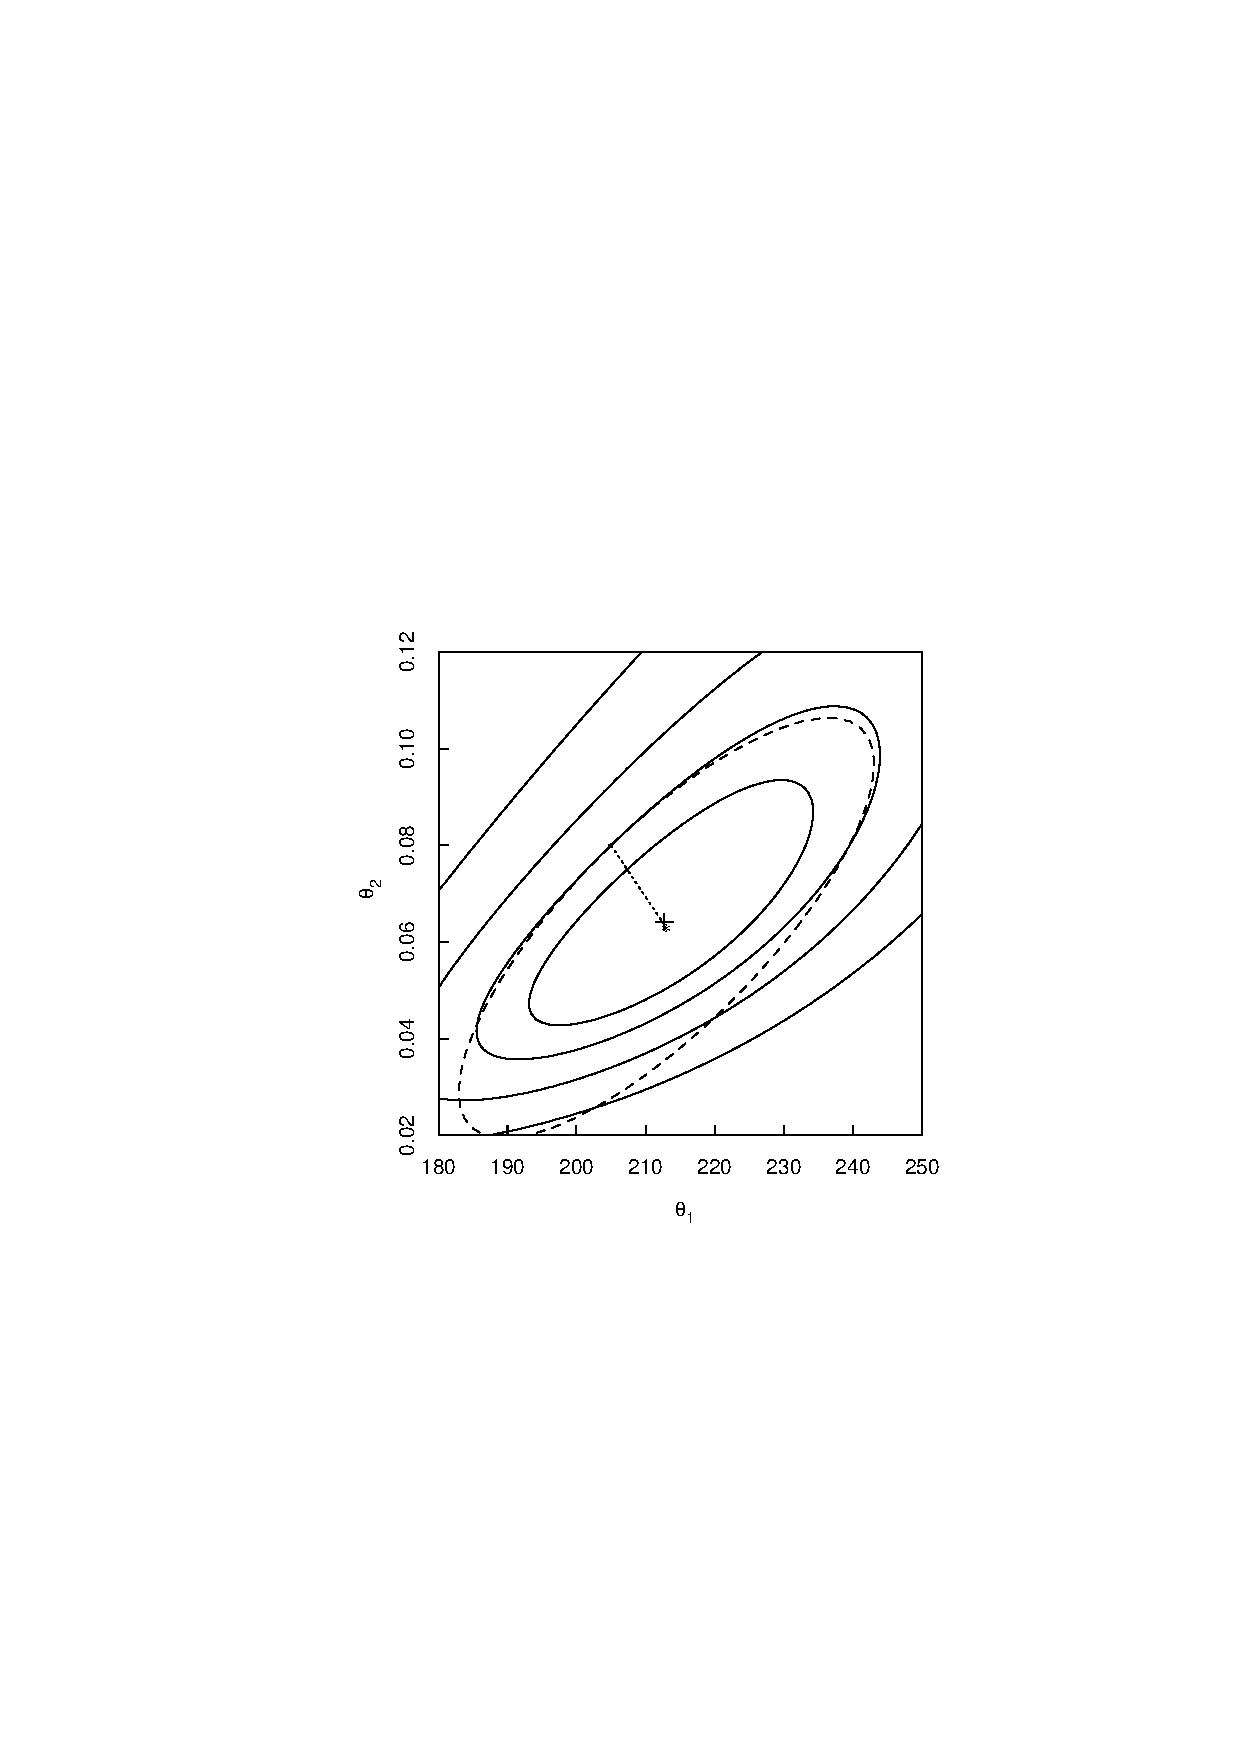
\includegraphics{2MICsumsqinc}}%,width=\textwidth}}
    \caption[Sum of squares contours for Puromycin data]{
    \label{fig:MICsumsqinc}
    Sum of squares contours for the Puromycin data.
    True sum of squares contours are shown as solid lines, and the
    elliptical approximate contour from the linear approximation at
    $\btheta^0=(205,0.08)\trans$ is shown as a dashed line.
    The location of the minimum sum of squares ($+$) and the center of the
    ellipse ($*$) are also shown.
    The dotted line is the Gauss--Newton increment.
    }
  \end{figure}
$S ( \btheta )$, for the Puromycin data, shown as solid lines, and the
location of the minimum, shown as $+$.
Also shown, as a dashed line, is the ellipse derived from the linear
approximation to the expectation function at
$\btheta^0 = ( 205 ,0.08 ) \trans$.
The approximating paraboloid has the
same value and curvature at $\btheta^0$ as the true sum of squares
surface, and so the location of the minimum of the paraboloid,
denoted by $*$,
is used as the apparent minimum of the true sum
of squares surface.
The Gauss increment is therefore the vector joining the starting
point $\btheta^0$ to the point indicated by $*$.

Because the model--data set combination is not badly nonlinear,
the sums of squares contours are quite elliptical, and the
minimum of the approximating paraboloid is near the minimum of
the true sum of squares surface.
\end{example}
\label{bod:BODsumsq}
\begin{example}
  \begin{figure}
    \centerline{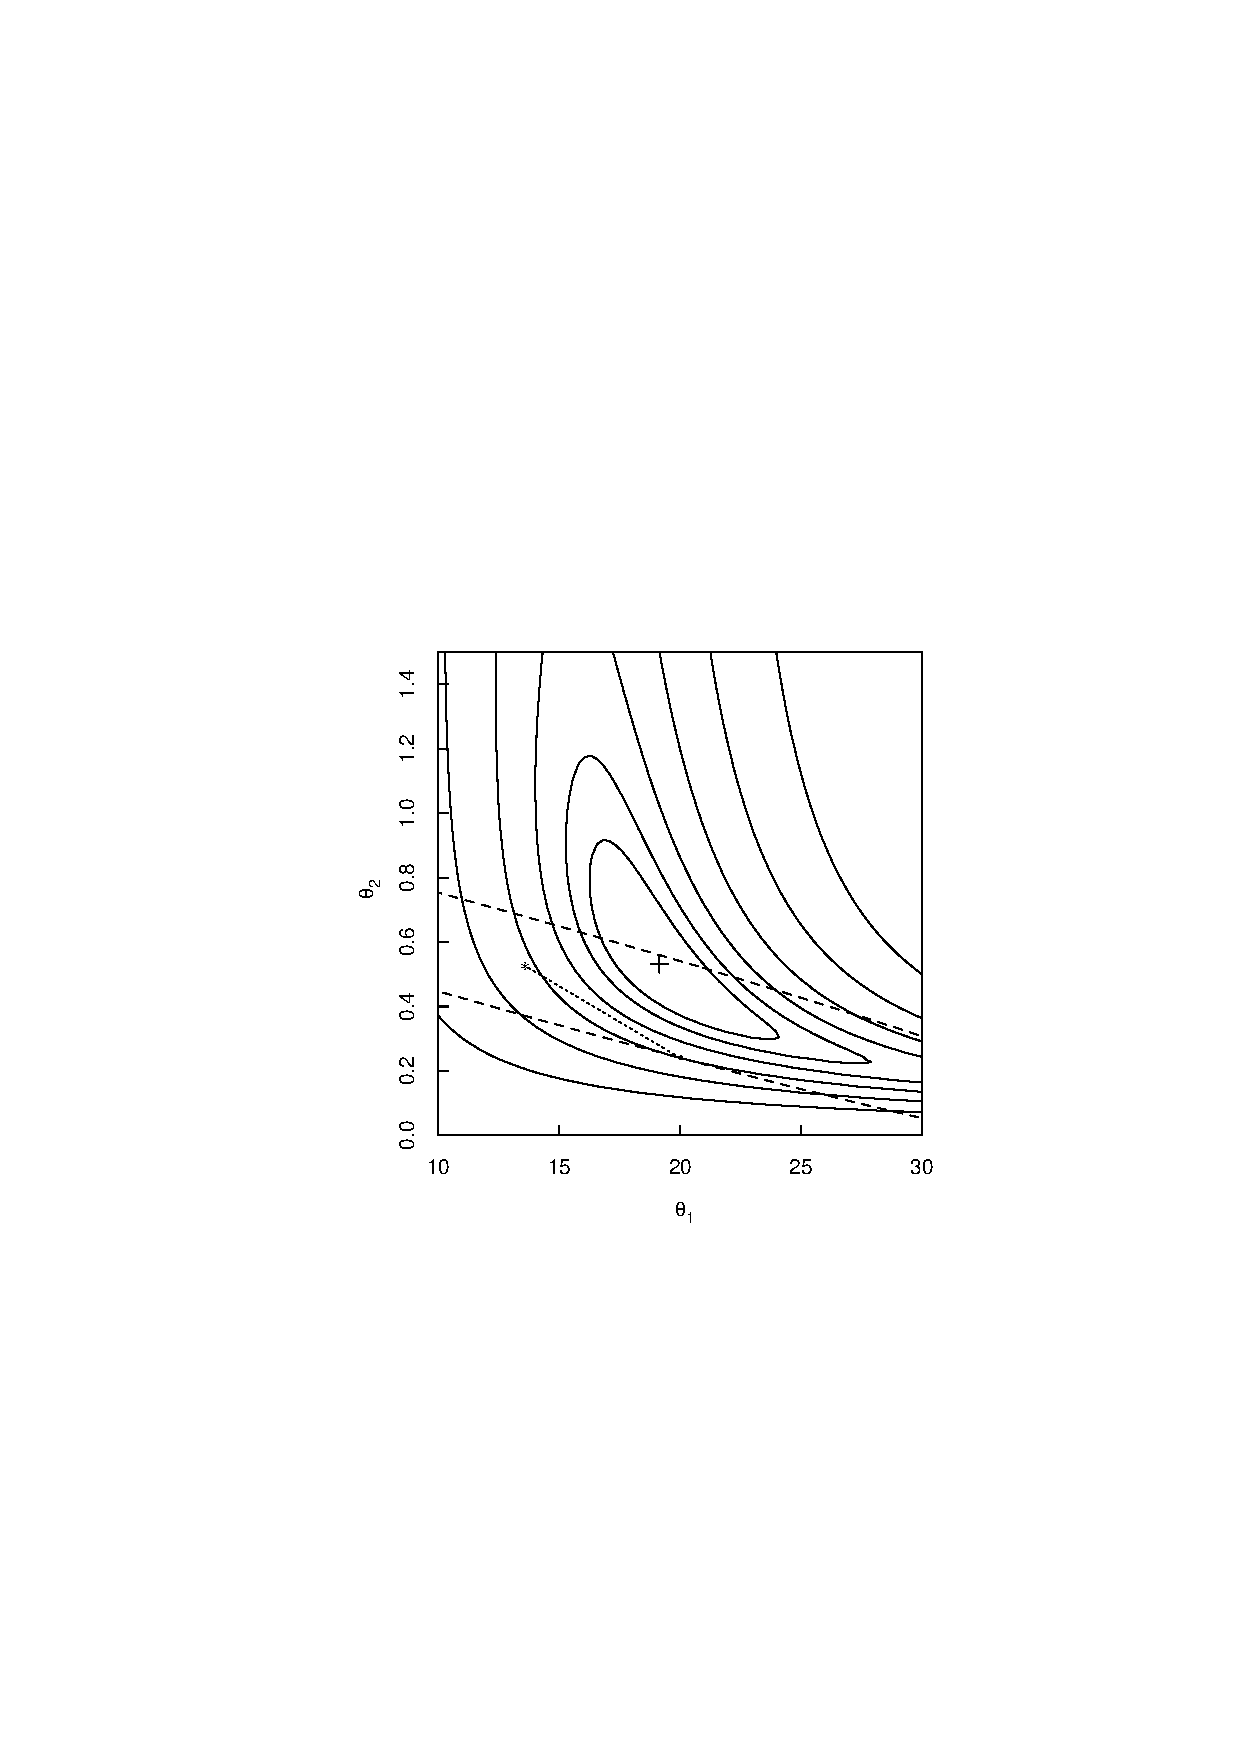
\includegraphics{2BODsumsq}}%,width=\textwidth}}
    \caption[Sum of squares contours for BOD data.]{
    \label{fig:BODsumsq}
    Sum of squares contours for the BOD data.
    True sum of squares contours are shown as solid lines, and a portion of
    the elliptical approximate contour from the linear approximation at
    $\btheta^0=( 20 ,0.24 ) \trans$ is shown as a dashed line.
    The location of the minimum sum of squares ($+$) and the center of the
    ellipse ($*$) are also shown.
    The dotted line is the Gauss--Newton increment.
    }
  \end{figure}
In Figure \ref{fig:BODsumsq} we plot sum of squares contours,
$S ( \btheta )$, for the BOD data, shown as solid lines, and
location of the minimum, shown as $+$.
Also shown, as a dashed line, is a portion of the ellipse derived from
the linear approximation to the expectation function at
$\btheta^0 = ( 20 ,0.24 ) \trans$.
The center of the ellipse is indicated by $*$.

In this example, the ellipse is a poor approximation to the true
contour.
\index{ellipse!approximation to sum of squares contour}
The center of the ellipse is not close to the minimum of the true
sum of squares surface and
furthermore has a true sum of squares greater than that at $\btheta^0$.
\end{example}
\subsection{Overshoot}
\index{overshoot}

The next iteration is carried out from the location of the
apparent minimum of the sum of squares surface---provided, of
course, that $S ( \btheta^1 )$ is less than
$S ( \btheta^0 )$.
In the Rumford example and in the Puromycin example,
because the nonlinearity is moderate,
the sum of squares at $\btheta^1$ is less
than that at $\btheta^0$, and so we can proceed to iterate
from $\btheta^1$.
For the BOD example, however, the sum of squares at
$\btheta^1$ is greater than that at
$\btheta^0$, so we have overshot the
minimum.
By incorporating a step factor, so that only a fraction of the increment
\index{step factor}
is used, we can find
a point with a smaller sum of squares, as described in Section 2.2.1.

\begin{problems}
  \prob
  Write a computer routine in a language of your choice to
  perform nonlinear least squares using the Gauss--Newton approach.
  Take the function, its derivatives with respect to the
  parameters, and starting values as input to the routine.
  If necessary, use the pseudocode in Appendix 3, Section A3.1
  for guidance.

  \prob
  Use a nonlinear least squares routine to fit a model of the form
  $\beta_1+\beta_2(\mbox{\rm age})^{\alpha}$ to the $\ln(\mbox{\rm PCB})$ data.
  Use starting values of $(-2.4,2.3,0.33)\trans$ (the least squares
  estimates for $\beta_1 ,\beta_{2}$ for $\alpha=0.33$ from
  Example PCB 2).

  \prob
  \subprob
  Plot the expectation surface for the Rumford model,
  using the design $\bx = ( 7,  28 ) \trans$.
  Mark the points on the expectation surface
  corresponding to the values
  $\theta=0,0.01,\ldots,0.1,0.2,\ldots,1.0,\infty$.
  Compare this expectation surface with the one based on
  the design $\bx = ( 4,  41 ) \trans$ plotted in Figure 2.3.
  Which design has smaller overall intrinsic nonlinearity?
  Which design has smaller overall parameter effects
  nonlinearity?
  
  \subprob                
  Plot the expectation surface for the Rumford model,
  using the design $\bx = ( 12,  14 ) \trans$.
  Mark the points on the expectation surface
  corresponding to the values
  $\theta=0,0.01,\ldots,0.1,0.2,\ldots,1.0,\infty$.
  Compare this expectation surface with the one based on
  the design $\bx=(4,41)\trans$ plotted in Figure 2.3 and
  with that from part (a).
  Which design has smallest overall intrinsic nonlinearity?
  Which design has smallest overall parameter effects
  nonlinearity?

  \subprob
  What kind of design would have zero intrinsic nonlinearity
  everywhere?  Why?

  \subprob
  Would the design in part (c) have zero parameter
  effects nonlinearity?  Why?

  \prob
  \subprob
  Plot the expectation surface for the linear model
  $\ln(\mbox{\rm PCB})=\beta\ln(\mbox{\rm age})$ for the design
  $\mbox{\rm age}=5,10$.
  Mark the points on the surface corresponding to
  $\beta=0,1,2,3$.

  \subprob
  Compare this expectation surface and its properties
  with those of the nonlinear Rumford model shown in
  Figure 2.3.

  \subprob
  Compare this expectation surface and its properties
  with those of the nonlinear Rumford model plotted in
  Problem 2.3.

  \prob
  \subprob
  Generate the expectation vector, the residual vector,
  the sum of squares  $S ( \btheta^0 )$, and the
  derivative matrix $\bV^{0}$ for the data and model
  from Appendix 4, Section A4.1, at the starting values
  $\btheta^0 = ( 2.20, 0.26 ) \trans$.

  \subprob
  Calculate the increment $\bdelta^0$ and
  $S(\btheta^1)$, where
  $\btheta^1=\btheta^0+\lambda\bdelta^{0}$, for
  $\lambda=0.25,0.50$, and $1.0$.
  Is a step factor less than 1 necessary in this case?

  \prob
  \subprob
  Use the fact that, for the model in Problem 2.5,
  $\theta_{1}$ is conditionally linear, and generate and
  plot exact sum of squares contours for the data in
  Appendix 4, Section A4.1.
  (That is, for any specified value of $\theta_{2}$, it
  is possible to use linear least squares to obtain the
  conditional estimate $\tilde \theta_{1}$ and to
  calculate the values of $\theta_{1}$ which produce a
  specified sum of squares.
  By specifying the sum of squares to be that
  corresponding to a contour value, it is possible to
  generate the exact coordinates of points on the contour.)
  Let $\theta_{2}$ go from 0.12 to 0.3 in steps of 0.01,
  and use contour values corresponding to 50, 75, and
  95\% confidence levels.
  Mark the location of the minimum on the plot.

  \subprob
  Compare these contours with those in Figure 2.23.
  Which data set suffers most from nonlinearity?

  \subprob
  Since the data are from the same type of experiment
  with the same model, how can this difference be
  explained?

  \prob
  Plot the point corresponding to $\btheta^{0}$ and the
  increment $\bdelta^{0}$ from Problem 2.5 on the contour plot
  from Problem 2.6.
  Mark the points corresponding to the values
  $\lambda=0.25,0.5$, and 0.75 on the increment vector.
  Is a step factor less than 1 necessary in this case?

  \prob
  \subprob
  Use the data, model, and starting values from Problem
  2.5 in a nonlinear estimation routine to obtain the
  least squares parameter estimates.

  \subprob
  Calculate and plot the linear approximation joint and
  marginal inference regions on the plot from Problem
  2.6.

  \subprob
  Are the linear approximation inference regions
  accurate in this case?

\end{problems}

% Local Variables: 
% mode: latex
% TeX-master: "nraia2"
% End: 

\chapter[Practical Considerations]{Practical Considerations in
Nonlinear Regression}

\index{practical considerations!in nonlinear regression}
\index{nonlinear!regression, practical considerations"}
\prologue{Rationally, let it be said in a whisper, experience is
certainly worth more than theory.}{Amerigo Vespucci}

Nonlinear estimation, like all data analysis procedures, involves
many practical considerations.
In this chapter, we discuss some
techniques which help ensure a successful nonlinear analysis.
The topics include model specification,
preliminary analysis,
determination of starting values,
transformations of parameters and variables,
other iteration schemes,
convergence,
assessment of fit and modification of models,
correlated residuals,
accumulated data,
comparison of models,
parameters as functions of other variables,
and
presentation of results.
A case study in which we illustrate many of the techniques presented
in this chapter is given in Section 3.13.
The important practical problem of designing experiments for nonlinear
models is discussed in the final section.
\section{Model Specification}
\index{practical considerations!model specification}
\index{model!specification in nonlinear regression}

An important step in any nonlinear analysis is specification of
the model, which includes specifying both the expectation function and the
characteristics of the disturbance.
\subsection{The Expectation Function}

Ideally, physical, biological, chemical, or other theoretical
considerations will lead to a \emph{mechanistic} model for the
expectation function.
The analyst's job is then to find the simplest form of the
model and the parameter estimates which provide an adequate fit of
the model to the data, subject to the assumptions about the
disturbance.
Note that it is not necessary for the expectation function to be
stated as an explicit function of the parameters and the control
variables.
In Chapter 5 we discuss an important class of models, known as
compartment models, in which the expected response is given by
the solution to a set of linear differential equations.
Special techniques, developed in that chapter, can be used to
avoid solving explicitly for the expectation function in terms of
the parameters and independent variables.

In other situations, the expectation function may be the solution to a
nonlinear differential equation or an
\index{differential equation!specification of nonlinear model}
integral equation which has no analytic solution.
Then the value of the expectation function must be determined
numerically for any given parameter values for a regular
nonlinear least squares program to be used.
In such situations, numerical parameter derivatives or a
derivative-free optimization procedure will often have to be used
to calculate the least squares estimates.
However, as discussed in \citeasnoun{cara:stew:1985}, when an expectation function
%\glossary{ Caracotsios, M.}
%\glossary{ Stewart, W.E.}
is obtained from the solution to a set of ordinary differential
equations, the parameter derivatives of the expectation function
can be determined from the sensitivity functions for the
system of differential equations.
These functions are evaluated numerically at the same time
as the solution of the differential equations is evaluated.

\begin{example}\label{pin:nonlin}

The decomposition of $\alpha$-pinene was investigated by
\nocite{fugu:hawk:1945,fugu:hawk:1947}
Fuguitt and Hawkins (1945, 1947), who reported
%\glossary{ Fuguitt, R.E.}
%\glossary{ Hawkins, J.E.}
the concentrations of five reactants as a function of time,
at a series of reaction temperatures.
In Appendix A, Section~\ref{atbl:pin}, we present the data for the run at
189.5$^\circ$C.

We discuss these data in Chapters 4 and 5 and fit a model
which is specified by a set of linear differential equations.
As discussed in Chapter 5, the parameters in such models can be
estimated very easily, due to the ease with which they can be specified
and the ease with which the responses and the derivatives with respect
to the parameters can be evaluated.
As will be also shown in Chapter 5, however, the linear differential
equation model does not provide an adequate fit to the $\alpha$-pinene
data.

\citeasnoun{stew:soer:1981} analyzed the complete data set
%\glossary{ Stewart, W.E.}
%\glossary{ Soerensen, J.P.}
reported by \nocite{fugu:hawk:1945,fugu:hawk:1947}
Fuguitt and Hawkins (1945, 1947), and
%\glossary{ Fuguitt, R.E.}
%\glossary{ Hawkins, J.E.}
proposed a model consisting of a set of five nonlinear differential
equations
  \begin{eqnarray*}
    \frac{df_1}{dt}&=&-( \theta_1+\theta_2) f_1 -2 \theta_3 f_1^2\\
    \frac{df_2}{dt}&=&- \theta_4 f_2 + \theta_5 f_4\\
    \frac{df_3}{dt}& =& \theta_1 f_1\\
    \frac{df_4}{dt}&=&\theta_2 f_1 + \theta_4 f_2 -\theta_5 f_4 -2
    \theta_6 f_4^2 +2 \theta_7 f_5\\
    \frac{df_5}{dt}&=& \theta_8 f_1^2 +\theta_6 f_4^2-\theta_7 f_5
  \end{eqnarray*}
where $f_i ,i=1 ,\ldots,5$, represent the theoretical responses
at time $t$.

There is no analytic solution to this set of differential
equations, and so we must use numerical procedures.
For given values of
$\btheta=( \theta_1 ,\ldots,\theta_8 ) \trans$,
the differential equations would be integrated numerically using,
say, a Runge--Kutta integration routine \cite{cont:debo:1980}.
%\glossary{ Conte, S.D.}
%\glossary{ deBoor, C.}
The numerical estimates of the responses, ${\bf f} ( t )$, and the
observed responses $\by ( t )$,
at the observation times, could then be used to
calculate residuals from which an appropriate estimation criterion
can be evaluated.

We discuss the choice of estimation criterion for multiresponse data
in Chapter 4.
Methods for obtaining derivatives of the response functions at
the observation times by means of the
``sensitivity functions''
      \begin{displaymath}
        \frac{\partial f_i(t)}{\partial\theta_p}\quad
        i=1,\ldots,5\quad p = 1 ,\ldots, P 
      \end{displaymath}
are given in \citeasnoun{cara:stew:1985}.
%\glossary{ Caracotsios, M.}
%\glossary{ Stewart, W.E.}
The derivative matrix $\bV$ can then be calculated from the
sensitivity functions.
\end{example}

In other situations, a mechanistic model may not be advanced by
the researcher, in which case the statistician will be called
upon to suggest an equation.
One approach is to ask the researcher to search through the
literature to see if models have been proposed.
If not, the statistician and the researcher can apply their
modeling skills and develop a plausible mechanistic model.
Failing this, the statistician must formulate a model which has
the same sort of behavior as the data.
If the data rise monotonically to an asymptote, perhaps a
Michaelis--Menten, exponential rise, or logistic model might be
appropriate.
If the data peak and then decay towards zero, perhaps a
double exponential, a Michaelis--Menten model with a quadratic
term in the denominator, or a gamma function would be suitable.

Finally, if there are several sets of data, it may be possible to use
the self-modeling approach of \citeasnoun{lawt:sylv:magg:1972}.
%\glossary{ Lawton, W.H.}
%\glossary{ Sylvestre, A.}
%\glossary{ Maggio, M.S.}
This approach has been used in modeling spirometer curves
which give the volume of air expelled
from the lungs as a function of time for a number of subjects,
and in modeling the
creatine phosphokinase serum levels in patients suffering
myocardial infarctions \cite{arms:watt:hami:chio:park:1979}.
%\glossary{ Armstrong, P.W.}
%\glossary{ Watts, D.G.}
%\glossary{ Hamilton, D.C.}
%\glossary{ Chiong, M.A.}
%\glossary{ Parker, J.O.}

\subsection{The Disturbance Term}
\index{practical considerations!disturbance}
\index{disturbance!practical considerations}

All nonlinear estimation programs are based on specific
assumptions about the disturbance term, usually that the
disturbance is additive and normally distributed with zero mean,
constant variance, and independence between cases (see Section
1.3).
Checking assumptions on the disturbance term is considerably
easier and more sensitive
if the data include replications at some or all of the design
points.
It is helpful if the experimental runs have been randomized,
although many nonlinear experiments involve sequential
measurements of the response, so that randomization may not be
feasible.

At the initial stage, it is generally possible to check only one
of the assumptions on the disturbance, namely constancy of variance.
\index{variance!constant}
If there are replications, one can simply plot the data and look
\index{replication}
to see if the spread of the data tends to systematically increase
or decrease with respect to any of the predictor
variables.
Alternatively, one can use an analysis of variance program to
obtain averages and estimated variances and standard deviations for the
replicated responses and then plot the variances or standard deviations
versus the average, again looking for any
systematic relationship, as discussed in Section 1.3.
If none is apparent, then it may be tentatively assumed that the
variance is constant and the analysis can proceed;  if there is a
relationship, then oftentimes a simple power transformation such
as square root, logarithm, or inverse will stabilize the variance.
Even without replications, some visual indication of constancy of
variance can be gained from a data plot but this is
not as definitive as when replications are available.

Note that transforming the data also involves transforming the
expectation function.
Thus, if there is a well-justified expectation function for the
response but the data should be transformed to induce constant
variance, then the same transformation should be applied to the expectation
function to preserve the fundamental relationship.
(See Section 3.9 for an example.)
This is discussed more fully in \citeasnoun{carr:rupp:1984},
%\glossary{ Carroll, R.J.}
%\glossary{ Ruppert, D.}
where the Box--Cox transformations (Section 1.3.2)
%\glossary{ Box, G.E.P.}
%\glossary{ Cox, D.R.}
are applied to both the
observed responses and the expected responses using the same
transformation parameter $\lambda$.
The optimal value of $\lambda$ is determined by maximum likelihood.
Alternatively, one can use weighted least squares
\cite{drap:smit:1998} if a
%\glossary{ Draper, N.R.}
%\glossary{ Smith, H.}
reasonable decision can be made about how the
variance changes with respect to the response.

After a model has been fitted, it is possible to perform further
checks on the disturbance assumptions by examining the residuals,
as described in Sections 1.3, 3.7, and 3.8.
It is also possible to check adequacy of the model and to compare
rival models, as discussed in Section 3.10.

\section{Preliminary Analysis}
\index{practical considerations!preliminary analysis}

Having decided on a suitable expectation function (or set of
plausible expectation functions) and a transformation of the data (and the
expectation function, if necessary), we need to provide a
computer program with the expectation function in some form
and, unless numerical derivatives or derivative-free
methods are used, its derivatives with respect to the parameters.
Naturally, the expectation function and derivatives must be
\emph{correctly specified} and \emph{correctly coded}, but (as
most nonlinear analysts know from experience) a great many errors
occur at this stage.

One way to ensure that the function is correctly specified and
correctly coded is to use a separate program or even a calculator
to evaluate the function at one or two distinct design points then
compare these values with those from the nonlinear estimation routine.
The same technique can be used for the derivatives, of course,
but a better procedure is to compare the analytic
derivatives from the routine with numerical derivatives obtained
\index{derivative!numerical}
\index{derivative!of expectation function}
from finite differences of the expectation function (see Section 3.5.3).
These comparisons are done on the basis of the relative
differences between the derivatives calculated in the two ways.
If $v_{np}$ is the analytic derivative for case $n$ and
parameter $p$ while $\tilde v_{np}$ is the finite difference
approximation, then the relative difference is
\begin{displaymath}
  \begin{cases}
    \frac{| v_{np}-\tilde v_{np}|}{|v_{np}|} & v_{np} != 0\\
    |\tilde v_{np} | & v_{np} = 0
  \end{cases}
\end{displaymath}
Verifying that the relative differences are small
not only provides a check on the derivatives, but,
indirectly, a check on the expectation function, because a
discrepancy between the numerical derivatives and the analytic
derivatives can be due to either incorrect specification or
coding of the analytic derivatives, or due to incorrect
specification or coding of the expectation function, or both.

When coding the function, and especially when deriving and coding
the derivatives, it is good practice to use temporary variables
and the chain rule for derivatives, as demonstrated below.
This helps avoid algebraic errors, which can occur when trying to
reduce a function to its simplest form.

\label{iso:code}
\begin{example}
For the isomerization data of Example Isomerization 1, the function
      \begin{displaymath}
        f ( \bx , \btheta ) =\frac{\theta_1 \theta_3 ( x_2 - x_3 / 1.632 )
        }{1 + \theta_2 x_1+\theta_3 x_2 +\theta_4 x_3} 
      \end{displaymath}
is considered appropriate.
To code the function and its derivatives,
suppose the variables $x_1,x_2,x_3$ are coded as
\begin{verbatim}
X(1), X(2), X(3),
\end{verbatim}
and the parameters as
\begin{verbatim}
THETA(1), THETA(2), THETA(3),
\end{verbatim}
and
\begin{verbatim}
THETA(4).
\end{verbatim}
Then we can code the function simply and accurately by
introducing the temporary variables
\begin{verbatim}
NUMX  = X(2) - X(3)/1.632
DENOM = 1.0 + THETA(2)*X(1) + THETA(3)*X(2)
       + THETA(4)*X(3)
RATIO = NUMX/DENOM
\end{verbatim}
so the function becomes
\begin{verbatim}
F = THETA(1)*THETA(3)*RATIO
\end{verbatim}
Next, introducing the temporary variable
\begin{verbatim}
FD = - F/DENOM
\end{verbatim}
the derivatives become (denoting
$ \partial f / \partial \theta_1 $
by {\tt F1} and so on),
\begin{verbatim}
F1 = THETA(3)*RATIO
F2 = FD*X(1)
F3 = THETA(1)*RATIO + FD*X(2)
F4 = FD*X(3)
\end{verbatim}
\end{example}
It is also important to check that the data being analyzed are
valid.
That is, one must always ensure that the correct numerical values
of the response and predictor variables have been entered into the
machine.
Probably the most effective way to check this is to plot the
response versus each predictor variable, making sure that the
response behaves the way it should with respect to each of the
predictor variables.

\section{Starting Values}
\index{practical considerations!starting values}
\index{starting values}

One of the best things one can do to ensure a
successful nonlinear analysis is to obtain good starting values
for the parameters---values from which convergence is quickly obtained.

Several simple but useful principles for determining starting values
can be used:
\begin{enumerate}
  \item interpret the behavior of the expectation function in terms of
        the parameters analytically or graphically;
  \item interpret the behavior of derivatives of the expectation
        function in terms of the parameters analytically or graphically;
  \item transform the expectation function analytically or
        graphically to obtain simpler, preferably linear, behavior;
  \item reduce dimensions by substituting values for some
        parameters or by evaluating the function at specific design
        values; and
  \item use conditional linearity.
\end{enumerate}

We discuss each of these techniques in turn, and illustrate them
with specific examples.
For further discussion on obtaining starting values, see
\citeasnoun{ratk:1983}.
%\glossary{ Ratkowsky, D.A.}
\subsection{Interpreting the Expectation Function Behavior}
\index{starting values!interpreting expectation function}

One of the advantages of nonlinear regression is that the
parameters in the expectation function are usually meaningful to
the scientist or researcher.
This meaning can be graphical, physical, biological, chemical, or in
some other appropriate form, and can be very helpful in
determining starting values.
Initial estimates for some of the parameters may be available from
related experiments.
Also, plotting a nonlinear expectation function using various
values for the parameters
is an extremely beneficial exercise, because
in this way one becomes familiar with the function and how the parameters
affect its behavior.

Sometimes starting values can be obtained by considering the
behavior near the origin or at other special design values.
For example, letting $x = 0$ gives the initial value of $\theta_1 + \theta_{2}$ for the model
$f ( x , \btheta ) = \theta_1 + \theta_2 e^{{-} \theta_3 x}$, and letting $x  \to  \infty$ gives
the asymptote $\theta_{1}$ (assuming $\theta_3  0$).
\label{mic:start1}
\begin{example}

In the Michaelis--Menten expectation function, $f = \theta_1 x / ( \theta_2 + x )$, the parameter $\theta_{1}$ is the
asymptotic velocity of the enzymatic reaction, and so can be
estimated by the maximum observed data value, $y_{\mbox{\rm max}}$, or by
eye from a plot.
Graphically, $\theta_{1}$ represents the asymptotic value of $f$
as $x \to \infty$.
Similarly, $\theta_{2}$ represents the half-concentration,
i.e. the value of $x$ such that when the concentration reaches that
value the velocity is one-half its ultimate value.
For the Puromycin data, $y_{max} = 207$ provides a
good starting value for $\theta_{1}$.
From a plot of the data (Figure 2.1),
or simply from a listing, it can be seen
that the observed velocity reaches $y_{max} / 2$ at a
concentration of about 0.06 and so this value can be used as a
starting value for $\theta_{2}$.
\end{example}
\subsection{Interpreting Derivatives of the Expectation Function}
\index{starting values!interpreting derivatives of expectation function}

Sometimes rates of change of the function at specified design
values can be used to obtain parameter starting estimates.
For example, the derivative with respect to $x$ of the
Michaelis--Menten model at
$x = 0$ is $\theta_1 / \theta_{2}$, and so by estimating the
rate at $x = 0$ from the ratio of differences of adjacent $y$
values over differences of
adjacent $x$ values, and dividing this rate into $y_{max}$, we can obtain a starting value for $\theta_{2}$.
For Puromycin data, we obtain
$\theta_2 = 207/ ( 61/0.02 ) = 0.068$.

Similarly, derivatives at special values of $x$, such as limits or
points of inflection, can be used.
For example, for the double exponential model
\begin{displaymath}
  f = \theta_1 e^{ - \theta_2 x } + \theta_3 e^{ - \theta_4 x }
\end{displaymath}
assuming $\theta_2  \theta_{4}$,
the function behaves like a
simple exponential $\theta_3 e^{ - \theta_4 x }$ for
large $x$ and like
$\theta_3 + \theta_1 e^{ - \theta_2 x }$ for small $x$.
Thus, the rate of change at small $x$ provides an estimate of
$\theta_{2}$, and at large $x$ an estimate of $\theta_{4}$.
\subsection{Transforming the Expectation Function}
\index{starting values!transforming expectation function}

Transformations of the expectation function can often be used to obtain
starting values.
For instance, for the Michaelis--Menten model with a linear or
quadratic denominator, simply taking the reciprocal of the
function produces a model which can be rewritten as a linear
model.
\index{starting values!transformably linear model}
\index{transformably linear!model}
Linear least squares can be used on the reciprocal data to
estimate the linear parameters, which can then be used to obtain
starting values for $\btheta$.
The model from Example Isomerization 1,
\begin{displaymath}
  f ( \bx ,  \btheta ) = \frac{\theta_1 \theta_3
    ( x_2 - x_3 / 1.632)}{1 + \theta_2 x_1 + \theta_3 x_2 + \theta_4 x_3}
\end{displaymath}
is also transformably linear, since
\begin{displaymath}
  \frac{ x_2 - x_3 / 1.632 }{f(\bx,\btheta)}=\frac{1}{\theta_1 \theta_3} +
  \frac{\theta_2}{\theta_1 \theta_3 }  x_1 +
  \frac{1}{\theta_1}x_2+\frac{\theta_4}{\theta_1\theta_3} x_3
\end{displaymath}
A linear regression (with a constant term)
of $(x_2 - x_3 / 1.632) / y$ on $x_{1}$, $x_{2}$,
and $x_{3}$ would yield starting values
\begin{displaymath}
  \begin{aligned}
  \theta_1^0&=\frac{1}{\hat\beta_2}\\
  \theta_2^0&=\frac{\hat\beta_1}{\hat \beta_0}\\
  \theta_3^0&=\frac{\hat\beta_2}{\hat\beta_0}\\
  \theta_4^0 &= \frac{\hat\beta_3 }{\hat\beta_0}
  \end{aligned}
\end{displaymath}

For the model
$f(\bx,\btheta)=\exp [ - \theta_1 x_{1\exp} ( - \theta_2 / x_2 ) ]$,
used in a chemical kinetics example \cite[p.~124]{bard:1974},
%\glossary{ Bard, Y.}
taking logarithms twice gives
\begin{displaymath}
  \ln \ln f=\ln  x_1+\ln(-\theta_1)-\frac{\theta_2}{x_2}
\end{displaymath}
and one could again use linear least squares to obtain starting
values.

Graphical transformations are also very effective.
Plotting $f$ versus $x$ on semilog paper or plotting $\ln  f $ versus
$x$ on regular graph paper often reveals the true nature of
the data or enables one to
see when one portion of the model is dominant, and hence where one
can measure a rate and associate it with a particular parameter.

For example, the double exponential model
\begin{displaymath}
  f(x,\btheta)=\theta_1 e^{-\theta_2 x}+\theta_3  e^{-\theta_4 x}
\end{displaymath}
with $\theta_2  \theta_{4}$ is approximately
$\ln  f = \ln  \theta_3 - \theta_4 x$
at large $x$, which gives a
straight line on a semilog plot.
A simple fit can then be made by eye to obtain values for $\theta_{3}$ and $\theta_{4}$.
These values can then be used to calculate values of
$\theta_3 e^{ - \theta_4 x }$ at all values of $x$, and hence
residuals $\tilde y = y - \theta_3 e^{ - \theta_4 x }$ can
be derived.
Plotting $\tilde y$ versus $x$ on semilog paper then enables one to
estimate $\theta_{1}$ and $\theta_{2}$.
This process, known as \emph{peeling}, can be used when the
\index{peeling}
\index{starting values!peeling}
expectation function is a sum of several exponentials.
\label{sulf:peeling}
\begin{example}

To demonstrate the technique of peeling, we consider sulfisoxazole
data given in \citeasnoun{kapl:wein:abru:lewi:1972} and described
%\glossary{ Kaplan, S.A.}
%\glossary{ Weinfeld, R.E.}
%\glossary{ Abruzzo, C.W.}
%\glossary{ Lewis, M.}
in Appendix 1, Section~\ref{atbl:sulf}.
In this experiment, sulfisoxazole was administered
to a subject intravenously, blood samples were taken at specified times,
and the concentration of sulfisoxazole in the plasma was measured.
The data are plotted in Figure~\ref{fig:SULFdata}.
\begin{figure}
  \centerline{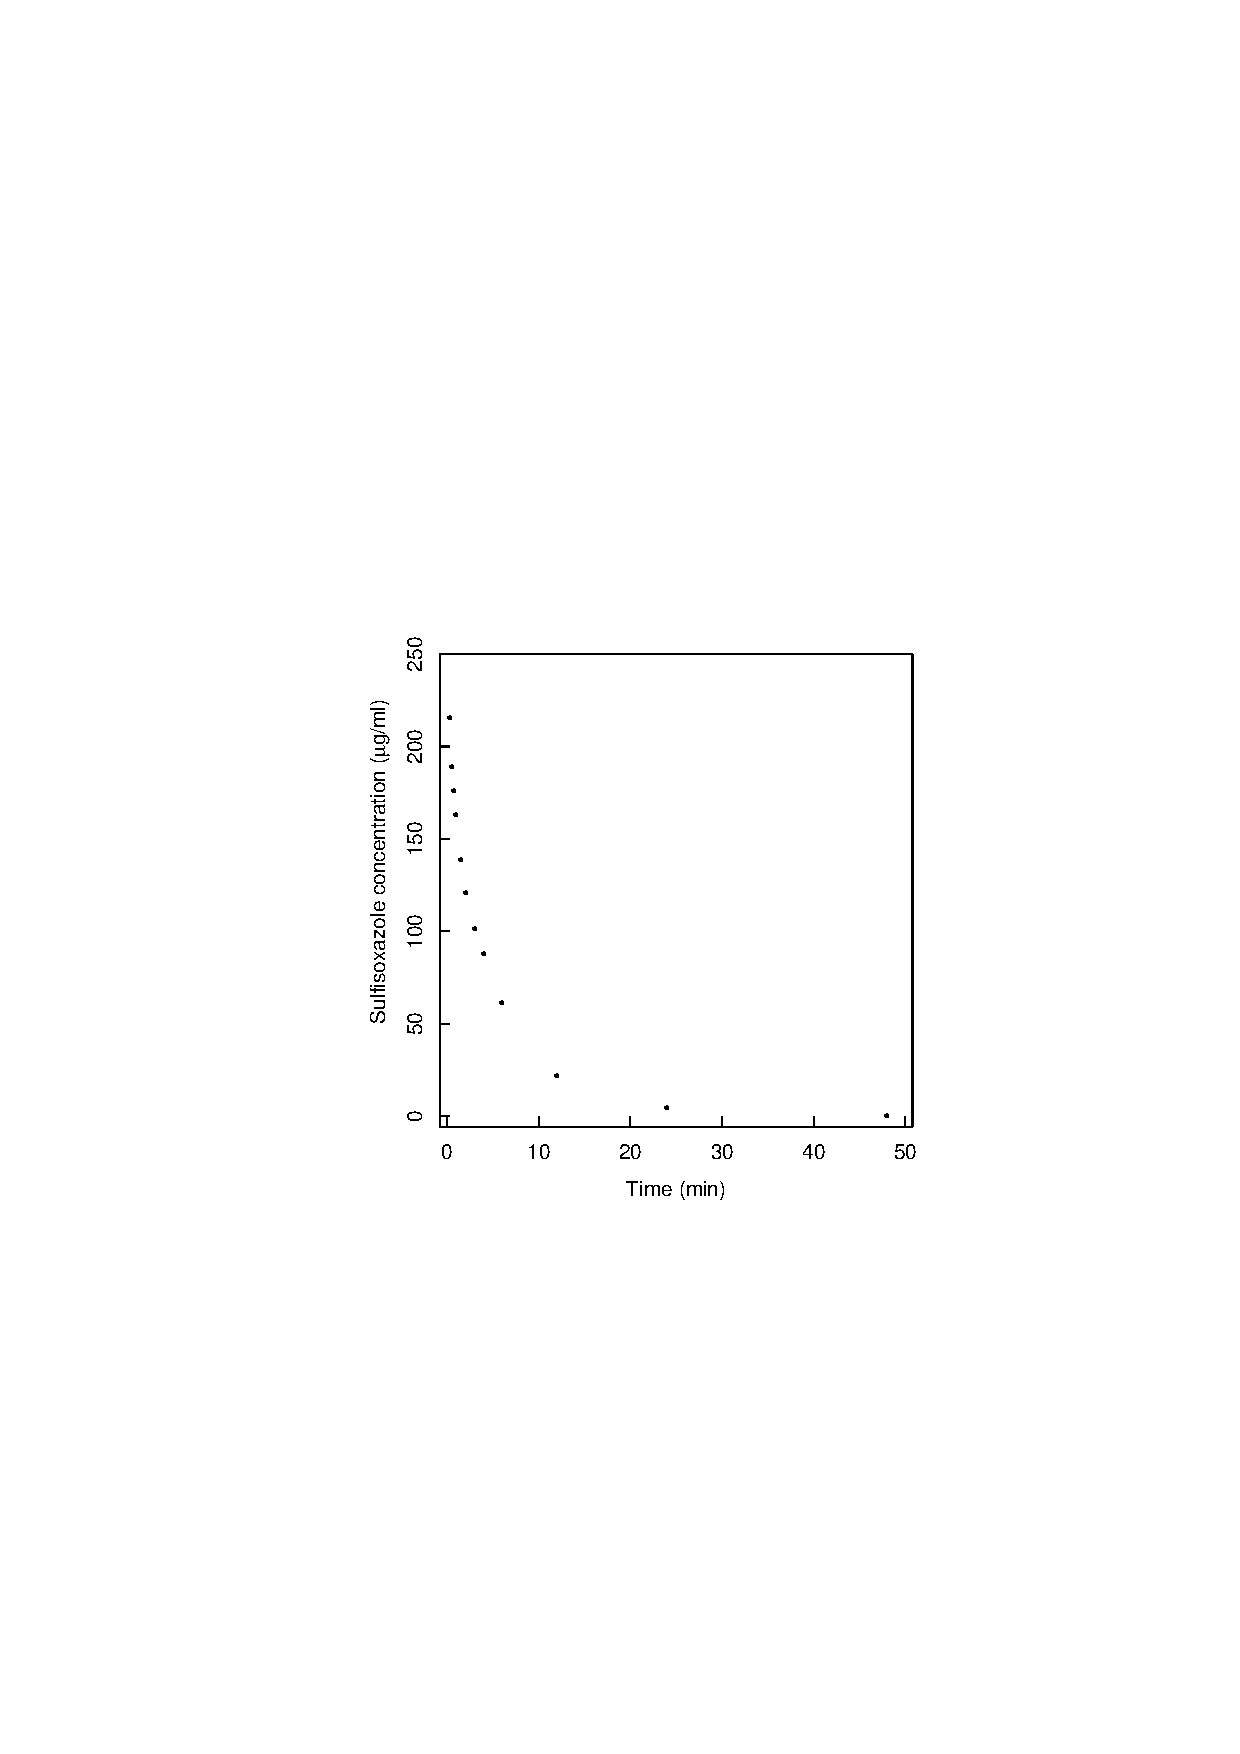
\includegraphics{3SULFdata}}
  \caption{\label{fig:SULFdata}
    Plot of sulfisoxazole concentration in plasma versus time.}
\end{figure}

Plotting the sulfisoxazole concentration on a log scale versus $x$ as
\begin{figure}
  \centerline{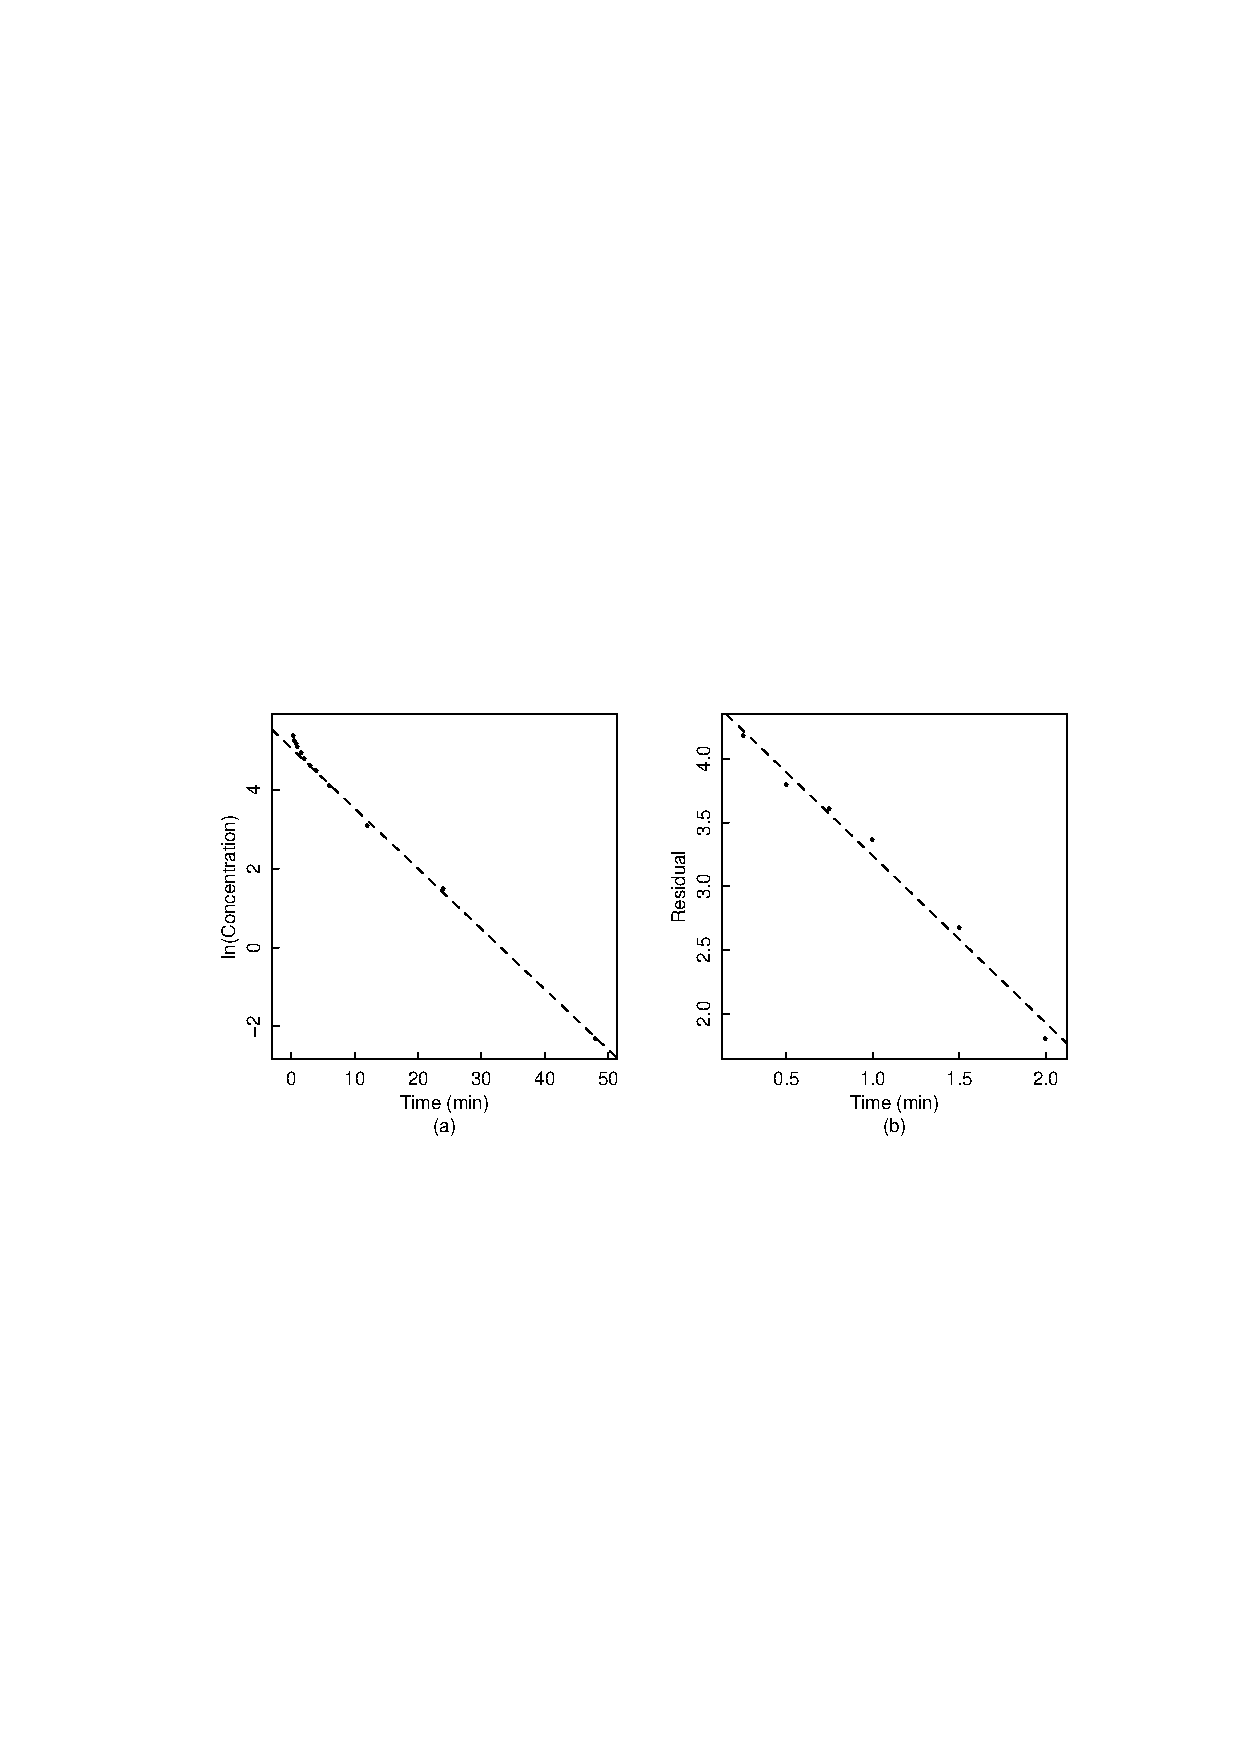
\includegraphics{3SULFstart}}%,width=\textwidth}}
  \caption[Sulfisoxazole curve peeling]{\label{fig:SULFstart}
    Curve peeling using the Sulfisoxazole data.
    In part $a$ we show the data, plotted on a log scale, together with a
    straight line fit (dashed line) to the last six points.
    In part $b$ we show, on a log scale, the residuals for the first six
    data points from the straight line fit in part $a$.
    The dashed line is the fitted line through these (log) residuals.}
\end{figure}
in Figure~\ref{fig:SULFstart}$a$ reveals monotonic decay with straight
line behavior for large $x$, which suggests a model of the form
\begin{displaymath}
  f(x,\btheta)=\theta_1 e^{-\theta_2 x}+\theta_3e^{-\theta_4 x}
\end{displaymath}
with all positive parameters.
Fitting a straight line to the last six (log) data values gives an
intercept of 5.05 and a slope of $-0.153$, so that the
starting values are $\theta_3^{0}= e^{{5.05}}=156$ and
$\theta_4^0 = 0.153$.
Calculating the residuals
\begin{displaymath}
  \tilde y_n = y_n - 156  e^{ - 0.153  x_n }
\end{displaymath}
and plotting $\ln  \tilde y $ versus $x$
for the first six data values, as in Figure~\ref{fig:SULFstart}$b$,
again reveals straight line behavior.
Fitting a straight line to these (log) residuals gives an
intercept of 4.55 and a slope of $-1.31$, so that the
starting values are $\theta_1^0=e^{4.55}=95$ and
$\theta_2 = 1.31$.
\end{example}

\subsection{Reducing Dimensions}
\index{starting values!reducing dimensions}

Peeling is an example of the general technique of reducing dimensions
in order to obtain starting values.  In this technique one estimates
parameters successively, each estimated parameter making it easier to
estimate the remaining ones.  As another example of reducing parameter
dimensions, consider the model
$f = \theta_1 + \theta_2 e^{ - \theta_3 x }$,
where $\theta_{3}$ is positive.  Then the
limiting value of the response when $x\to\infty$ is $\theta_{1}$ and
the value at $x=0$ is $\theta_1+\theta_{2}$.  Depending on
whether the data is increasing or decreasing, we can use
$y_{\mbox{\rm max}}$ or $y_{\mbox{\rm min}}$ to get the starting value
$\theta_1^0$, and then use the difference
$ y ( 0 ) - \theta_1^0 $ to get
$\theta_2^0$.
We perform a linear regression (without a constant term) of
$\ln [ ( y - \theta_1^0 ) / \theta_2^0 ]$ on $x$
to obtain $\theta_3^0$.  Alternatively, once
$\theta_1^{0}$ and $\theta_2^{0}$ are determined, we could
substitute these values into the function and evaluate
$(1/x) \ln [ ( y - \theta_1^0 )/ \theta_2^0 ]$
at selected values of $x$ to obtain $\theta_3^0$.

Sometimes we can reduce the dimensionality of the model and
indirectly reduce the number of parameters.
For example, with the model
$f ( \bx , \btheta )=
\exp [ - \theta_1 x_1 \exp ( - \theta_2 / x_2 )]$,
if there are some very large values of $x_{2}$, then the model
is approximately
$f ( x_1 , \btheta ) = e^{ - \theta_1 x_1 }$, so it is
easy to obtain a starting estimate for $\theta_{1}$ by taking
logarithms of the responses at large $x_{2}$.
Similarly the model
$f ( \bx , \btheta ) = \theta_1 \theta_2 x_1 /
( 1 + \theta_2 x_1 + \theta_3 x_2 )$ reduces
to a Michaelis--Menten type when $x_{2}$ is small, so it is easy
to obtain starting values.
\subsection{Conditional Linearity}
\index{starting values!conditionally linear model}

In many model functions, several of the parameters are conditionally linear
(see Section 2.1) and linear regression can be used to get
starting values for these parameters conditional on the nonlinear
parameters.
Alternatively, special algorithms
which exploit the conditional linearity, described in Section 3.5.5,
can be used.
These algorithms only require starting estimates for the
nonlinear parameters.
As an example of conditional linearity, in
      \begin{displaymath}
        f ( x ,  \btheta ) = \theta_1 + \theta_2 e^{ - \theta_3 x }
      \end{displaymath}
both $\theta_{1}$ and $\theta_{2}$ are conditionally linear,
so it is possible to use linear least squares to estimate
$\theta_1^{0}$ and $\theta_2^{0}$ once an estimate for
$\theta_3^{0}$ has been obtained.
A detailed example involving conditionally linear parameters
\index{parameter!conditionally linear}
is given in Section 3.6.

\section{Parameter Transformations}

As will be shown in Chapters 6 and 7, transforming the parameters in a
nonlinear regression model can produce a much better linear
approximation.  This has the beneficial effects of making approximate
inference regions better and speeding convergence to the least squares
value.  Parameter transformations can also be used to enforce
constraints on the values of the parameters.

Note that transformations of parameters are very different from
transformations of the responses.  Transformations of the response
distort the response space and create a new expectation surface,
thereby affecting the disturbances and the validity of the assumptions
on the disturbances.  In contrast, transformations of the parameters
merely relabel points in the parameter space and on the existing
expectation surface.  Consequently they do not affect the assumptions
about the deterministic or the stochastic parts of the model, although
they do affect the validity of the linear approximation and inferences
based on it.

The use of parameter transformations to improve validity of the linear
approximation is discussed in Chapter 7; here we focus on
transformations to impose constraints on parameters and to improve
convergence.

\subsection{Constrained Parameters}
\index{practical considerations!constraint on parameter}
\index{parameter!constraint}
\index{constraint!on parameter}

The parameters in
most nonlinear models are restricted to regions which make sense
scientifically.
For example, in the Michaelis--Menten model
and in the isomerization model, all the parameters must be
positive, and
in exponential models, the parameters in the exponent
usually must be positive.

It is often possible to ignore the restrictions when fitting
the model and simply examine the converged parameter
estimates to see if they satisfy the constraints.
If the model fits the data well, the parameter estimates should
be in a meaningful range.
Sometimes, though, it may be dangerous to allow the
parameter estimates to go into proscribed regions
during the iterations because the parameter values
may begin to oscillate wildly or
cause numerical overflows.
In these situations, one should impose the constraints throughout the
estimation process.

General techniques for optimizing functions whose parameters are
constrained, called \emph{nonlinear programming}, are beyond the
scope of this book.
See, for example, \citeasnoun{gill:murr:wrig:1981} or
\citeasnoun{bard:1974} for details.
%\glossary{ Gill, P.E.}
%\glossary{ Murray, W.}
%\glossary{ Wright, M.H.}
%\glossary{ Bard, Y.}
Fortunately, the types of constraints that are applied to the parameters of a
nonlinear regression model are usually simple enough to be
handled by parameter transformations.
For example, if $\theta_p $ must be positive, we
reparametrize to $ \phi_p = \ln\theta_p $,
so throughout the iterations
the value of $\theta_p = e^{ \phi_p }$ remains positive.

An \emph{interval} constraint on a parameter, say
\index{constraint!interval}
  \begin{displaymath}
    a  \le  \theta  \le  b
  \end{displaymath}
can be enforced by
a logistic transformation of the form
  \begin{displaymath}
    \theta = a + \frac{b-a}{1 + e^{ - \phi }}
  \end{displaymath}
while an \emph{order} constraint
\index{constraint!order}
on parameters $\theta_j ,\ldots, \theta_{k}$, say
  \begin{displaymath}
    a  \le  \theta_j  \le  \theta_{j+1}  \le  \cdots  \le  \theta_k  \le  b
  \end{displaymath}
can be enforced by a transformation given in \citeasnoun{jupp:1978}.
%\glossary{ Jupp, D.L.B.}

The order constraint can be used to ensure a unique optimum in a model with
exchangeable parameters.
\index{parameter!exchangeable}
As an example of such a model, consider the double exponential model
  \begin{displaymath}
    f ( x , \btheta ) = \theta_1 e^{ - \theta_2  x} +
\theta_3 e^{ - \theta_4  x } 
0 \le \theta_2 ,  \theta_4
  \end{displaymath}
where the pairs of parameters $ ( \theta_1 , \theta_2 )$
and $( \theta_3 , \theta_4 )$ are
\emph{exchangeable}---that is, exchanging the parameter pair
$(\theta_1,\theta_2)$ with the pair $(\theta_3,\theta_4)$ will not 
alter the values of the expected responses.
Exchangeable parameters can create nasty optimization
problems because the linear approximation cannot account for that
kind of symmetry.

In this example, we remove the exchangeability by requiring
  \begin{displaymath}
    0  \le  \theta_2  \le  \theta_4
  \end{displaymath}
and enforce this with the transformation
  \begin{displaymath}
    \theta_2 =e^{ \phi_2 }
  \end{displaymath}
  \begin{displaymath}
    \theta_4 =e^{ \phi_2 }( 1 + e^{ \phi_4 } )
  \end{displaymath}
Since $\theta_{1}$ and $\theta_{3}$ are
conditionally linear parameters, their optimal values are
uniquely determined when $\theta_{2}$ and $\theta_{4}$ are
distinct.
Thus we only need to keep $\theta_{2}$ and $\theta_{4}$ ordered
to eliminate the exchangeability.
\subsection{Facilitating Convergence}
\index{practical considerations!improving convergence}
\index{parameter transformation!to improve convergence}

Parameter transformations can facilitate convergence because they
prevent the parameters from venturing into proscribed regions.
Transformations can also improve convergence by making the
parameter lines behave more uniformly on the expectation surface
so that the Gauss increment is more accurate.
Joint variable--parameter
transformations can also be used to
improve the estimation situation by improving conditioning of
the derivative matrix $\bV$.
\index{derivative matrix!conditioning}
Frequently this is done
by \emph{centering} or \emph{scaling} the data.
\index{parameter transformation!centering and scaling}
\index{improving convergence!centering and scaling}
For example, the simple model
$f ( x , \btheta ) = \theta_1 e^{ - \theta_2  x }$ has derivatives
\begin{displaymath}
  \frac{\partial f}{\partial \theta_1}=e^{-\theta_2 x}
\end{displaymath}
\begin{displaymath}
  \frac{\partial f}{\partial\theta_2}=-x\theta_1e^{-\theta_2 x}
\end{displaymath}
and the derivative vectors tend to be collinear when the values
\index{practical considerations!collinearity}
\index{collinearity}
of $x$ are all positive.
Rewriting the model as
\begin{displaymath}
  f(x,\btheta)=\theta_1 e^{-\theta_2(x-x_0+x_0)}
\end{displaymath}
and reparametrizing with
\begin{displaymath}
  \phi_1=\theta_1e^{-\theta_2 x_0}
\end{displaymath}
\begin{displaymath}
  \phi_2=\theta_2
\end{displaymath}
gives $f(x,\bphi)=\phi_1e^{-\phi_2(x-x_0)}$,
and now the derivatives with respect to $\bphi$ will be more
nearly orthogonal.
A useful choice is $x_0=\bar{x}$.

\emph{Scaling} the variables and the parameters can
also improve conditioning by making the derivative matrix have
column vectors which are more nearly equal in length.

Other transformations can be useful, depending on the context of
the problem.
For example, in chemical kinetics it is often useful to revise
the model so that reciprocal absolute temperature is used rather
than temperature $T$.
Combining this with centering would then modify a term involving
temperature to the form
$1/T-1/T_{0}$.

The effect of parameter transformations on parameter effects
nonlinearities and the adequacy of linear approximation inference
regions is discussed in Chapter 7.

\section{Other Iterative Techniques}

The Gauss--Newton iterative algorithm for nonlinear least squares,
described in Section 2.2.1, is a simple, useful method for
finding $\hat{\btheta}$.
Some modifications to this method, as well as alternative methods,
have been suggested---primarily to deal with ill-conditioning of
the derivative matrix $\bV$ and to avoid having to
code and specify the derivatives.
\subsection{A Newton--Raphson Method}

The Gauss--Newton method for estimating nonlinear parameters can be
\index{Gauss-Newton!iteration method}
considered as a special case of the more general Newton--Raphson method
\index{Newton-Raphson!iteration method}
\cite{bard:1974} which uses a local quadratic approximation to the
%\glossary{ Bard, Y.}
objective function.
Near $\btheta^{0}$, we approximate
\begin{displaymath}
  S ( \btheta ) \approx S ( \btheta^0 )
  + {\bomega} \trans ( \btheta - \btheta^0 )
  + ( \btheta - \btheta^0 )\trans\frac{\bOMEGA}{2}(\btheta-\btheta^0)
\end{displaymath}
where
\begin{displaymath}
  \bomega  = \frac{\partial S}{\partial \btheta}
\end{displaymath}
is the \emph{gradient}
\index{gradient!of sum of squares function}
of $S ( \btheta )$ evaluated at $\btheta^{0}$
and
\begin{displaymath}
  \bOMEGA=\frac{\partial^2 S}{\partial\btheta\partial\btheta\trans}
\end{displaymath}
is the \emph{Hessian}
\index{Hessian!of sum of squares function}
of $S(\btheta)$ evaluated at $\btheta^{0}$.
The approximating sum of squares function will have
a stationary point when its gradient is zero---that is, when
\begin{displaymath}
  \bomega+\bOMEGA(\btheta-\btheta^0)=\bm0 
\end{displaymath}
and this stationary point will be a minimum if $\bOMEGA$ is positive
definite (all its eigenvalues positive).
If $\bOMEGA$ is positive definite, the Newton--Raphson step is
\begin{displaymath}
  \bdelta^0=-\bOMEGA^{-1}\bomega .
\end{displaymath}

For the function
\begin{displaymath}
  S(\btheta)=(\by-\boeta)\trans(\by-\boeta)
\end{displaymath}
the gradient is
\begin{displaymath}
  \bomega=-2\bV\trans(\by-\boeta)
\end{displaymath}
and the Hessian is
\begin{displaymath}
  \bOMEGA=2\bV\trans\bV-2\frac{\partial\bV\trans}{\partial\btheta\trans}(\by-\boeta)
\end{displaymath}
where $\bV$ is the derivative matrix.
The Gauss--Newton increment is therefore equivalent to the
Newton--Raphson increment with the second derivative term
${\partial\bV\trans}/{\partial\btheta\trans}$ set to zero.

\citeasnoun{denn:gay:wels:1981} describe a nonlinear least squares
%\glossary{ Dennis, J.E.Jr.}
%\glossary{ Gay, D.M.}
%\glossary{ Welsch, R.E.}
routine which develops a quasi-Newton approximation \cite{denn:schn:1983}
to the second term in the Hessian.
%\glossary{ Dennis, J.E.Jr.}
%\glossary{ Schnabel, R.B.}
This extends the Gauss--Newton algorithm and makes it closer to the
Newton--Raphson algorithm,
which has the advantage that the approximating Hessian should be closer
to the actual Hessian than the single term $\bV \trans \bV$ used in
the Gauss--Newton algorithm.
However, the term $\bV \trans \bV$ is necessarily positive definite
(or at least positive semidefinite),
since the eigenvalues of $\bV \trans \bV$ are the squares of the singular
values of $\bV$.
Adding another term on to this to form an approximating
Hessian can destroy the positive definiteness, in which case the
Newton--Raphson algorithm must be modified to restore
positive definiteness in the Hessian.
\subsection{The Levenberg--Marquardt Compromise}
\index{practical considerations!Levenberg--Marquardt compromise}
\index{Levenberg--Marquardt compromise}

A condition that can cause erratic behavior of Gauss--Newton
iterations is singularity of the derivative
matrix $\bV$ caused by collinearity of the columns.
\index{practical considerations!collinearity}
\index{collinearity}
When $\bV$ is nearly singular,
$\bdelta$ can be very large, causing the parameters to go into
undesirable regions of the parameter space.

One solution to the problem of near-singularity is to perform the
calculations for the increment in a numerically stable way, which is why
we recommend using the $QR$ decomposition rather than
\index{practical considerations!QR decomposition}
the normal equations.
We also recommend using double precision or extended
precision arithmetic for the calculations, where feasible, and
using joint variable--parameter transformations as discussed in
Section 3.4.

Another general method for dealing with near-singularity is
to modify the Gauss--Newton increment to
  \begin{displaymath}\label{eqn:levenberg}
    \bdelta (k)=( \bV \trans \bV+k \bI )^{-1}
    \bV \trans ( \by - \boeta )
  \end{displaymath}
as suggested in \citeasnoun{leve:1944}, or to
%\glossary{ Levenberg, K.}
  \begin{displaymath}\label{eqn:marquardt}
    \bdelta (k) = ( \bV \trans \bV + k \bD )^{-1}
    \bV \trans ( \by - \boeta )
  \end{displaymath}
as suggested in \citeasnoun{marq:1963}, where $k$ is a conditioning factor
%\glossary{ Marquardt, D.W.}
and $\bD$ is a diagonal matrix with entries equal to the
diagonal elements of $\bV \trans \bV$.
This is called the \emph{Levenberg--Marquardt compromise}
because
\index{practical considerations!Levenberg--Marquardt compromise}
\index{Levenberg--Marquardt compromise}
the direction of $\bdelta (k)$ is intermediate between the direction
of the Gauss--Newton increment ($k\to 0$)
\index{Gauss-Newton increment}
and the direction of \emph{steepest descent}
\index{steepest descent}
$\bV\trans(\by-\boeta)/\norm\bV\trans(\by-\boeta)\norm$ ($k\to\infty$).

Note that Levenberg recommends inflating the diagonal of
$\bV \trans \bV$ by an additive factor, while Marquardt recommends
inflating the diagonal by a multiplicative factor $1 + k$.
Marquardt's method produces an increment which is invariant under
scaling transformations of the parameters, so that
if the scale for one component of the parameter
vector is doubled, the increment calculated, and the
corresponding component of the increment halved, the result
will be the same as calculating the increment in the original
scale.
In Levenberg's method, this is not true.
\citeasnoun{box:kane:1984} showed, however, that if one
%\glossary{ Box, G.E.P.}
%\glossary{ Kanemasu, H.}
requires invariance of the increment under linear
transformations of the parameter space, the resulting increment is the
Gauss--Newton increment with a step factor.

The Levenberg--Marquardt compromise is more difficult to implement
than the Gauss--Newton algorithm, since one must decide
how to manipulate both the conditioning factor $k$ and the step
factor $\lambda$; nevertheless
it is implemented in many nonlinear least squares programs.
Although we presented the increment in terms of the inverse of an
augmented $\bV \trans \bV$ matrix, the actual calculations for the
increment should be done using a $QR$ decomposition of $\bV$ and
applying updates from a diagonal matrix using the Givens
rotations \cite{golu:pere:1973,dong:bunc:mole:stew:1979}, (Chapter 10),
%\glossary{ Golub, G.H.}
%\glossary{ Pereyra, V.}
%\glossary{ Dongarra, J.J.}
%\glossary{ Bunch, J.R.}
%\glossary{ Moler, C.B.}
%\glossary{Stewart, G.W.}
since the Levenberg increment (\ref{eqn:levenberg}) is the least squares
solution to the system with derivative matrix
\begin{displaymath}
  \begin{bmatrix}\bV\\\sqrt k\bI \end{bmatrix}
\end{displaymath}
and response vector
\begin{displaymath}
  \begin{bmatrix}\by-\boeta\\\bm0\end{bmatrix}
\end{displaymath}
For the Marquardt increment (\ref{eqn:marquardt}), the derivative matrix
is changed to
\begin{displaymath}
  \begin{bmatrix}\bV\\\sqrt k\bD^{1/2}\end{bmatrix}
\end{displaymath}
\subsection{Numerical Derivatives}
\index{practical considerations!numerical derivatives}

We have assumed that implementations of the algorithms we have
described use analytic derivatives with respect to the parameters.
Obtaining these derivatives and coding them
is usually the most tedious and error-prone stage in a
nonlinear analysis.

As a general rule we recommend using analytic derivatives for
accuracy, although it is convenient to use programs which use
numerical derivatives from finite differences.
Such convenience is not obtained without cost, however, because
numerical derivatives can be inaccurate and they usually increase the
computing time necessary to obtain convergence.
Furthermore, if second derivatives are required to investigate the
effect of nonlinearity on inferences, the numerical second derivatives
evaluated from numerical first derivatives can be very
inaccurate.
Other problems with numerical derivatives involve the choice of
step size to determine the finite differences, and whether to use
central or forward differences.

With forward differences, for the $p$th
parameter we evaluate the model function
using the current values of all the
parameters except for the $p$th, which is incremented
to $\theta_p ( 1 + \epsilon )$.
Dividing the differences between the function values
by the fractional amount $\epsilon \theta_{p}$
gives an approximate derivative.
This requires $1 + P$ evaluations of the expected response
vector at each iteration.
Using central differences would require evaluation of the model
function at
$\theta_p ( 1 \pm \epsilon )$ in addition to the central
value, so the total number of evaluations would be
$1 + 2 P$.
%{.dennis schnabel 1983.}
Dennis and Schnabel (1983) recommend setting $\epsilon$ equal to the
%\glossary{ Dennis, J.E.Jr.}
%\glossary{ Schnabel, R.B.}
square root of the relative machine precision (that is, the square
root of the smallest number which, when added to 1.0 in
the floating point arithmetic of the computer, produces a number
greater than 1.0).
\subsection{Derivative-Free Methods}
\index{practical considerations!derivative-free methods}

There are derivative-free methods which do not simply use
numerical approximations to derivatives.
\citeasnoun{rals:jenn:1978} introduced one such routine, DUD
%\glossary{ Ralston, M.L.}
%\glossary{ Jennrich, R.I.}
\index{DUD}
(Doesn't Use Derivatives), which is
based on using a secant plane approximation to the
expectation surface rather than a tangent plane approximation.

To use DUD, one must provide starting values $\btheta^{0}$.
The program then automatically produces a further set of $P$ parameter
vectors by displacing each parameter in turn by 10\%.
These parameter vectors are then used to calculate expectation
vectors $\boeta_{1}$, $\boeta_2 ,\ldots,$ giving a
secant plane which matches the expectation surface at
$P + 1$ points.
A set of linear coordinates is generated on the secant plane, and
the projection of $\by$ onto the secant plane is made and
mapped into the parameter plane.
This information is used to calculate a new $\btheta$ vector,
say $\btheta '$, for which $\boeta ( \btheta ' )$ is
closer to $\by$ than any of the other parameter vectors.
The parameter vector $\btheta$ corresponding to the
$\boeta$ which is farthest from $\by$ is then replaced by
$\btheta '$, and the process continued until convergence is
achieved.
\label{rum:dud}
\begin{example}

DUD can be illustrated very effectively using
a two-observation example such as in Example Rumford 2.
To simplify arithmetic and to provide a better scale for the
figure, we provide the necessary two $( = P + 1 )$ starting
values rather than using the automatic 10\% displacement.
The two starting values are chosen to be $\theta^1=0.02$
and $\theta^2=0.10$.
Figure~\ref{fig:RUM2dud} shows the expectation surface
  \begin{figure}
    \vspace{3in}
    \centerline{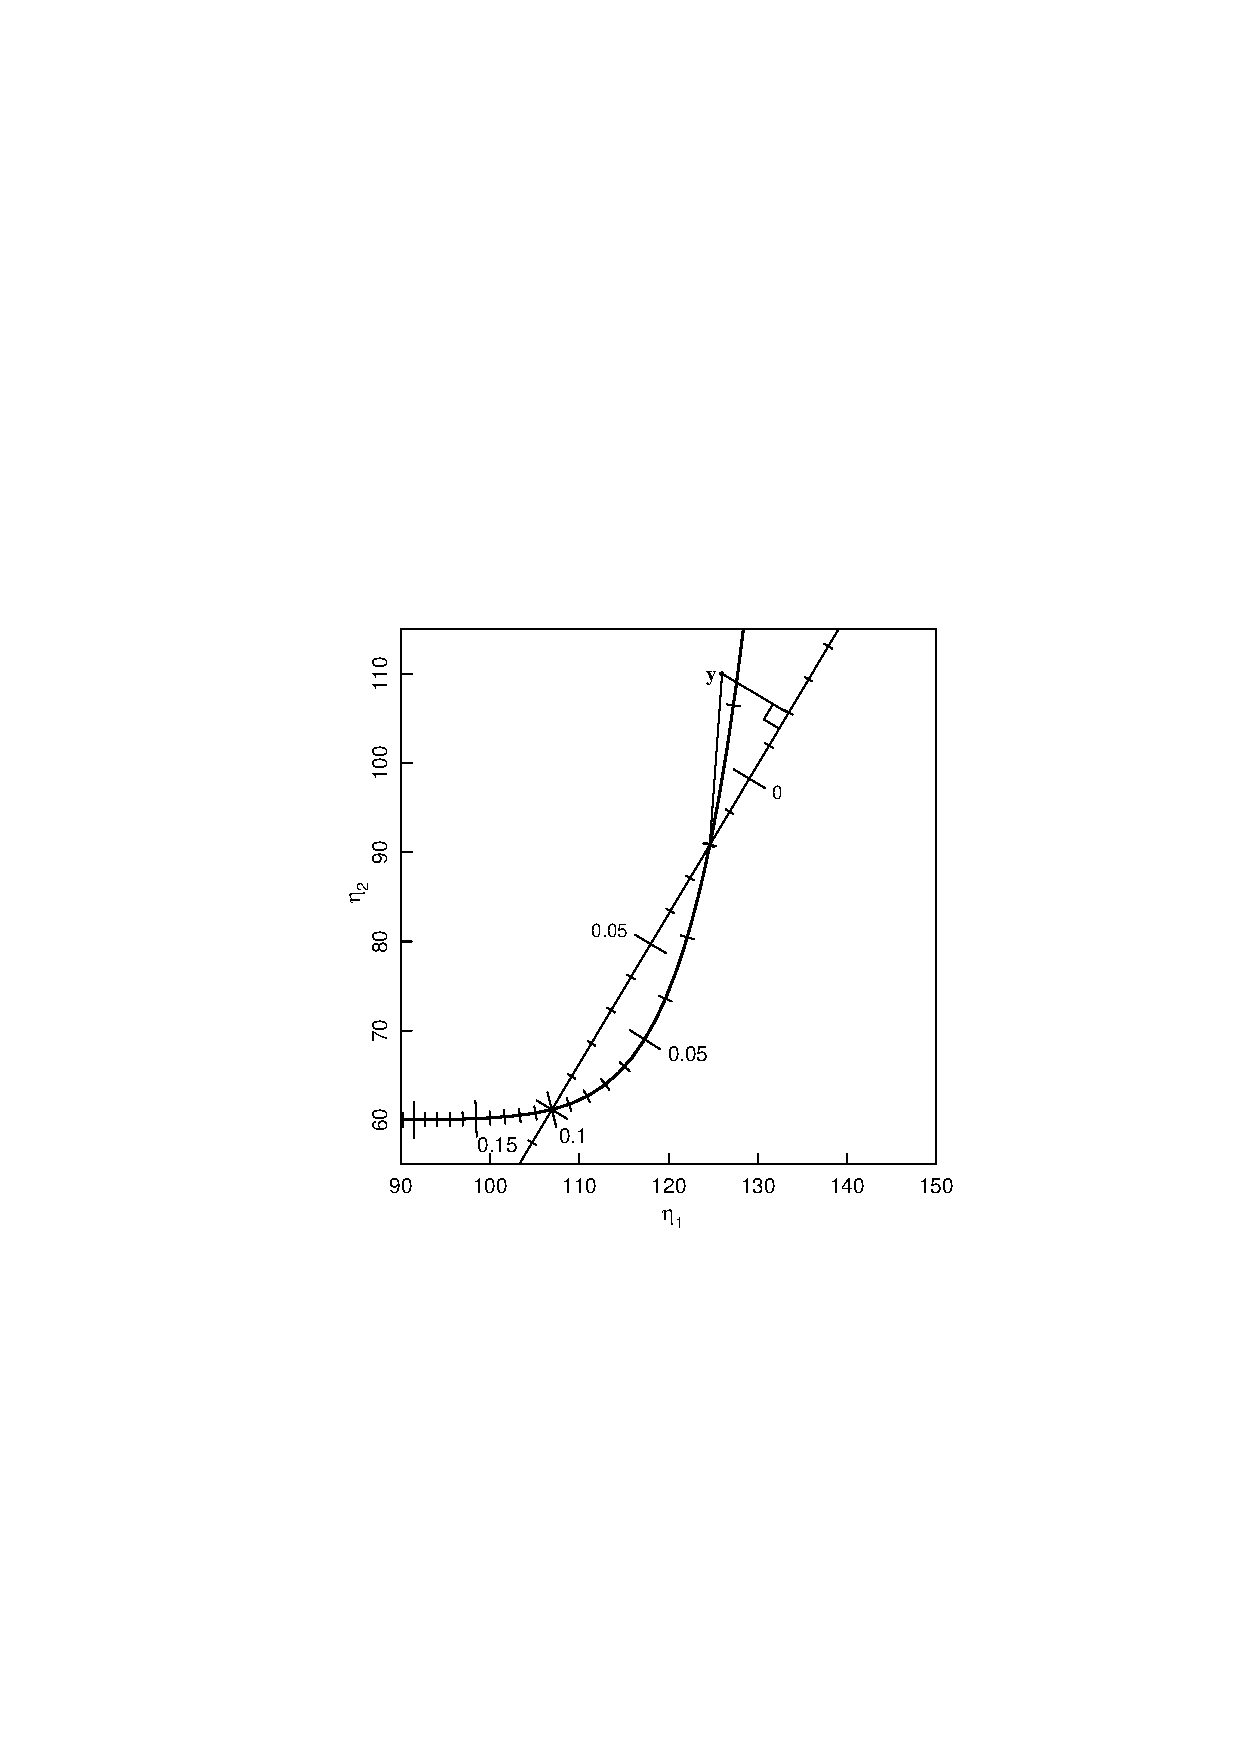
\includegraphics{3RUM2dud}}%,height=3in}}
    \caption[Geometric representation of DUD]{
    A geometric interpretation of the calculation of the DUD
    increment using the 2-case Rumford data.
    A portion of the expectation surface (heavy solid line) is shown in
    the response space together with the observed response $\by$.
    Also shown is the projection of $\by-\boeta ( 0.02 )$ onto the
    secant plane joining $\boeta ( 0.02 )$ and $\boeta ( 0.10 )$
    (solid line).
    The tick marks indicate true positions on the expectation surface and
    linear approximation positions on the secant plane.
    }
    \label{fig:RUM2dud}
  \end{figure}
$\boeta ( \theta )$ together with the secant line
$\bl$ through the points
$\boeta ( \theta^1 )$ and $\boeta ( \theta^2 )$.
We now introduce a linear scale parameter $\alpha$ on $\theta$ such
that $\theta =\theta^1+T\alpha$, where
$T = (\theta^2-\theta^1)$ and so $\alpha=0$ at
$\theta^{1}$ and $\alpha = 1$ at $\theta^{2}$.
We also impose a linear scale on $\bl$ such that
$\bl ( \alpha )=\boeta ( \theta^1 )+\bH \alpha$,
where $\bH=\boeta ( \theta^2 )-\boeta ( \theta^1 )$.
The linear coordinate system is also shown in Figure~\ref{fig:RUM2dud}.

For this example, $T=\theta^2-\theta^1=0.08$,
$\theta=\theta^1+T\alpha$, so 
\begin{displaymath}
  \alpha =\frac{\theta-\theta^1}{T}
\end{displaymath}
\begin{eqnarray*}
  \bH&=&
  \begin{bmatrix}
    60+70e^{{-4(0.1)}}\\
    60+70e^{ -41(0.1)}
  \end{bmatrix} -
  \begin{bmatrix}
    60+70e^{-4(0.02)}\\
    60+70e^{-41(0.02)}
  \end{bmatrix}\\
  &=&\begin{bmatrix}106.92 \\ 61.16\end{bmatrix} -
  \begin{bmatrix}124.62 \\ 90.83\end{bmatrix}\\
  &=&\begin{bmatrix}-17.70 \\ -29.67\end{bmatrix}
\end{eqnarray*}
and
\begin{eqnarray*}
  \bl&=&\boeta ( \theta^1 )+\bH \alpha\\
  &=&\begin{bmatrix}124.62 \\ 90.83\end{bmatrix} +
  \begin{bmatrix}-17.70 \\ -29.67\end{bmatrix}
  \alpha
\end{eqnarray*}
We now use linear least squares to project the residual vector
\begin{eqnarray*}
  \by-\bl (0)&=&\begin{bmatrix}126 \\ 110\end{bmatrix} -
  \begin{bmatrix}124.62 \\ 90.83\end{bmatrix}\\
  &=&\begin{bmatrix}1.38 \\ 19.17\end{bmatrix}
\end{eqnarray*}
onto $\bl$ to obtain
\begin{displaymath}
  \hat{\alpha}=( \bH \trans \bH )^{-1}
  \bH \trans ( \by - \bl ( 0 ) )
\end{displaymath}
For this example
\begin{displaymath}
  \hat{\alpha}=-0.49
\end{displaymath}
so new value of $\theta$ is
\begin{eqnarray*}
  \theta_{\mbox{\rm new}}&=&0.02+T ( - 0.49 )\\
  &=&0.02 + 0.08 ( -0.49 )\\
  &=&-0.019
\end{eqnarray*}
Evaluating the sum of squares at this point reveals that this new
point is farther from $\by$ than either of the two starting
points, and so a step factor $\lambda$ is introduced to
\index{step factor}
search along the increment vector to determine a better point.
Incorporating $\lambda$ as
  \begin{displaymath}
    \theta_{\mbox{\rm trial}} = \theta_{\mbox{\rm new}} \lambda +
    \theta_{\mbox{\rm old}} ( 1 - \lambda )
  \end{displaymath}
gives, for this example,
  \begin{displaymath}
    \theta_{\mbox{\rm trial}} = (- 0.019) \lambda + 0.02 ( 1 - \lambda )
  \end{displaymath}
and the minimum occurs at $\lambda = 0.5$ with
$\theta_{\mbox{\rm trial}} = 0.0005$.
The point $\theta^2=0.10$ is then replaced by $\theta^3=0.0005$
and the process is repeated using the pair
$( \theta^1 , \theta^3 )$.
\end{example}

In the general case of $P$ parameters, at the $i$th iteration
we use the values of $\boeta ( \btheta )$ at
$\btheta_1^i , \btheta_2^i ,\dots, \btheta_{P+1}^{i}$
to determine the secant plane
as the $P$-dimensional plane which passes through
$\boeta ( \btheta_p^i )$, $p = 1 ,\ldots, P+1$.
For convenience, we assume that $\btheta_{P+1}^{i}$
corresponds to the point closest to $\by$;
we then determine the $P\times P$
matrix $\bT$ by setting its $p$th column
equal to $\btheta_p^i - \btheta_{P+1}^{i}$,
and the $N\times P$
matrix $\bH$ by setting its $p$th column equal to
$\boeta ( \btheta_p^i ) -
\boeta ( \btheta_{P+1}^i )$.
Then, formally,
\begin{eqnarray*}
  \hat{\balpha}&=&( \bH \trans \bH )^{-1} \bH \trans
  [ \by - \boeta ( \btheta_{P+1}^i ) ]\\
  \btheta_{\mbox{\rm new}}&=&\btheta_{P+1}^i + \bT \hat{\balpha}
\end{eqnarray*}
and
\begin{displaymath}
  \btheta_{\mbox{\rm trial}} = \btheta_{\mbox{\rm new}}\lambda+
  \btheta_{P+1}^i (1-\lambda)
\end{displaymath}
Note that
\citeasnoun{rals:jenn:1978} allow the step factor to be negative,
%\glossary{ Ralston, M.L.}
%\glossary{ Jennrich, R.I.}
\index{step factor}
by choosing $\lambda$ from a sequence of values
$1,1/2,-1/4,1/8,-1/16,\cdots$.
At convergence the linear approximation parameter covariance
\index{parameter!approximate covariance matrix}
matrix is given by $s^2 \bT ( \bH \trans \bH )^{-1} \bT \trans$,
where $s^{2}$ is the usual variance estimate.
Note that the matrix $\bT$ may be
ill conditioned by the time convergence is achieved and so the linear
approximation standard errors and correlations may not be reliable.
\subsection{Removing Conditionally Linear Parameters}

One way of simplifying a nonlinear regression problem is to
eliminate conditionally linear parameters.
\index{conditionally linear!parameter}
\index{parameter!conditionally linear}
\index{practical considerations!conditionally linear parameter}
As mentioned in Sections 2.1 and 3.3.5,
the optimal values of the conditionally linear
parameters, for fixed values of the nonlinear parameters, can be
determined by linear least squares.
If we partition the parameter vector $\btheta$ into the conditionally
linear parameters $\bbeta$ of dimension $P_{1}$
and the nonlinear parameters $\bphi$ of dimension $P_{2}$ with
$P = P_1 + P_{2}$,
the expected responses can be written
\begin{displaymath}
  \boeta ( \bbeta , \bphi ) = \bA ( \bphi ) \bbeta
\end{displaymath}
where the $N\times P_{1}$ matrix $\bA$ depends only on the
nonlinear parameters.
For any value of $\bphi$, the conditional estimate of $\bbeta$ is
\begin{displaymath}
  \hat{\bbeta} ( \bphi ) = \bA^+ ( \bphi )  \by
\end{displaymath}
where $\bA^+ = ( \bA \trans \bA )^{-1} \bA \trans$
is the pseudoinverse of $\bA$.
The associated expected responses are
\begin{displaymath}
  \hat{\boeta}( \bphi ) = \bA ( \bphi ) \bA^+ ( \bphi )  \by
\end{displaymath}
\citeasnoun{golu:pere:1973} formulated a Gauss--Newton algorithm to minimize
%\glossary{ Golub, G.H.}
%\glossary{ Pereyra, V.}
the reduced sum of squares function
\begin{displaymath}
  S_2 ( \bphi ) =
\norm \by - \bA ( \bphi ) \hat{\bbeta}( \bphi ) \norm^2
\end{displaymath}
that depends only on the nonlinear parameters.
In particular, they give the derivative
of $\bA^+ ( \bphi )$ with respect to $\bphi$, which is the key
ingredient in the algorithm.
The expression for this derivative is used in Chapter 4,
where we present a Gauss--Newton algorithm for multiresponse
parameter estimation.

One difficulty with using projection over the conditionally
linear parameters is that additional information about the
parameters must be given by the user.
The user must specify which parameters are conditionally linear
as well as specifying the derivatives of the entries of $\bA$ with
respect to $\bphi$.
This often results in more difficulty than
simply ignoring the conditional linearity.
There are some structured problems, however---such as spline
regression with knot positions allowed to vary, as described in
\citeasnoun{jupp:1978}---where the division between conditionally linear and
%\glossary{ Jupp, D.L.B.}
nonlinear parameters is inherent in the specification of the
problem, so the Golub--Pereyra method can be used to advantage.
These methods are discussed further in \citeasnoun{kauf:1975} and
%\glossary{ Kaufman L.}
\citeasnoun{bate:lind:1986}.
%\glossary{ Bates, D.M.}
%\glossary{ Lindstrom, M.J.}

\section{Obtaining Convergence}
\index{practical considerations!obtaining convergence}
\index{convergence!practical considerations}

Obtaining convergence is sometimes difficult.
If you are having trouble, check the following:
  \begin{itemize}
    \item Is the expectation function correctly specified?
    \item Is the expectation function correctly coded?
    \item Are the derivatives correctly specified?
    \item Are the derivatives correctly coded?
    \item Are the data entered correctly?
    \item Are all the observations reasonable?
    \item Is the response variable correctly identified?
    \item Do the starting values have the correct values?
    \item Do the starting values correspond to the correct parameters?
  \end{itemize}

If the answer to all these questions
is yes, look carefully
at the output from the optimization program.
Most good programs can produce detailed output on each
iteration to help find out what is wrong.
Check to see that the initial sum of squares, $S ( \btheta^0 )$, is
smaller than the sum of squares of the responses.
If not, then the fitted function is worse than no function
and, in spite of your checks, you probably have an incorrect
expectation function, or incorrect data, or incorrect starting
values.
You may even be trying to fit an $x$ variable rather
than the response $y$.

Look at the parameter values.
Do the starting values have the correct magnitudes?
Correct signs?
And are they assigned to the correct parameters?

Next, look at the parameter increments.
Are they all of roughly the same magnitude relative to the
parameters?
Does the increment, when added to the parameter vector, place the
parameter vector in a bad region in the parameter space?
For example, are any necessarily positive parameters driven
negative?
Do any of the parameters become unreasonably large or small?
If so, could there be an error in the derivative functions?
Try using numerical derivatives at a few design points to check
the analytic derivatives.
Would different starting values for some of the parameters help?
Is there a transformation of the parameters which could help?

Sometimes convergence is not achieved because the model has too
many parameters.
Look at the parameter values to see whether any of them are being
driven to extreme values corresponding to a simpler model function.
Also look at combinations of the parameter increments to see, for
example, if pairs of them tend to move together, suggesting
collinearity or possibly overparametrization.
\index{overparametrization}
If there is a suspicion of overparametrization, try simplifying
the expectation function, even temporarily---it may be that a
simpler model will produce better parameter estimates, so that
eventually the full model can be fitted.

Check to see that there are enough data in all regions of
the design space so that valid parameter estimates can be obtained.
For example, when fitting a transition type model in which there
is, say, linear behavior to the left of a point and different
linear behavior to the right
\cite{baco:watt:1971,hink:1969,watt:baco:1974},
%\glossary{ Bacon, D.W.}
%\glossary{ Watts, D.G.}
%\glossary{ Hinkley, D.V.}
it is often the case that there are
lots of data values to define the behavior away from the join
point, but not many near the join point.
In this situation, the parameter which describes the sharpness of
transition will be poorly estimated, and so convergence may be
slow.

When dealing with a comprehensive model which involves combining
data from several experiments, it is generally good practice to
fit each data set with a possibly simpler restricted model, and
gradually extend the model by incorporating more data sets and
parameters.
An example of this is given in \citeasnoun{zieg:1985}.
%\glossary{ Ziegel, E.R.}
Conversely, a large data set which has several reasonably
distinct operating regions can be blocked into small subsets on
that basis, so that a reduced model can be fitted to each subset
and the results used to provide starting estimates for a model
for the full data set, as illustrated below.
\label{lub:converge}
\begin{example}

To illustrate the process of getting starting values and obtaining
convergence for a complicated nonlinear model function, we consider
data on the kinematic viscosity of a lubricant as a function of
temperature ($x_{1}$) and pressure ($x_{2}$).  The data, discussed
in \citeasnoun{lins:1975}, are reproduced in
%\glossary{ Linssen, H.N.}
Appendix A, Section~\ref{atbl:lub}, and plotted in Figure \ref{fig:LUBdata}.
\begin{figure}
  \vspace{3in}
  \centerline{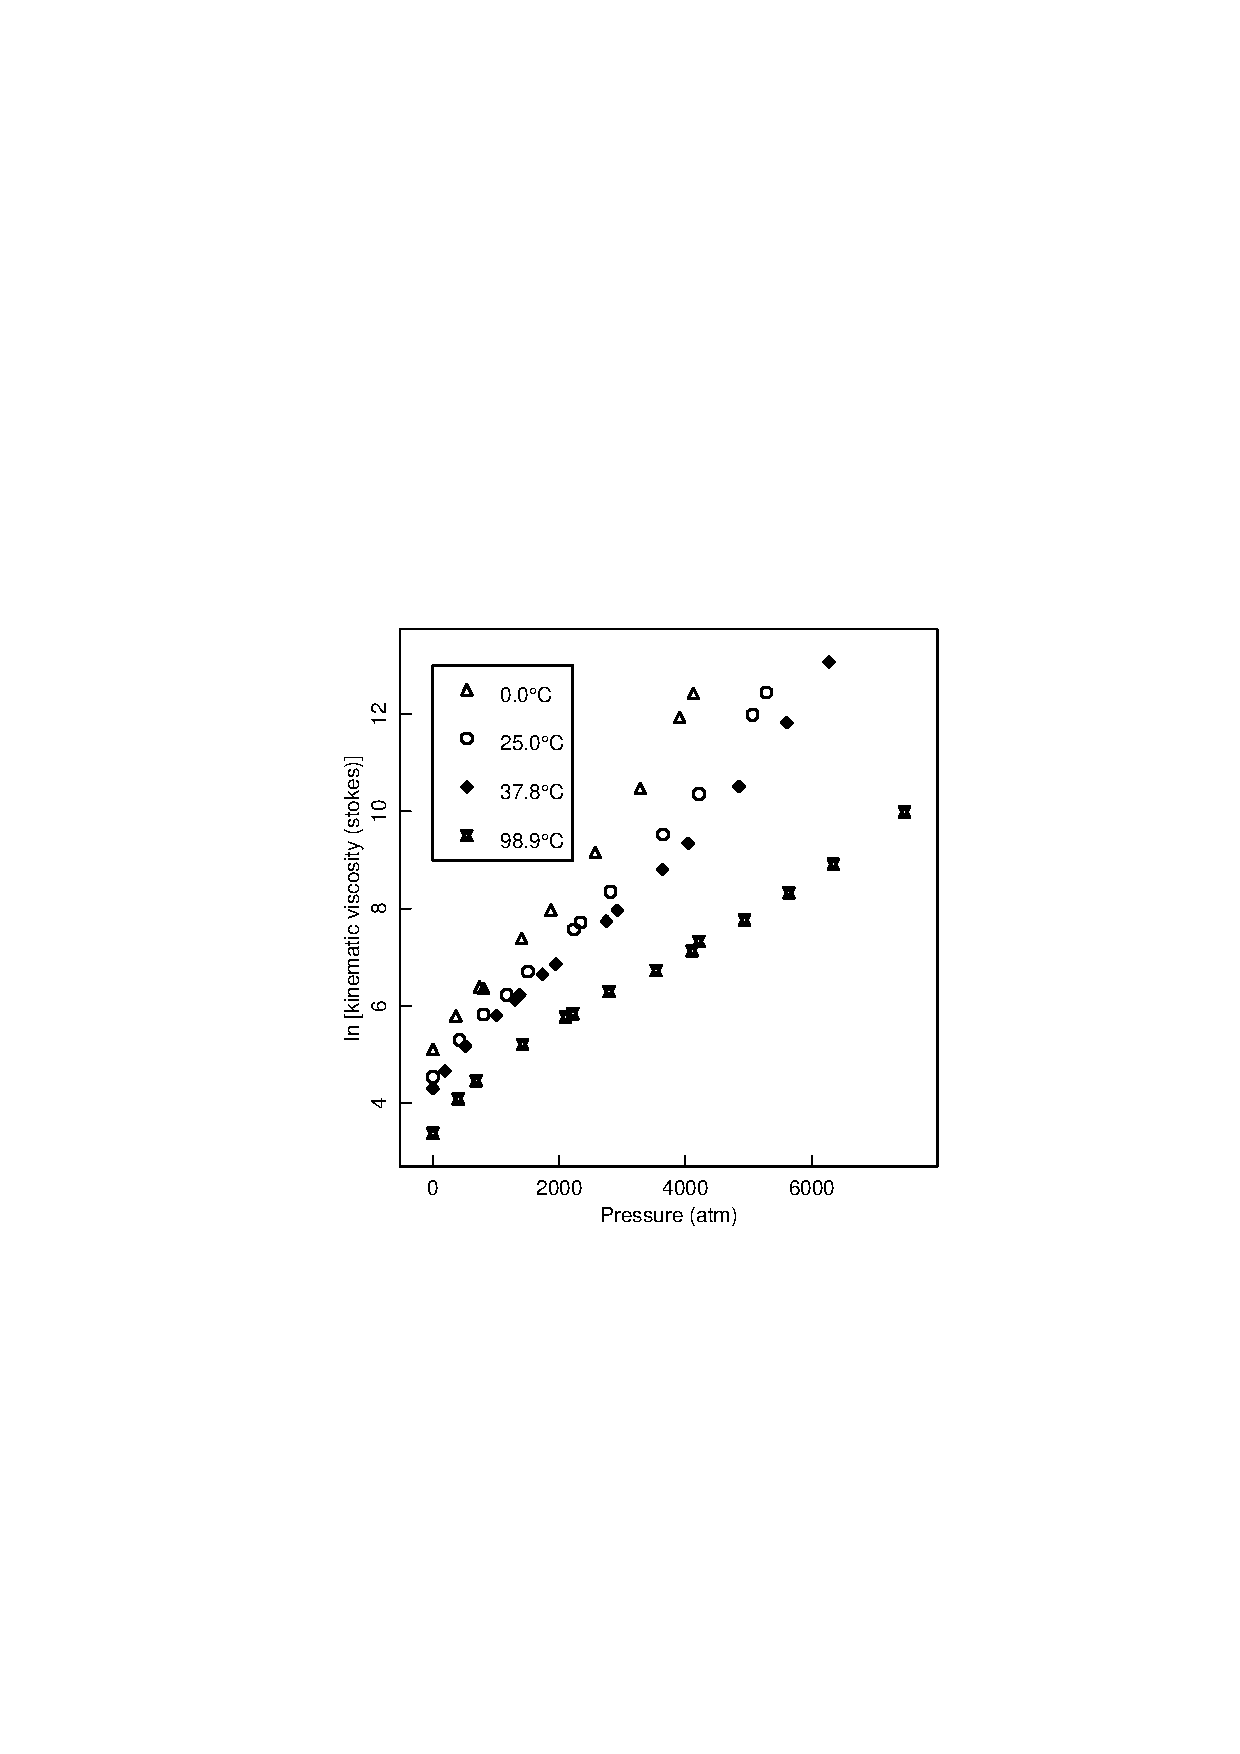
\includegraphics{3LUBdata}}%,height=3in}}
  \caption{
    Plot of the logarithm of the kinematic viscosity of a lubricant versus
    pressure for four different temperatures.
  }\label{fig:LUBdata}
\end{figure}
The model function is
\begin{eqnarray}\label{eqn:lub}
  f (\bx,\btheta)&=&\frac{\theta_1}{\theta_2+x_1}+
  \theta_3 x_2+\theta_4 x_2^2 +
  \theta_5 x_2^3\\
  &&+( \theta_6 + \theta_7 x_2^2 )  x_2 
  \exp \left(\frac{-x_1}{\theta_8+\theta_9 x_2^2}
  \right)\nonumber
\end{eqnarray}

To begin, we note that six of the nine parameters are
conditionally linear, which is most helpful.
Also, to improve conditioning, as discussed in Section 3.4.1, we scale
the pressure data $x_{2}$ by dividing by $1000$ and avoid
confusion by writing $w_2=x_2 / 1000$.

To obtain a starting estimate for $\theta_{2}$, we use the
data for $w_2 = 0.001$ and assume that for this low value of
scaled pressure, the model is a
function of $x_{1}$ only.
Taking reciprocals and using linear least squares as
described in Section 3.3.3 gives $\theta_1^0 = 983$
and $\theta_2^0 = 192$.

Now we exploit the conditional linearity in the model
because we can use linear least squares
to obtain starting estimates for the remaining parameters
once we have reasonable estimates for
$\theta_{8}$ and $\theta_{9}$.
Thus we concentrate on getting estimates for only
these two.
We simplify the situation even more by assuming that
when $w_{2}$ is small,
the model function is essentially linear in $w_{2}$, so that
\begin{displaymath}
  f(\bx,\btheta)\approx\frac{\theta_1}{\theta_2+x_1}+\theta_3w_2+\theta_6w_2e^{-x_1/\theta_8}
\end{displaymath}
That is, we can ignore the terms involving $\theta_{4}$,
$\theta_{5}$, $\theta_{7}$, and $\theta_{9}$.
By examining the plot, we see that the data for each temperature
follow quite straight lines for $w_22$, so we choose
this for the range.
Also, for fixed values of $x_{1}$, the leading term and the
exponential term are constant and we may rearrange the model as
  \begin{eqnarray*}
    y'&=&\theta_3 w_2 + \theta_6 w_2  g\\
    &=&w_2  \beta
  \end{eqnarray*}
where
\begin{displaymath}
  y'=\frac{y-983}{192+x_1}
\end{displaymath}
\begin{displaymath}
g = e^{ - x_1 / \theta_8 }
\end{displaymath}
and
\begin{displaymath}
\beta = \theta_3 + \theta_6 g
\end{displaymath}

Regressing $y'$ on $w_{2}$ for each of the four temperatures
0, 25, 37.8, 98.9 gives $\beta$ values of 1.57, 1.49, 1.39, 1.37.
We now use the $\beta$ values and the relation
$g = e^{ - x_1 / \theta_8 }$
to obtain estimates for $\theta_{3}$ and $\theta_{6}$ by
noting that when $x_1=0$ we have $g=1$,
so $\beta=\theta_3+\theta_{6}$,
and when $x_1\to\infty$ $\beta=\theta_{3}$.
We therefore estimate the sum of the two parameters as 1.57
(the value of $\beta$ at $x_1 = 0$), and
assuming that the lower asymptote has almost been reached at the
highest temperature,
we choose $\theta_{3}$ to be 1.35, which is a bit smaller than 1.37
(the value of $\beta$ at $x_1=98.9$).
The value for $\theta_{6}$ is then estimated as
$1.57 - 1.35 = 0.22$.
Finally, since $\beta=\theta_3 + \theta_6 g$, so
$( \beta-\theta_3 ) / \theta_6 =g$, we regressed
\begin{displaymath}
ln \left(\frac{\beta-1.35}{0.22}\right)
\end{displaymath}
on $x_1 $ to give $\theta_8 = 35.5$.

Using these parameter estimates for
$\theta_{2}$ and $\theta_{8}$,
we performed a nonlinear regression on
the data for small $w_{2}$ values to get more refined
estimates, $\theta_2 = 202$ and $\theta_8 = 35.90$.
We then used these estimates for $\theta_{2}$ and
$\theta_{8}$, and the data for all $w_{2}$ values,
to estimate all the parameters with $\theta_9 = 0$.
The new values were $\theta_2=209$ and $\theta_8=47.55$.
Finally, we used these values plus the starting value
$\theta_9 = 0$ to converge on the full model.
The final parameter estimates were
\begin{displaymath}
\hat{\btheta}=
(1053,206.1,1.464,-0.259,0.0224,0.398,0.09354, 56.97,-0.463)\trans
\end{displaymath}
with a residual sum of squares of 0.08996.
\end{example}

\section{Assessing the Fit and Modifying the Model}
\index{practical considerations!assessing fit}
\index{assessing fit!nonlinear models}
\index{practical considerations!modifying the model}

In any nonlinear analysis, it is necessary to assess the fit of
the model to the data and to assess the appropriateness of the
assumptions about the disturbances.
To do so, we use the same techniques as in linear regression,
namely sensibleness of parameter values, comparison of mean
squares and extra sums of squares, and plots of residuals.
If there are any inadequacies in the model, or if any of the
assumptions do not seem to be appropriate, then the model must be
modified and the analysis continued until a satisfactory result
is obtained.

In nonlinear estimation, it is possible to converge to parameter
values which are obviously, or perhaps suspiciously, wrong.
This is because we may have converged to a local minimum, or got
stalled because of some awkward behavior of the expectation
surface.
Assessment of any fitted model should therefore begin with a
careful consideration of the parameter estimates and whether they
make sense scientifically.
If the parameters do not make sense, check to see that the
correct starting values were used.
Also check to see that
the program did not simply terminate due to lack of progress or
too many iterations, but
that convergence was actually achieved.
\index{practical considerations!check for convergence}
\index{convergence!check}
One should also scan the iteration progress information to see if
convergence occurred smoothly.
Some programs have special facilities for fixing some parameters
while allowing others to vary, and others have poor convergence
criteria.
It is incumbent on the user to understand fully the program being
used and to appreciate its ``Caveat emptor''
is as true for nonlinear estimation packages as
it is for anything else in life.

If the program has proceeded smoothly to an apparently
legitimate convergence point, but the parameters are not
reasonable, check the expectation function and its coding, the derivatives
and their codings, the starting values, and the data, as in
Section 3.6.
Is the response variable correctly specified?
Are the residuals well behaved?
\index{residual}

If these checks are satisfactory but the parameter vector is not,
try a fairly different starting vector.
If you then converge to the same point, it may be that the data
are trying to tell you that the expectation function is not
appropriate.
At this stage it may well be helpful to discuss things with the
researcher or a colleague;  as
often happens, in the course of such a discussion you may
discover a simple, ``obvious'' error.

When convergence to reasonable values has been reached, check the
parameter approximate standard errors and approximate $t$ ratios
[calculated as (parameter estimate) / (approximate standard error)].
\index{parameter!$t$ ratio}
If a $t$ ratio is not significant,
consider deleting that parameter from the expectation
function and refitting the model, as discussed more fully
in Section 3.10.

Generally, the simpler the model the better
(Ockham's razor: see quotation, p.1).

Also check the parameter approximate correlation matrix to see
\index{parameter!approximate correlation matrix}
whether any parameters are excessively highly correlated,
since high correlations may indicate overparametrization
(a model which is too complicated for the data set).
\index{overparametrization}
Exactly what constitutes a ``high''
correlation is somewhat dependent on the type of data and model
being considered.
In general, correlations above 0.99 in absolute value should be
investigated.
Try simplifying the expectation function in a
scientifically sensible way or transforming the variables and
parameters to reduce collinearities (Section 3.4).
For further discussion on simplifying models, see Section 3.8.
Further information on variability of parameter estimates and
nonlinear dependencies between parameter estimates can be obtained
using the techniques of Chapter 6.

When a simple, adequate expectation function has been found, a
plot of the fitted values overlaid with the observed responses
\index{plot!fitted and observed}
is an excellent way to assess the fit.
Plots of the residuals versus the fitted values and the control
\index{plot!residual vs fitted}
\index{residual!plot}
variables are also powerful aids.
The residuals should also be plotted against other, possibly
lurking factors to help detect model inadequacies.
For further discussion, see \citeasnoun{drap:smit:1998},
\citeasnoun{join:1981}, or \citeasnoun{cook:weis:1983}.
%\glossary{ Draper, N.R.}
%\glossary{ Smith, H.}
%\glossary{ Joiner, B.L.}
%\glossary{ Cook,R.D.}
%\glossary{ Weisberg, S.}
Particular attention should be paid to whether the residuals have
a uniform spread, since any nonsystematic behavior is suggestive
of nonconstant variance.
\index{variance!nonconstant}
If there is nonconstant variance, consider transforming the data
to induce constant variance, and transforming the model function
to maintain the integrity of the model, possibly using the approach in
\citeasnoun{carr:rupp:1984} to optimize the transformation parameter,
%\glossary{ Carroll, R.J.}
%\glossary{ Ruppert, D.}
or try using weighted least squares.

Nonrandom behavior of the residuals, as evidenced by plots of the
residuals against the regressor variables or other variables,
tends to indicate lack of adequacy of the expectation function.
In such cases, try expanding the model in a scientifically
sensible way to eliminate the nonrandom behavior.
For example, add ``incremental''
parameters to account for differences between
\index{parameter!incremental}
\index{incremental parameter}
subjects or days, or between groups of subjects or days, as
discussed in Section 3.10.
When dealing with sums of exponentials, perhaps add a constant
term to allow for decay to a nonzero asymptote.

Probability plots of the residuals should be made to verify the normal
\index{normal!plot}
\index{residual!normal probability plot}
assumption about the disturbances.
\index{assumptions!normal disturbances}
\index{normal!assumption}
If there is pronounced lack of normality, try to decide
whether it is due to a small number of outliers or whether it is
due to inadequacy of the expectation function.
For obvious outliers, check that the data have been correctly
recorded and correctly entered into the computer.
If they have been correctly entered, discuss
with the experimenter
the propriety of deleting them.
Perhaps there are good nonstatistical reasons for removing
them---for example, a contaminated sample.
If you are considering such editing, it may be helpful to present
\index{editing data}
the experimenter with information concerning the influence of the
possible outliers, such as parameter estimates,
standard deviations, fitted values, and residual mean squares
with and without the suspicious data points.

If the residuals are clearly nonnormal, consider
transforming the data and the model \cite{carr:rupp:1984} or
%\glossary{ Carroll, R.J.}
%\glossary{ Ruppert, D.}
changing the criterion from least squares to a ``robust''
estimation criterion
\cite{hube:1981}.
%\glossary{ Huber, P.J.}
Note, however, that the use of
criteria other than least squares will usually require special software.

Assessment of adequacy of the expectation function is easier if
there are replications, because it will have been
possible to check for, or transform to, stable variance before
fitting the model.
Replications also allow one to test for lack of fit of the model
by comparing the ratio of the lack of fit mean square with the
replication mean square with the appropriate F distribution value,
as discussed in Sections 1.3.2, 3.10, and 3.12.

\section{Correlated Residuals}
\index{practical considerations!correlated residuals}
\index{residual!correlated}
\index{correlation!of residuals}

Whenever time or distance is involved as a factor in a regression analysis,
it is prudent to check the assumption of independent disturbances.
Correlation of the disturbances can be detected from
a \emph{time series}
plot of the residuals versus time (or
\index{plot!time series}
\index{time series}
order of the experiments) or from a \emph{lag} plot of the
\index{plot!lag}
\index{lag}
residual on the $n$th case versus the residual on the
$(n - 1 )$th case.
Tendencies for the residuals to stay positive or negative in runs
on the time series plot, or nonrandom scatter of the residuals when
plotted on the lag plot, can reveal nonindependence or
correlation of the disturbances.

\begin{example}\label{chlor:1}

\citeasnoun{sred:1970}
%\glossary{ Sredni, J.}
analyzed data on chloride ion transport through blood
cell walls.
The data, derived from Sredni's thesis,
are listed in Appendix A, Section~\ref{atbl:chloride}, and
plotted in Figure \ref{fig:CHLdata}.
\begin{figure}
  \vspace{3in}
    \centerline{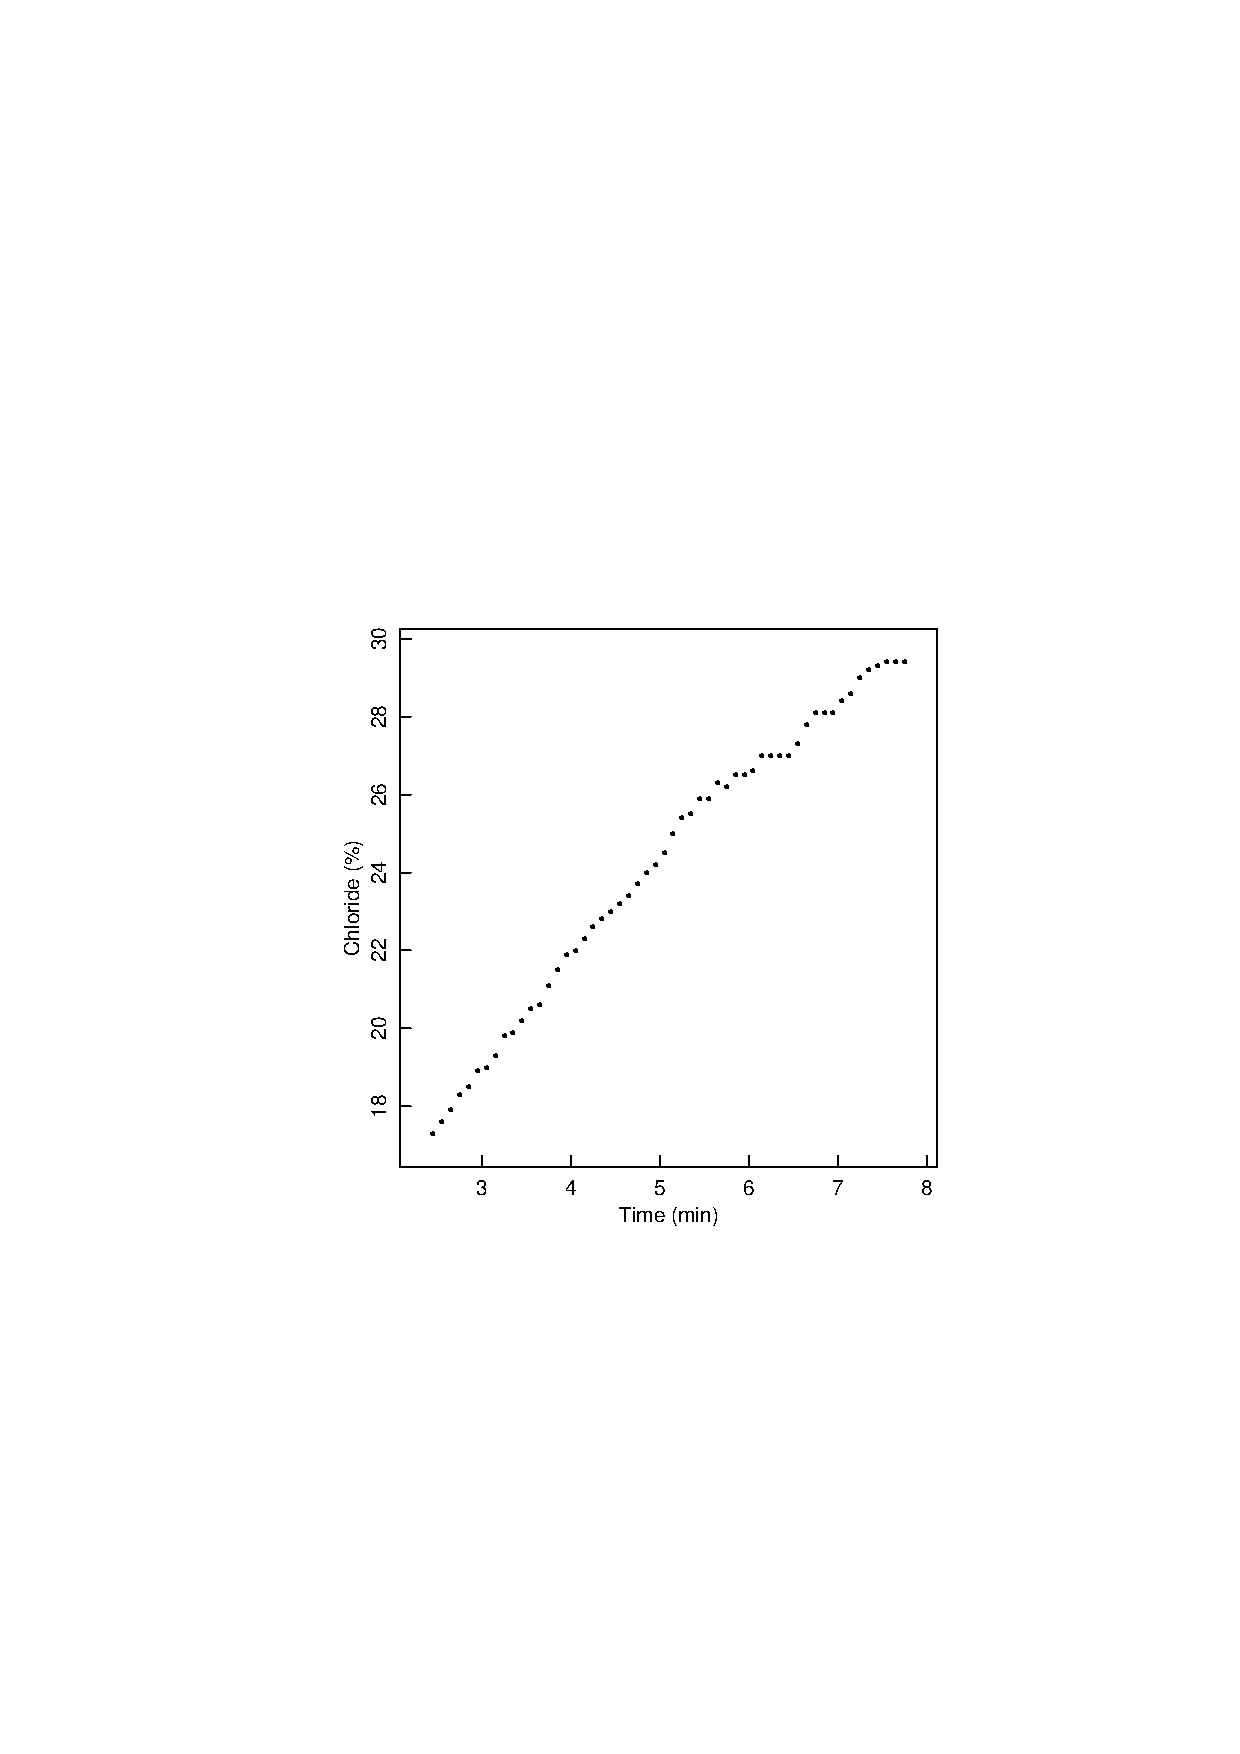
\includegraphics{3CHLdata}}%,height=3in}}
    \caption{Plot of chloride concentration versus time for the chloride
    transport data.}
    \label{fig:CHLdata}
  \end{figure}
The observation $y_{n}$ gives the chloride
concentration (in percent) at time $x_{n}$ (in minutes).

The model function
\begin{displaymath}
f ( x_n , \btheta ) = \theta_1
( 1 - \theta_2 e^{ - \theta_3 x_n } )
\end{displaymath}
was derived from the theory of ion transport,
where $\theta_{1}$ represents the final percentage
concentration of chlorine, $\theta_{3}$ is a rate constant,
and $\theta_{2}$ accounts for the
unknown initial and final concentrations of the chlorine and
the unknown initial reaction time.
As usual, it was assumed that the disturbances had zero mean and
constant variance and were independent.

An initial estimate for $\theta_{1}$ was obtained by
extrapolating the data to large time, giving
$\theta_1^0 = 35$.
Dividing $y_n $ by $\theta_1^{0}$ and linearizing
the equation by rearranging terms and taking logarithms
allowed us to estimate the remaining parameters by linear
regression, to give
$\btheta^0 = (35, 0.91, 0.22) \trans$.
Convergence was obtained to
$\hat{\btheta}= (39.09, 0.828,0.159)\trans$
with a residual sum of squares of 1.88.
\begin{figure}
  \vspace{2.25in}
  \centerline{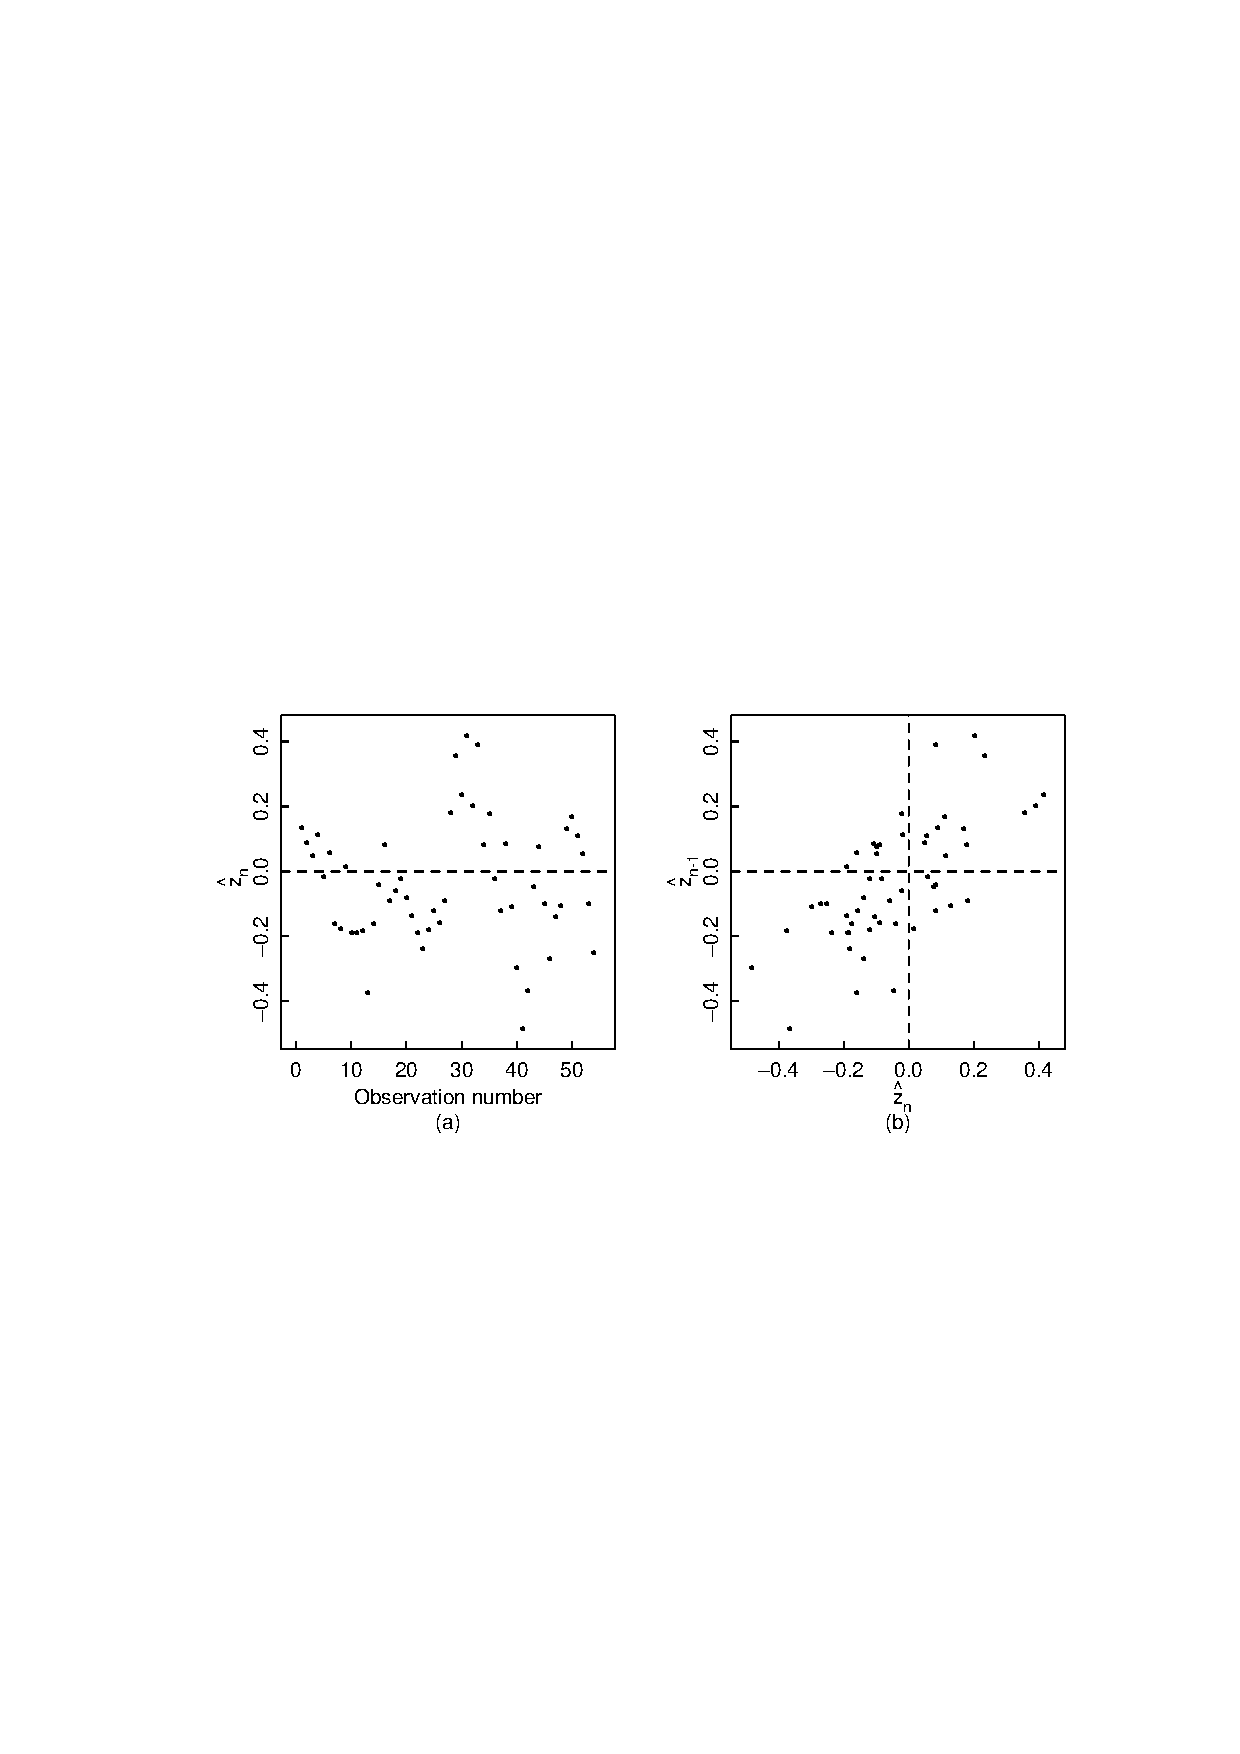
\includegraphics{3CHLres1}}%,height=2.25in}}
  \caption{Plots of the residuals $\hat z$ from the original nonlinear
    least squares fit to the chloride data.  The residuals are plotted
    as a time series in part $a$ and as a lag plot in part $b$.}
  \label{fig:CHLres1}
  \end{figure}
A time series plot of the residuals, shown in Figure~\ref{fig:CHLres1}$a$,
shows runs in the residuals.
Similarly, the lag plot shown in Figure~\ref{fig:CHLres1}$b$,
shows positive correlation.
We are thus alerted to the possibility that the disturbances are
not independent, or that there is some deficiency in the form of
the expectation function.
\end{example}

When the disturbances are not independent, the
model for the observations must be altered to account for
dependence.
Common forms for dependence, or \emph{autocorrelation}, of
\index{autocorrelation!of residuals}
disturbances are \emph{moving average}
or \emph{autoregressive}
\index{time series!moving average model}
\index{time series!autoregressive model}
models of variable order \cite{box:jenk:1976}.
%\glossary{ Box, G.E.P.}
%\glossary{ Jenkins, G.M.}
Simple examples of such forms are a moving average process of
order 1 where
\begin{displaymath}
Z_n = \epsilon_n - \omega_1 \epsilon_{n-1}
\end{displaymath}
or an autoregressive process of order 1 where
\begin{displaymath}
Z_n = \epsilon_n + \phi_1 Z_{n-1}
\end{displaymath}
and the $\epsilon_n , n = 1, 2 ,\ldots, N$, are independent random
disturbances with zero mean and constant variance,
or more simply, \emph{white noise}.

In regression situations,
when the data are equally spaced in time, it is relatively easy
to determine an appropriate form for the dependence of the
disturbances by calculating and plotting the \emph{residual
autocorrelation function},
\index{residual!autocorrelation function}
\begin{displaymath}
r_k = \sum_{n=k+1}^N
\frac{\hat z_n\hat z_{n-k}}{N s^2}   
k = 1,  2,\ldots
\end{displaymath}
versus the lag $k$.
In the definition of $r_{k}$, $s^{2}$ is the
variance estimate,
and the residuals are assumed to have zero average.
The residual autocorrelation function is usually calculated
out to $ k  \approx  N / 5 $.
If the residual autocorrelation function is consistently within
the range $\pm 2 / \sqrt N $ after lag 2 or 3, then
the model may be identified as a moving average process of order
1 or 2.
If the residual autocorrelation function tends to decay gradually
to zero, then the process may be identified as an autoregressive
process.
Alternatively, to determine the order of the autoregressive
process, it may be necessary to calculate the
\emph{partial autocorrelation function}
\cite{box:jenk:1976}.
%\glossary{ Box, G.E.P.}
%\glossary{ Jenkins, G.M.}
\index{partial autocorrelation function}
For regression situations where time is not the only
factor, or the most important factor, first order
autoregressive processes are often adequate.

\begin{example}\label{chlor:2}

The residual autocorrelation function for the chloride
  \begin{figure}
    \vspace{2.25in}
    \centerline{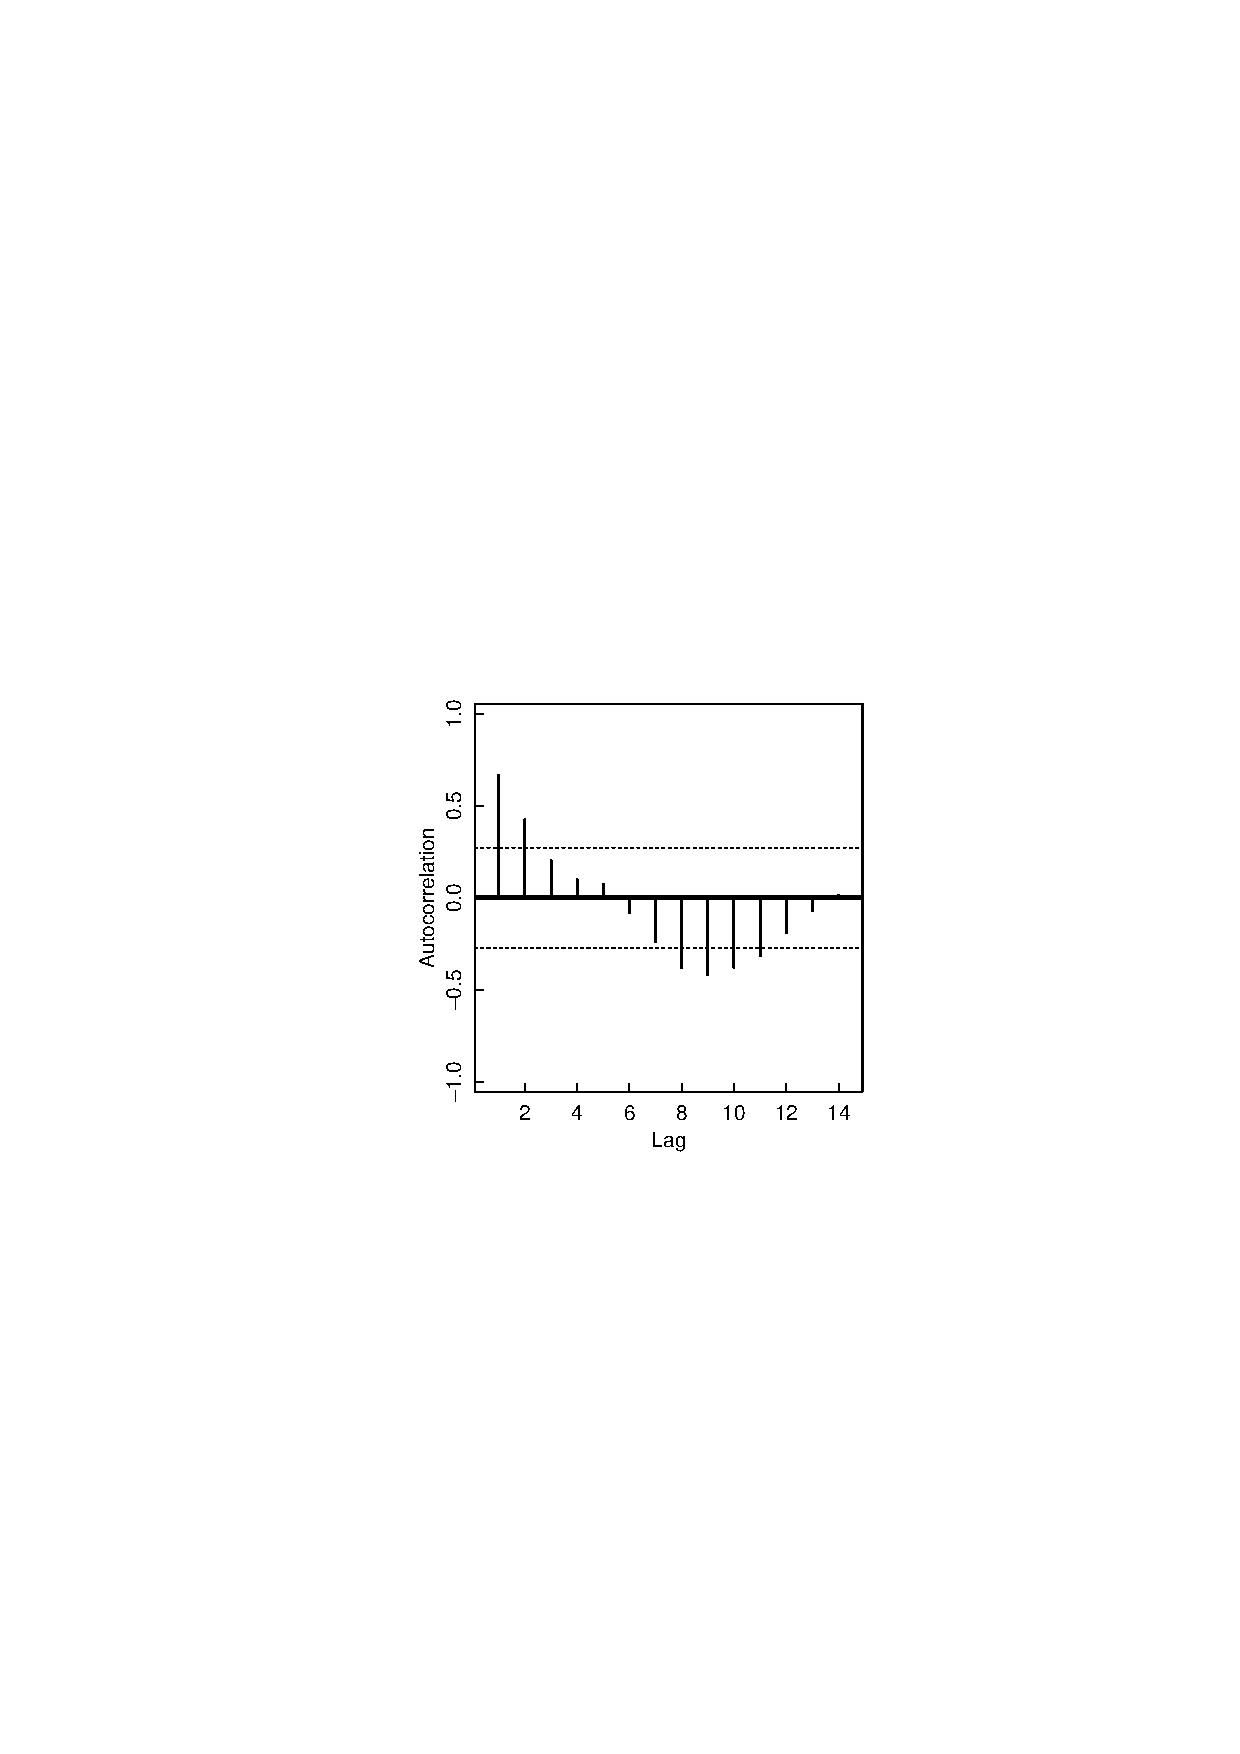
\includegraphics{3CHLauto}}%,height=2.25in}}
    \caption{
    Autocorrelation function of the residuals from the original nonlinear
    least squares fit to the chloride data.
    The dotted lines enclose the interval in which approximately 95\% of
    the correlations would be expected to lie if the true correlations
    were 0.
    }\label{fig:CHLauto}
  \end{figure}
data was calculated and plotted as in Figure \ref{fig:CHLauto}.
The correlation estimates decay towards zero, falling within
the limits $\pm 2 / \sqrt N$ (shown as dotted horizontal
lines) quite quickly.
On the basis of this plot, it was decided that a first order
autoregressive
process would adequately model the dependence in the residuals.

The model to be fitted is now of the form
$Y_n = f ( x_n , \btheta ) + Z_{n}$, where
$Z_n = \epsilon_n + \phi  Z_{n-1}$.
To estimate the parameters $\btheta$ and $\phi$, we
reduce the problem to an ordinary nonlinear least
squares problem by subtracting $\phi$ times the equation for
$Y_{n-1}$ from $Y_{n}$, as
\begin{displaymath}
Y_n - \phi Y_{n-1} =
f ( x_n , \btheta ) - \phi 
f ( x_{n-1} , \btheta ) + Z_n - \phi  Z_{n-1}
\end{displaymath}
or
\begin{displaymath}
Y_n = \phi Y_{n-1} +
f ( x_n , \btheta ) - \phi  f ( x_{n-1} , \btheta ) + \epsilon_n
\end{displaymath}

Starting values for $\btheta$ were taken from $\hat{\btheta}$
above, and the starting value for $\phi$ was taken as the lag
one correlation estimate, $r_1 = 0.67$.
Convergence was obtained to
$( \btheta \trans , \phi ) = ( 37.58,  0.849,  0.178,  0.69 )$
with a residual sum of squares of 0.98.
The residuals $\hat \epsilon$ from this fit are
\begin{figure}
  \centerline{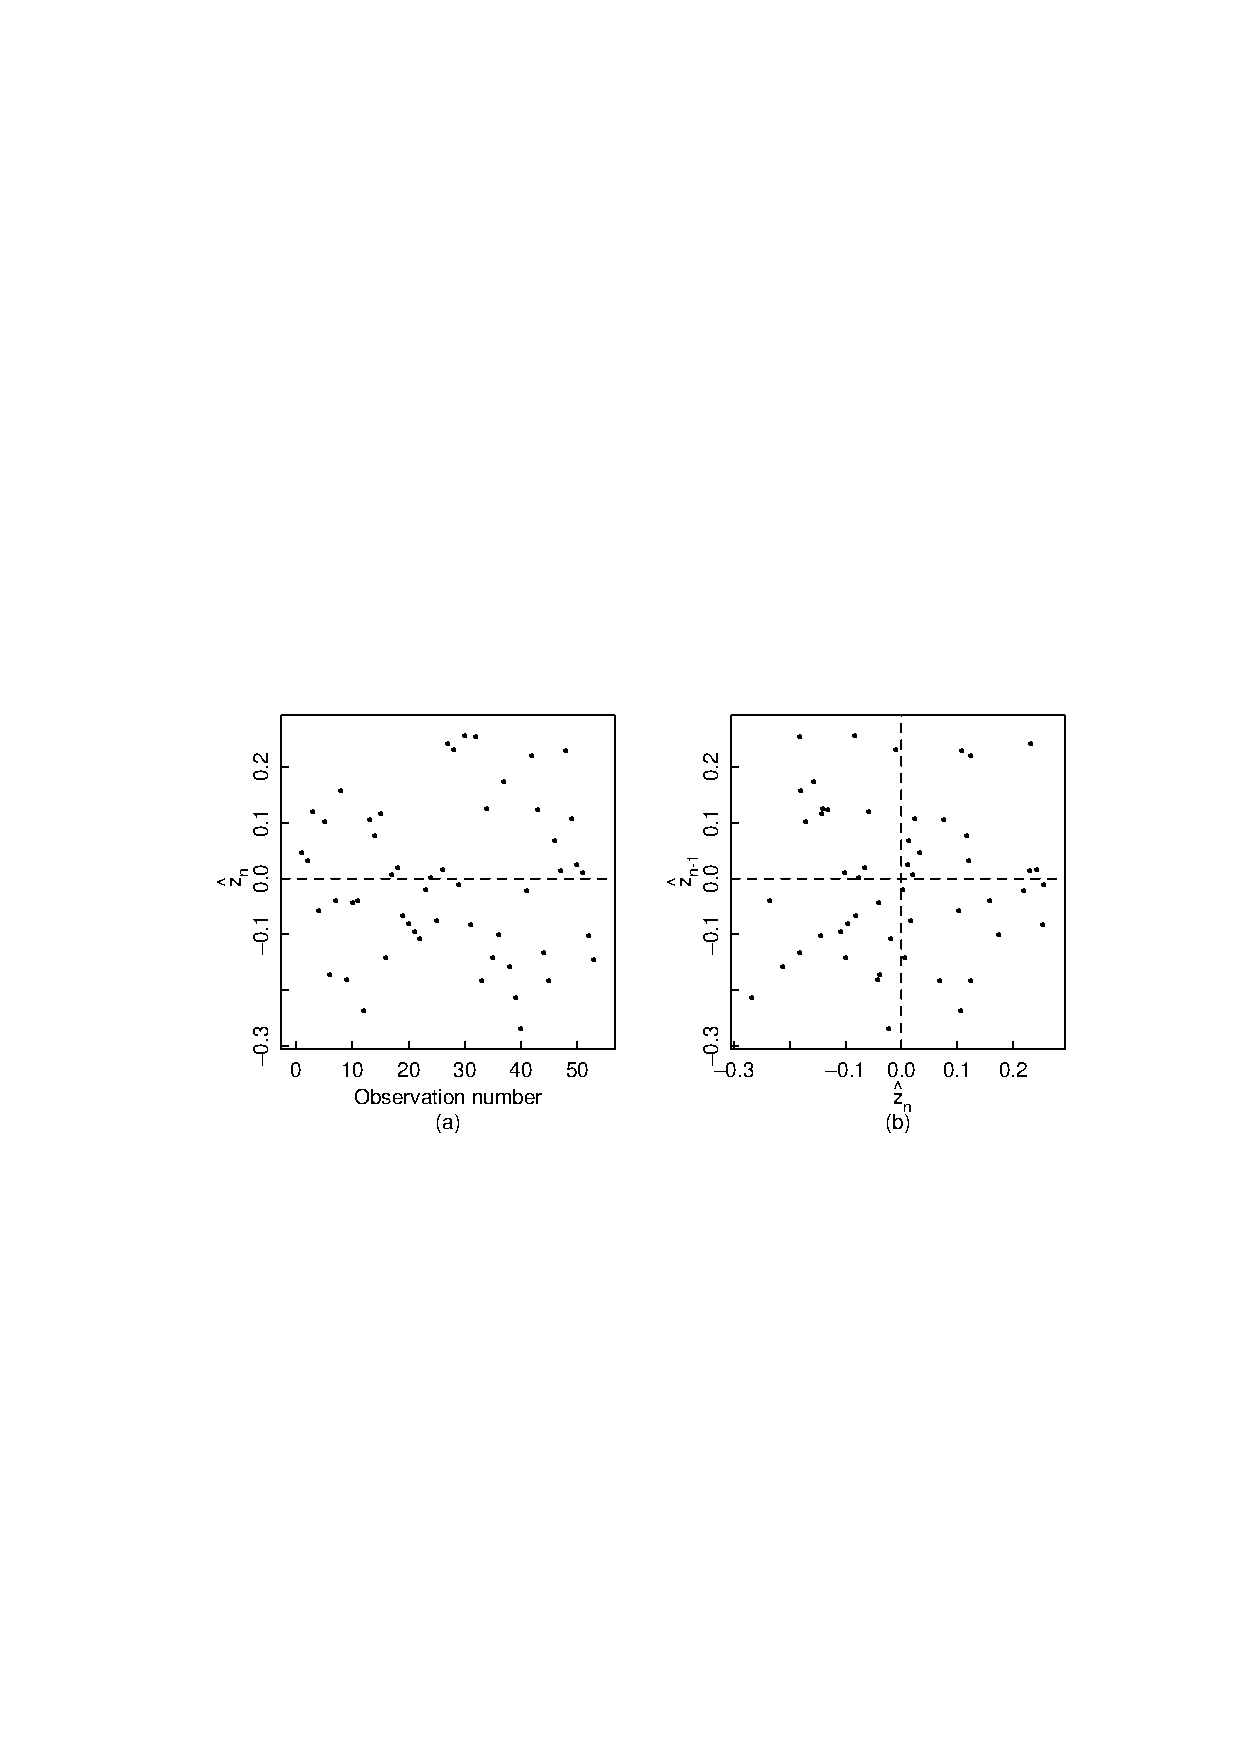
\includegraphics{3CHLres2}}%,height=2.25in}}
  \caption{Plots of the residuals $\hat z$ from the nonlinear least
    squares fit to the chloride data using $\phi=0.69$.  The residuals
    are plotted as a time series in part $a$ and as a lag plot in part
    $b$.}
  \label{fig:CHLres2}
\end{figure}
well behaved, as shown in Figure \ref{fig:CHLres2} and
\begin{figure}
  \centerline{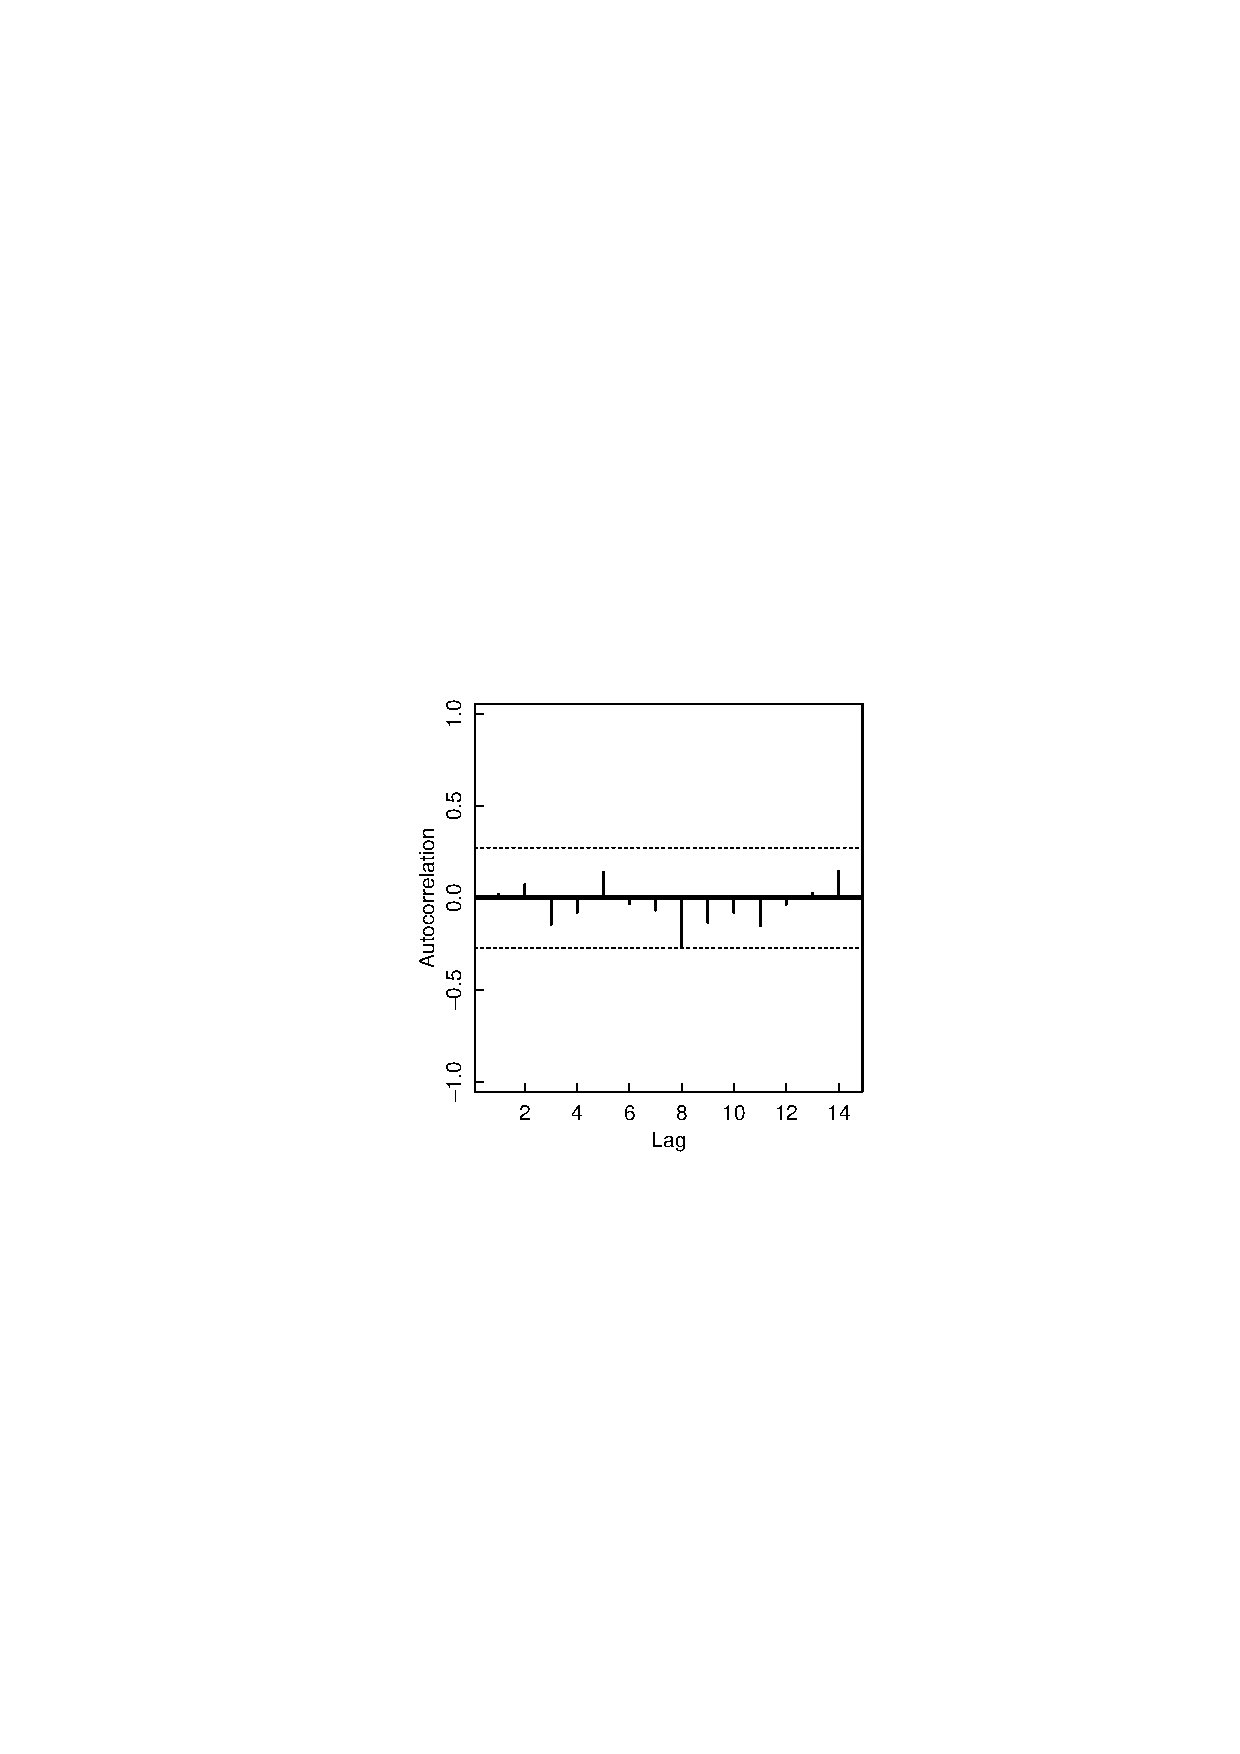
\includegraphics{3CHLacf2}}%,height=2.25in}}
  \caption{Autocorrelation function of the residuals from the nonlinear
    least squares fit to the chloride data using $\phi=0.69$.  The
    dotted lines enclose the interval in which approximately 95\% of
    the correlations would be expected to lie if the true correlations
    were 0.}
  \label{fig:CHLacf2}
  \end{figure}
the residual autocorrelation function, shown in Figure
\ref{fig:CHLacf2}, was uniformly small.
\end{example}

In general, as in the above example,
the main effect of accounting for dependence is to
reduce the residual variance and reduce the correlation in
the residuals: the model parameter estimate
$\hat{\btheta}$ does not change much.
However, the model parameters are better estimated
because they have smaller standard errors and because the
method of least squares has been applied correctly,
since the assumptions are satisfied.
For a more complicated application of this technique, see
\citeasnoun{watt:baco:1974}.
%\glossary{ Watts, D.G.}
%\glossary{ Bacon, D.W.}

\section{Accumulated Data}
\index{practical considerations!accumulated data}
\index{accumulated data}

In some studies, when it is impractical to measure instantaneous
concentrations, \emph{accumulated}
responses are recorded.
\label{eth:1}
\begin{example}

An experiment to study the metabolism of ethyl acrylate was
performed by giving rats a single bolus of radioactively tagged
ethyl acrylate.
Each rat was given a measured dose of the compound via stomach
intubation and placed in an enclosed cage from which the air
could be drawn through a bubble chamber.
The exhaled air was bubbled through the chamber, and at a
specified time the bubble chamber was replaced by a fresh one, so
that the measured response was the accumulated CO$_{2}$ during
the time interval.
Preliminary analysis of the data revealed that normalizing each
animal's response by dividing by the actual dose received would
permit combination of the data so that a single model could be
fitted to the data for all the rats.
Furthermore, the variability in the normalized data was such that
it was necessary to take logarithms of the data to produce
constant variance across the time points.
The starting points and lengths of the accumulation intervals and the
averages for the nine rats, normalized by actual dose, are given
in Appendix~\ref{atbl:co2} \cite{watt:debe:stir:1986}, and
%\glossary{ Watts, D.G.}
%\glossary{ deBethizy, D.}
%\glossary{ Stiratelli, R.G.}
the cumulative CO$_{2}$ data are plotted
in Figure \ref{fig:CO2data}.
\begin{figure}
  \centerline{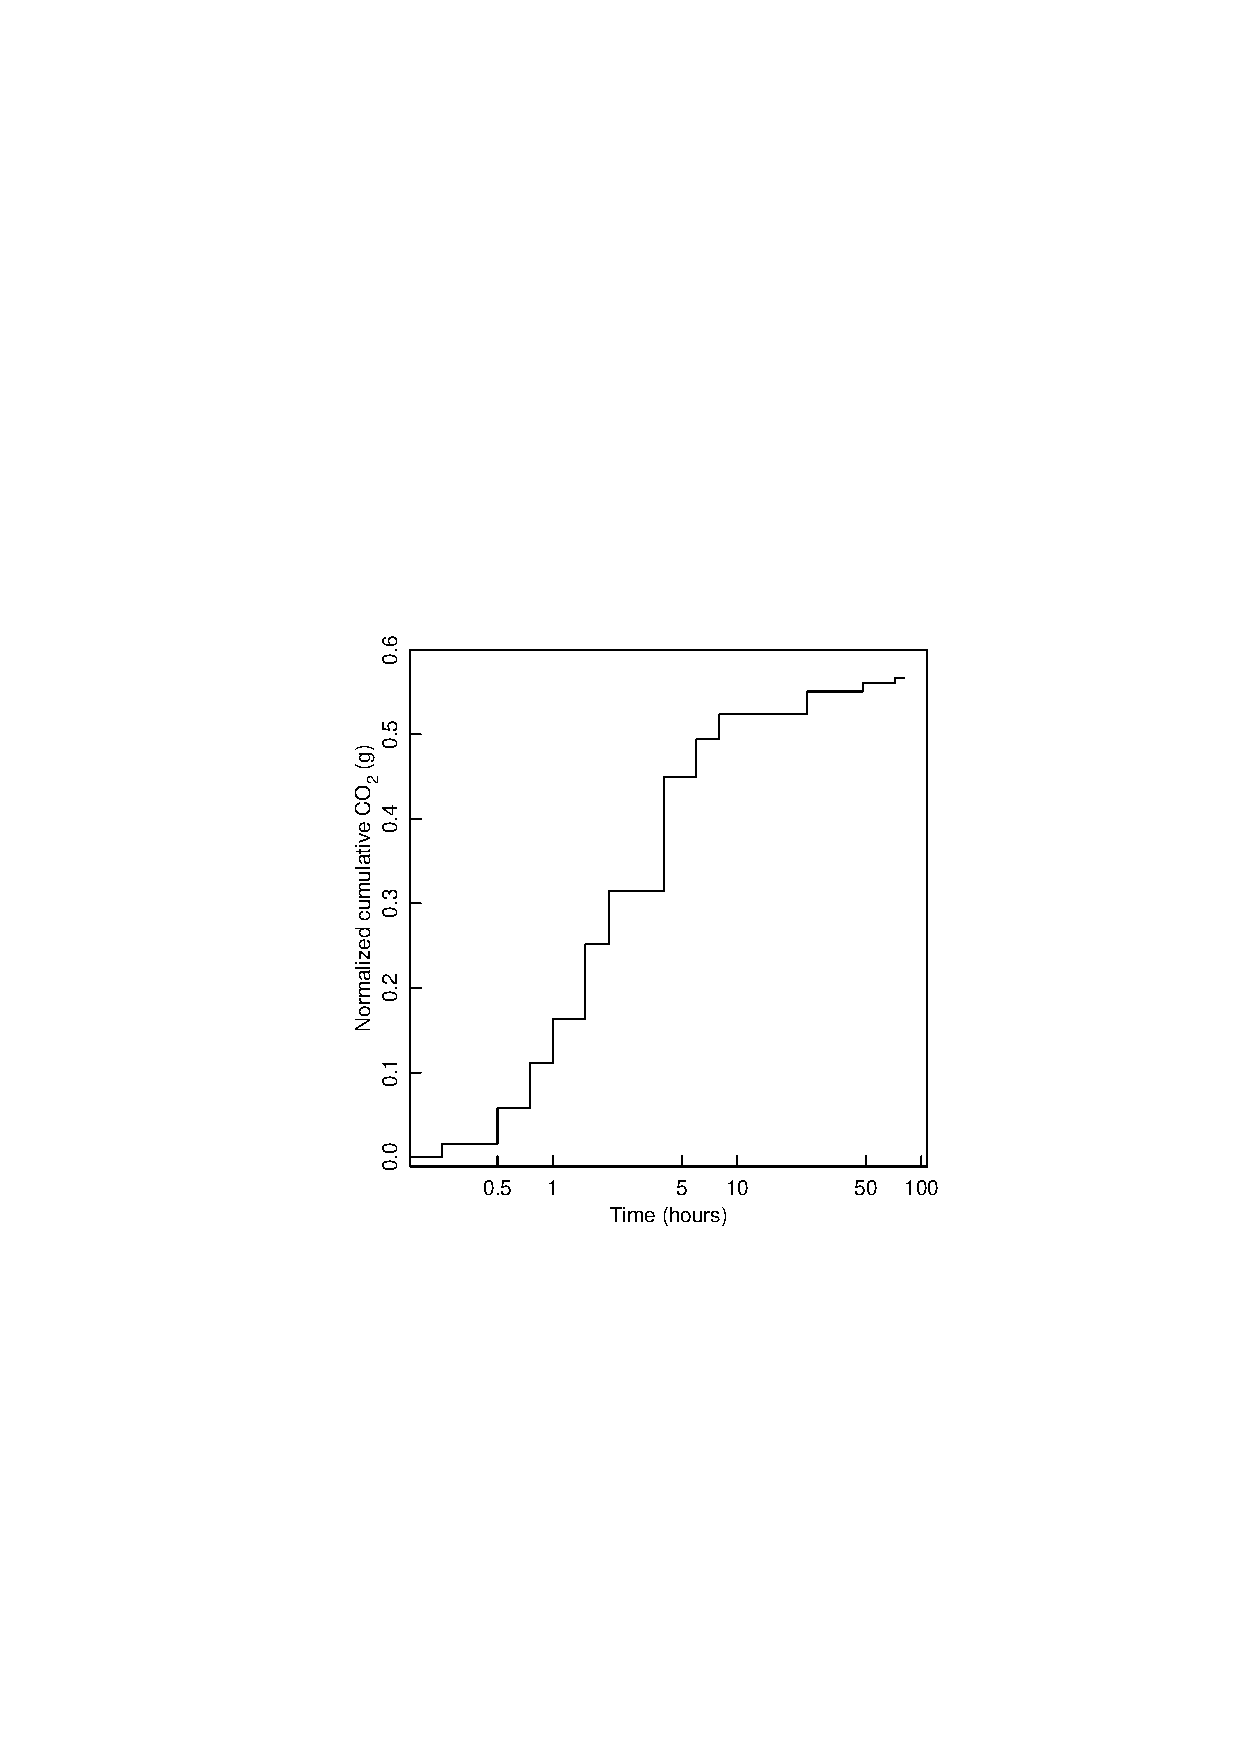
\includegraphics{3CO2data}}%,height=3in}}
  \caption{Plot of cumulative exhaled CO$_{2}$ amounts versus
    collection interval end point for the ethyl acrylate data.}
  \label{fig:CO2data}
  \end{figure}
\end{example}

Two methods for the analysis of such data were given in \citeasnoun{renw:1982}.
%\glossary{ Renwick, A.G.}
The first method uses peeling of the ``approximate concentration''
data obtained by dividing the accumulated amount by
the accumulation time interval.
The second method
uses the cumulative total, extrapolated to infinite time,
and then peeling of the differences
\index{peeling}
$[ extrapolated - (cumulative  total)]$.
This is called the ``sigma-minus''
\index{sigma-minus method!for accumulated data}
method.

We do not recommend either of these methods, and specifically
decry use of the sigma--minus method because it is so sensitive
to variations in the extrapolated value.
It can be shown, for example, that small percentage changes in the
extrapolated value, say less than 2\%, can cause
changes in the rate constants in excess of 100\%.
Furthermore, both methods are based on peeling, which requires
excessive subjective judgement.
Instead of the abovementioned methods, we recommend direct
analysis of the accumulated data using integrated responses
as described below.
In addition to avoiding the disadvantages of the other methods, this
method has the advantage that it provides measures of precision of the
estimates in the form of parameter approximate standard errors and
correlations.

\subsection{Estimating the Parameters by Direct Integration}
\index{accumulated data!analysis by direct integration}

Suppose that the theoretical response to the input stimulus at time
$t$ is $f ( t, \btheta )$.
Then the accumulated output in the interval
$t_{n-1}$ to $t_{n}$ is
\begin{displaymath}
F_n =
\int_{t_{n-1}}^{t_n} f(t,\btheta) dt
\end{displaymath}
We therefore use the integrated function values $F_n $ and the observed
accumulated data pairs $( y_n ,t_n )$ to estimate the
parameters.
We rewrite the model in terms of the factors $x_{1n}=t_{n-1}$,
the start of the interval, and $x_{2n}=t_n-t_{n-1}$, the
length of the interval, so the model for the amount accumulated in an
interval is $F(\bx_n,\btheta)$, where
$\bx_n=(x_{1n},x_{2n})\trans$.

To determine a tentative form for $f ( t , \btheta )$, we plot the
approximate rates
${y_n} / {x_{2n}}$ versus
$x_{1n}+x_{2n} / 2$ on semilog paper and use peeling to
obtain \emph{starting} estimates for the parameters.
The final estimation is done using nonlinear least squares.
Note that if the variance is not constant, it may be necessary to
transform the data and the function, as in the following example.

\begin{example}\label{eth:2}
  The CO$_{2}$ data are reproduced in Table~\ref{tbl:CO2rate} together
  with the derived quantities (interval midpoint
  $x_{1n}+ x_{2n} / 2$ and approximate rate
  $y_n / x_{2n}$) which are plotted in Figure~\ref{fig:CO2apconc}.
  \begin{table}
    \caption{
      Collection intervals and averages of normalized exhaled CO$_{2}$
      for the ethyl acrylate data together with the derived quantities:
      interval midpoint and approximate rate }\label{tbl:CO2rate}
    \begin{center}
      \begin{tabular}{cclll} \hline
        \multicolumn{2}{c}{Collection} & &
        \multicolumn{2}{c}{Derived}\\ \multicolumn{2}{c}{Interval (hr)} &
        & \multicolumn{2}{c}{Quantities}\\ \multicolumn{1}{c}{Start} &
        \multicolumn{1}{c}{Length} & \multicolumn{1}{c}{CO$_{2}$} &
        \multicolumn{1}{c}{Interval} & \multicolumn{1}{c}{Approx.}\\
        \multicolumn{1}{c}{$x_{1}$} & {$x_{2}$} & \multicolumn{1}{c}{(g)}
        & \multicolumn{1}{c}{Midpoint} & \multicolumn{1}{c}{Rate}\\ \hline
        0.0&0.25&0.01563&0.125&0.0625\\ 0.25&0.25&0.04190&0.375&0.1676\\
        0.5&0.25&0.05328&0.625&0.2131\\ 0.75&0.25&0.05226&0.875&0.2090\\
        1.0&0.5&0.08850&1.25&0.1770\\ 1.5&0.5&0.06340&1.75&0.1268\\
        2.0&2.0&0.13419&3.0&0.0671\\ 4.0&2.0&0.04502&5.0&0.0225\\
        6.0&2.0&0.02942&7.0&0.0147\\ 8.0&16.0&0.02716&16.0&0.0017\\
        24.0&24.0&0.01037&36.0&0.0004\\ 48.0&24.0&0.00602&60.0&0.0003\\
        \hline
      \end{tabular}
    \end{center}
  \end{table}
  \begin{figure}
    \centerline{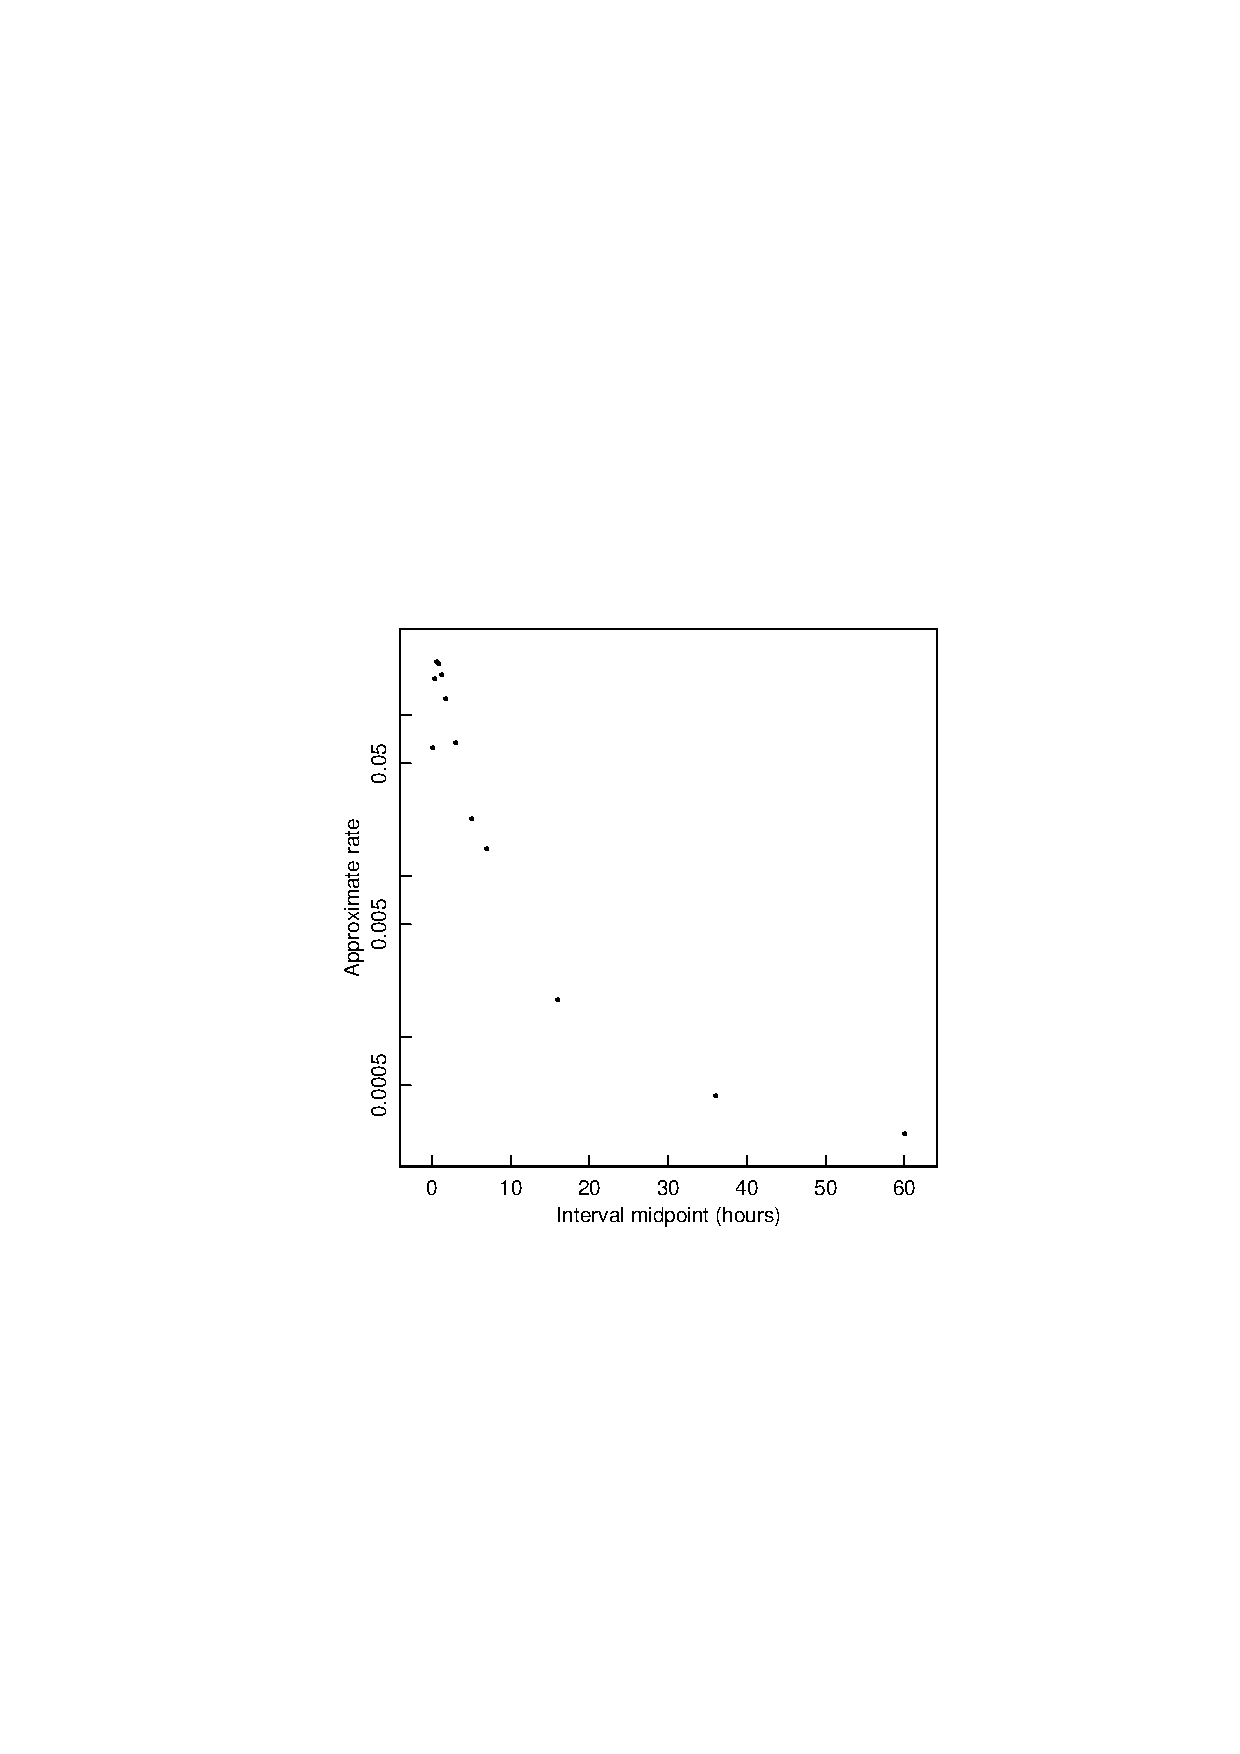
\includegraphics{3CO2apconc}}%,height=3in}}
    \caption{Approximate CO$_{2}$ exhalation rate versus collection
      interval midpoint for the ethyl acrylate data.}
    \label{fig:CO2apconc}
  \end{figure}
  We can see from the figure that an
  appropriate model for the data involves three exponentials
  (two to account for the peak, and another to account for the
  change in slope of the decay from the peak).
  Because the radioactivity prior to injection must be zero,
  the concentration at $ t = 0$ must be zero.
  A plausible model for the concentration at time $t$ is therefore
  \begin{displaymath}
    f(t, \btheta )=- ( \theta_4 + \theta_5 ) e^{ - \theta_1 t }
    + \theta_4 e^{{-} \theta_2 t }
    + \theta_5 e^{{-} \theta_3 t }
  \end{displaymath}
  An appropriate model for the accumulated data in the
  collection interval starting at $t_{n-1} $ is then
  \begin{eqnarray*}
    F_n&=&-\frac{\theta_4+\theta_5}{\theta_1}( e^{ - \theta_1 t_{n-1} } -
    e^{ - \theta_1 t_n } )\\
    &&+\frac{\theta_4}{\theta_2}(e^{-\theta_2 t_{n-1} }-e^{-\theta_2 t_n})
    +\frac{\theta_5}{\theta_3}
    ( e^{{-} \theta_3 t_{n-1} } - e^{{-} \theta_3 t_n} )
  \end{eqnarray*}
  or
  \begin{eqnarray*}
    F(\bx,\btheta)&=&
    -\frac{\theta_4+\theta_5}{\theta_1}e^{-\theta_1 x_1}(1-e^{-\theta_1 x_2})\\
    &&+\frac{\theta_4}{\theta_2}e^{-\theta_2 x_1}(1-e^{-\theta_2 x_2})
    +\frac{\theta_5}{\theta_3}e^{-\theta_3 x_1}(1-e^{-\theta_3 x_2})
  \end{eqnarray*}
  Because of the nonconstant variance, the logarithms of $F$ were
  fitted to the logarithms of the data.
  The results of this analysis together with the starting estimates
  are presented
  in Table~\ref{tbl:5.2}.
  \begin{table}
    \caption{
      Parameter summary for the 3-exponential model fitted to the
      ethyl acrylate data.}\label{tbl:5.2}
    \begin{center}
      \begin{tabular}{cllc}\hline
        & & \multicolumn{2}{c}{Nonlinear Least Squares}\\ & & &
        \multicolumn{1}{c}{Approx.}\\ \multicolumn{1}{c}{Parameter} &
        \multicolumn{1}{c}{Start} & \multicolumn{1}{c}{Estimate} &
        \multicolumn{1}{c}{Std. Err.}\\ \hline
        $\theta_{1}$&4.461&3.025&0.752\\ $\theta_{2}$&0.571&0.481&0.038\\
        $\theta_{3}$&0.0434&0.0258&0.0096\\ $\theta_{4}$&0.355&0.310&0.049\\
        $\theta_{5}$&0.0034&0.0011&0.0005\\ \hline
      \end{tabular}
    \end{center}
  \end{table}
  In an analysis of the logarithmic data for the individual rats, due
  attention was paid to the behavior of the residuals.
  The triple rate constant model fitted the data very well.
\end{example}

\begin{example}\label{sac:1}
  As a second example of treating accumulated data,
  we analyze the saccharin data in \citeasnoun{renw:1982}.
  % \glossary{ Renwick, A.G.}
  In this experiment, the measured response was the amount of
  saccharin accumulated in the urine of a rat after receiving a
  single bolus of saccharin.
  The data are recorded in Appendix~\ref{atbl:sac}, and plotted
  in Figure~\ref{fig:SACdata}.
  \begin{figure}
    \centerline{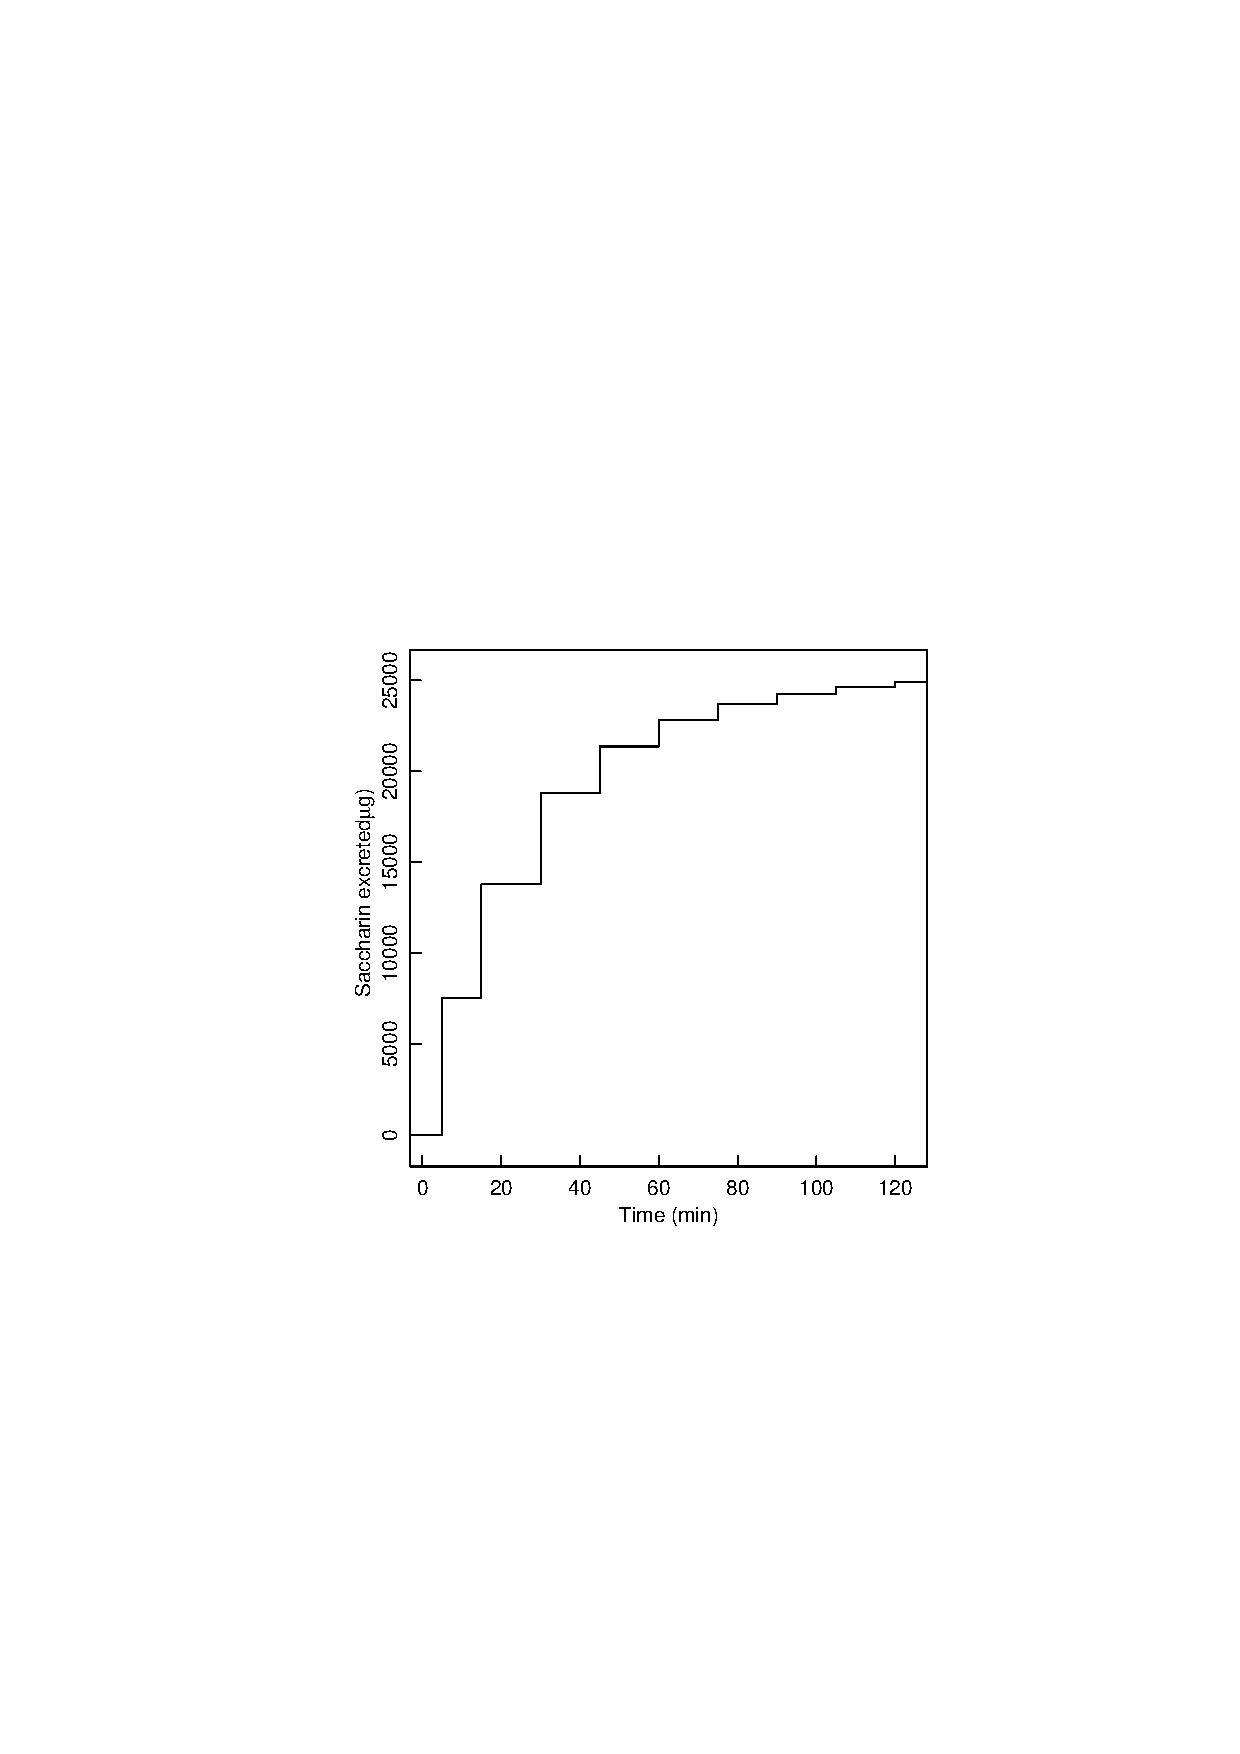
\includegraphics{3SACdata}}%,height=3in}}
    \caption{Plot of cumulative excreted amount versus collection
      interval end point for the saccharin data.}
    \label{fig:SACdata}
  \end{figure}
  
  The function involved only two rate constants, and the
  response was modeled as
  \begin{displaymath}
    f(t, \btheta ) = \theta_3 e^{ - \theta_1 t }
    + \theta_4 e^{{-} \theta_2 t }
  \end{displaymath}
  so
  \begin{displaymath}
    F(\bx,\btheta)=\frac{\theta_3}{\theta_1}e^{-\theta_1 x_1}
    ( 1 - e^{ - \theta_1 x_2} )
    +\frac{\theta_4}{\theta_2}
    e^{ - \theta_2 x_1 }
    ( 1 - e^{ - \theta_2 x_2} )
  \end{displaymath}
  As in the ethyl acrylate example, the integrated model was fitted to
  the logarithms of the accumulated data to stabilize
  variance.
  
  The curve peeling and the sigma--minus method results from \citeasnoun{renw:1982}
  % \glossary{ Renwick, A.G.}
  are given in columns 2 and 3 of
  Table \ref{tbl:3}, and the
  results using the direct integration method are given in column 4.
  \begin{table}
    \caption{
      Parameter summary for the saccharin data, comparing estimates
      obtained using the sigma--minus method, using the approximate rate
      method, and using nonlinear least squares to fit the integrated
      response function.  }\label{tbl:3}
    \begin{center}
      \begin{tabular}{clclc} \hline
        \multicolumn{5}{c}{Estimate by}\\ & & &
        \multicolumn{2}{c}{Nonlinear Least Squares}\\ & & & &
        \multicolumn{1}{c}{Approx.}\\ \multicolumn{1}{c}{Parameter} &
        \multicolumn{1}{c}{Peeling$^{a}$} &
        \multicolumn{1}{c}{Sigma--Minus$^{a}$} & \multicolumn{1}{c}{Value}
        & \multicolumn{1}{c}{Std. Err.}\\ \hline
        $\theta_{1}$&0.0710&0.0833&0.122&0.031\\
        $\theta_{2}$&0.0234&0.0255&0.0279&0.003\\
        $\theta_{3}$&830&932&1345&249\\
        $\theta_{4}$&270&314&402&98\\
        \hline
      \end{tabular}
    \end{center}
     $^{a}$ From \citeasnoun{renw:1982}.
%\glossary{ Renwick, A.G.}
   \end{table}
  
  Note the considerable differences between the results based on
  peeling and those obtained by nonlinear least squares.
  Note too, that the peeling and sigma--minus methods do not
  provide parameter standard errors.
  
  There were two very large residuals from the nonlinear least
  squares fit, at $x_1=5$ and $x_1=105$.
  A second analysis was done by simply combining the observations
  at $x_1=5$ and  $x_1=15$ and at
  $x_1=90$ and $x_1=105$, as shown in Table \ref{tbl:SACHed}.
  \begin{table}
    \caption{
      Collection intervals and excreted amounts for original and
      combined saccharin data.  }\label{tbl:SACHed}
    \begin{center}
      \begin{tabular}{cccccc} \hline
        \multicolumn{3}{c}{Original} & \multicolumn{3}{c}{Combined}\\
        \hline \multicolumn{2}{c}{Collection} & &
        \multicolumn{2}{c}{Collection} &\\ \multicolumn{2}{c}{Interval (hr)}
        & & \multicolumn{2}{c}{Interval (hr)} & \\ \multicolumn{1}{c}{Start}
        & \multicolumn{1}{c}{Length} & \multicolumn{1}{c}{Saccharin} &
        \multicolumn{1}{c}{Start} & \multicolumn{1}{c}{Length} &
        \multicolumn{1}{c}{Saccharin}\\ \multicolumn{1}{c}{$x_{1}$} &
        \multicolumn{1}{c}{$x_{2}$} & \multicolumn{1}{c}{$(\mu$g)} &
        \multicolumn{1}{c}{$x_{1}$} & \multicolumn{1}{c}{$x_{2}$} &
        \multicolumn{1}{c}{$(\mu$g)}\\ \hline 0&5&7518&0&5&7518\\
        5&10&6275&5&25&11264\\ 15&15&4989&\\ 30&15&2580&30&15&2580\\
        45&15&1485&45&15&1485\\ 60&15&861&60&15&861\\ 75&15&561&75&15&561\\
        90&15&363&90&30&663\\ 105&15&300\\ \hline
      \end{tabular}
    \end{center}
  \end{table}
  
  The residuals from this fit were very well behaved, and the
  residual variance was reduced to 0.0071 from 0.0158.
  The parameter estimates (standard errors in parentheses) were
  $\theta_1 = 0.154 (0.035)$,
  $\theta_2 = 0.030 (0.002)$,
  $\theta_3 = 1506  (233)$, and
  $\theta_4 =  472 (70)$.
\end{example}

\section{Comparing Models}
\index{practical considerations!comparing models}

In some situations there may be more than one function
which could be used as a model.
For example, in fitting a double exponential model,
\begin{displaymath}
  f ( x , \btheta ) = \theta_1 e^{ - \theta_2 x } +
  \theta_3 e^{ - \theta_4 x}
\end{displaymath}
$\theta_{4}$ could be $0$, in which case the model reduces to
\begin{displaymath}
  f ( x , \btheta ) = \theta_1 e^{ - \theta_2 x } + \theta_3
\end{displaymath}
or $\theta_{3}$ could be 0, in which case the model reduces to
\begin{displaymath}
  f ( x , \btheta ) = \theta_1 e^{ - \theta_2 x }
\end{displaymath}
In this situation of \emph{nested} models, we would be
\index{nested model}
\index{model!nested}
interested in finding the simplest model which adequately fits the data.

In other situations, we might compare \emph{non-nested}
\index{model!non-nested}
models---for example, model 1
\begin{displaymath}
  f ( x , \btheta ) = \theta_1 ( 1 - e^{ - \theta_2 x } )
\end{displaymath}
versus model 2
\begin{displaymath}
  f ( x , \btheta )=\frac{\theta_1x}{\theta_2+x}
\end{displaymath}
both of which start at $f=0$ when $x=0$ and approach the
asymptote $\theta_{1}$ as $x\to\infty$.
In these situations, one model may give a superior fit to the data,
and we would like to select that model.

\subsection{Nested Models}

To decide which is the simplest nested model to fit a
data set adequately, we proceed as in the linear case and use
a likelihood ratio test \cite{drap:smit:1998}.
Because of the spherical normal assumption, this leads to an
assessment of the extra sum of squares
\index{extra sum of squares!analysis for nested models}
\index{sum of squares!extra}
due to the extra parameters involved in
\index{parameter!extra degrees of freedom}
\index{degrees of freedom!extra parameter}
going from the partial to the full model.

Letting $S$ denote the sum of squares, $\nu$ the degrees of
freedom, and $P$ the number of parameters, with subscripts $f$
and $p$ for the \emph{full}
and \emph{partial} models and a subscript $e$
for \emph{extra},
the calculations can be summarized as in
Table~\ref{tbl:extra}.
\begin{table}
  \caption{Extra sum of squares analysis for nested models.}
  \label{tbl:extra}
  \begin{center}
    \begin{tabular}{c  c  c  c  c} \hline
      & \multicolumn{1}{c}{Sum of} & \multicolumn{1}{c}{Degrees of}
      &\multicolumn{1}{c}{Mean Square} & \multicolumn{1}{c}{F Ratio}\\
      \multicolumn{1}{c}{Source} & \multicolumn{1}{c}{Squares}
      &\multicolumn{1}{c}{Freedom} \\ \hline Extra parameters&$S_e = S_p -
      S_{f}$& $\nu_e = P_f - P_{p}$&$s_e^2 = S_e / \nu_{e}$&
      ${s_e^2}/{s_f^2}$\\ Full model&$S_{f}$&$\nu_f = N - P_{f}$& $s_f^2 =
      S_f / \nu_{f}$\\ \hline Partial model&$S_{p}$&$N - P_{p}$\\ \hline
    \end{tabular}
  \end{center}
\end{table}
To complete the analysis, we compare the ratio $s_e^2 / s_f^{2}$ to
$F(\nu_e,\nu_f;\alpha)$ and accept the 
partial model if the calculated mean square ratio is lower than the
table value.
Otherwise, we retain the extra terms and use the full model.
Illustrations of the use of the extra sum of squares analysis are
given below in Example Puromycin~\ref{mic:10} and in Section 3.11.

Note that for linear least squares, the extra sum of squares
analysis is exact because the
data vector $\by$ is being projected onto linear subspaces of the
response space to determine $S_{p}$ and $S_{f}$.
Mathematically, the partial model
expectation plane is a linear subspace of the full model
expectation plane.
Residual vectors can then be decomposed into orthogonal
components and, from the fact that the full model residual vector
has a squared length which is distributed as a
$\sigma^2 \chi^{2}$ random variable with $N - P$ degrees of
freedom, it follows that the squared lengths of the components
are also distributed as $\sigma^2 \chi^{2}$ random variables
with degrees of freedom equal to the dimensions of the linear
subspaces.

For nonlinear models, as we might expect, the analysis is only
approximate because the calculated mean square ratio will not have
an exact F distribution.
However, the distribution of the mean square ratio is only
affected by intrinsic nonlinearity and not by parameter effects
nonlinearity,
\index{extra sum of squares!and nonlinearity}
and, as shown in Chapter 7, the intrinsic nonlinearity is generally small.
When the partial model is inadequate,
the effect of intrinsic nonlinearity on the analysis can be large but the
partial model will be rejected anyway:
it is only when the fitted values are very close that the form of the
distribution is critical.
In these cases, the intrinsic nonlinearity will usually
have a small effect because the expected responses being compared are close
together on the expectation surface.
\subsection{Incremental Parameters and Indicator Variables}

Many nested models can be parametrized in terms of incremental
parameters.
An \emph{incremental parameter} accounts for a
\index{parameter!incremental}
\index{incremental!parameter}
change in a parameter between blocks of cases and is
associated with an indicator variable.
\index{indicator variable}
\index{variable!indicator}
An advantage of using incremental parameters is that a
preliminary evaluation of the need for the full model can
be made directly from the regression output without having
to do additional computation.
The use of incremental parameters is most easily described by
means of an example.

\begin{example}
  \label{mic:10}
  In the Puromycin experiment, two blocks of experiments were run.
  In one the enzyme was treated with puromycin (Table A1.3$a$), and
  in the other the same enzyme was untreated
  (Table A1.3$b$).
  It was hypothesized that the Puromycin should affect the maximum
  velocity parameter $\theta_{1}$, but not the half-velocity
  parameter $\theta_{2}$.
  The two data sets are plotted in
  Figure~\ref{fig:MIC2data}.
  \begin{figure}
    \centerline{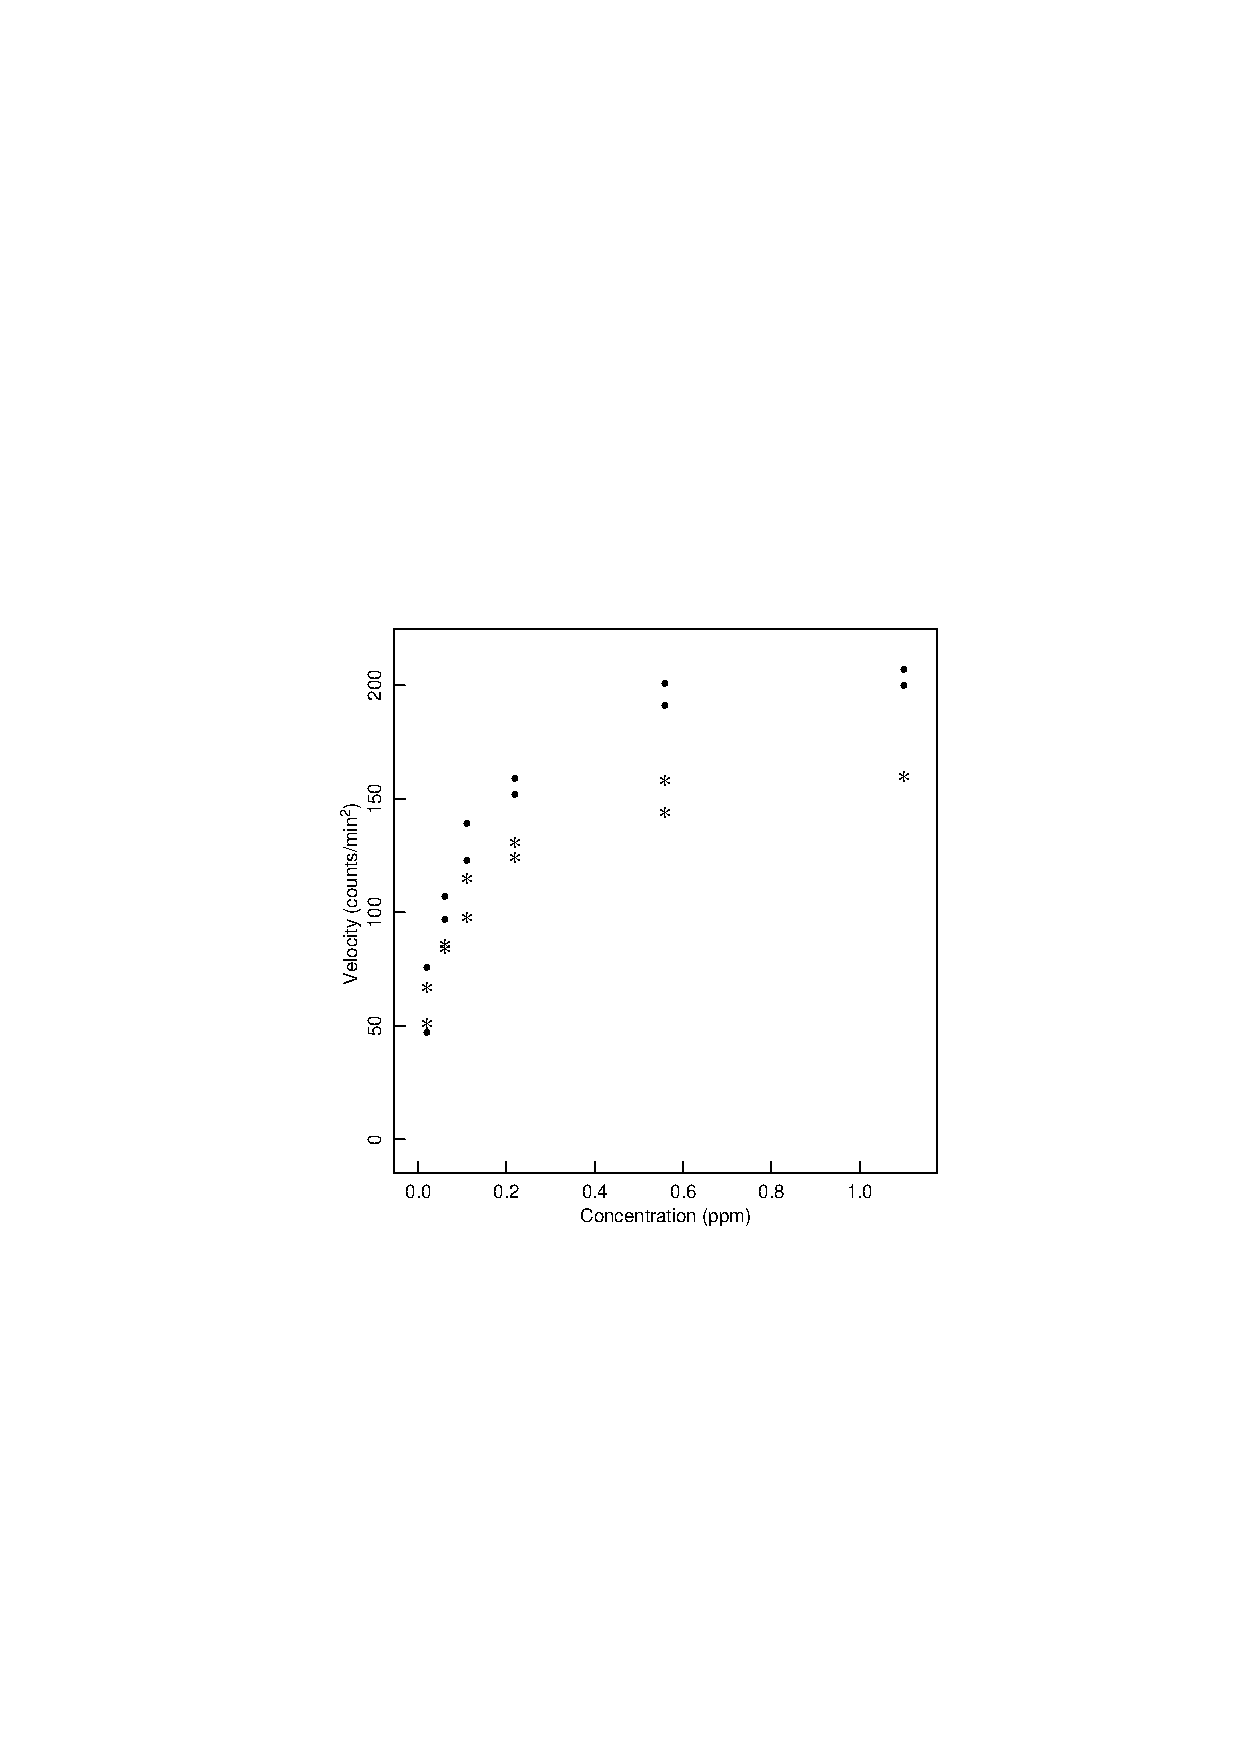
\includegraphics{3MIC2data}}%,height=3in}}
    \caption{Plot of enzyme velocity data versus substrate concentration.
      The data for the enzyme treated (not treated) with Puromycin are
      shown as ().}
    \label{fig:MIC2data}
  \end{figure}
  
  To determine if the $\theta_{2}$ parameter is unchanged,
  we use an extra sum of squares analysis, which requires fitting a full and a
  partial model.
  The full model corresponds to completely different sets of
  parameters for the treated data and the untreated data, while
  the partial model corresponds to different $\theta_{1}$
  parameters but the same $\theta_{2}$ parameter.
  To combine the full and partial models, we introduce
  the \emph{indicator variable}
  \begin{displaymath}
    x_2 = \left\{ 
      \begin{array}{ll}
        0 & \mbox{\rm untreated}\\
        1 & \mbox{\rm treated}
      \end{array}
    \right.
  \end{displaymath}
  
  and let $x_1$ be the substrate concentration.
  The combined model is then written
  \begin{displaymath}\label{eqn:combin}
    f(\bx,\btheta)=\frac{(\theta_1 + \phi_1 x_2 ) x_1}{(\theta_2+\phi_2 x_2)+x_1}
  \end{displaymath}
  where
  $\theta_{1}$ is the maximum velocity for the untreated enzyme,
  $\phi_{1}$ is the incremental maximum velocity due to the
  treatment,
  $\theta_{2}$ is the (possibly common) ``half-velocity''
  point, and $\phi_{2}$ is the change in the half-velocity due to the
  treatment.
  Since we expect $\phi_{1}$ to be nonzero, we are interested
  in testing whether $\phi_{2}$ could be zero.
  
  The model (\ref{eqn:combin}) was fitted and the results of this fit are
  shown in Table~\ref{tbl:treloar3}.
  \begin{table}
    \caption{
      Parameter summary for the 4-parameter Michaelis--Menten model fitted
      to the combined Puromycin data set.
    }\label{tbl:treloar3}
    \begin{center}
      \begin{tabular}{cccccccc} \hline
        & &\multicolumn{1}{c}{Approx.}&&\multicolumn{4}{c}{Correlation}\\
        \multicolumn{1}{c}{Parameter} &\multicolumn{1}{c}{Estimate}& \multicolumn{1}{c}{Std. Err.}&\multicolumn{1}{c}{$t$ Ratio} &\multicolumn{4}{c}{Matrix}\\ \hline
        $\theta_{1}$ &160.3 & 6.90 & 23.2 &1.00\\
        $\theta_{2}$ & 0.0477 & 0.00828 & 5.8 & 0.77 & 1.00\\
        $\phi_{1}$ & 52.4 & 9.55 & 5.5 &--\/0.72 & --\/0.56 & 1.00\\
        $\phi_{2}$ & 0.0164 & 0.0114 &1.4 &--\/0.56 & --\/0.72 & 0.77 & 1.00\\ \hline
      \end{tabular}
    \end{center}
  \end{table}
  It appears that $\phi_{2}$ could be zero, since it has a small
  $t$ ratio, and so we fit the
  partial model (\ref{eqn:combin}) with $\phi_2 = 0$.
  The results of this fit are given in
  Table~\ref{tbl:treloar4} and
  \begin{table}
    \caption{
      Parameter summary for the 3-parameter Michaelis--Menten model fitted
      to the combined Puromycin data set.
    }\label{tbl:treloar4}
    \begin{center}
      \begin{tabular}{ccccccc}\hline
        & & \multicolumn{1}{c}{Approx.}&&\multicolumn{3}{c}{Correlation}\\
        \multicolumn{1}{c}{Parameter} &\multicolumn{1}{c}{Estimate}& \multicolumn{1}{c}{Std. Err.} &\multicolumn{1}{c}{$t$ Ratio} & \multicolumn{3}{c}{Matrix}\\ \hline
        $\theta_{1}$&166.6&5.81&28.7&1.00\\
        $\theta_{2}$&0.058&0.00591&9.8&0.61&1.00\\
        $\phi_{1}$&42.0&6.27&6.7&--\/0.54&0.06&1.00\\ \hline
      \end{tabular}
    \end{center}
  \end{table}
  the extra sum of squares analysis is presented in
  Table~\ref{tbl:treloar}.
  \begin{table}
    \caption{
      Extra sum of squares analysis for the 3- and 4-parameter
      Michaelis--Menten model fitted to the combined Puromycin data set.
    }\label{tbl&treloar}
    \begin{center}
      \begin{tabular}{cccccc}\hline
        & \multicolumn{1}{c}{Sum of} & \multicolumn{1}{c}{Degrees of}
        &\multicolumn{1}{c}{Mean}\\ \multicolumn{1}{c}{Source} &
        \multicolumn{1}{c}{Squares} &\multicolumn{1}{c}{Freedom} &
        \multicolumn{1}{c}{Square} & \multicolumn{1}{c}{F Ratio}
        &\multicolumn{1}{c}{$p$ Value}\\
        \hline Extra&186&1&186.&1.7&0.21\\
        4-parameter&2055&19&108.2\\
        3-parameter&2241&20\\ \hline
      \end{tabular}
    \end{center}
  \end{table}
  
  In this well-designed experiment, which includes replications, it
  is also possible to analyze for lack of fit of the partial model as
  shown in Table~\ref{tbl:treloar5}.
  \begin{table}
    \caption{
      Lack of fit analysis for the 3-parameter Michaelis--Menten model
      fitted to the combined Puromycin data set.  }\label{tbl&treloar5}
    \begin{center}
      \begin{tabular}{cccccc}
        & \multicolumn{1}{c}{Sum of} & \multicolumn{1}{c}{Degrees
          of} & \multicolumn{1}{c}{Mean}\\ \multicolumn{1}{c}{Source} &
        \multicolumn{1}{c}{Squares} & \multicolumn{1}{c}{Freedom} &
        \multicolumn{1}{c}{Square} & \multicolumn{1}{c}{F Ratio} &
        \multicolumn{1}{c}{$p$ Value}\\ \hline
        Lack of fit &1144&9&127.3&1.3&0.35\\
        Replication&1097&11&99.7\\ \hline
        Residuals&2241&20\\ \hline
      \end{tabular}
    \end{center}
  \end{table}
  These summary calculations, together with plots of the residuals
  (not shown), suggest that a model which has a common
  half-velocity parameter and a higher asymptotic velocity for
  the treated enzyme is adequate.
\end{example}

In the above example, the $t$ ratios for the
incremental parameters permit reliable
inferences to be made concerning changes from one block to
another.
We recommend, however, that the extra sum of squares analysis
always be used,
since it is unaffected by parameter effects
nonlinearity (see Chapter 7) and is therefore more exact than the $t$ test
in the nonlinear case.
We only use the $t$ ratios to suggest which incremental
parameters might be zero and should be investigated
further:
the actual decision on whether to retain a parameter should be based on an
extra sum of squares analysis or a profile $t$ analysis (see Chapter 6).

In summary, incremental parameters provide a direct and simple
procedure for determining whether changes in parameters occur
between different blocks.
Clearly, incremental parameters can also be used
to advantage in linear least squares to
determine changes in parameters between blocks, since then the
$t$ tests are exact.
Even for linear least squares, however, we recommend fitting the
reduced model and using the extra sum of squares analysis to
make any final decisions concerning inclusion or deletion of
parameters, so as to avoid problems with multicollinearity and inflation
of variances.
Incremental parameters can also be used when there are more than
two blocks by introducing additional indicator variables or,
possibly, by rewriting the parameters as functions of other
variables as in Section 3.11.

\subsection{Non-nested Models}

When trying to decide which of several \emph{non-nested} models is
best, the first approach should be to the researcher.
That is, if there are scientific reasons for preferring one model
over the others, strong weight should be given to the
researcher's reasons because the primary aim of data analysis is
to explain or account for the behavior of the data, not simply to
get the best fit.

If the researcher cannot provide convincing reasons for choosing
one model over others, then statistical analyses can be used, the
most important of which is probably an analysis of the residuals.
Generally the model with the smallest residual mean square and
the most random-looking residuals should be chosen.
The residuals should be plotted versus the predicted values, the
control variables, time order, and any other (possibly lurking)
variables; see Section 3.7.

\section{Parameters as Functions of Other Variables}
\index{practical considerations!parameters as functions of other variables}
\index{parameter!as functions of other variables}

In many situations, the parameters in a mechanistic model will
depend on other variables.
For example, in chemical kinetic studies, we may have data from
several experiments in which the operating conditions have been
varied, and it may be thought that the rate constants should depend in
some systematic way on the operating conditions.
We would then like to fit a model which
incorporates the dependence of the \emph{kinetic parameters}
$\btheta$ on some \emph{process variables}, say $\bw$, and some
\emph{process parameters},
\index{parameter!process}
$\bphi = ( \phi_1 ,\ldots, \phi_L ) \trans$.
That is, $\btheta = \btheta ( \bw , \bphi )$.
The expectation function is then
$f ( \bx , \btheta ) = f ( \bx , \btheta ( \bw , \bphi ) )$.

To estimate the parameters in such an extended model, we could express
the function in terms of the regular variables $\bx$, the process
variables $\bw$, and the process parameters $\bphi$, determine the
derivatives with respect to $\bphi$, and then use a Gauss--Newton
algorithm to converge to $\hat{\bphi}$.
It is more efficient, however, to build on what we already have
and proceed as follows:
\begin{enumerate}
\item At each level of $\bw$, estimate the kinetic parameters
  $\btheta$ in the regular model.
\item Plot the parameter estimates $\hat \theta_{p}$ versus $\bw$
  to determine a plausible form for the relationship of $\hat
  \theta_{p}$ to $\bw$ and to obtain starting estimates for
  the process parameters $\bphi$.
\item  Use the chain rule for derivatives to determine the
  derivatives with respect to $\bphi$, exploiting the existing
  derivatives with respect to $\btheta$, as
  \begin{displaymath}
    \frac{\partial\eta_n}{\partial\phi_l}=\sum_{p=1}^P
    \frac{\partial\eta_n}{\partial\theta_p} 
    \frac{\partial\theta_p}{\partial\phi_l}
  \end{displaymath}
  for $l= 1 ,2 ,\ldots, L$, where $L$ is the total number of
  process parameters.
\end{enumerate}
An application of this method is described in Section 5.5.

\begin{example}\label{mic:pfunc}

  Suppose in the research on Puromycin (Example Puromycin \ref{mic:10})
  there were, say, four treatment levels of Puromycin instead of
  just two (treated and untreated).
  We could then proceed by incorporating three indicator variables to
  account for changes in the parameters due to different
  treatments.
  However, if the Puromycin treatments consist of different doses,
  it might be possible to write
  \begin{displaymath}
    f ( x , \btheta ) = \frac{\theta_1(w)x}{\theta_2(w)+x}
  \end{displaymath}
  where a possible form of $\theta_{1}$ and $\theta_{2}$ is
  \begin{eqnarray*}
    \theta_1&=&\phi_{10} + \phi_{11}  w\\
    \theta_2&=&\phi_{20} + \phi_{21}  w
  \end{eqnarray*}
  In this example, the (regular) variable is $x$, the substrate
  concentration, and the process variable is $w$, the Puromycin
  concentration.
  
  Now suppose that at Puromycin concentration $w_{1}$ we get
  estimates
  $\hat \theta_{11}$ and $\hat \theta_{21}$, at concentration
  $w_{2}$, we get estimates $\hat \theta_{12}$ and $\hat \theta_{22}$,
  and so on, and that a plot of $\hat \theta_{2}$ versus $w$ looks
  essentially flat, which suggests
  $\theta_2 =\mbox{\rm constant}$.
  Then we would choose $\phi_{20} = \hat \theta_{2}$.
  Suppose further that the plot of $\hat \theta_{1}$ versus $w$
  reveals a straight line relationship,
  $\theta_1 = \phi_{10} + \phi_{11} w$.
  We could then use linear regression of $\hat \theta_{1}$ on $w$
  to get starting estimates for $\phi_{10}$ and $\phi_{11}$.
  
  The model to be fitted to the combined data vector would be
  \begin{eqnarray*}
    f(x,w,\bphi)&=&\frac{\theta_1(w)x}{\theta_2(w)+x}\\
    &=&\frac{(\phi_{10}+\phi_{11}w)x}{\phi_{20}+x}
  \end{eqnarray*}
\end{example}

\section{Presenting the Results}
\index{practical considerations!presenting the results}
\index{report!writing}

As in all statistical analyses,
the results from a nonlinear regression analysis should be
presented clearly and succinctly.
This is usually done most effectively by considering the needs
and abilities of the prospective audience.
The report should always include a summary of the main findings
and conclusions.

The summary should include a
statement of the final model, the parameter estimates and their
standard errors, and an interpretation of the model and the
parameters in the context of the original problem.

In the main body of the report, it is useful to state the
original problem and possibly a derivation of the general form of
mechanistic model proposed.
Plots of the data should be given, and any preliminary analyses
should be discussed, particularly if they involved transformation
of the data or the expectation function.
A listing of the data should always be included (perhaps in an
appendix), but otherwise plots should be used for effective
communication.

The initial model should be presented with a brief
description of the steps taken to reduce or extend it, if
necessary referring to detailed analyses in appendices.
The final model, together with parameter estimates and their
approximate standard errors and correlation matrix should be
stated, along with a plot of the data, the fitted expectation
function, and an approximate confidence band for the
expectation function.
Pairwise plots of the parameter inference region,
and possibly profile $t$ plots,
as described in Chapter 6, should be given.
Of great importance is an interpretation of the expectation
function and the parameter values relative to the original
problem, and especially any new findings, such as the need for
additional variables in the model or the non-necessity of any
variables or parameters.

Finally, conclusions and recommendations should be made,
especially concerning possible future experiments or development
of the research.

For further tips on report writing, see \citeasnoun{ehre:1981},
%\glossary{ Ehrenberg, A.S.C.}
\citeasnoun{ehre:1982}, and \citeasnoun{watt:1981}.
%\glossary{ Watts, D.G.}
The preparation and presentation of graphical material is covered in
\citeasnoun{tuft:1983}, \citeasnoun{clev:1984},
\citeasnoun{clev:1985}, and \citeasnoun{cham:clev:klei:tuke:1983}.
%\glossary{ Tufte, E.R.}
%\glossary{ Cleveland, W.S.}
%\glossary{ Chambers, J.M.}
%\glossary{ Kleiner, B.}
%\glossary{ Tukey, P.W.}

\section{Nitrite Utilization:  A Case Study}

To illustrate the techniques presented in this chapter, we present an
analysis of data on the utilization of nitrite in bush beans as
a function of light intensity \cite{elli:peir:1986}.
%\glossary{ Elliott, J.R.}
%\glossary{ Peirson, D.R.}
Portions of primary leaves from three
16-day-old bean plants were subjected to eight levels of light
intensity ($\mu$E/m$^{2}$s), and the nitrite utilization
(nmol/ghr) was measured.
The experiment was repeated on a different day, resulting in the
data listed in Appendix~\ref{atbl:nitrite}.

The experimenters did not have a theoretical mechanism to explain
the behavior, but they thought that nitrite utilization should be
zero at zero light intensity, and should tend to an asymptote as
light intensity increased.
\subsection{Preliminary Analysis}
\index{preliminary analysis!nitrite example}

From a plot of the data
\begin{figure}
  \centerline{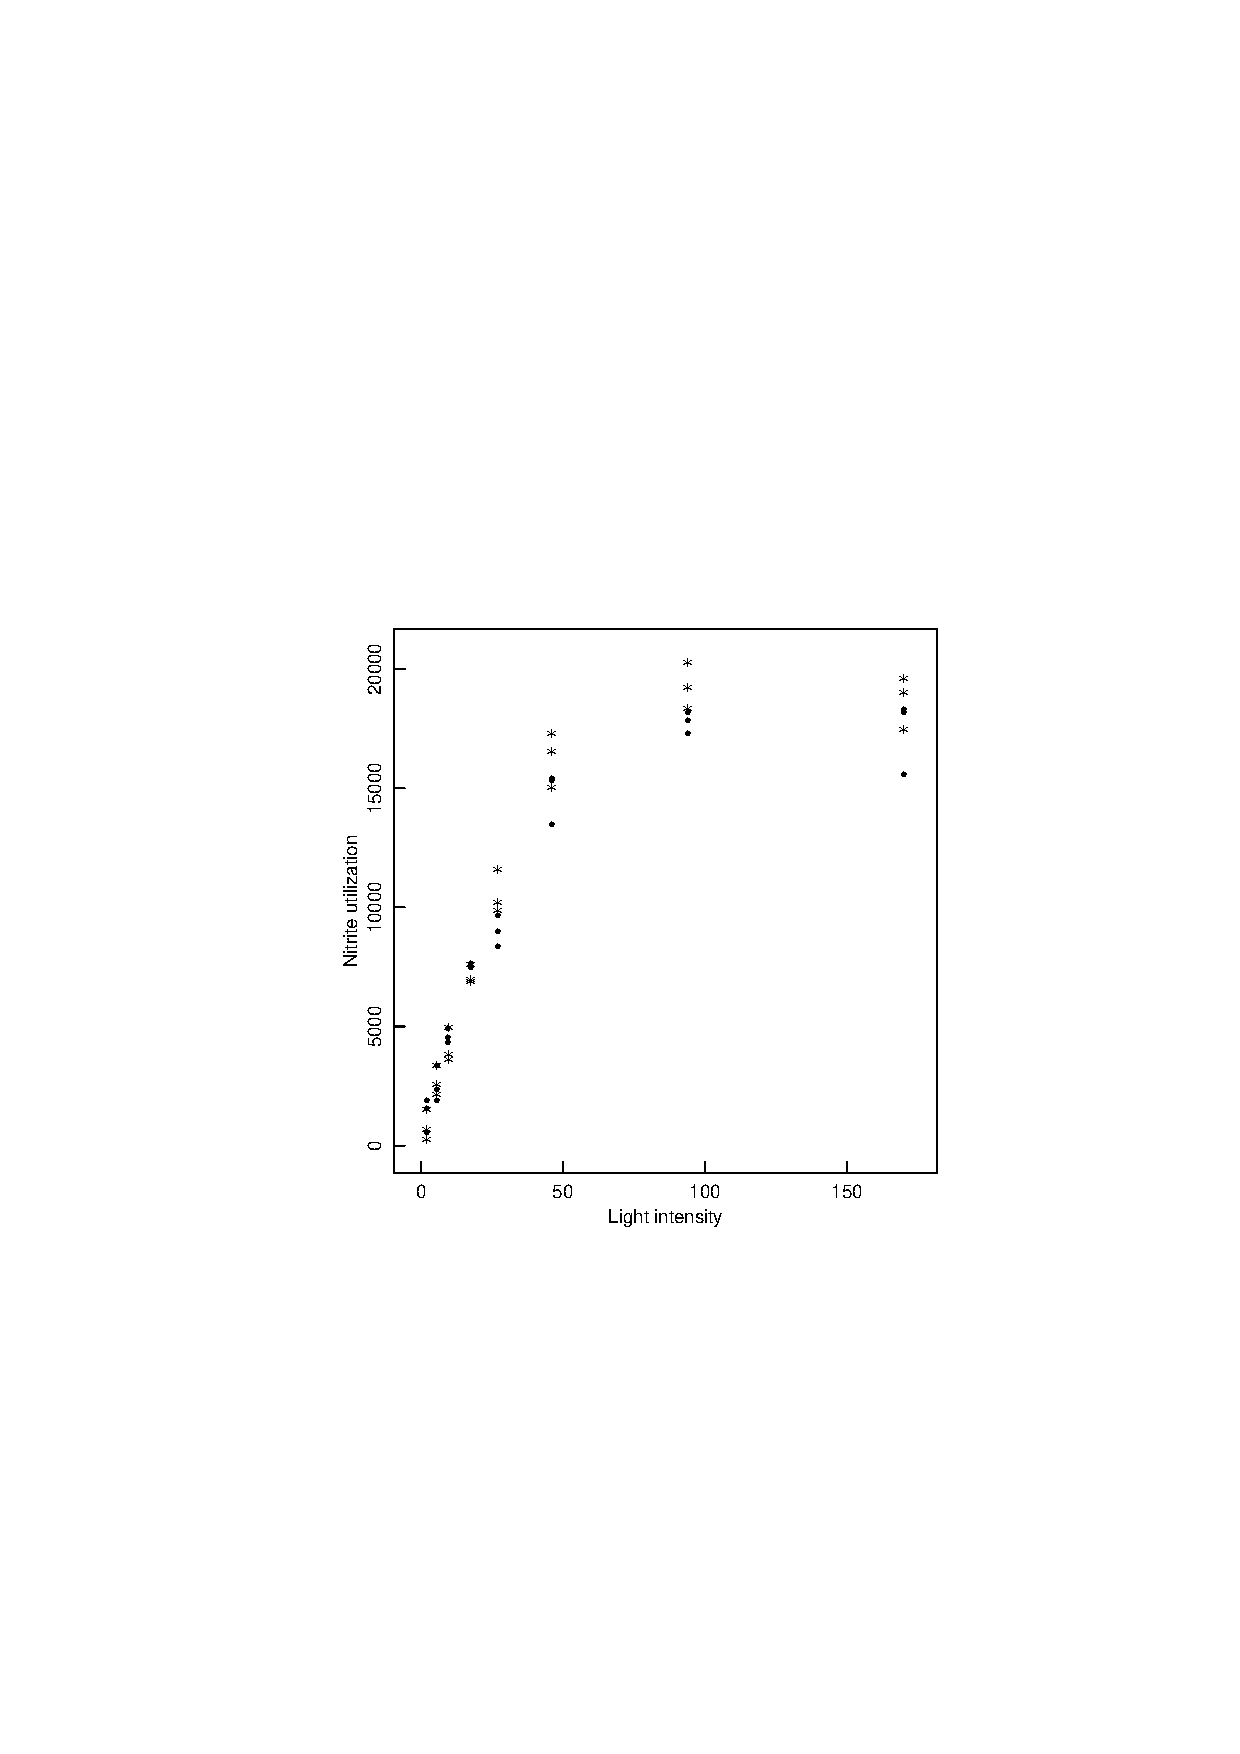
\includegraphics{3NITdata}}%,height=3in}}
  \caption{Plot of nitrite utilization by bean plants
    versus light intensity for day 1 (*) and day 2 ().}
  \label{fig:NITdata}
\end{figure}
(Figure~\ref{fig:NITdata}) it can be seen that there
was a difference in the nitrite utilization
between experiments on the two days,
particularly at higher light intensities.
There is also a tendency for the response to drop at high light
intensity.
Note too that, even though the response ranges from 200 to 20000
nmol/ghr, the variance is effectively constant;  there is no
need to transform to stabilize variance.
To verify the apparent stable variance, we performed a two way
analysis of variance using indicator variables for days and for
\index{analysis of variance!nitrite example}
\index{indicator variable!nitrite example}
light intensities, with the results shown in
Tables~\ref{tbl:3.2} and \ref{tbl:3.3}.
\begin{table}
  \caption{
  Two way analysis of variance for the nitrite utilization data.
  }\label{tbl:3.2}
  \begin{center}
    \begin{tabular}{cccccc}\hline
      &\multicolumn{1}{c}{Sum of} & \multicolumn{1}{c}{Degrees}
      &\multicolumn{1}{c}{Mean}\\ & \multicolumn{1}{c}{Squares} &
      \multicolumn{1}{c}{of} &\multicolumn{1}{c}{Square}\\
      \multicolumn{1}{c}{Source} & \multicolumn{1}{c}{$( 10^6 )$} &
      \multicolumn{1}{c}{Freedom} & \multicolumn{1}{c}{$( 10^6 )$} &
      \multicolumn{1}{c}{F Ratio} & \multicolumn{1}{c}{$p$ Value}\\ \hline
      Days&4.23&1&4.23&6.1&0.02\\
      Intensity&2040&7&291.5&420.&0.00\\
      Days$\times$intensity&10.07&7&1.44&2.1&0.08\\ \hline
      Replication&22.21&32&0.694\\ \hline
    \end{tabular}
  \end{center}
\end{table}
\begin{table}
  \caption{
  Replication averages and standard deviations for the nitrite
  utilization data.}\label{tbl:3.3}
  \begin{center}
    \begin{tabular}{ccccc}\hline
      &\multicolumn{2}{c}{Day 1} & \multicolumn{2}{c}{Day 2}\\ \hline
      && \multicolumn{1}{c}{Standard} && \multicolumn{1}{c}{Standard}\\
      \multicolumn{1}{c}{Intensity}
      &\multicolumn{1}{c}{Average}&\multicolumn{1}{c}{Deviation} &
      \multicolumn{1}{c}{Average} & \multicolumn{1}{c}{Deviation}\\ \hline
      2.2&826&652&1327&694\\
      5.5&2702&623&2541&758\\
      9.6&4136&719&4619&296\\
      17.5&7175&401&7554&86\\
      27.0&10567&908&9019&650\\
      46.0&16302&1154&14753&1082\\
      94.0&19296&963&17786&430\\
      170.0&18719&1117&17374&1408\\ \hline
    \end{tabular}
  \end{center}
\end{table}
For our purposes the most useful information from the two way analysis
of variance is the replication sum of squares and mean square,
which can be used for testing lack of fit.
We note, however, that the lack of a significant
day$\times$intensity interaction suggests that some of the model parameters
may be equal for the two days, although the
significant day effect tends to corroborate the observed
difference between the heights of the maxima on the two days.
A plot of the replication
\begin{figure}
  \centerline{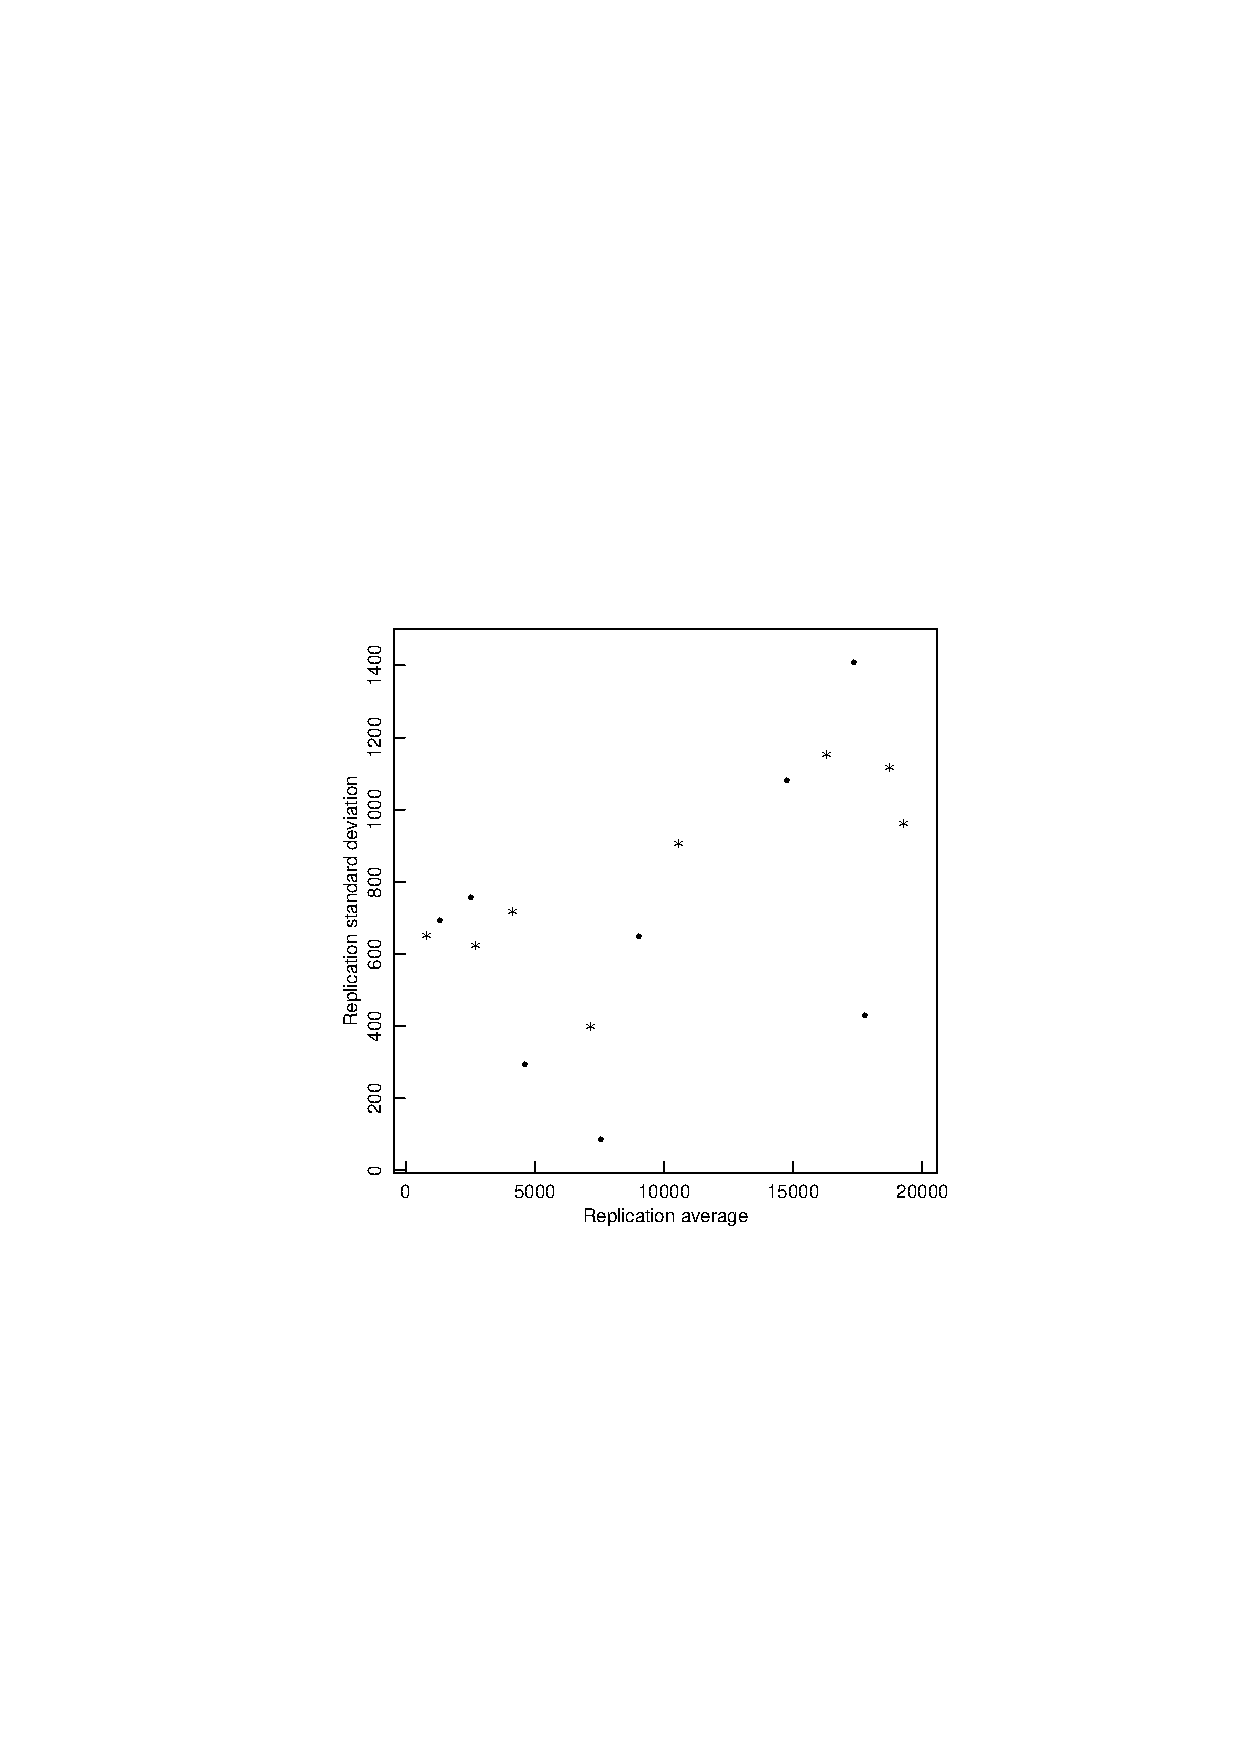
\includegraphics{3NITrep}}%,height=2.75in}}
  \caption{Replication standard deviations plotted versus replication
    averages for the nitrite utilization data.  Day 1 data are shown
    as $*$ and day 2 data as .}
  \label{fig:NITrep}
\end{figure}
standard deviations versus the replication averages, shown in
Figure~\ref{fig:NITrep}, verified our earlier assessment that the
variance is stable since there is no systematic relation,
and so we proceed to model fitting.

Note that the analysis of variance is used here only as a screening
tool.
It is not intended as a final analysis of these data, since the
underlying additive linear model assumed in an analysis of variance is
not appropriate.

\subsection{Model Selection}
\index{model!selection, nitrite example}

Because the researchers did not have a model in mind, it was
necessary to select one on the basis of the behavior of the data.
The Michaelis--Menten model
\begin{displaymath}
  f(x,\btheta)=\frac{\theta_1x}{\theta_2+x}
\end{displaymath}
and the simple exponential rise model
\begin{displaymath}
f (x , \btheta ) = \theta_1 ( 1 - e^{ - \theta_2 x } )
\end{displaymath}
were selected because they met the researcher's beliefs
that nitrite utilization was zero at zero light intensity and tended to
an asymptote as the light intensity increased.
To simplify the description, we give details for the
Michaelis--Menten model analysis, and only present summaries for
the exponential rise model.

Since there are 24 observations for each day from this
well-designed experiment, it would be reasonable to fit a
separate model for each day.
We would like to think, however, that the same
parameter values, or at least some of the same
parameter values, would be valid for both days, and so
we proceed to fit a model for day 1 with incremental
parameters for day 2.
\index{incremental parameter!nitrite example}
That is, we write
\begin{displaymath}
f(x,\btheta)=\frac{(\theta_1+\phi_1x_2)x_1}{(\theta_2+\phi_2 x_2)+x_1}
\end{displaymath}
where $x_{1}$ is the light intensity and $x_{2}$ is an
indicator variable
\begin{displaymath}
x_2 = \left\{
  \begin{array}{l l}
    0&\mbox{\rm day 1}\\
    1&\mbox{\rm day 2}
  \end{array}\right.
\end{displaymath}
as described in Section 3.10.

\subsection{Starting Values}

Since the maximum value on day 1 is about 20,000, and on day 2 is
about 18,000, we choose $\theta_1^0=25000$ and
$\phi_1^0=-3000$.
The response reaches about 12500 at a light intensity of about 34
for day 1 and 35 for day 2, which gives $\theta_2^0=34$ and
$phi_2^0=1$.

\subsection{Assessing the Fit}
\index{assessing fit!nitrite example}

Convergence was achieved at the values shown in
Table~\ref{tbl:3.4}.
\begin{table}
  \caption{
  Parameter summary for the 4-parameter Michaelis--Menten model
  fitted to the nitrite utilization data.
  }\label{tbl:3.4}
  \begin{center}
    \begin{tabular}{cccccccc}\hline
      &&\multicolumn{1}{c}{Standard}&&\multicolumn{4}{c}{Correlation}\\
      \multicolumn{1}{c}{Parameter}&\multicolumn{1}{c}{Estimate}&
      \multicolumn{1}{c}{Error}&\multicolumn{1}{c}{$t$ Ratio} &
      \multicolumn{4}{c}{Matrix}\\ \hline
      $\theta_{1}$&24743&1241&19.9&1.00\\
      $\theta_{2}$&35.27&4.66&7.6&0.88&1.00\\
      $\phi_{1}$&--2329&1720&--1.4&--\/0.72&--\/0.64&1.00\\
      $\phi_{2}$&--2.174&6.63&--\/0.3&--\/0.62&--\/0.70&0.88&1.00\\ \hline
    \end{tabular}
  \end{center}
\end{table}
It appears from the $t$ ratios that both the
incremental parameters could be estimates of zero, and so a
common model could be fitted.
However, if we do a lack of fit analysis on this model as in
\index{lack of fit!analysis, nitrite example}
Table~\ref{tbl:mic4lof},
we see that this four-parameter model is not adequate.
\begin{table}
  \caption{
  Lack of fit analysis for the 4-parameter Michaelis--Menten model
  fitted to the nitrite utilization data.}\label{tbl:mic4lof}
  \begin{center}
    \begin{tabular}{lccccc}\hline
      &\multicolumn{1}{c}{Sum of} &\multicolumn{1}{c}{Degrees}
      &\multicolumn{1}{c}{Mean}\\ & 
      \multicolumn{1}{c}{Squares}& \multicolumn{1}{c}{of}
      &\multicolumn{1}{c}{Square}\\ 
      Source&\multicolumn{1}{c}{$(10^6 )$}&\multicolumn{1}{c}{Freedom}
      &\multicolumn{1}{c}{$(10^6 )$} &\multicolumn{1}{c}{F Ratio}&
      \multicolumn{1}{c}{$p$ Value}\\ \hline
      Lack of fit&64.30&12&5.36&7.72&0.00\\
      Replications&22.21&32&0.694\\ \hline
      Residuals&86.51&44\\ \hline
    \end{tabular}
  \end{center}
\end{table}
(The same conclusion was reached for the exponential rise model,
in this case with a lack of fit ratio of 3.2,
corresponding to a $p$ value of 0.00.)

A plot of the residuals versus light intensity,
as in
\begin{figure}
  \centerline{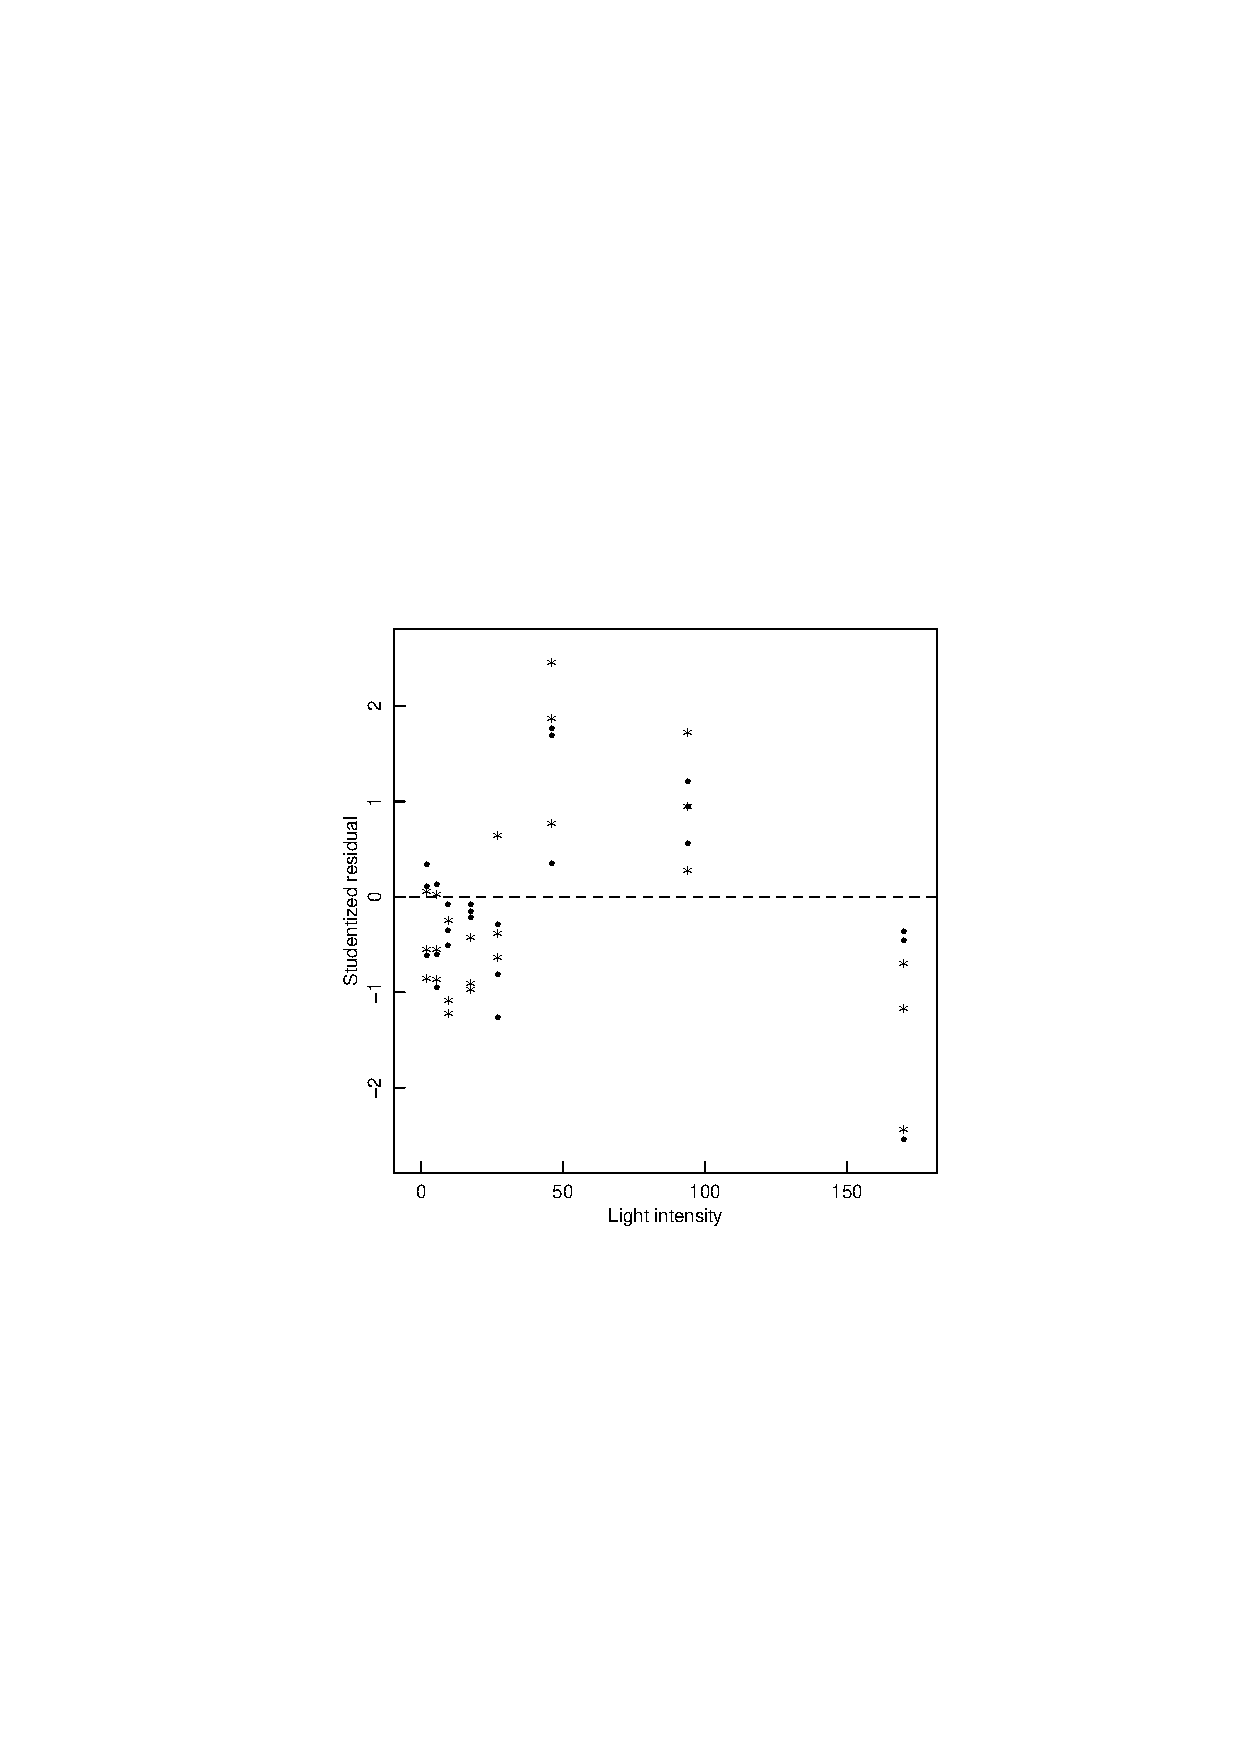
\includegraphics{3NITres1}}%,height=3in}}
  \caption{Studentized residuals from the 4-parameter
    Michaelis--Menten model plotted versus light intensity.  Day 1
    data are shown as $*$ and day 2 data as .}
\label{fig:NITres1}
\end{figure}
Figure~\ref{fig:NITres1}, reveals nonrandom
behavior, with negative residuals at small and large intensities
and positive ones in the middle.
The model must therefore be modified to allow the nitrite
utilization to drop with increasing light intensity, rather than
leveling off as suggested by the researchers.

\subsection{Modifying the Model}

To alter the Michaelis--Menten expectation function to rise to a
peak and then fall, we added a quadratic term to the denominator to
produce the quadratic Michaelis--Menten model,
\begin{displaymath}
  f(x,\btheta)=\frac{\theta_1x}{\theta_2+x+\theta_3x^2}
\end{displaymath}
which, with incremental parameters and an indicator variable
for the different days, becomes
\begin{displaymath}
  f(\bx,\btheta)=\frac{(\theta_1+\phi_1 x_2)x_1}{(\theta_2+\phi_2x_2)+x_1
    +(\theta_3+\phi_3x_2)x_1^2}
\end{displaymath}
(For the exponential rise model, we replaced the unit term by an
exponential to produce the exponential difference model,
\begin{displaymath}
f = \theta_1 ( e^{ - \theta_3 x } -
e^{ - \theta_2 x } )
\end{displaymath}
This model, augmented with increment parameters and an
indicator variable, was also used to fit the data.)

Starting values for the parameters were obtained by taking
reciprocals of the function and the data and using linear least
squares for the quadratic Michaelis--Menten model.
Taking reciprocals worked for the day 2 data, giving
$\btheta=(107411,234,0.024)\trans$, but gave some
negative values for the day 1 data.
We therefore used the day 2 starting values with slight
perturbations to get starting values for the 6-parameter model of
$\btheta^0=( 110000 ,234 ,0.024 ) \trans$ and
$\bphi^0=( -10000 ,23 ,0.002 ) \trans$.
(For the exponential difference model, we guessed that the two
rate constants might be in the ratio 1:5 and used the estimate
for $\theta_{2}$ to give $\theta_3 =0.006$.
We then estimated $\theta_{1}$ by evaluating
\begin{displaymath}
  \theta_1=\frac{y}{e^{{-0.006x}}-e^{{-0.030x}}}
\end{displaymath}
for several $x$ values.  This gave $\theta_1^{0}=37000$
for the day 1 data and $35000$ for the day 2 data, from which we
got $\phi_1^0 = -2000$.)

\subsection{Assessing the Fit}
\index{assessing fit!nitrite example}

Quick convergence was achieved
to the parameter estimates given in
Table~\ref{tbl:3.5} for the quadratic Michaelis--Menten model.
\begin{table}
  \caption{
  Parameter summary for the 6-parameter quadratic Michaelis--Menten model
  fitted to the nitrite utilization data.}\label{tbl:3.5}
  \begin{center}
    \begin{tabular}{ccccccccc}\hline
      &&\multicolumn{1}{c}{Standard}&&\multicolumn{5}{c}{Correlation}\\
      \multicolumn{1}{c}{Parameter}&\multicolumn{1}{c}{Estimate}&
      \multicolumn{1}{c}{Error}& \multicolumn{1}{c}{$t$ Ratio} &
      \multicolumn{5}{c}{Matrix}\\ \hline
      $\theta_{1}$&89846&37583&2.4&1.00\\
      $\theta_{2}$&186.7&90.1&2.1&1.00&1.00\\
      $\theta_{3}$&0.01626&0.00922&1.8&1.00&0.99&1.00\\
      $\phi_{1}$&--38956&40020&--1.0&--\/0.94&--\/0.94&--\/0.94&1.00\\
      $\phi_{2}$&--83.23&96.8&--\/0.9&--\/0.93&--\/0.93&--\/0.92&1.00&1.00\\
      $\phi_{3}$&--\/0.00846&0.0993&--\/0.9&--\/0.93&--\/0.92&--\/0.93&1.00&0.99\\ \hline
    \end{tabular}
  \end{center}
\end{table}
All the incremental parameters have nonsignificant approximate
$t$ ratios, which suggests that the parameters could be zero, and
so a simpler model may be adequate.
The extremely high parameter approximate correlations also lead one to
suspect that the model may be overparametrized.
\index{overparametrization!nitrite example}
The residual sum of squares ($32.02 \times 10^{6}$ on 42 df)
is only about a third of that for the previous model.
(Similar conclusions were reached for the 6-parameter exponential
difference model.)

The residuals for this model, plotted versus light intensity in
\begin{figure}
  \centerline{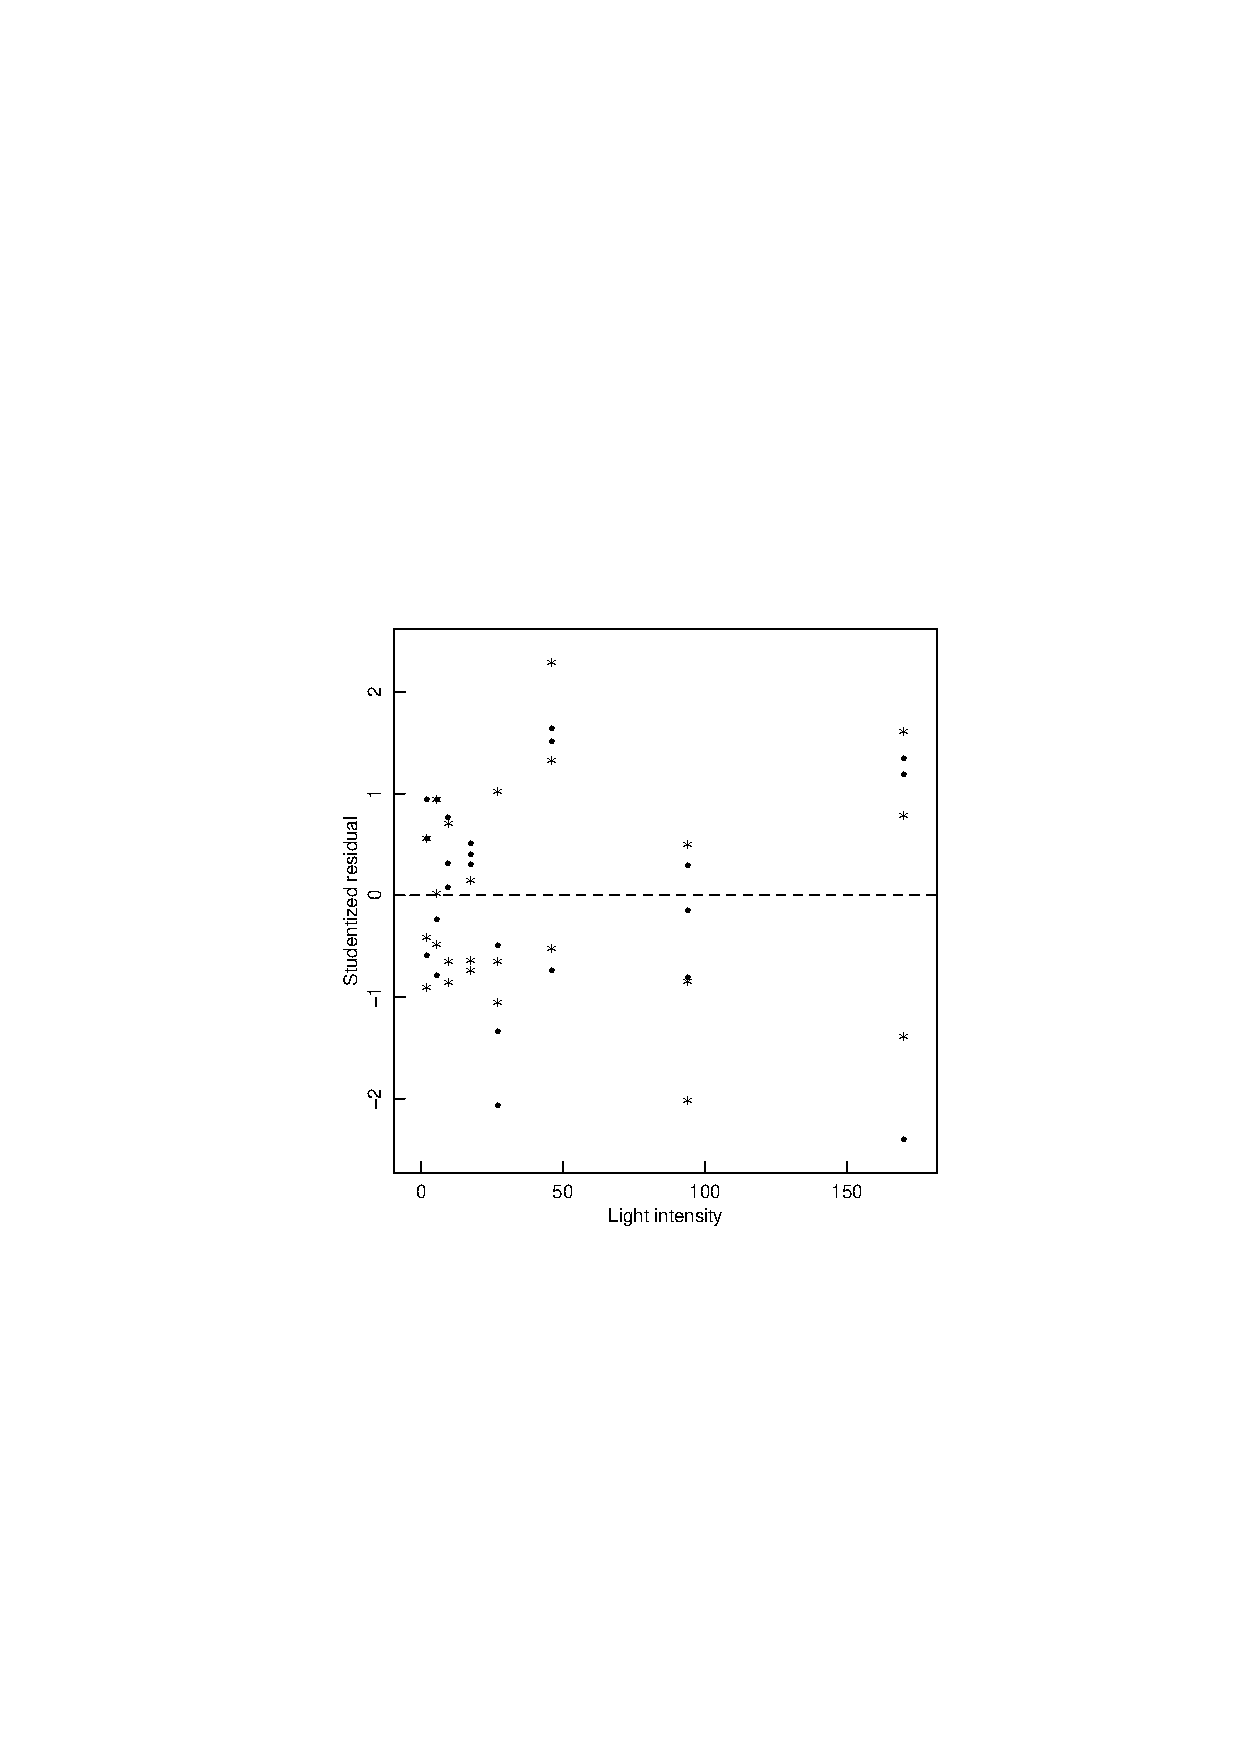
\includegraphics{3NITres2}}%,height=3in}}
  \caption{Studentized residuals from the 6-parameter quadratic
    Michaelis--Menten model plotted versus light intensity.  Day 1
    data are shown as * and day 2 data as $\cdot$.}
  \label{fig:NITres2}
\end{figure}
Figure~\ref{fig:NITres2}, are clearly well behaved and give no
evidence of inadequacy of the model.

\subsection{Reducing the Model}

To determine what simplifications could be made in the quadratic
Michaelis--Menten model,
we set $\phi_{2}$ and $\phi_{3}$ to zero,
still retaining $\phi_{1}$
to account for a difference between days.
For starting values, we simply used the relevant converged values
from the 6-parameter model.

\subsection{Assessing the Fit}
\index{assessing fit!nitrite example}

The results for the 4-parameter quadratic model are given in
Table~\ref{tbl:3.6}.
\begin{table}
  \caption{
  Parameter summary for the 4-parameter quadratic Michaelis--Menten model
  fitted to the nitrite utilization data.}\label{tbl:3.6}
  \begin{center}
    \begin{tabular}{cccccccc}\hline
      &&\multicolumn{1}{c}{Standard} &&\multicolumn{4}{c}{Correlation}\\
      Parameter & \multicolumn{1}{c}{Estimate}&
      \multicolumn{1}{c}{Error} &\multicolumn{1}{c}{$t$ Ratio} &
      \multicolumn{4}{c}{Matrix}\\ \hline 
      $\theta_{1}$&70096&16443&4.3&1.00\\
      $\theta_{2}$&139.4&39.3&3.6&1.00&1.00\\
      $\theta_{3}$&0.01144&0.00404&2.8&0.99&0.99&1.00\\
      $\phi_{1}$&--5381&1915&--2.8&--\/0.69&--\/0.66&--\/0.66&1.00\\ \hline
    \end{tabular}
  \end{center}
\end{table}
The extra sum of squares analysis for the 4-parameter
\index{extra sum of squares!nitrite example}
versus the 6-parameter quadratic model, shown in
Table~\ref{tbl:3.7},
\begin{table}
  \caption{
  Extra sum of squares analysis for the 6-parameter
  versus the 4-parameter quadratic Michaelis--Menten model
  fitted to the nitrite utilization data.
  }\label{tbl:3.7}
  \begin{center}
    \begin{tabular}{cccccc}\hline
      &\multicolumn{1}{c}{Sum of}&\multicolumn{1}{c}{Degrees}&
      \multicolumn{1}{c}{Mean}\\
      &\multicolumn{1}{c}{Squares} &\multicolumn{1}{c}{of}
      &\multicolumn{1}{c}{Square}\\ 
      \multicolumn{1}{c}{Source}&\multicolumn{1}{c}{$( 10^6 )$}
      &\multicolumn{1}{c}{Freedom}&\multicolumn{1}{c}{$( 10^6 )$}
      &\multicolumn{1}{c}{F Ratio} &\multicolumn{1}{c}{$p$ Value}\\ \hline
      Extra&0.82&2&0.41&0.54&0.59\\
      6-parameter&32.02&42&0.762\\ \hline
      4-parameter&32.84&44&0.746\\ \hline
    \end{tabular}
  \end{center}
\end{table}
does not show a significant degradation of the fit with
elimination of $\phi_{2}$ and $\phi_{3}$.
The residuals, when plotted versus light intensity as in
\begin{figure}
  \centerline{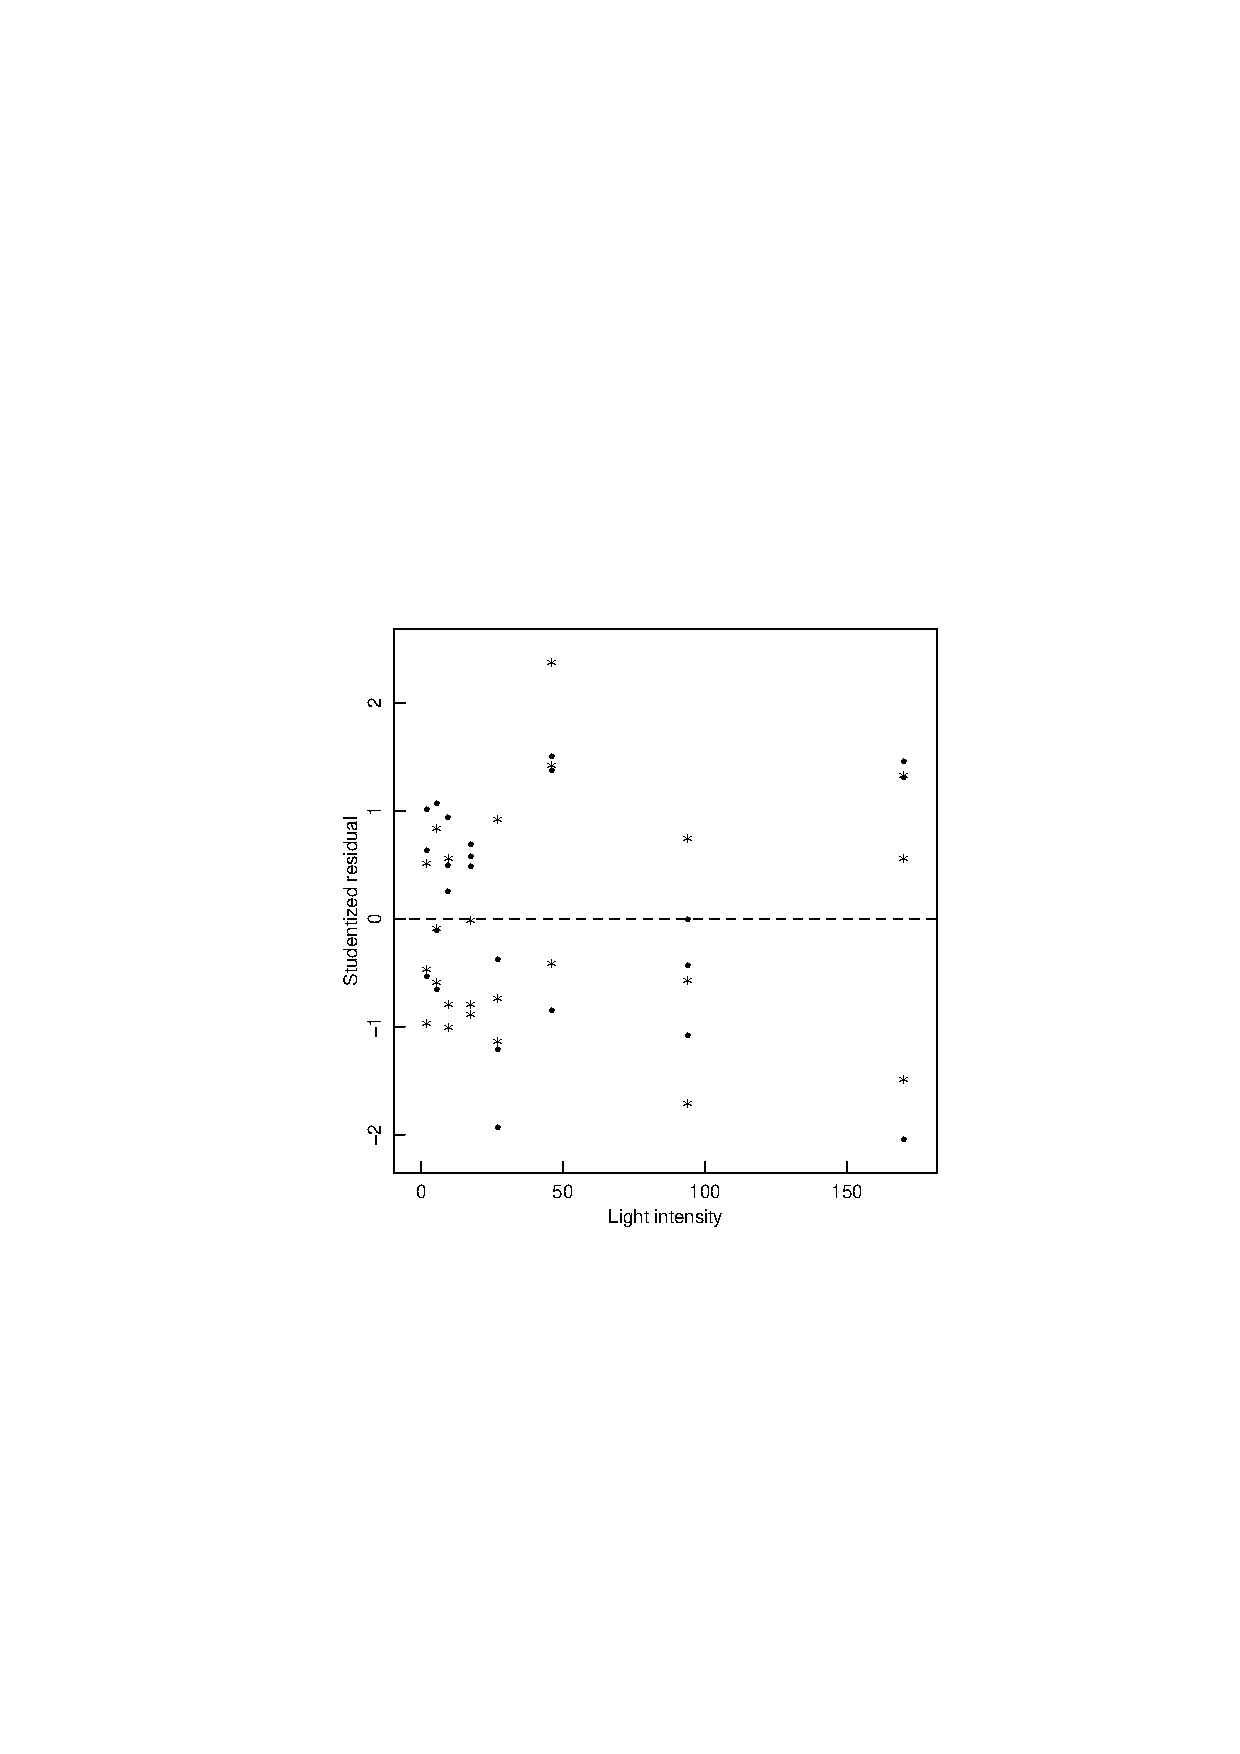
\includegraphics{3NITres3}}%,height=3in}}
  \caption{Studentized residuals from the 4-parameter quadratic
    Michaelis--Menten model plotted versus light intensity.  Day 1
    data are shown as * and day 2 data as $\cdot$.}
  \label{fig:NITres3}
\end{figure}
Figure~\ref{fig:NITres3}, attest to the adequacy of the model.
Furthermore, a lack of fit analysis, shown in
Table~\ref{tbl:qmic4lof}, suggests that the model is adequate.
\begin{table}
  \caption{Lack of fit analysis for the 4-parameter quadratic
    Michaelis--Menten model fitted to the nitrite utilization data.}
  \label{tbl:qmic4lof}
  \begin{center}
    \begin{tabular}{lccccc}\hline
      &\multicolumn{1}{c}{Sum of}&\multicolumn{1}{c}{Degrees}
      &\multicolumn{1}{c}{Mean}\\
      &\multicolumn{1}{c}{Squares} &\multicolumn{1}{c}{of} &
      \multicolumn{1}{c}{Square}\\
      \multicolumn{1}{c}{Source} & \multicolumn{1}{c}{$( 10^6 )$}
      &\multicolumn{1}{c}{Freedom} & \multicolumn{1}{c}{$( 10^6 )$} &
      \multicolumn{1}{c}{F Ratio} & \multicolumn{1}{c}{$p$ Value}\\ \hline
      Lack of fit&10.63&12&0.886&1.28&0.28\\
      Replications&22.21&32&0.694\\ \hline
      Residuals&32.84&44&0.746\\ \hline
    \end{tabular}
  \end{center}
\end{table}

Note that the parameter $\phi_{1}$ is now apparently
significantly different from 0, with an approximate
$t$ ratio of $-2.8$, confirming our earlier
suspicion that there was a difference between days.
This parameter was not significantly different from 0 in the
6-parameter model, which is further evidence for the 6-parameter
model being overparametrized and hence the parameter
approximate standard errors being artificially inflated, causing
nonsignificant $t$ ratios.

The parameter approximate correlation matrix for the quadratic
Michaelis--Menten 4-parameter model shown in
Table~\ref{tbl:3.6}
reveals that several of the correlations are very large.
This is not unusual in nonlinear regression, and is induced by a
combination of the form of the expectation function and the
design used.
For example, for a Michaelis--Menten model, no matter how good the
design is, it is impossible to obtain zero correlation between
the parameters because it is impossible to force the derivatives
to be orthogonal.
To see this, we note that the first column of
the derivative matrix, $\bv_{1}$, has elements
$x /( \theta_2 + x)$, and the second column,
$\bv_{2}$, has elements
${- \theta_1 x} / ( \theta_2 + x )^{2}$.
All the elements in $\bv_{1}$ are positive and all the
elements in $\bv_{2}$ are negative, and so the two vectors
$\bv_{1}$ and
$ - \bv_{2}$ will always tend to point in the same
direction in the response space.
Consequently, they will tend to be collinear.

As a final check on the model, the 3-parameter Michaelis--Menten
model
\begin{displaymath}
  f=\frac{(\theta_1+\phi_1x_2)x_1}{\theta_2+x_1}
\end{displaymath}
could be fitted and compared with the
4-parameter quadratic Michaelis--Menten model using an extra sum of
squares analysis to further substantiate the necessity for the parameter
$\theta_{3}$.
This was not done because the residuals for the original 3-parameter
Michaelis--Menten model were so badly behaved.

(Similar results and conclusions were reached for the exponential
difference model:  that is, a 4-parameter model with common
exponential parameters and scale factor, plus an incremental
parameter for day 2, was found to give an adequate fit.
Summary information on the fit is given in
Table~\ref{tbl:3.9},
\begin{table}
  \caption{Parameter summary for the 4-parameter exponential
    difference model fitted to the nitrite utilization data.}
  \label{tbl:3.9}
  \begin{center}
    \begin{tabular}{cccccccc} \hline
      &&\multicolumn{1}{c}{Standard} &&
      \multicolumn{4}{c}{Correlation}\\
      \multicolumn{1}{c}{Parameter} & \multicolumn{1}{c}{Estimate} &
      \multicolumn{1}{c}{Error} & \multicolumn{1}{c}{$t$ Ratio} &
      \multicolumn{4}{c}{Matrix}\\ \hline
      $\theta_{1}$&35115&8940&3.9&1.00\\
      $\theta_{2}$&0.01845&0.00317&5.8&--\/0.99&1.00\\
      $\theta_{3}$&0.00325&0.00120&2.7&0.99&--\/0.97&1.00\\
      $\phi_{1}$&$-2686$&1006&--2.7&--\/0.71&0.67&--\/0.68&1.00\\ \hline
    \end{tabular}
  \end{center}
\end{table}
and comparison with
the 6-parameter model in Table~\ref{tbl:3.10}.
\begin{table}
  \caption{
  Extra sum of squares analysis for the 6-parameter
  versus the 4-parameter exponential difference model
  fitted to the nitrite utilization data.
  }\label{tbl:3.10}
  \begin{center}
    \begin{tabular}{lccccc} \hline
      & \multicolumn{1}{c}{Sum of} & \multicolumn{1}{c}{Degrees} &
      \multicolumn{1}{c}{Mean}\\
      & \multicolumn{1}{c}{Squares} & \multicolumn{1}{c}{of} &
      \multicolumn{1}{c}{Square}\\
      \multicolumn{1}{c}{Source} & \multicolumn{1}{c}{$( 10^6 )$} &
      \multicolumn{1}{c}{Freedom} & \multicolumn{1}{c}{$( 10^6 )$} &
      \multicolumn{1}{c}{F Ratio} & \multicolumn{1}{c}{$p$ Value}\\ \hline
      Extra&0.37&2&0.19&0.23&0.80\\
      6-parameter&33.97&42&0.809\\ \hline
      4-parameter&34.34&44&0.780\\ \hline
    \end{tabular}
  \end{center}
\end{table}

The lack of fit analysis is given in Table~\ref{tbl:3.11}.
\begin{table}
  \caption{
  Lack of fit analysis for the 4-parameter exponential difference
  model fitted to the nitrite utilization data.}\label{tbl:3.11}
  \begin{center}
    \begin{tabular}{lccccc}\hline
      & \multicolumn{1}{c}{Sum of} & \multicolumn{1}{c}{Degrees} &
      \multicolumn{1}{c}{Mean}\\
      & \multicolumn{1}{c}{Squares} & \multicolumn{1}{c}{of} &
      \multicolumn{1}{c}{Square}\\
      \multicolumn{1}{c}{Source} & \multicolumn{1}{c}{$( 10^6 )$} &
      \multicolumn{1}{c}{Freedom} & \multicolumn{1}{c}{$( 10^6 )$} &
      \multicolumn{1}{c}{F Ratio} & \multicolumn{1}{c}{$p$ Value}\\ \hline
      Lack of fit&12.13&12&1.011&1.46&0.19\\
      Replications&22.21&32&0.694\\ \hline
      Residuals&34.34&44&0.780\\ \hline
    \end{tabular}
  \end{center}
\end{table}
In this case, the lack of fit ratio was 1.46, still not
significant, but slightly larger than for the quadratic
Michaelis--Menten model.)

\subsection{Comparing the Models}

To compare the nested models we have used incremental parameters
and the extra sum of squares principal, but they can not be used
to compare the quadratic Michaelis--Menten and the exponential
difference models.
Our first approach was to the researchers, asking them whether
one model was preferred on scientific grounds.
In this case, the researchers had no
preference, and so we simply presented them
with the results for both models.
Because the lack of fit ratio and the residual mean squares were
smaller, we had a slight preference for the Michaelis--Menten
model.
In Figure~\ref{fig:NITconfband}
\begin{figure}
  \centerline{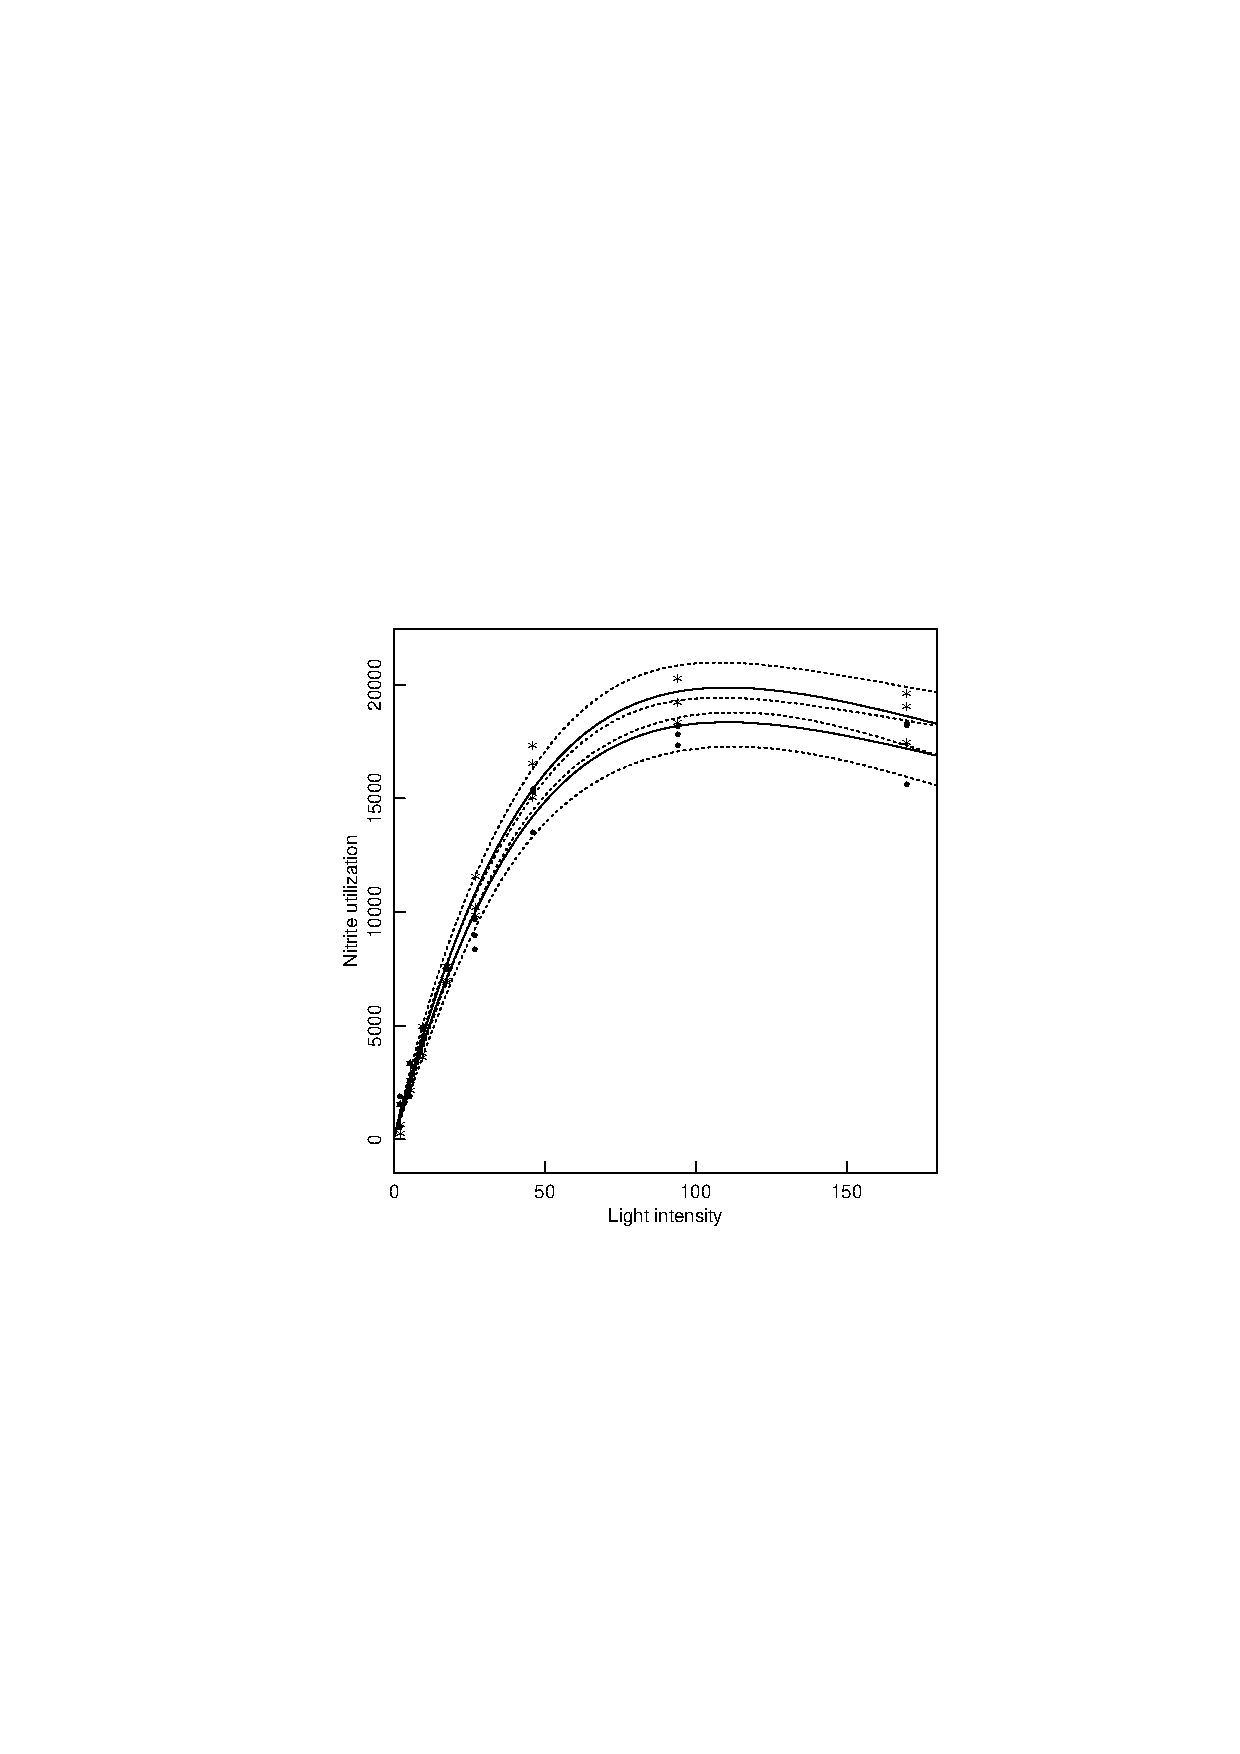
\includegraphics{3NITconfband}}%,height=3in}}
  \caption{Plot of nitrite utilization versus light intensity together
    with the fitted curves (solid lines) and the 95\% approximate
    inference bands (dotted).  Data for day 1 are shown as * and for
    day 2 as .}
  \label{fig:NITconfband}
\end{figure}
we show the nitrite utilization data together with
the fitted curve and the approximate 95\% confidence bands for the
4-parameter quadratic Michaelis--Menten model.

\subsection{Reporting the Results}

A brief report was prepared for Professors Elliott and
Peirson, along the lines of Section 3.12.
The major finding of interest was the need for a model which rose
to a peak rather than to an asymptote.
This was not expected, at least at such a low light level.
As part of our report, we recommended additional experiments be
run, especially at higher light intensities, in order to verify
the need for a model which rises to a peak rather than approaching an
asymptote, and to help discriminate between the two competing models.
It was further suggested that future experiments involve fewer
levels at low light intensity to reduce effort.

\section{Experimental Design}

So far we have concentrated more on the analysis of data
than on the design of experiments to produce good data, although
we believe that good experimental design is vital to
scientific progress.
The reason for the prime importance of experimental design is
that \emph{the information content of the data is established
when the experiment is performed}, and no amount of sensitive data
analysis can recover information which is not present in the
data.

One reason for our emphasizing analysis rather than design is
that we usually have to deal with data that have been
obtained without the benefit of good statistical design.
Another reason is that, while good experimental design is
extremely valuable, it is necessary to know how to analyze data
in order to appreciate what ``good experimental design'' is.

\subsection{General Considerations}
\index{experimental design!general considerations}

Experimentation is fundamental to scientific learning, which we
may characterize as \emph{reducing ignorance}.
At any stage of research, we are in a position of having data,
and of being able to explain part of that data, and
as the research proceeds, we are able to account for, or
explain, more of the data.
For example, a chemical engineer trying to learn about how a
particular product is produced would know very little initially
about the factors and the chemical reactions involved.
As she proceeds, planning and running experiments under various
conditions, she would endeavor to find out, at each stage, what
the important factors are, and how they affect the response.
Initially, she would be involved in empirical ``screening designs''
to try to isolate those factors which are most influential in
affecting the response, probably using \emph{factorial} or
\emph{fractional factorial} designs
\cite{box:hunt:hunt:1978}.
%\glossary{ Box, G.E.P.}
%\glossary{ Hunter, J.S.}
%\glossary{ Hunter, W.G.}
If she was interested in optimizing some characteristic, she
might then proceed to \emph{response surface} designs
\cite{box:drap:1987,box:hunt:hunt:1978}.
%\glossary{ Draper, N.R.}
%\glossary{ Box, G.E.P.}
%\glossary{ Hunter, J.S.}
%\glossary{ Hunter, W.G.}
Later on, perhaps to fine tune the product or to gain better
understanding of the mechanisms involved, she would move from
empirical models and their associated strategies to mechanistic
(usually nonlinear) models.
It is this aspect of experimental design which we consider in
this section.

We assume initially that the experimenter has a well-defined
\emph{form} for the expectation function relating the
factors to the response, and that the objectives
of the experiments are to provide the necessary and adequate
\index{experimental design!objectives}
information to:
estimate the parameters of interest in the model with
  \begin{enumerate}
    \item accuracy (i.e. small bias),\\
          precision (i.e. small variance), and
verify the assumptions about
    \item the expectation function,\\
          the disturbance model.
  \end{enumerate}

As was the case for estimation, it is helpful first to
discuss the linear situation.
Accordingly, in the following section we present a brief review
of experimental design for linear expectation functions.
For a more comprehensive presentation, see
\citeasnoun{box:hunt:hunt:1978},
%\glossary{ Box, G.E.P.}
%\glossary{ Hunter, J.S.}
%\glossary{ Hunter, W.G.}
\citeasnoun{davi:1956}, and \citeasnoun{coch:cox:1957}; and
%\glossary{ Davies, O.L.}
%\glossary{ Cochran, W.G.}
%\glossary{ Cox, G.M.}
for general considerations on the planning of experiments,
\citeasnoun{box:drap:1959} and
%\glossary{ Box, G.E.P.}
%\glossary{ Draper, N.R.}
\citeasnoun{drap:smit:1998}.
%\glossary{ Draper, N.R.}
%\glossary{ Smith, H.}
A thorough review of optimal designs is given in
\citeasnoun{stjo:drap:1975},
%\glossary{ St.John, R.C.}
%\glossary{ Draper, N.R.}
\citeasnoun{coch:1973}, and \citeasnoun{stei:hunt:1984}.
%\glossary{ Cochran, W.G.}
%\glossary{ Steinberg, D.M.}
%\glossary{ Hunter, W.G.}
\citeasnoun{hami:watt:1985} discussed designs using second order
%\glossary{ Hamilton, D.C.}
%\glossary{ Watts, D.G.}
derivatives, and
the geometry of experimental designs was discussed in
\citeasnoun{silv:titt:1973}.
%\glossary{ Silvey, S.D.}
%\glossary{ Titterington, D.M.}

Before considering the more technical details of experimental
design, we offer some comments which help ensure
attainment of the general objectives (1) and (2) above.

With regard to providing accurate and precise estimates of the
parameters, it is helpful to recognize that an experimental
design involves choosing the values of the factors for a selected
number of experimental cases (or runs).
It is therefore important that the number of cases be large
enough to ensure attainment of the specific objectives of the experiment.
For example, if an expectation function involves five
parameters, there will have to be at least five distinct
experimental conditions.
It is equally important to limit the number of experiments done
at any one time.
That is, one should not construct an extremely large design and
then proceed slavishly to follow that design to its completion.
Due account should be taken of what is learned at each stage of
the experiment, and this information should be exploited in the
design of the next stage.
The number of experiments which should be run in a \emph{block}
will depend on the number of factors and the type of experiment
being run, of course, but blocks of size 10 to 20 are usually
informative and manageable.

The choices of the factor settings should be such that they are in
useful and appropriate ranges of the factors.
That is, the factors should be located near sensible
values which will permit use of the parameter estimates in future
investigations, and the levels of each factor should be spread
out enough so that the effect of each factor will be revealed in
spite of the inherent variability of the response.

With regard to
verifying the assumptions about the expectation
function, it is important to provide \emph{replications}
\index{replication}
to enable testing for lack of fit or inadequacy of the
expectation function.
It is also important, when possible, to \emph{randomize}
the order of the
\index{randomization}
experiments, to ensure that the expectation function is appropriate.
(If there are unsuspected factors operating, randomizing will tend
to cause their effects to appear as increased variability rather
than as incorrect parameter estimates, as discussed in Section 1.3.)

With regard to
verifying the assumptions about the disturbance
model, replications are again important.
As discussed in Section 1.3, replications enable one to test for
constancy of variance and to determine a variance stabilizing
transformation if the variance is deemed not constant.
Randomizing will also tend to ensure that all of the
assumptions concerning the disturbances will be appropriate, as
discussed in Section 1.3.
Once again, we see the importance and power of randomizing.

In summary, \emph{statistical analysis} is concerned with the efficient
extraction and presentation of the information embodied in a data set,
while \emph{statistical experimental design}
is concerned first with
ensuring that the important necessary information is embodied in a data
set,
and second with making the extraction and presentation of that
information easy.

\subsection{The Determinant Criterion}
\index{experimental design!for linear expectation functions}

Consider the linear model (1.1)
\begin{displaymath}
\bY=\bX \bbeta+\bZ
\end{displaymath}
with the usual assumptions (1.2) and (1.3) about the disturbances
$\bZ$,
\begin{displaymath}
\mbox{\rm E} [ \bZ ] =  {\bf 0} 
\end{displaymath}
\begin{displaymath}
\mbox{\rm Var} [ \bZ ] = \sigma^2 \bI
\end{displaymath}
For a linear regression model, a row of the derivative matrix $\bX$
depends only on the choice of the $K$ design variables, where the
design variables determine such characteristics as when the run
is taken, at what pressure, at what temperature, etc.
An individual entry in the derivative matrix is calculated from the
values of the design variables.
For any choice of the design variables generating a derivative matrix
\index{derivative matrix}
$\bX$, the parameters
$\bbeta$ will have a joint inference region whose volume
is proportional to $| \bX \trans \bX |^{{-} 1/2}$.
Thus, a logical choice of design criterion is to choose the
design points so that the volume of the joint inference
region is minimized
\index{experimental design!determinant criterion}
\index{experimental design!D-optimal}
\index{D-optimal!design criterion}
\cite{wald:1943}.
%\glossary{ Wald, A.}
Since the power $-1/2$ is inconsequential,
Wald proposed
maximizing the determinant $D = | \bX \trans \bX |$, and
designs which satisfy this criterion are called \emph{D-optimal}
designs.
The criterion is referred to as the \emph{determinant criterion}.
\index{determinant!design criterion}

From a geometric point of view, the determinant criterion implies
\index{geometry!of experimental design determinant criterion}
that we should choose the columns of $\bX$ so that each
vector is as long as possible ($\norm \bx_p \norm^{2}$ is as
large as possible, $p=1 ,2 ,\ldots, P$), and try to make the
vectors orthogonal ($\bx_p \trans \bx_{q=0} ,p!=q$).
The former ensures that the expectation plane will be well supported
in the response space, and that the parameter lines will be widely
spaced on the expectation plane.
Consequently the disturbances, whose variance is beyond our
control, will have small effect, thereby producing a joint region
in the parameter space with small volume.
The latter ensures that the parameter estimates associated with
the factors will not be correlated.
That is, changes in the response will be correctly associated
with changes in the appropriate causative factor, and not
attributed to other factors.

The two requirements of long length and orthogonality
of the derivative vectors
ensure that a disk on the expectation plane will map to a small
ellipse in standard position on the parameter plane.

\index{experimental design!for nonlinear expectation functions}
The determinant criterion was applied to nonlinear expectation
functions by
\citeasnoun{box:luca:1959} who used, in place of the $\bX$
%\glossary{ Box, G.E.P.}
%\glossary{ Lucas, H.L.}
matrix, the derivative matrix $\bV^{0}$ evaluated at
some initial parameter estimates $\btheta^0 $.
That is, in nonlinear design, the $D$-optimal criterion is modified to
maximize
\index{D-optimal!design criterion}
\begin{displaymath}
D = | {\bV^0}\trans\bV^0 |
\end{displaymath}

The design of an experiment depends on the stage at which the
researcher is in an investigation.
When only the form of the model is known, but not the parameter values,
as could be the case in enzyme kinetics or in biochemical oxygen demand
studies, the researcher would be concerned with choosing the values of
the factors to produce good parameter estimates.
These are called ``starting designs.''
Later on in an investigation, the researcher might wish to design an
experiment to improve the precision of estimates of some or all of the
parameters, exploiting data already obtained.
Such designs are called ``sequential designs,''
and, when special interest is attached to a subset of the parameters,
``subset designs.''

\subsection{Starting Designs}
\index{experimental design!starting}

\citeasnoun{box:luca:1959}
%\glossary{ Box, G.E.P.}
%\glossary{ Lucas, H.L.}
proposed starting designs consisting of $P$ points for a
$P$-parameter model, and therefore simplified the criterion
(\ref{eqn:6.1}) to that of maximizing $| \bV^0 |$.
Geometrically, the determinant criterion ensures that the
\index{determinant!design criterion}
expectation surface is such that large regions on the tangent
plane at $\boeta ( \btheta^0 )$ map to small regions
in the parameter space.
When more than $P$ points are to be chosen, the
$D$-optimal design usually results in replications of
$P$ distinct design points \cite{box:1968}, and these design points
%\glossary{ Box, M.J.}
are those that would be chosen as $D$-optimal with $N = P$.
We therefore consider starting designs as having only $P$ runs.

\begin{example}\label{mic:dopt}
To illustrate the choice of a starting design, we consider the case of
enzyme kinetics, which are assumed to follow a Michaelis--Menten model.
We assume that the maximum allowable substrate
concentration is specified as
$x_{max}$, and that initial estimates of the parameters
$\btheta^{0}$ are given.

The derivatives of the expectation function, evaluated at the
initial parameter estimates $\btheta^{0}$, are
\begin{displaymath}
  \frac{x}{\theta_2^0+x}\frac{-\theta_1^0x}{(\theta_2^0+x)^2}
\end{displaymath}
and so the determinant to be maximized is
\begin{eqnarray*}
  | \bV^0 |&=&\left|
  \begin{bmatrix}
    \frac{x_1}{\theta_2^0+x_1}&\frac{-\theta_1^0 x_1}{( \theta_2^0+x_1 )^2}\\
    \frac{x_2}{\theta_2^0+x_2}&\frac{-\theta_1^0 x_2}{( \theta_2^0+x_2)^2}
  \end{bmatrix}\right|\\
  &=&\frac{\theta_1^0 x_1 x_2| x_1-x_2 | }{ ( \theta_2^0+x_1 )^2 (
    \theta_2^0+x_2 )^2}
\end{eqnarray*}
The modulus of this determinant is maximized when
\begin{displaymath}
  x_1=x_{\mbox{\rm max}}\quad\text{and}\quad
  x_2=\frac{\theta_2^0}{1+2(\theta_2^0/x_{\text{max}})}\approx\theta_2^0
\end{displaymath}
The determinant criterion therefore places the design points so
as to tie down the asymptote ($\theta_{1}$) by performing one
experiment at the maximum concentration, and to tie down the
half-concentration by performing the other experiment near the assumed
half-concentration.

It is instructive to compare the $D$-optimal design with the
dilution design used by \citeasnoun{trel:1974}.
%\glossary{ Treloar, M.A.}
The dilution design used $x_{\text{max}}=1.1$ and five dilutions by
approximately one-half, with duplications, giving a total of 12 runs.
With the same number of runs, the $D$-optimal design would consist of 6
replications at $x_{max}$ and 6 replications at
$x_2=\theta_2^0 /[1+2 ( \theta_2^0 / x_{\text{max}})]$.
We take $\theta_2^0  =  0.1$ as a reasonable starting estimate,
and so the design is $x_1  =  1.1$, $x_2  =  0.085$.
In Figure \ref{fig:MICdesign}
\begin{figure}
  \centerline{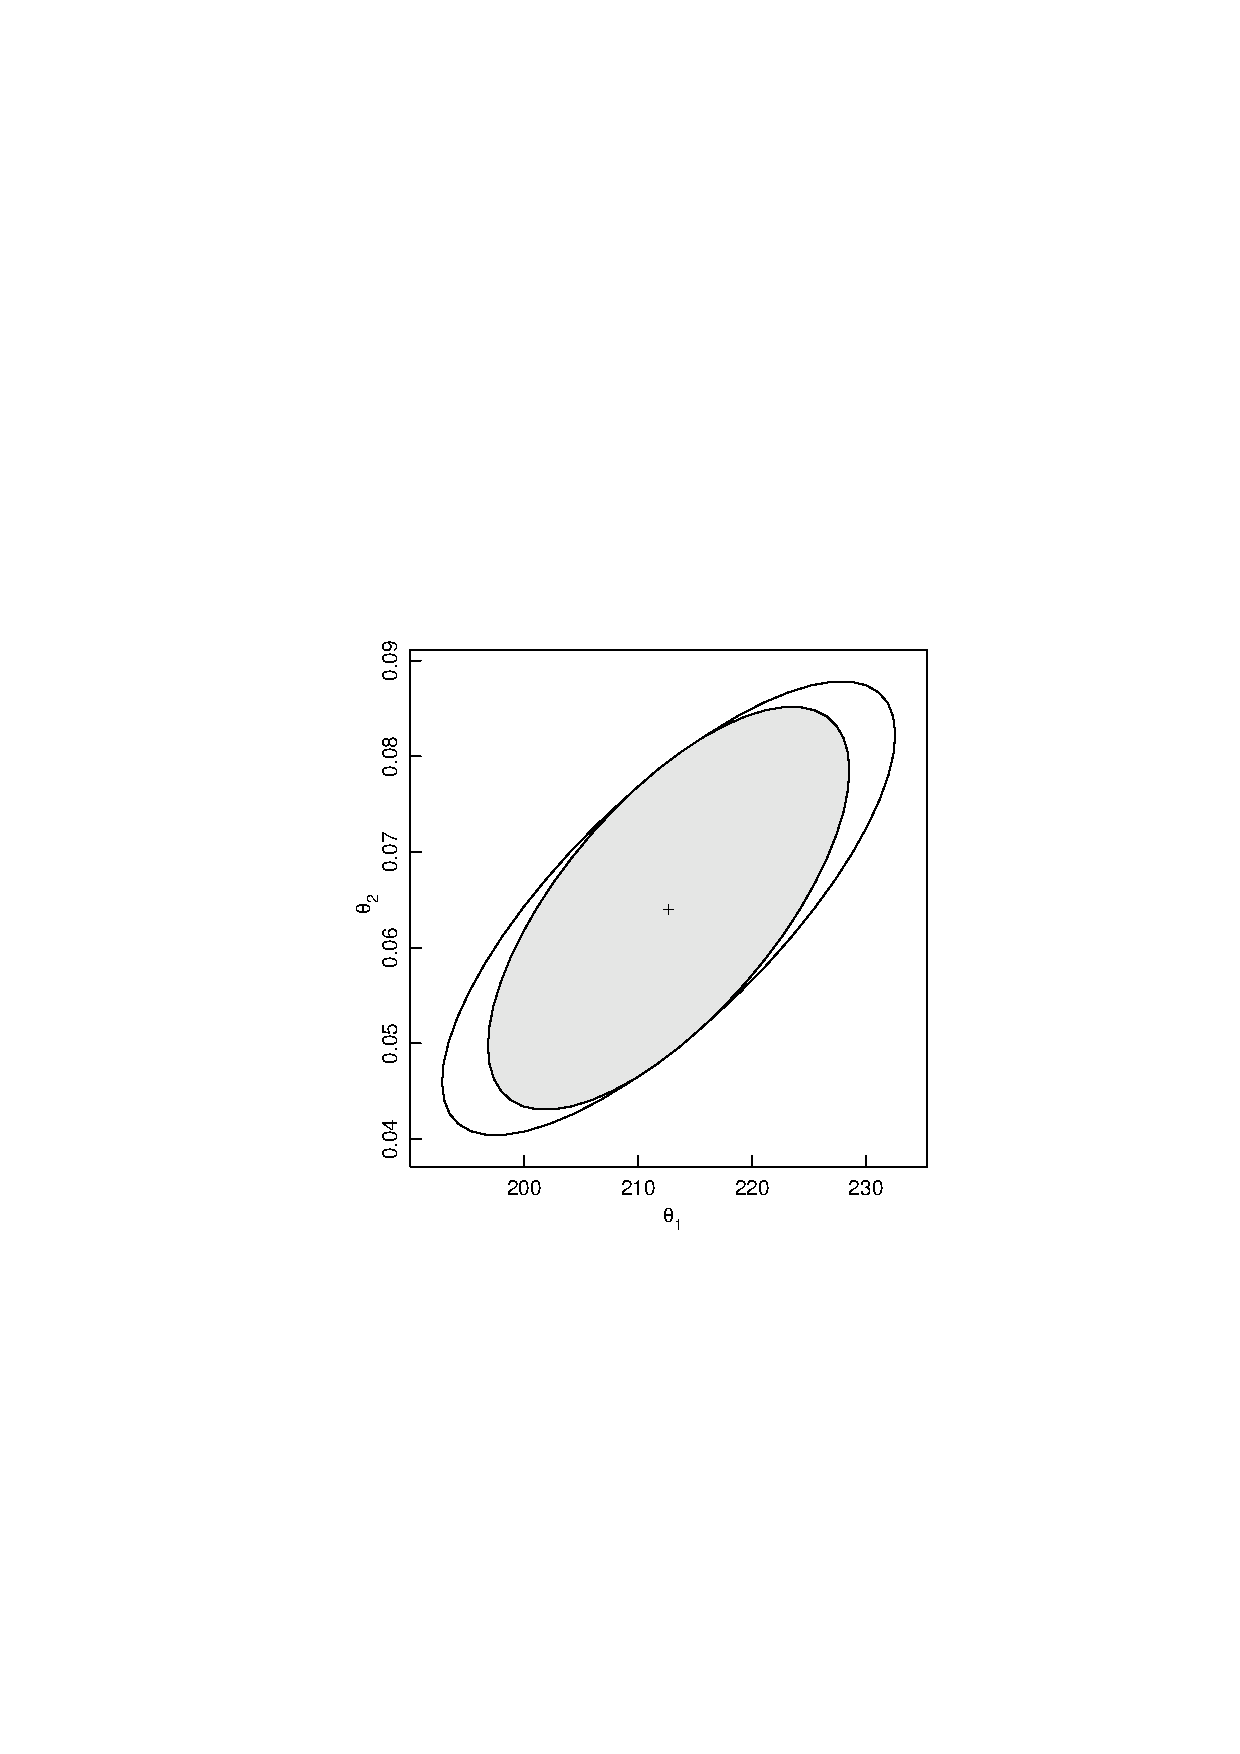
\includegraphics{3MICdesign}}%,height=3in}}
  \caption{Comparison of 95\% approximate inference regions for two
    designs for the Puromycin data.  The larger region results from
    the dilution design used, and the shaded region results from a
    $D$-optimal design.}
  \label{fig:MICdesign}
\end{figure}
we plot the linear approximation 95\% confidence
region for the dilution design and data together with the linear
approximation confidence region for the $D$-optimal design assuming that
both designs gave the same parameter estimates and residual variance.
We see that the $D$-optimal design does indeed give a smaller joint
confidence region and smaller confidence intervals.
In addition, the correlation between the parameters is lower.
However, the gain in precision from using the $D$-optimal design would
have to be balanced against any loss of information about lack of fit.

Note that the design does not depend on the conditionally linear
parameter $\theta_{1}$, which is true in general for conditionally
linear parameters, as shown in Section 3.14.6.
\end{example}

The determinant criterion provides an objective basis for
determining $P$-point designs for $P$-parameter models, but the
design strategy should not be applied blindly.
The criterion was derived on the basis that the expectation
function is \emph{known}, and provides only $P$ design points to
estimate the $P$ parameters.
Replications at these $P$ design points are useful because
\index{replication}
they provide information concerning constancy of
variance, but they cannot provide information about lack of fit.
It might be useful, therefore, to perform additional experiments
at other design points in order to detect lack of fit.
In light of these considerations, the dilution design strategy is
eminently sensible, especially given its high level of performance
as demonstrated in the above example.
\subsection{Sequential Designs}
\index{experimental design!sequential}

In many situations, some experiments will already have been
done to check if the equipment is functioning properly, or to screen
possible models, as described in \citeasnoun{box:hunt:1965}.
%\glossary{ Box, G.E.P.}
%\glossary{ Hunter, W.G.}
In other situations, it may be possible to perform and analyze the
result from a single experiment quite rapidly.
In these situations, it is possible to obtain even better parameter
estimates by designing the experiments sequentially;
that is, an experimental run is designed, the data are collected and
analyzed, and the
design for the next run is obtained by maximizing
$| \bV_1 \trans \bV_1 |$ with respect to the design variables,
$\bx_{N+1}$, where
\begin{displaymath}
\bV_1= \begin{pmatrix}\bV_0\\\bv_{N+1}\end{pmatrix}
\end{displaymath}
and $\bv_{N+1}$ is the gradient vector
$\partial f / \partial \btheta \trans$
evaluated at the least squares estimates from the $N$ runs already made.

\begin{example}\label{iso:dopt}
To illustrate sequential design, we consider the model and data set
from Example Isomerization 1.
The correlations between the parameters are very high, and the linear
approximation confidence regions include negative values for the
equilibrium constants.
We would therefore like to design experiments to provide better
precision in the parameter estimates.

The design points are determined by the values of the partial pressure
of hydrogen, $x_{1}$, the partial pressure of $n$-pentane, $x_{2}$,
and the partial pressure of isopentane, $x_{3}$.
In the previous runs these variables have ranged from about
100 to 400 for $x_{1}$, 75 to 350 for $x_{2}$, and 30 to
150 for $x_{3}$, so we use these limits to define a reasonable
region within which to design further runs.
We begin by evaluating the sequential
$D$-optimal design criterion at the original design points and at
sequential design points at the corners of the region.
This gives the values in Table \ref{tbl:ISOdopt}.
  \begin{table}
\begin{center}
\begin{tabular}{llrc}\hline
 \multicolumn{3}{c}{Factor}  & \multicolumn{1}{c}{Criterion}\\
& & & \multicolumn{1}{c}{$D$}\\
\multicolumn{1}{c}{$x_{1}$} & \multicolumn{1}{c}{$x_{2}$} & \multicolumn{1}{c}{$x_{3}$} & \multicolumn{1}{c}{$10^{6}$} \\ \hline
100&100&30&4.63\\
400&100&30&1.95\\
100&350&30&9.44\\
400&350&30&3.99\\
100&100&150&1.82\\
400&100&150&1.82\\
100&350&150&3.98\\
400&350&150&2.42\\ \hline
\end{tabular}
\end{center}
  \end{table}
The combination which optimizes the $D$-optimal criterion is low
$x_{1}$ (100), high $x_{2}$ (350), and low $x_{3}$ (30).
Examination of nearby values confirms that the
corner is a local optimum, and since a coarse grid search of the
design region did not reveal any optima in the interior,
we choose this corner as the design point for the next run.
\end{example}

\subsection{Subset Designs}
\index{experimental design!subset}

When only a subset of the parameters
$\btheta$ is of interest, the design criterion is modified as suggested
in \citeasnoun{box:1971:biok} and \citeasnoun{hill:hunt:1974}.
%\glossary{ Box, M.J.}
%\glossary{ Hill, W.J.}
%\glossary{ Hunter, W.G.}
We assume that the parameters have been ordered so the first $P_{1}$ 
parameters are the nuisance parameters and the trailing $P_{2}$
parameters are the parameters of interest, and we
partition the vector $\btheta \trans$ as
$( \btheta_1 \trans | \btheta_2 \trans )$
and the matrix $\bV^{0}$ as $[ \bV_1^0| \bV_2^0 ]$.
Then the variance--covariance matrix of the $P_{2}$
parameters is proportional to $\bD_{2,2}$, where
\begin{eqnarray*}
  \bD&=&({\bV^0}\trans \bV^0 )^{-1}\\
  % && = \left[  \matrix {
  % \matrix{{{\bV_1^{0}}\trans \bV_1^0}
  % \cr{{\bV_2^{0}}\trans \bV_1^0}}
  % \matrix{{{\bV_1^{0}}\trans \bV_2^0}
  % \cr{{\bV_2^{0}}\trans \bV_2^0}}
  % }\right]^{-1}\\
  % && = \left[ \matrix {
  % \matrix { \bD_{1,1} \cr \bD_{1,2} \trans }
  % \matrix { \bD_{1,2} \cr \bD_{2,2} }
  % }\right]
\end{eqnarray*}
and so the $D$-optimal criterion is changed to minimization of
\begin{displaymath}
D_S = | \bD_{2,2} |
\end{displaymath}
which is equivalent to maximizing
\begin{displaymath}
\frac{ | { \bV^0 } \trans \bV^0 |}{ | { \bV_1^0 } \trans \bV_1^0 | }
\end{displaymath}

\begin{example}\label{iso:subset}

To illustrate subset design, we consider the model, data set, and
design region from Example Isomerization \ref{iso:dopt}, and treat the
situation in which we wish to improve the estimates of $\theta_{2}$,
$\theta_{3}$, and $\theta_{4}$.
Evaluation of $D_{S}$ at the corners of the same region gives the results
in Table \ref{tbl:ISOsubset},
\begin{table}
  \caption{
  Sequential $D$-optimal subset design criteria for the isomerization model,
  evaluated at the corners of the design region.
  }\label{tbl:ISOsubset}
  \begin{center}
    \begin{tabular}{llrc}\hline
      \multicolumn{3}{c}{Factor}  & \multicolumn{1}{c}{Criterion}\\
      & & & \multicolumn{1}{c}{$D$}\\
      \multicolumn{1}{c}{$x_{1}$} & \multicolumn{1}{c}{$x_{2}$} &
      \multicolumn{1}{c}{$x_{3}$} & \multicolumn{1}{c}{$10^{6}$} \\ \hline
      100&100&30&8.77\\
      400&100&30&3.90\\
      100&350&30&13.11\\
      400&350&30&7.08\\
      100&100&150&3.69\\
      400&100&150&3.68\\
      100&350&150&7.39\\
      400&350&150&4.70\\ \hline
    \end{tabular}
  \end{center}
\end{table}
which produce similar conclusions and the
same design point as in Example Isomerization \ref{iso:dopt}.

\end{example}

\subsection{Conditionally Linear Models}
\index{conditionally linear!model}
\index{experimental design!for conditionally linear model}

It is awkward to have to specify initial estimates of the parameters
$\btheta$ before an experimental design can be obtained, since, after
all, the purpose of the experiment is to determine parameter estimates.
In Examples Puromycin \ref{mic:dopt} and Isomerization \ref{iso:dopt},
we saw that the $D$-optimal design was not affected by the value of a
conditionally linear parameter.
For most models with conditionally linear parameters, the
locations of the $D$-optimal design points do not depend
on the conditionally linear parameters
\cite{hill:1980,khur:1984},
%\glossary{ Hill, P.D.H.}
%\glossary{ Khuri, A.I .}
so the design problem is simpler.

The easiest type of conditionally linear model to demonstrate this for
is that with only one conditionally linear parameter,
so the function can be written
\begin{displaymath}
f ( \bx , \btheta ) = \theta_1  g ( \bx , \btheta_{-1} )
\end{displaymath}
for some function $g$ where
$\btheta_{-1} = ( \theta_2 ,\ldots, \theta_P ) \trans$.
This includes the Michaelis--Menten, BOD, and isomerization models.
The gradient of the model function can then be written
\begin{displaymath}
  \frac{\partial f}{\partial\btheta\trans}=\left(g(\bx,\btheta_{-1}),
    \frac{\partial g}{\partial\btheta_{-1}\trans}\right)
  \begin{bmatrix}
    1 & 0\\
    \bm0 &\theta_1 \bI
  \end{bmatrix}
\end{displaymath}
which isolates the dependence of $\theta_{1}$ from any dependence
upon $\bx$.
Using (\ref{eqn:clfact}), the derivative matrix $\bV$ can be written
\begin{displaymath}
  \bV = \bH ( \bx , \btheta_{-1} )  \bB ( \theta_1 )
\end{displaymath}
where
\begin{displaymath}
\bB ( \theta_1 ) =
\begin{bmatrix}
  1 & 0\\
  \bm0 &\theta_1 \bI
\end{bmatrix}
\end{displaymath}
is $P \times P$, so the $D$-optimal criterion is
\begin{eqnarray*}
  | \bV \trans \bV |&=&| \bB \trans \bH \trans \bH  \bB |\\
  && =  | \bB |^2  | \bH \trans \bH |
\end{eqnarray*}
and, again, the dependence of $\theta_{1}$ is isolated from $\bx$.
Therefore, the design does not depend upon $\theta_{1}$.

In general, for conditionally linear models of the form
\begin{displaymath}
f ( \bx , \btheta ) = \theta_1 g_1 ( \bx , \btheta_{{-} \bL } )
+ \cdots + \theta_L g_L ( \bx , \btheta_{ - \bL } )
\end{displaymath}
where
$\btheta_{ - \bL } = ( \theta_{L+1} ,\ldots, \theta_P ) \trans$,
the
$D$-optimal design will not depend on the conditionally linear parameters
$( \theta_1 ,\ldots, \theta_L ) \trans$ if $\bV$ can be factored as in
(\ref{eqn:dfact}), provided $\bB$ is square.
The condition that the matrix $\bB$ is square was not explicitly stated
in \citeasnoun{hill:1980}, nor was it emphasized in
%\glossary{ Hill, P.D.H.}
\citeasnoun{khur:1984}, where it was shown that
%\glossary{ Khuri, A.I .}
conditionally linear parameters will usually affect subset designs.
This occurs because, for subset designs,
the design criterion involves the \emph{ratio}
of determinants of components of $\bV$, and
so the simple factorization above usually does not occur even if $\bB$ is
square.
\citeasnoun{khur:1984} gives conditions under which
%\glossary{ Khuri, A.I .}
the conditionally linear parameters do not affect designs for
subsets of parameters.

In the common situation where
each component of $\btheta_{-\bL} $ enters into only one of the
functions $g_i ,  i = 1 ,\ldots, L$, the derivatives can be factored
as in (\ref{eqn:dfact}).
For example, $D$-optimal designs for the sum of exponentials model
\begin{displaymath}
f ( x, \btheta ) = \theta_1 e^{ - \theta_2 x } +
\theta_3 e^{ - \theta_4 x } + \cdots +
\theta_{P-1} e^{ - \theta_P x }
\end{displaymath}
do not depend on the conditionally linear parameters.

\subsection{Other Design Criteria}

Precise parameter estimation is not the only objective used for
experimental design.
Methods have been proposed for constructing designs for discriminating
between possible model functions \cite{box:hill:1974} and for balancing
% \glossary{ Box, G.E.P.}
% \glossary{ Hill, W.J.}
the objectives of model discrimination and precise parameter estimation
\cite{hill:hunt:wich:1968}.
% \glossary{ Hill, W.J.}
% \glossary{ Hunter, W.G.}
% \glossary{ Wichern, D.}
The review article \cite{stei:hunt:1984} describes many of these
% \glossary{ Steinberg, D.M.}
% \glossary{ Hunter, W.G.}
criteria.
We also list several of the references for different experimental design
criteria for single response and multiresponse nonlinear models in the
bibliography.

\begin{problems}
  
  \prob Use the data from Appendix 4, Section A4.2 to fit the
  logistic model
  \begin{displaymath}
    f(x,\btheta)=\theta_1+\frac{\theta_2}{1+e^{-\theta_4(x-\theta_3)}}
  \end{displaymath}
  
  \subprob Plot the data versus $x=\log_{10}$ (NIF concentration).
  Note that you will have to make a decision about how to incorporate
  the zero concentration data. You may want to incorporate the actual
  NTD concentrations also.

  
  \subprob Give graphical interpretations of the parameters in the
  model, and use the plot to obtain starting values for each data set.
  
  \subprob Use the starting values in a nonlinear least squares
  routine to find the least squares estimates for the parameters for
  each data set.
  
  \subprob Use incremental parameters and indicator variables to fit
  all of the data sets together.
  
  \subprob Simplify the model by letting some of the parameters be
  common to all of the data sets.  Use extra sum of squares analyses
  to determine a simple adequate model.
  
  \subprob Write a short report about this analysis and your findings.
  
  \prob Use the data from Appendix 1, Section A1.14 to determine an
  appropriate sum of exponentials model.
  
  \subprob Plot the data on semilog paper and use the plot to
  determine the number of exponential terms to fit to the data.
  
  \subprob Use curve peeling to determine starting estimates for the
  parameters.
  
  \subprob Use the starting estimates from part (b) to fit the
  postulated model from part (a).
  
  \prob

  \subprob Use the plot from Problem 2.6 and sketch in the
  curve of steepest descent from the point
  $\btheta^{0}$.
  Hint: The direction of steepest descent is
  perpendicular to the contours.
  \subprob Is the direction of the Gauss--Newton increment
  close to the initial direction of steepest descent?
  \subprob Calculate and plot the Levenberg increment using a
  conditioning factor of $k=4$.
  \subprob Calculate and plot the Marquardt increment using a
  conditioning factor of $k=4$.
  \subprob Comment on the relative directions of the
  Gauss--Newton, Levenberg and Marquardt increment
  vectors.
  
  \prob Use the data from Appendix 4, Section A4.3 to determine an
  appropriate model and to estimate the parameters.
  
  \subprob Plot the concentration versus time on semilog paper,
  and use the plot to determine the number of
  exponential terms necessary to fit the data.
  \subprob Use the plot and the method of curve peeling to
  determine starting values for the parameters.
  \subprob Use a nonlinear estimation routine to estimate the
  parameters.
  
  \prob Use a nonlinear estimation routine and the data and model
  from Appendix 4, Section A4.4 to estimate the parameters.
  Take note of the number of iterations required and any
  difficulties you encounter in each attempt.
  
  \subprob Use any approach you think is appropriate to obtain
  starting values for the parameters in the model.
  \subprob Use your starting values in a nonlinear estimation
  routine to estimate the parameters.
  If you achieve convergence, examine the parameter
  approximate correlation matrix, and comment on the
  conditioning of the model.
  \subprob Reparametrize the model by centering the factor $1/x_3$,
  and use the equivalent starting values from
  part (a) to estimate the parameters.
  If you achieve convergence, examine the parameter
  approximate correlation matrix, and comment on the
  conditioning of the model.
  What effect does this reparametrization have on the
  number of iterations to convergence?
  \subprob Reparametrize the model in part (a) using
  $\theta_{1=e}^{ \phi_1 }$ and $\theta_2=e^{\phi_2}$
  and the equivalent starting values from part (a)
  to estimate the parameters.
  If you achieve convergence, examine the parameter
  approximate correlation matrix, and comment on the
  conditioning of the model.
  What effect does this reparametrization have on the
  number of iterations to convergence?
  \subprob Reparametrize the model in part (b) using the same
  parametrization as in part (c) and the equivalent
  starting values from part (a) to estimate the
  parameters.
  If you achieve convergence, examine the parameter
  approximate correlation matrix, and comment on the
  conditioning of the model.
  What effect does this reparametrization have on the
  number of iterations to convergence?
  
  \prob Use a nonlinear estimation routine and the data and
  model from Appendix 4, Section A4.5 to estimate the
  parameters.
  Take note of the number of iterations required and
  any difficulties you encounter in each attempt.
  
  \subprob Use any approach you think is appropriate to obtain
  starting values for the parameters in the model.
  \subprob Use your starting values in a nonlinear estimation
  routine to estimate the parameters.
  If you achieve convergence, examine the parameter
  approximate correlation matrix, and comment on the
  conditioning of the model.
  \subprob Reparametrize the model in part (a) using $\theta_2
  e^{ - \theta_3 x }= e^{ - \phi_3 ( x - \phi_2 ) }$.
  If you achieve convergence, examine the parameter
  approximate correlation matrix, and comment on the
  conditioning of the model.
  What effect does this reparametrization have on the
  number of iterations to convergence?
  
  \prob 
  
  \subprob Show that the theoretical $D$-optimal starting
  design for the logistic model of Problem 3.1
  consists of $\bx=(-\infty,\theta_3-1.044/
  \theta_4,\theta_3+1.044/ \theta_4,+\infty)\trans$. 
  \subprob Interpret the choice of the design points
  graphically by plotting the logistic function versus
  $x$ and plotting the location of the design points
  on the $x$-axis.
  \subprob Plot the derivatives with respect to the parameters
  versus $x$ and use these plots to help interpret the
  choice of the design points.
  
\end{problems}

% Local Variables: 
% mode: latex
% TeX-master: "nraia2"
% End: 

\chapter{Multiresponse Parameter Estimation}
\prologue{Better is the enemy of the good.}{Voltaire}

In some experimental situations it is possible to measure more than
one response for each case.
In the analysis of such experiments, information from all the
measured responses can be combined to provide more precise
parameter estimation and to determine more
realistic models.
The information must be combined so as to reflect reasonable
assumptions on the behavior of the disturbance terms in the
measurements.

A determinant parameter estimation criterion for multiresponse
\index{multiresponse estimation}
data was derived by \citeasnoun{box:drap:1965} under the assumptions
%\glossary{ Box, G.E.P.}
%\glossary{ Draper, N.R.}
that the disturbance terms in different cases are uncorrelated but
the disturbance terms for different responses in the same case
have a fixed, unknown variance--covariance matrix.
In this chapter, we discuss this criterion and present a
generalization of the Gauss--Newton method to optimize it.
We also describe a convergence criterion for this optimization
method, and discuss modifications which should be made to the
method when there are singularities in the data or residual matrix.

\section{The Multiresponse Model}

We assume there are $M$ responses measured on each of $N$
experimental runs and that the models for the $M$ responses
depend on a total of $P$ parameters, $\btheta$, and write
\index{multiresponse estimation!model}
\begin{equation}\label{eqn:mrmodel}
  {\rm Y}_{nm} = f_m ( \bx_n , \btheta ) + {\rm Z}_{nm}
  \quad n = 1 ,\ldots, N\quad m = 1 ,\ldots, M
\end{equation}
where ${\rm Y}_{nm}$ is the random variable associated with the
measured value of the $m$th response for the $n$th
case, $f_{m}$ is the model function for the $m$th
response depending on some or all of the experimental settings
$\bx_{n}$ and on some or all of the parameters $\btheta$, and
${\rm Z}_{nm}$ is the disturbance term.

\begin{example}\label{pin:model}
\citeasnoun{box:hunt:macg:erja:1973} reported a multiresponse analysis of some
%\glossary{ Box, G.E.P.}
%\glossary{ Hunter, W.G.}
%\glossary{ MacGregor, J.F.}
%\glossary{ Erjavec, J.}
$\alpha$-pinene data originally analyzed by
\citeasnoun{fugu:hawk:1947}.
%\glossary{ Fuguitt, R.E.}
%\glossary{ Hawkins, J.E.}
In the experiment, $\alpha$-pinene, a component of turpentine, was
purified and heated to produce by-products.
Two sets of measurements were made, at temperatures of 189.5
and 204.5$^\circ$C.
In each experiment, the relative concentrations of $\alpha$-pinene
and three by-products were measured at each of eight times.
The relative concentration of a fourth by-product was imputed
from the other concentrations.
In this example, there are $M = 5$ responses and $N = 8$ cases.
The data for 189.5$^\circ$C are listed
in Appendix 1, Section A1.6, and plotted in Figure~\ref{fig:BHMEdata}.
  \begin{figure}
    \centerline{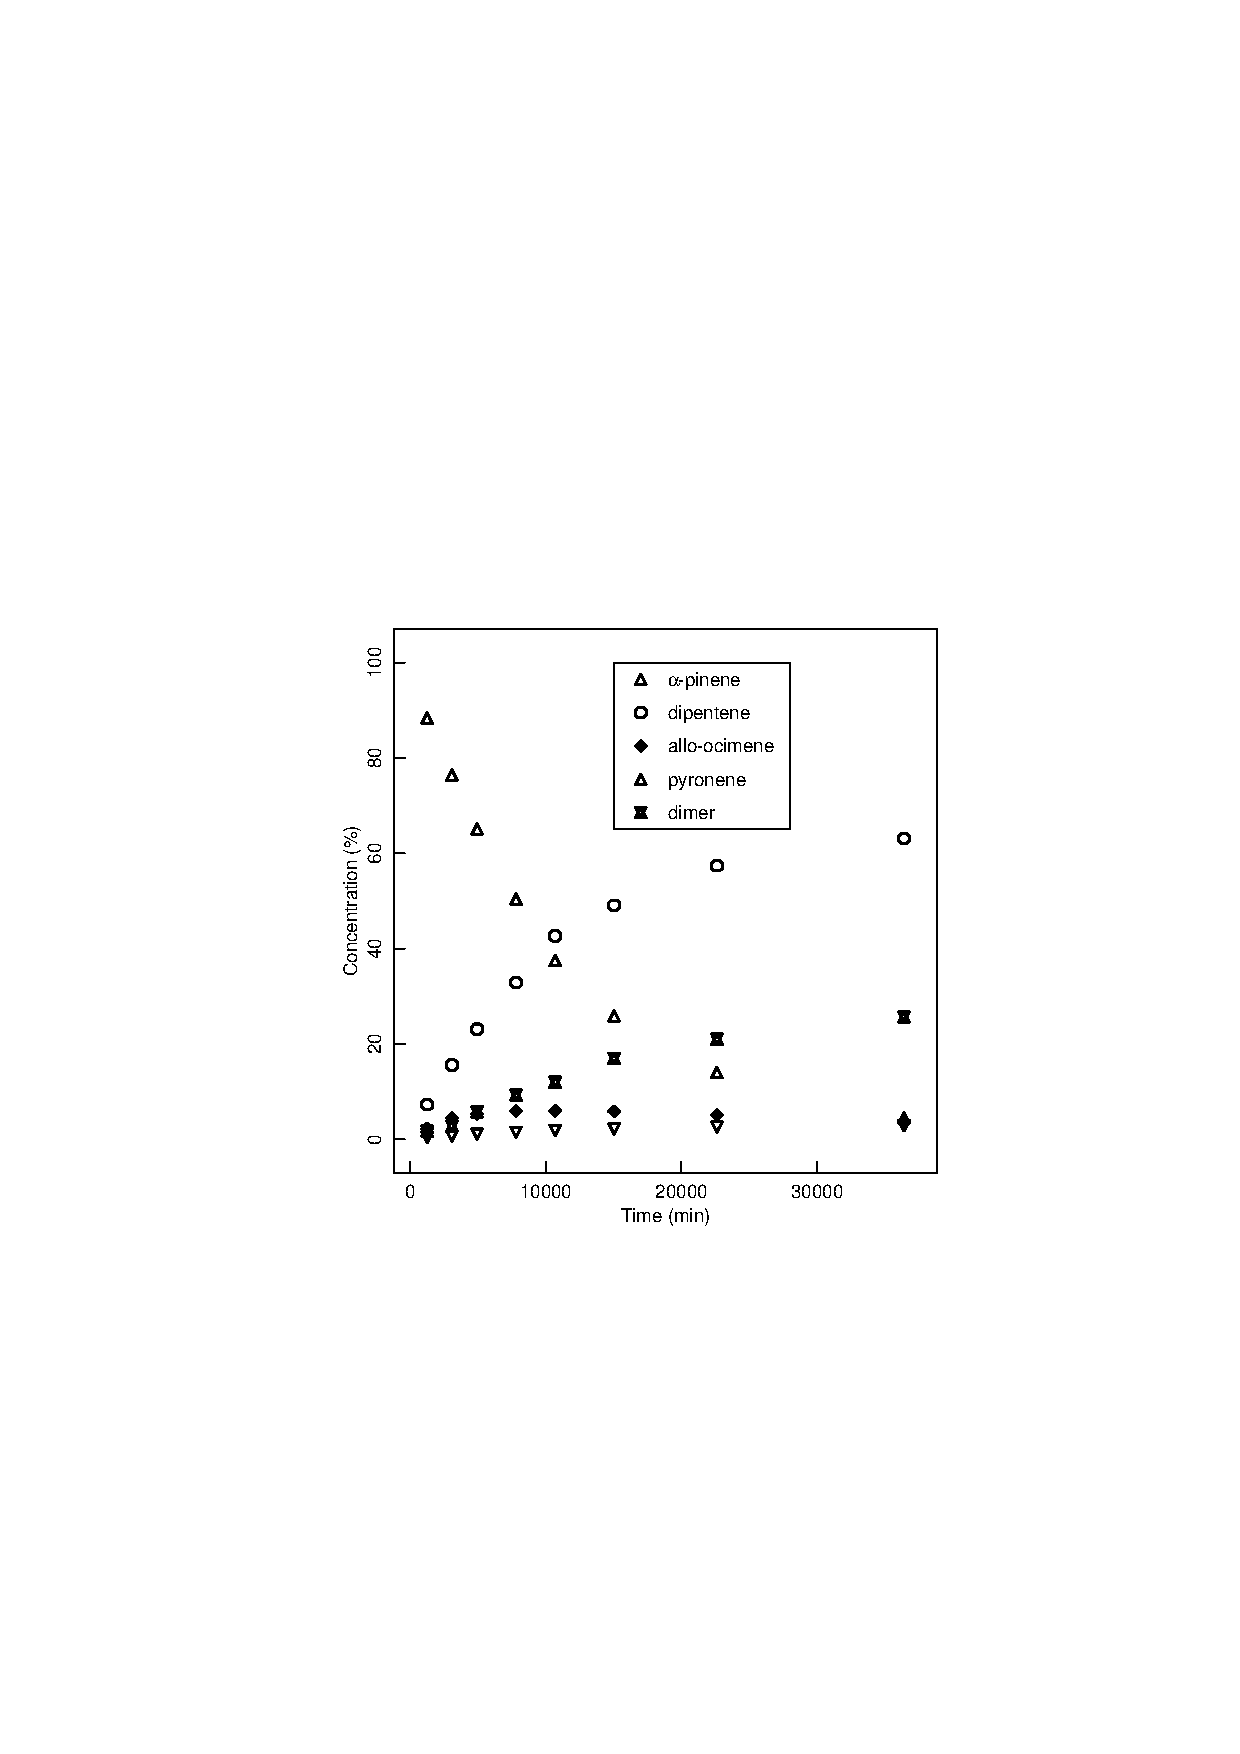
\includegraphics{4BHMEdata}}%,height=3in}}
    \caption{\label{fig:BHMEdata}
    Plot of the concentrations of
    $\alpha$-pinene and its by-products versus time at 189.5$^\circ$C.
    }
  \end{figure}
\end{example}

\begin{example}\label{spmma:1}
The behavior of the complex dielectric coefficient of a polymer
can be used to help understand the molecular structure of the
polymer.
Physically, a disk of the polymer is inserted between the two
metal electrodes of the dielectric cell which forms one arm of a
four armed electrical bridge.
The bridge is powered by an oscillating voltage whose frequency
($f$, in hertz) can be changed over a wide range (say 5 to 500000
Hz), and bridge balance is achieved using capacitance and
conductance standards.
The complex dielectric constant is then calculated using changes
from the standards relative to the cell dielectric constant.
Measurements are made by simultaneously adjusting the capacitance
(real) and the conductance (imaginary) arms of the bridge
when it is excited at a specific frequency and temperature.

The complex dielectric constant is written
$\epsilon * = \epsilon ' - i \epsilon ''$, where
$\epsilon '$ is the real component, $\epsilon ''$ is the
imaginary component, and $i$ denotes $\sqrt -1$.
\citeasnoun{havr:nega:1967}
%\glossary{ Havriliak, S. Jr.}
%\glossary{ Negami, S.}
analyzed the dielectric relaxation data for 21 polymers, and
proposed a general model of the form
  \begin{equation}\label{eqn:4.1}
    \epsilon *  =  \epsilon_{\infty} +
    {\epsilon_0-\epsilon_{\infty}\over\left[1+(i 2\pi f/f_0)^\alpha
    \right]^{\beta}}
  \end{equation}

In Figure~\ref{fig:PMMAdata}$a$ and $b$ we plot the imaginary component
  \begin{figure}
    \centerline{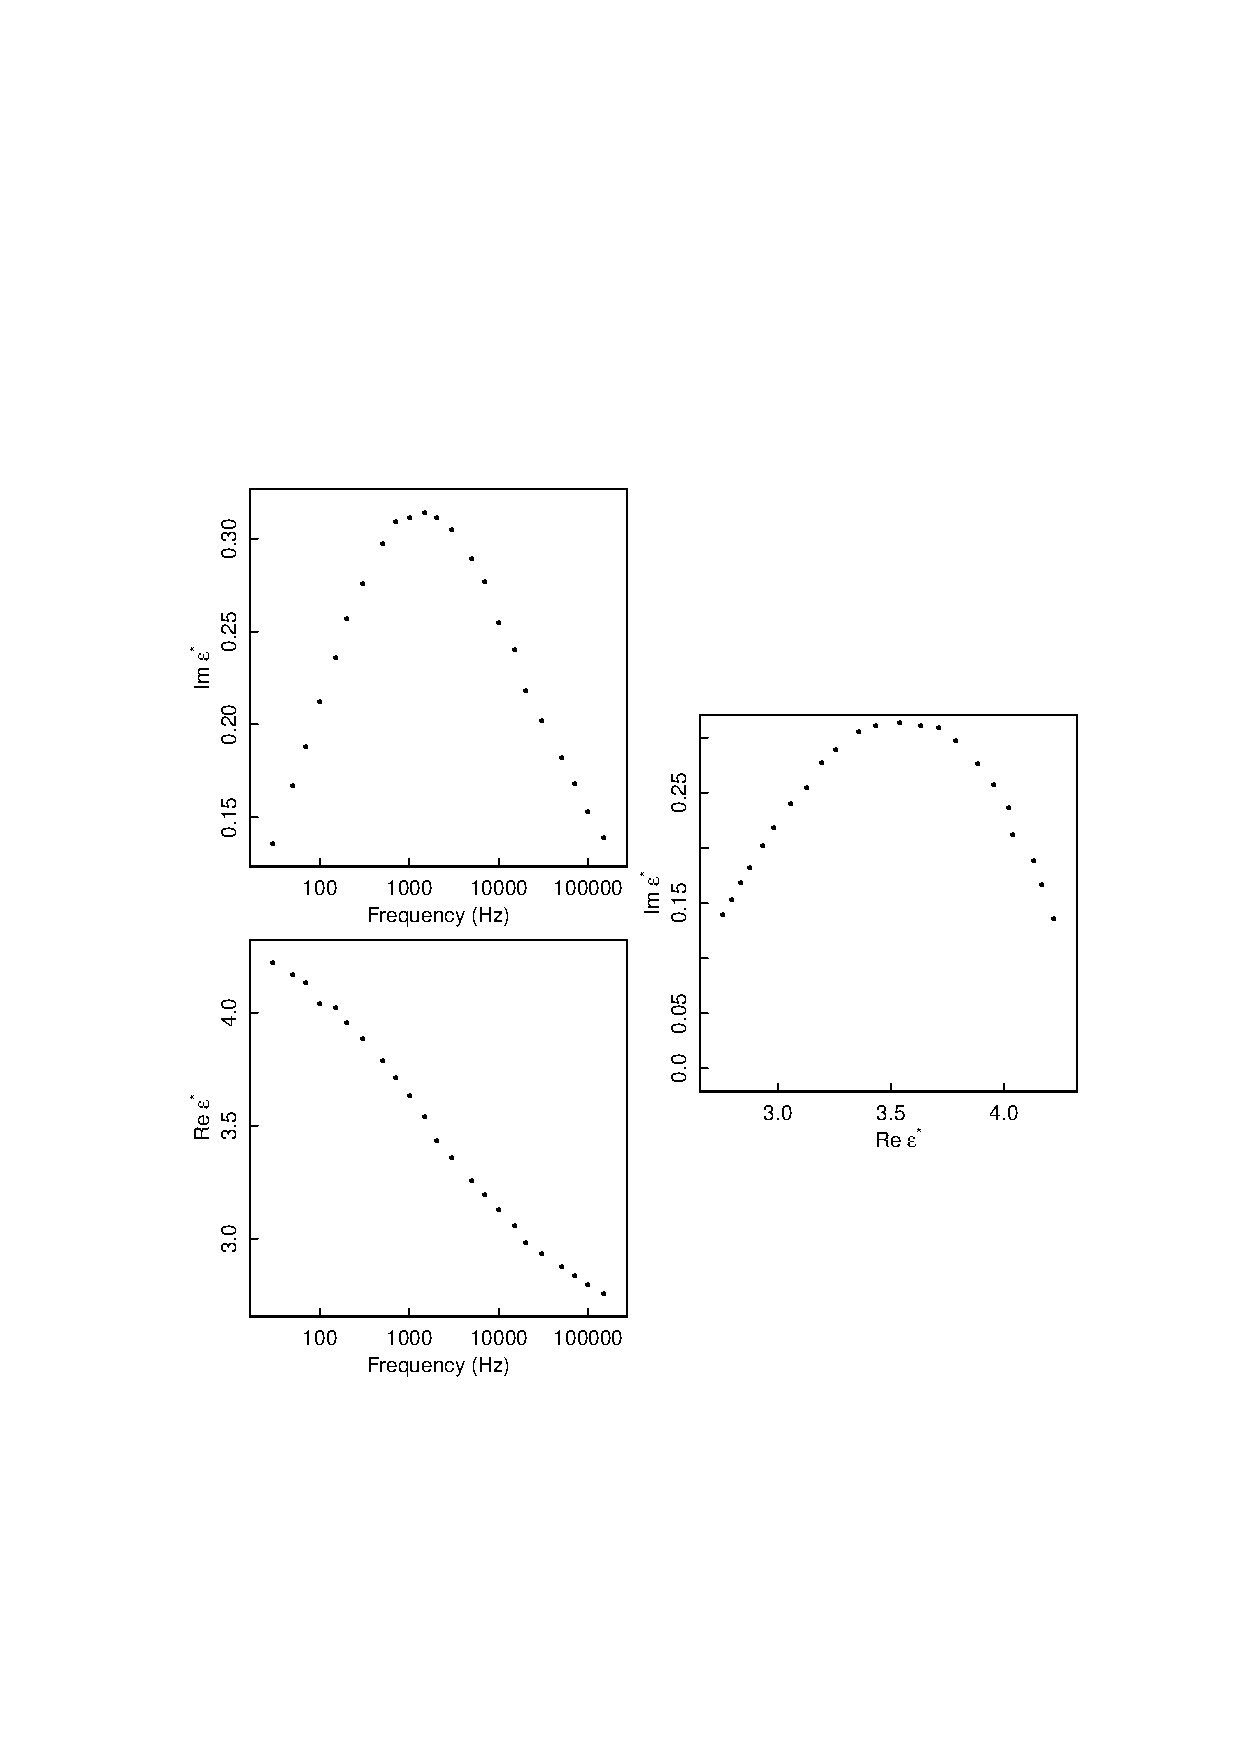
\includegraphics{4PMMAdata}}%,height=4in}}
    \caption{\label{fig:PMMAdata}
    Plots of the real and imaginary components of the dielectric constant
    $\epsilon^{*}$ (dimensionless)
    versus frequency (on a logarithmic scale) and in the complex
    plane for the s-PMMA dielectric data.
    }
  \end{figure}
$y_{\mbox{\it imag}}$ and the real component
$y_{\mbox{\it real}}$, versus frequency for syndiotactic
poly(methylmethacrylate) (s-PMMA) at 86.7$^\circ$F,
and, as recommended in \citeasnoun{cole:cole:1941},
%\glossary{ Cole, K.S.}
%\glossary{ Cole, R.H.}
in Figure~\ref{fig:PMMAdata}$c$ we plot these components in the complex
plane.
In this example, there are $M = 2$ responses, $N = 23$ cases,
and $P = 5$ parameters.
The data are listed in Appendix A, Section~\ref{atbl:spmma}.
\end{example}

As with uniresponse parameter estimation discussed in the
previous chapters, in the analysis of experimental data we assume
that the $N$ experimental design variables $ \bx_n $,
$n = 1 ,\ldots, N$, are fixed and known, so we can form the
$N \times M$ observation matrix $\bY$ with $(n,m)$th element
\index{matrix!observation}
$y_{nm}$ and the $N \times M$ expected response matrix
\index{matrix!expected response}
$\bH ( \btheta )$ with $(n,m)$th element
$ f_m ( \bx_n , \btheta )$.
From $\bY$ and $\bH ( \btheta )$, we create the residual matrix
\index{residual!matrix}
\index{matrix!residual}
\begin{equation}\label{eqn:4.3}
  \bZ ( \btheta ) = \bY - \bH ( \btheta )
\end{equation}

The parameter estimates $\hat{\btheta}$ are given by the values of
$\btheta$ which optimize some criterion based on
$\bZ ( \btheta )$ in the same
way that the least squares estimates in uniresponse parameter
estimation minimize $\norm \bz ( \btheta ) \norm^{2}$.
The criterion will depend on assumptions about the disturbance.
\index{assumptions!disturbance}
\index{assumptions!multiresponse}
For example, if we make the stringent assumption that the
${\rm Z}_{nm}$ are normally distributed and
independent with the same variance $\sigma^{2}$, then least squares
is appropriate and we find $\hat{\btheta}$ which minimizes
the sum of squared residuals of all $NM$ responses.
That is, the estimation criterion would be to minimize
the {\em trace\/}
of $\bZ \trans \bZ$, ${\rm \tr} ( \bZ \trans \bZ )$.
\index{trace!criterion for multiresponse estimation}

The assumptions leading to the trace criterion may not be
realistic.
It could be reasonable to assume that the variances of different
measurements on the same response are constant, but not that the
variances of different responses are equal.
Furthermore, assuming independent disturbances for different
measurements in the same experimental run may not be justified.
For example, in chemical experiments where the concentrations of
a number of different chemical species are measured from the same
sample, if only the relative concentrations can be determined,
different measurements on the same sample may be correlated.
Similarly, for dielectric determinations, errors in the frequency
settings can induce errors in both components.

Following \citeasnoun{box:drap:1965}, the model used to describe the
%\glossary{ Box, G.E.P.}
%\glossary{ Draper, N.R.}
disturbance term is a normal distribution with
$$
\mbox{\rm E} [ {\rm Z}_{nm} ] = 0
$$
and
$$
\mbox{\rm E} [ {\rm Z}_{nm} {\rm Z}_{ri} ] = \left\{
\begin{array}{c l}
  \{\bSIGMA\}_{mi}&n=r\\
  0&n\ne r
\end{array}\right.
$$
where $\bSIGMA$ is a fixed $M \times M$ covariance matrix.
\index{covariance!matrix}
\index{matrix!covariance}
That is, we
assume that measurements from different experiments are
independent but measurements from the same experiment are correlated.
The joint probability density function
for the $N$ observations, conditional on
all the unknown parameters, is then
\begin{eqnarray}\label{eqn:4.4}
  p(\bY|\btheta,\bSIGMA)&\sim&
  | \bSIGMA |^{- N/2}
  \exp\left[-{\tr[(\bY-\bH)\bSIGMA^{-1}(\bY-\bH)\trans]\over 2}\right]\\
  &=& | \bSIGMA^{-1} |^{N/2} \exp
  \left[ -{\tr ( \bZ \bSIGMA^{-1} \bZ \trans ) \over 2 }\right]\nonumber
\end{eqnarray}
where the vertical bars denote a determinant.

\subsection{The Determinant Criterion}
\index{determinant!criterion for multiresponse estimation}

A parameter estimation criterion under these assumptions can be
derived using a likelihood or Bayesian argument.
The loglikelihood function for the parameters $\btheta$ and
$\bSIGMA^{-1}$ is
\begin{equation}\label{eqn:4.5}
  L ( \btheta ,  \bSIGMA^{-1} ) = k + {N \over 2 }\ln | \bSIGMA^{-1} |-
  {\tr ( \bZ\bSIGMA^{-1} \bZ \trans ) \over 2 }
\end{equation}
where $k$ is an unimportant constant.
To maximize the loglikelihood function we write the last term as
${\rm \tr} ( \bZ \trans \bZ \bSIGMA^{-1} )$ and
differentiate the entire expression with
respect to the elements $\sigma^{mi}$ of $\bSIGMA^{-1}$.
Using the result \cite[p.~296]{bard:1974}
%\glossary{ Bard, Y.}
\begin{equation}\label{eqn:4.6}
  {\partial \ln | \bSIGMA^{-1} | \over \partial \sigma^{mi}}=
  \lb \bSIGMA \rb_{mi}
\end{equation}
allows us to write
$$
{\partial L ( \btheta , \bSIGMA^{-1} ) \over \partial \sigma^{mi}}=
{N \over 2 }\{\bSIGMA\}_{mi}{-1\over 2}\{\bZ\trans\bZ\}_{mi}
$$
Setting this derivative to zero provides the conditional estimates
$$
\lb \hat{\bSIGMA}( \btheta ) \rb_{mi}={\lb \bZ \trans \bZ \rb_{mi} \over N }$$
or
$$
\hat{\bSIGMA}( \btheta )={\bZ \trans \bZ \over N }$$
which, when substituted into (\ref{eqn:4.5}), gives the conditional loglikelihood
\index{loglikelihood!conditional}
function
\begin{equation}\label{eqn:4.7}
  L ( \btheta ,  \hat{\bSIGMA}( \btheta ) ) =
  k' - {N \over 2 }\ln | \bZ \trans \bZ |
\end{equation}
The maximum likelihood estimates are then obtained
\index{maximum likelihood estimate}
by minimizing $| \bZ \trans \bZ |$ with respect to $\btheta$.

A Bayesian argument was used by
\citeasnoun{box:drap:1965} to derive
%\glossary{ Box, G.E.P.}
%\glossary{ Draper, N.R.}
the marginal posterior density for $\btheta$ by integrating over
the unknown variances and covariances after incorporating an
noninformative prior of the form
$$
p ( \bSIGMA ,  \btheta ) \sim
| \bSIGMA |^{ - ( M + 1 ) /2 }
$$
The marginal posterior density is then
\begin{equation}\label{eqn:4.8}
  p ( \btheta | \bY ) \sim | \bZ \trans \bZ |^{{-} N/2}
\end{equation}
and so the posterior density is maximized when the determinant is
minimized.
Thus, the likelihood and Bayesian approaches lead to the same
criterion.

As pointed out in \citeasnoun{box:tiao:1973},
%\glossary{ Box, G.E.P.}
%\glossary{ Tiao, G.C.}
(\ref{eqn:4.7}) and (\ref{eqn:4.8}) are
remarkably general results, since they do not depend on whether
the expectation functions are linear or nonlinear, whether the
parameters are common to more than one response, or whether the
design variables are common to more than one response.
Furthermore, a scale change on any of the responses will not
affect the estimates, and linear combinations of the responses
can be used in place of the original responses.

Geometrically, $| \bZ \trans \bZ |$ corresponds to the square of the
\index{geometry!of multiresponse determinant criterion}
volume of the $M$-dimensional parallelepiped spanned by the residual
vectors,
\index{residual!vector}
$\bz_m ,m=1 ,\ldots, M$,
in the $N$-dimensional case space.
Minimizing the determinant corresponds to minimizing the volume
enclosed by the residual vectors.

\subsection{Inferences for Multiresponse Estimation}
\index{inference!in multiresponse estimation}

To draw inferences about parameters in multiresponse estimation,
we use the Bayesian formulation and
assume that $| \bZ \trans \bZ |$ can be
adequately represented by a quadratic Taylor series near
$\hat{\btheta}$ to give an approximate marginal posterior density function.
From (\ref{eqn:4.8}),
\begin{equation}\label{eqn:4.9}
  p(\btheta|\bY)\approx\left[{1+(\btheta-\hat{\btheta})\trans
  { { \bOMEGA   \over  2 | \hat{\bZ}\trans \hat{\bZ}| } }
  ( \btheta - \hat{\btheta}) }\right]^{{-}N/2}
\end{equation}
where $\bOMEGA$ is the Hessian of the determinant evaluated at
\index{Hessian!of determinant}
$\hat{\btheta}$.
This approximation has the form of a
$P$-variate Student's T density with location parameter
\index{T distribution!multivariate}
$\hat \btheta$, degrees of freedom $N-P$, scale factor
\begin{equation}\label{eqn:4.101}
  s^2 = {| \hat{\bZ}\trans \hat{\bZ}|} / (N - P)
\end{equation}
and covariance matrix
$2 s^2 \bOMEGA^{-1}$ \cite{box:tiao:1973}.
%\glossary{ Box, G.E.P.}
%\glossary{ Tiao, G.C.}
An approximate $1 - \alpha $ HPD region for
\index{highest posterior density (HPD)!approximate region in multiresponse estimation}
the parameters is given by
\begin{equation}\label{eqn:4.10}
  ( \btheta - \hat \btheta ) \trans
  {\bOMEGA  \over 2 }( \btheta - \hat \btheta )  \le 
  P s^2 \FPNP
\end{equation}
so that the square of the volume in the parameter space enclosed by
the joint region is proportional to the determinant of the Hessian.

Because we are approximating $| \bZ \trans \bZ |$, the
approximations (\ref{eqn:4.9}) and (\ref{eqn:4.10}) may be very poor:
additional research needs to be done to assess the adequacy of
these approximations even for cases where the model functions
are linear.
More accurate HPD regions can be written as either
\begin{equation}\label{eqn:Fregion}
  {( | \bZ \trans \bZ |-| \hat \bZ \trans \hat \bZ | ) / P \over s^2 }\FPNP
\end{equation}
or
\begin{equation}\label{eqn:Chiregion}
  \ln [p ( \hat \btheta | \bY ) ] - \ln [p ( \btheta | \bY ) ] 
  {1 \over 2 }\chi^2 ( P ; \alpha )
\end{equation}
\cite{box:tiao:1973}, where $\chi^2 ( P ; \alpha )$ is the upper
%\glossary{ Box, G.E.P.}
%\glossary{ Tiao, G.C.}
$\alpha$ percentile of the $\chi^{2}$ distribution with $P$
degrees of freedom.
Such regions would have to be determined numerically and
displayed in contour plots, and therefore suffer from the
disadvantages inherent in exact confidence and likelihood
regions for uniresponse models, as discussed in Chapter 6.
Nevertheless, the methods of Chapter 6 (profile $t$ and profile trace
plots) can be used for multiresponse problems.

An approximate $1 - \alpha $ HPD interval for the
\index{highest posterior density (HPD)!approximate interval in multiresponse estimation}
parameter $\theta_{p}$ is given by
\begin{equation}\label{eqn:4.12}
  \hat \theta_p\pm\tNP s \sqrt{2 \lb \bOMEGA^{-1} \rb_{pp}}
\end{equation}
and an approximate $1 - \alpha $ HPD band for the
\index{highest posterior density (HPD)!approximate band in multiresponse estimation}
$m$th expectation function $f_m ( \bx , \btheta )$ is
$$
f_m(\bx,\hat \btheta )\pm s\sqrt{2\bv_m \trans\bOMEGA^{-1} \bv_m}
\sqrt{P\FPNP}
$$
where $\bv_{m}$ is the gradient of $f_{m}$
with respect to $\btheta$ evaluated at $\bx$ and $\hat{\btheta}$.

\subsection{Dimensional Considerations in Multiresponse Estimation}

Note that the determinant criterion implies two important
constraints on the
\index{determinant!constraints for multiresponse estimation}
\index{constraint!in multiresponse estimation}
number of observations, $N$, the number of responses, $M$, and
the number of parameters, $P$.

First, $M$ can not exceed $N$, since otherwise the determinant is
identically zero.
To see this, note that the rank of the $N \times M$ matrix $\bZ$
cannot exceed the minimum of $( N , M )$, and when $NM$ the
rank of the $M \times M$ matrix $\bZ \trans \bZ$ is less than $M$ and
hence the determinant is identically zero.
Another way of seeing this is to recall from the geometric interpretation
that $| \bZ \trans \bZ |$
gives the square of the volume, in the $N$-dimensional case space,
enclosed by the residual vectors (columns of $\bZ$).
If the case dimension $N$ does not at least equal the
response dimension $M$, then the volume is zero.
For example, the volume of a rectangle is zero.

Second, in general $P$ must be less than $N$,
since otherwise the criterion
can be made zero by fitting any one response perfectly, or even by
fitting a linear combination of the responses perfectly.
That is, if there is an $M$-vector $\bv$ such that
$\bZ(\btheta)\bv=\boldsymbol{0}$ for some $\btheta$, then the determinant will
be zero at that value of $\btheta$ regardless of how well the
remaining responses have been fitted.

The reasoning leading to the constraint $N>P$ provides
justification for the use of $N-P$ for the residual degrees of
freedom proposed above.
It would seem that with $NM$ data values there
should be $N M - P$ degrees
of freedom for the residuals, as suggested in
\citeasnoun{bard:1974}, but in fact, near the
%\glossary{ Bard, Y.}
optimum the value of the determinant is controlled by the linear
combination of responses corresponding to the smallest singular
value of $\bZ$, and this vector has dimension $N$.
The vector corresponding to this singular value
therefore has $N - P$ degrees of freedom.

In summary, the number of cases, $N$, should exceed the maximum of $M$
and $P$ to ensure a successful analysis.

A great advantage in using multiresponse data is the increased
\index{multiresponse estimation!advantages and disadvantages}
precision of parameter estimates relative to those obtained from
uniresponse data.
However, we cannot attribute this increased precision to additional
denominator degrees of freedom when multiple responses are used.
The increased precision is due to the combination of different
types of information from the responses.

One difficulty with the use of multiresponse data is that
all problems become nonlinear optimization problems.
That is, even if the expectation functions are linear in the parameters,
iterative methods must be used to obtain the estimates which minimize
the determinant criterion.
The problem of obtaining the best estimates is also more difficult
than in the uniresponse nonlinear case, since the Hessian need not
be positive definite.
Further discussion on these aspects of optimizing the determinant
is given in Section 4.2.3.

Another difficulty with multiresponse estimation is that
inference regions for the parameters based on (\ref{eqn:4.10})
or (\ref{eqn:4.12}) are only approximate, even when all the
expectation functions are linear in the parameters.
The accuracy of these approximations is questionable.
On the other hand, inference regions from multiresponse
estimation are usually much smaller than those from uniresponse
estimation, and so approximate multiresponse regions may in fact
be better than approximate uniresponse regions for nonlinear models.

In spite of the difficulties,
multiresponse estimation is a valuable
technique and should be used whenever multiresponse data are available.
The reduction in size of the parameter inference regions,
together with the extra ability to discriminate between rival models,
is well worth any additional effort required.

\section{A Generalized Gauss--Newton Method}

One advantage of least squares as a criterion is that
specialized methods can be used to exploit properties of the
criterion and to provide standard optimization algorithms.
In this section, we describe a Gauss--Newton method for minimizing the
determinant criterion.

To evaluate the determinant, following \citeasnoun{bate:watt:1987},
%\glossary{ Bates, D.M.}
%\glossary{ Watts, D.G.}
\index{determinant!evaluation by QR decomposition}
we take a {\it QR} decomposition of $\bZ ( \btheta )$,
\index{QR decomposition!of residual matrix}
$$
\bZ ( \btheta ) = \bQ \bR = \bQ_1 \bR_1
$$
Then, since
\begin{eqnarray*}
  | \bZ ( \btheta ) \trans  \bZ ( \btheta ) |&=&| \bR_1 \trans \bR_1 |\\
  &=&| \bR_1 |^2\\
  &=&\prod_{m=1}^M\{\bR_1\}_{mm}^2
\end{eqnarray*}
we have  an  easy  way  to  evaluate  the  determinant
criterion for any  $\btheta$.

\subsection{The Gradient and Hessian of the Determinant}

The decomposition of $\bZ ( \btheta )$ as $\bQ_1 \bR_1 $ is
also helpful in evaluating the gradient and Hessian of the
determinant criterion.
To simplify notation we omit the dependence on
$\btheta$ and use a subscript enclosed in parentheses to
denote differentiation, as
$$
{ \partial \bZ   \over  \partial \theta_p } = \bZ_{(p)}
$$
Using the result (1.1.34) from \citeasnoun{fedo:1972},
%\glossary{ Fedorov, V.V.}
we have
\begin{equation}\label{eqn:4.14}
  {\partial | \bZ \trans \bZ |  \over \partial \theta_p } =
  | \bZ \trans \bZ |  \tr \left[ ( \bZ \trans \bZ )^{-1}
  {\partial ( \bZ \trans \bZ )  \over \partial \theta_p }
  \right]
\end{equation}
with
\begin{equation}\label{eqn:4.15}
  { \partial ( \bZ \trans \bZ )   \over  \partial \theta_p } =
  \bZ \trans \bZ_{(p)} + \bZ_{(p)} \trans \bZ
\end{equation}
so the gradient
\index{gradient!of determinant}
\index{determinant!gradient of}
$\bomega = \partial | \bZ \trans \bZ | / \partial \btheta \trans$
has components
\begin{eqnarray}\label{eqn:4.16}
  \lb \bomega \rb_p
  &=&2 | \bZ \trans \bZ |   \tr [ ( \bZ \trans \bZ )^{-1} \bZ \trans \bZ_{(p)} ]\\
  &=& 2 | \bZ \trans \bZ | \tr [ \bR_1^{-1} \bR_1 \invtrans
  \bR_1 \trans \bQ_1 \trans \bZ_{(p)} ]\nonumber\\
  &=& 2 | \bZ \trans \bZ |  \tr [ \bR_1^{-1} \bQ_1 \trans \bZ_{(p)} ]\nonumber\\
  &=& 2 | \bZ \trans \bZ |  \tr [ \bZ^+ \bZ_{(p)} ]\nonumber
\end{eqnarray}
where $\bZ^+ = \bR_1^{-1} \bQ_1 \trans$ is the
pseudoinverse of $\bZ$.

To obtain the second derivative or Hessian terms, we write
\index{Hessian!of determinant}
\index{determinant!Hessian of}
\begin{equation}\label{eqn:4.17}
  g = \ln | \bZ \trans \bZ |
\end{equation}
so that
\begin{equation}\label{eqn:4.17a}
  | \bZ \trans \bZ | = e^g
\end{equation}
and
\begin{equation}\label{eqn:4.18}
  g_{(p)} = 2  \tr [ \bZ^+ \bZ_{(p)} ]
\end{equation}
and then use the expressions for the derivative of the pseudoinverse
\cite{golu:pere:1973} to obtain
%\glossary{ Golub, G.H.}
%\glossary{ Pereyra, V.}
\begin{eqnarray}\label{eqn:4.19}
  g_{(pq)}&=&
  2 \lb - \tr [ \bZ^+ \bZ_{(p)} \bZ^+ \bZ_{(q)} ] +
  \tr [ \bZ^+ ( \bZ^+ ) \trans \bZ_{(p)} \trans
  ( \bI - \bZ \bZ^+ ) \bZ_{(q)} ]\\
  &&+\tr [ \bZ^+ \bZ_{(pq)} ] \rb\nonumber
\end{eqnarray}
From (\ref{eqn:4.17a}), a second derivative term for
$| \bZ \trans \bZ |$ is then
\begin{equation}\label{eqn:omega}
  {\partial^2 | \bZ \trans \bZ |  \over \partial \theta_p \partial \theta_q} =
  | \bZ \trans \bZ | [ g_{(p)} g_{(q)} + g_{(pq)} ]
\end{equation}

Alternative expressions for the gradient and Hessian of
$| \bZ \trans \bZ |$ are obtained by expanding (\ref{eqn:4.16}) as
\begin{eqnarray}\label{eqn:4.21}
  \lb \bomega \rb_p&=&
  | \bZ \trans \bZ | \tr [ ( \bZ \trans \bZ )^{-1}
  ( \bZ \trans \bZ_{(p)}+\bZ_{(p)} \trans \bZ ) ]\\
  &=&| \bZ \trans \bZ | \tr [ \bU_p ]\nonumber
\end{eqnarray}
where
$\bU_p = ( \bZ \trans \bZ )^{-1}
( \bZ \trans \bZ_{(p)} + \bZ_{(p)} \trans \bZ ) $.
Differentiating (\ref{eqn:4.21}) with respect to $\theta_{q}$ gives
\begin{eqnarray}\label{eqn:4.22}
  {\partial^2 | \bZ \trans \bZ | \over \partial \theta_q \partial \theta_p }&=&
  \lb \bomega \rb_q \tr [ \bU_p ]+| \bZ \trans \bZ | \lb
  - \tr [ \bU_q \bU_p ] +
  \tr [ ( \bZ \trans \bZ )^{-1}
  ( \bZ_{(q)} \trans \bZ_{(p)} + \bZ_{(p)} \trans \bZ_{(q)} ) ]\\
  &&+\tr [ ( \bZ \trans \bZ )^{-1}
  ( \bZ \trans \bZ_{(pq)}+\bZ_{(pq)} \trans \bZ ) ] \rb\nonumber\\
  &=&| \bZ \trans \bZ | \lb \tr [ \bU_q ] \tr [ \bU_p ]-
  \tr [ \bU_q \bU_p ]+
  \tr [ ( \bZ \trans \bZ )^{-1}
  ( \bZ_{(q)} \trans \bZ_{(p)}+\bZ_{(p)} \trans \bZ_{(q)} ) ]\nonumber\\
  &&+
  \tr [ ( \bZ \trans \bZ )^{-1}
  ( \bZ \trans \bZ_{(pq)}+\bZ_{(pq)} \trans \bZ ) ] \rb\nonumber\\
\end{eqnarray}

\subsection{An Approximate Hessian}
\index{Hessian!approximate}

The last term in the expression for $g_{(pq)}$
requires second derivatives of the model functions.
We prefer to avoid calculating second derivatives, especially
since the Hessian matrix is being used primarily to determine an
increment, and so we make the same assumption as in the
Gauss--Newton method for nonlinear least squares.
That is, we assume that the model functions can be locally
approximated by linear functions and set
$\bZ_{(pq)} $ to zero.
The {\em approximate Hessian\/} matrix $\bOMEGA$ is therefore
calculated with entries
\begin{eqnarray}\label{eqn:4.20a}
  \lb \bOMEGA \rb_{pq}&=&4 | \bZ \trans \bZ |
  \tr [ \bZ^+ \bZ_{(p)} ]\tr [ \bZ^+ \bZ_{(q)} ]\\
  &&+2 | \bZ \trans \bZ | \lb - \tr [ \bZ^+ \bZ_{(p)}
  \bZ^+ \bZ_{(q)} ]
  +\tr [ \bZ^+ ( \bZ^+ ) \trans \bZ_{(p)} \trans
  ( \bI-\bZ \bZ^+ ) \bZ_{(q)} ] \rb\nonumber\\
\end{eqnarray}
These can be collected into $\bOMEGA$ and used with the gradient vector
$\bomega$ to form the increment $\bdelta=- \bOMEGA^{-1} \bomega$ in a
Newton--Raphson iterative scheme to optimize $| \bZ \trans \bZ |$.
Since only first derivatives of the model functions
are used, this is a generalization
of the Gauss--Newton method for nonlinear least squares.
\index{Gauss--Newton!method for multiresponse estimation}

Some rearrangement of the terms in (\ref{eqn:4.16}) and
(\ref{eqn:4.19}) can be used
to simplify the calculations of $\bomega$ and $\bOMEGA$
\cite{bate:watt:1984}.
%\glossary{ Bates, D.M.}
%\glossary{ Watts, D.G.}
In particular, we can use the relationship
$\tr ( \bA \bB ) = \tr ( \bB \bA )$ to change (\ref{eqn:4.16}) to
\begin{eqnarray}\label{eqn:4.24}
  \lb \bomega \rb_p&=&
  2 | \bZ \trans \bZ |\tr [ \bQ_1 \trans \bZ_{(p)} \bR_1^{-1} ]\\
 &=&2 | \bZ \trans \bZ | \sum_{m=1}^M { g_{p,mm} }\nonumber
\end{eqnarray}
where $g_{p,mm}$ is the $(m,m)$th element of the
$N \times M$ matrix
\begin{equation}\label{eqn:4.24a}
  \bG_p = \bQ \trans \bZ_{(p)} \bR_1^{-1}
\end{equation}
This does not change the gradient calculation substantially, but
now (\ref{eqn:4.20a}) can be rewritten to give
\begin{eqnarray}\label{eqn:4.25}
  \lb \bOMEGA \rb_{pq}&=&4 | \bZ \trans \bZ | \sum_{m=1}^M
  { g_{p,mm} } \sum_{m=1}^M { g_{q,mm} }\\
  &&+2 | \bZ \trans \bZ | \lb - \tr [ \bQ_1 \trans \bZ_{(p)}
  \bR_1^{-1}  \bQ_1 \trans \bZ_{(q)} \bR_1^{-1} ]\nonumber\\
  &&+\tr [ \bR_1^{-1} \bQ_1 \trans \bQ_1
  \bR_1^{{{\rm }} -T}\bZ_{(p)} \trans \bQ_2 \bQ_2 \trans \bZ_{(q)} ]
  \rb\nonumber\\
  & = & 4 | \bZ \trans \bZ | \sum_{m=1}^M
  {g_{p,mm}}\sum_{m=1}^{M{g}_{q,mm}}\nonumber\\
  &&+ 2 | \bZ \trans \bZ | \left( - \sum_{m=1}^M
  \sum_{i=1}^M g_{p,mi} g_{q,im} +
  \tr [ ( \bQ_2 \trans \bZ_{(p)} \bR_1^{-1} ) \trans
  ( \bQ_2 \trans \bZ_{(q)} \bR_1^{-1} ) ] \right)\nonumber\\
  &=&4 | \bZ \trans \bZ | \sum_{m=1}^M
  g_{p,mm} \sum_{m=1}^M g_{q,mm}\nonumber\\
  &&+ 2 | \bZ \trans \bZ | \left( - \sum_{m=1}^M
  \sum_{i=1}^M {g_{p,mi} g_{q,im}} +
  \sum_{m=M+1}^N 
  \sum_{i=1}^M {g_{p,mi} g_{q,mi}} \right)
\end{eqnarray}
Equation (\ref{eqn:4.25}) permits very efficient evaluation of $\bOMEGA$,
because once the $QR$ decomposition of $\bZ$ is done and
the matrices $\bG_p ,  p = 1 ,\ldots, P$, are formed, it is only
necessary to collect a few inner products.
As discussed in Appendix 2, although $\bQ \trans$ occurs as a factor
in (\ref{eqn:4.24a}),
the matrix $\bQ$ is not explicitly formed; instead, a product
such as $\bQ \trans \bZ_{(p)} $ is formed by applying
Householder transformations to $\bZ_{(p)} $.

\subsection{Calculations for Each Iteration}

At each iteration, the current value of the parameter vector,
$\btheta^{0}$, is used to evaluate $| \bZ \trans \bZ |$, the gradient
$\bomega$, and the approximate Hessian $\bOMEGA$.
If $\bOMEGA$ is positive definite, the increment is calculated by
\index{Gauss--Newton!increment for multiresponse estimation}
solving
\begin{equation}\label{eqn:4.23a}
  \bOMEGA \bdelta^0 = - \bomega
\end{equation}
for $\bdelta^{0}$ and setting
$$
\btheta^1 =  \btheta^0 + \lambda \bdelta^0
$$
where $\lambda$ is a step size factor chosen to ensure that
\index{step factor}
$ | \bZ ( \btheta^1 ) \trans \bZ ( \btheta^1 ) | 
| \bZ ( \btheta^0 ) \trans \bZ ( \btheta^0 ) |$.
The solution to (\ref{eqn:4.23a}) is accomplished most efficiently by taking
a Cholesky decomposition of $\bOMEGA$ \cite[Chapter 8]{dong:bunc:mole:stew:1979} as
%\glossary{ Dongerra, J.J.}
%\glossary{ Bunch, J.R.}
%\glossary{ Moler, C.B.}
%\glossary{Stewart, G.W.}
\index{Cholesky!decomposition}
\begin{equation}\label{eqn:cholesky}
  \bOMEGA = \bC \trans \bC
\end{equation}
where $\bC$ is $P\times P$ and upper triangular.

Unlike the Gauss--Newton method for nonlinear least squares, the
generalized Gauss--Newton method for multiresponse data need not
result in a positive definite $\bOMEGA$.
\index{Hessian}
One of the situations in which negative eigenvalues of the Hessian can
occur is when there are multiple minima for the determinant criterion,
such as in the case study of Section 5.5.

When $\bOMEGA$ is not positive definite, the quadratic
approximation to $| \bZ \trans \bZ |$ does
not have a minimum and $\bC$ cannot
be calculated.
As in Section 3.5, we restore positive definiteness to the
Hessian by inflating the diagonal and
modifying the increment to be the solution of
$$
( \bOMEGA + k \bI ) \bdelta^0 = - \bomega
$$
where $k$ is large enough to make $\bOMEGA + k \bI$ positive
definite.
Such a $k$ can be calculated by determining the eigenvalues of
$\bOMEGA$ and setting $k$ to twice the magnitude of the most
negative eigenvalue, or by using a modified Cholesky
decomposition \citeasnoun{denn:schn:1983}.
%\glossary{ Dennis, J.E.Jr.}
%\glossary{ Schnabel, R.B.}

\subsection{A Multiresponse Convergence Criterion}
\index{multiresponse estimation!convergence criterion}

To decide whether we have convergence at a particular parameter
vector $\btheta^{0}$, we reason as in Section 2.2.3 and compare the
magnitude of the increment at that point with the statistical
variability in the estimates.
The statistical variability is accounted for in the elliptical regions
of (\ref{eqn:4.10}), and so we take a linear transformation of the
parameters to make the regions spherical.
With such a transformation, the length of the increment
from $\btheta^{0}$ is simply $\norm \bC \bdelta \norm$, where $\bC$ is the
Cholesky factor from (\ref{eqn:cholesky}), and the region is
simply a disk with radius proportional to
$s\sqrt{P\FPNP}$.
The convergence criterion is then \cite{bate:watt:1987}
%\glossary{ Bates, D.M.}
%\glossary{ Watts, D.G.}
\index{convergence!criterion for multiresponse estimation}
$$
{ \norm \bC \bdelta \norm^2 / P   \over  2 s^2 }  \epsilon^2
$$
where $\epsilon$ is the tolerance level and $s^{2}$ is the scale
factor (\ref{eqn:4.101}).
When the criterion is small, it indicates that the requested
increment is negligible relative to the statistical variability.
The value of $\epsilon$ can be set at 0.001, reasoning as in
Section 2.2.3.

Pseudocode for multiresponse parameter estimation is presented in
Appendix 3, Section A3.3.

\section{Practical Considerations}
\index{practical considerations!in multiresponse estimation}
\index{multiresponse estimation!practical considerations}

As in uniresponse estimation, care should be taken in selecting the
model and obtaining starting estimates for the parameters.
After convergence, residuals for all the responses should be
examined using plots as described in Chapter 3.
However, multiresponse modeling involves additional practical
considerations, as discussed below.

\subsection{Obtaining Starting Values}
\index{starting values!multiresponse}

The techniques for obtaining starting estimates for uniresponse
models described in Chapter 3 can be used for multiresponse
models by applying the procedures to each response and
then combining the estimates to give starting values for the complete
parameter vector.
Graphical analyses can be especially helpful, as illustrated in
the following example.

\begin{example}\label{spmma:graph}
Starting estimates for the parameters in the expectation
function for the complex dielectric coefficient can be obtained
from graphical considerations, following \citeasnoun{havr:nega:1967}.
%\glossary{ Havriliak, S.Jr.}
%\glossary{ Negami, S.}
They showed that the real and imaginary components can be written
  \begin{eqnarray*}
    \epsilon'&=&\epsilon_{\infty} +
    ( \epsilon_0 - \epsilon_{\infty} ) R^{ - \beta }  \cos\beta \phi\\
    \epsilon''&=&
( \epsilon_0 - \epsilon_{\infty} ) R^{{-} \beta}  \sin\beta \phi
  \end{eqnarray*}
where
$$
R^2 =
\left[ 1 + ( 2 \pi f / f_0 )^{\alpha}
\cos ( \pi \alpha / 2 )\right]^2
+ \left[ ( 2 \pi f / f_0 )^{\alpha}
\sin ( \pi \alpha / 2 )\right]^2
$$
and
$$
\phi = \arctan \left[
{ ( 2 \pi f / f_0 )^{\alpha}
\sin ( \pi \alpha / 2 )  
\over   1+( 2 \pi f / f_0 )^{\alpha}
\cos ( \pi \alpha / 2 ) }\right]
$$
The parameters $\epsilon_{0}$ and $\epsilon_{\infty}$ are the
limiting low and high frequency intercepts of the locus with the
real axis, when the function is plotted in the complex plane.
Furthermore, the limiting angle the high frequency locus makes
with the real axis is
$ \psi_L = \pi \alpha \beta / 2 $, and the angle
bisector of $ \psi_L $ from $( \epsilon_{\infty} , 0 )$ intersects the
locus at the frequency $\tilde f $ for which
$2 \pi \tilde f / f_0 = 1$.
And finally, $\alpha$ is related to $ \psi_L $
through
$$
\psi_L = - \pi \alpha
{ \ln \left( \tilde {R \over  \epsilon_0 - \epsilon_{\infty} }\right)  
\over \ln[ 2+2\cos( \pi \alpha / 2 ) ]}
$$
where $\tilde R $ is the length of the line from
$( \epsilon_{\infty} , 0 )$ to $\epsilon * ( \tilde f ) $.

To obtain starting values for the s-PMMA data, we plotted the data
in the complex plane, as in Figure \ref{fig:PMMAdata}$c$, but this time we
made the scales of the real and imaginary parts equal so that angles and
distances would be correct.
We extrapolated the right hand portion of the curve to the real
axis to give the starting value $\epsilon_0^0 = 4.40$, and
extrapolated the left hand portion to the real
axis to give the starting value $\epsilon_{\infty}^0 = 2.36$.
Next, we measured the angle of the left hand extrapolation line to the
real axis to give the limiting angle estimate $\psi_L = 19^\circ$.
The bisector of this angle intercepts the data between the points
corresponding to 200 and 300 Hz, so we took the value of
$(\ln f_0 )^{0}=\ln[ 2 \pi ( 250 )]=7.36$.
The length $\tilde R$ was measured to be 1.6, and
using this value together with that of the limiting angle, we solved for
$\alpha^0 = 0.53$ and, finally, $\beta^0 = 0.40$.
\end{example}

\subsubsection{Starting Estimates for Multiresponse Models Described by
Systems of Linear Differential Equations}
\index{starting values!systems of differential equations}

For multiresponse models described by systems of differential
equations, such as in Example $\alpha$-Pinene 1 or
$\alpha$-Pinene \ref{pin:model}, one can exploit the relation
between the rates and the responses to develop a simple procedure
for determining starting values
\cite{bate:watt:1985,vara:1982}.
%\glossary{ Bates, D.M.}
%\glossary{ Watts, D.G.}
%\glossary{ Varah, J.M.}
The general approach is to derive estimates for the rates and
then solve the simpler linear or nonlinear set of equations
rather than using numerical integration to solve the differential
equations.
In \citeasnoun{vara:1982}, cubic spline fits were made to the data and
%\glossary{ Varah, J.M.}
rates were obtained by differentiating the spline fits.
A cruder approach is to use simple differences to obtain
rate estimates, as was used in Example Ethyl acrylate 2, and
illustrated below for multiresponse data.
\label{pin:2}
\begin{example}

A linear kinetic model was proposed
in \citeasnoun{box:hunt:macg:erja:1973} for the
%\glossary{ Box, G.E.P.}
%\glossary{ Hunter, W.G.}
%\glossary{ MacGregor, J.M.}
%\glossary{ Erjavec, J.}
$\alpha$-pinene data, of the form
  \begin{eqnarray*}
    {d \gamma_1 \over dt}&=&-(\theta_1+\theta_2)\gamma_1\\
    {d \gamma_2 \over dt}&=&\theta_1 \gamma_1\\
    {d \gamma_3 \over dt}&=&\theta_2\gamma_1-(\theta_3+\theta_4)\gamma_3 +
    \theta_5 \gamma_5\\
    {d \gamma_4 \over dt}&=&\theta_3 \gamma_3\\
    {d \gamma_5 \over dt}&=&\theta_4 \gamma_3 - \theta_5 \gamma_5
  \end{eqnarray*}
The explicit solution to this set of linear differential
equations was given in \citeasnoun{box:hunt:macg:erja:1973}, and
%\glossary{ Box, G.E.P.}
%\glossary{ Hunter, W.G.}
%\glossary{ MacGregor, J.M.}
%\glossary{ Erjavec, J.}
involves long complicated expressions.

An alternative form is the matrix equation
$$
\left[  \matrix {
\matrix { \dot \gamma_1 \cr \dot \gamma_2 \cr \dot \gamma_3
\cr \dot \gamma_4 \cr \dot \gamma_5 } }\right] =
\left[ \matrix {
\matrix { - \theta_1 - \theta_2 \cr \theta_1 \cr \theta_2
\cr 0 \cr 0 }
\matrix { 0 \cr 0 \cr 0 \cr 0 \cr 0 }
\matrix { 0 \cr 0 \cr - \theta_3 - \theta_4 \cr
\theta_3 \cr \theta_4 }
\matrix { 0 \cr 0 \cr 0 \cr 0 \cr 0 }
\matrix { 0 \cr 0 \cr 0 \theta_5 \cr
0 \cr - \theta_5 } }\right]
\left[  \matrix {
\matrix { \gamma_1 \cr \gamma_2 \cr \gamma_3
\cr \gamma_4 \cr \gamma_5 } }\right]
$$
or
$$
\dot{\bgamma}= \bA \bgamma
$$
where $\bA$ is the system transfer matrix, and
\index{transfer matrix}
\index{matrix!system transfer}
a dot denotes differentiation with respect to time.
Further discussion of linear differential equation models
is given in Chapter 5.

To derive an expression useful for obtaining starting values,
we rewrite the matrix equation as
$$
\left[ \matrix {
\matrix { \dot \gamma_1 \cr \dot \gamma_2 \cr \dot \gamma_3
\cr \dot \gamma_4 \cr \dot \gamma_5 } }\right] =
\left[ \matrix {
\matrix { - \theta_1 \gamma_1 - \theta_2 \gamma_1
\cr \theta_1 \gamma_1
\cr \theta_2 \gamma_1 - \theta_3 \gamma_3 - \theta_4
 \gamma_3 + \theta_5 \gamma_5
\cr \theta_3 \gamma_3
\cr \theta_4 \gamma_3 - \theta_5 \gamma_5 } }\right] =
\bX ( t ) \btheta
$$
where
$$
\bX ( t ) = \left[ \matrix {
 \matrix{- \gamma_1 \cr \gamma_1 \cr 0 \cr 0 \cr 0}
 \matrix{- \gamma_1 \cr 0 \cr 0 \gamma_1 \cr 0 \cr 0}
 \matrix{ 0 \cr 0 \cr - \gamma_3 \cr \gamma_3 \cr 0}
 \matrix{ 0 \cr  0 \cr - \gamma_3 \cr  0 \cr \gamma_3}
 \matrix{ 0 \cr  0 \cr  \gamma_5 \cr  0 \cr - \gamma_5}
}\right]
$$

At any time $t$, therefore, if we have estimates for the rates and
the concentrations, we could estimate $\btheta$ by linear
regression of $\dot{\bgamma}$ on $\bX$.
Collecting the estimated rates for each time into
a vector gives the ``response''
vector for the linear regression.
Similarly, we calculate $\bX ( t )$ matrices for each time, using the
average concentrations, and
stack them to form the $\bX$ matrix.

For example, the estimated rates at $t=1230$ are
$$
( -9.47 , 5.93 , 1.87 , 0.33 , 1.43 ) \trans \times 10^{-3}
$$
and the average concentrations, inserted into the appropriate matrix, are
$$
\left[ \matrix {
\matrix { - 94.2 \cr 94.2 \cr 0 \cr 0 \cr 0 }
\matrix { - 94.2 \cr 0 \cr 94.2 \cr 0 \cr 0 }
\matrix { 0 \cr 0 \cr -1.15 \cr 1.15 \cr 0 }
\matrix { 0 \cr 0 \cr -1.15 \cr 0 \cr 1.15 }
\matrix { 0 \cr 0 \cr 0.88 \cr 0 \cr - 0.88 }
}\right]
$$
Finally, we stack the vectors from each time to form a single vector,
stack the matrices to form a single matrix, and then perform a simple
linear regression with no intercept term to get the starting
estimates.
The starting values so obtained are
$$
\btheta^0 = ( 5.84 ,  2.65 ,  1.63 ,  27.77 ,  4.61 ) \trans
\times 10^{-5}
$$
Because the parameters are rate constants, which are necessarily
positive, we fit the model in the parameters
$ \phi_p = \ln\theta_p $ (see Section 3.4.1).
\end{example}

When some of the responses are not measured, it is still possible
to use approximate rates provided other information, such as a
mass balance, is substituted.
In addition to providing starting values, the approximate rate
method provides useful information on the estimation situation,
and can even be used for parameter estimation \cite{vara:1982},
%\glossary{ Varah, J.M.}
although, when estimating parameters, one should ensure that the
implicit assumptions on the distribution of the noise terms are
reasonable.

\subsection{Assessing the Fit}
\index{multiresponse estimation!assessing fit}

As in any statistical analysis, it is extremely important to
assess the fit.
Generally, the best type of assessment involves plotting the
residuals for all responses versus the design variables, versus
\index{residual!plot}
each other, and versus the fitted responses, plus overlay plots
of the data and the fitted responses.
These plots are especially important in that they can reveal
whether the program has converged to a spurious optimum due to
dependencies in the data or in the residuals.

\begin{example}\label{spmma:3}
Convergence output for the s-PMMA data is given in
Table~\ref{tbl:4.2}.
\begin{table}
  \caption{\label{tbl:4.2}
  Parameter summary for the s-PMMA data
  }
  \begin{center}
    \begin{tabular}{clllllll}\hline
      \multicolumn{1}{c}{Parameter} & \multicolumn{1}{c}{Estimate} &
      \multicolumn{1}{c}{Approx.} & \multicolumn{5}{c}{Approximate}\\
      && \multicolumn{1}{c}{Std.Error} &
      \multicolumn{5}{c}{Correlation Matrix}\\ \hline
      $\epsilon_{0}$&4.320&0.011&1.00\\
      $\epsilon_{\infty}$&2.522&0.018&0.75&1.00\\
      $\ln f_{0}$&7.956&0.084&0.46&0.74&1.00\\
      $\alpha$&0.531&0.010&--\/0.57&--\/0.71&--\/0.93&1.00\\
      $\beta$&0.554&0.030&0.53&0.84&0.95&--\/0.95&1.00\\ \hline
    \end{tabular}
  \end{center}
\end{table}
The residuals for the real and imaginary components are
plotted versus frequency in
Figure~\ref{fig:PMMAres1}.
\begin{figure}
  \centerline{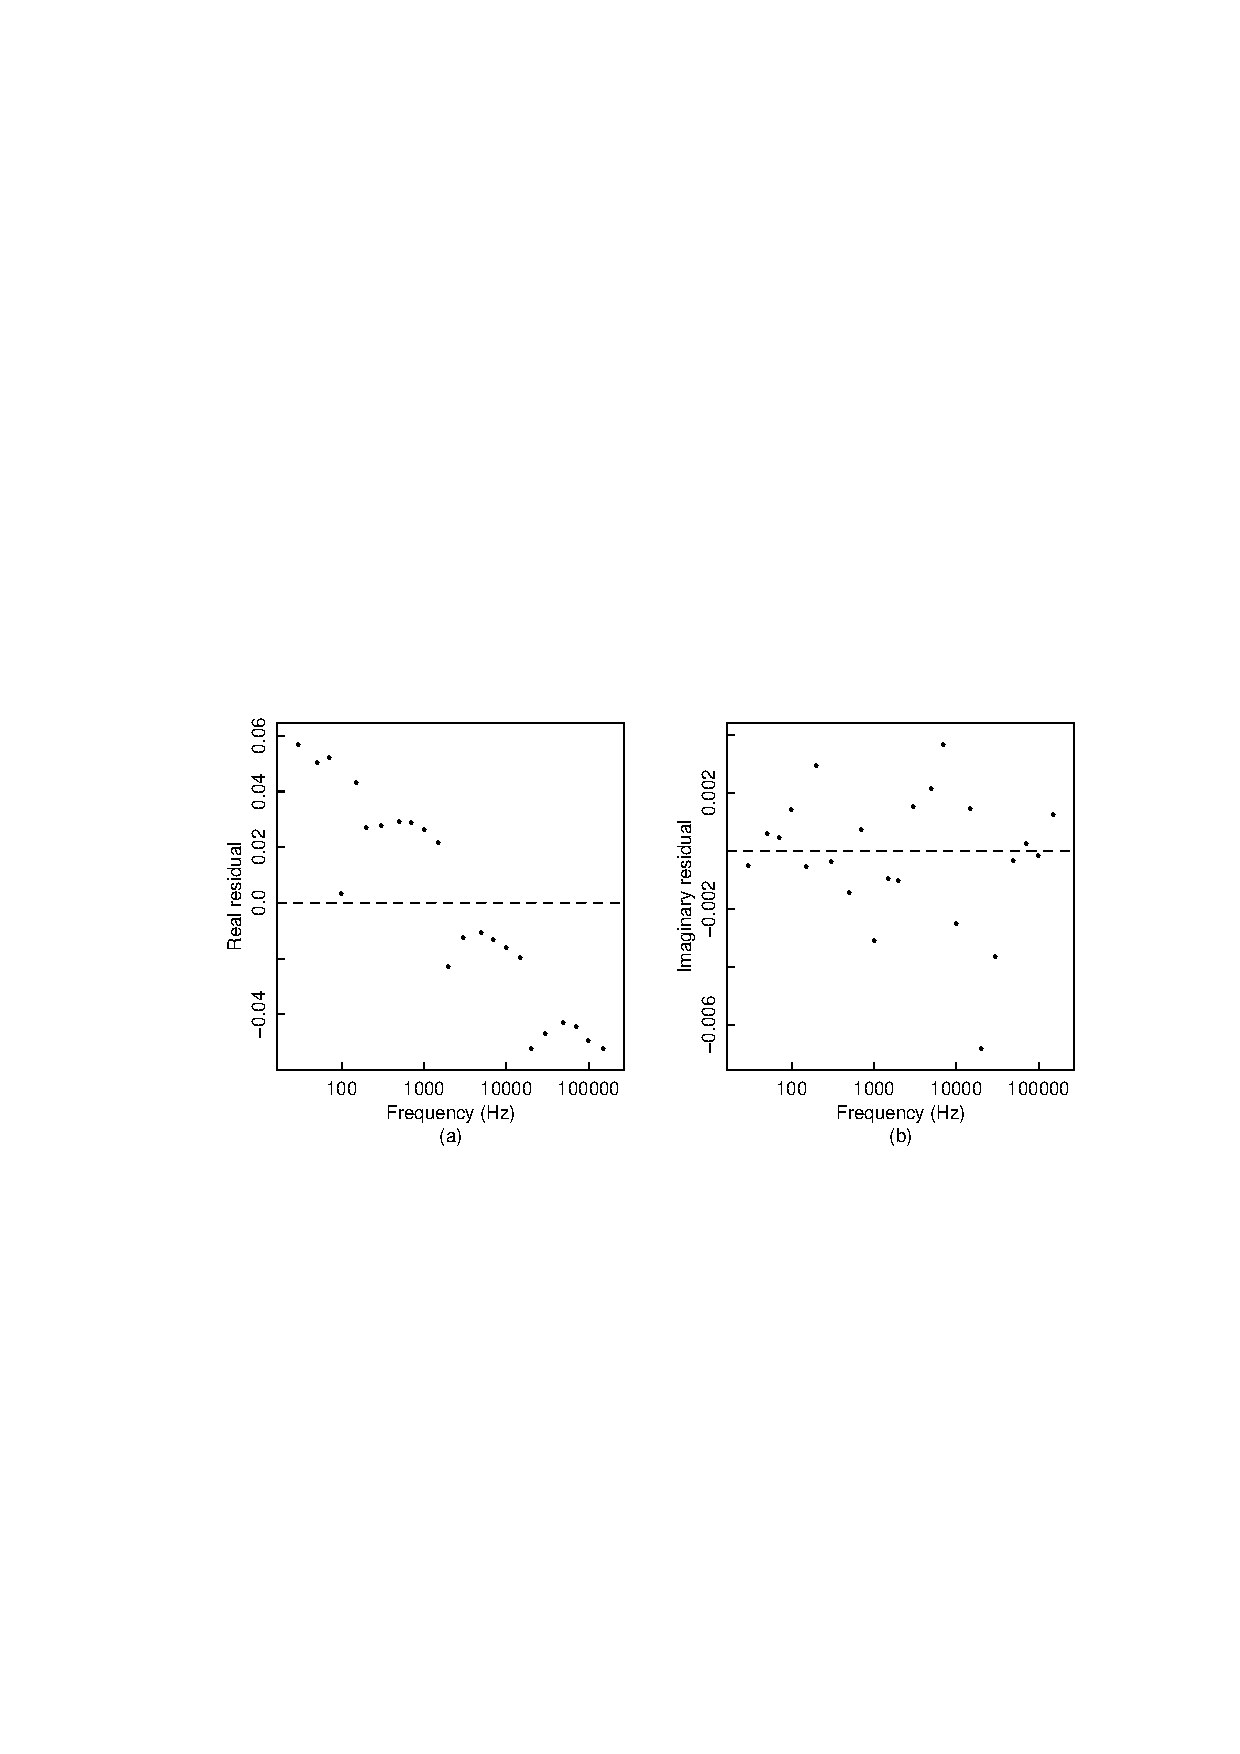
\includegraphics{4PMMAres1}}%,height=2.25in}}
  \caption{\label{fig:PMMAres1}
  Residuals from the initial fit to the s-PMMA data.
  }
\end{figure}
The imaginary residuals are quite well behaved, but the
real residuals are grouped and have a strong trend
with frequency.

As discussed in \citeasnoun{havr:watt:1987},
%\glossary{ Havriliak, S.Jr.}
%\glossary{ Watts, D.G.}
this behavior can be explained by considering the way in
which the frequencies are set in an experiment.
When the frequency of an oscillator is made to cover an
extremely large range (in this example, from 30 to
150000 Hz), it is done by manipulating two dials, a {\em units\/}
dial which covers a range of, say, 2 to 20,
and a {\em decade\/} dial which changes the frequency by
multiples of 10.
Thus, to set the frequency to 150 Hz, the
operator would set the units dial to 15 and the
decade dial to $\times 10$; and to set the frequency to 30000
Hz, the operator would set the units dial to 3 and the
decade dial to $\times 10000$.
In this experiment, the capacitance of
the polymer sample was apparently large enough to affect the
frequency of the oscillator, so that the actual frequency
delivered was not that indicated on the dials.
At high
frequencies the fitted values were too large, and at low
frequencies the fitted values were too small, suggesting
that the indicated frequencies were below the actual, with
the discrepancy (indicated -- actual) increasing with each decade
increase.

A decade correction was therefore made to the indicated
frequencies so that when the decade was increased, the
frequency was multiplied by $10\times K$.
Assuming the
first decade was correct, the second decade would have
actual frequencies of $K \times$ the indicated values, the
third decade $K^{2\times} $ the indicated values, and so
on.
Rather than incorporate the decade factor $K$ as a
parameter in the model, we performed a search by selecting
values for $K$, modifying the indicated frequencies,
fitting the model and examining the residuals, and choosing
that value of $K$ which gave the best behaved residuals.
For this data set, a decade correction of $K = 1.25 $ was
found.

The convergence output for the decade-corrected data is
given in
Table~\ref{tbl:4.3}.
\begin{table}
  \caption{\label{tbl:4.3}
  Parameter summary for the decade-corrected s-PMMA data
  }
  \begin{center}
    \begin{tabular}{cllrrrrr}\hline
      \multicolumn{1}{c}{Parameter} & \multicolumn{1}{c}{Estimate} &
      \multicolumn{1}{c}{Approx.} & \multicolumn{5}{c}{Approximate}\\
      && \multicolumn{1}{c}{Std.Error} &
      \multicolumn{5}{c}{Correlation Matrix}\\ \hline
      $\epsilon_{0}$&4.400&0.007&1.00\\
      $\epsilon_{\infty}$&2.447&0.013&0.58&1.00\\
      $\ln f_{0}$&8.228&0.091&0.68&0.84&1.00\\
      $\alpha$&0.486&0.008&--\/0.86&--\/0.68&--\/0.91&1.00\\
      $\beta$&0.571&0.026&0.76&0.85&0.99&--\/0.95&1.00\\ \hline
    \end{tabular}
  \end{center}
\end{table}
The major changes were a reduction in the determinant and in
the variance estimate of the real residuals by
a factor of about 10.
The residuals for the real and imaginary components are
plotted versus frequency in
Figure~\ref{fig:PMMAres2},
\begin{figure}
  \centerline{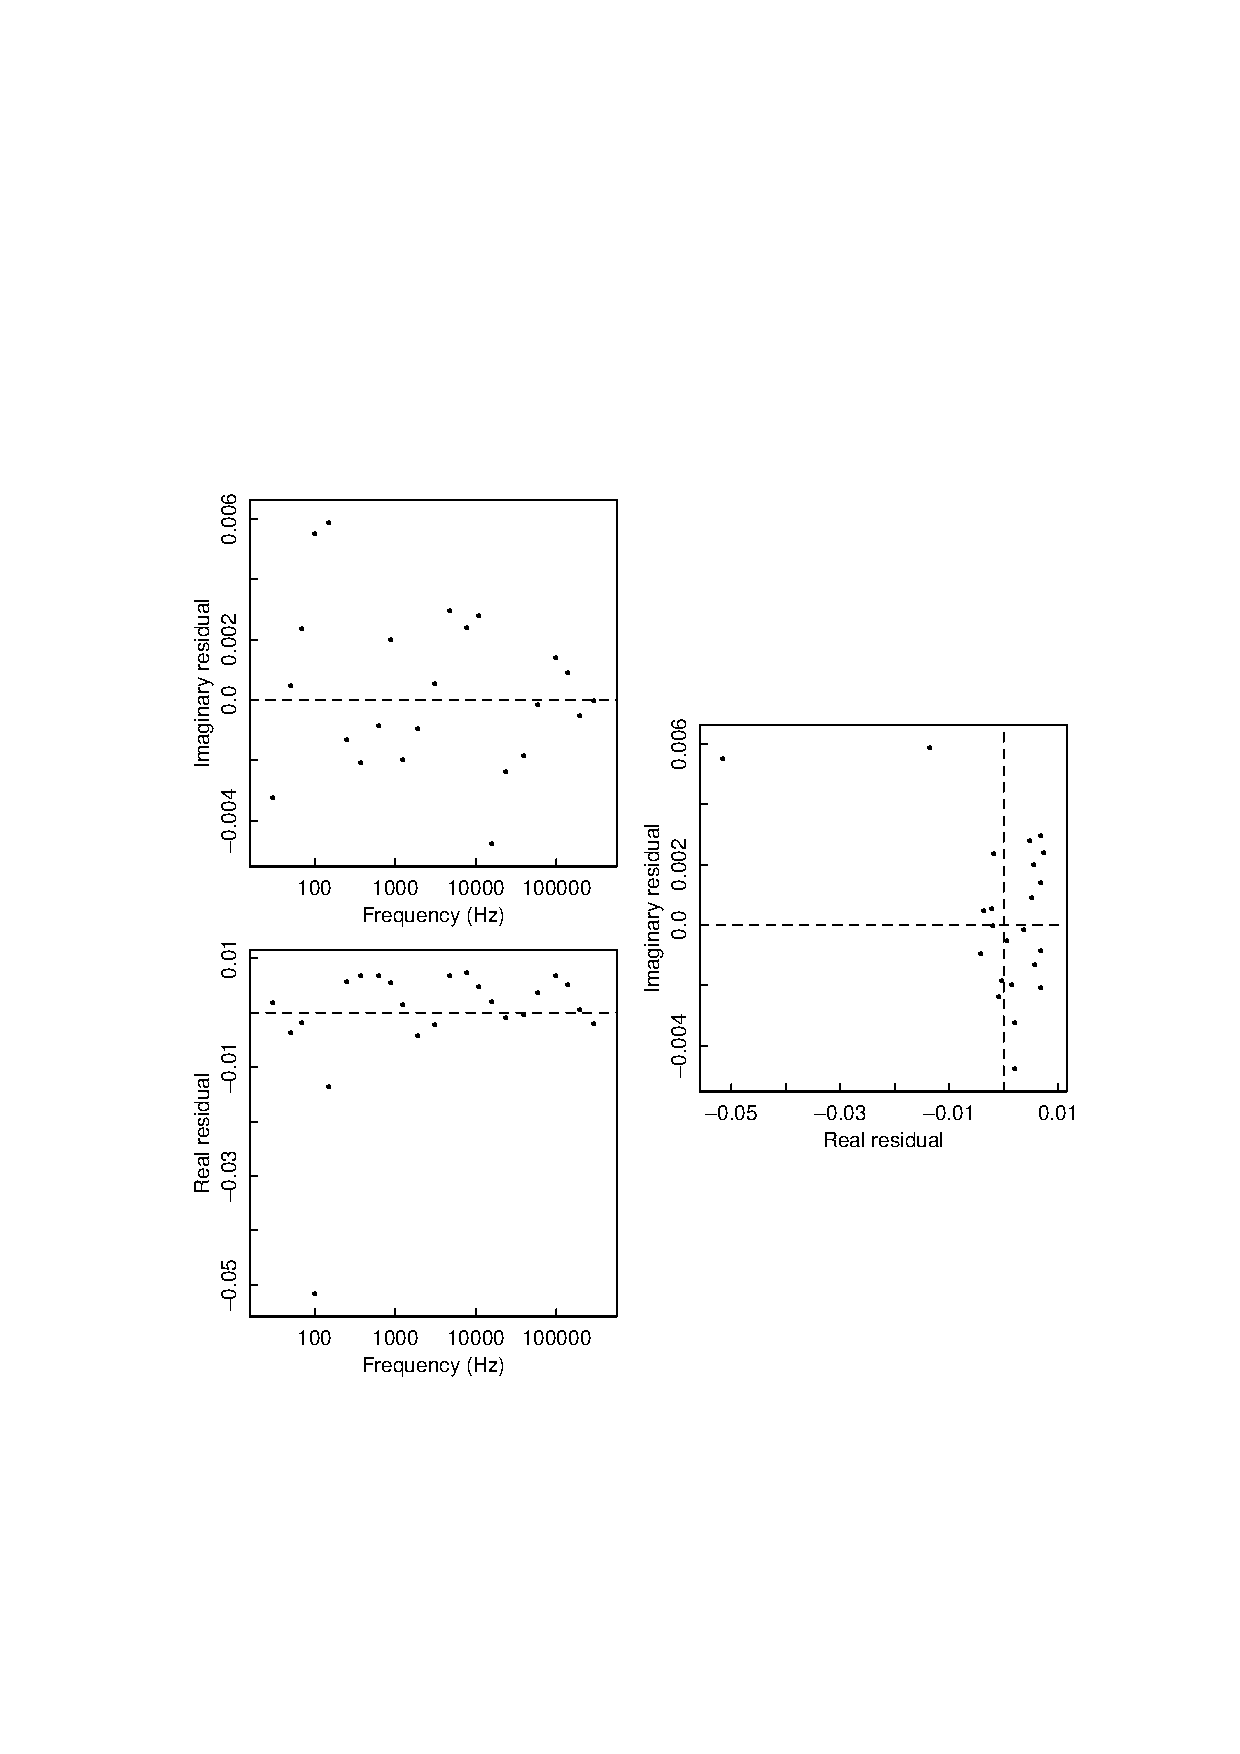
\includegraphics{4PMMAres2}}%,height=4.5in}}
  \caption{\label{fig:PMMAres2}
  Residuals from the fit to the decade-corrected s-PMMA data.
  }
\end{figure}
from which it can be seen that the imaginary residuals are
very well behaved, with perhaps two or three outliers.
The real residuals are much better behaved now, with no trend.
There is, however, one obvious outlier and one other
possible outlier.
Plotting the imaginary residuals versus the real residuals
more clearly discloses two outliers.
Since the residuals are bad in both the real and imaginary components,
we simply delete these two cases.
If only one residual were bad, we could treat the
observation which gave rise to the bad residual as missing, and
proceed as in Section 4.4.

Analysis of the decade-corrected and edited data set produced
the results in
Table~\ref{tbl:4.4}.
\begin{table}
  \caption{\label{tbl:4.4}
  Parameter summary for the decade-corrected and edited s-PMMA data}
  \begin{center}
    \begin{tabular}{cccrrrrr}\hline
      \multicolumn{1}{c}{Parameter} & \multicolumn{1}{c}{Estimate} &
      \multicolumn{1}{c}{Approx.} & \multicolumn{5}{c}{Approximate}\\
      && \multicolumn{1}{c}{Std.Error} &
      \multicolumn{5}{c}{Correlation Matrix}\\ \hline 
      $\epsilon_{0}$&4.398&0.006&1.00\\
      $\epsilon_{\infty}$&2.451&0.010&0.53&1.00\\
      $\ln f_{0}$&8.245&0.074&0.63&0.91&1.00\\
      $\alpha$&0.487&0.007&--\/0.86&--\/0.75&--\/0.90&1.00\\
      $\beta$&0.571&0.021&0.74&0.91&0.98&--\/0.95&1.00\\
    \end{tabular}
  \end{center}
\end{table}
Removing the two unusual cases reduced the parameter and
variable variances, but the parameter estimates were not
materially affected.
The residuals from this fit are very well behaved, as can
be seen from Figure~\ref{fig:PMMAres3}.
\begin{figure}
  \centerline{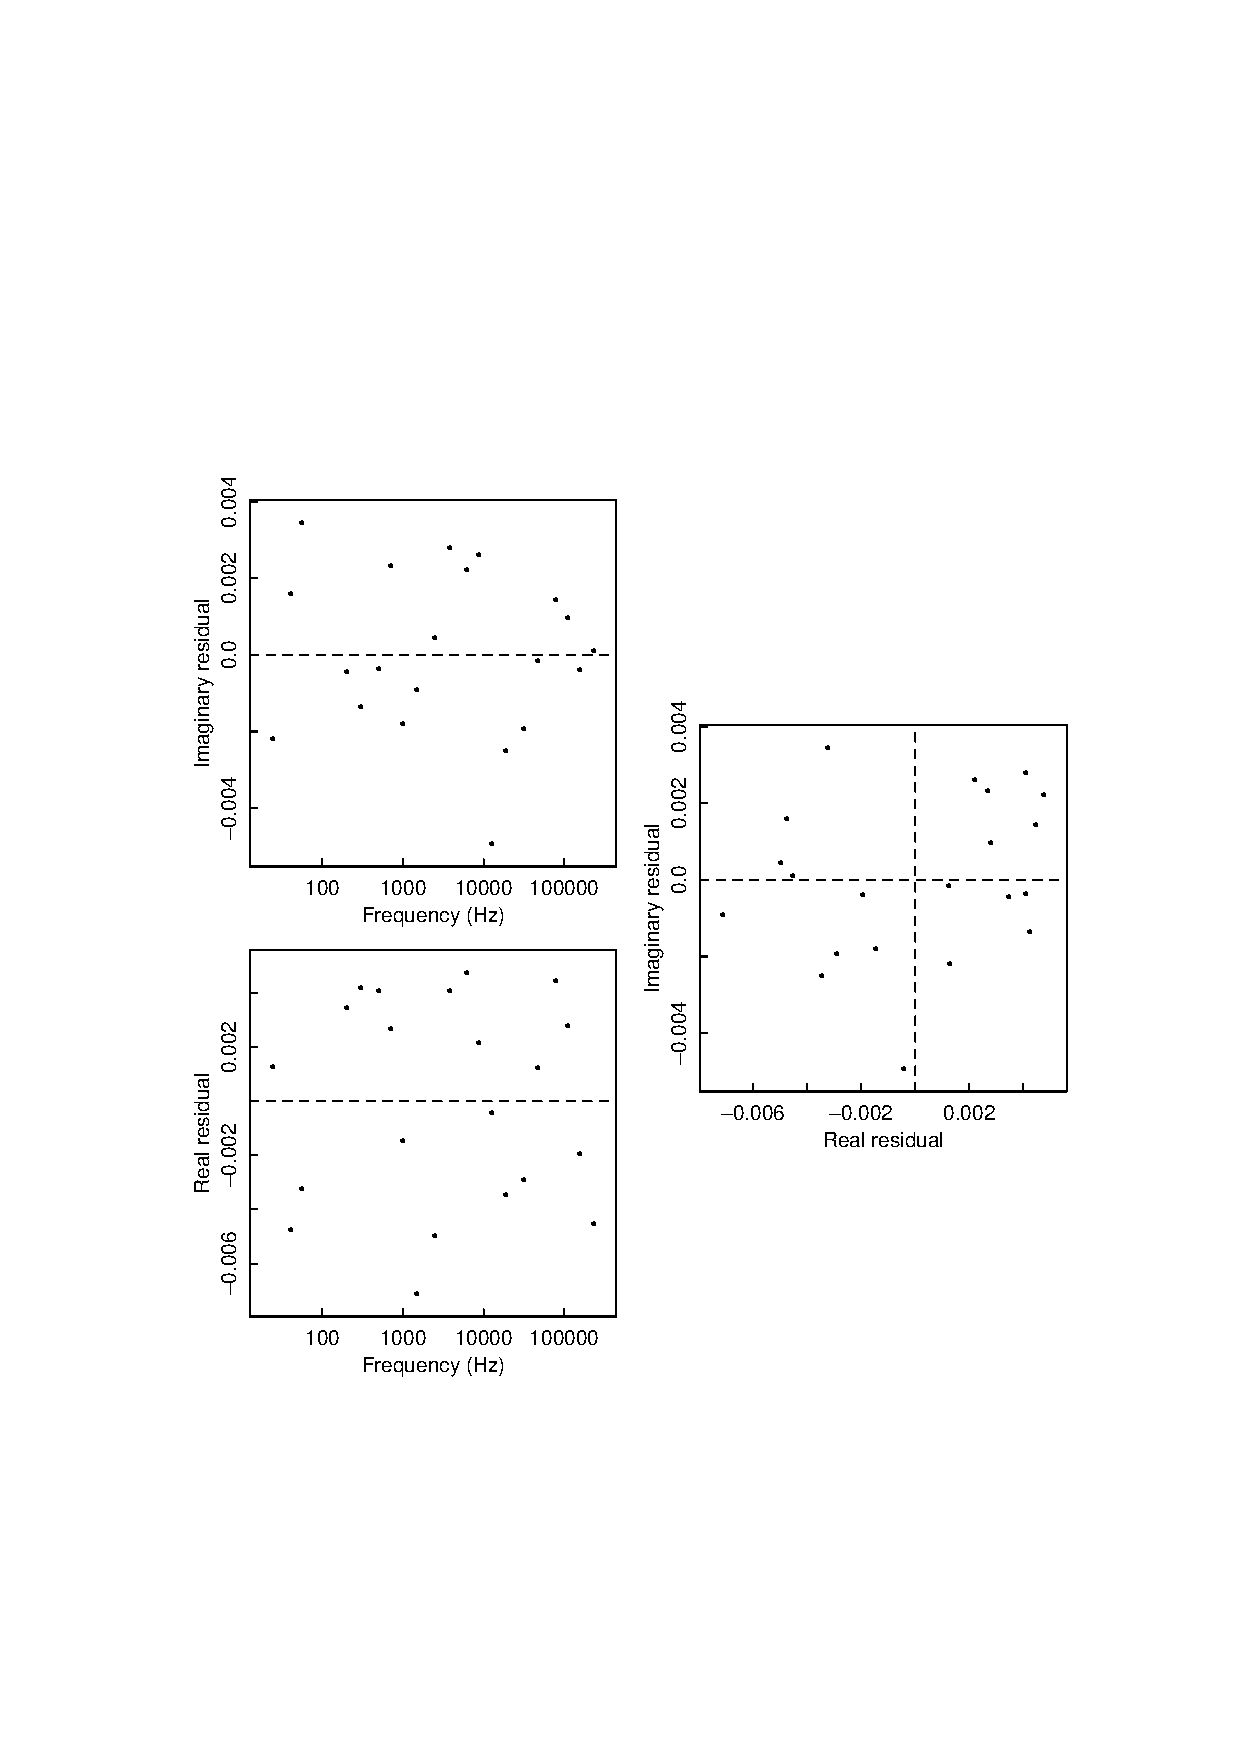
\includegraphics{4PMMAres3}}%,height=4.5in}}
  \caption{\label{fig:PMMAres3}
  Residuals from the fit to the decade-corrected and edited s-PMMA data.}
\end{figure}

We also analyzed the data by estimating $K$ rather than
obtaining it from a search.
The optimum value was $\hat K=1.24$;
the other parameter estimates and their approximate standard errors
changed slightly.
\end{example}

\begin{example}\label{pin:3}

The starting values in Example $\alpha$-Pinene 2 were used together with
the techniques described in
Chapter 5 for obtaining the expectation function and derivatives, and
convergence was obtained for the five response data set as shown
in Table~\ref{tbl:4.5}.
\begin{table}
  \caption{\label{tbl:4.5}
  Parameter summary for the -pinene data using five responses}
  \begin{center}
    \begin{tabular}{ccrrrrrrrr}\hline
      \multicolumn{2}{c}{Parameter} & \multicolumn{1}{c}{$\theta$} &
      \multicolumn{7}{c}{Logarithm Scale}\\
      \multicolumn{1}{c}{From} &\multicolumn{1}{c}{To} &
      \multicolumn{1}{c}{$( 10^{-5} )$}  & \multicolumn{1}{c}{$\phi$}
      & \multicolumn{1}{c}{Std.Error} & \multicolumn{5}{c}{Correlation}\\ \hline
      1&2&3.74&--10.19&0.085&1.00\\
      1&3&1.95&--10.85&0.073&0.84&1.00\\
      3&4&1.65&--11.01&0.104&--\/0.20&--\/0.41&1.00\\
      3&5&27.01&--8.217&0.128&0.00&--\/0.00&0.85&1.00\\
      5&3&2.61&--10.55&0.195&0.68&0.78&--\/0.01&0.40&1.00\\ \hline
    \end{tabular}
  \end{center}
\end{table}
In Figure~\ref{fig:BHME5pred}
\begin{figure}
  \centerline{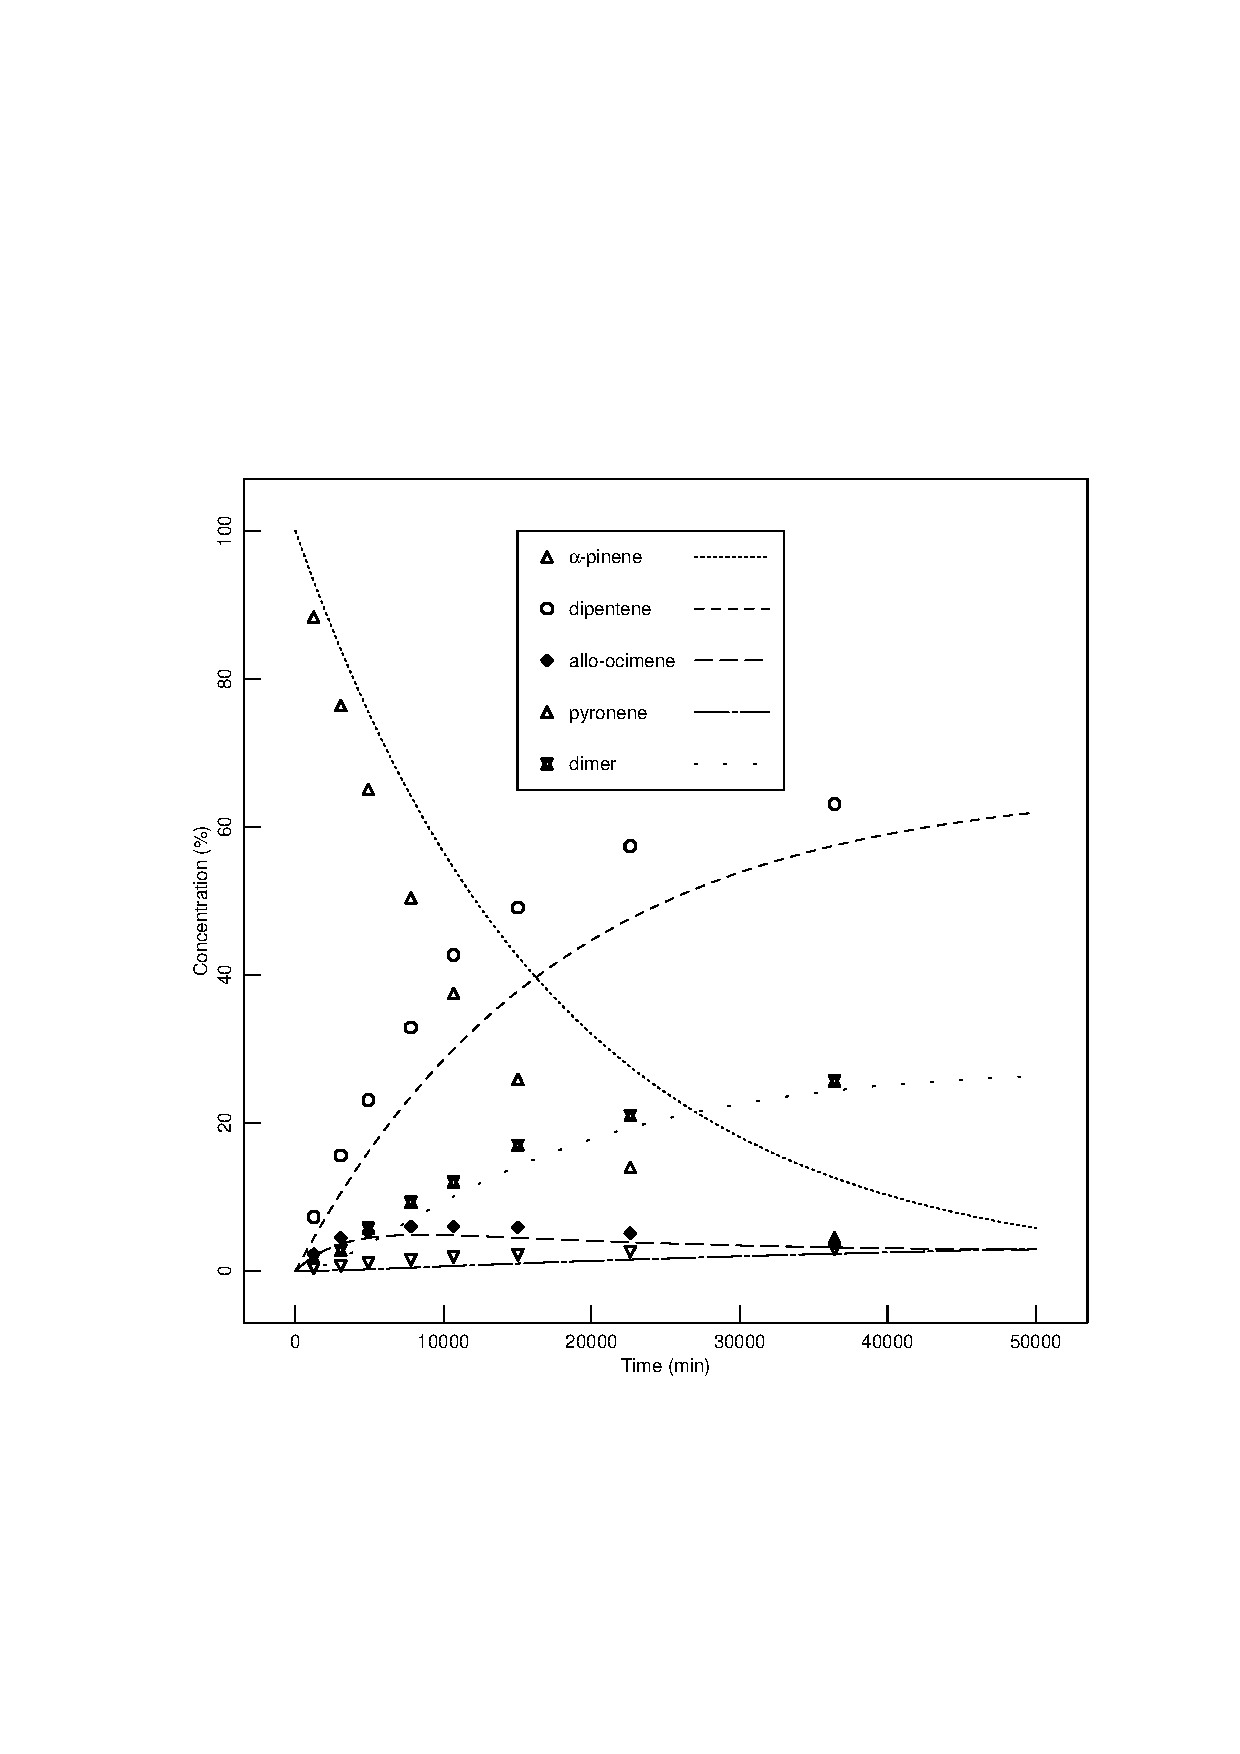
\includegraphics{4BHME5pred}}%,height=4.5in}}
  \caption{\label{fig:BHME5pred}
  Observed values and the predicted curves obtained by fitting five
  responses to the $\alpha$-pinene data}
\end{figure}
we show a plot of the data and the fitted
responses.
The fitted curves do not follow the data very well, suggesting
that convergence to a spurious optimum has occurred.
As will be shown in the next section, this has occurred
because there are dependencies in the data.
\end{example}

\subsection{Dependencies Among Responses}
\index{dependencies!in multiresponse data}
\index{multiresponse estimation!dependencies in data}

Convergence to a spurious optimum due to dependencies in the response data
\index{convergence!to spurious optimum}
is an important problem which can easily arise in multiresponse
estimation, but which can not happen in uniresponse estimation.
Data dependencies can occur, for example, because the responses are
\index{dependencies!in multiresponse estimation}
constrained through mass balances or because one or more responses
are not measured but are imputed from other measured responses.
If dependencies occur in the data or in the expected responses,
then the estimation procedure must be modified so as to avoid
convergence to spurious optima
\cite{box:hunt:macg:erja:1973,mcle:prit:baco:down:1979}.
%\glossary{ Box, G.E.P.}
%\glossary{ Hunter, W.G.}
%\glossary{ MacGregor, J.M.}
%\glossary{ Erjavec, J.}
%\glossary{ McLean, D.D.}
%\glossary{ Pritchard, D.J.}
%\glossary{ Bacon, D.W.}
%\glossary{ Downie, J.}

To detect dependencies in a multiresponse data set,
\citeasnoun{box:hunt:macg:erja:1973}
%\glossary{ Box, G.E.P.}
%\glossary{ Hunter, W.G.}
%\glossary{ MacGregor, J.M.}
%\glossary{ Erjavec, J.}
used an eigenvalue analysis of the
\index{eigenvalue!analysis of centered data matrix}
inner product of the centered data matrix,
\index{matrix!centered data}
$( \bar \bY ) \trans ( \bar \bY )$,
where $\bar \bY$ is the matrix of response averages
obtained by replacing each column of $\bY$ by the average of the column.
They then compared the eigenvalues with an estimate of the roundoff
sum of squares,
$( N-1 ) u^2 / 12 $,
where $u$ is the rounding unit of the data.
Any eigenvalues which were of the same magnitude as the roundoff sum
of squares were
assumed to be associated with linear dependencies in the data.

This approach can reveal singularities
\index{singular!data matrix}
due to conditions that cause a linear combination of the
responses from all cases to be a constant (for example, a mass balance),
but, as described in \citeasnoun{mcle:prit:baco:down:1979}
%\glossary{ McLean, D.D.}
%\glossary{ Pritchard, D.J.}
%\glossary{ Bacon, D.W.}
%\glossary{ Downie, J.}
analysis of the centered {\em data\/} matrix
can fail to detect singularities in the {\em residual\/}
matrix, and hence
\index{singular!residual matrix}
\index{residual!matrix}
\index{matrix!residual}
\index{matrix!singular}
one may still be trying to converge with a ``defective''
data set.
As was also pointed out by these authors, in certain circumstances
linear dependencies among the data need not cause singularities in
the residual matrix $\bZ ( \btheta ) $,
so removal of singularities detected through analysis of the centered data
matrix can cause unnecessary loss of precision in the parameter estimates.
Therefore, it is necessary to search for singularities in
both the centered data matrix and the residual matrix.

As an example where there can be singularities in
$\bZ$ but no singularities in $ \bar \bY $, following
\citeasnoun{mcle:prit:baco:down:1979}, we consider a chemical reaction
%\glossary{ McLean, D.D.}
%\glossary{ Pritchard, D.J.}
%\glossary{ Bacon, D.W.}
%\glossary{ Downie, J.}
in which two responses are measured.
The two responses are normalized
so that the total for the $n$th case is $\gamma_n^{0}$,
the initial concentration of the first chemical.
Unless the initial concentrations are all the same, the matrix
$ \bY - \bar \bY $ will not be singular.
However, if the reaction follows first order kinetics so that
$f_{n1}=\gamma_n^0 e^{{-} \theta t_n }$ and
$f_{n2}=\gamma_n^0 ( 1 - e^{ - \theta t_n } )$,
then the residual matrix $\bZ$ with $n$th row
$$
( z_{n1} , z_{n2} ) =
( y_{n1} - f_{n1} ,  y_{n2} - f_{n2} )
$$
involves the linear dependency $z_{n1}+z_{n2}=0$
for all $n$, and the residual matrix is singular.
It would be futile, therefore, to try to estimate the parameter $\btheta$
using a multiresponse estimation criterion.

As an example where there can be singularities in
$ \bY - \bar \bY $ but no singularities in $\bZ$,
suppose that in the example above, the
two responses are obtained from chromatograph area
fractions, so the measurement for $y_{n1} $ is
$$
y_{n1} = a_1 +
b_1 \left({{\rm area}_{n1} \over {\rm area}_{n1+{\rm }} area_{n2}}
\right)
$$
and that for $ y_{n2} $ is
$$
y_{n2} = a_2 +
b_2 \left({{\rm area}_{n2} \over {\rm area}_{n1+{\rm }} area_{n2}}
\right)
$$
where $a_{1}$, $b_{1}$, $a_{2}$, and $b_{2}$ are calibration
constants.
Then a linear dependency will exist in the data of the form
$ b_2  y_{n1}+b_1 y_{n2} = \mbox{\rm constant}$ for all n, and so $  \bY - \bar \bY  $ will be singular.
However, unless for every case
$$
 \gamma_n^0 \left[ b_1 + ( b_2 - b_1 )
e^{ - \theta t_n } \right] =
a_2 b_1 + a_1 b_2 + b_1 b_2
$$
the residual matrix will not be singular because of the linear
dependence in the data.

Singularities in $ \bY - \bar \bY $ and in $\bZ$ can be detected by
performing an eigenvalue--eigenvector decomposition of the inner
product, as proposed by
\citeasnoun{box:hunt:macg:erja:1973},
%\glossary{ Box, G.E.P.}
%\glossary{ Hunter, W.G.}
%\glossary{ MacGregor, J.M.}
%\glossary{ Erjavec, J.}
but we prefer to arrange the rounding units in the columns of $\bY$ to
be approximately equal and then take singular value decompositions of
\index{singular value decomposition}
$ \bar \bY $ and $\bZ$ \cite[Chapter 11]{dong:bunc:mole:stew:1979}.
%\glossary{ Dongerra, J.J.}
%\glossary{ Bunch, J.R.}
%\glossary{ Moler, C.B.}
%\glossary{Stewart, G.W.}
As explained there, singular values on the order of
the rounding unit indicate singularity and should prompt the
analyst to search for dependencies in the data.

A singular value decomposition of the centered data matrix, and
of the residual matrix using the initial parameter values,
should be done at the beginning of the analysis so as to avoid
unnecessary calculations caused by dealing with a defective
data set which involves linear dependencies.
If small singular values are obtained, the corresponding singular
vectors should be examined to reveal what is causing the
dependencies.
If the dependency can be explained (e.g., a mass balance, or a response
has been imputed from other measured responses) and the offending
responses identified, they should be removed and a multiresponse
analysis performed on the reduced data set.
If a dependency can not be explained, then the multiresponse analysis
should be modified to take account of the dependency as described
in Section 4.3.4.
The residual matrix at the converged parameter values
should also be analyzed for singular values
so as to detect possible dependencies in the residuals.
Further comments on detecting and eliminating linear
dependencies are given in
\citeasnoun{mcle:prit:baco:down:1979}.
%\glossary{ McLean, D.D.}
%\glossary{ Pritchard, D.J.}
%\glossary{ Bacon, D.W.}
%\glossary{ Downie, J.}

\begin{example}\label{spmma:4}
For the decade-corrected and edited s-PMMA data, the singular
values of the centered data matrix
are 0.278 and 2.161, and since
the rounding units in the data are both 0.001,
neither of these singular values is small
enough to suggest a linear dependency.
The singular values of the residual matrix at the converged values
are 0.009 and 0.017 and neither of these is small enough to cause
concern.
\end{example}

\begin{example}\label{pin:4}
The centered data matrix for the $\alpha$-pinene data, has the
singular value decomposition
%Singular value:0.04:0.13:1.10:5.08:98.30
%_
%Singular vectors:\-\^0.17:0.48:\-\^0.30:0.06:\-\^0.81
%\^:\-\^0.21:0.49:\-\^0.61:\-\^0.22:0.54
%\^:\-\^0.16:0.43:0.64:\-\^0.61:0.01
%\^:0.93:0.36:\-\^0.01:0.00:0.02
%\^:\-\^0.19:0.46:0.36:0.76:0.23
%.TE
which clearly indicates dependencies in the data because
the two small singular values are of the same magnitude as
the rounding unit in the data (0.1, see Appendix 1, Section A1.6).

The residual matrix at the starting estimates has
the singular value decomposition
%Singular value:0.06:0.14:0.46:1.63:42.70
%_
%Singular vectors:0.34:\-\^0.30:\-\^0.28:0.26:0.81
%\^:0.39:\-\^0.26:\-\^0.39:0.55:\-\^0.57
%\^:0.60:\-\^0.27:0.75:\-\^0.08:\-\^0.07
%\^:\-\^0.50:\-\^0.86:0.08:\-\^0.05:\-\^0.06
%\^:0.36:\-\^0.20:\-\^0.45:\-\^0.79:\-\^0.12
which also reveals two dependencies.

As noted by \citeasnoun{box:hunt:macg:erja:1973}, from careful reading of the
%\glossary{ Box, G.E.P.}
%\glossary{ Hunter, W.G.}
%\glossary{ MacGregor, J.M.}
%\glossary{ Erjavec, J.}
paper by \citeasnoun{fugu:hawk:1947}, the response $y_4 $ was
%\glossary{ Fuguitt, R.E.}
%\glossary{ Hawkins, J.E.}
not in fact measured, but was imputed as 3\% of the
amount of converted $y_{1}$, i.e.,
$y_4=$ $0.03 ( 100 - y_1 )$.
The first singular vector of the centered data matrix reflects this
dependency and so
the imputed data for $y_4 $ should not be used in estimation.
The second singular vector, consisting of almost equal entries,
reflects a mass balance dependency, i.e., the data must sum to
100\%.
This occurs because the system is a conservative one, as can
easily be seen, since all the columns of the system matrix $\bA$
sum to zero.
The singular vectors of the residual matrix do not reflect these
dependencies, so that while the singular value decomposition of $\bZ$
does suggest that there are dependencies, it does not reveal their
nature.

Because there are two small singular values, suggesting two
linear dependencies in the data, only three responses
should be retained for parameter estimation.
\end{example}

When linear dependencies are found, the problem of
choosing an appropriate subset of the responses must be addressed.
One approach is to retain those responses which the researcher
thinks are most reliable.
It may not be possible to select the responses on this basis, however,
and so we follow \citeasnoun{box:hunt:macg:erja:1973} and use
%\glossary{ Box, G.E.P.}
%\glossary{ Hunter, W.G.}
%\glossary{ MacGregor, J.M.}
%\glossary{ Erjavec, J.}
a linear combination of the responses instead.
In either situation, it would be helpful to have a procedure for
estimating parameters in the presence of dependencies.
Accordingly, in the following section we describe a procedure for
estimating parameters in the presence of linear dependencies.

\subsection{Linear Combinations of Responses}
\index{dependencies!in multiresponse estimation}

Suppose there are $d$ linear dependencies, and there are no missing
values in the data matrix.
To deal with linear dependencies,
we generate an $N \times ( M - d )$ reduced residual matrix
$\bZ \bB$ by combining the $d$ linear dependency
vectors into an $M \times d$ dependency matrix $\bD$, performing a $QR$
decomposition
on $\bD$, and letting the rotation matrix $\bB$ be the $ M-d $
columns of $\bQ$ which are orthogonal to the dependency vectors.

\begin{example}\label{pin:5}
For the $\alpha$-pinene data, we have decided that response 4
should not be used in estimation, and that there is a mass
balance relation in the data.
The dependency matrix is therefore
$$
\bD = \left[ \matrix {
\matrix { 0 \cr 0 \cr 0 \cr 1 \cr 0 }
\matrix { 1 \cr 1 \cr 1 \cr 1 \cr 1 }
}\right]
$$
Performing a $QR$ decomposition produces $\bB$ as the last three
columns of $\bQ$.
Again, as discussed in Appendix 2, although $\bQ$ is required to obtain
$\bB$, $\bQ$ is not explicitly formed; a product
such as $\bZ_{(p)} \bB$ is formed by applying Householder
transformations to $\bZ_{(p)} \trans $, retaining the last $M - d$
rows to give $( \bZ_{(p)} \bB ) \trans$, and then transposing the result.
\end{example}

To minimize $ | ( \bZ \bB ) \trans ( \bZ \bB ) |$ using the generalized
Gauss--Newton method of Section 4.2, we need $( \bZ \bB )_{(p)} $.
This is easily obtained because $\bB$ is independent of $\btheta$, and so
$$
( \bZ \bB )_{(p)} = \bZ_{(p)} \bB
$$
Thus, the terms in the determinant, the gradient and the approximate
Hessian for the reduced data set can be calculated by simply using
$ \bZ $ and $ \bZ_{(p)} , p = 1 ,\ldots, P$.

\begin{example}\label{pin:5a}
Using the starting values from Example $\alpha$-Pinene \ref{pin:3} and
three (rotated) responses, we obtained the results in
Table~\ref{tbl:4.6}.
\begin{table}
  \caption{\label{tbl:4.6}
  Parameter summary for the $\alpha$-pinene data using three rotated
  responses}
%c s c c s s s s s s
%c s c c s s s s s s
%c1 c c c1 c c s s s s
%c1 c n n1 n n1 n1 n1 n1 n.
%\_
%Parameter:$\theta$:Logarithm Scale
%From:To:$( 10^{-5} )$:$\phi$:Std.Error:Correlation
%\_
%1:2:5.94:--9.731:0.021:1.00
%1:3:2.86:--10.47:0.042:--\/0.20:1.00
%3:4:0.453:--12.31:3.92:--\/0.37:0.91:1.00
%3:5:31.12:--8.072:0.124:--\/0.22:0.51:0.45:1.00
%5:3:5.79:--9.757:0.21:0.10:0.16:0.16:0.78:1.00
%\_
\end{table}
The overlay plot of the data and fitted curves in
Figure~\ref{fig:BHME3pred}
  \begin{figure}
    \centerline{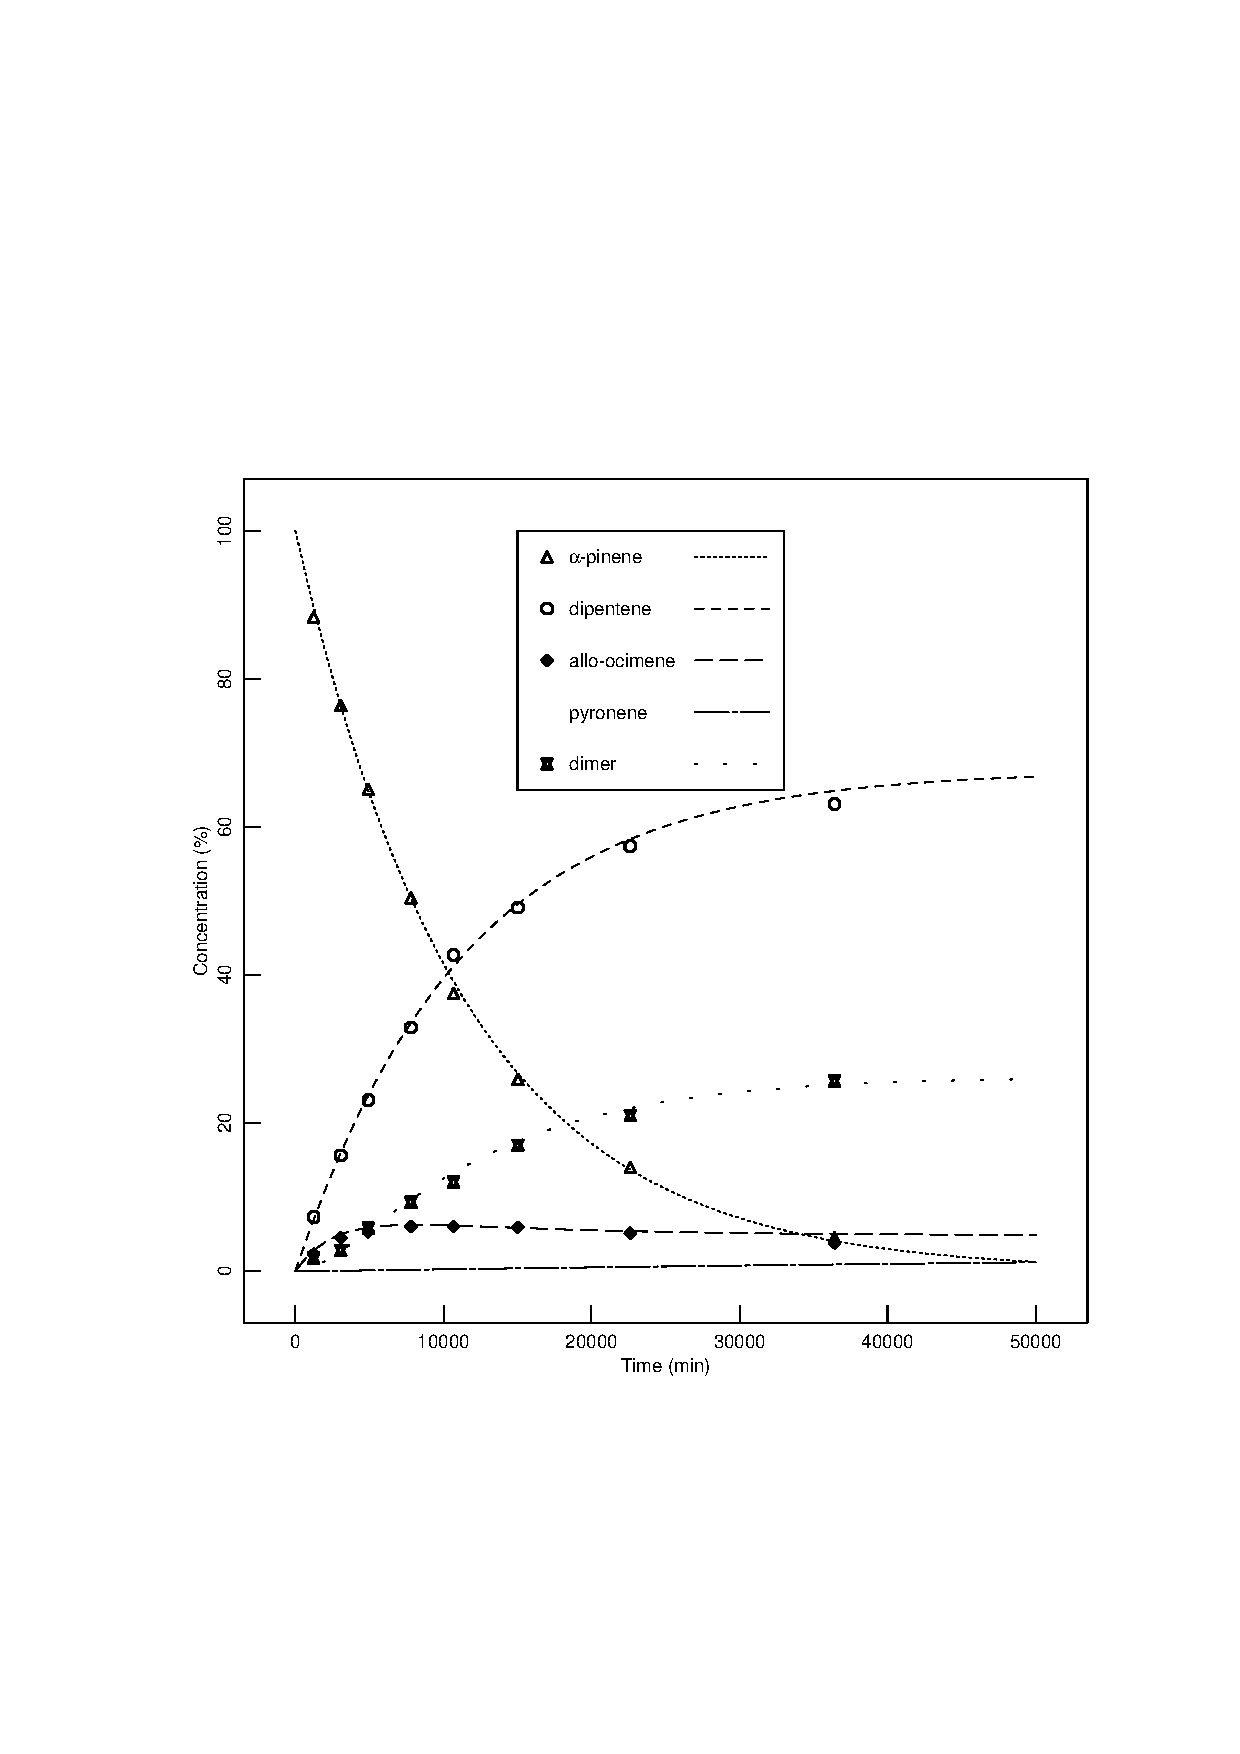
\includegraphics{4BHME3pred}}%,height=4.5in}}
    \caption{\label{fig:BHME3pred}
    Observed values and the predicted curves obtained by fitting three
    rotated responses to the $\alpha$-pinene data.
    }
  \end{figure}
gives no evidence of inadequacy of the fitted model.
However, the residuals, shown in Figure~\ref{fig:BHME3res},
  \begin{figure}
    \centerline{\includegraphics{4BHME3res}}%,width=\textwidth}}
    \caption{\label{fig:BHME3res}
    Residuals from the three rotated response fit to the $\alpha$-pinene
    data plotted versus time and versus predicted response.
    }
  \end{figure}
are not well behaved, with a large negative residual for response 3 and
a trend and a large positive residual for response 2.
There is also a preponderance of negative residuals.
Also the approximate confidence limits on $\phi_{3}$ are
very wide, suggesting that it is badly estimated and that $\theta_{3}$
could be zero.
We temporarily ignore the defective residuals, and try to see if a
simpler model would be adequate.
\end{example}

Linear combinations of responses can be used to check for consistency of
information by analyzing subsets of the responses, as suggested in
\citeasnoun{box:drap:1965}.
%\glossary{ Box, G.E.P.}
%\glossary{ Draper, N.R.}
We simply let $\bB$ be the matrix derived from an identity
matrix by deleting columns corresponding to the unused responses.

\begin{example}\label{pin:5b}
Suppose we wished to estimate the
parameters using only the responses $y_{1}$, $y_{2}$, and $y_{5}$.
Then we would use as the rotation matrix
$$
\bB = \left[ \matrix {
\matrix { 1 \cr 0 \cr 0 \cr 0 \cr 0 }
\matrix { 0 \cr 1 \cr 0 \cr 0 \cr 0 }
\matrix { 0 \cr 0 \cr 0 \cr 0 \cr 1 }
}\right]
$$
\end{example}

\subsection{Comparing Models}

Nested models can be compared using an
\index{model!nested}
``extra determinant''
\index{extra determinant!test for nested models}
\index{nested model!extra determinant test}
analysis in the same way that uniresponse nested models were compared
using an extra sum of squares analysis (Section 3.10).
That is, we compare the ratio of the change in the determinant divided
by the change in the degrees of freedom with the scaled determinant
for the complete model as in (\ref{eqn:Fregion}).

\begin{example}\label{pin:6}
The model for the $\alpha$-pinene reaction includes a path from species
3 to species 4, but as seen in Example $\alpha$-Pinene~\ref{pin:5},
the logarithm of the rate constant associated with that path has a
large standard error, suggesting that this path could be eliminated.
Fitting the data without this path, but still retaining only three
(rotated) responses, gives the results in
Table~\ref{tbl:4.7}.
\begin{table}
  \begin{center}
    \begin{tabular}{ccrrrrrrr}\hline
      \multicolumn{2}{c}{Parameter} & \multicolumn{1}{c}{$\theta$} &
      \multicolumn{6}{c}{Logarithm Scale}\\
      \multicolumn{1}{c}{From} &\multicolumn{1}{c}{To} &
      \multicolumn{1}{c}{$( 10^{-5} )$}  & \multicolumn{1}{c}{$\phi$}
      & \multicolumn{1}{c}{Std.Error} & \multicolumn{4}{c}{Correlation}\\ \hline
      1&2&5.94&--9.73&0.018&1.00\\
      1&3&2.82&--11.28&0.016&0.44&1.00\\
      3&5&30.75&--8.09&0.093&--\/0.07&0.26&1.00\\
      5&3&5.72&--9.77&0.182&0.16&0.05&0.81&1.00\\ \hline
    \end{tabular}
  \end{center}
\end{table}
Combining these results with the results in Table~\ref{tbl:4.6}
allows us to perform an extra determinant analysis as in
Table~\ref{tbl:4.8a}.
\begin{table}
  \caption{\label{tbl:4.8a}
  Extra determinant analysis of the 4-parameter model versus
  the 5-parameter model for the $\alpha$-pinene data.}
  \begin{center}
    \begin{tabular}{lccccc}\hline
      && \multicolumn{1}{c}{Degrees of} & \multicolumn{1}{c}{Mean}\\
      \multicolumn{1}{c}{Source} & \multicolumn{1}{c}{Determinant} &
      \multicolumn{1}{c}{Freedom} & \multicolumn{1}{c}{Det.} &
      \multicolumn{1}{c}{F Ratio} & \multicolumn{1}{c}{$p$ Value}\\ \hline
      Extra&0.60&1&0.60&0.06&0.822\\
      Full model&28.39&3&9.46\\ \hline
      partial model&28.99&4\\ \hline
    \end{tabular}
  \end{center}
\end{table}
According to this analysis, the extra path is not necessary.

The predicted response curves are plotted in
Figure~\ref{fig:BHME4path}.
\begin{figure}
  \centerline{\includegraphics{4BHME4path}}%,height=4.5in}}
  \caption{\label{fig:BHME4path}
  Observed values and the predicted curves obtained by fitting three
  rotated responses to the $\alpha$-pinene data, eliminating pyronene
  production.}
\end{figure}
The residuals for this model are almost identical to those from the
previous fit, and so we could reanalyze the data, treating the
observations with the large residuals as missing.
\end{example}

\begin{problems}
  
  \prob
  Write a computer routine in a language of your choice to
  calculate the determinant, the gradient of the determinant, and the
  approximate Hessian of the determinant, for a multiresponse
  estimation routine.  If necessary, use the pseudocode in Appendix 3,
  Section A3.3 for guidance.
  
  \prob Use the data for responses 1 and 2 in the $\alpha$-pinene data
  set, Appendix 4, Section A4.6, to fit the multiresponse model
  $$
  \bgamma( t )=\left[ \matrix{
      \matrix {e^{{-} ( \theta_1 +\theta_2 )t} \cr
        {\theta_1 \over \theta_1 +\theta_2}
        \left( 1-e^{{-} ( \theta_1 +\theta_2 )t}\right)}
    }\right]
  $$
  Assume the initial concentration of $\alpha$-pinene (response 1)
  is 100\% and of dipentene (response 2) is 0\%.
  
  \subprob Use the approximate rate procedure of Section 4.3.1 to
  obtain starting estimates for the parameters.
  
  \subprob Use a nonlinear estimation routine to obtain the parameter
  estimates.  Replace the missing value for response 1 at time $16020$
  by 0 to obtain the parameter estimates.
  
  \subprob Use the procedure in Section 4.4 to estimate the parameters
  and the missing value.
  
  \prob Perform a singular value decomposition of the centered data
  matrix for the data from Appendix 4, Section A4.7, to determine if
  there are any linear dependencies in the data.
  
  \prob For the data and model of Problem 4.2, the parameter estimates
  and summary statistics from part (b) are as follows:

  \begin{center}
    \begin{tabular}{ccrccc} \hline
      && \multicolumn{3}{c}{Logarithm Scale}\\
      &&& \multicolumn{1}{c}{Std.} & \multicolumn{1}{c}{Correlation}\\
      \multicolumn{1}{c}{Parameter} & \multicolumn{1}{c}{Estimate} &
      \multicolumn{1}{c}{$ln\theta$}& \multicolumn{1}{c}{Error} &
      \multicolumn{1}{c}{Matrix}\\ \hline
      $\theta_{1}$&0.000221&--8.417&0.0085&1.00\\
      $\theta_{2}$&0.000139&--8.881&0.0059&0.69&1.00\\ \hline
    \end{tabular}
  \end{center}

  \subprob Calculate joint and marginal 95\% inference regions for the
  parameters using equations (4.9) and (4.12).
  
  \subprob Use a grid of values of $ln\theta_1 $ from $-8.46$ to
  $-8.38$ in steps 0.005 and $ln\theta_2 $ from $-8.904$ to $-8.854$
  in steps of 0.002, and calculate the determinant at each point.
  Join points of equal value to delineate contours.
  
  \subprob Plot the joint 95\% inference region from part (a) on the
  contour plot in part (b).  Is the linear approximation region
  accurate in this case?
  
  \prob Use the data and model from Appendix 4, Section A4.7 to fit a
  multiresponse model.  Reduce the model to a simple form by
  eliminating parameters which could be zero.  Your analysis to
  Problem 4.3 should have alerted you to the fact that there was a
  dependency in the data.  In fact, the water component $y_{6}$ was
  imputed from a mass balance equation, and so this response should
  not be used in fitting the model.  Because of this, it is convenient
  to estimate the parameters $\theta_{6}$ and $\beta_{6}$ from the
  parameter constraint equations.
\end{problems}


% Local Variables: 
% mode: latex
% TeX-master: "nraia2"
% End: 

\chapter[Differential Equations]{Models Defined by Systems
of Differential Equations}

\prologue{The universe is like a safe to which there is a combination,
but the combination is locked up in the safe.}{Peter de Vries}

An important class of models is that in which the responses are
described by a linear system of ordinary differential
\index{model!linear differential equations}
equations.
These models are used in chemical kinetics
\cite{from:bisc:1979} and in pharmacokinetics
%\glossary{ Froment, G.F.}
%\glossary{ Bischoff, K.B.}
\cite{godf:1983},
%\glossary{ Godfrey, K.}
where they are called {\em compartment\/} models.
\index{compartment model}
Because they are used in so many areas, it is worthwhile to have
special techniques to make their analysis easier.
Accordingly, in this chapter we present efficient methods for
estimating parameters in compartment models and for developing
and testing competing models.
Techniques for dealing with systems of nonlinear differential
equations are discussed in \citeasnoun{bard:1974} and
\citeasnoun{cara:stew:1985}.
%\glossary{ Bard, Y.}
%\glossary{ Caracotsios, M.}
%\glossary{ Stewart, W.E.}

\section{Compartment Models and System Diagrams}

A common use of compartment models is in pharmacokinetics,
where the exchange of materials
in biological systems is studied.
A system is divided into compartments, and
it is assumed that the rates of flow of drugs between
compartments follow first order kinetics, so that the rate of
transfer to a receiving, or {\em sink}, compartment is proportional
to the concentration in the supplying, or {\em source}, compartment.
\index{compartment model!sink}
\index{compartment model!source}
The transfer coefficients, which are assumed constant with respect to
time, are called {\em rate constants}.
\index{rate constant}

\begin{example}\label{tet:1}
  
As an example of a compartment model, we consider data on the
concentration of tetracycline hydrochloride in serum.  A
tetracycline compound was administered to a subject orally, and the
concentration of tetracycline hydrochloride in the serum was
measured over a period of 16 hours \cite{wagn:1967}.
The data are recorded in Appendix A, Section~\ref{atbl:tet},
and plotted in Figure \ref{fig:TETdata}.
\begin{figure}[tbp]
  \centerline{\includegraphics{5TETdata}}%,height=4in}}
  \caption{\label{fig:TETdata}
  Plot of tetracycline concentration versus time.}
\end{figure}


The biological system can be modeled by a gut compartment into
which the chemical is introduced, a blood compartment which
absorbs the chemical from the gut, and an elimination path.
Assuming first order kinetics, the concentrations
$( \gamma_1 (t) , \gamma_2 (t) ) \trans$
of tetracycline hydrochloride in the two compartments
can be described by the following pair of differential equations:
\begin{eqnarray} \label{eqn:5.1}
  \frac{d\gamma_1(t)}{d t}&=&
  \dot \gamma_1 = - \theta_1 \gamma_1 ( t )\\
  \frac{d\gamma_2(t)}{d t}&=&
  \dot \gamma_2 =
  \theta_1 \gamma_1 ( t ) - \theta_2 \gamma_2 ( t )\nonumber
\end{eqnarray}
where the dot denotes differentiation with
respect to time.

The system can be represented graphically as a compartment or system
diagram as in Figure \ref{fig:tet}.
\index{system diagram}
\expandafter\ifx\csname graph\endcsname\relax \csname newbox\endcsname\graph\fi
\expandafter\ifx\csname graphtemp\endcsname\relax \csname newdimen\endcsname\graphtemp\fi
\setbox\graph=\vtop{\vskip 0pt\hbox{%
    \special{pn 8}%
    \special{ar 250 250 250 250 0 6.28319}%
    \graphtemp=.5ex\advance\graphtemp by 0.250in
    \rlap{\kern 0.250in\lower\graphtemp\hbox to 0pt{\hss $\gamma_{1}$\hss}}%
    \special{pa 500 250}%
    \special{pa 1000 250}%
    \special{fp}%
    \special{sh 1.000}%
    \special{pa 900 225}%
    \special{pa 1000 250}%
    \special{pa 900 275}%
    \special{pa 900 225}%
    \special{fp}%
    \graphtemp=\baselineskip\multiply\graphtemp by -1\divide\graphtemp by 2
    \advance\graphtemp by .5ex\advance\graphtemp by 0.250in
    \rlap{\kern 0.750in\lower\graphtemp\hbox to 0pt{\hss $\theta_{1}$\hss}}%
    \special{ar 1250 250 250 250 0 6.28319}%
    \graphtemp=.5ex\advance\graphtemp by 0.250in
    \rlap{\kern 1.250in\lower\graphtemp\hbox to 0pt{\hss $\gamma_{2}$\hss}}%
    \special{pa 1250 500}%
    \special{pa 1250 1000}%
    \special{fp}%
    \special{sh 1.000}%
    \special{pa 1275 900}%
    \special{pa 1250 1000}%
    \special{pa 1225 900}%
    \special{pa 1275 900}%
    \special{fp}%
    \graphtemp=.5ex\advance\graphtemp by 0.750in
    \rlap{\kern 1.250in\lower\graphtemp\hbox to 0pt{\hss $\theta_{2}$ }}%
    \hbox{\vrule depth1.000in width0pt height 0pt}%
    \kern 1.500in
  }%
}%

\begin{figure}
  \centerline{\box\graph}
  \caption{\label{fig:tet}
  A compartment or system diagram for the tetracycline model.}
\end{figure}
\end{example}

Chemical reactions can also be described by linear systems of first
order differential equations.
In this context, the chemical species
of the reaction constitute the compartments, the original species
being termed ``parents,''
and the product species ``daughters.''

\begin{example}\label{oil:1}

As a chemical example, we consider the pyrolysis of oil shale
described by \citeasnoun{zieg:gorm:1980}.
%\glossary{ Ziegel, E.R.}
%\glossary{ Gorman, J.W.}
Oil shale contains organic material which is organically bonded to the
structure of the rock.
To extract oil from the rock, heat is applied so the technique is
called pyrolysis.

During pyrolysis, the benzene organic material, called kerogen,
decomposes to oil and bitumen, and there are unmeasured by-products of
insoluble organic residues and light gases.
Ziegel and Gorman, using data obtained from
\citeasnoun{hubb:robi:1950}, estimated the rate constants in several
%\glossary{ Hubbard, A.B.}
%\glossary{ Robinson, W.E.}
candidate models.
The data obtained by Hubbard and Robinson are listed
in Appendix A, Section~\ref{atbl:oil}.

The final model fitted by Ziegel and Gorman to the 400$^\circ$C data
using multiresponse
estimation techniques can be represented by the system diagram
in Figure \ref{fig:ziggy},
which corresponds to the set of linear differential
equations,
\begin{eqnarray}\label{eqn:5.2}
  \frac{d\gamma_1}{dt}&=&-(\theta_1+\theta_4)\gamma_1\\
  \frac{d\gamma_2}{dt}&=&\theta_1\gamma_1-(\theta_2+\theta_3)\gamma_2\nonumber\\
  \frac{d\gamma_3}{dt}&=&\theta_4\gamma_1+\theta_2\gamma_2\nonumber
\end{eqnarray}
In this equation, $\gamma_1$ denotes kerogen, $\gamma_{2}$
bitumen, and $\gamma_{3}$ oil.
\expandafter\ifx\csname graph\endcsname\relax \csname newbox\endcsname\graph\fi
\expandafter\ifx\csname graphtemp\endcsname\relax \csname newdimen\endcsname\graphtemp\fi
\setbox\graph=\vtop{\vskip 0pt\hbox{%
    \special{pn 8}%
    \special{ar 250 650 250 250 0 6.28319}%
    \graphtemp=.5ex\advance\graphtemp by 0.650in
    \rlap{\kern 0.250in\lower\graphtemp\hbox to 0pt{\hss $\gamma_{1}$\hss}}%
    \special{pa 500 650}%
    \special{pa 1000 650}%
    \special{fp}%
    \special{sh 1.000}%
    \special{pa 900 625}%
    \special{pa 1000 650}%
    \special{pa 900 675}%
    \special{pa 900 625}%
    \special{fp}%
    \graphtemp=\baselineskip\multiply\graphtemp by -1\divide\graphtemp by 2
    \advance\graphtemp by .5ex\advance\graphtemp by 0.650in
    \rlap{\kern 0.750in\lower\graphtemp\hbox to 0pt{\hss $\theta_{1}$\hss}}%
    \special{ar 1250 650 250 250 0 6.28319}%
    \graphtemp=.5ex\advance\graphtemp by 0.650in
    \rlap{\kern 1.250in\lower\graphtemp\hbox to 0pt{\hss $\gamma_{2}$\hss}}%
    \special{pa 1500 650}%
    \special{pa 2000 650}%
    \special{fp}%
    \special{sh 1.000}%
    \special{pa 1900 625}%
    \special{pa 2000 650}%
    \special{pa 1900 675}%
    \special{pa 1900 625}%
    \special{fp}%
    \graphtemp=\baselineskip\multiply\graphtemp by -1\divide\graphtemp by 2
    \advance\graphtemp by .5ex\advance\graphtemp by 0.650in
    \rlap{\kern 1.750in\lower\graphtemp\hbox to 0pt{\hss $\theta_{2}$\hss}}%
    \special{ar 2250 650 250 250 0 6.28319}%
    \graphtemp=.5ex\advance\graphtemp by 0.650in
    \rlap{\kern 2.250in\lower\graphtemp\hbox to 0pt{\hss $\gamma_{3}$\hss}}%
    \special{pa 1250 900}%
    \special{pa 1250 1400}%
    \special{fp}%
    \special{sh 1.000}%
    \special{pa 1275 1300}%
    \special{pa 1250 1400}%
    \special{pa 1225 1300}%
    \special{pa 1275 1300}%
    \special{fp}%
    \graphtemp=.5ex\advance\graphtemp by 1.150in
    \rlap{\kern 1.250in\lower\graphtemp\hbox to 0pt{\hss $\theta_{3}$ }}%
    \special{ar 1250 2132 2000 2000 -2.094395 -1.047198}%
    \special{sh 1.000}%
    \special{pa 2176 328}%
    \special{pa 2250 400}%
    \special{pa 2151 372}%
    \special{pa 2176 328}%
    \special{fp}%
    \graphtemp=.5ex\advance\graphtemp by 0.000in
    \rlap{\kern 1.250in\lower\graphtemp\hbox to 0pt{\hss $\theta_{4}$\hss}}%
    \hbox{\vrule depth1.400in width0pt height 0pt}%
    \kern 2.500in
  }%
}%

\begin{figure}
  \centerline{\box\graph}
  \caption{\label{fig:ziggy}
  System diagram for the oil shale pyrolysis model.}
\end{figure}

The model implies that kerogen decomposes to bitumen with rate
constant $\theta_{1}$ and to oil with rate constant
$\theta_{4}$, and that bitumen decomposes to oil with rate constant
$\theta_{2}$ and to unmeasured by-products with rate constant
$\theta_{3}$.
\end{example}

In the general compartment model consisting of $K$ compartments,
we write the concentrations at time $t$ as
$\bgamma(t)=(\gamma_1(t),\ldots,\gamma_K(t))\trans$.
Assuming first order kinetics with rate constants
$\theta_1,\theta_2,\ldots,\theta_P$,
the concentrations obey the linear system of differential
equations
\begin{equation}
  \label{eqn:5.3}
  \frac{d\bgamma}{dt}=\dot{\bgamma}(t)=\bA\bgamma(t)+\biota(t)
\end{equation}
where $\bA$ is the $K \times K$ system {\em transfer matrix\/}
\index{matrix!system transfer}
\index{transfer matrix}
containing the rate constants and $\biota(t)$ is a vector
function representing input to the system.

Although more complicated inputs may be used \cite{bate:wolf:watt:1986},
%\glossary{ Bates, D.M.}
%\glossary{ Wolf, D.A.}
%\glossary{ Watts, D.G.}
in this book we consider only two input functions.
One is a continuous infusion of material or {\em step input\/}
into the system,
\begin{displaymath}
\biota ( t ) = \left\{
\begin{array}{c c}
  \biota&t\ge 0\\
  0&t<0
\end{array}
\right.
\end{displaymath}
where $\biota$ is a constant vector.
The other is a bolus or instantaneous injection, and although it
can be considered as an impulse or Dirac $\delta$-function input, it
is simpler to consider it as determining a vector of initial conditions
$\bgamma(0)=\bgamma_{0}$.

\begin{example}\label{tet:2}

For the tetracycline example, the input is a bolus in the gut,
and the transfer matrix $\bA$ can be readily obtained by
inspection of the differential equations (\ref{eqn:5.1}) or from the system
diagram (Figure \ref{fig:tet}), as
\begin{displaymath}
\bA = \left[
\begin{array}{r r}
  -\theta_1&0\\
  \theta_1&-\theta_2
\end{array}
\right]
\end{displaymath}
The initial concentration of tetracycline hydrochloride in
the gut is unknown, but the concentration in the serum is assumed to be
zero, so we incorporate another parameter $\theta_{3}$ and
write $\bgamma_0=(\theta_3,0)\trans$.
\end{example}

\begin{example}\label{oil:2}

For the model (\ref{eqn:5.2}) suggested by \citeasnoun{zieg:gorm:1980},
%\glossary{ Ziegel, E.R.}
%\glossary{ Gorman, J.W.}
% \begin{displaymath}
% \bA = \left[ \matrix {
% \matrix { { - \theta_1 - \theta_4 } \cr \theta_1 \cr \theta_4 }
% \matrix { 0 \cr { - \theta_2 - \theta_3 } \cr \theta_2 }
% \matrix { 0 \cr 0 \cr 0 }
% }\right]
% \end{displaymath}
The recorded measurements for bitumen and oil are percentages of
the initial amount of kerogen, so we take
$\bgamma_0=(100,0,0)\trans$.
\citeasnoun{zieg:gorm:1980} found it necessary to incorporate
%\glossary{ Ziegel, E.R.}
%\glossary{ Gorman, J.W.}
a fifth parameter in the model to account for the unknown dead
time before the reaction began.
\end{example}

\section{Estimating Parameters in Compartment Models}

Several methods can be used to estimate parameters in compartment
models.
The most obvious is to obtain the analytic solution to
the system of differential equations and then use
the expectation function corresponding to the compartment
for which data are available
in a standard nonlinear estimation program.
A second approach is to use a standard nonlinear estimation
program, but calculate the function by solving the equations using
numerical integration.
A third approach \cite{ande:1983} is to recognize that the
%\glossary{ Anderson, D.H.}
responses $\gamma_1 ,  \gamma_2 ,\ldots, \gamma_{K}$
generally consist of
weighted sums of exponential functions of time, with the
exponents related to the system rate constants $\btheta$.
One can then fit a general sum of exponentials model and derive
estimates for the rate constants and other parameters.
This is not efficient, especially when the fitting is done
using the process of {\em peeling\/} (see Sections 3.3 and 3.9).
A fourth and superior {\em matrix exponential\/} approach,
\index{matrix!exponential}
proposed by \citeasnoun{jenn:brig:1976}, generates the
%\glossary{ Jennrich, R.I.}
%\glossary{ Bright, P.B.}
solution to the system of equations by
calculating values for the model function $\bgamma ( t )$ and its
derivatives directly, given values of $\btheta$, $t$, and
$\biota ( t )$.

The matrix exponential approach is
superior to the analytic solution approach because it avoids the
difficult and sometimes impossible task of deriving explicit
expressions for the model function and its derivatives.
In addition, it is possible to obtain the derivatives with
respect to the parameters in the same way as the expectation
function itself.
It is superior to the numerical integration approach
because it is faster and more accurate.
And finally,
it is superior to the sum of exponentials approach because
it avoids having to solve for the rate constants in terms of the
exponent and weight coefficients, and because the correct number of
parameters is incorporated directly into the model.

In the matrix exponential approach, if only one compartment is
observed, the expectation function $ f(t,\btheta)$ is simply the
appropriate element of the vector $ \bgamma(t)$,
and, as discussed in Section 4.3.4,
the function and its derivatives can
be obtained from the general solution by multiplying the expected
response matrix $\bH$, and the derivative of the expected response matrix
with respect to the parameters, by a $K \times1$ vector which is 0
except for a 1 in the appropriate row.
For example, for the tetracycline data, the concentration of
tetracycline hydrochloride in the serum is measured, and so
$\boeta = \bgamma_{2}$;  this response is therefore used in
estimating $\theta_{1}$ and $\theta_{2}$, and the expected response
matrix is multiplied by the vector $(0,1)\trans$.
In the oil shale example, oil and bitumen concentrations are
available, and so the multiresponse expectation matrix
$\bH=(\bgamma_2,\bgamma_3)$ can be used to estimate
the system parameters using the methods discussed
in Chapter 4.
In this case, the expected responses and their derivatives with respect
to the parameters will be multiplied by the $3\times2$
rotation matrix $\bB$, which consists of a row of zeros stacked above a
$2\times2$ identity matrix.

\subsection{Solving Systems of Linear Differential Equations}

The general solution to (\ref{eqn:5.3}) can be written
\begin{displaymath}
  \bgamma ( t ) = e^{ \bA t } \bgamma_0
  + e^{ \bA t } * \biota ( t )
\end{displaymath}
where the matrix exponential
\index{matrix!exponential}
$e^{ \bA t }$ represents the convergent power series
\begin{displaymath}
  e^{ \bA t } = \bI + \frac{\bA t}{1!}+\frac{(\bA t)^2}{2!} +\cdots
\end{displaymath}
and the $*$ denotes convolution,
\index{convolution}
\begin{displaymath}
  e^{ \bA t } * \biota ( t ) = \int_0^t
  e^{ \bA ( t - u ) } \biota ( u )du
\end{displaymath}
The vector function is integrated componentwise.

Suppose $\bA$ is {\em diagonalizable}, so
\index{transfer matrix!diagonalizable}
there is a nonsingular matrix of eigenvectors, $\bU$, and
a diagonal matrix of eigenvalues,
\index{eigenvalue}
\index{eigenvector}
$\bLAMBDA ={\rm diag}(\lambda_1,\ldots,\lambda_K)$, such that
\begin{displaymath}
\bA = \bU \bLAMBDA \bU^{-1}
\end{displaymath}
Then
\begin{displaymath}
e^{{\bA} t} = \bU e^{{\bLAMBDA} t} \bU^{-1}
\end{displaymath}
with
\begin{displaymath}
e^{{\bLAMBDA} t} ={\rm diag} ( e^{{\lambda}_1 t} ,\ldots,e^{{\lambda}_K t} )
\end{displaymath}
General computational methods for evaluating the convolution integral are
given in Appendix 5, and pseudocode is given in Appendix 3.

To develop the matrix exponential solution, we consider the special
situation in which $\bA$ is diagonalizable and the
input is a bolus, so the system (\ref{eqn:5.3}) can be written
\begin{displaymath}
\dot{\bgamma}  =  \bA \bgamma  t    0
\end{displaymath}
\begin{displaymath}
\bgamma ( 0 )   =  \bgamma_0
\end{displaymath}
Then (\ref{eqn:bolus}) becomes
\begin{eqnarray}
  \dot{\bgamma}&=&\bA\bgamma  \\
  &=& \bU \bLAMBDA \bU^{-1} \bgamma
\end{eqnarray}
Premultiplying both sides of the equation by $\bU^{-1}$, and
letting $\bxi = \bU^{-1} \bgamma$, gives
\begin{displaymath}
\dot{\bxi}= \bLAMBDA \bxi
\end{displaymath}
which is a set of independent first order differential
equations
\begin{displaymath}
\dot{\xi}_k = \lambda_k \xi_k k = 1 , 2 ,\ldots, K
\end{displaymath}
with solutions
\begin{displaymath}
\xi_k ( t )=e^{{\lambda}_k t }\xi_k ( 0 )
\end{displaymath}
where $\xi_k ( 0 )$ is the $k$th element of
$\bU^{-1} \bgamma_0 $.
Reverting to $\bgamma = \bU \bxi$ gives
\begin{displaymath}
\bgamma ( t ) = \bU e^{{\bLAMBDA} t} \bU^{-1} \bgamma_0
 = e^{ \bA t } \bgamma_0
\end{displaymath}
Thus, for a bolus or impulse input, the convolution integral
(\ref{eqn:5.5}) reduces to (\ref{eqn:ebolus}).
\begin{example}\label{tet:3}
For the tetracycline example,
$\bgamma_0 = ( \theta_3 ,  0) \trans$, and
\begin{displaymath}
  \bA =
  \begin{bmatrix}
    -\theta_1&0\\
    \theta_1&\theta_2
  \end{bmatrix}
\end{displaymath}
For this simple system, we can calculate
eigenvalues and eigenvectors of the transfer matrix (\ref{eqn:5.7})
and use these to obtain explicit analytic expressions for
the responses.
Thus,
\begin{displaymath}
\bLAMBDA =
\begin{bmatrix}
  -\theta_1 & 0\\
          0 & -\theta_2
\end{bmatrix}
\end{displaymath}
and
\begin{displaymath}
\bU =
\begin{bmatrix}
  1        & 0\\
  \frac{\theta_1}{\theta_2-\theta_1} & -\theta_1
\end{bmatrix}
\end{displaymath}
so
\begin{displaymath}
\bU^{-1} =
\begin{bmatrix}
  1 & 0\\
  \frac{1}{\theta_2-\theta_1} & \frac{-1}{\theta_1}
\end{bmatrix}
\end{displaymath}
and, using (\ref{eqn:ebolus}), the responses are
% \begin{displaymath}
% \bgamma = \left[ \matrix {
% \matrix { \theta_3 e^{ - \theta_1 t } \cr
%    { \frac{ \theta_3 \theta_1 ( e^{ - \theta_1 t }
%       - e^{-\theta_2t})}{\theta_2 - \theta_1 } }
%    }
% }\right]
% \end{displaymath}
\end{example}

\subsection*{Dead Time}
\index{dead time}

For the oil shale data, it was noted that the
system does not respond immediately to the input, so a
``dead time,''
$t_{0}$, must be incorporated into the model.
We then modify (\ref{eqn:5.3}) to
\begin{eqnarray}\label{eqn:dead}
  \dot{\bgamma}( \tau )&=&\bA \bgamma ( \tau ) + \biota ( \tau )\\
  \bgamma(0)&=&\bgamma_0
\end{eqnarray}
where $\tau = ( t - t_0 )_{+}$, that is,
\begin{displaymath}
\tau = \left\{\begin{array}{l l}
t - t_0&t > t_0\\
0&t\le t_0
\end{array}\right.
\end{displaymath}
where $t_0$ can be known or unknown.
The general solution is then
% \begin{displaymath}
% \bgamma ( \tau ) = \left \{ \matrix
%    { \bgamma_0 \cr e^{ \bA \tau } \bgamma_0
%           + e^{ \bA \tau }  * \biota ( \tau )}
%   \matrix {\tau\le 0 \cr \tau = 0}\right .
% \end{displaymath}

\begin{example}\label{tet:deadtime}

The tetracycline data also shows evidence of dead time in the
system.
Fitting the model (\ref{eqn:5.1}) gives the parameter estimates in
Table~\ref{tbl:tetest1}.
\begin{table}
  \begin{center}
    \caption{\label{tbl:tetest1}
      Parameter summary for the tetracycline model without dead time.
      }
    \begin{tabular}{clcllll} \hline
      &&\multicolumn{5}{c}{Logarithm Scale}\\ 
      &&& \multicolumn{1}{c}{Std.} & \multicolumn{3}{c}{Correlation}\\
      \multicolumn{1}{c}{Parameter} &\multicolumn{1}{c}{Value} &
      \multicolumn{1}{c}{$ln\theta $} & \multicolumn{1}{c}{Error} &
      \multicolumn{3}{c}{Matrix}\\ \hline
      $\theta_{1}$&0.1830&--1.698&0.244&1.00\\
      $\theta_{2}$&0.4345&--\/0.8335&0.272&--\/0.96&1.00\\
      $\gamma_1 ( 0 )$&5.996&1.791&0.318&--\/0.98&0.99&1.00\\ \hline
    \end{tabular}
  \end{center}
\end{table}
A plot of the data and the fitted response versus time, in
Figure~\ref{fig:TETest1}, shows a poor fit, since the fitted curve is too
squat.
\begin{figure}
  \centerline{\includegraphics{5TETest1}}%,height=4in}}
  \caption{\label{fig:TETest1}
  Plot of the tetracycline data and the fitted response curve for the model
  without dead time.
  }
\end{figure}

Allowing for dead time with a fourth parameter produces
the estimates in
Table~\ref{tbl:tetest2} and the fitted curve plotted in
Figure~\ref{fig:TETest2}.
\begin{table}
  \begin{center}
    \caption{\label{tbl:tetest2}
      Parameter summary for the tetracycline model with dead time.
      }
    \begin{tabular}{c r r r r r r r} \hline
%c c c s s s s s
%c c c s s s s s
%c c c c c s s s
%c c c c c s s s
%c n n n n 1 n 1 n 1 n.
%\_
&&Logarithm Scale\\
%::
%:::Std.:Correlation
%Parameter:Value:$ln\theta $:Error:Matrix
%\par\vspace{2.0pt}
%\_
$\theta_{1}$&0.1488&--1.905&0.097&1.00\\
$\theta_{2}$&0.7158&--0.3343&0.176&--0.86&1.00\\
$\gamma_1 ( 0 )$&10.10&2.312&0.198&--0.92&0.99&1.00\\
$t_{0}$&0.4123&&0.095&--0.54&0.81&0.77&1.00\\ \hline
%\par\vspace{4.0pt}
%\_
    \end{tabular}
  \end{center}
\end{table}
\begin{figure}
  \centerline{\includegraphics{5TETest2}}%,height=4in}}
  \caption{\label{fig:TETest2}
  Plot of the tetracycline data and the fitted response curve for the model
  with dead time.
  }
\end{figure}
This fit is better, especially for small time values.
An extra sum of squares analysis, as in
Table~\ref{tbl:tetlof}, confirms the need for dead time in the model.
\begin{table}
  \begin{center}
    \caption{\label{tbl:tetlof}
      Extra sum of squares analysis for dead time in the tetracycline model.
      }
    \begin{tabular}{c r r r r r r r}
%c c c c c c
%l c c c c c
%l n n n n n.
%\_
%:Sum of:Degrees of:Mean
%Source:Squares:Freedom:Square:F Ratio:$p$ Value
%\par\vspace{2.0pt}
%\_
Extra&0.02560&1&0.02560&12.736&0.016\\
4-parameter&0.01005&5&0.00201\\
%\par\vspace{2.0pt}
%\_
3-parameter&0.03565&6\\ \hline
%\par\vspace{2.0pt}
%\_
    \end{tabular}
  \end{center}
\end{table}
\end{example}

\subsection*{Cessation of Infusion}

With continuous infusion there is sometimes another critical time,
$t_{f}$, when the infusion is stopped.  In pharmacokinetic studies,
the period $0 t \le t_{f}$ is called the {\em on-infusion} stage, and
the period $t t_{f}$ is called the {\em off-infusion} stage.
If there are measurements in the off-infusion stage, the model
function during off-infusion, say $\bgamma_{{\rm off}} (t)$, is evaluated
by using the on-infusion model function
evaluated at $t_{f}$, as the initial condition vector
in a new system with $\biota =  {\bf 0} $.
Thus, assuming the initial conditions are zero, for the
on-infusion stage we have
\begin{displaymath}
\bgamma_{{\rm on}} ( t ) = e^{ \bA t } * \biota ( t ) 
t \le t_f
\end{displaymath}
and for the off-infusion stage we have
\begin{displaymath}
\bgamma_{{\rm off}} ( t ) =
e^{ \bA (t - t_f )} \bgamma_{{\rm on}} ( t_f ) 
t  t_f
\end{displaymath}

\subsection{Derivatives of the Expectation Function}
\index{derivative!compartment model}
\index{compartment model!derivative with respect to parameter}

To estimate the parameters using a Gauss--Newton procedure,
we must evaluate the derivatives with respect to the parameters.
As shown by \citeasnoun{jenn:brig:1976}, a great advantage of
%\glossary{ Jennrich, R.I.}
%\glossary{ Bright, P.B.}
systems of linear differential equations is that these derivatives can
be evaluated in the same manner as the model function itself.
They differentiated the general solution
(\ref{eqn:deadtau}) directly to get the gradient terms, but in
\citeasnoun{bate:watt:1985}, we
%\glossary{ Bates, D.M.}
%\glossary{ Watts, D.G.}
exploited the interchangability of differentiation with
respect to time and with respect to a parameter to generate another
set of linear system of differential equations which can be solved
directly.

As in Chapter 4, we use a subscript in parentheses to denote
differentiation with respect to a parameter and
write, for example,
\begin{displaymath}
  \frac{\partial\bgamma(\tau)}{\partial\theta_p}=
  \bgamma_{(p)}\quad p=1,2,\dots,P
\end{displaymath}
If only $\tau$ depends on $\theta_{p}$, the derivative of
$\bgamma ( \tau )$ with respect to
$\theta_{p}$ can be evaluated directly from
(\ref{eqn:dead}) using the chain rule, so
\begin{displaymath}
\bgamma_{(p)} ( \tau ) = \tau_{(p)} [ \bA \bgamma ( \tau ) +
\biota ]
\end{displaymath}
When $\bA$, $\bgamma_{0}$, or $\biota$, but not $\tau$, depends on
$\theta_{p}$, we get the derivative
$\bgamma_{(p)} ( \tau )$ by differentiating (\ref{eqn:dead}) with
respect to $\theta_{p}$ to obtain
\begin{displaymath}
\dot{\bgamma}_{(p)} ( \tau ) = \bA \bgamma_{(p)} ( \tau ) +
\bA_{(p)} \bgamma ( \tau ) + \biota_{(p)}
\end{displaymath}
This is simply another linear system of differential equations
with driving function $\bA_{(p)} \bgamma ( \tau ) + \biota_{(p)}$,
for which the solution is
\begin{eqnarray}
  \bgamma_{(p)}(\tau)&=&e^{ \bA \tau } \bgamma_{(p)} (0) +
  e^{ \bA \tau } * [ \bA_{(p)} \bgamma ( \tau ) + \biota_{(p)} ]\\
  &=& e^{ \bA \tau } \bgamma_{(p)} (0) +
  e^{ \bA \tau } * \biota_{(p)} +
  e^{ \bA \tau } * \bA_{(p)} e^{ \bA \tau } \bgamma_0  +
  e^{ \bA \tau } * \bA_{(p)} e^{ \bA \tau } * \biota
  \label{eqn:5.8}
\end{eqnarray}
To get a general expression for $\theta_{p}$ determining any
of $\tau$, $\bA$, $\bgamma_{0}$, and $\biota$,
we combine (\ref{eqn:5.8}) and (\ref{eqn:taud}) to give the expression
\begin{displaymath}
\bgamma_{(p)} ( \tau ) = e^{ \bA \tau } \bgamma_{(p)} ( 0 )
+ e^{ \bA \tau } * [ \bA_{(p)} \bgamma ( \tau ) + \biota_{(p)} ]
+ \tau_{(p)} [ \bA \bgamma ( \tau ) + \biota ]
\end{displaymath}
which is true for an impulse or step input.

It is easy to evaluate $\bA_{(p)}$,
$\bgamma_{(p)} (0) = { \partial \bgamma_0 } / { \partial \theta_p}$,
$\biota_{(p)}$, and $\tau_{(p)}$, since the elements of the derivatives
are always --1, +1, or 0.

Note that the method can be extended to higher order derivatives:
in particular, the derivative with respect to
$\theta_{p}$ and $\theta_{q}$ is
\begin{displaymath}
\bgamma_{(pq)} ( \tau ) =
e^{ \bA \tau } * ( \bA_{(p)} \bgamma_{(q)} ( \tau ) ) +
e^{ \bA \tau } * ( \bA_{(q)} \bgamma_{(p)} ( \tau ) )
\end{displaymath}
since the elements of $\bA_{(pq)}$, $\bgamma_{(pq)} (0)$,
$\biota_{(pq)}$, and $\tau_{(pq)}$ are all 0.

\begin{example}\label{tet:4}

For the tetracycline example with delay time, we have
$\tau = ( t - \theta_4 )_{+}$,
$\bgamma_0 = ( \theta_3 ,  0 ) \trans$
and
% \begin{displaymath}
% \bA = \left[ \matrix {
% \matrix { - \theta_1 \cr \theta_1 }
% \matrix { 0 \cr - \theta_2 }
% }\right]
% \end{displaymath}
so that
% \begin{displaymath}
% \bA_{(1)} = \left[ \matrix {
% \matrix { - 1 \cr 1 }
% \matrix { 0 \cr 0 }
% }\right] , 
% \bA_{(2)} = \left[ \matrix {
% \matrix { 0 \cr 0 }
% \matrix { 0 \cr -1 }
% }\right] , 
% \bA_{(3)} = \bA_{(4)} = \left[ \matrix {
% \matrix { 0 \cr 0 }
% \matrix { 0 \cr 0 }
% }\right]
% \end{displaymath}
% \begin{displaymath}
% \bgamma_{(1)} ( 0 ) = \bgamma_{(2)} ( 0 ) =
% \bgamma_{(4)} ( 0 ) = \left[ \matrix {
% \matrix { 0 \cr 0 }
% }\right] , 
% \bgamma_{(3)} ( 0 ) = \left[ \matrix {
% \matrix { 1 \cr 0 }
% }\right]
% \end{displaymath}
% \begin{displaymath}
% \tau_{(1)} = \tau_{(2)} = \tau_{(3)} = 0 , 
% \tau_{(4)} = \left\{ \matrix { \matrix {-1 \cr 0}
% \matrix { \tau \ge 0 \cr \tau  0}
% }\right.
% \end{displaymath}
and all second derivatives of these quantities are zero.
\end{example}

The functions $\bgamma_{(p)} ( \tau ),p=1 ,\ldots, P$,
are called the \emph{sensitivity functions}
of the system \cite{cara:stew:1985}
%\glossary{ Caracotsios, M.}
%\glossary{ Stewart, W.E.}
and can be evaluated
for any $\tau$ and $\btheta$ using (\ref{eqn:alld}) and the results
of Appendix 5.
%Pseudocode for fitting compartment models is given in Appendix 3.

\section{Practical Considerations}
\index{practical considerations!compartment models}
\index{compartment model!practical considerations}

In this section we discuss some practical considerations related
to fitting compartment models.
\subsection{Parameter Transformations}
\index{parameter!transformation}
\index{transformation!of parameters}

A property of compartment models is that the rate
\index{rate constant}
constants, initial concentrations, and infusion rates must be
positive.
As discussed in Section 3.4, an effective way to ensure
positive values is to use logarithms of the parameters in the model.
This also enables linear approximation inference intervals
for some important derived quantities to be obtained easily.

For example, the {\em half-life}, $t_{{1/2}}$, associated with the
\index{half-life}
rate constant $\theta$ is $\ln2 / \theta  \approx  0.693 / \theta$.
Then
\begin{eqnarray}
\ln t_{{1/2}}&=&\ln\ln2  - \ln\theta\\
&\approx&-0.367 - \ln\theta
\end{eqnarray}
and the width of a linear approximation inference interval for
$\ln t_{{1/2}}$ is the same as the width of the
interval for $\ln\theta $.

Another derived quantity of interest in pharmacological studies
is the %
{\em volume of distribution }
in a compartment.
\index{volume of distribution}
With a bolus injection, the dose, say $D$, in the initial
compartment is known, but the concentration $\gamma_0 $ is
estimated.
These are related by
\begin{displaymath}
  \gamma_0=\frac{D}{V_i}
\end{displaymath}
where $V_{i}$ is the volume of distribution for the injection
compartment.
Again, the logarithms of $\gamma_0 $ and $V_{i}$ are
linearly related,
$\ln V_i =\ln D -\ln\gamma_0 $,
and linear approximation confidence intervals on the logarithms have
the same width.

A third derived quantity of interest in pharmacological studies is
the {\em area under the curve\/} (AUC).
\index{AUC (area under the curve)}
For many simple compartment models this is equal to the initial
concentration in the injection compartment, say $\gamma_1 ( 0 )$,
divided by the elimination rate, say $\theta_{1}$, so
AUC$ = { \gamma_1 ( 0 )} / {\theta_1}$.
Again, $\ln\mbox{AUC}$  is linearly related to $\ln\gamma_1 ( 0 ) $ and
$\ln\theta_1 $, so linear approximation confidence intervals for
$\ln\mbox{AUC}$ are easily calculated.

In chemical kinetics, sometimes data are collected
under different experimental conditions, and the analyst would
like to combine the data in order to fit a more general model,
as discussed in Section 3.11 and demonstrated in Section 5.5.
In these cases, it is often assumed that the rate constants
depend on the absolute temperature $T$ according to an Arrhenius
\index{Arrhenius relation}
relation ($\theta \propto e^{-k/T} $) multiplied by products of
pressures $P_{i}$ raised to powers.
For these models, the logarithms of the rate constants are
linear functions of $1/T$ and $\ln P_i$,
which provides another rationale for using logarithms.

An apparent disadvantage of using logarithms is that we cannot use
linear approximation inference intervals to indicate whether a
parameter could be zero, because they
will never contain points corresponding to zero.
However, a logarithm which is tending to a large negative value
suggests that the parameter might be zero, and by using the matrix
exponential method it is
straightforward to eliminate that path or term in the compartment model,
and then compare the reduced model with the original model using an
extra sum of squares analysis.
Besides, as explained in Section 3.10, the extra sum of squares test
is more valid than the approximate $t$ test for nonlinear
regression.

\subsection{Identifiability}
\index{practical considerations!unidentifiable model}

A problem in fitting compartment models
{\em when only one response is observed\/}
is that some configurations result in exchangable parameters.
\index{parameter!exchangeable.}
This can cause problems in estimation,
as mentioned in Section 3.4.1, because
discrete sets of parameters give the same predicted responses.
The parameters in such models are said to be {\em locally\/}
identifiable rather than {\em globally\/} (uniquely)
identifiable \cite{godf:1983}.
%\glossary{ Godfrey, K.}
For example, in the system of
Figure~\ref{fig:abc} with $\bgamma_{0=(1,0,0)} \trans$,
the same $\gamma_3 ( t )$ curve results
for the parameter pair $( a ,  b )$ as for
$( b ,  a )$, so when only the third compartment is
measured, the parameters $\theta_{1}$ and $\theta_{2}$ are
exchangable.
\expandafter\ifx\csname graph\endcsname\relax \csname newbox\endcsname\graph\fi
\expandafter\ifx\csname graphtemp\endcsname\relax \csname newdimen\endcsname\graphtemp\fi
\setbox\graph=\vtop{\vskip 0pt\hbox{%
    \special{pn 8}%
    \special{ar 250 250 250 250 0 6.28319}%
    \graphtemp=.5ex\advance\graphtemp by 0.250in
    \rlap{\kern 0.250in\lower\graphtemp\hbox to 0pt{\hss $\gamma_{1}$\hss}}%
    \special{pa 500 250}%
    \special{pa 1000 250}%
    \special{fp}%
    \special{sh 1.000}%
    \special{pa 900 225}%
    \special{pa 1000 250}%
    \special{pa 900 275}%
    \special{pa 900 225}%
    \special{fp}%
    \graphtemp=\baselineskip\multiply\graphtemp by -1\divide\graphtemp by 2
    \advance\graphtemp by .5ex\advance\graphtemp by 0.250in
    \rlap{\kern 0.750in\lower\graphtemp\hbox to 0pt{\hss $\theta_{1}$\hss}}%
    \special{ar 1250 250 250 250 0 6.28319}%
    \graphtemp=.5ex\advance\graphtemp by 0.250in
    \rlap{\kern 1.250in\lower\graphtemp\hbox to 0pt{\hss $\gamma_{2}$\hss}}%
    \special{pa 1500 250}%
    \special{pa 2000 250}%
    \special{fp}%
    \special{sh 1.000}%
    \special{pa 1900 225}%
    \special{pa 2000 250}%
    \special{pa 1900 275}%
    \special{pa 1900 225}%
    \special{fp}%
    \graphtemp=\baselineskip\multiply\graphtemp by -1\divide\graphtemp by 2
    \advance\graphtemp by .5ex\advance\graphtemp by 0.250in
    \rlap{\kern 1.750in\lower\graphtemp\hbox to 0pt{\hss $\theta_{2}$\hss}}%
    \special{ar 2250 250 250 250 0 6.28319}%
    \graphtemp=.5ex\advance\graphtemp by 0.250in
    \rlap{\kern 2.250in\lower\graphtemp\hbox to 0pt{\hss $\gamma_{3}$\hss}}%
    \hbox{\vrule depth0.500in width0pt height 0pt}%
    \kern 2.500in
  }%
}%
    

\begin{figure}
  \centerline{\box\graph}
  \caption{\label{fig:abc}
  A system which has exchangable parameters when only $\gamma_{3}$ is observed.
  }
\end{figure}

A worse problem, though, is {\em unidentifiable\/}
models, where continuous {\em sets\/} of parameters
\index{model!unidentifiable}
\index{compartment model!unidentifiable}
give the same predictions.
For example, the system of
\expandafter\ifx\csname graph\endcsname\relax \csname newbox\endcsname\graph\fi
\expandafter\ifx\csname graphtemp\endcsname\relax \csname newdimen\endcsname\graphtemp\fi
\setbox\graph=\vtop{\vskip 0pt\hbox{%
    \special{pn 8}%
    \special{ar 250 250 250 250 0 6.28319}%
    \graphtemp=.5ex\advance\graphtemp by 0.250in
    \rlap{\kern 0.250in\lower\graphtemp\hbox to 0pt{\hss $\gamma_{1}$\hss}}%
    \special{ar 1250 250 250 250 0 6.28319}%
    \graphtemp=.5ex\advance\graphtemp by 0.250in
    \rlap{\kern 1.250in\lower\graphtemp\hbox to 0pt{\hss $\gamma_{2}$\hss}}%
    \special{pa 427 73}%
    \special{pa 1073 73}%
    \special{fp}%
    \special{sh 1.000}%
    \special{pa 973 48}%
    \special{pa 1073 73}%
    \special{pa 973 98}%
    \special{pa 973 48}%
    \special{fp}%
    \graphtemp=\baselineskip\multiply\graphtemp by -1\divide\graphtemp by 2
    \advance\graphtemp by .5ex\advance\graphtemp by 0.073in
    \rlap{\kern 0.750in\lower\graphtemp\hbox to 0pt{\hss $\theta_{2}$\hss}}%
    \special{pa 427 427}%
    \special{pa 1073 427}%
    \special{fp}%
    \special{sh 1.000}%
    \special{pa 527 452}%
    \special{pa 427 427}%
    \special{pa 527 402}%
    \special{pa 527 452}%
    \special{fp}%
    \graphtemp=\baselineskip\multiply\graphtemp by -1\divide\graphtemp by 2
    \advance\graphtemp by .5ex\advance\graphtemp by 0.427in
    \rlap{\kern 0.750in\lower\graphtemp\hbox to 0pt{\hss $\theta_{3}$\hss}}%
    \special{pa 250 500}%
    \special{pa 250 1000}%
    \special{fp}%
    \special{sh 1.000}%
    \special{pa 275 900}%
    \special{pa 250 1000}%
    \special{pa 225 900}%
    \special{pa 275 900}%
    \special{fp}%
    \graphtemp=.5ex\advance\graphtemp by 0.750in
    \rlap{\kern 0.250in\lower\graphtemp\hbox to 0pt{\hss $\theta_{1}$ }}%
    \special{pa 1250 500}%
    \special{pa 1250 1000}%
    \special{fp}%
    \special{sh 1.000}%
    \special{pa 1275 900}%
    \special{pa 1250 1000}%
    \special{pa 1225 900}%
    \special{pa 1275 900}%
    \special{fp}%
    \graphtemp=.5ex\advance\graphtemp by 0.750in
    \rlap{\kern 1.250in\lower\graphtemp\hbox to 0pt{\hss $\theta_{4}$ }}%
    \hbox{\vrule depth1.000in width0pt height 0pt}%
    \kern 1.500in
  }%
}%

\begin{figure}
  \centerline{\box\graph}
  \caption{\label{fig:nonide}
  A system which is unidentifiable when only $\gamma_{1}$ is observed.
  }
\end{figure}
Figure \ref{fig:nonide} produces the same $\gamma_1 ( t )$ curve for any
set of parameters which satisfy
\begin{eqnarray*} 
  \theta_1 + \theta_2&=&a\\
  \theta_3 + \theta_4&=&b\\
  \theta_1\theta_3+\theta_1\theta_4+\theta_2\theta_4&=&c
\end{eqnarray*}
Thus continuous subspaces of the parameter
space give the same predictions, so
there are no unique parameter estimates for this system if
only $\gamma_{1}$ is observed.
However, if either $\theta_{1}$ or $\theta_{4}$ is zero,
the system is identifiable.

A straightforward way to check the local identifiability of a
compartment model with only one observed response is to fix
a set of design times and generate the parameter derivative
matrices at a number of different parameter values.
If the matrices are all computationally singular,
the model can be assumed to be unidentifiable.
Note that we must use several parameter values, since a particular
derivative matrix could be computationally singular due to an
unfortunate choice of parameter values.

The ambiguity of compartment models when only one compartment is
observed provides motivation for multiresponse experiments.
The additional information not only provides better estimates of the
parameters, but permits better discrimination between competing
models.

\subsection{Starting Values}
\index{practical considerations!starting values for compartment models}
\index{starting values!for compartment model}
\index{compartment model!starting values}

Obtaining starting values for compartment models can be difficult
in the uniresponse case.
Peeling (see Section 3.3) can be used, but an alternative procedure is
to start with a simple model, such as a 1-compartment model, and extend it.

A plot of the data can be used to estimate the initial
concentration and the single rate constant, and a plot of the
residuals can then reveal how the model should be extended.
The parameter estimates from the 1-compartment model can then be used
to derive estimates for the rate constants in the new model.
The model is extended as necessary, gradually adding
compartments and paths, and using parameter estimates from
the current model to obtain starting estimates for the next.

\section{Lipoproteins:  A Case Study}

The ease with which compartment models can be fitted using the
matrix exponential approach enables an analyst to try many
different models on the same data set, and so engage in highly effective
model development.
To demonstrate this process, we consider the
lipoprotein data in Table 23.1 of \citeasnoun{ande:1983}, reproduced
%\glossary{ Anderson, D.H.}
in Appendix A, Section~\ref{atbl:lipo}.
The single response is the percentage concentration of a tracer in
the serum of a baboon given a bolus injection at time 0.
It is assumed that there is an initial concentration of 100\% in
compartment 1 and zero in all other compartments.

\subsection{Preliminary Analysis}

The data are plotted in Figure~\ref{fig:LIPdata},
\begin{figure}
  \centerline{\includegraphics{5LIPdata}}%,height=3in}}
  \caption{\label{fig:LIPdata}
  Plot of the lipoprotein concentration versus time, on a linear scale
  in part $a$, and on a logarithmic scale in part $b$.
  }
\end{figure}
from which it can be seen that
there is a decrease in concentration through time, indicating
elimination from the serum compartment.
From a semilog plot of concentration versus time, it is apparent
that there are at least 2 compartments, but
to begin developing a model we fit a 1-compartment
elimination model, as shown in Figure~\ref{fig:1compart}.
\expandafter\ifx\csname graph\endcsname\relax \csname newbox\endcsname\graph\fi
\expandafter\ifx\csname graphtemp\endcsname\relax \csname newdimen\endcsname\graphtemp\fi
\setbox\graph=\vtop{\vskip 0pt\hbox{%
    \special{pn 8}%
    \special{ar 250 250 250 250 0 6.28319}%
    \graphtemp=.5ex\advance\graphtemp by 0.250in
    \rlap{\kern 0.250in\lower\graphtemp\hbox to 0pt{\hss $\gamma_{1}$\hss}}%
    \special{pa 250 500}%
    \special{pa 250 1000}%
    \special{fp}%
    \special{sh 1.000}%
    \special{pa 275 900}%
    \special{pa 250 1000}%
    \special{pa 225 900}%
    \special{pa 275 900}%
    \special{fp}%
    \graphtemp=.5ex\advance\graphtemp by 0.750in
    \rlap{\kern 0.250in\lower\graphtemp\hbox to 0pt{\hss $\theta$ }}%
    \hbox{\vrule depth1.000in width0pt height 0pt}%
    \kern 0.500in
  }%
}%

\begin{figure}
  \centerline{\box\graph}
  \caption{\label{fig:1compart}
  A 1-compartment elimination model.
  }
\end{figure}

\subsection{One Compartment}

We see from the plot that the concentration has reached
46\% by time 0.5 day, and so the starting value for the
rate constant is
\begin{eqnarray*}
  \theta&=&\frac{-\ln0.46}{0.5}\\
  &\approx&1.55
\end{eqnarray*}

Convergence to $ \hat \theta = 1.31$ was achieved
with a residual sum of squares of 133 on 11 degrees of freedom.

\subsection{Two Compartments}

The residuals, plotted against time in Figure~\ref{fig:LIPres1}, have a
\begin{figure}
  \centerline{\includegraphics{5LIPres1}}%,height=4in}}
  \caption{\label{fig:LIPres1}
  Residuals from a 1-compartment model fitted to the lipoprotein data.
  }
\end{figure}
noticeable pattern, suggesting that the model initially
underestimates and then overestimates the concentration.
This pattern is consistent with the presence of
another compartment with a system diagram as in
Figure~\ref{fig:twocomp},
\expandafter\ifx\csname graph\endcsname\relax \csname newbox\endcsname\graph\fi
\expandafter\ifx\csname graphtemp\endcsname\relax \csname newdimen\endcsname\graphtemp\fi
\setbox\graph=\vtop{\vskip 0pt\hbox{%
    \special{pn 8}%
    \special{ar 250 250 250 250 0 6.28319}%
    \graphtemp=.5ex\advance\graphtemp by 0.250in
    \rlap{\kern 0.250in\lower\graphtemp\hbox to 0pt{\hss $\gamma_{1}$\hss}}%
    \special{ar 1250 250 250 250 0 6.28319}%
    \graphtemp=.5ex\advance\graphtemp by 0.250in
    \rlap{\kern 1.250in\lower\graphtemp\hbox to 0pt{\hss $\gamma_{2}$\hss}}%
    \special{pa 427 73}%
    \special{pa 1073 73}%
    \special{fp}%
    \special{sh 1.000}%
    \special{pa 973 48}%
    \special{pa 1073 73}%
    \special{pa 973 98}%
    \special{pa 973 48}%
    \special{fp}%
    \graphtemp=\baselineskip\multiply\graphtemp by -1\divide\graphtemp by 2
    \advance\graphtemp by .5ex\advance\graphtemp by 0.073in
    \rlap{\kern 0.750in\lower\graphtemp\hbox to 0pt{\hss $\theta_{2}$\hss}}%
    \special{pa 427 427}%
    \special{pa 1073 427}%
    \special{fp}%
    \special{sh 1.000}%
    \special{pa 527 452}%
    \special{pa 427 427}%
    \special{pa 527 402}%
    \special{pa 527 452}%
    \special{fp}%
    \graphtemp=\baselineskip\multiply\graphtemp by -1\divide\graphtemp by 2
    \advance\graphtemp by .5ex\advance\graphtemp by 0.427in
    \rlap{\kern 0.750in\lower\graphtemp\hbox to 0pt{\hss $\theta_{3}$\hss}}%
    \special{pa 250 500}%
    \special{pa 250 1000}%
    \special{fp}%
    \special{sh 1.000}%
    \special{pa 275 900}%
    \special{pa 250 1000}%
    \special{pa 225 900}%
    \special{pa 275 900}%
    \special{fp}%
    \graphtemp=.5ex\advance\graphtemp by 0.750in
    \rlap{\kern 0.250in\lower\graphtemp\hbox to 0pt{\hss $\theta_{1}$ }}%
    \hbox{\vrule depth1.000in width0pt height 0pt}%
    \kern 1.500in
  }%
}%

\begin{figure}
  \centerline{\box\graph}
  \caption{\label{fig:twocomp}
  A 2-compartment open model.
  }
\end{figure}
possibly with $\theta_{2}$ and $\theta_{3}$ equal.
It is easy to fit such a 2-parameter model first and use the
estimates to provide starting values for a 3-parameter model.

To get starting estimates for the 2-parameter model, we let
$\theta_1 + \theta_2 = 1.31$ from the 1-compartment
model fit, and try $ \btheta^0 = ( 1.0,  0.31 ) \trans$.
Convergence was obtained to
$\hat \btheta = ( 0.992 ,  0.663) \trans$ with a
residual sum of squares of 2.65 on 10 degrees of freedom.
Allowing $\theta_{2}$ and $\theta_{3}$ to differ,
we used starting estimates
$\btheta^0=(0.99,0.67,0.65)\trans $, which yielded
$\hat\btheta=(1.022,0.662,0.820)\trans$ with a residual sum of
squares of 1.26 on 9 degrees of freedom.

\subsection{Three Compartments}

The residuals from the 3-parameter model, plotted in
Figure~\ref{fig:LIPres2c3p},
\begin{figure}
  \centerline{\includegraphics{5LIPres2c3p}}%,height=4in}}
  \caption{\label{fig:LIPres2c3p}
  Residuals from a 2-compartment model fitted to the lipoprotein data.
  }
\end{figure}
still display a pattern, so we continue to extend the model.
We can extend it in a number of different ways:
if the experimenter was uncertain how the concentrations
were normalized to produce $ \gamma_1 ( 0 ) = 100$,
we could introduce a parameter to represent this
initial value, or we could introduce a delay time into the model,
or (as seems more appropriate in this case) we could introduce
another compartment.
Even when introducing a third compartment, however, we must
decide how to do so.
The simplest extensions are the {\em catenary\/}
system (in which the compartments are chained together),
\index{compartment model!catenary}
and the {\em mamillary\/} system (in which each
``daughter'' compartment communicates only with the central
``mother'' compartment.)
\index{compartment model!mamillary}
A catenary system is shown in
Figure~\ref{fig:catenary},
\expandafter\ifx\csname graph\endcsname\relax \csname newbox\endcsname\graph\fi
\expandafter\ifx\csname graphtemp\endcsname\relax \csname newdimen\endcsname\graphtemp\fi
\setbox\graph=\vtop{\vskip 0pt\hbox{%
    \special{pn 8}%
    \special{ar 250 250 250 250 0 6.28319}%
    \graphtemp=.5ex\advance\graphtemp by 0.250in
    \rlap{\kern 0.250in\lower\graphtemp\hbox to 0pt{\hss $\gamma_{1}$\hss}}%
    \special{ar 1250 250 250 250 0 6.28319}%
    \graphtemp=.5ex\advance\graphtemp by 0.250in
    \rlap{\kern 1.250in\lower\graphtemp\hbox to 0pt{\hss $\gamma_{2}$\hss}}%
    \special{ar 2250 250 250 250 0 6.28319}%
    \graphtemp=.5ex\advance\graphtemp by 0.250in
    \rlap{\kern 2.250in\lower\graphtemp\hbox to 0pt{\hss $\gamma_{3}$\hss}}%
    \special{pa 250 500}%
    \special{pa 250 1000}%
    \special{fp}%
    \special{sh 1.000}%
    \special{pa 275 900}%
    \special{pa 250 1000}%
    \special{pa 225 900}%
    \special{pa 275 900}%
    \special{fp}%
    \graphtemp=.5ex\advance\graphtemp by 0.750in
    \rlap{\kern 0.250in\lower\graphtemp\hbox to 0pt{\hss $\theta_{1}$ }}%
    \special{pa 427 73}%
    \special{pa 1073 73}%
    \special{fp}%
    \special{sh 1.000}%
    \special{pa 973 48}%
    \special{pa 1073 73}%
    \special{pa 973 98}%
    \special{pa 973 48}%
    \special{fp}%
    \graphtemp=\baselineskip\multiply\graphtemp by -1\divide\graphtemp by 2
    \advance\graphtemp by .5ex\advance\graphtemp by 0.073in
    \rlap{\kern 0.750in\lower\graphtemp\hbox to 0pt{\hss $\theta_{2}$\hss}}%
    \special{pa 427 427}%
    \special{pa 1073 427}%
    \special{fp}%
    \special{sh 1.000}%
    \special{pa 527 452}%
    \special{pa 427 427}%
    \special{pa 527 402}%
    \special{pa 527 452}%
    \special{fp}%
    \graphtemp=\baselineskip\multiply\graphtemp by -1\divide\graphtemp by 2
    \advance\graphtemp by .5ex\advance\graphtemp by 0.427in
    \rlap{\kern 0.750in\lower\graphtemp\hbox to 0pt{\hss $\theta_{3}$\hss}}%
    \special{pa 1427 73}%
    \special{pa 2073 73}%
    \special{fp}%
    \special{sh 1.000}%
    \special{pa 1973 48}%
    \special{pa 2073 73}%
    \special{pa 1973 98}%
    \special{pa 1973 48}%
    \special{fp}%
    \graphtemp=\baselineskip\multiply\graphtemp by -1\divide\graphtemp by 2
    \advance\graphtemp by .5ex\advance\graphtemp by 0.073in
    \rlap{\kern 1.750in\lower\graphtemp\hbox to 0pt{\hss $\theta_{4}$\hss}}%
    \special{pa 1427 427}%
    \special{pa 2073 427}%
    \special{fp}%
    \special{sh 1.000}%
    \special{pa 1527 452}%
    \special{pa 1427 427}%
    \special{pa 1527 402}%
    \special{pa 1527 452}%
    \special{fp}%
    \graphtemp=\baselineskip\multiply\graphtemp by -1\divide\graphtemp by 2
    \advance\graphtemp by .5ex\advance\graphtemp by 0.427in
    \rlap{\kern 1.750in\lower\graphtemp\hbox to 0pt{\hss $\theta_{5}$\hss}}%
    \hbox{\vrule depth1.000in width0pt height 0pt}%
    \kern 2.500in
  }%
}%

\begin{figure}
  \centerline{\box\graph}
  \caption{\label{fig:catenary}
  A 3-compartment catenary model.  }
\end{figure}
and a mamillary system is shown in Figure~\ref{fig:mamillary}.
\expandafter\ifx\csname graph\endcsname\relax \csname newbox\endcsname\graph\fi
\expandafter\ifx\csname graphtemp\endcsname\relax \csname newdimen\endcsname\graphtemp\fi
\setbox\graph=\vtop{\vskip 0pt\hbox{%
    \special{pn 8}%
    \special{ar 250 1000 250 250 0 6.28319}%
    \graphtemp=.5ex\advance\graphtemp by 1.000in
    \rlap{\kern 0.250in\lower\graphtemp\hbox to 0pt{\hss $\gamma_{1}$\hss}}%
    \special{ar 1250 1000 250 250 0 6.28319}%
    \graphtemp=.5ex\advance\graphtemp by 1.000in
    \rlap{\kern 1.250in\lower\graphtemp\hbox to 0pt{\hss $\gamma_{3}$\hss}}%
    \special{ar 250 250 250 250 0 6.28319}%
    \graphtemp=.5ex\advance\graphtemp by 0.250in
    \rlap{\kern 0.250in\lower\graphtemp\hbox to 0pt{\hss $\gamma_{2}$\hss}}%
    \special{pa 250 1250}%
    \special{pa 250 1750}%
    \special{fp}%
    \special{sh 1.000}%
    \special{pa 275 1650}%
    \special{pa 250 1750}%
    \special{pa 225 1650}%
    \special{pa 275 1650}%
    \special{fp}%
    \graphtemp=.5ex\advance\graphtemp by 1.500in
    \rlap{\kern 0.250in\lower\graphtemp\hbox to 0pt{\hss $\theta_{1}$ }}%
    \special{pa 73 823}%
    \special{pa 73 427}%
    \special{fp}%
    \special{sh 1.000}%
    \special{pa 48 527}%
    \special{pa 73 427}%
    \special{pa 98 527}%
    \special{pa 48 527}%
    \special{fp}%
    \graphtemp=.5ex\advance\graphtemp by 0.625in
    \rlap{\kern 0.073in\lower\graphtemp\hbox to 0pt{\hss $\theta_{2}$ }}%
    \special{pa 427 823}%
    \special{pa 427 427}%
    \special{fp}%
    \special{sh 1.000}%
    \special{pa 452 723}%
    \special{pa 427 823}%
    \special{pa 402 723}%
    \special{pa 452 723}%
    \special{fp}%
    \graphtemp=.5ex\advance\graphtemp by 0.625in
    \rlap{\kern 0.427in\lower\graphtemp\hbox to 0pt{\hss $\theta_{3}$ }}%
    \special{pa 427 823}%
    \special{pa 1073 823}%
    \special{fp}%
    \special{sh 1.000}%
    \special{pa 973 798}%
    \special{pa 1073 823}%
    \special{pa 973 848}%
    \special{pa 973 798}%
    \special{fp}%
    \graphtemp=\baselineskip\multiply\graphtemp by -1\divide\graphtemp by 2
    \advance\graphtemp by .5ex\advance\graphtemp by 0.823in
    \rlap{\kern 0.750in\lower\graphtemp\hbox to 0pt{\hss $\theta_{4}$\hss}}%
    \special{pa 427 1177}%
    \special{pa 1073 1177}%
    \special{fp}%
    \special{sh 1.000}%
    \special{pa 527 1202}%
    \special{pa 427 1177}%
    \special{pa 527 1152}%
    \special{pa 527 1202}%
    \special{fp}%
    \graphtemp=\baselineskip\multiply\graphtemp by -1\divide\graphtemp by 2
    \advance\graphtemp by .5ex\advance\graphtemp by 1.177in
    \rlap{\kern 0.750in\lower\graphtemp\hbox to 0pt{\hss $\theta_{5}$\hss}}%
    \hbox{\vrule depth1.750in width0pt height 0pt}%
    \kern 1.500in
  }%
}%

\begin{figure}
  \centerline{\box\graph}
  \caption{\label{fig:mamillary}
  A 3-compartment mamillary model.  }
\end{figure}

To fit these systems, we could use 5, 4, or 3 parameters by
assuming some of the parameters equal.
We chose to fit the 5-parameter models and examine the fits to
determine a simple adequate model.

For the catenary model we added two parameters with values smaller
than, and distinct from,
the current parameter estimates to produce the starting estimates
\begin{displaymath}
\btheta^0 = ( 1.00 ,  0.66 ,  0.82 ,  0.5 ,  0.2 ) \trans
\end{displaymath}
from which we converged to
\begin{displaymath}
\hat \btheta = ( 0.990 ,  0.762 ,  1.015 ,  0.240 ,  0.352 ) \trans
\end{displaymath}
with a residual sum of squares of 0.043 on 7 degrees of freedom.

Using the same starting values, the mamillary model converged to
\begin{displaymath}
\hat \btheta = ( 0.990 ,  0.532 ,  1.340 ,  0.231 ,  0.267 ) \trans
\end{displaymath}
with the same residual sum of squares as the catenary model.
The residuals (for both models) are shown in
Figure~\ref{fig:LIPres3cm5p},
\begin{figure}
  \centerline{\includegraphics{5LIPres3cm5p}}%,height=4in}}
  \caption{\label{fig:LIPres3cm5p}
  Residuals from a 3-compartment model fitted to the lipoprotein data.
  }
\end{figure}
and are well behaved.

It is not an accident that
the same residuals and the same sum of squares occur for these two
models, since they are equivalent when compartment 1 is the only
one measured.
Thus, for this data set, the model is not identifiable.
Writing $\bphi$ for the parameters of the catenary model and
$\btheta$ for the mamillary model parameters, the equivalence is
given by
\begin{eqnarray*}
  \phi_1&=&\theta_1\\
  \phi_2&=&\theta_2 + \theta_4\\
  \phi_3 + \phi_4 + \phi_5&=&\theta_3 + \theta_5\\
  \phi_3 \phi_5&=&\theta_3 \theta_5\\
  \phi_2 \phi_4 + \phi_2 \phi_5&=&\theta_2 \theta_5 + \theta_3 \theta_4
\end{eqnarray*}

\subsection{Three Compartments, Common Parameters}

The extra sum of squares due to extending the model from two to three
compartments was highly significant [an extra sum of squares ratio of 97
to be compared with an $F ( 2, 7 ) $ distribution].
We now try to simplify the model by
letting some parameters be equal.
We take starting values from the 5-parameter fits using the
average of the pair of rate constants with the smallest
difference relative to the standard error of the difference,
so that, for both models, we equate $ \theta_{4}$ and $ \theta_{5}$.
For the catenary model, we converged to
$\hat \btheta = ( 0.967 ,  0.778 ,  0.948 ,  0.224 ) \trans$ with a
residual sum of squares of 0.062, and for
the mamillary model, to
$ \hat \btheta = ( 0.978 ,  0.558 ,  1.27 ,  0.213 ) \trans$
with a residual sum of squares of 0.050.
The parameter estimates and approximate standard errors strongly
suggest that none of the other parameters are equal, and so
we do not reduce the models further.

Normal plots and plots of the residuals versus time and versus the
fitted response (not shown) did not show inadequacy of the 4-parameter
models.
The judgement of which model to use must then be based on extra sum of
squares analyses and the opinion of the experimenter as to which model
is better.
Extra sum of squares analyses for the nested models are shown
in Table~\ref{tbl:5.3}.
\begin{table}
  \begin{tabular}{l r r r r r}
    %c c c c c c
    %c c c c c c
    %l c c c c c
    %l n n n n n.
    %\_
    %:Sum of:Degrees:Mean
    %:Squares:of:Square
    %Source:$(10^{-6} )$:Freedom:$(10^{-7} )$:F Ratio:$p$ Value
    %\par\vspace{2.0pt}
    %\_
    %Extra:1.857:1:18.57:3.0:0.13
    %Model 3:4.339:7:6.20
    %\par\vspace{6.0pt}
    %Model 1:6.196:8
    %\_
    %Extra:0.682:1:6.82:1.1:0.33
    %Model 3:4.339:7:6.20
    %\par\vspace{6.0pt}
    %Model 2:5.021:8
    %\_
  \end{tabular}
  \caption{\label{tbl:5.3}
  Extra sum of squares analyses for compartment models fitted to the
  lipoprotein data.
  The models with 4 parameters are the 3-compartment catenary (model 1)
  and the 3-compartment mamillary (model 2), each with two of the rate
  constants contrained to be equal.
  The 5-parameter 3-compartment model is model 3.
  }
\end{table}

\subsection{Conclusions}

The conclusion of this analysis is that the data can be
adequately fitted by a 3-compartment model in either the catenary
or mamillary configuration.
For five rate constants, the two models are equivalent:
for four rate constants, slightly better results are obtained
with the mamillary configuration.
Whether or not equal rate constants is physically sensible must
be decided by the experimenter on the basis of theory or on the
basis of further experimental results.

\section{Oil Shale: A Case Study}

As an example of multiresponse parameter estimation
\index{multiresponse estimation!compartment model}
\index{compartment model!multiresponse estimation}
using compartment models, we return to the oil shale data obtained by
\citeasnoun{hubb:robi:1950}.
%\glossary{ Hubbard, A.B.}
%\glossary{ Robinson, W.E.}
This case study also demonstrates the use of process
parameters to model kinetic parameters (see Section 3.11).
\index{parameter!process}
\index{parameter!kinetic}
\subsection{Preliminary Analysis}

In Figure~\ref{fig:OILdata}
\begin{figure}
  \centerline{\includegraphics{5OILdata}}%,width=\textwidth}}
  \caption{\label{fig:OILdata}
  Plot of oil ($\bullet$) and bitumen ($*$) amounts versus time
  for six temperatures for the oil shale pyrolysis data.
  }
\end{figure}
we plot the two measured responses, oil and bitumen, versus time
for the six temperatures.
One thing to note from these plots is that kerogen decomposition
occurs more rapidly with increased temperature;
at 673K there is a substantial fraction
of bitumen after 100 minutes, but at 773K there
is only a small fraction after 10 minutes.
This strongly suggests that the rate constants depend on temperature.

A common form of rate constant dependence upon temperature
is the Arrhenius relation
\index{Arrhennius relation}
\begin{displaymath}
{\rm k}_i ( T ) = {\rm k}_{i,0} 
e^{{-} E_i / R T}
\end{displaymath}
where $\mbox{\rm k}_i ( T )$ is the rate constant at temperature $T$,
$\mbox{\rm k}_{i,0}$ is the preexponential term, $E_{i}$ is the activation
energy for the reaction, $R$ is the universal gas constant of 1.987
cal/g-moleK, and $T$ is the temperature in kelvins.

Estimating the activation energies and the preexponential
terms usually results in highly correlated estimates, since
the range of the observed temperatures is small
relative to the mean temperature.
To reduce the correlations, we center the temperatures about
an intermediate temperature, $T_{0}$, as discussed in Section 3.4.2,
and write (\ref{eqn:arrhen})
as
\begin{displaymath}
  {\rm k}_i ( T ) = {\rm k}_i ( T_0 ) 
  \exp {\left[ - \frac{E_i}{R}\left(\frac{1}{T}-\frac{1}{T_0}\right)\right]}
\end{displaymath}
Then
\begin{eqnarray}\label{eqn:logarr}
  \ln{\rm k}_i ( T )&=&\ln{\rm k}_i ( T_0 )
  - \frac{E_i}{R}\left(\frac{1}{T}-\frac{1}{T_0}\right)\\
  &=&\phi_i
  -\frac{E_i}{R}\left(\frac{1}{T}-\frac{1}{T_0}\right)\nonumber
\end{eqnarray}
so the logarithms of the rate constants depend linearly
on the scaled inverse temperature.

\subsection{Starting Values for the 673K Data}

To determine starting values for the process parameters, we first fit
the kinetic model to the data at each individual temperature.  This
means that we must find starting estimates for the kinetic parameters,
which can be done by modifying the approximate rate method described
in Section 4.3.1.

For these data sets, only
bitumen and oil have been measured at each time.
The kerogen percentage is not measured,
nor can it be inferred from a mass balance, since the
by-products, coke and gas, are not measured either.
However, we know that at time 0 the kerogen percentage is 100
while the percentage of the other species is zero.
Substituting these values into the model
\begin{eqnarray*}
  \frac{d\gamma_1}{d t}&=&- ( \theta_1 + \theta_4 ) \gamma_1\\
  \frac{d\gamma_2}{d t}&=&\theta_1 \gamma_1 -
  ( \theta_2 + \theta_3 ) \gamma_2\\
  \frac{d\gamma_3}{d t}&=&\theta_4 \gamma_1 + \theta_2 \gamma_2
\end{eqnarray*}
at time 0 produces
\begin{eqnarray*}
  \frac{d\gamma_2(0)}{d t}&=&\theta_1\gamma_1 ( 0 )\\
  &=& 100  \theta_1
\end{eqnarray*}
and
\begin{displaymath}
  \frac{d\gamma_3(0)}{d t}=100\theta_4
\end{displaymath}
and we can use approximate rates from early observations of
$\gamma_{2}$ and $\gamma_{3}$ to obtain starting estimates
$\theta_1^{0}$ and $\theta_4^{0}$.
From these, we can infer a percentage of kerogen as
\begin{displaymath}
\gamma_1 ( t )  \approx 
100  e^{ - ( \theta_1^0 + \theta_4^0 ) t }
\end{displaymath}
and use the approximate rate method of Section 4.3.1 to obtain
starting estimates $\theta_2^{0}$ and $\theta_3^{0}$.

The plot of the 673K data in Figure~\ref{fig:OILdata}
reveals evidence of dead time in the reactions, as described in
\index{dead time}
\citeasnoun{zieg:gorm:1980}.
%\glossary{ Ziegel, E.R.}
%\glossary{ Gorman, J.W.}
We therefore use the first two nonzero observations of $\gamma_{2}$
and $\gamma_{3}$ to calculate $\theta_1^{0}$ and
$\theta_4^{0}$ as
\begin{eqnarray*}
  \theta_1^0&=&\left.\frac{1}{\gamma_1(0)} 
  \frac{d\gamma_2}{d t}\right|_0\\
  &=&\frac{1}{100}\frac{11.5 - 2.2}{3}\\
  &=& 0.031
\end{eqnarray*}
and
\begin{eqnarray*}
  \theta_4^0&=&\frac{1}{100}\frac{7.2 - 0.7}{5}\\
  &=&  0.013  
\end{eqnarray*}
A starting estimate of the dead time, $t_0^0 = 6$ minutes, is
read from Figure~\ref{fig:OILdata}.
Using these values in the approximate rate procedure produces
starting estimates of 0.0131 for $\theta_2^{0}$ and 0.0286
for $\theta_3^{0}$.

\subsection{Fitting the Individual Temperature Data}

The generalized Gauss--Newton algorithm converged to the parameter
estimates shown in Table~\ref{tbl:oil.400}
\begin{table}
  \caption{\label{tbl:oil.400}
  Parameter summary for the oil shale data at 673K.
  }
  \begin{tabular}{l r r r r r}
    \mbox{}
    %c c c s s s s s s
    %c c c s s s s s s
    %c c c c c s s s s
    %c c c c c s s s s
    %c n n n n 1 n 1 n 1 n 1 n.
    %\_
    %::Logarithm Scale
    %\par\vspace{2.0pt}
    %::
    %:::Std.:Correlation
    %Parameter:Value:$ln\theta $:Error:Matrix
    %\par\vspace{2.0pt}
    %\_
    %$\theta_{1}$:0.0172:--4.064:0.1219:1.00
    %$\theta_{2}$:0.00891:--4.721:0.2524:0.85:1.00
    %$\theta_{3}$:0.0200:--3.912:0.1117:0.30:0.64:1.00
    %$\theta_{4}$:0.0105:--4.557:0.0645:--\/0.71:--\/0.89:--\/0.36:1.00
    %$t_{0}$:7.772::0.5263:--\/0.07:--\/0.34:--\/0.09:0.64:1.00
    %\par\vspace{4.0pt}
    %\_
  \end{tabular}
\end{table}
with a determinant value of 428.

The converged values for the 673K data can be used as
starting estimates for the 698K data, except for the dead time
which we estimate from Figure~\ref{fig:OILdata} to be 5 minutes.
Convergence was obtained to the results shown
in Table~\ref{tbl:oil.425}.
\begin{table}
  \caption{\label{tbl:oil.425}
  Parameter summary for the oil shale data at 698K.
  }
  \begin{tabular}{l r r r r r}
    %c c c s s s s s s
    %c c c s s s s s s
    %c c c c c s s s s
    %c c c c c s s s s
    %c n n n n 1 n 1 n 1 n 1 n.
    %\_
    %::Logarithm Scale
    %\par\vspace{2.0pt}
    %::
    %:::Std.:Correlation
    %Parameter:Value:$\ln\theta $:Error:Matrix
    %\_
    %$\theta_{1}$:0.0784:--2.546:0.1648:1.00
    %$\theta_{2}$:0.0473:--3.051:0.2270:0.46:1.00
    %$\theta_{3}$:0.0510:--2.975:0.1560:0.02:0.75:1.00
    %$\theta_{4}$:0.0249:--3.694:0.2290:--\/0.48:--\/0.91:--\/0.47:1.00
    %$t_{0}$:6.247::0.5065:--\/0.09:--\/0.53:--\/0.17:0.76:1.00
    %\_
  \end{tabular}
\end{table}

To obtain starting estimates for the kinetic parameters at the other
temperatures, we assume that an Arrhenius relation holds and
fit linear models to the logarithms of the rate constants
as a function of scaled inverse temperature.
Extrapolations of these linear fits are used to get starting
estimates for the kinetic parameters at the next temperature.
Since the dead time decreases with increasing temperature, we also
regress $t_{0}$ on scaled inverse temperature and extrapolate
to get starting estimates.

Care must be taken when fitting
the 723K data because there are two optima for the determinant
criterion, as shown in
Table~ \ref{tbl:450opt}.
\begin{table}
  \caption{\label{tbl:450opt}
  Parameter summary for the oil shale data at 723K, showing two optima.
  }
  \begin{tabular}{l r r r r r}
    %l 3 c 3 c
    %c l l.
    %\_
    %Parameter:Optimum 1:Optimum 2
    %\par\vspace{2.0pt}
    %\_
    %$\theta_{1}$:0.2637:0.1596
    %$\theta_{2}$:0.08496:0.1512
    %$\theta_{3}$:0.1587:0.1020
    %$\theta_{4}$:0.1248:0.02706
    %$t_{0}$:6.775:4.526
    %\par\vspace{4.0pt}
    %\_
    %Determinant:28309:53422
    %\par\vspace{2.0pt}
    %\_
  \end{tabular}
\end{table}
A plot of the data and the two sets of fitted curves, as in
Figure~\ref{fig:OIL450pred},
\begin{figure}
  \centerline{\includegraphics{5OIL450pred}}%,height=4in}}
  \caption{\label{fig:OIL450pred}
  Plot of oil ($\bullet$) and bitumen ($*$) amounts versus time for the
  temperatures for the oil shale data at 723K.
  The fitted curves for a dead time of 4.5 minutes are shown as solid
  lines, and the fitted curves for a dead time of 6.8 minutes are shown as
  dashed lines.
  }
\end{figure}
reveals that a tradeoff is being made:
the oil concentration is best fitted with a dead time 6.8
minutes, while the bitumen concentration is best fitted with a
dead time of 4.5 minutes.
The optimum with the larger dead time has a smaller
determinant, but from the plots and from consideration of the
data at other temperatures, it appears that the predictions
with the smaller dead time are better.

Individual fits were made to the data at the remaining temperatures
and are recorded in
Table~\ref{tbl:alltemp}.
\begin{table}
  \caption{\label{tbl:alltemp}
  Parameter summary for the oil shale data at all temperatures together
  with the scaled inverse temperature variable and the parameters
  from a linear regression of each kinetic parameter on scaled inverse
  temperature.
  }
  \begin{tabular}{l r r r r r}
    %c c c c c c c
    %c c c c c c c
    %c n n n n n n.
    %\par\vspace{2.0pt}
    %\_
    %Temperature
    %(K)*$ln\theta_1 $*$ln\theta_2 $*
    %$ln\theta_3 $*$ln\theta_4 $*$t_{0}$*$T_{ {\rm inv} }$
    %\_
    %673*--4.064*--4.720*--3.912*--4.557*7.771*--\/0.0517
    %698*--2.546*--3.051*--2.975*--3.694*6.247*--\/0.0249
    %723*--1.835*--1.889*--2.283*--3.610*4.526*0.0000
    %748*--\/0.801*--1.252*--1.264*--2.082*4.082*0.0233
    %773*--\/0.447*--\/0.853*--\/0.803*--1.623*2.938*0.0450
    %798*0.287*--\/0.120*--\/0.297*--\/0.998*2.849*0.0654
    %\_
    %%.T&
    %l n n n n n n.
    %Intercept:*--1.907*--2.335*--2.221*--3.056*5.146
    %Slope:*35.73*37.27*31.37*31.09*--43.14
    %\_
  \end{tabular}
\end{table}

\subsection{Starting Estimates for the Process Parameters}

To get starting estimates for the process parameters in the
Arrhenius relation, we introduced the negative scaled inverse
temperature variable
\begin{displaymath}
  T_{\mbox{\rm inv} }=\frac{-1000}{1.987}\left(\frac{1}{T}-\frac{1}{723}\right)
\end{displaymath}
which centers about the middle temperature 723 K and
includes a factor of 1000 to convert
the units of the activation energy from cal/g-mole to the more
convenient kcal/g-mole.
The negative sign is used so that increasing $T$ increases
$T_{\mbox{\rm inv}}$.

The slopes and intercepts from linear regressions of each
kinetic parameter on $T_{\mbox{\rm inv}}$, included in Table~\ref{tbl:alltemp},
were used as starting estimates for the scaled
preexponential and activation energies in the Arrhenius model.
A plot of dead time versus $T_{\mbox{\rm inv}}$ indicated that a linear
model for $t_{0}$ versus $T_{\mbox{\rm inv}}$ was also reasonable.

\subsection{Fitting the Complete Data Set}

We simultaneously fitted
the data for both responses at all six temperatures to a model with ten
process parameters, consisting of
four rate constants (i.e., preexponential terms)
and the dead time $t_{0}$ at 723 K, plus
four activation energies and the slope of $t_{0}$ versus $T_{\mbox{\rm inv}}$.

The final parameter summary is given in
Table~\ref{tbl:process}.
\begin{table}
  \caption{\label{tbl:process}
  Parameter summary for the complete oil shale data set.
  }
  \begin{tabular}{l r r r r r}
    %.sz 8
    %c  c c c s s s s s s s s
    %c  c c c s s s s s s s s
    %c  c c c s s s s s s s s
    %c  n n n 1 n 1 n 1 n 1 n 1 n 1 n 1 n 1 n.
    %\_
    %::Approx.
    %::Std.
    %:Est.:Error:Approximate Correlation Matrix
    %\par\vspace{2.0pt}
    %\_
    %$\phi_{1}$:--1.920:0.079:1.00
    %$\phi_{2}$:--2.277:0.127:0.38:1.00
    %$\phi_{3}$:--2.195:0.076:0.52:0.09:1.00
    %$\phi_{4}$:--3.024:0.164:--\/0.02:--\/0.84:0.25:1.00
    %$t_{0}$:4.406:0.227:0.50:--\/0.15:0.44:0.52:1.00
    %$E_{1}$:38.14:1.956:0.08:--\/0.12:0.03:0.19:0.19:1.00
    %$E_{2}$:34.25:3.303:--\/0.06:--\/0.17:--\/0.02:0.07:0.00:0.54:1.00
    %$E_{3}$:34.41:1.848:0.01:--\/0.07:--\/0.16:0.10:0.14:0.45:0.30:1.00
    %$E_{4}$:36.13:3.864:0.18:0.02:0.10:0.16:0.21:--\/0.25:--\/0.84:0.01:1.00
    %$\beta$:--24.67:3.311:--\/0.43:0.13:--\/0.39:--\/0.45:--\/0.96:--\/0.08:--\/0.01:--\/0.07:--\/0.12
    %\_
  \end{tabular}
\end{table}
Estimates of each of the kinetic parameters from the individual
temperature data are plotted versus $T_{\mbox{\rm inv}}$ in
Figure~\ref{fig:OILlogk}
\begin{figure}
  \centerline{\includegraphics{5OILlogk}}%,width=\textwidth}}
  \caption{\label{fig:OILlogk}
  Plots of kinetic parameter estimates and Arrhenius model fits for
  the oil shale data.  The kinetic parameter estimates and their
  approximate 95\% inference intervals are shown as solid lines.  The
  Arrhenius model fits are shown as dashed lines.
  }
\end{figure}
together with the estimated Arrhenius relation from the process model.
Each of the individual estimates is shown with bars representing
approximate 95\% HPD intervals.
The process model for $t_{0}$ does not appear to follow the individual
estimates well, but we note that $t_{0}$ is much more
precisely determined at higher values of $T_{{{\rm }} inv }$,
where the Arrhenius relation fits the data well.
Plots of the fitted curves versus time are overlaid with the
original data in Figure~\ref{fig:OILpred}.
\begin{figure}
  \centerline{\includegraphics{5OILpred}}%,width=\textwidth}}
  \caption{\label{fig:OILpred}
  Plot of oil ($\bullet$) and bitumen ($*$) amounts versus time
  for six temperatures for the oil shale pyrolysis data together with
  the fitted curves.  The fitted curves for oil are shown as dashed
  lines, and those for bitumen as solid lines.
  }
\end{figure}
For low temperatures and early times, the model does not fit well.

\subsection{Conclusions}

We have fitted the process model to the multiresponse data over a
range of temperatures.
The fitted parameters have reasonable values, and the assumptions
on the disturbances do not appear inappropriate.
However, the assumed kinetic model does have deficiencies, and so we
should consult experts on chemical kinetics to try to formulate
a better model.
One obvious change in the model is to allow for different dead times
for bitumen and for oil, with
$t_0^{\mbox{\rm oil}}>t_0^{\mbox{\rm bitumen}}$.

\begin{problems}

  \prob 

  \subprob Write a computer routine in a language of your choice to
  solve systems of linear differential equations, using the pseudocode
  of Appendix 3, Section A3.4.  Assume that the transfer matrix $\bA$
  is diagonalizable.

  \subprob Extend the subroutine to evaluate derivatives of the
  expectation functions with respect to the parameters for bolus and
  step inputs.

  \prob

  \subprob 
  Show that the system matrix $\bA$ for the chemical reaction
  with system diagram
  \expandafter\ifx\csname graph\endcsname\relax \csname newbox\endcsname\graph\fi
\expandafter\ifx\csname graphtemp\endcsname\relax \csname newdimen\endcsname\graphtemp\fi
\setbox\graph=\vtop{\vskip 0pt\hbox{%
    \special{pn 8}%
    \special{ar 250 250 250 250 0 6.28319}%
    \graphtemp=.5ex\advance\graphtemp by 0.250in
    \rlap{\kern 0.250in\lower\graphtemp\hbox to 0pt{\hss $\gamma_{1}$\hss}}%
    \special{ar 1250 250 250 250 0 6.28319}%
    \graphtemp=.5ex\advance\graphtemp by 0.250in
    \rlap{\kern 1.250in\lower\graphtemp\hbox to 0pt{\hss $\gamma_{2}$\hss}}%
    \special{pa 500 250}%
    \special{pa 1000 250}%
    \special{fp}%
    \special{sh 1.000}%
    \special{pa 900 225}%
    \special{pa 1000 250}%
    \special{pa 900 275}%
    \special{pa 900 225}%
    \special{fp}%
    \graphtemp=\baselineskip\multiply\graphtemp by -1\divide\graphtemp by 2
    \advance\graphtemp by .5ex\advance\graphtemp by 0.250in
    \rlap{\kern 0.750in\lower\graphtemp\hbox to 0pt{\hss $\theta_{1}$\hss}}%
    \special{pa 250 500}%
    \special{pa 250 1000}%
    \special{fp}%
    \special{sh 1.000}%
    \special{pa 275 900}%
    \special{pa 250 1000}%
    \special{pa 225 900}%
    \special{pa 275 900}%
    \special{fp}%
    \graphtemp=.5ex\advance\graphtemp by 0.750in
    \rlap{\kern 0.250in\lower\graphtemp\hbox to 0pt{\hss $\theta_{2}$ }}%
    \hbox{\vrule depth1.000in width0pt height 0pt}%
    \kern 1.500in
  }%
}%

  \centerline{\box\graph}
  has eigenvalues $( - ( \theta_1+\theta_2 ) ,0 ) \trans$ and
  eigenvectors
  % \begin{displaymath}
  % \bU=\left[ \matrix {
  %     \matrix{{\theta_1 +\theta_2} \cr {- \theta_1}}
  %     \matrix{0 \cr 1}
  %   }\right]
  % \end{displaymath}
  with
  \begin{displaymath}
  \bU^{-1}=\left[
    \begin{array}{c c}
      1/(\theta_1+\theta_2)&0\\
      \theta_1/(\theta_1+\theta_2)&1
    \end{array}\right]
  \end{displaymath}

  \subprob Use the results from part (a) to show that the response at
  time $t$ to an initial concentration of 100\% in response 1 and 0\%
  concentration in response 2 is
  % \begin{displaymath}
  % \bgamma( t )=\left[ \matrix{
  %     \matrix {e^{{-} ( \theta_1 +\theta_2 )t} \cr
  %       \frac{\theta_1}{\theta_1 +\theta_2}
  %       \left( 1-e^{{-} ( \theta_1 +\theta_2 )t}\right)}
  %   }\right]
  % \end{displaymath}

  \prob Use the data from Appendix 4, Section A4.8 to fit a
  compartment model.

  \prob

  \subprob Use the results from Example Tetracycline 5 to derive the
  derivatives of the model function with respect to the parameters.
  \subprob Verify that the derivatives in part (a) are correct by
  differentiating the explicit solutions for the functions given in
  Example Tetracycline 3.

  \prob Use a multiresponse parameter estimation criterion to fit the
  model from Example $\alpha$-pinene 2, to the
  $\alpha$-pinene data at 204.5$^\circ$C given in Appendix 4,
  Section A4.6.

  \subprob Use the method of Section 4.3 to determine starting values.

  \subprob Use an extra determinant analysis to decide whether the path
  from allo-ocimene to pyronene is necessary.
  
\end{problems}

% Local Variables: 
% mode: latex
% TeX-master: "nraia2"
% End: 

\chapter{Exact Inference Regions for Nonlinear Models}

\prologue{ ``What can we know?  or what can we discern, When error
  chokes the windows of the mind?''}{Sir John Davies}

In Chapter 2 we derived linear approximation inference regions for
parameters in nonlinear models.
Although these approximate regions are easy to compute and display, 
it is unfortunately true that  in many nonlinear analyses they
are woefully inadequate, and they give no information as to when they are adequate or not.
\index{linear approximation!inference region}
In this chapter we develop procedures for calculating exact 
inference regions using the likelihood, Bayesian and sampling theory
approach. 

\section{Likelihood Regions}

As we have seen in Section 2.2 and 2.4, the spherical normal assumption for the disturbance $\bZ$
in the model (\ref{eqn:nlmatmodel}) dictates that statistical inference using the
likelihood approach is directly related to the
geometry of the expectation surface in the response space.
For linear and nonlinear models with the spherical normal assumption,
a likelihood contour consists of all values
\index{likelihood!contour}
\index{contour!likelihood}
of $\btheta$ for which $\boeta ( \btheta )$ is a fixed
distance from $ \by$, that is, all $\btheta$ for which
$S ( \btheta )$ equals a constant.
And as in Section 1.3 and 2.3, we associate a confidence
level with a contour ({\em c.f.} equation \ref{eqn:nlikeS-Shat})  so that 
the nominal $1-\alpha$ joint likelihood region consists
\index{likelihood!region}
of all values of $\btheta$ for which
\begin{equation}
  S ( \btheta ) = S( \hat \btheta ) + Ps^2 \FPNP
  \label{eqn:ssc}
\end{equation}
Geometrically, as with the linear model, this is the intersection of the expectation
surface with a sphere centered at $\by$.
Now, however, the surface is not planar and there is no easy way
to map the points on the expectation surface back to the
parameter space even if we could determine those points on the
intersection.

When $P= 2$, we can determine a likelihood contour in $\btheta$
by standard contouring methods, that is, by evaluating
$S ( \btheta )$ for a grid of $\btheta$ values and
approximating the contour by straight line segments in the grid.

EXAMPLE:puro13 Puromycin likelihood contours
%%%\input{puro13}

EXAMPLE:bod7 BOD likelihood contours
%%%\input{bod7}

Determining the shape of badly distorted contours like those in
Figure~\ref{fig:BODlikcont} can take several tries.
We evaluated an initial grid of likelihood
values and found that the contour went beyond the grid,
so we changed the limits and reevaluated the grid, repeating the
procedure until we obtained a satisfactory plot.
The contours in Figure~\ref{fig:BODlikcont} illustrate another deficiency of
standard contouring methods.
The nominal 95\% contour appears to have two disjoint pieces---the main
body and a thin region centered near $\btheta = ( 40 ,  0 ) \trans$.
In fact, this contour should be one continuous curve, and the two pieces
are an artifact of the way that the curve is traced by a computer
program.
Contouring programs typically have difficulty with long, thin segments
of contours.

This discussion has focused on 2-parameter models, but
nonlinear models with many more parameters occur and, unfortunately,
standard contouring methods are not easily extended beyond $P=2$.
One approach for multiparameter models is to try to
evaluate the likelihood on a $P$-dimensional grid.
This can be expensive, since the amount of
computing effort and the amount of storage required for the grid
grows exponentially with $P$.
Also, the analyst must choose the bounds of the grid before evaluating
a contour, and
these bounds may not encompass the entire contour, or they may be so
wide that the resolution over the region of interest is poor.
In this case, the analyst would have to guess at a new set of bounds and
reevaluate the contour, thereby adding to the expense of the process.
Even when the grid is evaluated, approximation of the contour and
display of the approximation in many dimensions is difficult.

One way of avoiding multidimensional grids
is to evaluate the sum
of squares function on a series of 2-dimensional grids
corresponding to each pair of parameters.
This requires one grid for the $( \theta_1 , \theta_2 )$
pair, one grid for the $( \theta_1 , \theta_3 )$ pair, and
so on, for a total of $P ( P - 1 ) / 2$ grids.
Contours on the 2-dimensional grids can be easily calculated and
displayed, and from these contours the analyst can gain insight
into the multidimensional shape of the likelihood region.
However, it is not clear which likelihood or sum of squares
to evaluate at each point in these 2-dimensional grids.
Two choices are to evaluate the {\em conditional likelihood}
\index{conditional likelihood}
\index{likelihood!conditional}
function by varying a pair of parameters while
holding the others fixed at their least squares
estimates, or to evaluate the
2-dimensional {\em profile likelihood}
function by finding the minimum sum of squares over all the other
coordinates for each point on the grid.

Both these approaches have disadvantages.
On the one hand,
the conditional likelihood function does not always present
a comprehensive view of the likelihood contour, since it only
shows selected cross-sections of the contour, and
the global behavior of the contour can be quite different from
the sectional behavior.
On the other hand,
evaluating the profile likelihood requires solving a $( P - 2 )$-dimensional
nonlinear least squares problem for each of the
points on the $P ( P - 1 ) / 2$ grids, which could be computationally
expensive.
To mitigate these difficulties, we propose making profile $t$
plots and profile pair sketches as described in the next section.

\subsection{Profile $t$ Plots}

To develop marginal likelihood intervals for nonlinear model
parameters, we begin by relating a linear model interval to the sum
of squares function.
For a linear model,
a $(1 - \alpha)$ marginal interval for $ \beta_{p}$ can be written
in terms of the studentized parameter
$$
{\beta_{p}-\hat\beta_p \over {\rm se} ( \hat \beta_p )}
 =\delta ( \beta_p )
$$
as
$$
- \tNP\le\delta ( \beta_p ) \le\tNP
$$
But the studentized parameter can also be written

ATAMO!!!!!!

\begin{equation}
  {\beta_p-\hat\beta_p \over {{\rm se}} ( \hat \beta_p )} = {{\rm
  sign}} ( \beta_p - \hat \beta_p ) \sqrt { { \tilde S ( \beta_p ) - S (
  \hat{\bbeta}) }} / s
  \label{eqn:tratio}
\end{equation}
where
\begin{equation}
  \tilde S ( \beta_p ) = min_{{\beta}_{-p}} S ( ( \beta_p ,
  {\bbeta}_{-p} \trans ) \trans ) = S ( ( \beta_p , \tilde{\bbeta}_{-p}
  \trans ) \trans )
  \label{eqn:Stilde}
\end{equation}
is the profile sum of squares function and
$\tilde {\bbeta}_{-p} =
( \tilde \beta_1 ,\ldots, \tilde \beta_{p-1,} \tilde \beta_{p+1}
 ,\ldots, \tilde \beta_P ) \trans$
is the least squares estimate of ${\bbeta}_{-p}$
conditional on $\beta_{p}$, {\em i.e.} the tangent point on the contour at $\beta_p$.  
The notation $( \beta_p , \tilde {\bbeta}_{-p} \trans ) \trans$ indicates the
vector with elements
$( \tilde \beta_1 ,\ldots, \tilde \beta_{p-1,} \beta_p , \tilde \beta_{p+1}
 ,\ldots, \tilde \beta_P )$.

For a nonlinear model, we define the {\em profile t\/} function,
$\tau ( \theta_p )$, as
\index{profile $t$}
\begin{equation}
  \tau ( \theta_p )={{\rm sign}} ( \theta_p - \hat \theta_p )
  \sqrt{\tilde S ( \theta_p ) - S ( \hat \btheta )}/s
  \label{eqn:proft}  
\end{equation}
using the same notation.
By analogy with the linear model, we define a nominal
$(1 - \alpha)$ likelihood interval for
\index{likelihood!interval}
$\theta_{p}$ as the set of all $\theta_{p}$ for which
$$
- \tNP\le\tau ( \theta_p )\le\tNP
$$
The profile $t$ function is similar to the $\chi$ statistic used
by \citeasnoun{blis:jame:1966}.
%\glossary{ Bliss, C.I.}
%\glossary{ James, A.T.}

Plots of the profile $t$ function provide exact likelihood
intervals for individual parameters and, in addition, reveal how
nonlinear the estimation situation is.
To see this, suppose the model were linear.
Then a plot of $\tau ( \theta_p )$ versus
$\theta_{p}$ would be a straight line.
In particular, as seen from (\ref{eqn:tratio}), a plot of
$\tau ( \theta_p )$ versus the studentized parameter,
$\delta ( \theta_p )=( \theta_p-\hat\theta_p ) /
{{{\rm se}} ( \hat \theta_p )}$,
would be a straight line through the origin with unit slope.
For a nonlinear model, a plot of
$\tau ( \theta_p )$ versus $\delta ( \theta_p )$ will be curved,
which reveals valuable information about the behavior of the estimate of that parameter.
\index{nonlinearity!and profile $t$ plot}

EXAMPLE:puro14 Puromycin profile t plots
%%%\input{puro14}

EXAMPLE:bod8 BOD profile t plots
%%%\input{bod8}

\subsection{Profile Traces}

Another useful plot is the likelihood {\em profile trace\/}
obtained by
plotting the components of the conditional least squares vector
$\tilde \btheta_{-p}$ as a function of $\theta_{p}$.
\index{likelihood!profile trace}
\index{profile!trace}
For example, after evaluating the profile likelihood for $\theta_{1}$,
we can plot $ \tilde \theta_{2}$ versus $\theta_{1}$,
$\tilde \theta_{3}$ versus $\theta_{1}$, and so on,
up to $\tilde \theta_{P}$
versus $\theta_{1}$.
Next, we evaluate the profile likelihood for $\theta_{2}$
and plot $ \tilde \theta_{1}$ versus $\theta_{2}$,
$ \tilde \theta_{3}$ versus $\theta_{2}$, and so on,
up to $\tilde \theta_{P}$
versus $\theta_{2}$.
We continue to work through the parameters $\theta_3 $ to
$\theta_{P}$, calculating the conditional minima of the other
parameters, and plotting the profile traces.
Finally, we combine the plots of
$ \tilde \theta_{q}$ versus $\theta_{p}$ and
$ \tilde \theta_{p}$ versus $\theta_{q}$,
to generate the pairwise profile traces.
As before, it is convenient to do the calculations
using studentized parameters.

Plots of the profile traces provide useful information on how the
parameters interact.
For a linear model with studentized parameters, the profile traces
on a plot of $\delta ( \theta_q )$ versus $\delta ( \theta_p )$
consist of straight lines intersecting at
$( 0 ,  0 )$ with slopes of $\lb \bC \rb_{pq}$ for
the trace of $\tilde \delta ( \theta_q )$ on $\delta ( \theta_p )$
and $1/ \lb \bC \rb_{pq}$ for the trace of $\tilde \delta ( \theta_p )$
on $\delta ( \theta_q )$, where $\bC$
is the parameter estimate codependence matrix.
If the codependence between the parameter estimates is small, the
angle between the profile traces is $~90^\circ$.

For nonlinear models, the profile traces will be curved,
\index{nonlinearity!and profile traces}
the curving of the lines providing information on
how the parameter estimates affect one another and on
the shape of the projection of the likelihood
contours onto the $( \theta_p , \theta_q )$ plane.
If the contours are long and thin, the profile traces will
be close together; if the contours are fat, the profile
traces will tend to be perpendicular; and if the contours are
nearly elliptical, the profile traces will be straight.

EXAMPLE:puro15 Puromycin profile t plots
%%%\input{puro15}

EXAMPLE:bod9 BOD profile t plots
%%%\input{bod9}

\subsection{Profile Pair Sketches}
\index{profile pair sketches}

As stated earlier, it is not generally feasible to determine and plot
likelihood contours for models with several parameters.
However, we can use the profile sums of squares and the profile traces
to create very accurate approximations to the 2-dimensional
projections of the likelihood region and thus get a visual indication
of the extent of the region and the nonlinear dependence of parameter
estimates upon each other.
To determine the projections of the 95\% contour on the
$( \theta_1 , \theta_2 )$ plane, for example, we use
the profile sum of squares for $\theta_{1}$ to find where the contour
intersects the trace of $\tilde \theta_{2}$ on $\theta_{1}$.
This gives two points on the contour.
In addition, we know that the tangent to the contour must be vertical
at these points, since they represent the bounds of the contour in the
$\theta_{1}$ direction.
Similarly, from the profile sum of squares for $\theta_{2}$ and from
the trace of $\tilde \theta_{2}$ on $\theta_{1}$, we determine two
more points on the contour and we know that the contour will have
horizontal tangents at these points.

By using all of this information---the profile $t$ plots, the points on
the contour, the directions of the tangent to the contour at these
points, and the fact that the contour is bounded by the parameter
values at these points---we can create a very accurate interpolation
of a contour using the methods described in Appendix 6.  We call these
interpolated curves {\em profile pair sketches}.
\index{profile pair sketches}

EXAMPLE:puro16 Puromycin sketches 
%%%\input{puro16}

EXAMPLE:bod10 BOD sketches 
%%%\input{bod10}

When there are more than two parameters, a similar procedure
is followed to generate the sketches.
For example, with three parameters, for each of a set of values of
$\theta_{1}$ we converge to
$\tilde \btheta_{-1} = ( \tilde \theta_2 ( \theta_1 ),
\tilde \theta_3 ( \theta_1 )) \trans$,
to produce $\tilde S ( \theta_1 )$.
This information is used to calculate $\tau ( \theta_1 )$,
the coordinates of the profile traces
$\tilde \theta_2 ( \theta_1 ) $ and $\tilde \theta_3 ( \theta_1 )$,
and the coordinates of some of the points on the joint likelihood
contour for $ ( \theta_1 ,  \theta_2 )$
and for $ ( \theta_1 ,  \theta_3 )$.
Next, we choose a set of values for $\theta_{2}$ and converge
to $\tilde \btheta_{-2}=
( \tilde \theta_1 ( \theta_2 ),
\tilde \theta_3 ( \theta_2 )) \trans $,
this time producing $\tau ( \theta_2 )$,
the coordinates of the profile traces
$ \tilde \theta_1 ( \theta_2 )$
and
$ \tilde \theta_3 ( \theta_2 )$,
and the coordinates of some of the points on the joint
likelihood contour for $ ( \theta_1 ,  \theta_2 )$
and for $ ( \theta_2 ,  \theta_3 )$.
Then a range of values of $\theta_{3}$ is chosen and
we converge to
$\tilde \btheta_{-3} =
( \tilde \theta_1 ( \theta_3 ),
 \tilde \theta_2 ( \theta_3 ))$,
this time producing $\tau ( \theta_3 )$,
the coordinates of the profile traces
$ \tilde \theta_1 ( \theta_3 )$
and
$ \tilde \theta_2 ( \theta_3 )$,
and the coordinates of some of the points on the joint likelihood
contour for $ ( \theta_1 ,  \theta_3 )$
and for $ ( \theta_2 ,  \theta_3 )$.
We then plot the interpolated contours for each pair of parameters.
If the profile traces are fairly straight and distinct in both the
original and the $\tau$ coordinates, the contour will be fairly
elliptical and the sketches will be very accurate.
If the traces are curved in the original coordinates and tend to be
coincident in the $\tau$ coordinates over an appreciable range, then
the contours will be decidedly nonelliptical in the original
coordinates and the sketches may not be accurate.

EXAMPLE:iso2 Isomerization profile t plots for original parameterization
%%%\input{iso2}

The computations to generate profile $t$ plots and profile traces 
are very efficient because we start from the least squares estimates of the
previous calculation, and because the problem is always of
reduced dimension $P - 1$.
Also, at each value of the parameter of interest, we simultaneously
generate the profile $t$ value and the converged values of
the vector $\tilde \btheta_{-p}$, which also provides most of the data
necessary for sketching the profile pairs.
Profile $t$ functions can also be used to determine exact likelihood
intervals and bands for the expectation function.
For all these calculations, only minor modifications to standard
nonlinear regression software are necessary.

\subsection{ Likelihood Bands}

The profile $t$ function can be used to determine likelihood intervals
for the expectation function at any point $\bx_{0}$ by
reparametrizing the model function so that a new parameter, say
$\phi_{1}$, is the response at $\bx_{0}$.
The remaining parameters can be chosen as $\phi_p=\theta_{p}$,
$p=2 ,\ldots, P$, and derivatives of the expectation function with
respect to the new parameters can be determined simply by using the
chain rule.
To determine a likelihood interval for the response at a particular
point we find the values of $\phi_{1}$ such that
$\tau ( \phi_1 )=\pm\tNP$, and to determine a
likelihood band for the fitted response function at any $\bx$, we find the
values of $\phi_{1}$ such that $\tau ( \phi_1 )=\pm\FPNP$.

EXAMPLE:purolbad Puromycin likelihood band
%%%\input{purolband}

EXAMPLE:bodlbad BOD likelihood band
%%%\input{bodlband}

\section{Using Profile Plots to Determine a Good Parameterization}
\index{reparameterization}

In addition to providing exact likelihood intervals for each parameter,
the profile $t$ plots provide valuable information on the 
behavior of each parameter estimate, as do the profile trace
plots on the pair-wise behavior of the parameter estimates.
This is of great use in determining parametrizations that should
be used for future data sets with the same model function.
Such parametrizations can also be used to provide accurate linear
approximation marginal and joint parameter regions, and so obviate the
need for plots.  Reparametrization can also be used to accelerate convergence.

To determine useful parameterizations we use the technique introduced in
Section 1.5.4 for straightening a curve.  This is best explained by means of examples.
More applications are given in later Chapters.

EXAMPLE:bodrepar BOD reparameterization
%%%\input{bodrepar}

EXAMPLE:iso3 isomerization reparameterization
%%%\input{iso3}

More applications to demonstrate how to use profiling for fun and profit are given in later Chapters.

\section{Bayes Regions}

Inferences about nonlinear models using the Bayesian approach
\index{Bayes!inference for nonlinear models}
involve the same difficulties as the likelihood approach, with the
additional complexity of choosing a prior density for the parameters.
\subsection{Choice of Bayes Prior on the Parameters}
\index{prior density!for nonlinear model}

In the Bayesian analysis of a linear regression model, described
in Section 1.3.3, a prior density
$$
p ( \bbeta , \sigma )  \propto  \sigma^{-1}
$$
is often used.
This does not correspond to an actual probability density, since
the integral of this density over the parameter $\sigma$ or $\bbeta$
is infinite, but the use of such ``uninformative''
or ``improper''
priors can be justified because the posterior density obtained by
multiplying the prior by the likelihood function {\em is\/}
a proper density.
That is, the posterior density has a finite integral over all possible
parameter values and can be normalized so that the integral is unity.
This follows because, for linear models, whenever
$\norm \bbeta \norm  \to  \infty$,
$\norm \boeta ( \bbeta ) \norm  \to  \infty$, and since $\by$ is fixed, this
means that $\norm \bz \norm \to \infty$, so $l ( \bbeta , \sigma | \by ) \to 0$.
[Technically, more is required for the finite integral:
we must have $l ( \bbeta , \sigma | \by )$ going to zero
``quickly'', which it does.]

An uninformative prior can usually be considered to be the limit of
proper priors that are more and more diffuse
(for example, a limit of multivariate
normal priors on $\bbeta$ with variance--covariance matrices
consisting of a fixed matrix multiplied by a factor that approaches infinity).
In this limiting process, quantities calculated from the
posterior densities, such as highest posterior density
(HPD) regions, approach finite limits smoothly.
However, for nonlinear models it is not always true that locally
uniform priors produce proper posterior densities.
Nonlinear models frequently have asymptotes, so
$\norm \btheta \norm \to \infty$ does not imply that
$\norm \boeta ( \btheta ) \norm \to \infty$ or $l ( \btheta , \sigma | \by ) \to 0$.
[For example, as $\theta  \to  \infty$ the Rumford model approaches a
finite limit, the point $(60 ,..., 60 ) \trans$.]
This means that when an improper prior on the parameters
is used, the posterior density will also be improper.
Even if one regards the uninformative prior as being the limit of a
sequence of proper prior densities, the situation is not improved
because the properties of the posterior density do not approach a
finite limit satisfactorily.
For example, if one were to apply a uniform prior density on
$\theta$ for the Rumford model over the interval $0 \le \theta  k$
and let $k$ approach infinity while calculating a 95\% HPD interval
for each value of $k$, the right hand end points of the
HPD intervals would go to infinity.

Consideration of the Rumford example enables us to see how to avoid
obtaining improper posterior densities:
instead of putting a locally uniform prior on the parameter
space, we should put a locally uniform prior %
{\em on the expectation surface }
\index{expectation surface!prior density}
\index{prior density!on expectation surface}
to represent an uninformative prior \cite{bate:1978}.
%\glossary{ Bates, D.M.}
For linear models, a locally uniform prior in the
parameter space produces a locally uniform prior on the expectation plane,
so this prior is consistent with standard practice for the linear model.
For a nonlinear model, the uninformative prior on $\btheta$ is
proportional to the Jacobian of the mapping to the expectation plane,
\index{Jacobian}
so we set
\begin{eqnarray*}
  p ( \btheta )&\propto&{d A\over d \btheta }\\
  &=&| \bV \trans \bV |^{{1/2}}
\end{eqnarray*}
where $dA$ represents an element of area on the expectation surface.

For the Rumford example, the expectation surface is finite, so a uniform
prior density over the expectation surface will be a proper prior
density and hence the posterior density will be a proper density.
When the expectation surface has infinite extent, so the
uninformative prior is not a proper density, the
likelihood will force the posterior density to be
proper because the surface extends to infinity.
(Mathematically it is possible to get surfaces of infinite extent
which are restricted to a finite region in the response space, but
such pathological cases would not occur as expectation surfaces.)

We could also justify a locally uniform prior on the expectation surface
by arguing that prior ignorance about the responses corresponds to a
locally uniform prior on the sample space for the responses.
This induces a locally uniform prior over the
expectation surface as the prior for the model parameters $\btheta$.
Note that this choice makes the prior
{\em independent of the parametrization\/}
used in the model function,
since the Jacobian for the transformation cancels out.

EXAMPLE:puro17 Puromycin Bayes prior
%%%\input{puro14}

EXAMPLE:bod11 BOD Bayes prior
%%%\input{bod11}

To complete the prior density, we must specify the joint prior
for $\btheta$ and $\sigma$.
Following \citeasnoun{box:tiao:1973}, we choose independent priors
%\glossary{ Box, G.E.P.}
%\glossary{ Tiao, G.C.}
for $\btheta$ and $\sigma$ with $p ( \sigma ) \propto \sigma^{-1}$,
so the joint prior density is
\begin{eqnarray}
  p ( \btheta , \sigma )&\propto&p ( \btheta )p ( \sigma )\\
  &=&| \bV \trans \bV |^{{1/2}} \sigma^{-1}
  \label{eqn:jointprior}
\end{eqnarray}

It is noteworthy that the prior density does not depend on the
parametrization, but it is equally noteworthy that the prior
depends on the design used by the experimenter.
This makes good sense, since no scientific experiment is done in
the complete absence of knowledge, and the prior subtly expresses
the current knowledge of the experimenter through the design.

To illustrate, suppose one wished to measure BOD
of a river, and the model function
$f = \theta_1 ( 1 - e^{ - \theta_2 x } )$ was considered
appropriate.
The BOD, and consequently the parameters, would
depend on the season of the year, the latitude of the river, the rate
of flow of the river, the number and types of sources of pollution
along the river, the type of river bed, and so on.
For fast-flowing northern mountain rivers with no immediate pollution
sources, the rate constant $\theta_{2}$ would likely be very small,
and so samples taken from the river should be analyzed at rather long
intervals and over a long time, say every three days for three weeks.
For a sluggish meandering river in an industrial area,
on the other hand, the rate constant $\theta_{2}$ would
likely be large, and so the samples should be analyzed at shorter
intervals and over a shorter time, say every twelve hours for five days.
These considerations clearly affect the design and, in turn, the prior
on the parameters.

\subsection{Joint HPD Regions}

After choosing a prior density, we form the posterior density by
multiplying the prior by the likelihood function.
Thus the posterior density, $p ( \btheta , \sigma | \by )$, becomes
\index{posterior density!for nonlinear model}
$$
p ( \btheta , \sigma | \by )\propto| \bV \trans \bV |^{{1/2}}
\sigma^{-(N+1)}  \exp \left( -  { S ( \btheta )   \over  2 \sigma^2 
}\right)
$$
where $S ( \btheta )$ is the residual sum of squares at $\btheta$.
As shown in \citeasnoun{box:tiao:1973}, the marginal posterior density of
%\glossary{ Box, G.E.P.}
%\glossary{ Tiao, G.C.}
$\btheta$ is obtained by integrating the joint posterior over the
nuisance parameter $\sigma$
to yield
\begin{eqnarray}
  p(\btheta|\by)&=&\int_{0}^{\infty}  p ( \btheta , \sigma | \by )  d \sigma\\
  &\propto&| \bV \trans \bV |^{{1/2}} [ S ( \btheta ) ]^{-N/2}
  \label{eqn:2.9d}
\end{eqnarray}
An HPD region will be bounded by a contour of this posterior
\index{highest posterior density (HPD)!region for nonlinear model}
density function, or equivalently, by a contour of
$$
{ S ( \btheta )   \over  | \bV \trans \bV |^{ 1 / N } }
$$

To assign a probability value to the region,
we must determine the level of contour.
The exact method for determining a $(1 - \alpha)$ HPD region
is to integrate (\ref{eqn:2.9d}) over all possible values of $\btheta$,
obtain the constant of proportionality, and then integrate
the normalized posterior within contours of the posterior density until
we find the one with the required probability content.

All the integrations in this exact procedure make it too computationally
intensive for general use, but fortunately there is a convenient
approximation to the probability content of a contour.
For any expectation surface, a set of {\em geodesic\/}
parameters exists,
say $\bphi$, for which the prior density will be
approximately constant near $\hat{\bphi}$.
That is,
\begin{equation}
  | \bV_{\phi} \trans \bV_{\phi} |  \approx  { {\rm constant}}
  \label{eqn:2.9e}
\end{equation}
where
$$
\bV_{\phi} = {d \boeta  \over d \bphi \trans}
$$
If the expectation surface is perfectly flat or, more generally,
if it has zero Gaussian curvature everywhere \cite{onei:1966},
%\glossary{ Oneill, B.}
(\ref{eqn:2.9e}) is an equality.

Besides having a locally uniform prior density, the $\bphi$
parameters also have an easily expressed likelihood function,
since when
the expectation surface is reasonably flat over the region of
nonnegligible likelihood, the sum of squares function
$S_{\phi} ( \bphi )$ is quadratic in $\bphi$.
That is,
\begin{eqnarray*}
  p_{\phi} ( \bphi | \by )&\propto&[ S_{\phi} ( \bphi ) ]^{-N/2}\\
  &\approx& \left[ S_{\phi} ( \hat{\bphi})  + \frac{1}{2}
  ( \bphi-\hat{\bphi})\trans
  \left.{ \partial^2 S_{\phi}   \over  \partial \bphi \partial \bphi
  \trans} \right|_{\hat{\phi}}(\bphi-\hat{\bphi})\right]^{-N/2}  
\end{eqnarray*}
which is in the form of a multivariate T density
\index{T distribution!multivariate}
\cite{box:tiao:1973}.
%\glossary{ Box, G.E.P.}
%\glossary{ Tiao, G.C.}
Thus, an approximate $1-\alpha$ HPD region consists of all
values of $\bphi$ enclosed by the contour $S_{\phi} ( \bphi )$
determined by
$$
{[ S_{\phi} ( \bphi ) - S_{\phi} ( \hat{\bphi} ) ] /  P   \over
{S_{\phi} ( \hat{\bphi}) } / ( N -P )}\le\FPNP
$$

In terms of $\btheta$, the HPD region becomes a contour in
${S ( \btheta )} / {| \bV \trans \bV |^{1/N}}$, and so the approximate
$ (1 - \alpha)$ HPD region in $\btheta$ is bounded by the contour
$$
{ S ( \btheta )   \over  | \bV \trans \bV |^{1/N}} =
{ S ( \hat{\btheta})   \over  | \hat{\bV}\trans\hat{\bV}|^{1/N}}
\left[ 1 + {P \over N -P} \FPNP\right]
$$
Computationally, it is more convenient to determine
contours of ${ | \bV \trans \bV |^{1/N}} / {S ( \btheta ) }$, since
sometimes $| \bV \trans \bV | = 0$ on the boundary of the parameter
region, as in Example BOD \ref{bod:1c}.

EXAMPLE:puro18 Puromycin joint posterior
%%%\input{puro18}

EXAMPLE:bod12 BOD joint posterior
%%%\input{bod12}

Sketches could be made of the pairwise projections of HPD regions
using the same approach as for likelihood regions.
Instead of minimizing the conditional sum of squares, however,
we determine the posterior profile traces by minimizing
\index{profile trace!posterior}
\index{posterior density!profile trace}
$ { S ( \btheta ) }  / { | \bV \trans \bV |^{ 1 / N } } $.
Minimizing this is much more difficult than minimizing the profile sum
of squares, but fortunately the {\em locus\/} of the minima, say
$\btheta_{-p}^* ( \theta_p ) $ (i.e., the posterior profile trace)
will be essentially the same as
$\tilde \btheta_{-p} ( \theta_p ) $ (the likelihood trace)
because the term $| \bV \trans \bV |^{ 1 / N } $
will usually vary more slowly than the term $ S ( \btheta ) $.
It is therefore easy to evaluate the posterior density along the
likelihood trace and so generate sketches of the projections of
HPD regions using the methods of Appendix 6.

In theory, Bayesian marginal inferences are straightforward:
the posterior density is simply integrated over the nuisance
parameters, as in eliminating $\sigma$.
If $\theta_{1}$ is the single parameter of interest
and $\btheta_{-1}$ represents the nuisance parameters, the
marginal density for $\theta_{1}$ is
$$
p_{{\theta}_1} ( \theta_1 )  \propto
\int  p_{\theta} ( \theta_1 , \btheta_{-1} \trans )
d \btheta_{-1}
$$
This method of eliminating components of $\btheta$ would generally
require a prohibitive amount of numerical integration, so approximations
based on the density conditional on the parameter of interest are used.
A first approximation is to use the analogue of the profile likelihood,
$$
\int_{\theta} p( \theta_1 , \btheta_{-1} \trans ) 
d \btheta_{-1}\propto
p_{\theta} ( \theta_1 , \btheta_{-1}^* ( \theta_1 ))
$$
where $\btheta_{-1}^* ( \theta_1 )$ is the value which maximizes
$p_{\theta} ( \theta_1 , \btheta_{-1} )$ over $\btheta_{-1}$ for
that value of $\theta_{1}$.
That is, the marginal density for $\theta_{1}$
is assumed to be proportional to the maximum
value of the conditional density on $\theta_{1}$.
To obtain more accurate intervals,
a quadratic approximation could be used in which the integral
of the joint density is replaced by the product of its maximum
value and a measure of its spread at the maximum,
as discussed in \citeasnoun{tier:kada:1986}.
%\glossary{ Tierney, L.}
%\glossary{ Kadane, J.B.}

\section{Exact Sampling Theory Confidence Regions}

Sampling theory methods for linear regression can be extended to provide
joint confidence regions for parameters in nonlinear regression models.
\index{confidence!region for nonlinear model}
We only do this for completeness, however, because
{\em we do not recommend the approach}.

The method involves hypotheses of the form
$$
{\rm H}_{0:}  \btheta = \btheta_0
$$
versus
$$
{\rm H}_{{{\rm }} A}:  \btheta \ne \btheta_0
$$
where, as in the linear model, the test is based on the relative lengths
of tangential and orthogonal components of the residual vector
$\bz_0 = \by - \boeta ( \btheta_0 )$.
For linear models, the tangent plane is independent of $\btheta$
and the length of the orthogonal component of the residual vector
is fixed.
For nonlinear models, however,
the tangent plane changes with the value of $\btheta$ and so does
the length of the orthogonal component.

Even with a nonlinear model, this test provides a
locally most powerful, unbiased test of the hypothesis,
and under
the assumptions on the model, the confidence region
\begin{equation}
  {\norm \bQ_1 \trans ( \btheta ) \bz ( \btheta ) \norm^2 / P  \over
  \norm \bQ_2 \trans ( \btheta ) \bz ( \btheta ) \norm^2 / ( N -P )} 
  \le\FPNP
  \label{eqn:2.12c}
\end{equation}
is an exact $ (1 - \alpha)$ confidence region.
In (\ref{eqn:2.12c}), $\bQ_1 ( \btheta )$ and $\bQ_2 ( \btheta )$ are
the orthogonal parts of the
$QR$ decomposition of $\bV ( \btheta )$, the derivative matrix
evaluated at $\btheta$.
When there is an independent
variance estimate $s_r^{2}$ with $\nu_{r}$
degrees of freedom, an alternative form of the confidence region is
$$
\norm \bQ_1 \trans ( \btheta ) \bz ( \btheta ) \norm^2 
\le P s_r^2 F ( P, \nu_r ; \alpha )
$$
EXAMPLE:puro19 Puromycin confidence regions
%%%\input{puro19}

EXAMPLE:bod13 BOD  confidence regions
%%%\input{bod13}

As pointed out in \citeasnoun{beal:1960}, sampling theory
%\glossary{ Beale, E.M.L.}
confidence regions have undesirable properties
because they are determined by values of a
ratio in which both the numerator and the denominator vary with $\btheta$.
The ratio in (\ref{eqn:2.12c}) can be small because the
tangential component is small or
because the orthogonal component is large.
When the expectation surface bends,
the ratio often falls below the critical value for points which are
very far away from the least squares values because the tangent
plane has tilted.

EXAMPLE:rum7 Rumford Confidence intervals
%%%\input{rum7}


We see that even for a simple 1-parameter model, exact confidence
regions can consist of disjoint portions
which include parameter values
whose residual vectors are much longer than the residual
vector at $\hat \btheta$.
Moreover, even without producing confidence regions in disjoint
portions, the method is subject to enclosing clearly
inappropriate parameter values in the confidence sets.

Marginal inferences are difficult to formulate using sampling theory
because the method for constructing joint or marginal confidence regions
for the parameters in a linear model does not generalize to
nonlinear models except when conditional
linearity can be exploited \cite{hami:1986}.
%\glossary{ Hamilton, D.C.}
As described in Section 1.2.3
for linear models, the method involves decomposing
the residual vector for a representative point on the subplane
defined by $\beta_2 = c$ into three components:  one
{\em orthogonal to\/} the expectation plane, one 
{\em in\/} the expectation plane and 
{\em orthogonal to\/} the subplane, and one {\em parallel to\/}
the subplane.
For a nonlinear model, both the expectation surface and
the subsurface generated by a constraint such as
$\theta_2 = c$ are nonlinear, and
there is no general decomposition giving three orthogonal
components.
In theory, marginal confidence regions could be computed, but a
reference distribution would have to be computed for each model,
each data set, and each parameter value, and so there would be
no straightforward way to obtain marginal
confidence regions using standard (F or $t$) distributions.

The only instance where the approach from linear models can be used
is when there are conditionally linear parameters.
If the model reduces to a linear model when a subset of the
parameters is held fixed, then exact marginal confidence regions
for the nonlinear parameters can be calculated.
For example, the model
$$
f( x ,  \btheta ) = \theta_1 +  \theta_2 e^{ \theta_3 x }
$$
reduces to a linear model when $\theta_{3}$ is held fixed.
Thus confidence intervals for $\theta_{3}$ can be determined
using a $t$ distribution,
as described in \citeasnoun{halp:1963} and \citeasnoun{will:1962}.
%\glossary{ Halperin, M.}
%\glossary{ Williams, E.J.}

\section{Comparison of the Likelihood, Bayes, and Sampling Theory Approaches}
\sectionmark{Comparison of Approaches}

Four methods for summarizing joint and marginal inference regions
have been given.
In Chapter 2 we discussed linear approximations, and in this chapter
we presented profile $t$ and profile pair plots,
Bayes joint and marginal HPD procedures, and sampling theory procedures.
The linear approximation methods are the easiest to use, and
most nonlinear regression programs automatically provide the linear
approximation standard errors and estimate codependence matrix 
for the parameters.
The major disadvantage of linear approximations is that the validity
\index{linear approximation!to expectation function}
of the approximation over the region of interest is not known.
This approximation involves both the {\em planar\/}
assumption and the
\index{planar assumption}
\index{assumptions!planar}
{\em uniform coordinate\/}
\index{uniform coordinate!assumption}
\index{assumptions!uniform coordinate}
assumption, one or both of which could be invalid---as shown in the
next chapter, it is usually the uniform coordinate 
assumption.

The other approaches to inference produce joint regions
defined by contours.
Determining and displaying exact contours is generally too
expensive when $P > 2$,
but displaying profile $t$ plots, profile traces, and profile pair
sketches is eminently practical.
This approach requires a minor amount of extra
computation over the linear approximation approach but provides
valuable information on the behavior of the marginal and joint regions.
Fortunately, the calculations only require slight modifications of
standard nonlinear programs.
The confidence level associated with likelihood regions is
not well defined, but in
contrast to the linear approximation intervals, the likelihood regions
require only the planar assumption.

Similarly, examination of the approximate marginal and joint
HPD regions provides much more information than does
the linear approximation.
The Bayes prior moderates the tendency of likelihood contours to open
as the model function approaches an asymptote, making the Bayes
intervals more satisfactory.
The probability associated with the HPD intervals is
based on an approximation to the expectation surface that, like
the likelihood approach, only requires the planar assumption.
The Bayes approach has stronger justification for the
probability content or level of a region than the likelihood approach.

It is noteworthy that the prior density does not depend on the
parametrization, but it is equally noteworthy that the prior
depends on the design used by the experimenter.
As demonstrated in Section 6.2.1, however,
this makes good sense, since no scientific experiment is done in
the complete absence of knowledge, and the prior expresses
the current knowledge of the experimenter through the design.

The sampling theory approach, which uses the ratio of lengths of
components of the residual vector rather than the total length of
the residual vector to determine the region, can result in regions
which include inappropriate parameter values.
In addition, the difficulty of defining marginal regions for a
general case makes this approach completely unsuitable.

\section*{Summary}

In this Chapter we have presented 
procedures for computing and presenting exact likelihood, 
Bayesian, and sampling theory inference intervals.  
When a nonlinear regression is performed
we recommend producing the linear approximation
standard errors and parameter estimate codependencies, and profile $t$ plots, profile
traces, and possibly likelihood profile pair sketches.
For models that are used repeatedly, it is recommended that the profile
information be used to develop model parameterizations that yield
nearly straight profile t and trace plots so as to obviate the need for profiling.

In the next Chapter we discuss practical considerations in performing
a successful nonlinear estimation, and apply profiling in more examples.


% Local Variables: 
% mode: latex
% TeX-master: "nraia2"
% End: 

\chapter[Curvature Measures]{Curvature Measures of Nonlinearity}

\prologue{``The great tragedy of Science:  the slaying of a beautiful
hypothesis by an ugly fact.''}{Thomas Huxley}


In Chapter 2 we presented linear approximation
inference intervals and  regions for parameters in
nonlinear regression models,
and in Chapter 6 we discussed improved
methods for summarizing inferences about the parameters.
An important assumption used in the development of these methods
is that the expectation surface is flat (the planar assumption),
so that the tangent plane provides an accurate approximation.
In this chapter, we develop relative curvature measures of the
\index{curvature!measures of nonlinearity}
\index{nonlinearity!relative curvature measures}
nonlinearity of an estimation
situation, and discuss how they can be used to indicate the
adequacy of the linear approximation in a particular case.
We then apply the curvature measures to 67 real data set--model
combinations to gain some idea of how serious the two kinds of
nonlinearity are in practice.
Finally, we discuss more direct assessment of intrinsic nonlinearity
to provide practical justification for assuming planarity.

As discussed in Section 2.5, linear approximation inference
regions can be obtained from a first order Taylor
series approximation to the expectation function evaluated at
\index{linear approximation!to expectation function}
\index{expectation function!linear approximation to}
$\hat \btheta$.
The $1 - \alpha$ region is
\begin{equation}
  ( \btheta - \hat \btheta ) \trans \hat \bV \trans \hat \bV ( \btheta
  - \hat \btheta ) \le P s^2 \FPNP
  \label{eqn:linreg}
\end{equation}
where $\hat \bV$ is the derivative matrix evaluated at $\hat \btheta$.

Geometrically, the linear approximation inference region (\#eqn linreg\#)
\index{linear approximation!inference region}
\index{linear approximation!to expectation surface}
\index{expectation surface!linear approximation to}
\index{expectation surface!tangent plane}
\index{tangent plane!approximation to expectation surface}
assumes that, over the region of interest, the mapping of
$\btheta$ to $\boeta ( \btheta )$ is
\begin{displaymath}
\hat{\boeta}+ \hat{\bV}( \btheta - \hat{\btheta})
\end{displaymath}
This approximation, as pointed out by
\citeasnoun{beal:1960} and as
%\glossary{ Beale, E.M.L.}
discussed in Section 2.5, will be good only if the expectation
\index{planar!assumption}
\index{assumptions!planar}
surface is sufficiently flat to be replaced by the tangent plane,
and if straight, parallel equispaced lines in the parameter space
\index{assumptions!uniform coordinate}
\index{uniform coordinate!assumption}
map into nearly straight, parallel equispaced lines on the
expectation surface.
In that event, we can assume that the expectation surface
inference region is a sphere of radius
$\sqrt {P s^2 \FPNP}$
on the tangent plane and that the mapping of the
tangent plane to the parameter space is linear.

To determine how planar the expectation surface is, and how
uniform the parameter lines are on the tangent plane, we use
second derivatives of the expectation function to derive
{\em curvature measures\/} of {\em intrinsic\/} and
{\em parameter effects nonlinearity}.
The curvatures can also be used to investigate
reparametrizations of expectation functions so as to obtain
models which have more valid linear approximation parameter
inference regions.

\section{Velocity and Acceleration Vectors}

A fundamental feature of linear models is that second and higher
order derivatives of the expectation function with respect to the
parameters are zero.
It is logical, therefore, to attempt to measure the nonlinearity of a
model by investigating second order derivatives of the
expectation function \cite{beal:1960,bate:1978,bate:watt:1980}.
%\glossary{ Beale, E.M.L.}
%\glossary{ Bates, D.M.}
%\glossary{ Watts, D.G.}
For clarity, we introduce a dot notation to distinguish
between first and second derivatives.
Thus for a nonlinear model $\boeta ( \btheta )$, the $N \times P$
derivative matrix is written as $\dot{\bV}$ with elements
\index{derivative matrix}
\begin{equation}
  \lb \dot \bV \rb_{np} =\frac{\partial f(\bx_n,\btheta)}{\partial\theta_p}
  \label{eqn:8.1}
\end{equation}
and the $N \times P \times P$ second derivative array is written as
$\ddot{\bV}$ with elements
\begin{equation}
  \lb \ddot{\bV}\rb_{npq} = \frac{\partial^2 f(\bx_n,\btheta)}
  {\partial \theta_{p}\partial \theta_q}
  \label{eqn:8.2}
\end{equation}
In (\ref{eqn:8.1}) and (\ref{eqn:8.2}), $n$ runs from 1 to $N$
while $p$ and $q$ run from 1 to $P$.
In matrix notation,
\begin{displaymath}
\dot{\bV} =\frac{\partial\boeta}{\partial\btheta\trans}
\end{displaymath}
where each row of $\dot{\bV}$ is the gradient of one coordinate of
$\boeta ( \btheta )$ with respect to $\btheta$.
Alternatively, we may regard $\dot{\bV}$ as consisting of
vectors $\dot{\bv}_p , p = 1, 2 ,\ldots, P$.

Also,
\begin{displaymath}
  \ddot{\bV}=\frac{\partial^2\boeta}
  {\partial\btheta\partial\btheta\trans}
\end{displaymath}
where each face $\ddot{\bV}_n $ of $\ddot{\bV}$ is a complete
$P \times P$ second derivative matrix, or Hessian, of one element
\index{second derivative!array}
\index{array!second derivative}
\index{array!Hessian}
\index{Hessian!array}
of $\boeta ( \btheta )$ with respect to $\btheta$.
As above, we may regard the Hessian array as consisting
of vectors $\ddot{\bv}_{pq} , p,q= 1, 2 ,\ldots, P$.

The vectors $\dot{\bv}$ are, of course, the tangent vectors, and they
\index{vector!tangent}
are also called {\em velocity\/} vectors, since they give
the rate of change of $\boeta$ with respect to each parameter.
Accordingly, the vectors $\ddot{\bv}$ are called
{\em acceleration\/} vectors, since they give the rates of change
\index{acceleration!vector}
\index{vector!acceleration}
of the velocity vectors with respect to the parameters.
That is,
\begin{displaymath}
\ddot{\bv}_{pq}=\frac{\partial\dot{\bv}_p}{\partial\theta_q}
\end{displaymath}

\begin{example}\label{mic:11}

For the Michaelis--Menten expectation function
\begin{displaymath}
  f(x,\btheta)=\frac{\theta_1 x}{\theta_2+x}
\end{displaymath}
the elements in $\dot{\bV}$ are
\begin{eqnarray*}
  \lb \dot{\bV} \rb_{n1}&=&\frac{x_n}{\theta_2 + x_n }\\
  \lb \dot{\bV}\rb_{n2}&=&\frac{-\theta_1 x_n}{(\theta_2 + x_n)^2}
\end{eqnarray*}
Evaluating these functions at each $x_{n}$ value for a
particular parameter pair $\btheta$ produces the matrix $\dot{\bV}$.

The elements in $\ddot{\bV}$ can also be evaluated, as
\begin{eqnarray*}
  \lb \ddot{\bV}\rb_{n11}&=&0  \\
  \lb \ddot{\bV}\rb_{n12}&=&\frac{-x_n}{(\theta_2+x_n)^2}\\
  \lb \ddot{\bV}\rb_{n21}&=&\lb\ddot{\bV}\rb_{n12}\\
  \lb \ddot{\bV}\rb_{n22}&=&\frac{2\theta_1x_n}{(\theta_2+x_n)^3}
\end{eqnarray*}

For the Puromycin data, the concentrations and the velocity and
acceleration
vectors at $\hat \btheta$'-1p' are given in Table~\ref{tbl:PURaccel}.
\begin{table}
  \caption{\label{tbl:PURaccel}
  Velocity and acceleration vectors for the Puromycin data evaluated
  at $\hat{\btheta}=(212.7,0.0641) \trans$.}
  \begin{center}
    \begin{tabular}{r r r r r}
      \mbox{}
\par\vspace{0.5\baselineskip}
%c  c s c s s
%c  c s c s s
%c  c c c c c
%n  n n n n n.
%\_
%:Velocity:Acceleration
%::
%Conc.:$\dot \bv_\dot {1}$:$\bv_\ddot {2}$:$\bv_\ddot {11}$:$\bv_\ddot {12}$:$\bv}_{22$
%\par\vspace{4.0pt}
%\_
%0.02:0.237812:--601.458:0:--2.82773:14303.4
%0.02:0.237812:--601.458:0:--2.82773:14303.4
%0.06:0.483481:--828.658:0:--3.89590:13354.7
%0.06:0.483481:--828.658:0:--3.89590:13354.7
%0.11:0.631821:--771.903:0:--3.62907:8867.4
%0.11:0.631821:--771.903:0:--3.62907:8867.4
%0.22:0.774375:--579.759:0:--2.72571:4081.4
%0.22:0.774375:--579.759:0:--2.72571:4081.4
%0.56:0.897292:--305.807:0:--1.43774:980.0
%0.56:0.897292:--305.807:0:--1.43774:980.0
%1.10:0.944936:--172.655:0:--\/0.81173:296.6
%1.10:0.944936:--172.655:0:--\/0.81173:296.6
%\par\vspace{2.0pt}
%\_
    \end{tabular}
  \end{center}
\end{table}
\end{example}

\subsection{Tangential and Normal Accelerations}
\index{acceleration!tangential}
\index{acceleration!normal}

The acceleration vectors can be decomposed into components
{\em in\/} and {\em orthogonal to\/} the tangent plane.
Because there are only $P ( P + 1 ) / 2$ distinct acceleration
vectors, the acceleration vectors will span a subspace of maximum
dimension $P ( P + 1 ) / 2$ in the response space, so the
maximum dimension of the combined tangent and acceleration spaces
is $P ( P + 3 ) / 2$
\index{tangent!space dimension}
\index{acceleration!space dimension}
\cite{hami:1980}.
%\glossary{ Hamilton, D.C.}
In many cases the combined dimension is only slightly larger than $P$,
say $P + P'$.

\begin{example}\label{mic:12}

For the Michaelis--Menten model,
$\ddot{\bv}_{11} \equiv  {\bf 0} $ because $\theta_{1}$ is a
conditionally linear parameter.
This conditional linearity causes the
acceleration vector $\ddot{\bv}_{12} = \ddot{\bv}_{21}$ to be
a simple multiple of $\dot{\bv}_{2}$, so that the only acceleration
vector which is not in the tangent plane is $\ddot{\bv}_{22}$.
The tangent space has dimension 2, the acceleration space has
dimension 2, and the combined tangent and acceleration spaces
have dimension 3.

In Figure \ref{fig:PURtanvec}
\begin{figure}
  \centerline{\includegraphics{7PURtanvec}}%,height=3in}}
  \caption{\label{fig:PURtanvec}
  Projection of the scaled velocity and acceleration vectors for the
  Puromycin data at $\hat \btheta=(212.7,0.0641) \trans$ in the
  3-dimensional space spanned by these vectors.  The tangent plane is
  shaded.  }
\end{figure}
we show the projection of the tangent vectors and the acceleration
vectors into the combined tangent and acceleration space
for the Puromycin data.
To provide a clearer figure, we have scaled the response by
dividing by 100 and scaled the concentrations by multiplying by 10.
Note that only the vector $\ddot{\bv}_{22}$ has a component
outside the tangent plane, and that this component is small.
\end{example}

To determine the tangential and normal components of an acceleration
vector, we project the acceleration vectors into the tangent plane and
into the space normal to the tangent space but spanned by the
acceleration vectors.
This is easily accomplished by gathering the $P ( P + 1 ) / 2 $
nonredundant acceleration vectors into a matrix $\ddot{\bW}$ and
combining them with the tangent vectors in $\dot \bV$ to give
\begin{equation}
  \bD = ( \dot{\bV} , \ddot{\bW})
  \label{eqn:boldd}
\end{equation}
We then perform a $QR$ decomposition on $\bD$, as
$\bD=( \bQ_1 | \bQ '_1 | \bQ_2 ) \bR$,
\index{QR decomposition!of velocity and acceleration matrix}
and multiply the array $\ddot{\bV}$ by
$( \bQ_1 | \bQ '_1 ) \trans$ to give
\begin{equation}
  \ddot{\bA} = [ ( \bQ_1 | \bQ '_1 ) \trans ] [ \ddot{\bV}]
  \label{eqn:bolda}
\end{equation}
where $\bQ_1 $ is the first $P$
columns of $\bQ$ and $\bQ '_1 $ is the next $P'$ columns of $\bQ$.
This provides a compact $( P + P' ) \times P \times P$
{\em acceleration array\/} $\ddot{\bA}$ with $P$ faces in the
\index{acceleration!array}
\index{array!acceleration}
tangent space and $P'$ faces in the acceleration space.
(The square bracket notation indicates that the summation is over the
numerator index:
that is, the element in the $n$th face,
$p$th row, and $q$th column of the
product $ \bA = [ \bB ][ \bC ]$, where $\bB$ is an
$N_1 \times N_{2}$
matrix and $\bC$ is an $N_2 \times N_3 \times N_{4}$ array, is
\begin{displaymath}
\lb \bA \rb_{npq} = \sum_{i=1}^{ N_2 } { \lb \bB \rb_{ni}
\lb \bC \rb_{ipq} }
\end{displaymath}
and $ \bA $ is an $N_1 \times N_3 \times N_4 $ array.)

\begin{example}\label{mic:adotdot}

To illustrate these calculations, we use the velocity and
acceleration vectors from Example Puromycin~\ref{mic:11}, Table 7.1,
to form the matrix $\bD$.
Performing a $QR$ decomposition on $\bD$ gives
% \begin{eqnarray*}
%   \bR_1&=&[ ( \bQ_1 | \bQ '_1 ) \trans ] [ \bD ] =
%   \left[ \matrix {
%   \matrix { \bR_{11} \cr  {\bf 0}  }
%   \matrix { \bR_{12} \cr \bR_{22} } }
%   \right]\\
%   &=&
%   \left[ \matrix {
%   \matrix { -2.44 \cr 0 \cr 0 }
%   \matrix { 1568.7 \cr 1320.3 \cr 0 }
%   \matrix { 0 \cr 0 \cr 0 }
%   \matrix {  7.378 \cr 6.210 \cr 0 }
%   \matrix { -16185.7 \cr -25030.4 \cr 8369.1 } }
%   \right]
% \end{eqnarray*}
The left upper $2\times2$ matrix, $\bR_{11} $, is simply $\hat{\bR}_{1}$
from the $QR$ decomposition of $\dot \bV$ (cf. Example Puromycin 7),
and the right upper $2\times3$ matrix, $\bR_{12} $, gives the
projection of the acceleration vectors into the tangent plane,
$ [ \bQ_1 \trans ] [ \ddot{\bW}] $.
The $1\times3$ lower right matrix, $\bR_{22}$, gives the
projection of that part of the acceleration vector which is orthogonal
to the tangent space but in the space spanned by the acceleration
vectors, $[ {\bQ_1'}\trans ] [ \ddot{\bW}] $.
In this example, this extra space has dimension $P' = 1 $.

Reforming the elements of $\bR_{12}$ and $\bR_{22}$
into a $3\times2\times2$ acceleration array $\ddot{\bA}$ gives
% \begin{displaymath}
% \ddot{\bA} = \left[ \matrix {
%   \matrix { 0 \cr 7.378 }
%   \matrix { 7.378 \cr -16185.7 } }
% \right]
%   \left[ \matrix {
%   \matrix { 0 \cr 6.210 }
%   \matrix { 6.210 \cr -25030.4 } }
% \right]
%   \left[ \matrix {
%   \matrix { 0 \cr 0 }
%   \matrix { 0  \cr 8369.1 } }
% \right]
% \end{displaymath}
These are the values which, when scaled as in Example Puromycin~\ref{mic:12}, were
used to generate Figure~\ref{fig:PURtanvec}.
\end{example}

The extent to which the acceleration vectors lie outside the
tangent plane measures how much the expectation surface deviates
from a plane, and hence measures the nonplanarity
of the expectation surface.
We call this nonplanarity {\em intrinsic nonlinearity\/} because,
\index{intrinsic!nonlinearity}
\index{nonlinearity!intrinsic}
as discussed in Chapter 2, it does not depend on the
parametrization chosen for the expectation function, but
only on the design and the expression for the expectation function.
The projections of the acceleration vectors in the tangent plane
necessarily depend on the parametrization, and measure the
nonuniformity of the parameter lines on the tangent plane.
This nonuniformity is called {\em parameter effects\/} nonlinearity
or, more simply, {\em parameter effects}.
\index{nonlinearity!parameter effects}
\index{parameter!nonlinearity}
\index{parameter effects!nonlinearity}

Because the elements in the array $\ddot{\bA}$ provide information on the
parameter effects and intrinsic nonlinearities, we write the first $P$
faces of $\ddot{\bA}$ as $\bA^{\theta}$, to denote the parameter effects
acceleration array, and the last $P'$ faces as $\bA^{iota}$, to
denote the intrinsic acceleration array.

\begin{example}\label{rum:7}

In Figure \ref{fig:RUM2expsurf}$a$
\begin{figure}
  \centerline{\includegraphics{7RUM2expsurf}}%,height=4in}}
  \caption{\label{fig:RUM2expsurf}
  Plot of the expectation surface (curve) for the 2-case Rumford
  example.  In part $a$, the design is $(4 , 41 ) \trans$'-1p' and the
  parameter is the original parameter $\theta$.  In part $b$, the same
  design is used but the parameter is $\phi=\log_{10} \theta $.  In part
  $c$, the original parameter $\theta$ is used, but the design is
  changed to $(4 , 12 ) \trans$.  }
\end{figure}
we show the expectation surface (curve) $\boeta ( \theta )$
for the Rumford model with the design $\bx=( 4,41) \trans$ and
the parametrization
\begin{displaymath}
f=60+70e^{ - x\theta }
\end{displaymath}
The marks on the expectation curve correspond to
\begin{displaymath}
\theta=0.01 ,0.02 ,\ldots,0.08 ,0.1 ,0.2 ,\ldots,0.9 ,1.0
\end{displaymath}
and as pointed out in Chapter 2, equally spaced
values of $\theta$ map to unequally spaced values on $\boeta$.
This is a manifestation of the parameter effects nonlinearity,
while the curving of the line is a manifestation of
intrinsic nonlinearity.

In Figure~\ref{fig:RUM2expsurf}$b$ we show the expectation surface
$\boeta ( \phi )$ for the Rumford model with the same design and the
reparametrization $\phi=\log_{10} \theta $,
\begin{displaymath}
f=60+70\exp ( - x 10^{\phi} )
\end{displaymath}
The marks on the expectation curve correspond to the values
\begin{displaymath}
\phi=-2.0 ,-1.9 ,-1.8 ,\ldots,-0.1 ,0
\end{displaymath}
so that the same range of $\theta$ is covered.
Note that the expectation curves are identical, and that the only
change is a relabeling of the points on the curve.
It is because the curve does not change with the parametrization
that we call the nonlinearity {\em intrinsic}.
Note, too, that points which are equally spaced in the $\phi$
space still map to unequally spaced points on the expectation
curve, but the nonuniformity in the spacing on $\boeta$ is not as
severe as it was for the $\theta$ parametrization.
The $\phi$ parametrization is therefore said to have smaller
parameter effects nonlinearity.

In Figure~\ref{fig:RUM2expsurf}$c$ we show the expectation surface
$\boeta ( \theta )$
for the Rumford model with the $\theta$ parametrization and the
design $\bx = ( 4,  12 ) \trans$.
The main feature to notice is that the expectation surface is
different from that in Figure~\ref{fig:RUM2expsurf}$a$ and
$b$ because the design has been changed.
\end{example}

Reparametrizing a model not only affects the mapping of the parameter
\index{reparametrization!and parameter effects}
lines to the expectation surface but also the tangent and acceleration
vectors, and consequently the parameter effects nonlinearity.

\begin{example}\label{rum:7a}

Shown in Figure~\ref{fig:RUM2derivs}
\begin{figure}
  \centerline{\includegraphics{7RUM2derivs}}%,height=3in}}
  \caption{\label{fig:RUM2derivs}
  Scaled velocity and acceleration vectors at $\theta=1$ for the
  2-case Rumford example using the parameter $\theta$ and the parameter
  $\phi=\log_{10} \theta $.  }
\end{figure}
are the expectation
surface and the acceleration and the tangent vectors at a point on
the surface.
As in Example Puromycin~\ref{mic:12}, we have scaled the parameters and
the design variable to provide a clearer figure.
The design variable is scaled by 0.1, and the parameter $\theta$ by
10.
In this scaling, the point is
$\theta = 1.0$ $( \phi = 0.0 )$ for the $( 0.4,4.1 ) \trans$ design,
corresponding to
$\theta = 0.1$ $( \phi = -1.0 )$ for the $( 4,  41 ) \trans$ design
in the original scaling.

Note that the tangent vectors are in the same direction, as they
must be for them both to be tangent to the same curve.
The {\em lengths\/} of the tangent vectors are very different, however,
and the acceleration vectors are different not only in length,
but also in orientation.
Both these differences are due to the reparametrization, and so
we see some of the effects of parameter nonlinearity.
\end{example}

\subsection{The Acceleration in an Arbitrary Direction}

The velocity and acceleration vectors only provide information
about the expectation surface corresponding to changes along the
parameter axes in the parameter space.
To measure the velocity and acceleration near $\hat{\btheta}$ in an
\index{acceleration!in an arbitrary direction}
arbitrary direction $\bu$ in the parameter space, we introduce a
distance parameter $b$ and let $\btheta = \hat{\btheta}+ b \bu$,
where $\bu$ is a $P \times 1$ unit vector.
Mapping the line $\btheta (b) = \hat{\btheta}+ b \bu$ to the
expectation surface generates a curve
$\boeta_{\bu} (b) = \boeta ( \hat{\btheta} + b \bu )$
through the point $\boeta ( \hat{\btheta} )$.
The tangent and acceleration vector to that curve at $\hat \btheta$
are obtained by differentiating with respect to $b$ and
evaluating the derivatives at $b = 0$.
Thus,
\begin{eqnarray*}
  \left. \frac{d \boeta_{\bu}}{d b} \right|_0&=& \sum_{p=1}^P \left.
  \frac{\partial\boeta}{\partial\theta_p}\right|_{\hat{\theta}}
  \left.\frac{d\theta_p}{d b} \right|_0\\
  &=&\sum_{p=1}^P \dot{\bv}_p u_p
\end{eqnarray*}
or, more compactly,
\begin{equation}
  \dot{\boeta}_{\bu}=\dot{\bV}\bu
  \label{eqn:8.3}
\end{equation}
Similarly, the acceleration vector corresponding to the direction
$\bu$ is
\begin{eqnarray}
  \left.\frac{d^2 \boeta_{\bu}}{d b^2} \right|_0&=& \sum_{q=1}^P
  \left.\frac{\partial{\sum_{p=1}^P{\dot\bv_p u_p}}}
    {\partial \theta_q} \right|_{\hat\theta} \left.\frac{d\theta_q}{ d
  b} \right|_0\\
  \label{eqn:8.4a}
  &=& \sum_{p=1}^P \sum_{q=1}^P \ddot \bv_{pq} u_p u_q\nonumber
\end{eqnarray}
which can also be written compactly as
\begin{equation}
  \ddot{\boeta}_{\bu} = \bu \trans \ddot{\bV}\bu
  \label{eqn:8.4}
\end{equation}

From (\ref{eqn:8.3}) we see that
the velocity corresponding to the direction $\bu$ is just a linear
combination of the velocity vectors
$\dot \bv$, and from (\ref{eqn:8.4a}) and (\ref{eqn:8.4})
that the acceleration is also
just a linear combination of the acceleration vectors $\ddot \bv$.
In (\ref{eqn:8.4}), the $N \times1$ vector $\ddot{\boeta}_{\bu}$ is formed
by pre- and postmultiplying the
$N \times P \times P$ array by a $1\times P$ and a $P\times 1$
vector.
Each coordinate of $\ddot{\boeta}_{\bu}$ is of the form
$\bu \trans \ddot \bV_n \bu$, where $\ddot \bV_{n}$ is
the $n $th face of the array $\ddot \bV$.

Since our primary interests are accelerations in and normal to the
tangent plane, we can represent them more compactly by reducing
$\ddot \bV $ to $\ddot{\bA}$ as in (\ref{eqn:bolda}).
In this case, the acceleration corresponding to the direction $\bu$
becomes
\begin{equation}
  \bQ \trans \ddot{\boeta}_{\bu} = \bu \trans \ddot{\bA}\bu
  \label{eqn:8.41}
\end{equation}
or

\begin{equation}
  \bQ \trans \ddot{\boeta}_{\bu} = \sum_{p=1}^{P} \sum_{q=1}^P\lb \ddot
  \bA \rb_{pq} u_p u_q
  \label{eqn:8.42}  
\end{equation}
where $\lb \ddot \bA \rb_{pq} $ is the $(P + P') \times1 $ vector
in the array $\ddot \bA $.
Note that these are simply columns from the matrix $\bR_{1}$ from the $QR$
decomposition of $\bD$, equation (\ref{eqn:boldd}).
Writing the matrix
% \begin{equation}
%   \left[ \matrix { \matrix {\bR_{12} \cr \bR_{22} } } \right] = \left[
%   \matrix { \matrix { \br_{11} , \br_{12} , \br_{22} ,\ldots, \br_{PP}}
%   }\right]
%   \label{eqn:boldr2}
% \end{equation}
then (\ref{eqn:8.42}) can be expressed as
\begin{equation} 
  \bQ \trans \ddot{\boeta}_{\bu} = \sum_{p=1}^P { \br_{pp} u_p^2 } + 2
  \sum_{p=1}^P \sum_{q=p+1}^P \br_{pq} u_p u_q
  \label{eqn:8.43}
\end{equation}
which is a convenient form for calculation.

\begin{example}\label{mic:13}

To illustrate the calculations involved in (\ref{eqn:8.43}),
we calculate the acceleration corresponding to the direction
$\bu  = (0.6 , 0.8 ) \trans$.
Using (\ref{eqn:8.43}) and the values in $\bR_{1}$ from
Example Puromycin \ref{mic:adotdot},
% \begin{eqnarray*}  
%   \bQ \trans \ddot{\boeta}_{\bu}&=&(0.6)^2 \br_{11} + (0.8)^2
%   \br_{22} + 2(0.6)(0.8) \br_{12}\\
%   &=&0.36 \left[ \matrix { \matrix { 0
%   \cr 0 \cr 0 } } \right] + 0.64 \left[ \matrix { \matrix { -16185.7 \cr
%   -25030.4 \cr 8369.1 } } \right] + 0.96 \left[ \matrix { \matrix {
%   7.378 \cr 6.210 \cr 0 } } \right]\\
%   &=&\left[ \matrix { \matrix { -10351.8 \cr -16013.5 \cr 5356.2 } }
%   \right]
% \end{eqnarray*}
\end{example}

\section{Relative Curvatures}
\index{relative curvature}

Although accelerations are indicators of nonlinearity, they are
not useful measures of it, because they depend on scaling of the
data and the parameters.
In the Rumford example, for instance, measuring the temperature
on the Celsius instead of the Farenheit scale, or measuring the time
in hours instead of minutes, would produce different
accelerations.
To avoid this dependence, we convert the accelerations to
{\em relative curvatures}.

The {\em curvature\/} $c_{\bu}$ in the direction $\bu$ at a point
\index{curvature!definition}
is defined as the ratio of the length of the acceleration vector
to the squared length of the tangent vector,
\begin{displaymath}
  c_{\bu}=\frac{\norm\ddot{\boeta}_{\bu}\norm}
  {\norm\dot{\boeta}_{\bu}\norm^2}
\end{displaymath}
For parameter effects curvature, we have
\index{parameter effects!curvature}
\index{curvature!parameter effects}
\begin{equation}
  c_{\bu}^{\theta} =\frac{\norm \ddot{\boeta}_{\bu}^{\theta} \norm}
  {\norm \dot{\boeta}_{\bu} \norm^2 }
  \label{eqn:8.7}  
\end{equation}
and for intrinsic curvature,
\index{intrinsic!curvature}
\index{curvature!intrinsic}
\begin{equation}
  c_{\bu}^{iota}=\frac{ \norm \ddot{\boeta}_{\bu}^{iota} \norm}
  {\norm\dot{\boeta}_{\bu}\norm^2}
  \label{eqn:8.6}
\end{equation}

Multiplying the acceleration and tangent vectors by $\bQ \trans$
does not change the magnitude of either the denominator or the numerator,
and so we use the more compact array $\bA^{\theta} $ to
calculate the numerator in (\ref{eqn:8.7}) using
\begin{displaymath}
\norm \bu \trans \bA^{\theta} \bu \norm^2 = \sum_{ p = 1 }^P
{ ( \bu \trans \ddot \bA_p \bu )^2 }
\end{displaymath}
and the numerator in (\ref{eqn:8.6}) using
\begin{displaymath}
\norm \bu \trans \bA^{iota} \bu \norm^2 =
\sum_{ p = P + 1 }^{ P + P' }
{ ( \bu \trans \ddot \bA_p \bu )^2 }
\end{displaymath}
The denominators are calculated using
\begin{eqnarray*}
  \norm \dot{\boeta}_{\bu} \norm^2&=&\norm \dot \bV \bu \norm^2\\  
  &=&\bu \trans \bR_{11} \trans \bR_{11} \bu\\
  &=&\norm \bR_{11} \bu \norm^2
\end{eqnarray*}
where $\bR_{11}$ is from the $QR$ decomposition of $\bD$, (\ref{eqn:boldd}).

To simplify calculation of the curvatures, we arrange that
$\norm \dot{\boeta}_{\bu} \norm^{2}=1$
for any $\bu$ with $\norm \bu \norm = 1 $ by
linearly tranforming to orthogonal parameters
\begin{equation}
  \bphi = \bR_{11} ( \btheta - \hat \btheta )
  \label{eqn:8.6c}
\end{equation}
Furthermore, since curvatures are measured in units of 1/response,
their values depend on the scaling of the data.
To remove this dependence,
we convert to dimensionless {\em relative curvatures\/} by
multiplying the response and the curvatures by $s \sqrt{P}$.
The final result is a {\em relative curvature array\/}
\index{relative curvature!array}
\index{array!relative curvature}
\begin{equation}
  \bC = \bR_{11} \invtrans \ddot \bA \bR_{11}^{-1} s \sqrt{P}
  \label{eqn:relcurveq}
\end{equation}
which consists of a $P \times P \times P$
{\em parameter effects relative curvature array\/}
$\bC^{\theta}$,
\index{parameter effects!relative curvature array}
given by the first $P$ faces of $\bC$ and a $P' \times P \times P$
{\em intrinsic relative curvature array\/} $\bC^{iota}$, given by the
\index{intrinsic!relative curvature array}
last $P'$ faces of $\bC$.

An important consequence of scaling by $s \sqrt{P}$ is that the
sum of squares contour bounding a nominal $1 - \alpha$
likelihood region on the tangent plane is simply
\index{likelihood!region, scaled}
a disk of radius $\sqrt{\FPNP}$, and the
likelihood region itself, determined from (6.1), becomes all values
of $\btheta$ for which the (scaled) sum of squares equals
$1+[ P / ( N -P) ] \FPNP$.
This affords a convenient scale of measurement for the curvatures.

\begin{example}\label{mic:15}

For the Puromycin data, $s = 10.93$, $P = 2 $,
% \begin{displaymath}
% \bR_{11}^{-1} = \left[ \matrix {
%   \matrix { -0.4092 \cr 0 }
%   \matrix { 0.4861 \cr 0.0007574 } }
% \right]
% \end{displaymath}
and, from Example Puromycin~\ref{mic:adotdot},
% \begin{displaymath}
% \ddot \bA = \left[ \matrix {
%   \matrix { 0 \cr 7.378 }
%   \matrix { 7.378 \cr -16185.7 } }
% \right]
%   \left[ \matrix {
%   \matrix { 0 \cr 6.210 }
%   \matrix { 6.210 \cr -25030.4 } }
% \right]
%   \left[ \matrix {
%   \matrix { 0 \cr 0 }
%   \matrix { 0  \cr 8369.1 } }
% \right]
% \end{displaymath}
so that
% \begin{displaymath}
% \bC =
% \left[ \matrix {
% \matrix {0.000 \cr } \matrix {-0.035 \cr -0.059} }\right]
% \left[ \matrix {
% \matrix {0.000 \cr } \matrix {-0.030 \cr -0.151} }\right]
% \left[ \matrix {
% \matrix {0.000 \cr } \matrix {0.000 \cr 0.074} }\right]
% \end{displaymath}
where the first two matrices give $\bC^{\theta}$, and the
third, $\bC^{iota}$.
Since each face of $\bC$ is symmetric, we only display the upper
triangular part; for example, in the above array,
$c_{212} = -0.030 = c_{221} $.

Because the curvatures are small, we expect that the tangent
plane would provide a good approximation to the expectation
surface and that projections of the parameter curves on the tangent
plane would be quite uniform.
In Figure~\ref{fig:PURphitau}$a$
\begin{figure}
  \centerline{\includegraphics{7PURphitau}}%,height=2.25in}}
  \caption{\label{fig:PURphitau}
  Likelihood regions for the parameters in the Puromycin model.  In
  part $a$, the parameter curves for the parameters $\phi=\bR_{11} (
  \btheta - \hat \btheta )$ are projected onto the tangent plane with
  the 95\% likelihood disk, assuming the expectation surface is planar,
  shaded.  In part $b$, this region is transformed to the $\btheta$
  parameter space and shaded.  The ellipse shown as a dashed line in
  part $b$ is from the linear approximation.  }
\end{figure}
we show projections of the $\bphi$ parameter curves on the tangent
plane.
As expected, the curves are quite straight, parallel, and equispaced.

Also shown in Figure~\ref{fig:PURphitau}$a$ is the
tangent plane disk of radius
$\sqrt { F( 2, 10;  0.05 ) } = 2.02$.
Since the region is not too large, the parameter curves are well
behaved within it and we would expect a linear approximation
region to give a good approximation to the true likelihood
region.
This is indeed the case, as demonstrated in Figure \ref{fig:PURphitau}$b$,
where we
show the linear approximation region (dashed line) and the
likelihood region (solid line) determined from the (scaled) sum of
squares contour $S( \btheta ) = 1 + ( 2 / 10) 4.10 = 1.82$.
\end{example}

The relative curvature array $\bC$ is not unique, since any
transformation to orthogonal parameters $\bphi$ could be
used, and any orthogonal rotation of the response space
could be used, provided the tangent and its orthogonal are
kept distinct.
The parameter transformation given by $\bR_{11}$ is convenient.

An algorithm for calculating the relative curvature array was presented
\index{relative curvature!algorithm}
in \citeasnoun{bate:hami:watt:1983}.
%\glossary{ Bates, D.M.}
%\glossary{ Hamilton, D.C.}
%\glossary{ Watts, D.G.}
They combine $\dot \bV$ and the nonredundant
$\ddot \bV$ vectors into a matrix $\bD$, the first $P$ columns of
which contain the first derivative vectors $\dot \bv_{p}$ and the
remaining $P( P + 1)/2$ columns the second derivative vectors
$\ddot \bv_{pq}$ stored in symmetric storage mode; that is, in
the order $11,12, 22, 13 ,..., PP$.
They then use a pivoted $QR$ decomposition \cite[Chapter 9]{dong:bunc:mole:stew:1979}
%\glossary{ Dongerra, J.J.}
%\glossary{ Bunch, J.R.}
%\glossary{ Moler, C.B.}
%\glossary{Stewart, G.W.}
to write $\bD = \bQ \bR \bE$, where $\bQ$ is $N \times N$ orthogonal,
$\bE$ is a $P( P + 3)/2$ square permutation matrix in which the
upper left $P \times P$ submatrix is the identity, and $\bR$ is upper
trapezoidal with the upper-left $P \times P$ submatrix being upper
triangular.
They assume $\dot \bV$ is nonsingular but do not require $\bD$ to be so.

Partitioning $\bR$ as
% \begin{displaymath}
% \bR = \left[ \matrix {
% \matrix { \bR_{11} \cr  {\bf 0}  \cr  {\bf 0}  }
% \matrix { \bR_{12} \cr \bR_{22}  \cr  {\bf 0}  }
% }\right]
% \end{displaymath}
provides $\bR_{11}$, which is used to produce $\bphi$,
$\bR_{12}$, which is used to produce $\bC^{\theta}$, and
$\bR_{22}$, which is used to produce $\bC^{iota}$.
The number of nonzero rows in $\bR$ is the dimension of the
combined tangent and acceleration spaces.
The first $P$ columns of $\bQ$, $\bQ_{1}$, form an orthogonal
basis for the tangent space and the next $P'$ columns, ${\bQ}_{1}'$,
form an orthogonal basis for the normal acceleration space.

To calculate the curvature arrays, each $P \times P$ face of the
3-dimensional array formed by expanding the second derivative
columns from the symmetric storage mode must be postmultiplied by
$\bR_{11}^{-1}$ and premultiplied by
$\bR_{11}^{{-} {\rm T}}$.
These two multiplications are replaced by a single
postmultiplication of the last $P( P + 1)/2$ columns of $\bR$ by
a matrix composed of products of elements of
$\bR_{11} \trans$, which creates the symmetric storage
version of the curvature array with dimension
$(P + P') \times P ( P - 1 ) / 2 $
\cite{bate:hami:watt:1983}.
%\glossary{ Bates, D.M.}
%\glossary{ Hamilton, D.C.}
%\glossary{ Watts, D.G.}
This {\em relative curvature matrix\/} gives a more compact representation
of the
\index{relative curvature!matrix}
\index{matrix!relative curvature}
curvatures, with the first  $P$ rows revealing the parameter
effect relative curvature terms and the last $P'$ rows the
intrinsic curvature terms.
Alternatively, each column gives a curvature vector for a particular
parameter pair.

\begin{example}\label{mic:15mat}

From Example Puromycin~\ref{mic:15}, the curvature matrix is
% \begin{displaymath}
% \left[ \matrix {
%   \matrix { 0 \cr 0 \cr 0 }
%   \matrix { -0.035 \cr -0.030 \cr 0 }
%   \matrix { -0.059 \cr -0.151 \cr 0.074 } }
% \right]
% \end{displaymath}
For this model and data set, all the relative curvatures are
small, and so the estimation situation is probably not badly affected
by the nonlinearity.
\end{example}

\subsection{Interpreting Terms in the Curvature Arrays}
\subsubsection{Intrinsic Curvatures}

The geometric interpretation of intrinsic curvature is that it is
\index{intrinsic curvature!geometric interpretation}
the reciprocal of the radius of the circle which best approximates
the expectation surface in the direction $\boeta_{\bu}$.
Thus, if the planar assumption is good, the intrinsic curvature will be
small.
\index{assumptions!planar}
\index{planar assumption!and intrinsic curvature}

\begin{example}\label{rum:8}

In Figure~\ref{fig:RUM2curv}
\begin{figure}
  \centerline{\includegraphics{7RUM2curv}}%,height=3in}}
  \caption{\label{fig:RUM2curv}
  Approximating circles to the expectation surface for the 2-case
  Rumford example.  The dashed circle is the approximation to the
  surface based on the intrinsic curvature at $\theta=0.1$.  The dotted
  circle is the approximation to the surface based on the intrinsic
  curvature at $\theta=0.03$.  }
\end{figure}
we show the expectation curve for the Rumford
model with the design $\bx = ( 4,  41 ) \trans$, together with portions
of the approximating circles at points corresponding to
$\theta = 0.1$ and $\theta = 0.03$.
For $\theta = 0.1$ the circle has a curvature of
$1706 / 37490 = 0.046$ with a radius of
$1 / 0.046 = 22$, and for $\theta = 0.03$ the
larger circle has a curvature 0.0115 with a radius of
$1 / 0.0115 = 87$.
\end{example}

\begin{example}\label{mic:15a}

In Figure \ref{fig:PURphisurf}
\begin{figure}
  \centerline{\includegraphics{7PURphisurf}}%,height=3in}}
  \caption{\label{fig:PURphisurf}
  Projection of the parameter curves from the orthogonal parameters
  $\bphi=\bR_{11} ( \btheta - \hat \btheta )$ for the Puromycin data
  model into the 3-dimensional subspace spanned by the tangent plane
  vectors, $\bq_{1}$ and $\bq_{2}$, and the rotated residual vector,
  $\bw$.  The tangent plane is shaded.  }
\end{figure}
we show the expectation surface in the space spanned by the tangent
vectors and the residual vector for the Puromycin data.
The surface is extremely flat, and so the tangent plane provides an
excellent approximation to the expectation surface near $\hat \btheta$.
This is expected, given the magnitudes of the entries in the
intrinsic curvature array
% \begin{displaymath}
% \bC^{iota} =
% \left[ \matrix {
% \matrix {0.000 \cr } \matrix { 0.000  \cr  0.074} }\right]
% \end{displaymath}
\end{example}

\subsubsection{Parameter Effects Curvatures}

Each of the terms $c_{npq} $ in the relative curvature
array has a geometric interpretation, which helps in
\index{parameter effects!curvature - geometric interpretation}
understanding nonlinearity \cite{bate:watt:1981:anna}.
%\glossary{ Bates, D.M.}
%\glossary{ Watts, D.G.}
To interpret the terms $c_{npq}$, we consider a 2-parameter
example.

The tangential components of the scaled velocity and acceleration
vectors evaluated at $\bphi =  {\bf 0} $ are
\begin{eqnarray*}
  \dot\bv_1(\bphi={\bf 0})&=&\bq_1\\
  \dot\bv_2(\bphi={\bf 0})&=&\bq_2\\
\end{eqnarray*}
and
\begin{eqnarray*}
  \ddot \bv_{11}&=&c_{111} \bq_1 + c_{211} \bq_2\\
  \ddot \bv_{12}&=&c_{112} \bq_1 + c_{212} \bq_2\\
  \ddot \bv_{22}&=&c_{122} \bq_1 + c_{222} \bq_2  
\end{eqnarray*}
At another point $\bphi = \bdelta$ the new tangent vectors will
be approximately
\begin{eqnarray*}
  \dot \bv_1 ( \bdelta )&\approx&
  \dot \bv_1 (  {\bf 0}  ) +
  \delta_1 \left.\frac{\partial\dot\bv_1}{\partial\phi_1}
  \right|_{{\phi} =  {\bf 0}  } + 
  \delta_2\left.\frac{\partial\dot\bv_1}{\partial\phi_2}
  \right|_{{\phi} =  {\bf 0}  }\\
  &=&\bq_1 + \delta_1 \ddot \bv_{11} +\delta_2 \ddot \bv_{12}
\end{eqnarray*}
and
\begin{displaymath}
\dot \bv_2 ( \bdelta )  \approx
\bq_2 + \delta_1 \ddot \bv_{21} +
\delta_2 \ddot \bv_{22}
\end{displaymath}
Collecting terms in $\bq_{1}$ and $\bq_{2}$ gives
\begin{eqnarray*}
  \dot \bv_1 ( \bdelta )&=&
  \bq_1 ( 1 +
  \delta_1 c_{111} + \delta_2 c_{112} ) +
  \bq_2 ( \delta_1 c_{211} + \delta_2 c_{212} )\\
  \dot \bv_2 ( \bdelta )&=&
  \bq_1 ( \delta_1 c_{112} + \delta_2 c_{122} ) +
  \bq_2 (1 + \delta_1 c_{212} + \delta_2 c_{222} )
\end{eqnarray*}
Thus, $c_{111}$ gives the change in the $\bq_{1}$ direction of
the $\dot \bv_{1}$ vector due to a unit change in $\phi_{1}$:
that is, terms of the form $c_{ppp}$ cause the vector
$\dot \bv_{p}$ to change length.
We therefore refer to $c_{ppp}$ as {\em compansion\/} terms since
\index{parameter!compansion}
\index{compansion}
they cause compression or expansion of scale along a $\phi_{p}$
parameter line.
The term $c_{211}$ gives the change in the $\bq_{2}$ direction
of the $\dot \bv_{1}$ vector due to a unit change in $\phi_{1}$:
that is, terms of the form $c_{qpp} ( q != p )$ cause changes
in the $\bq_{q}$ direction of the $\phi_{p}$ parameter lines as
we move along them.
We refer to these as {\em arcing\/} terms.
\index{parameter!arcing}
\index{arcing}
The term $c_{212}$ gives the change in the $\bq_{2}$ direction
of the $\dot \bv_{2}$ vector due to a unit change in $\phi_{1}$:
that is, terms of the form $c_{qpq}$ cause changes in the
$\bq_{q}$ direction of the $\phi_{p}$ parameter curves as we
move across the $\phi_{q}$ parameter curves.
We call these {\em fanning\/} terms, since the $\phi_{p}$ parameter
\index{parameter!fanning}
\index{fanning}
lines will appear to fan out from a common point on the
$\bq_{p}$ axis.
Since $c_{qqp} = c_{qpq}$, terms of the form $c_{qqp}$
also cause $\phi_{p}$ fanning.

With two parameters, only compansion, arcing, and fanning can
occur;  with more than two parameters, only one more type of
parameter effect can occur---when all the subscripts are
different.
A term such as $c_{npq}$ causes a change in the $\bq_{n}$
direction of the $\dot \bv_{p}$ tangent vector due to a unit
change in $\phi_{q}$.
We refer to these as {\em torsion\/} terms, since they cause a
\index{parameter!torsion}
\index{torsion}
twisting of the $( \phi_p , \phi_q )$ parameter surface,
where a parameter surface---analogous to a parameter curve---is
the set of points generated by holding all $\phi_{p}$'s except
two constant and varying those two.

The interpretation of the individual elements in $\bC$ also helps to
interpret the parameter effects curvature in a particular
direction.
For a direction $\bu$ which is parallel to a parameter axis,
$c_{\bu}^{\theta}$ is the square root of the sum of squares of
the compansion term and all the arcing terms for that parameter.
This is also the case for a general $\bu$:  $c_{\bu}^{\theta}$
measures a combination of the arcing and compansion in the
direction $\bu$.
\label{bod:4}
\begin{example}

For the BOD data, the parameter effects curvature array is
% \begin{displaymath}
% \bC^{\theta} =
% \left[ \matrix {
% \matrix {0.000 \cr } \matrix {-0.157 \cr 2.100} }\right]
% \left[ \matrix {
% \matrix {0.000 \cr } \matrix {-0.096 \cr 0.497} }\right]
% \end{displaymath}
Examination of the terms in $\bC^{\theta}$ reveals the following:
\begin{enumerate}
\item the $\phi_{2}$ parameter lines will be perfectly uniformly
  spaced along the $\phi_{1}$ lines, since the $\phi_{1}$ term $c_{111}$
  is zero;
  
\item the $\phi_{1}$ parameter curves will be markedly nonuniformly
  spaced along the $\phi_{2}$ lines, since the $\phi_{2}$ compansion
  term $c_{222}$ is large (0.497);
  
\item the $\phi_{2}$ parameter lines will be markedly curved, because
  the $\phi_{1}$ arcing term $c_{122}$ is extremely large (2.100);
  
\item the $\phi_{1}$ parameter lines will be straight, because the
  $\phi_{2}$ arcing term $c_{211}$ is zero;
  
\item the $\phi_{2}$ parameter lines will show modest fanning, because
  the $\phi_{1}$ fanning term $c_{121} = c_{112}$ is quite small
  (--0.157);
  
\item the $\phi_{1}$ parameter lines will show modest fanning, because
  the $\phi_{2}$ fanning term $c_{221} = c_{212}$ is quite small
  (--0.096).
  
\end{enumerate}

In Figure~\ref{fig:BODphitau} 
\begin{figure}
  \centerline{\includegraphics{7BODphitau}}%,height=3in}}
  \caption{\label{fig:BODphitau}
  Parameter curves for the orthogonal parameters $\phi=\bR_{11} (
  \btheta - \hat \btheta )$ for the BOD data.  The parameter curves are
  projected onto the tangent plane, and the circular region
  corresponding to a 95\% likelihood contour (assuming the expectation
  surface is planar) is shaded.  The parameter curves for $\phi_{1}$ are
  indicated by short dashes, and the $\phi_{2}$ parameter curves by
  long--short dashes.  }
\end{figure}
we show the BOD parameter curves projected onto
the tangent plane.
We recall that a parameter curve is associated with the
parameter which is varying, so the short dash curves, corresponding
to fixed $\phi_{2}$, are actually $\phi_{1}$ parameter curves,
and the long--short dash curves, corresponding to fixed $\phi_{1}$,
are actually $\phi_{2}$ parameter curves.
Thus by referring to Figure \ref{fig:BODphitau}, we can see that the parameter
curves behave in the way predicted.

Note that the 95\% likelihood disk extends beyond the expectation
surface and that linear approximation parameter lines would not
adequately approximate the true parameter curves within the disk.
\end{example}

\subsection{Reparametrization}

In Section 7.1 we saw that a transformation of parameters
can make great changes in the parameter effects
nonlinearity,
and in Chapter 6 we saw that such transformations can
greatly improve profile likelihood plots.
Unfortunately, there is little guidance available as to the
choice of a reparametrization and its effects in a particular
\index{reparametrization}
\index{transformation!of parameters}
\index{parameter!transformation}
situation.
As shown in \citeasnoun{bate:watt:1981:anna} transformations which are
%\glossary{ Bates, D.M.}
%\glossary{ Watts, D.G.}
recommended for certain types of parameters and models can
decrease the parameter effects nonlinearity for one data set and
increase them for another.
Consequently, it may be necessary to experiment with several
transformations to find a suitable one,
as done, for example, in \citeasnoun{ratk:1983}.
%\glossary{ Ratkowsky, D.A.}

It would be tedious to evaluate
parameter transformations by finding the parameter
effects curvature array for a particular
expectation function--data set combination under a
reparametrization by (1) restating the
model in terms of the new parameters, (2) recalculating all the
derivatives, and (3) determining the $\bC$ array.
Fortunately this work can be avoided.

Suppose we wish to determine the parameter effects array,
$\bC^{\beta}$, corresponding to a reparametrization in which the
new parameters $\bbeta$ are nonlinear transformations of $\btheta$,
\begin{displaymath}
\bbeta = \bG ( \btheta )
\end{displaymath}
or
\begin{displaymath}
\beta_p = \bG_p ( \btheta )  p=1,2 ,..., P
\end{displaymath}
We assume the inverse transformation is
\begin{displaymath}
\btheta = \bD ( \bbeta )
\end{displaymath}
or
\begin{displaymath}
\theta_p = \bD_p ( \bbeta ) p=1,2 ,..., P
\end{displaymath}
and write the $P \times P$ Jacobian matrices as $\dot \bD$ and
\index{Jacobian!matrix}
$\dot \bG$ with $(n,p)$th elements
${ \partial \bD_n } / { \partial \beta_p } $ and
${ \partial \bG_n } / { \partial \theta_p } $ respectively.

The $P \times P \times P$ second derivative arrays are written as
\index{second derivative!array}
$\ddot \bD$ and $\ddot \bG$ with elements
${ \partial^2 \bD_n } / { \partial \beta_p  \partial \beta_q }$
and
${ \partial^2 \bG_n } / { \partial \theta_p  \partial \theta_q }$
respectively:  a term with subscript $npq$ resides in the
$n $th face, $p $th row, and $q $th column.
[It may be helpful to note that the $n $th row of $\dot \bG$ is
the gradient of $\bG_p $,
$ { \partial \bG_p } / { \partial \btheta \trans } $,
and that the $p $th row of the $n $th face of
$\ddot \bG$ is the gradient of
$ { \partial \bG_n } / { \partial \theta_p } $,
$( \partial /{\partial \btheta \trans})
 \partial \bG_n / \partial \theta_{p}$.]

Using the chain rule for differentiation, the new tangent vectors
at the least squares estimates $ \hat{\bbeta}=\bG(\hat{\btheta})$
are
\begin{eqnarray*}
  \dot\bb_p&=&\left.\frac{\partial\boeta}{\partial\beta_p}
  \right|_{\hat {\beta}}\\
  &=& \sum_{q=1}^P
  \left(\left.\frac{\partial\boeta}{\partial\theta_q}
  \right|_{\hat {\theta}}\right) 
  \lb \dot \bD \rb_{qp}\\
 &=&
 \sum_{q=1}^P \dot \bv_q  \lb \dot \bD \rb_{qp}
\end{eqnarray*}
where $\dot\bv_q $ is the $q $th column of $ \dot \bV$.
Equivalently, we have
\begin{eqnarray}
  \dot\bB&=&( \dot \bb_1 , \dot \bb_2 ,..., \dot \bb_P )\\
  &=&\dot \bV \dot \bD\nonumber\\
  &=&\bQ_1 \bR_1 \dot \bD\nonumber
  \label{eqn:8.23}
\end{eqnarray}
Similarly the new second derivative vectors are
\begin{eqnarray*}
  \ddot\bb_{pq}&=&\left.
  \frac{\partial^2\boeta}{\partial \beta_p \partial \beta_q}
  \right|_{\hat {\beta}}\\
  &=&\frac{\partial}{\partial\beta_q}\left(\sum_{r=1}^P\dot \bv_r \lb
  \dot \bD \rb_{rp}\right)\\
  &=&\sum_{r=1}^P \dot \bv_r \lb \ddot \bD \rb_{rpq}  +
  \sum_{r=1}^P\sum_{s=1}^P
  \lb \dot \bD \rb_{rp} \ddot \bv_{rs} \lb \dot \bD \rb_{sq}
\end{eqnarray*}
where $\ddot \bv_{rs}$ is the $(r,s)$th vector in the array
$ \ddot \bV $.
Thus
\begin{equation}
  \ddot \bB = \dot \bD \trans \ddot \bV \dot \bD + [ \dot \bV ][ \ddot
  \bD ]
  \label{eqn:8.24}
\end{equation}
so
\begin{displaymath}
\bA^{\beta} = [ \bQ_1 \trans ] [ \ddot \bB ] =
\dot \bD \trans \bA^{\theta} \dot \bD +
[ \bR_1 ] [ \ddot \bD ]
\end{displaymath}
where, again, the square brackets imply that the summation involved in
the multiplication is over the numerator index.
Now
\begin{displaymath}
\bC^{\theta} =
\bR_1 \invtrans \bA^{\theta} \bR_1^{-1}
\end{displaymath}
and the equivalent expression for $\bC^{\beta} $ is, from (\ref{eqn:8.23}),
\begin{displaymath}
\bC^{\beta} =
( \bR_1 \dot \bD ) \invtrans \bA^{\beta}
( \bR_1 \dot \bD )^{-1}
\end{displaymath}
so
\begin{eqnarray}
  \bC^{\beta}&=&
  ( \bR_1 \dot \bD ) \invtrans [ \bR_1 ] [ \ddot \bD ]
  ( \bR_1 \dot \bD )^{-1} +
  \bR_1 \invtrans \bA^{\theta} \bR_1^{-1}\\
  \label{eqn:8.25}
  &=&
  ( \bR_1 \dot \bD ) \invtrans [ \bR_1 ] [ \ddot \bD ]
  ( \bR_1 \dot \bD )^{-1} +
  \bC^{\theta}\nonumber\\
  &=&
  [ \bR_1 ]
  [ \bR_1 \invtrans \dot \bD \invtrans \ddot \bD
  \dot \bD^{-1} \bR_1^{-1} ] +
  \bC^{\theta}\nonumber\\
  &=&
  - [ \bR_1 ] [ \bR_1 \invtrans \bT \bR_1^{-1} ] +
  \bC^{\theta}\nonumber
\end{eqnarray}
The quantity $\bT$ is called the {\em transformation curvature array},
\index{transformation!curvature array}
\index{array!transformation}
\begin{equation}
  \bT=- \dot \bD \invtrans \ddot \bD \dot \bD^{-1}
  \label{eqn:8.26}
\end{equation}
since it is in the form of a curvature, that is,
acceleration/velocity$^{2}$.

Thus, the array $ \bC^{\beta} $ equals the original array
$\bC^{\theta}$ minus an adjustment,
\begin{displaymath}
\bC^{\beta} = \bC^{\theta} -
[ \bR_1 ] [ \bR_1 \invtrans \bT \bR_1^{-1} ]
\end{displaymath}
Now $\bT$ is given in terms of derivatives with respect to $\bbeta$,
and it is more convenient to have it in terms of the
original parameters $\btheta$.
By writing
\begin{displaymath}
  \bbeta = \bG ( \bD ( \bbeta ) )
\end{displaymath}
and differentiating with respect to $ \bbeta $, we have
\begin{displaymath}
  \frac{\partial\bbeta}{\partial\bbeta\trans}=\bI=\dot\bG\dot\bD
\end{displaymath}
and
\begin{displaymath}
\frac{\partial^2\bbeta}{\partial\bbeta \partial \bbeta \trans } =
 {\bf 0}  = \dot \bD \trans \ddot \bG \dot \bD + [ \dot \bG ] [ \ddot \bD ]
\end{displaymath}
and so, from (\ref{eqn:8.26}),
\begin{displaymath}
\bT:= [ \dot \bG^{-1} ] [ \ddot \bG ]
\end{displaymath}
Finally, we have the result
\begin{equation}
  \bC^{\beta} = \bC^{\theta} - [ \bR_1 ] [ \bR_1 \invtrans [ \dot
  \bG^{-1} ] [ \ddot \bG ] \bR_1^{-1} ]
  \label{eqn:8.30}
\end{equation}

\begin{example}\label{mic:repar}

The Michaelis--Menten model is a ratio of polynomials, and so, as noted
at the end of Section 6.1.2, reparametrizing in the form
\begin{displaymath}
  f=\frac{x}{\beta_1+\beta_2 x}
\end{displaymath}
should reduce the parameter effects (although for this example, they are
already small).
The reparametrization in this case is
% \begin{displaymath}
% \bbeta = \left[ \matrix {
%   \matrix {{\frac{\theta_2}{\theta_1}} \cr
%         { \frac{1}{\theta_1}}}
% }\right]
% \end{displaymath}
and so
% \begin{displaymath}
% \dot \bG = \left[ \matrix {
%   \matrix {
%     {\frac{-\theta_2}{\theta_1^2}}\cr
%     {\frac{-1}{\theta_1^2}}
%   }
%   \matrix {\frac{1}{\theta_1} \cr 0}
% }\right]
% \end{displaymath}
and
% \begin{displaymath}
% \ddot \bG=\left[ \matrix {
%   \matrix {
%     {\frac{2 \theta_2}{\theta_1^3}} \cr
%     {\frac{-1}{\theta_1^2}}
%   }
%   \matrix {{\frac{-1}{\theta_1^2}} \cr 0}
% }\right] 
% \left[ \matrix {
%   \matrix {\frac{2}{\theta_1^3} \cr \matrix{ \cr 0}}
%   \matrix {0 \cr \matrix{ \cr 0}}
% }\right]
% \end{displaymath}
The product $\bT = [ \dot \bG^{-1} ] [ \ddot \bG ]$ is then
% \begin{displaymath}
% \bT = \left[ \matrix {
%   \matrix {\frac{-2}{\theta_1} \cr \matrix{ \cr 0}}
%   \matrix {0 \cr \matrix{ \cr 0}}
% }\right]
% \left[ \matrix {
%   \matrix {0 \cr\frac{-1}{\theta_1}}
%   \matrix {\frac{-1}{\theta_1} \cr 0}
% }\right]
% \end{displaymath}
Finally, substituting the parameter values and
performing the remaining multiplications and subtractions as in
(\ref{eqn:8.30}) gives
% \begin{eqnarray*}
%   \bC^{\beta}&=&
%   \left[ \matrix {
%   \matrix {0.000 \cr } \matrix {-0.035 \cr -0.059} }\right]
%   \left[ \matrix {
%   \matrix {0.000 \cr } \matrix {-0.030 \cr -0.151} }\right]
%   -
%   \left[ \matrix {
%   \matrix {0.000 \cr } \matrix { 0.003 \cr -0.027} }\right]
%   \left[ \matrix {
%   \matrix {0.000 \cr } \matrix { 0.002 \cr -0.005} }\right]\\
%   &=&
%   \left[ \matrix {
%   \matrix {0.000 \cr } \matrix {-0.038 \cr -0.032} }\right]
%   \left[ \matrix {
%   \matrix {0.000 \cr } \matrix {-0.032 \cr -0.146} }\right]
% \end{eqnarray*}
As expected, the change in the parameter effects is slight.
\end{example}

\begin{example}\label{iso:repar}

For the isomerization data,
% \begin{displaymath}
% \bC^{\theta}=
% \left[ \matrix {
% \matrix {0.000 \cr  \cr  \cr  }
% \matrix {-0.110 \cr -0.064 \cr  \cr  }
% \matrix {-0.256 \cr  1.762 \cr 8.180 \cr  }
% \matrix { 0.361 \cr -18.157 \cr -48.275 \cr 119.610 }
% }\right] 
% \left[ \matrix {
% \matrix {0.000 \cr  \cr  \cr  }
% \matrix { 0.000 \cr  0.013 \cr  \cr  }
% \matrix { -0.032 \cr -0.102 \cr 0.413 \cr  }
% \matrix { 0.000 \cr  -0.004 \cr -4.919 \cr 0.009 }
% }\right] \matrix{
% \left[ \matrix {
% \matrix {0.000 \cr  \cr  \cr  }
% \matrix {-0.032 \cr -0.264 \cr  \cr  }
% \matrix { 0.000 \cr  0.269 \cr 0.008 \cr  }
% \matrix { 0.000 \cr  -4.898 \cr -0.004 \cr 0.008 }
% }\right] \cr
% \left[ \matrix {
% \matrix {0.000 \cr  \cr  \cr  }
% \matrix { 0.000 \cr  0.020 \cr  \cr  }
% \matrix { 0.000 \cr -0.004 \cr -0.001 \cr  }
% \matrix { -0.032 \cr  -0.102 \cr  0.265 \cr -9.826 }
% }\right]}
% \end{displaymath}
so that the parameter effects nonlinearities are disastrous.
If we reparametrize using the $\bbeta$ parameters of
Example Isomerization 5, it is clear from the discussion in Chapter 6
that the parameter effects will be reduced to an extremely small amount.
Using the above techniques we find the following parameter effects
array for the $\bbeta$ parameters:
% \begin{displaymath}
% \bC^{\beta}=
% \left[ \matrix {
% \matrix {-0.069 \cr  \cr  \cr  }
% \matrix { 0.011 \cr -0.062 \cr  \cr  }
% \matrix {-0.007 \cr  0.001 \cr -0.060 \cr  }
% \matrix { 0.006 \cr  0.004 \cr  0.003 \cr -0.052 }
% }\right] 
% \left[ \matrix {
% \matrix {-0.007 \cr  \cr  \cr  }
% \matrix { 0.001 \cr -0.016 \cr  \cr  }
% \matrix {-0.060 \cr -0.015 \cr 0.018 \cr  }
% \matrix { 0.003 \cr  0.005 \cr -0.005 \cr -0.035 }
% }\right] \matrix{
% \left[ \matrix {
% \matrix { 0.011 \cr  \cr  \cr  }
% \matrix {-0.062 \cr -0.032 \cr  \cr  }
% \matrix { 0.001 \cr -0.016 \cr -0.015 \cr  }
% \matrix { 0.004 \cr  0.007 \cr  0.005 \cr -0.039 }
% }\right] \cr
% \left[ \matrix {
% \matrix { 0.006 \cr  \cr  \cr  }
% \matrix { 0.004 \cr  0.007 \cr  \cr  }
% \matrix { 0.003 \cr  0.005 \cr -0.005 \cr  }
% \matrix { -0.052 \cr -0.039 \cr -0.035 \cr -0.088 }
% }\right]}
% \end{displaymath}

The parameter effects are reduced to negligible values, as
expected from the analysis in Chapter 6.
\end{example}

Two important points should be noted.
First, the transformation curvature array $\bT$ is expressed in terms of
the original parameters $ \btheta $, so we do not have to determine the
inverse transformation.
Second, a new array $ \bC^{\beta} $ is
calculated from the array $\bC^{\theta}$ and the
matrix $\bR_{1}$ from previous calculations, a total of only
${ P^2 ( P + 3 ) } / { 2 }$ values.
Equation (\ref{eqn:8.30}) is therefore an extremely efficient expression
for computing the effect of a transformation.

\section{RMS Curvatures}

An appreciation of the terms in the curvature array is helpful to
understanding nonlinearity, but for data analysis we need a
simple overall measure of nonlinearity so that we can assess
the quality of a linear approximation in a particular situation.
For this purpose, we use the {\em root mean square\/} 
(RMS) curvature which is the square
\index{root mean square (RMS)!curvature}
\index{curvature!root mean square (RMS)}
root of the average over all directions of the squared curvature.
We denote the RMS parameter effects curvature by $c^{\theta}$
and the RMS intrinsic curvature by $c^{iota}$.
Formal expressions for a general RMS curvature are developed
below:  the results for parameter effects or intrinsic curvature
are obtained by simply inserting superscripts $^{\theta}$ and
$^{iota}$ in the resulting equations and selecting the
appropriate range of the index $n$.

\subsection{Calculating RMS Curvatures}

The curvature corresponding to the
direction $\bu$ on the tangent plane is
\begin{eqnarray*}
  c_{\bu}&=&\norm \bu \trans \bC \bu \norm\\
  &=&\sqrt { \sum_n^{}  ( \bu \trans \bC_n \bu )^2 }  
\end{eqnarray*}
where $\bC_{n}$ is the $n $th face of $\bC$.
The mean square curvature is then obtained by integrating
$c_{\bu}^{2}$ over all directions $\bu$ and dividing by the surface
area $A$ of the $P$-dimensional sphere.
That is,
\begin{equation}
  c^2=\frac{1}{A}\int{\sum_n{(\bu\trans\bC_n\bu)^2}d A}
  \label{eqn:8.11}
\end{equation}
where $dA$ is the element of surface area on the sphere.
This integral can be expressed as a sum of integrals, giving the
final result \cite{bate:watt:1980}
%\glossary{ Bates, D.M.}
%\glossary{ Watts, D.G.}
\begin{equation}
  c^2=\frac{1}{P(P+2)} \sum_n \left[ 2 \sum_{p=1}^P
  \sum_{q=1}^P c_{npq}^2 + \left( \sum_{p=1}^P c_{npp}
  \right)^2\right]
\label{eqn:8.12}
\end{equation}
In (\ref{eqn:8.11}) and (\ref{eqn:8.12}),
the index $n$ goes from 1 to $P$
for $c^{\theta}$ and
from $P + 1$ to at most $P( P + 3 )/2$
for $c^{iota}$.

The mean square curvature for 2-parameter models can be
expressed as a 1-dimensional integral over an angle $\omega$,
since then $\bu = [ \cos\omega ,\sin\omega ] \trans$.
Equation (\ref{eqn:8.11}) then becomes
\begin{displaymath}
  c^2=\frac{1}{2\pi}
\sum_n { \int_0^{{2} \pi} {
\left[ c_{n11} \cos^2 \omega +
2 c_{n12} \sin  \omega  \cos  \omega +
c_{n22} \sin^2 \omega\right]^2 d \omega } }
\end{displaymath}
After expanding the square in the integral, all terms involving
odd powers of sines or cosines integrate to 0.
The remaining integrals contribute the amounts
$\frac{3}{8}c_{n11}^2 $, $\frac{3}{8}c_{n22}^2 $,
$\frac{1}{4}c_{n11} c_{n22}$, and $\frac{1}{2}c_{n12}^{2}$,
which agrees with (\ref{eqn:8.12}).

\begin{example}\label{mic:rms}

For 2-parameter models with a conditionally linear parameter,
such as the Michaelis--Menten model, the intrinsic curvature array
always consists of one face, the only nonzero entry of which is
$c_{322}$ if $\theta_{1}$ is the conditionally linear parameter.
Thus, the mean square intrinsic curvature is just
$\frac{3}{8}c_{322}^2 $.
Furthermore, because the 11 vector in $\bC^{\theta}$ is $ {\bf 0} $, the
mean square parameter effects curvature is just
$\sqrt { \frac{1}{2} \norm \bc_{12}^{\theta} \norm^2 +
\frac{3}{8} \norm \bc_{22}^{\theta} \norm^2}$.
\end{example}

RMS curvature measures are not very meaningful as they
stand, because we do not know what constitutes a ``large''
value.
A convenient scale of reference can be established by comparing
the RMS curvature with that of the confidence disk
at a specified level, say 95\%.
Thus, an RMS curvature will be considered small if it is
much less than the curvature of the 95\% confidence disk,
that is, if
$c1 / \sqrt F$,
or equivalently, if $c \sqrt F  1$, where $F=F(P,N-P; 0.05 )$.

Having established a reference scale, we still must
determine how small $c \sqrt F$ should be to be acceptable.
Following \citeasnoun{bate:watt:1980}, we consider an expectation
%\glossary{ Bates, D.M.}
%\glossary{ Watts, D.G.}
surface with radius $1/c$ and determine the
deviation of the surface from the tangent plane at a
distance $\sqrt F$ from the tangent point.
This deviation, expressed as a percentage of the radius of
the confidence disk, is
$100 ( 1 - \sqrt { 1 - c \sqrt F } ) / c \sqrt F$,
so that a value of $c \sqrt F =  0.1$ causes the surface to
deviate by 5\% of the radius of the confidence at the edge of
the confidence disk;
a value of $c \sqrt F =  0.2$ causes a deviation of
10\%; 0.3, 15\%; and 0.4, 21\%.
If we accept a deviation of no more than 15\%, then we will
declare an analysis as having unacceptable curvature if at least
one value of $c \sqrt F$ is greater than $0.3$.

\begin{example}\label{mic:16}

For the Puromycin data, we calculate
$c^{iota} = 0.045$ and $c^{\theta} = 0.105$, so that
$c^{iota} \sqrt F = 0.09$ and $c^{\theta} \sqrt F = 0.21$.
The RMS parameter effects curvature is about twice as large
as the intrinsic in this case, but even the parameter effects
curvature is acceptable according to the criterion above.
By referring to Figure~\ref{fig:PURphitau}$a$, we can get a visual
appreciation of the extent of the parameter effects when the
magnitude of $c^{\theta} \sqrt F$ is $0.2$.
\end{example}

\begin{example}\label{bod:5}

For the BOD data, we calculate
$c^{iota} = 0.184$ and $c^{\theta} = 1.328$, so
$c^{iota} \sqrt F = 0.49$ and $c^{\theta} \sqrt F = 3.50$.
In this case, both the intrinsic and parameter effects curvatures are
judged to be large, but the parameter effects are extremely bad.
By referring to Figure \ref{fig:BODphitau}, we can get a visual
appreciation of the extent of the parameter effects when the
magnitude of $c^{\theta} \sqrt F$ is $3.5$.
\end{example}

\begin{example}\label{iso:isocurv}

For the isomerization data, $c^{iota} = 0.048$ and
$c^{\theta} = 48.39$, so $c^{iota} \sqrt F = 0.81$ and
$c^{\theta} \sqrt F = 81.92$.
The parameter effects curvature is huge in this case,
so that linear approximation inference regions will be completely
unreliable.
This is in accord with our findings in Chapter 6, where we
saw that the profile $t$ plots were badly curved and the profile traces
were badly behaved.
\end{example}

\subsection{RMS Curvatures in Practice}

In this subsection, we discuss RMS curvatures for 67
data set--model combinations.
The data sets were gathered from published papers,
textbooks, and researchers, and were carefully
selected to be real, not simulated, so as to reflect what
actually occurs in practice.
Some of the data sets were used with more than one expectation
function, so there are only 37 distinct data sets and
19 expectation functions.
A key to the expectation functions and data sets is given in Appendix 7.

In Table \ref{tbl:8.1}
\begin{table}
  \caption{\label{tbl:8.1}
  Scaled RMS curvatures relative to a 95\% confidence disk
  radius and extreme axis ratios for a collection of models and real
  data sets}
  \begin{tabular}{c c c c c c c c c}
%c  c  c  c  c  c  c  c  s
%c  c  c  c  c  c  c  c  s
%c  c  c  c  c  c  c  c  c
%n  n  n  n  n  n  n  n  n.
%::Data:::::Axis Ratios
%\par\vspace{2.0pt}
%:::::::
%$P$:Model$^{*$:Set$}^{*$:$N$:$\nu$:$c}^{\theta} \sqrt F$:$c^{iota} \sqrt F$:Min.:Max.
%\par\vspace{2.0pt}
%\_
%2:A:1:7:0:0.12:0.05:1.00:1.00
%::2:11:5:0.26:0.12:1.00:1.08
%::3:12:6:0.21:0.09:1.00:1.05
%:B:4:7:0:1.02:0.10:1.00:1.04
%::5:8:0:1.04:0.06:0.99:1.00
%::6:6:0:3.09:0.09:0.96:1.00
%::7:6:0:4.55:0.26:0.97:1.00
%::8:6:0:1.33:0.11:1.00:1.02
%::9:6:0:1.63:0.17:1.00:1.04
%::10:6:0:1.17:0.27:1.00:1.13
%::11:6:0:3.50:0.49:1.00:1.01
%::12:4:0:1.91:0.10:1.00:1.02
%:C:13:44:26:0.93:0.10:1.00:1.01
%:D:14:38:17:0.02:0.01:1.00:1.00
%:E:15:43:21:46.28:0.11:0.98:1.00
%3:F:16:9:0:93.49:0.13:0.92:1.00
%::17:15:0:11.21:0.14:0.87:1.00
%::18:9:0:2.66:0.17:0.91:1.00
%::19:15:0:30.43:0.14:0.88:1.00
%::20:27:7:1.18:0.16:1.00:1.06
%::21:6:0:2.10:0.32:1.00:1.06
%::22:4:0:25.67:3.11:0.89:1.00
%::23:13:0:1.80:0.04:1.00:1.04
%:G:16:9:0:0.65:0.07:0.97:1.01
%::17:15:0:2.24:0.14:0.95:1.01
%::18:9:0:0.55:0.12:1.00:1.05
%::19:15:0:1.52:0.11:0.98:1.04
%::24:7:0:2.65:0.25:0.99:1.06
%::25:7:0:2.26:0.22:0.99:1.03
%::26:7:0:3.47:0.22:1.00:1.01
%::27:7:0:2.36:0.26:1.00:1.06
%::28:7:0:3.64:0.22:0.99:1.02
%\_
%\ind{1.7em} $^{*$} The key to the data set numbers and models is given
%in Appendix 7.
%c  c  c  c  c  c  c  c  s
%c  c  c  c  c  c  c  c  s
%c  c  c  c  c  c  c  c  c
%n  n  n  n  n  n  n  n  n.
%\_
%::Data:::::Axis Ratios
%\par\vspace{1.0pt}
%:::::::
%$P$:Model:Set:$N$:$\nu$:$c^{\theta} \sqrt F$:$c^{iota} \sqrt F$:Min.:Max.
%\par\vspace{1.0pt}
%\_
%3:H:16:9:0:2.27:0.09:0.95:1.02
%::17:15:0:0.62:0.22:0.95:1.10
%::18:9:0:0.64:0.13:0.97:1.06
%::19:15:0:0.76:0.21:0.95:1.17
%::24:7:0:5.11:0.19:1.00:1.01
%::25:7:0:4.80:0.18:0.98:1.02
%::26:7:0:9.35:0.19:0.97:1.02
%::27:7:0:5.02:0.23:0.97:1.06
%::28:7:0:12.51:0.20:0.96:1.04
%\par\vspace{6.0pt}
%:I:24:7:0:42.21:0.17:0.97:1.00
%::25:7:0:88.93:0.18:0.94:1.00
%::26:7:0:410.78:0.19:0.94:1.00
%::27:7:0:147.59:0.21:0.93:1.00
%\par\vspace{6.0pt}
%:J:24:7:0:1.03:0.15:1.00:1.01
%::25:7:0:0.89:0.14:0.99:1.00
%::26:7:0:1.70:0.16:0.98:1.00
%::27:7:0:1.38:0.21:0.97:1.00
%::28:7:0:2.48:0.20:0.96:1.00
%\par\vspace{6.0pt}
%:K:29:5:0:4.70:0.10:1.00:1.01
%::30:5:0:4.76:0.24:1.00:1.05
%\par\vspace{6.0pt}
%:L:31:40:32:1.17:0.14:1.00:1.01
%\par\vspace{6.0pt}
%4:M:32:24:0:81.92:0.08:0.95:1.01
%\par\vspace{6.0pt}
%:N:33:57:2:0.68:0.11:1.00:1.03
%::34:57:2:2.13:0.53:0.86:1.03
%\par\vspace{6.0pt}
%:O:16:9:0:27.52:0.17:0.95:1.08
%::17:15:0:20.26:0.19:0.93:1.05
%::18:9:0:0.94:0.09:0.97:1.01
%::19:15:0:16.12:0.16:0.97:1.09
%\par\vspace{6.0pt}
%:P:16:9:0:55.26:0.22:0.99:1.06
%::17:15:0:58.45:0.27:0.91:1.09
%::18:9:0:39.00:0.31:0.88:1.07
%::19:15:0:52.16:0.23:0.89:1.03
%\par\vspace{6.0pt}
%5:Q:35:33:0:29.49:0.01:1.00:1.01
%\par\vspace{6.0pt}
%6:R:36:24:1:13.52:0.47:0.96:1.07
%\par\vspace{6.0pt}
%9:S:37:53:2:0.30:0.10:0.95:1.02
%\par\vspace{1.0pt}
%\_
\end{tabular}
\end{table}
we present the RMS intrinsic and parameter effects
$c \sqrt F$ values for $\alpha = 0.05$ for the
67 data set--model combinations studied.
In the table,
$N$ is the total number of observations, $P$ is the number
of parameters in the model, and $\nu$ is the number of degrees of
freedom for replications.

In Figure \ref{fig:IntrinPE}$a$
\begin{figure}
  \includegraphics{7IntrinPE}%,width=\textwidth}
  \caption{\label{fig:IntrinPE}
  Histograms and scatterplots of scaled intrinsic and parameter
  effects curvatures for real data sets.  In part $a$, a scatterplot of
  the parameter effects versus intrinsic curvature is given.  The solid
  line is the line of equality.  Histograms of the curvatures are given
  in parts $b$ and $c$.}
\end{figure}
we present a scatterplot of the parameter
effects versus intrinsic $c \sqrt F$ values, and in
Figure \ref{fig:IntrinPE}$b$ and $c$
we show histograms of those values, all on log scales.
The solid line on Figure \ref{fig:IntrinPE}$a$ is the line of equality,
so that it is easily seen that the
intrinsic curvature is smaller, and in almost all cases very
much smaller, than the parameter effects curvature.
Figure \ref{fig:IntrinPE}$a$ also reveals that there is a positive
correlation between intrinsic and parameter effects nonlinearity.

Referring to the histograms,
it can be seen that the intrinsic curvature (Figure \ref{fig:IntrinPE}$b$)
is generally not large (about 93\% of the analyses have a
$c^{iota} \sqrt F $ value less than 0.3, which corresponds to
a 15\% deviation of the expectation surface from the
tangent plane).
Parameter effects curvatures, on the other hand, are often
bad (in only 10\% of the analyses is $c^{\theta} \sqrt F$ less than
0.3, which corresponds to a
deviation of less than 15\% from uniform coordinates,
and in about 80\% of the cases, the $c^{\theta} \sqrt F$ value is greater
than 1.0, which corresponds to a
deviation of a parameter curve from a straight line in excess of
100\%).

These results, based on real data sets from a variety of
sources, lead one to conclude that linear approximation
inference regions, which require the uniform coordinates assumption,
\index{assumptions!uniform coordinate}
\index{uniform coordinate!assumption}
can be very misleading in many practical situations.
They also lend strong support to the validity of the
planarity assumption which was used in deriving the
\index{planar assumption}
\index{assumptions!planar}
profile $t$ and profile pair plots in Chapter 6.
To further substantiate the validity of the planar
assumption, we investigate the effects of intrinsic nonlinearity
in more detail in the next section.

\section{Direct Assessment of the Effects of Intrinsic Nonlinearity}
\index{intrinsic nonlinearity!direct assessment}
\index{nonlinearity!intrinsic}

We have seen in the previous section that RMS
intrinsic curvatures are generally small, and so there is some
justification for assuming
that the planar assumption will be valid.
\index{planar assumption}
\index{assumptions!planar}
To give further justification, we look at the effects of
nonlinearity from a different viewpoint, by
considering that the construction of
a likelihood region involves two stages.
\index{likelihood!region}
In the first stage, we determine the intersection of the
expectation surface with the appropriate likelihood sphere
centered on $\by$, and in the second we map the coordinates of
that intersection into the parameter space.
A linear approximation confidence region is then obtained by
performing an approximation at each of these stages.
At the first stage, we replace the true expectation surface by a
plane, thereby producing a disk on the tangent plane, and at the
second stage we approximate the mapping of the disk to the
parameter plane by a linear mapping.
If the intrinsic nonlinearity is large, so that a tangent plane
does not provide an adequate approximation, we can use a
quadratic approximation \cite{hami:1980,hami:watt:bate:1982}.
%\glossary{ Hamilton, D.C.}
%\glossary{ Bates, D.M.}
%\glossary{ Watts, D.G.}

To obtain a quadratic approximation,
\index{expectation surface!quadratic approximation}
consider a point $\btheta$ in the parameter space.
This point maps through the nonlinear transformation,
$\boeta ( \btheta )$, to the point on the tangent plane with coordinates
\begin{displaymath}
\btau = \bQ_1 \trans
[ \boeta ( \btheta )- \boeta ( \hat \btheta )]
\end{displaymath}
The coordinates $\btau$ provide a natural reference system for
the expectation surface,
in particular, a local set of coordinates with no
parameter effects nonlinearity.

An approximation to the expectation surface by a quadratic
surface centered at $ \boeta ( \hat \btheta )$ is
\begin{displaymath}
  \boeta ( \btau ) = \boeta ( \hat \btheta ) +
  \bQ_1 \btau +\frac{ [ \bQ '_1 ][ \btau \trans \bC^{iota} \btau ]}2
\end{displaymath}
where $\bC$ is the relative curvature array and $\bQ_{1}$ and
$\bQ_{1}'$ are obtained from the $QR$ decomposition of the matrix
$\bD$ consisting of the first derivative and nonredundant second
derivative vectors (see Section 7.1).
Recall from Section 7.1.1 that the square brackets denote
matrix multiplication in which the summation is over the numerator
index.

An approximate expectation surface likelihood region and its
projection onto the tangent plane can then be defined by
rewriting equation (6.1) as
\begin{equation}
  \frac{\bz\trans\bz}{\hat\bz\trans\hat\bz}=
  \left[1+\frac{P}{N-P}\FPNP\right]
  \label{eqn:8.13}
\end{equation}
and replacing the exact residual vector
$\bz ( \btheta ) = \by - \boeta$ with
the approximate residual vector
\index{residual!vector, approximate}
$\tilde \bz = \by - \tilde {\boeta}( \btau )$, where $\btau$ is a point on
the tangent plane in the coordinates given by the columns of $\bQ$.
Now the approximate residual vector at the point
$\tilde{\boeta}( \btau )$ is
\begin{displaymath}
\tilde \bz = \hat \bz - \bQ_1 \btau -
\frac{[ \bQ '_1 ][ \btau \trans \bC^{iota} \btau ]}{2 }
\end{displaymath}
and so
\begin{eqnarray}
  \bz \trans \bz&\approx&\tilde \bz \trans \tilde \bz\\
  \label{eqn:8.14}
  &=&\hat \bz \trans \hat \bz +
  \btau \trans ( \bI - \bB ) \btau +
  \frac{ ( \btau \trans \bC^{iota} \btau ) \trans
  ( \btau \trans \bC^{iota} \btau )}{4}\nonumber
\end{eqnarray}
where $\bB=[ ( {\bQ'}_1\trans \hat \bz ) \trans ] [ \bC^{iota} ]$ is
the $P\times P$ matrix obtained from the inner product of the rotated
residual vector ${\bQ'}_1\trans \hat \bz$ and the intrinsic
curvature array.
The matrix $\bB$ is called the {\em effective residual curvature
matrix}, because it gives the effective
\index{matrix!effective residual curvature}
normal curvatures in the direction of the residual vector
$\hat \bz$ \cite{hami:watt:bate:1982}.
%\glossary{ Hamilton, D.C.}
%\glossary{ Watts, D.G.}
%\glossary{ Bates, D.M.}

Neglecting the term in (\ref{eqn:8.14}) which involves fourth powers of the
length of $\btau$ and inserting the first two terms into (\ref{eqn:8.13})
gives the approximate expectation surface region
\begin{equation}
  \btau \trans ( \bI-\bB ) \btau=\FPNP
  \label{eqn:8.15}
\end{equation}
Thus the tangent plane projection of the expectation surface
likelihood region is approximately an ellipsoid, since,
as shown below, $\bI - \bB$ is positive definite.
\citeasnoun{beal:1960} also noted that sum of
%\glossary{ Beale, E.M.L.}
squares contours were approximately ellipsoidal in the $\btau$
coordinates.
[\citeasnoun{hami:watt:bate:1982} obtained similar approximations
%\glossary{ Bates, D.M.}
%\glossary{ Hamilton, D.C.}
%\glossary{ Watts, D.G.}
to (\ref{eqn:8.15}) for confidence regions;
however, for reasons given in Chapter 6, we do not recommend
using confidence regions for nonlinear models.]

The tangent plane ellipsoids depend on the residual
vector--expectation surface configuration through the effective
residual curvature matrix $\bB$, whose entries give the projections
of the acceleration vectors on the residual vector.
If the expectation surface curves towards the residual vector, all
the projections are positive and all the eigenvalues of $\bB$ are
positive.
Consequently, the tangent plane ellipsoid is larger than the
linear approximation sphere.
This is intuitively correct because when the expectation surface
is curving towards the residual vector, more points on the
expectation surface are nearer the observation point than if the
expectation surface is a plane.
Similar reasoning holds when the expectation surface curves away
from the residual vector, causing the eigenvalues of $\bB$ to be
negative and the tangent plane ellipsoid to be smaller.

\begin{example}\label{bod:7}

Since the model for the BOD data is a 2-parameter model with a
conditionally linear parameter, the normal acceleration space has
dimension 1.
For these data,
% \begin{displaymath}
% \bC^{iota} = \left[ \matrix {
% \matrix{0 \cr 0}
% \matrix{0 \cr 0.301}
% }\right]
% \end{displaymath}
and ${\bQ'}_1\trans\hat\bz=0.056$, so
% \begin{displaymath}
% \bB = \left[ \matrix {
% \matrix{0 \cr 0}
% \matrix{0 \cr 0.017}
% }\right]
% \end{displaymath}
(Whenever the normal acceleration space is 1-dimensional, $\bB$
is a multiple of the single face in $\bC^{iota}$.)
The effective residual curvature is extremely small, indicating that the
expectation surface curves only slightly towards the observed response.
\end{example}

\citeasnoun{box:cout:1956} recommended using
%\glossary{ Box, G.E.P.}
%\glossary{ Coutie, G.A.}
\begin{displaymath}
( \btheta - \hat \btheta ) \trans \bW ( \btheta - \hat \btheta )
\end{displaymath}
as an approximate confidence region for $\btheta$, where
\begin{displaymath}
\bW=\frac{1}{2}\left.\frac{\partial^2S}{\partial
\btheta\partial \btheta \trans } \right|_{\hat {\theta}}
\end{displaymath}
In our notation,
\begin{eqnarray*}
  \bW&=&\dot \bV \trans \dot \bV -
  [ \hat \bz \trans ][ \ddot \bV ]\\
  &=&\bR_{11} \trans ( \bI - \bB ) \bR_{11}  
\end{eqnarray*}
so the inference region based on the second derivatives of the
sum of squares function may be considered the image, in parameter
space, of the ellipsoidal tangent plane likelihood region (\ref{eqn:8.15}),
assuming no parameter effects nonlinearity and with a linear
mapping from the tangent plane to the parameter plane.
Since $S( \hat \btheta )$ is a local minimum, it also follows that
$\bW$, and hence $\bI - \bB$, is positive definite.

A direct assessment of the effect of intrinsic nonlinearity on
likelihood regions can be made by calculating how much
the tangent plane inference ellipsoids differ from the
linear approximation spheres.
We do this by calculating the ratios of the lengths of the axes
of the ellipsoid to the radius of the linear approximation sphere.
The ratio for the $p $th axis is simply
$ \rho_p = ( 1 - \lambda_p )^{-{1/2}}$, where
$\lambda_p $ is the $p $th eigenvalue of $\bB$, and so
the {\em extreme axis length ratios}, $\rho_{1}$
and $\rho_{P}$, can be used as direct indicators of the
effects of intrinsic nonlinearity.
\index{intrinsic nonlinearity!direct assessment}

The last two columns of Table 7.2 give
the extreme axis length ratios for the 67 data set--model
combinations, and Figure~\ref{fig:Axisratio}
\begin{figure}
  \centerline{\includegraphics{7Axisratio}}%,height=2.25in}}
  \caption{\label{fig:Axisratio}
  Histograms of the minimum and maximum axis ratios for the 67 real
  data examples.  }
\end{figure}
presents histograms of these ratios.
From the data and the histograms
we see that the effect of intrinsic nonlinearity on
likelihood regions is extremely small,
with 95\% of the minimum axis ratios exceeding 0.9 and 80\%
exceeding 0.95.
Similarly, 97\% of the maximum axis
ratios are less than 1.1 and 70\% are less than 1.05.
The deviation of an ellipsoid from a sphere by 5 or 10\%
is quite small, and so we conclude that the planar assumption,
unlike the uniform coordinates assumption, will usually be
accurate and reliable.
For this reason we recommend summarizing the inferential results
of a nonlinear analysis by profile $t$ and profile pair plots,
since they only require the planar assumption.


% Local Variables: 
% mode: latex
% TeX-master: "nraia2"
% End: 

%\appendix{<optional title for appendix at end of book>}
%\appendix{} % appendix without title
\appendix{Data Sets Used in Examples}

\section{PCB}

Data on the concentrations of polychlorinated biphenyl (PCB) residues in
a series of lake trout from Cayuga Lake, NY, were reported in
\citeasnoun{bach:seru:youn:lisk:1972}
and are reproduced in Table~\ref{atbl:pcb}.
%\glossary{ Bache, C.A.}
%\glossary{ Serum, J.W.}
%\glossary{ Youngs, W.D.}
%\glossary{ Lisk, D.J.}
\begin{table}
  \begin{center}
    \caption{\label{atbl:pcb}
    PCB concentration versus age for lake trout.  }
    \begin{tabular}{r r r r}\hline
      Age&PCB Conc.&Age&PCB Conc.\\
      (years)&(ppm)&(years)&(ppm)\\ \hline
      1&0.6&6&3.4\\
      1&1.6&6&9.7\\
      1&0.5&6&8.6\\
      1&1.2&7&4.0\\
      2&2.0&7&5.5\\
      2&1.3&7&10.5\\
      2&2.5&8&17.5\\
      3&2.2&8&13.4\\
      3&2.4&8&4.5\\
      3&1.2&9&30.4\\
      4&3.5&11&12.4\\
      4&4.1&12&13.4\\
      4&5.1&12&26.2\\
      5&5.7&12&7.4\\ \hline
    \end{tabular}
  \end{center}
  \begin{quote}\small
    Copyright 1972 by the AAAS.
    Reproduced from {\em SCIENCE}, 1972, {\bf 117}, 1192--1193,
    with permission of the authors.
  \end{quote}
\end{table}
The ages of the fish were accurately known, because the fish are
annually stocked as yearlings and distinctly marked as to year class.
Each whole fish was mechanically chopped, ground, and thoroughly mixed,
and 5-gram samples taken.
The samples were treated and PCB residues in parts per million (ppm)
were estimated using column chromatography.

A linear model
$$
f ( x, \bbeta )=\beta_1+\beta_2 x
$$
is proposed where $f$ is predicted ln(PCB
concentration) and $x$ is $\cubage$.

\section{Rumford}

Data on the amount of heat generated by friction were obtained by
Count Rumford in 1798.
A bore was fitted into a stationary cylinder and pressed against the
bottom by means of a screw.
The bore was turned by a team of horses for 30 minutes, after which
Rumford ``suffered the thermometer to remain in its place
nearly three quarters of an hour, observing and noting down, at small
intervals of time, the temperature indicated by it'' \cite{roll:1950}.
(See Table~\ref{atbl:rum})
\begin{table}
  \begin{center}
    \caption{\label{atbl:rum}
    Temperature versus time for Rumford cooling experiment.}
    \begin{tabular}{r r r r}
      Time&Temperature&Time&Temperature\\
      (min)&($^\circ$F)&(min)&($^\circ$F)\\
      4&126&24&115\\
      5&125&28&114\\
      7&123&31&113\\
      12&120&34&112\\
      14&119&37.5&111\\
      16&118&41&110\\
      20&116\\
    \end{tabular}
  \end{center}
  \begin{quote}\small
    Reprinted with permission from ``The Early Development of
    the Concepts of Temperature and Heat: The Rise and Decline of the
    Caloric Theory.'' by Duane Roller, Harvard University Press, 1950.
  \end{quote}
  %\glossary{ Roller, D.}
\end{table}

A model based on Newton's law of cooling was proposed as
$$
f(x, \theta )=60+70 e^{ - \theta x }
$$
where $f$ is predicted temperature and $x$ is time.

\section{Puromycin}

Data on the ``velocity''
of an enzymatic reaction were obtained by \citeasnoun{trel:1974}.
%\glossary{ Treloar, M.A.}
The number of counts per minute of radioactive product from the reaction
was measured
as a function of substrate concentration in parts per million (ppm) and
from these counts the initial rate, or ``velocity,''
of the reaction was
calculated (counts/min$^{2}$).
The experiment was conducted once with the enzyme treated with
Puromycin, [(a) in Table~\ref{atbl:mic}] and once with the enzyme
untreated (b).
\begin{table}
  \caption{\label{atbl:mic}
  Reaction velocity versus substrate concentration for the Puromycin
  experiment.}
  \begin{center}
    \begin{tabular}{r r r}\hline
      Substrate&Velocity\\
      Concentration&(counts/min$^{2}$)\\
      (ppm)&(a) Treated&(b) Untreated\\ \hline
      0.02&76&67\\
      &47&51\\
      0.06&97&84\\
      &107&86\\
      0.11&123&98\\
      &139&115\\
      0.22&159&131\\
      &152&124\\
      0.56&191&144\\
      &201&158\\
      1.10&207&160\\
      &200\\ \hline
    \end{tabular}
    \begin{quote}\small
      Copyright 1974 by M. A. Treloar.  Reproduced from ``Effects
      of Puromycin on Galactosyltransferase of Golgi Membranes,''
      Master's Thesis, University of Toronto.  Reprinted with permission
      of the author.
    \end{quote}
  \end{center}
\end{table}
The velocity is assumed to depend on the substrate concentration
according to the Michaelis--Menten equation.
It was hypothesized that the ultimate velocity parameter
($\theta_1$) should be affected by introduction of the Puromycin,
but not the half-velocity parameter ($\theta_2$).

The Michaelis--Menten model is
$$
f(x, \btheta ) ={\theta_1 x \over \theta_{2+x}}
$$
where $f$ is predicted velocity and $x$ is substrate concentration.

\section{BOD}

Data on biochemical oxygen demand (BOD) were obtained by \citeasnoun{mars:1967}.
%\glossary{ Marske, D.}
To determine the BOD, a sample of stream water was taken, injected
with soluble organic matter, inorganic nutrients, and dissolved
oxygen, and subdivided into BOD bottles.  Each bottle was innoculated
with a mixed culture of microorganisms, sealed, and incubated at
constant temperature, and then the bottles were opened periodically
and analyzed for dissolved oxygen concentration, from which the BOD
was calculated in milligrams per liter (mg/l).  (See Table~\ref{atbl:bod})  The
values shown are the averages of two analyses on each bottle.
\begin{table}
  \caption{\label{atbl:bod}
  Biochemical oxygen demand versus time.}
  \begin{center}
    \begin{tabular}{r r r r}\hline
      &\multicolumn{1}{c}{Biochemical}&&\multicolumn{1}{c}{Biochemical}\\
      &\multicolumn{1}{c}{Oxygen}&&\multicolumn{1}{c}{Oxygen}\\
      \multicolumn{1}{c}{Time}&\multicolumn{1}{c}{Demand}&
      \multicolumn{1}{c}{Time}&\multicolumn{1}{c}{Demand}\\
      \multicolumn{1}{c}{(days)}&\multicolumn{1}{c}{(mg/l)}&
      \multicolumn{1}{c}{(days)}&\multicolumn{1}{c}{(mg/l)}\\
      \hline
      1&8.3&4&16.0\\
      2&10.3&5&15.6\\
      3&19.0&7&19.8\\
    \end{tabular}
  \end{center}
  \begin{quote}\small
    Copyright 1967 by D. Marske.  Reproduced from ``Biochemical
    Oxygen Demand Data Interpretation Using Sum of Squares Surface,''
    M.Sc.~Thesis, University of Wisconsin--Madison.  Reprinted with
    permission of the author.
  \end{quote}
\end{table}

A model was derived based on exponential decay with a fixed rate
constant as
$$
f(x, \btheta ) =\theta_1
( 1 - e^{ \theta_2 x } )
$$
where $f$ is predicted biochemical oxygen demand and $x$ is time.
\section{Isomerization}

Data on the reaction rate of the catalytic isomerization of
$n$-pentane to isopentane versus the partial pressures of hydrogen,
$n$-pentane, and isopentane were given in \citeasnoun{carr:1960} and
are reproduced in Table~\ref{atbl:iso}.
%\glossary{ Carr, N.L.}
\begin{table}
  \caption{\label{atbl:iso}
  Reaction rate for isomerization of $n$-pentane to isopentane.}
  \begin{center}
    \begin{tabular}{r r r r}
      \hline
      \multicolumn{3}{c}{Partial Pressure (psia)}&
      \multicolumn{1}{c}{Reaction}\\
      &&&\multicolumn{1}{c}{Rate}\\
      \multicolumn{1}{c}{Hydrogen}&\multicolumn{1}{c}{$n$-Pentane}&
      \multicolumn{1}{c}{Isopentane}&\multicolumn{1}{c}{(hr$^{-1}$)}\\
      \hline
      205.8&90.9&37.1&3.541\\
      404.8&92.9&36.3&2.397\\
      209.7&174.9&49.4&6.694\\
      401.6&187.2&44.9&4.722\\
      224.9&92.7&116.3&0.593\\
      402.6&102.2&128.9&0.268\\
      212.7&186.9&134.4&2.797\\
      406.2&192.6&134.9&2.451\\
      133.3&140.8&87.6&3.196\\
      470.9&144.2&86.9&2.021\\
      300.0&68.3&81.7&0.896\\
      301.6&214.6&101.7&5.084\\
      297.3&142.2&10.5&5.686\\
      314.0&146.7&157.1&1.193\\
      305.7&142.0&86.0&2.648\\
      300.1&143.7&90.2&3.303\\
      305.4&141.1&87.4&3.054\\
      305.2&141.5&87.0&3.302\\
      300.1&83.0&66.4&1.271\\
      106.6&209.6&33.0&11.648\\
      417.2&83.9&32.9&2.002\\
      251.0&294.4&41.5&9.604\\
      250.3&148.0&14.7&7.754\\
      145.1&291.0&50.2&11.590\\
      \hline
    \end{tabular}
  \end{center}
\begin{quote}\small
  Copyright 1960 by the American Chemical Society.  Reprinted with
  permission from {\em Industrial and Engineering Chemistry}, {\bf 52},
  391--396.
\end{quote}
\end{table}
Isomerization is a chemical process in which a complex chemical is
converted into more simple units, called isomers: catalytic
isomerization employs catalysts to speed the reaction.
The reaction rate depends on various factors, such as partial
pressures of the products and the concentration of the catalyst.
The differential reaction rate was expressed as grams of isopentane
produced per gram of catalyst per hour (hr$^{-1}$), and the
instantaneous partial pressure of a component was calculated as
the mole fraction of the component times the total pressure, in pounds
per square inch absolute (psia).

A common form of model for the reaction rate is the Hougen--Watson model
\cite{houg:wats:1947},
%\glossary{ Hougen, O.A.}
%\glossary{ Watson, K.M.}
of which the following is a special case,
$$
f ( \bx , \btheta )  =
{\theta_1 \theta_3 ( x_2 - x_3 / 1.632 )  \over 1 + \theta_2 x_1 +
\theta_3 x_2 + \theta_4 x_3}
$$
where $f$ is predicted reaction rate, $x_{1}$ is partial pressure of
hydrogen, $x_{2}$ is partial pressure of isopentane, and $x_{3}$ is
partial pressure of $n$-pentane.

\section{$\alpha$-Pinene}

Data on the thermal isomerization of
$\alpha$-pinene, a component of turpentine,
were reported in \citeasnoun{fugu:hawk:1947}.
%\glossary{ Fuguitt, R.E.}
%\glossary{ Hawkins, J.E.}
In this experiment, the relative concentrations (\%) of
$\alpha$-pinene
and three by-products were measured at each of eight times,
and the relative concentration of a fourth by-product was imputed
from the other concentrations.
(See Table~\ref{atbl:bhme})
\begin{table}
  \caption{\label{atbl:bhme}
  Relative concentrations of products versus time for thermal
  isomerization of $\alpha$-pinene at 189.5$^\circ$C.}
  \begin{center}
    \begin{tabular}{r r r r r r}\hline
      \multicolumn{1}{c}{Time}&\multicolumn{1}{c}{$\alpha$-Pinene}&
      \multicolumn{1}{c}{Dipentene}&\multicolumn{1}{c}{Alloocimene}&
      \multicolumn{1}{c}{Pyronene}&\multicolumn{1}{c}{Dimer}\\
      \multicolumn{1}{c}{(min)}&\multicolumn{1}{c}{(\%)}&\multicolumn{1}{c}{(\%)}&
      \multicolumn{1}{c}{(\%)}&\multicolumn{1}{c}{(\%)}&\multicolumn{1}{c}{(\%)}\\
      \hline
      1230&88.35&7.3&2.3&0.4&1.75\\
      3060&76.4&15.6&4.5&0.7&2.8\\
      4920&65.1&23.1&5.3&1.1&5.8\\
      7800&50.4&32.9&6.0&1.5&9.3\\
      10680&37.5&42.7&6.0&1.9&12.0\\
      15030&25.9&49.1&5.9&2.2&17.0\\
      22620&14.0&57.4&5.1&2.6&21.0\\
      36420&4.5&63.1&3.8&2.9&25.7\\
      \hline
    \end{tabular}
  \end{center}
\begin{quote}\small
  Copyright 1947 by the American Chemical Society.  Reprinted with
  permission from {\em Journal of the American Chemical Society},
  {\bf 69}, 319--322.
\end{quote}
\end{table}
The initial concentration of $\alpha$-pinene was 100\%.

A linear kinetic model, shown in Figure~\ref{fig:pinene},
\expandafter\ifx\csname graph\endcsname\relax \csname newbox\endcsname\graph\fi
\expandafter\ifx\csname graphtemp\endcsname\relax \csname newdimen\endcsname\graphtemp\fi
\setbox\graph=\vtop{\vskip 0pt\hbox{%
    \special{pn 8}%
    \special{ar 250 250 250 250 0 6.28319}%
    \graphtemp=.5ex\advance\graphtemp by 0.250in
    \rlap{\kern 0.250in\lower\graphtemp\hbox to 0pt{\hss $f_{1}$\hss}}%
    \special{ar 1250 250 250 250 0 6.28319}%
    \graphtemp=.5ex\advance\graphtemp by 0.250in
    \rlap{\kern 1.250in\lower\graphtemp\hbox to 0pt{\hss $f_{2}$\hss}}%
    \special{ar 250 1000 250 250 0 6.28319}%
    \graphtemp=.5ex\advance\graphtemp by 1.000in
    \rlap{\kern 0.250in\lower\graphtemp\hbox to 0pt{\hss $f_{3}$\hss}}%
    \special{ar 1250 1000 250 250 0 6.28319}%
    \graphtemp=.5ex\advance\graphtemp by 1.000in
    \rlap{\kern 1.250in\lower\graphtemp\hbox to 0pt{\hss $f_{4}$\hss}}%
    \special{ar 250 1750 250 250 0 6.28319}%
    \graphtemp=.5ex\advance\graphtemp by 1.750in
    \rlap{\kern 0.250in\lower\graphtemp\hbox to 0pt{\hss $f_{5}$\hss}}%
    \special{pa 500 250}%
    \special{pa 1000 250}%
    \special{fp}%
    \special{sh 1.000}%
    \special{pa 900 225}%
    \special{pa 1000 250}%
    \special{pa 900 275}%
    \special{pa 900 225}%
    \special{fp}%
    \graphtemp=\baselineskip\multiply\graphtemp by -1\divide\graphtemp by 2
    \advance\graphtemp by .5ex\advance\graphtemp by 0.250in
    \rlap{\kern 0.750in\lower\graphtemp\hbox to 0pt{\hss $\theta_{1}$\hss}}%
    \special{pa 250 500}%
    \special{pa 250 750}%
    \special{fp}%
    \special{sh 1.000}%
    \special{pa 275 650}%
    \special{pa 250 750}%
    \special{pa 225 650}%
    \special{pa 275 650}%
    \special{fp}%
    \graphtemp=.5ex\advance\graphtemp by 0.625in
    \rlap{\kern 0.250in\lower\graphtemp\hbox to 0pt{\hss $\theta_{2}$ }}%
    \special{pa 500 1000}%
    \special{pa 1000 1000}%
    \special{fp}%
    \special{sh 1.000}%
    \special{pa 900 975}%
    \special{pa 1000 1000}%
    \special{pa 900 1025}%
    \special{pa 900 975}%
    \special{fp}%
    \graphtemp=\baselineskip\multiply\graphtemp by -1\divide\graphtemp by 2
    \advance\graphtemp by .5ex\advance\graphtemp by 1.000in
    \rlap{\kern 0.750in\lower\graphtemp\hbox to 0pt{\hss $\theta_{3}$\hss}}%
    \special{pa 73 1177}%
    \special{pa 73 1573}%
    \special{fp}%
    \special{sh 1.000}%
    \special{pa 98 1473}%
    \special{pa 73 1573}%
    \special{pa 48 1473}%
    \special{pa 98 1473}%
    \special{fp}%
    \graphtemp=.5ex\advance\graphtemp by 1.375in
    \rlap{\kern 0.073in\lower\graphtemp\hbox to 0pt{\hss $\theta_{4}$ }}%
    \special{pa 427 1177}%
    \special{pa 427 1573}%
    \special{fp}%
    \special{sh 1.000}%
    \special{pa 402 1277}%
    \special{pa 427 1177}%
    \special{pa 452 1277}%
    \special{pa 402 1277}%
    \special{fp}%
    \graphtemp=.5ex\advance\graphtemp by 1.375in
    \rlap{\kern 0.427in\lower\graphtemp\hbox to 0pt{\hss $\theta_{5}$ }}%
    \hbox{\vrule depth2.000in width0pt height 0pt}%
    \kern 1.500in
  }%
}%

\begin{figure}
  \centerline{\box\graph}
  \caption{\label{fig:pinene}
  System diagram for $\alpha$-pinene model where $f_{1}$ is
  $\alpha$-pinene concentration, $f_{2}$ is dipentene concentration,
  $f_{3}$ is alloocimene concentration, $f_{4}$ is pyronene
  concentration, and $f_{5}$ is dimer concentration.}
\end{figure}
was proposed in \citeasnoun{box:hunt:macg:erja:1973}.
%\glossary{ Box, G.E.P.}
%\glossary{ Hunter, W.G.}
%\glossary{ MacGregor, J.M.}
%\glossary{ Erjavec, J.}
This model provides for the production of dipentene and alloocimene,
which in turn yields $\alpha$- and $\beta$-pyronene and a dimer.

\section{Sulfisoxazole}

Data on the metabolism of sulfisoxazole were obtained by
\citeasnoun{kapl:wein:abru:lewi:1972} and are reproduced in
%\glossary{ Kaplan, S.A.}
%\glossary{ Weinfeld, R.E.}
%\glossary{ Abruzzo, C.W.}
%\glossary{ Lewis, M.}
Table~\ref{atbl:sulf}.
\begin{table}
  \caption{\label{atbl:sulf}
  Sulfisoxazole concentration versus time.}
  \begin{center}
    \begin{tabular}{r r r r}\hline
      \multicolumn{1}{c}{Time}&\multicolumn{1}{c}{Sulfisoxazole}&
      \multicolumn{1}{c}{Time}&\multicolumn{1}{c}{Sulfisoxazole}\\
      &\multicolumn{1}{c}{Conc.}&&\multicolumn{1}{c}{Conc.}\\
      \multicolumn{1}{c}{(min)}&\multicolumn{1}{c}{($\mu$g/ml)}&
      \multicolumn{1}{c}{(min)}&\multicolumn{1}{c}{($\mu$g/ml)}\\
      \hline
      0.25&215.6&3.00&101.2\\
      0.50&189.2&4.00&88.0\\
      0.75&176.0&6.00&61.6\\
      1.00&162.8&12.00&22.0\\
      1.50&138.6&24.00&4.4\\
      2.00&121.0&48.00&0.1\\
      \hline
    \end{tabular}
  \end{center}
\begin{quote}\small
  Reproduced from the {\em Journal of the American Pharmaceutical
  Association}, 1972, {\bf 61}, 773--778, with permission of the copyright
  owner, the American Pharmaceutical Association.
\end{quote}
\end{table}
In this experiment, sulfisoxazole was administered
to a subject intravenously, blood samples were taken at specified times,
and the concentration of sulfisoxazole in the plasma in micrograms per
milliliter ($\mu$g/ml) was measured.

For the intravenous data, a 2-compartment model was proposed, which we
write as a sum of two exponentials,
$$
f(x,\btheta)=\theta_1 e^{-\theta_2 x}+\theta_3 e^{-\theta_4 x}
$$
where $f$ is predicted sulfisoxazole concentration and $x$ is time.

\section{Lubricant}

Data on the kinematic viscosity of a lubricant, in stokes, as a
function of temperature ($^\circ$C), and pressure in atmospheres (atm),
were obtained (see Table~\ref{atbl:lub})
\begin{table}
  \caption{\label{atbl:lub}
  Logarithm of lubricant viscosity versus pressure and temperature.}
  \begin{center}
    \begin{tabular}{r r r r}\hline
      \multicolumn{1}{c}{T = 0$^\circ$C}&\multicolumn{1}{c}{T = 25$^\circ$C}\\
      \multicolumn{1}{c}{Pressure}&\multicolumn{1}{c}{ln[viscosity}&
      \multicolumn{1}{c}{Pressure}&\multicolumn{1}{c}{ln[viscosity}\\
      \multicolumn{1}{c}{(atm)}&\multicolumn{1}{c}{(s)]}&
      \multicolumn{1}{c}{(atm)}&\multicolumn{1}{c}{(s)]}\\
      \hline
      1.000&5.10595&1.000&4.54223\\
      740.803&6.38705&805.500&5.82452\\
      1407.470&7.38511&1505.920&6.70515\\
      363.166&5.79057&2339.960&7.71659\\
      1.000&5.10716&422.941&5.29782\\
      805.500&6.36113&1168.370&6.22654\\
      1868.090&7.97329&2237.290&7.57338\\
      3285.100&10.47250&4216.890&10.3540\\
      3907.470&11.92720&5064.290&11.9844\\
      4125.470&12.42620&5280.880&12.4435\\
      2572.030&9.15630&3647.270&9.52333\\
      &&2813.940&8.34496\\
      \hline
      \multicolumn{1}{c}{T = 37.8$^\circ$C}&\multicolumn{1}{c}{T = 98.9$^\circ$C}\\
      \multicolumn{1}{c}{Pressure}&\multicolumn{1}{c}{ln[viscosity}&
      \multicolumn{1}{c}{Pressure}&\multicolumn{1}{c}{ln[viscosity}\\
      \multicolumn{1}{c}{(atm)}&\multicolumn{1}{c}{(s)]}&
      \multicolumn{1}{c}{(atm)}&\multicolumn{1}{c}{(s)]}\\
      \hline
      516.822&5.17275&1.000&3.38099\\
      1737.990&6.64963&685.950&4.45783\\
      1008.730&5.80754&1423.640&5.20675\\
      2749.240&7.74101&2791.430&6.29101\\
      1375.820&6.23206&4213.370&7.32719\\
      191.084&4.66060&2103.670&5.76988\\
      1.000&4.29865&402.195&4.08766\\
      2922.940&7.96731&1.000&3.37417\\
      4044.600&9.34225&2219.700&5.83919\\
      4849.800&10.51090&3534.750&6.72635\\
      5605.780&11.82150&4937.710&7.76883\\
      6273.850&13.06800&6344.170&8.91362\\
      3636.720&8.80445&7469.350&9.98334\\
      1948.960&6.85530&5640.940&8.32329\\
      1298.470&6.11898&4107.890&7.13210\\
      \hline
    \end{tabular}
  \end{center}
\begin{quote}\small
  Reprinted with permission of H. N. Linssen.
\end{quote}
\end{table}
and an empirical model was proposed for the logarithm of
the viscosity, as discussed in \citeasnoun{lins:1975}.
%\glossary{ Linssen, H.N.}

The proposed model is
$$
f ( \bx , \btheta ) = {\theta_1 \over  \theta_2 + x_1 } +
\theta_3 x_2 + \theta_4 x_2^2 +
\theta_5 x_2^3 +
( \theta_6 + \theta_7 x_2^2 )  x_2 
\exp \left( { - x_1   \over  \theta_8 + \theta_9 x_2^2 }
\right)
$$
where $f$ is predicted ln(viscosity), $x_{1}$ is temperature, and
$x_{2}$ is pressure.

\section{Chloride}

Data on the rate of transport of sulfite ions from blood cells
suspended in a salt solution were obtained by W. H. Dennis and
P. Wood at the University of Wisconsin, and analyzed by \citeasnoun{sred:1970}.
%\glossary{ Sredni, J.}
The chloride concentration (\%) was determined from a continuous curve
generated from electrical potentials.
(See Table~\ref{atbl:chlor})
\begin{table}
  \caption{\label{atbl:chlor}
  Chloride ion concentration versus time.}
  \begin{center}
    \begin{tabular}{r r r r r r}\hline
      \multicolumn{1}{c}{Time}&\multicolumn{1}{c}{Conc.}&
      \multicolumn{1}{c}{Time}&\multicolumn{1}{c}{Conc.}&
      \multicolumn{1}{c}{Time}&\multicolumn{1}{c}{Conc.}\\
      \multicolumn{1}{c}{(min)}&\multicolumn{1}{c}{(\%)}&
      \multicolumn{1}{c}{(min)}&\multicolumn{1}{c}{(\%)}&
      \multicolumn{1}{c}{(min)}&\multicolumn{1}{c}{(\%)}\\
      \hline
      2.45&17.3&4.25&22.6&6.05&26.6\\
      2.55&17.6&4.35&22.8&6.15&27.0\\
      2.65&17.9&4.45&23.0&6.25&27.0\\
      2.75&18.3&4.55&23.2&6.35&27.0\\
      2.85&18.5&4.65&23.4&6.45&27.0\\
      2.95&18.9&4.75&23.7&6.55&27.3\\
      3.05&19.0&4.85&24.0&6.65&27.8\\
      3.15&19.3&4.95&24.2&6.75&28.1\\
      3.25&19.8&5.05&24.5&6.85&28.1\\
      3.35&19.9&5.15&25.0&6.95&28.1\\
      3.45&20.2&5.25&25.4&7.05&28.4\\
      3.55&20.5&5.35&25.5&7.15&28.6\\
      3.65&20.6&5.45&25.9&7.25&29.0\\
      3.75&21.1&5.55&25.9&7.35&29.2\\
      3.85&21.5&5.65&26.3&7.45&29.3\\
      3.95&21.9&5.75&26.2&7.55&29.4\\
      4.05&22.0&5.85&26.5&7.65&29.4\\
      4.15&22.3&5.95&26.5&7.75&29.4\\
      \hline
    \end{tabular}
  \end{center}
\begin{quote}\small
  Reproduced from J. Sredni, ``Problems of Design, Estimation, and Lack
  of Fit in Model Building,'' Ph.D.~Thesis, University of
  Wisconsin--Madison, 1970, with permission of the author.
\end{quote}
\end{table}

A model was derived from the theory of ion transport as
$$
f ( x , \btheta ) = \theta_1
( 1 - \theta_2 e^{ - \theta_3 x } )
$$
where $f$ is predicted chloride concentration and $x$ is time.
\section{Ethyl Acrylate}

Data on the metabolism of ethyl acrylate
were obtained by giving rats a bolus of
radioactively tagged ethyl acrylate \cite{watt:debe:stir:1986}.
%\glossary{ Stiratelli, R.G.}
%\glossary{ deBethizy, D.}
%\glossary{ Watts, D.G.}
Each rat was given a measured dose of the compound via stomach
intubation and placed in an enclosed cage from which the air
could be drawn through a bubble chamber.
The exhalate was bubbled through the chamber, and at a
specified time the bubble chamber was replaced by a fresh one, so
that the measured response was the accumulated CO$_{2}$ during
the collection interval.
The response reported in Table~\ref{atbl:co2} is the average, for nine rats,
\begin{table}
  \caption{\label{atbl:co2}
  Collection intervals and averages of normalized exhaled CO$_2$.}
  \begin{center}
    \begin{tabular}{r r r}\hline
      \multicolumn{1}{c}{Collection}&\\
      \multicolumn{1}{c}{Interval (hr)}&\multicolumn{1}{c}{CO$_{2}$}\\
      \multicolumn{1}{c}{Start}&\multicolumn{1}{c}{Length}&
      \multicolumn{1}{c}{(g)}\\
      \hline
      0.0&0.25&0.01563\\
      0.25&0.25&0.04190\\
      0.5&0.25&0.05328\\
      0.75&0.25&0.05226\\
      1.0&0.5&0.08850\\
      1.5&0.5&0.06340\\
      2.0&2.0&0.13419\\
      4.0&2.0&0.04502\\
      6.0&2.0&0.02942\\
      8.0&16.0&0.02716\\
      24.0&24.0&0.01037\\
      48.0&24.0&0.00602\\
      \hline
    \end{tabular}
  \end{center}
\begin{quote}\small
  Reproduced with permission.
\end{quote}
\end{table}
of the amount of accumulated
CO$_{2}$ normalized by actual dose,
in units of grams CO$_{2}$ per gram acrylate per gram rat.
An empirical model with three exponential terms was
determined from inspection of plots of the data and physical reasoning.
Logarithms of the integrated function were fitted to logarithms of the
data, using the refinements of Section 3.9.

The integrated model is written
\begin{eqnarray*}
  F(\bx,\btheta)&=&-{\theta_4+\theta_5\over\theta_1}e^{-\theta_1 x_1}
  (1-e^{-\theta_1 x_2})\\
  &&+{\theta_4\over\theta_2}e^{-\theta_2 x_1}(1-e^{-\theta_2 x_2})
  +{\theta_5\over\theta_3}e^{-\theta_3 x_1}(1-e^{-\theta_3 x_2})
\end{eqnarray*}
where $F$ is predicted CO$_{2}$ exhaled during an interval,
$x_{1}$ is interval starting time, and $x_{2}$ is interval
duration.

\section{Saccharin}

Data on the metabolism of saccharin compounds were obtained by \citeasnoun{renw:1982}.
%\glossary{ Renwick, A.G.}
In this experiment, a rat received a single bolus of saccharin, and the
amount of saccharin excreted was measured by collecting urine in
contiguous time intervals.
The measured response was the level of radioactivity of the urine, which
was converted to amount of saccharin in micrograms ($\mu$g).
(See Table~\ref{atbl:sac}.)
\begin{table}
  \caption{\label{atbl:sac}
  Collection intervals and excreted saccharin amounts.}
  \begin{center}
    \begin{tabular}{r r r}
      \hline
      \multicolumn{1}{c}{Collection}&\\
      \multicolumn{1}{c}{Interval (min)}&\multicolumn{1}{c}{Saccharin}\\
      \multicolumn{1}{c}{Start}&\multicolumn{1}{c}{Length}&
      \multicolumn{1}{c}{($\mu$g)}\\
      \hline
      0&5&7518\\
      5&10&6275\\
      15&15&4989\\
      30&15&2580\\
      45&15&1485\\
      60&15&861\\
      75&15&561\\
      90&15&363\\
      105&15&300\\
    \end{tabular}
  \end{center}
\begin{quote}\small
  From ``Pharmacokinetics in Toxicology,'' by A. G. Renwick, in {\em
  Principles and Methods of Toxicology}, A. Wallace Hayes, Ed., Raven
  Press, 1982.  Reprinted with permission of the publisher.
\end{quote}
\end{table}
An empirical compartment model with two exponential terms was
determined from inspection of plots of the data.
Logarithms of the integrated function were fitted to logarithms of the
data, using the refinements of Section 3.9.

The integrated model is written
$$
F ( \bx , \btheta ) = 
 { \theta_3   \over  \theta_1 }
e^{ - \theta_1 x_1 }
( 1 - e^{ - \theta_1 x_2} )
 + { \theta_4   \over  \theta_2}
e^{ - \theta_2 x_1 }
( 1 - e^{ - \theta_2 x_2} )
$$
where $F$ is predicted saccharin excreted during an interval,
$x_{1}$ is interval starting time, and $x_{2}$ is interval
duration.

\section{Nitrite Utilization}

Data on the utilization of nitrite in bush beans as a function of
light intensity were obtained by J.R. Elliott and D.R. Peirson of
Wilfrid Laurier University.
%\glossary{ Elliott, J.R.}
%\glossary{ Peirson, D.R.}
Portions of primary leaves from three 16-day-old bean plants were
subjected to eight levels of light intensity measured in microeinsteins
per square metre per second ($\mu {\rm E/m}^{2}$s) and the nitrite
utilization in nanomoles of NO$_2^{-}$ per gram per hour
(nmol/ghr) was measured.  The experiment was repeated on a different
day.  (See Table~\ref{atbl:nitrite})
\begin{table}
  \caption{\label{atbl:nitrite}
  Nitrite utilization versus light intensity.}
  \begin{center}
    \begin{tabular}{r r r}
      \hline
      \multicolumn{1}{c}{Light}&\multicolumn{1}{c}{Nitrite Utilization
      Intensity}&
      \multicolumn{1}{c}{(nmol/ghr)}\\
      \multicolumn{1}{c}{($\mu {\rm E/m}^{2}$s)}&
      \multicolumn{1}{c}{Day 1}&\multicolumn{1}{c}{Day 2}\\
      \hline
      2.2&256&549\\
      &685&1550\\
      &1537&1882\\
      5.5&2148&1888\\
      &2583&3372\\
      &3376&2362\\
      9.6&3634&4561\\
      &4960&4939\\
      &3814&4356\\
      17.5&6986&7548\\
      &6903&7471\\
      &7636&7642\\
      27.0&9884&9684\\
      &11597&8988\\
      &10221&8385\\
      46.0&17319&13505\\
      &16539&15324\\
      &15047&15430\\
      94.0&19250&17842\\
      &20282&18185\\
      &18357&17331\\
      170.0&19638&18202\\
      &19043&18315\\
      &17475&15605\\
    \end{tabular}
  \end{center}
\begin{quote}\small
  Reprinted with permission of J. R. Elliott and D. R. Peirson.
\end{quote}
\end{table}

An empirical model was suggested to satisfy the requirements of
zero nitrite utilization at zero light intensity and approach to an
asymptote as light intensity increased.
Two models were fitted which rose to a peak and then began to decline,
as described in Section 3.12.
These models are
$$
f(x, \btheta ) = { \theta_1 x   \over  \theta_2 + x + \theta_3  x^2 }
$$
and
$$
f(x, \btheta ) = \theta_1 ( e^{ - \theta_3 x } -
e^{ - \theta_2 x })
$$
where $f$ is predicted nitrite utilization and $x$ is light intensity.

\section{s-PMMA}

Data on the dielectric behavior of syndiotactic
poly(methylmethacrylate) (s-PMMA) were obtained
by \citeasnoun{havr:nega:1967}.
%\glossary{ Havriliak, S.Jr.}
%\glossary{ Negami, S.}
A disk of the polymer was inserted between the two
metal electrodes of a dielectric cell which formed one arm of a
four-armed electrical bridge.
The bridge was powered by an oscillating voltage whose frequency
$f$ could be changed from 5 to
500000 hertz (Hz), and bridge balance was achieved using capacitance
and conductance standards.
The complex dielectric constant was calculated using changes
from the standards relative to the cell dielectric constant.
Measurements were made by simultaneously adjusting the capacitance
(real) and the conductance (imaginary) arms of the bridge
when it was excited at a specific frequency.
The measured responses were the relative capacitance and relative
conductance (dimensionless).
(See Table~\ref{atbl:spmma})
\begin{table}
  \caption{\label{atbl:spmma}
  Real and imaginary dielectric constant versus frequency
  for s-PMMA at 86.7$^\circ$F.}
  \begin{center}
    \begin{tabular}{r r r r r r}
      \hline
      &\multicolumn{1}{c}{Relative}&&\multicolumn{1}{c}{Relative}\\
      \multicolumn{1}{c}{Frequency}&\multicolumn{1}{c}{Impedance}&
      \multicolumn{1}{c}{Frequency}&\multicolumn{1}{c}{Impedance}\\
      \multicolumn{1}{c}{(Hz)}&\multicolumn{1}{c}{Real}&
      \multicolumn{1}{c}{Imag}&\multicolumn{1}{c}{(Hz)}&
      \multicolumn{1}{c}{Real}&\multicolumn{1}{c}{Imag}\\
      \hline
      30&4.220&0.136&3000&3.358&0.305\\
      50&4.167&0.167&5000&3.258&0.289\\
      70&4.132&0.188&7000&3.193&0.277\\
      100&4.038&0.212&10000&3.128&0.255\\
      150&4.019&0.236&15000&3.059&0.240\\
      200&3.956&0.257&20000&2.984&0.218\\
      300&3.884&0.276&30000&2.934&0.202\\
      500&3.784&0.297&50000&2.876&0.182\\
      700&3.713&0.309&70000&2.838&0.168\\
      1000&3.633&0.311&100000&2.798&0.153\\
      1500&3.540&0.314&150000&2.759&0.139\\
      2000&3.433&0.311\\
      \hline
    \end{tabular}
  \end{center}
  \begin{quote}\small
    From ``Analytic Representation of Dielectric Constants: A
    Complex Multiresponse Problem,'' by S. Havriliak, Jr. and D. G.
    Watts, in {\em Design, Data, and Analysis} , Colin L. Mallows, Ed.,
    Wiley, 1987.  Reprinted with permission of the publisher.
  \end{quote}
\end{table}

The model is an empirical generalization of two models based on
theory.
It is written
$$
f ( x , \btheta ) =\theta_2+
{\theta_1-\theta_2  \over  \left[ 1+\left( i 2 \pi xe^{{-} \theta_3} \right)^{{\theta}_4}
\right]^{{\theta}_5} }
$$
where $f$ is predicted relative complex impedance and $x$ is
frequency.

\section{Tetracycline}

Data on the metabolism of tetracycline were presented in \citeasnoun{wagn:1967}.
%\glossary{ Wagner, J.G.}
In this experiment, a tetracycline compound was administered
orally to a subject and the concentration of tetracycline
hydrochloride in the serum in micrograms per milliliter ($\mu$g/ml)
was measured over a period of 16 hours.
(See Table~\ref{atbl:tet})
\begin{table}
  \caption{\label{atbl:tet}
  Tetracycline concentration versus time.}
  \begin{center}
    \begin{tabular}{r r r r}
      \hline
      &\multicolumn{1}{c}{Tetracycline}&&\multicolumn{1}{c}{Tetracycline}\\
      \multicolumn{1}{c}{Time}&\multicolumn{1}{c}{Conc.}&
      \multicolumn{1}{c}{Time}&\multicolumn{1}{c}{Conc.}\\
      \multicolumn{1}{c}{(hr)}&\multicolumn{1}{c}{($\mu$g/ml)}&
      \multicolumn{1}{c}{(hr)}&\multicolumn{1}{c}{($\mu$g/ml)}\\
      \hline
      1&0.7&8&0.8 \\
      2&1.2&10&0.6\\
      3&1.4&12&0.5\\
      4&1.4&16&0.3\\
      6&1.1\\
      \hline
    \end{tabular}
  \end{center}
\begin{quote}\small
  From ``Use of Computers in Pharmacokinetics,'' by J.G. Wagner, in {\em
  Journal of Clinical Pharmacology and Therapeutics}, 1967, {\bf 8}, 201.
  Reprinted with permission of the publisher.
\end{quote}
\end{table}

A 2-compartment model was proposed, and dead time was incorporated
as
$$
f ( x , \btheta ) =\theta_3
[ e^{{-} \theta_1 ( x - \theta_4 )}-
  e^{{-} \theta_2 ( x - \theta_4 )}]
$$
where $f$ is predicted tetracycline hydrochloride concentration and
$x$ is time.

\section{Oil Shale}

Data on the pyrolysis of oil shale were obtained by
\citeasnoun{hubb:robi:1950} and are reproduced in Table~\ref{atbl:oil}.
%\glossary{ Hubbard, A.B.}
%\glossary{ Robinson, W.E.}
\begin{table}
  \caption{\label{atbl:oil}
  Relative concentration of bitumen and oil versus time and
  temperature for pyrolysis of oil shale.}
  \begin{center}
    \begin{tabular}{r r r r r r}
      \hline
      \multicolumn{1}{c}{T = 673K}&\multicolumn{1}{c}{T = 698K}\\
      \multicolumn{1}{c}{Time}&\multicolumn{1}{c}{Concentration (\%)}&
      \multicolumn{1}{c}{Time}&\multicolumn{1}{c}{Concentration
      (\%)}\\
      \multicolumn{1}{c}{(min)}&\multicolumn{1}{c}{Bitumen}&
      \multicolumn{1}{c}{Oil}&\multicolumn{1}{c}{(min)}&
      \multicolumn{1}{c}{Bitumen}&\multicolumn{1}{c}{Oil}\\
      \hline
      5&0.0&0.0&5.0&6.5&0.0\\
      7&2.2&0.0&7.0&14.4&1.4\\
      10&11.5&0.7&10.0&18.0&10.8\\
      15&13.7&7.2&12.5&16.5&14.4\\
      20&15.1&11.5&15.0&29.5&21.6\\
      25&17.3&15.8&17.5&23.7&30.2\\
      30&17.3&20.9&20.0&36.7&33.1\\
      40&20.1&26.6&25.0&27.3&40.3\\
      50&20.1&32.4&30.0&16.5&47.5\\
      60&22.3&38.1&40.0&7.2&55.4\\
      80&20.9&43.2&50.0&3.6&56.8\\
      100&11.5&49.6&60.0&2.2&59.7\\
      120&6.5&51.8&\\
      150&3.6&54.7&\\
      \hline
      \multicolumn{1}{c}{T = 723K}&\multicolumn{1}{c}{T = 748K}\\
      \multicolumn{1}{c}{Time}&\multicolumn{1}{c}{Concentration (\%)}&
      \multicolumn{1}{c}{Time}&\multicolumn{1}{c}{Concentration (\%)}\\
      \multicolumn{1}{c}{(min)}&\multicolumn{1}{c}{Bitumen}&
      \multicolumn{1}{c}{Oil}&\multicolumn{1}{c}{(min)}&
      \multicolumn{1}{c}{Bitumen}&\multicolumn{1}{c}{Oil}\\
      \hline
      5.0&8.6&0.0&3.0&0.7&0.0\\
      7.5&15.8&2.9&4.5&17.3&2.9\\
      8.0&25.9&16.5&5.0&23.0&17.3\\
      9.0&25.2&24.4&5.5&24.4&20.9\\
      10.0&26.6&29.5&6.0&23.0&25.9\\
      11.0&33.8&35.2&6.5&33.1&29.5\\
      12.5&25.9&39.5&7.0&31.6&33.8\\
      15.0&20.1&45.3&8.0&20.9&45.3\\
      17.5&12.9&43.1&9.0&10.1&53.2\\
      17.5&9.3&54.6&10.0&4.3&58.2\\
      20.0&3.6&59.7&12.5&0.7&57.5\\
      20.0&2.2&53.9&15.0&0.7&61.1\\
      \hline
      \multicolumn{1}{c}{T = 773K}&\multicolumn{1}{c}{T = 798K}\\
      \multicolumn{1}{c}{Time}&\multicolumn{1}{c}{Concentration (\%)}&
      \multicolumn{1}{c}{Time}&\multicolumn{1}{c}{Concentration (\%)}\\
      \multicolumn{1}{c}{(min)}&\multicolumn{1}{c}{Bitumen}&
      \multicolumn{1}{c}{Oil}&\multicolumn{1}{c}{(min)}&
      \multicolumn{1}{c}{Bitumen}&\multicolumn{1}{c}{Oil}\\
      \hline
      3.0&6.5&0.0&3.00&25.2&20.9\\
      4.0&24.4&23.0&3.25&33.1&25.2\\
      4.5&26.6&32.4&3.50&21.6&17.3\\
      5.0&25.9&37.4&4.00&20.9&36.7\\
      5.5&17.3&45.3&5.00&4.3&56.8\\
      6.0&21.6&45.3&7.00&0.0&61.8\\
      6.5&1.4&57.5&\\
      10.0&0.0&60.4&\\
    \end{tabular}
  \end{center}
\begin{quote}\small
  From ``A Thermal Decomposition Study of Colorado Oil Shale,'' Hubbard,
  A.B. and Robinson, W.E., U.S. Bureau of Mines, Rept. Invest.  No. 4744,
  1950.
\end{quote}
\end{table}
Oil shale contains organic matter which is organically bonded to
the structure of the rock:
to extract oil from the rock, heat is applied, and so the technique
is called pyrolysis.
During pyrolysis, the benzene organic material, called kerogen,
decomposes chemically to oil and bitumen, and there are
unmeasured by-products of insoluble organic residues and light
gases.
The responses measured were the concentrations of oil and
bitumen (\%).
The initial concentration of kerogen was 100\%.
\citeasnoun{zieg:gorm:1980} proposed a linear kinetic model with
%\glossary{ Ziegel, E.R.}
%\glossary{ Gorman, J.W.}
the system diagram in Figure~\ref{fig:oil}.
\expandafter\ifx\csname graph\endcsname\relax \csname newbox\endcsname\graph\fi
\expandafter\ifx\csname graphtemp\endcsname\relax \csname newdimen\endcsname\graphtemp\fi
\setbox\graph=\vtop{\vskip 0pt\hbox{%
    \special{pn 8}%
    \special{ar 250 650 250 250 0 6.28319}%
    \graphtemp=.5ex\advance\graphtemp by 0.650in
    \rlap{\kern 0.250in\lower\graphtemp\hbox to 0pt{\hss $f_{1}$\hss}}%
    \special{pa 500 650}%
    \special{pa 1000 650}%
    \special{fp}%
    \special{sh 1.000}%
    \special{pa 900 625}%
    \special{pa 1000 650}%
    \special{pa 900 675}%
    \special{pa 900 625}%
    \special{fp}%
    \graphtemp=\baselineskip\multiply\graphtemp by -1\divide\graphtemp by 2
    \advance\graphtemp by .5ex\advance\graphtemp by 0.650in
    \rlap{\kern 0.750in\lower\graphtemp\hbox to 0pt{\hss $\theta_{1}$\hss}}%
    \special{ar 1250 650 250 250 0 6.28319}%
    \graphtemp=.5ex\advance\graphtemp by 0.650in
    \rlap{\kern 1.250in\lower\graphtemp\hbox to 0pt{\hss $f_{2}$\hss}}%
    \special{pa 1500 650}%
    \special{pa 2000 650}%
    \special{fp}%
    \special{sh 1.000}%
    \special{pa 1900 625}%
    \special{pa 2000 650}%
    \special{pa 1900 675}%
    \special{pa 1900 625}%
    \special{fp}%
    \graphtemp=\baselineskip\multiply\graphtemp by -1\divide\graphtemp by 2
    \advance\graphtemp by .5ex\advance\graphtemp by 0.650in
    \rlap{\kern 1.750in\lower\graphtemp\hbox to 0pt{\hss $\theta_{2}$\hss}}%
    \special{ar 2250 650 250 250 0 6.28319}%
    \graphtemp=.5ex\advance\graphtemp by 0.650in
    \rlap{\kern 2.250in\lower\graphtemp\hbox to 0pt{\hss $f_{3}$\hss}}%
    \special{pa 1250 900}%
    \special{pa 1250 1400}%
    \special{fp}%
    \special{sh 1.000}%
    \special{pa 1275 1300}%
    \special{pa 1250 1400}%
    \special{pa 1225 1300}%
    \special{pa 1275 1300}%
    \special{fp}%
    \graphtemp=.5ex\advance\graphtemp by 1.150in
    \rlap{\kern 1.250in\lower\graphtemp\hbox to 0pt{\hss $\theta_{3}$ }}%
    \special{ar 1250 2132 2000 2000 -2.094395 -1.047198}%
    \special{sh 1.000}%
    \special{pa 2176 328}%
    \special{pa 2250 400}%
    \special{pa 2151 372}%
    \special{pa 2176 328}%
    \special{fp}%
    \graphtemp=.5ex\advance\graphtemp by 0.000in
    \rlap{\kern 1.250in\lower\graphtemp\hbox to 0pt{\hss $\theta_{4}$\hss}}%
    \hbox{\vrule depth1.400in width0pt height 0pt}%
    \kern 2.500in
  }%
}%

\begin{figure}
  \centerline{\box\graph}
  \caption{\label{fig:oil}
  System diagram for oil shale model where $f_{1}$ is kerogen, $f_{2}$
  is bitumen, and $f_{3}$ is oil.}
\end{figure}

\section{Lipoproteins}

Data on lipoprotein metabolism were reported in
\citeasnoun{ande:1983}.
%\glossary{ Anderson, D.H.}
The response was the concentration, in percent, of a tracer in
the serum of a baboon given a bolus injection.
Measurements were made at half-day and day intervals.
(See Table~\ref{atbl:lipo})
\begin{table}
  \caption{\label{atbl:lipo}
  Lipoprotein tracer concentration versus time.}
  \begin{center}
    \begin{tabular}{r r r r}
      \hline
      &\multicolumn{1}{c}{Tracer}&&\multicolumn{1}{c}{Tracer}\\
      \multicolumn{1}{c}{Time}&\multicolumn{1}{c}{Conc.}&
      \multicolumn{1}{c}{Time}&\multicolumn{1}{c}{Conc.}\\
      \multicolumn{1}{c}{(days)}&\multicolumn{1}{c}{(\%)}&
      \multicolumn{1}{c}{(days)}&\multicolumn{1}{c}{(\%)}\\
      \hline
      0.5&46.10&5.0&3.19 \\
      1.0&25.90&6.0&2.40 \\
      1.5&17.00&7.0&1.82 \\
      2.0&12.10&8.0&1.41 \\
      3.0&7.22&9.0&1.00 \\
      4.0&4.51&10.0&0.94\\
      \hline
    \end{tabular}
  \end{center}
\begin{quote}\small
  From {\em Compartmental Modeling and Tracer Kinetics}, D. H.
  Anderson, p 211, 1983, Springer--Verlag.  Reproduced with permission of
  the author and the publisher.
\end{quote}
\end{table}
An empirical compartment model with two exponential terms was proposed,
based on inspection of plots of the data.
The system diagram of the final 3-compartment catenary
model fitted in Section 5.4 is given in
Figure~\ref{fig:tetra}.
\expandafter\ifx\csname graph\endcsname\relax \csname newbox\endcsname\graph\fi
\expandafter\ifx\csname graphtemp\endcsname\relax \csname newdimen\endcsname\graphtemp\fi
\setbox\graph=\vtop{\vskip 0pt\hbox{%
    \special{pn 8}%
    \special{ar 250 250 250 250 0 6.28319}%
    \graphtemp=.5ex\advance\graphtemp by 0.250in
    \rlap{\kern 0.250in\lower\graphtemp\hbox to 0pt{\hss $f_{1}$\hss}}%
    \special{ar 1250 250 250 250 0 6.28319}%
    \graphtemp=.5ex\advance\graphtemp by 0.250in
    \rlap{\kern 1.250in\lower\graphtemp\hbox to 0pt{\hss $f_{2}$\hss}}%
    \special{ar 2250 250 250 250 0 6.28319}%
    \graphtemp=.5ex\advance\graphtemp by 0.250in
    \rlap{\kern 2.250in\lower\graphtemp\hbox to 0pt{\hss $f_{3}$\hss}}%
    \special{pa 250 500}%
    \special{pa 250 1000}%
    \special{fp}%
    \special{sh 1.000}%
    \special{pa 275 900}%
    \special{pa 250 1000}%
    \special{pa 225 900}%
    \special{pa 275 900}%
    \special{fp}%
    \graphtemp=.5ex\advance\graphtemp by 0.750in
    \rlap{\kern 0.250in\lower\graphtemp\hbox to 0pt{\hss $\theta_{1}$ }}%
    \special{pa 427 73}%
    \special{pa 1073 73}%
    \special{fp}%
    \special{sh 1.000}%
    \special{pa 973 48}%
    \special{pa 1073 73}%
    \special{pa 973 98}%
    \special{pa 973 48}%
    \special{fp}%
    \graphtemp=\baselineskip\multiply\graphtemp by -1\divide\graphtemp by 2
    \advance\graphtemp by .5ex\advance\graphtemp by 0.073in
    \rlap{\kern 0.750in\lower\graphtemp\hbox to 0pt{\hss $\theta_{2}$\hss}}%
    \special{pa 427 427}%
    \special{pa 1073 427}%
    \special{fp}%
    \special{sh 1.000}%
    \special{pa 527 452}%
    \special{pa 427 427}%
    \special{pa 527 402}%
    \special{pa 527 452}%
    \special{fp}%
    \graphtemp=\baselineskip\multiply\graphtemp by -1\divide\graphtemp by 2
    \advance\graphtemp by .5ex\advance\graphtemp by 0.427in
    \rlap{\kern 0.750in\lower\graphtemp\hbox to 0pt{\hss $\theta_{3}$\hss}}%
    \special{pa 1427 73}%
    \special{pa 2073 73}%
    \special{fp}%
    \special{sh 1.000}%
    \special{pa 1973 48}%
    \special{pa 2073 73}%
    \special{pa 1973 98}%
    \special{pa 1973 48}%
    \special{fp}%
    \graphtemp=\baselineskip\multiply\graphtemp by -1\divide\graphtemp by 2
    \advance\graphtemp by .5ex\advance\graphtemp by 0.073in
    \rlap{\kern 1.750in\lower\graphtemp\hbox to 0pt{\hss $\theta_{4}$\hss}}%
    \special{pa 1427 427}%
    \special{pa 2073 427}%
    \special{fp}%
    \special{sh 1.000}%
    \special{pa 1527 452}%
    \special{pa 1427 427}%
    \special{pa 1527 402}%
    \special{pa 1527 452}%
    \special{fp}%
    \graphtemp=\baselineskip\multiply\graphtemp by -1\divide\graphtemp by 2
    \advance\graphtemp by .5ex\advance\graphtemp by 0.427in
    \rlap{\kern 1.750in\lower\graphtemp\hbox to 0pt{\hss $\theta_{5}$\hss}}%
    \hbox{\vrule depth1.000in width0pt height 0pt}%
    \kern 2.500in
  }%
}%

\begin{figure}
  \centerline{\box\graph}
  \caption{\label{fig:tetra}
  System diagram for the tetracycline model where $f_{1}$ is the
  concentration in the sampled compartment.  The other compartments do
  not have a physical interpretation.}
\end{figure}
(A mammary model was also fitted, as discussed in Section 5.4.)
It is assumed that the initial concentration in compartment 1 is 100\%
and that the only response measured is the concentration in compartment 1.

% Local Variables: 
% mode: latex
% TeX-master: "nraia2"
% End: 

%\appendix{{\bf QR} Decompositions Using Householder Transformations}
\chaptermark{Householder Transformations}
\label{pcb:qr}

To compute the $QR$ decomposition of an $N \times P$ matrix
$\bX$, we use Householder transformations \cite{hous:1958},
a generalization of reflections in the plane.
These are $N \times N$ matrices of the form
\begin{displaymath}
\bH_{{\bu}} = \bI - 2 \bu \bu \trans
\end{displaymath}
where $\bI$ is the $N \times N$ identity matrix and $\bu$ is an
$N$-dimensional unit vector
(that is, $\norm \bu \norm  = \sqrt {\bu \trans \bu} = 1$).
$ \bH_{\bu}$ is symmetric and orthogonal, since
\begin{displaymath}
\bH_{\bu} \trans =
\bI \trans -  2 \bu \bu \trans = \bH_{\bu}
\end{displaymath}
and
\begin{displaymath}
\bH_{\bu} \trans \bH_{\bu} = \bI - 4 \bu \bu \trans +
4 \bu \bu \trans \bu \bu \trans = \bI
\end{displaymath}

Multiplying a vector $\by$ by $\bH_{\bu}$, as
\begin{displaymath}
\bH_{\bu} \by =
\by - 2 \bu \bu \trans \by
\end{displaymath}
corresponds to reflecting $\by$ about the line through the origin
perpendicular to $\bu$, as shown in
Figure~\ref{fig:Householder}.
\begin{figure}
  \centerline{\includegraphics{A2Householder}}%,height=2.25in}}
  \caption{\label{fig:Householder}
  A Householder transformation showing the reflection about the line
  perpendicular to $\bu$ of the vector $\by$ to form $\bH_{\bu} \by$.}
\end{figure}
By choosing
\begin{equation}
  \label{eqn:1.16a}
  \bu=\frac{\by-\norm\by\norm\be_1}{\norm(\by-\norm\by\norm\be_1)\norm}
\end{equation}
or
\begin{equation}
  \label{eqn:1.16b}
  \bu=\frac{\by+\norm\by\norm\be_1}{\norm(\by+\norm\by\norm\be_1)\norm}
\end{equation}
where $\be_1=(1,0,\ldots,0)\trans$,
the Householder transformation can be made to take the
vector $\by$ to the $x$ axis; that is, in the new (rotated) coordinate
system, the vector $\bH_{\bu} \by$ has coordinates
$( \pm \norm \by \norm , 0 ,..., 0 ) \trans$.
\begin{example}

To perform the $QR$ decomposition of the matrix
\begin{displaymath}
  \bX = \left[ \matrix {
      \matrix { 1 \cr 1 \cr 1}
      \matrix { 1.26 \cr 1.82 \cr 2.22 }
    }  \right]
\end{displaymath}
from Example PCB 3,
we choose a transformation $\bH_{\bu_1}$ to take the first
column $\bx_{1}$ of $\bX$ to the $x$ axis using (\ref{eqn:1.16a}) and obtain
\begin{displaymath}
  \bu_1=\frac{(1,1,1)\trans-\sqrt 3 (1,0,0)\trans}{1.5925}=
  \frac{(-0.7321,1,1)\trans}{1.5925}
\end{displaymath}
so that
\begin{displaymath}
\bX_1 = \bH_{\bu_1}\bX = \left[ \matrix {
\matrix { 1.7321 \cr 0 \cr 0}
\matrix { 3.0600 \cr -0.6388 \cr -0.2388}
}  \right]
\end{displaymath}
We now perform a second rotation, orthogonal to the first, by
choosing $\bu_{2}$ so that $\bH_{{\bu}_2}$
zeros the rows below the diagonal of the second column of $\bX_{1}$
without changing the first column.
To ensure that we do not change the first column, we
make the first element of $\bu_{2}$ be zero.
The vector $\bu_{2}$ is therefore chosen to be
\begin{displaymath}
  \bu_2 = \frac{(0,-0.6388,-0.2388)\trans-0.6820(0,1,0)\trans}{1.3422}
\end{displaymath}
which gives
\begin{displaymath}
  \bR = \bH_{\bu_2} \bH_{\bu_1} \bX = \left[ \matrix {
      \matrix { 1.7321 \cr 0 \cr 0}
      \matrix { 3.0600 \cr 0.6820 \cr 0}
    }  \right]
\end{displaymath}
\end{example}


As shown in the above example, the matrix $\bR$ is produced at the same
time as the Householder reflection vectors $\bu_1 ,..., \bu_{P}$
are obtained.
The corresponding $\bQ$ is determined from $\bR = \bQ \trans \bX$,
that is,
$\bQ \trans = \bH_{{\bu}_P} ... \bH_{{\bu}_1}$.
Because Householder transformations are symmetric, this gives
\begin{displaymath}
\bQ = \bH_{{\bu}_1} \trans ... \bH_{{\bu}_P} \trans
 = \bH_{\bu_1} \ldots \bH_{\bu_P}
\end{displaymath}
Note that $\bQ$ is almost never calculated explicitly, as any
multiplications by $\bQ$ or $\bQ \trans$ are performed by applying
Householder transformations in the appropriate order.
A Householder transformation $ \bH_{\bu}$ is
applied to a vector $\by$ by subtracting $ 2 \bu \bu \trans \by$ from
$\by$ and only requires calculating one inner product and
subtracting a multiple of a vector from another vector.

For linear and nonlinear regression, it is sometimes convenient to
perform a $QR$ decomposition of the matrix $\bX$ augmented with the
vector $\by$.
The $QR$ decomposition of $( \bX | \by )$ produces the vector $\bw_{1}$
directly in the first $P$ rows of the $( P+1 )$st column of
$\bR$, [cf. (1.21)], from which the least squares estimate
or the increment can be
obtained [cf. (1.24)].
The $( P+1 )$st entry of that column gives $\norm \bw_2
\norm$, which can be used to test for convergence in nonlinear
regression as discussed in Section 2.2.3, and, after convergence, to
calculate the residual standard deviation.

\begin{example}\label{pcb:qr2}

For the data from Example PCB 3 with
\begin{displaymath}
  \by=\left[ \matrix {\matrix{0.92 \cr 2.15 \cr 2.52}}\right]
\end{displaymath}
we calculate
\begin{eqnarray*}
  \bQ\trans\by&=&\bH_{{\bu}_2}(\by-2\bu_1\bu_1\trans\by)\\
  &=&\bH_{{\bu}_2}\left[\matrix{\matrix{3.2275\cr-1.0024\cr-0.6324}
  }\right]\\
  &=&\left[\matrix{\matrix{3.2275\cr1.1601\cr-0.2414}}\right]
\end{eqnarray*}
\end{example}


Using Householder transformations is faster and
numerically more stable than explicitly forming $\bQ$,
especially when $N$ is large compared to $P$.
In addition, using
Householder transformations only requires storing the $P$ vectors
$\bu_1 , \bu_2 ,..., \bu_{P}$, which
can provide substantial savings in storage compared to storing
the $N^{2}$ elements of $\bQ$.

In actual implementations of the $QR$ decomposition, such as the
code in LINPACK \cite[Chapter 9]{dong:bunc:mole:stew:1979}, the choice
of (\ref{eqn:1.16a})
%\glossary{ Dongerra, J.J.}
%\glossary{ Bunch, J.R.}
%\glossary{ Moler, C.B.}
%\glossary{ Stewart, G.W.}
or (\ref{eqn:1.16b}) to
define $\bu$ is based on the sign of the first coordinate of $\by$.
If this coordinate is negative, (\ref{eqn:1.16a}) is used, and if it is
positive, (\ref{eqn:1.16b}) is used for numerical stability.
For further discussion on the $QR$ decomposition, see
\citeasnoun{dong:bunc:mole:stew:1979}
and \citeasnoun{Stew:1973}.
%\glossary{ Dongerra, J.J.}
%\glossary{ Bunch, J.R.}
%\glossary{ Moler, C.B.}
%\glossary{ Stewart, G.W.}

% Local Variables: 
% mode: latex
% TeX-master: "nraia2"
% End: 

%\appendix{Pseudocode for Computing Algorithms}

At several points in this book we have described how to compute
estimates and summary results.  To aid the reader in understanding the
computing methods and to provide guidance in implementing them, we
present pseudocode for the more important algorithms in this appendix.
\section{Nonlinear Least Squares}

The Gauss--Newton algorithm for nonlinear least squares with a
relative offset convergence criterion can be expressed in pseudocode
as:
\begin{verbatim}
initialize iteration counter(0) and step factor $\lambda=1$
repeat \{
    increment iteration counter
    error exit if maximum number of iterations exceeded
    evaluate residuals and derivatives
    decompose derivatives as $\bQ \bR$
    error exit if $\bR$ is computationally singular
    overwrite residuals by $\bQ \trans \bz$
    solve for $\bdelta$
    evaluate convergence criterion
    normal exit if (criterion $<$ tolerance)
    repeat \{
        evaluate residuals at $\theta+\lambda \bdelta$
        break loop if ($S ( \btheta+\lambda \bdelta )S( \btheta )$)
        halve $\lambda$
        error exit if ($\lambda$ $<$ minimum allowed)
    \}
    overwrite $S( \btheta )$ with $S( \btheta+\lambda \bdelta )$
    overwrite $\btheta$ with $\btheta+\lambda \bdelta$
    double $\lambda$ to maximum of 1
\}
\end{verbatim}
We implement this algorithm in three high level languages, {\bf
S},\cite{beck:cham:wilk:1988},
%\glossary{ Becker, R.A.}
%\glossary{ Chambers, J.M.}
%\glossary{ Wilks, A.R.}
{\bf GAUSS}\cite{edle:jone:1986},
%\glossary{ Edlefsen, L.E.}
%\glossary{ Jones, S.D.}
and {\bf SAS/IML}\cite{SAS:1985:iml} in the following subsections.

\subsection{Implementation in {\bf S}}

One of the fundamental issues to be resolved in any implementation of
nonlinear algorithms is the method of packaging the model function and
the independent variables.  In {\bf S} we can use default
values for arguments of functions for this.  For example, we define
the Michaelis--Menten model with the Puromycin data as:
\begin{verbatim}
Puromycin  function(theta = (205., 0.08), derivs = F,
    conc = (0.02, 0.02, 0.06, 0.06, 0.11, 0.11, 0.22,
    0.22, 0.56, 0.56, 1.1, 1.1), rate = (76., 47., 97.,
    107., 123., 139., 159., 152., 191., 201., 207., 200.))
\{
    denom  theta[2] + conc
    res  rate -- (theta[1] * conc/denom)
    if(!derivs) return(res)
    grad  matrix((conc/denom,  -- theta[1] * conc/denom\^{}2), ncol = 2)
    list(residual = res, gradient = grad)
\}
\end{verbatim}


The function {\bf Puromycin} has four arguments ({\bf theta},
{\bf derivs}, {\bf conc}, and {\bf rate}) but the only arguments which
are changed between calls are {\bf theta}, the model parameters, and
{\bf derivs}, a logical value which indicates if derivatives
are to be calculated.  Any actual arguments specified for these two
formal arguments will override the default values.  Using
{\bf conc}, the observed concentrations, and
{\bf rate}, the observed reaction rates, as arguments is a
convenient way of incorporating information about the observed
response and the regressor variables with the expressions which define
the residuals and the derivatives of the model function.

The Gauss--Newton nonlinear least squares algorithm is also specified
as a function with default arguments to specify characteristics such
as the maximum number of iterations and the minimum step factor.  This
function, which we call {\bf nlsfit}, is:
\begin{verbatim}
nlsfit  function(model, theta = eval(model[["theta"]]), maxiter = 25 * P,
    minfactor = 1/2\^{}10, tolerance = 0.001, verbose = T)
\{
    resid  model(theta, derivs = F)
    newssq  sum(resid\^{}2)
    P  length(theta)
    N  length(resid)
    ndof  N -- P
    mult  sqrt(ndof/P)
    iteration  0
    stepfactor  1.
    repeat \{
        iteration  iteration + 1
        if(iteration $>$ maxiter)
            stop("Maximum number of iterations exceeded")
        oldssq  newssq
        resgrad  model(theta, derivs = T)
        qrstr  qr(resgrad\$gradient)
        if(qrstr\$rank!=P) stop("Singular derivative matrix")
        qrslv  qr.coefqty(qrstr, resgrad\$residual)
        incr  qrslv\$coef
        converge  mult * sqrt(sum(qrslv\$qty[1:P]\^{}2)
            /sum(qrslv\$qty[ -- (1:P)]\^{}2))
        if(verbose) cat(iteration, "$<$", converge, "$>$", incr, fill = T)
        if(converge $<$ tolerance) break
        repeat \{
            trial  theta + stepfactor * incr
            if(stepfactor $<$ minfactor)
                stop("Step factor reduced below minimum")
            newssq  sum(model(trial, derivs = F)\^{}2)
            if(verbose) cat("  ", stepfactor,
                "(", newssq, ")", trial, fill = T)
            if(newssq $<$= oldssq) break
            stepfactor  stepfactor/2
        \}
        stepfactor  min(1., 2 * stepfactor)
        theta  trial
    \}
    list(model = model, coef = theta, qr = qrstr,
        residuals = resgrad\$residual, criterion = converge)
\}
\end{verbatim}


The name {\bf nlsfit} is chosen to correspond to
{\bf lsfit}, the {\bf S} function for fitting
linear regression models.  Furthermore, the object returned by
{\bf nlsfit} is similar to the object returned by {\bf lsfit}, so that
other functions in {\bf S} for
summarizing the results of a linear least squares fit can be used for
linear approximation summaries of the nonlinear least squares fit.

The {\bf S} code very closely follows the pseudocode given
above.  An initial evaluation of the residuals at the starting values
for {\bf theta} is used to set the sum of squares for later
comparisons.  The length of this residual vector is the number of
observations, {\bf n}, which, along with the number of
parameters, {\bf p}, is used to calculate a multiplier,
{\bf mult}, for the convergence criterion.  The
{\bf S} function {{\bf qr} performs the $QR$
decomposition of a matrix, and the function {\bf qr.coefqty}
returns both the coefficient vector, which is $\bdelta$ in our case,
and $\bQ \trans \by$, which is $\bQ \trans \bz$ in our case.  The
convergence criterion is calculated from the sum of squares of the
first $P$ elements of $\bQ \trans \bz$ (using the notation {\bf 1:P},
and the sum of squares of everything but the first $P$ elements [using the
notation {\bf -(1:P)}.

If the argument {\bf verbose} has the value T (true),
diagnostic output is produced by the function {bf cat}
during each iteration of the outer loop and each iteration of the
inner loop.  Diagnostic output for the Puromycin data appears as:
\begin{verbatim}
PUR.out <- nlsfit(Puromycin)
1 < 2.8046 > 8.02889 -0.0171078
     1.0000 ( 1205.66 ) 213.029 0.0628922
2 < 0.204279 > -0.425519 0.00109553
     1.0000 ( 1195.48 ) 212.603 0.0639878
3 < 0.0103471 > 0.0720588 0.000120553
     1.0000 ( 1195.45 ) 212.675 0.0641083
4 < 0.00100142 > 0.0075058 1.17256e-05
     1.0000 ( 1195.45 ) 212.683 0.06412
5 < 9.65585e-05 > 0.000725621 1.13078e-06
\end{verbatim}

The output from the outer loop consists of the iteration numbers at
the left margin, followed by the convergence criterion, in angle
brackets, followed by the requested increment.  The output from the
inner loop is indented and consists of the step factor, $\lambda$,
followed by the residual sum of squares, in parentheses, followed by
the parameter values.

\subsection{Implementation in GAUSS}

The principal input to the GAUSS {\bf lsfit}
procedure (proc) is the model function, which we code as in the
{\bf S} implementation, with two notable differences.
First, the residuals and the derivative matrix are returned as an $N
\times ( P+1 )$ matrix, because the current version of GAUSS
(1.49b, revision 19) allows a proc to return only one matrix.  Second,
the raw data are specified as global variables so that they are
available for other purposes.  With these conditions, we define the
Michaelis--Menten model with the Puromycin data as:
\begin{verbatim}
P\_MYCIN.PRG;
let conc = .02 .02 .06 .06 .11 .11 .22 .22 .56 .56 1.1 1.1 ;
let rate =  76  47  97 107 123 139 159 152 191 201 207 200 ;
proc p\_mycin( theta, derivs);
    local denom, resid, grad;
    denom = theta[2,1] + conc;
    resid  = rate  -- (  theta[1,1] *  conc./denom );
    if not derivs;
        retp(resid);
    endif;
    grad = conc./denom \~{} --theta[1,1] * conc./denom .\^{}2;
    retp(resid\~{}grad);
endp;

\end{verbatim}

The GAUSS procedure {\bf nlsfit} is similar to the {\bf S} routine, but
because GAUSS has no facilities for defining default arguments, we
include the number of iterations,
the minimum step factor, and the tolerance in the calling sequence.  The
procedure {\bf nlsfit} returns the $P+2$ vector
{\bf (theta$|$ssq$|$criterion)}, (the least squares estimates,
the sum of squares, and the convergence criterion, which is awkward to
compute outside the procedure).  If convergence is not achieved, an
error code can be returned by using the error function.  Diagnostic
output is written when {\bf verbose} is nonzero by calling
the procedure {\bf diagnost}.  If desired, the residuals and
derivative matrix could be returned to global variables by means of
the {\bf carput} function.  The procedure is:
\begin{verbatim}
proc nlsfit(\&model, theta, maxiter, minstep, tol, verbose);
local model:proc, mult, iter, stepsize, resgrad, res, incr, fullrank,
    criterion, ssq, trial, newssq;
res  = model( theta, 1);
nobs = rows( res );
npar = rows( theta );
mult = sqrt( (nobs -- npar) ./ npar );
iter = 0;
stepsize = 1;
do while 1;
    iter = iter + 1;
    resgrad = model( theta, 1);
    ssq = sumc( resgrad[ .,1] .\^{} 2 );
    gosub qr\_solv;
    pop incr;pop criterion;pop fullrank;
    if verbose;
        call diagnost(iter$|$"$<$"$|$criterion$|$"$>$"$|$incr,1);
    endif;
    if not fullrank;
        "Singular derivative matrix";stop;
    elseif criterion $<$ tol;
        retp(theta$|$ssq$|$criterion);
    elseif iter $>$ maxiter;
        "Maximum iterations reached";stop;
    endif;
    gosub step;
    pop stepsize;pop theta;
endo;
\end{verbatim}

The subroutine {\bf step}, which follows, computes the new
stepsize and
the corresponding parameter  vector and  returns them  to the  body of
the procedure, where they are ``pop''ed into the appropriate variables.
The code is:
\begin{verbatim}
step:
  do while 1;
    trial = theta + stepsize * incr;
    newssq = sumc( model( trial, 0 ) .\^{} 2 );
    if verbose;
        call diagnost(stepsize$|$"("$|$newssq$|$")"$|$trial,0);
    endif;
    if stepsize $<$ minstep;
        " Stepsize reduced below minimum ";stop;
    elseif newssq $<$ ssq;
        return( trial, minc( 1 $|$ 2 * stepsize ));
    endif;
    stepsize = stepsize ./ 2 ;
  endo;
\end{verbatim}



All that remains is to compute the $QR$ decomposition in the subroutine
{\bf r\_solv}.  GAUSS implements $QR$
decompositions via the LINPACK routines \cite{dong:bunc:mole:stew:1979}
%\glossary{ Dongarra, J.J.}
%\glossary{ Bunch, J.R.}
%\glossary{ Moler, C.B.}
%\glossary{ Stewart, G.W.}
DQRDC and DQRSL using the
oadexe/callexe\rm%
(pp commands.  For iterative applications
it is more efficient to preload the LINPACK code at startup:
for discussion of how to do this, see the December 1986 GAUSS
newsletter, vol. 2 no. 6.  Code for the subroutine
r\_solv\rm%
(pp using the allexe\rm%
(pp command is:
\begin{verbatim}
qr\_solv:
  local flag, qraux, work, jpvt, qty, dum, job, info, grad,
      beta, karg, ss\_tan, ss\_orth;
  flag = 1;
  qraux = zeros( npar , 1 );
  work = qraux;
  jpvt = qraux;                      @--- all columns free ---@
  qty = zeros( nobs, 1 );
  dum = 0;
  job = 100;                         @--- compute beta and Q'y---@
  info = 0;
  grad = submat(resgrad,0,seqa(2,1,npar))';
  res = resgrad[ .,1];
  callexe  gqrdc(grad,nobs,nobs,npar,qraux,jpvt,work,flag);
  beta = abs( diag( trim( grad', 0, nobs--npar)));
  karg = sumc( beta .$>$ beta[1,1] * 1e--14 );
  beta = zeros(npar,1);
  callexe
      gqrsl(grad,nobs,nobs,karg,qraux,res,dum,qty,beta,dum,dum,job,info);
  beta = submat( sortc( beta \~{} jpvt, 2 ), 0, 1 );
  ss\_tan = sumc( submat( qty, seqa(1,1,npar), 0 ) .\^{}2 );
  ss\_orth = sumc(submat( qty, seqa( npar+1, 1, nobs -- npar ), 0 ) .\^{}2 );
  return( karg == npar, mult*sqrt(ss\_tan./ss\_orth) , beta);
 endp;
end;
\end{verbatim}
With these procs, the program
lsfit(\&p\_mycin,205$|$.08,10,.001,.001,1)\rm%
(pp; produces the
output:
\begin{verbatim}
--------------Nonlinear estimation--------------
 
Starting values:     205.00000000       0.08000000
01 <    2.804604 >    8.028894   -0.017108
    1.000000 ( 1205.661845 )  213.028894    0.062892
02 <    0.204279 >   -0.425519    0.001096
    1.000000 ( 1195.477124 )  212.603375    0.063988
03 <    0.010347 >    0.072059    0.000121
    1.000000 ( 1195.449080 )  212.675434    0.064108
04 <    0.001001 >    0.007506    0.000012
    1.000000 ( 1195.448817 )  212.682940    0.064120
05 <    0.000097 >    0.000726    0.000001
\end{verbatim}

\subsection{Implementation in SAS/IML}

The principal input to the SAS/IML module
lsfit\rm%
(pp is the model function, which we code in a
submodule called odel\rm%
(pp.  This submodule includes the
data and code for the residuals and the derivatives.  For the
Michaelis--Menten model with the Puromycin data, we have:
\begin{verbatim}
start model(theta,res,grad,derivs);
 conc = \{ .02,.02,.06,.06,.11,.11,.22,.22,.56,.56,1.1,1.1\};
 rate = \{ 76,47,97,107,123,139,159,152,191,201,207,200\};
 denom = theta(|2,1|) + conc;
 res = rate --(theta(|1,1|) * conc / denom );
 if derivs = 1 then do;
 grad = (conc/denom)||(--theta(|1,1|)*conc/(denom \#\# 2));
 end;
finish;
\end{verbatim}

In SAS/IML, the $QR$ decomposition is achieved by means of the
{\bf GSORTH} function, which returns the $\bQ$ and $\bR$ matrices.
The increment is determined using the solve function,
{\bf ncr=solve(rhat,resid)}, and the convergence criterion
is calculated by invoking the Pythagorean decomposition of the total
sum of squares.

Like GAUSS, SAS/IML lacks an explicit repeat/break
structure, and so we use a {\bf until}
loop to calculate the
step factor.  The condition {\bf newssq $<$ oldssq}
is evaluated at
the end of the loop, so it is not necessary to initialize
{\bf newssq}.  The step factor, however, is half the appropriate
value on exit from the loop, so we multiply by 4, to a maximum of 1.

The main loop is implemented as fHdo iter = 1 to maxfP.  On
exit from the loop a message is printed and the program stops.  When
convergence is obtained, the program links directly to the finish
statement and returns.  One feature worth noting is that both the
residuals and the derivatives are initialized to their starting values
at the top of the module.  For each new iteration they are
recalculated using the new parameters at the end of the main loop,
saving a function evaluation.

If the verbose option is chosen, the fHreset nonamefP option
is set, and must be reset to its previous state after exit from the
module.  Diagnostic output is similar to that from the
{\bf S} function.  Code for the {\bf nlsfit} module is:
\begin{verbatim}
run model( theta, resid, grad, 1);
p = nrow( theta );
n = nrow( resid );
ndof = n -- p;
mult = sqrt( ndof / p );
Stepsize = 1;
do iter = 1 to maxiter;
    oldssq = ssq(resid);
    call gsorth( qhat, rhat, rank, grad);
    if rank = 1 then do;
        print "singular derivative matrix";
        stop;
    end;
    tan = qhat` * resid;
    ss\_tan = ssq( tan );
    incr = solve( rhat, tan );
    criterion = mult * sqrt( ss\_tan /( oldssq -- ss\_tan ) );
    if verbose then
        print iter($|$format=2.0$|$) criterion (incr`);
    if criterion $<$ tol then link returns;
    do until(newssq $<$ oldssq);
        if stepsize $<$ minstep then do;
            print "step factor reduced below minimum";
            stop;
        end;
        trial = theta + stepsize * incr;
        run model( trial, resid, grad, 0);
        newssq = ssq( resid );
        if verbose then
            print stepsize newssq (trial`);
        stepsize = stepsize / 2;
    end;
    theta = trial;
    stepsize = min( 1 $|$$|$ 4 * stepsize );
    run model( theta, resid, grad, 1);
end;
print " Maximum number of iterations reached: program terminated";
stop;
returns: finish;
\end{verbatim}

With these modules, the program
\begin{verbatim}
title NLSFIT to puromycin data;
PROC IML;
start model(theta,res,grad,derivs);
 \ldots
start nlsfit( theta, criterion, maxiter, minstep, tol, verbose);
 \ldots
theta = \{ 205, 0.08 \};
run nlsfit(theta,criterion,10,.001,.001,1);
reset name;print theta;
\end{verbatim}

produces the following output:
\begin{verbatim}
 NLSFIT to puromycin data
 
  1     2.8046    8.0289  -0.0171
1.0000    1205.7     213.0   0.0629
  2     0.2043   -0.4255 .0010955
1.0000    1195.5     212.6   0.0640
  3     0.0103    0.0721  1.2E-04
1.0000    1195.4     212.7   0.0641
  4   .0010014  .0075058  1.2E-05
1.0000    1195.4     212.7   0.0641
  5    9.7E-05   7.3E-04  1.1E-06
 
          THETA     COL1
 
          ROW1     212.7
          ROW2    0.0641
\end{verbatim}

\section{Linear Summaries and Studentized Residuals}

It is straightfoward to calculate the linear summary for the parameter
estimates using the method described in Section 1.2.3.  Pseudocode for
this is:
\begin{verbatim}
set $s=\sqrt{S( \hat \btheta )/(N-P)}$
calculate $\bR_1^{-1$}
calculate the length of each rows of $\bR_1^{-1$}
divide each row of $\bR_1^{-1$} by its length to produce $\bL$
multiply each row length by $s$ to give the parameter standard errors
form the correlation matrix, $\bL \bL \trans$
\end{verbatim}

To calculate the studentized residuals we need the diagonal of the
%.q "hat matrix"
$\bQ_1 \bQ_1 \trans$, but this is just the squared length of the
rows of $\bQ_{1}$.  Pseudocode for calculating the studentized
residuals is:
\begin{verbatim}
form the matrix $\bQ_{1}$ by applying the Householder transformations
  which define $\bQ$ to the first $P$ columns of the $N \timesN$ identity matrix
sum the squares of the elements of the rows of $\bQ_{1}$ to get $h_{nn}$
divide the $n$th residual by $s \sqrt{1-h_{nn}}$
\end{verbatim}

It is convenient to combine the two operations of calculating the
linear summary values and the studentized residuals into a single
function, say s.summary\rm%
(pp, which acts on the object
returned by lsfit\rm%
(pp.
\section{Multiresponse Estimation}

The algorithm for optimizing the multiresponse criterion is similar to
the nonlinear least squares algorithm given in Section A3.1, the main
difference being in calculation of the increment at each step.
Pseudocode is:
\begin{verbatim}
initialize iteration counter(0) and step factor $\lambda=1$
repeat \{
    increment iteration counter
    error exit if maximum number of iterations exceeded
    evaluate residual matrix and derivative array
    calculate $| \bZ \trans \bZ |$, $\bomega$, and $\bOMEGA$
    attempt the Cholesky decomposition $\bOMEGA=\bC \trans \bC$
    if ($\bOMEGA$ is not positive definite) then \{
        criterion is LARGE (note 1)
        decompose as $\bOMEGA=\bU \bD \bU \trans$ (note 2)
        $\bdelta=- \bU ( \bD+2d_1 \bI )^{-1} \bU \trans \bomega$
    \} else \{
        solve $\bC \trans \bC \bdelta=- \bomega$ for $\bC \bdelta$
        evaluate convergence criterion
        solve for $\bdelta$
    \}
    normal exit if (criterion $<$ tolerance)
    repeat \{
        evaluate $\bZ$ at $\btheta+\lambda \bdelta$
        break loop if ($| \bZ \trans \bZ |$previous value)
        halve $\lambda$
        error exit if ($\lambda$ $<$ minimum allowed)
    \}
    overwrite previous $| \bZ \trans \bZ |$ with current value
    overwrite $\btheta$ with $\btheta+\lambda \bdelta$
    double $\lambda$ to maximum of 1
\}
\end{verbatim}

Notes:
\begin{enumerate}
\item When $\bOMEGA$ is not positive definite, the convergence
  criterion is set to a predetermined value which is greater than the
  tolerance, so convergence cannot be declared: this is because the
  determinant cannot be minimized at this point unless $\bOMEGA$ is
  positive definite.
\item The decomposition $\bOMEGA=\bU \bD \bU \trans$ is an
  eigenvalue--eigenvector decomposition of the symmetric matrix
  $\bOMEGA$.  The diagonal matrix $\bD$ has diagonal entries $d_1 \le
  d_2 \le\ldots\le d _{P}$, while $\bU$ is a $P\times P$ orthogonal matrix.
\end{enumerate}

The calculation of $| \bZ \trans \bZ |$, $\bomega$, and $\bOMEGA$ from the
residual matrix and the gradient array is as described in Section
4.2.2.  The pseudocode is
\begin{verbatim}
decompose $\bZ$ as $\bQ \bR$
evaluate $| \bZ \trans \bZ |$ as the square of the product of the diagonal elements of $\bR_{1}$
for $p=1,2 ,\ldots, P$ \{
    overwrite $\bZ_{{(p)}}$ by $\bG_{p=\bQ} \trans \bZ_{{(p)}}\bR_1^{-1$}
    calculate $\lb \bomega \rb_{p}$ from diagonal of $\bG_{p}$
    for $q=1,2 ,\ldots,p$ \{
        calculate $\lb \bOMEGA \rb_{pq}$ as in (4.24)
        store $\lb \bOMEGA \rb_{qp=\lb} \bOMEGA \rb_{pq}$
    \}
\}
\end{verbatim}
FORTRAN implementations of these algorithms are given in \{.bates watts
algorithm 1984.\}.
%\glossary{ Bates, D.M.}
%\glossary{ Watts, D.G.}
\par\vspace{0.0\baselineskip}
\section{Linear Systems of Differential Equations}

Pseudocode for the methods described in Appendix 5 when $\bA$ is
diagonalizable is given here.  Extensions for nondiagonalizable $\bA$
or complex eigenvalues are obtained from the formulas in Sections A5.2
and A5.3.

Before presenting the pseudocode, however, we present a compact way of
specifying the form of the system of linear differential equations and
the way that the components of $\btheta$ enter the system.  We define a
parameter use matrix $\bJ$ as described in Bates and Watts (1985,
Section 3.3).
%{.bates watts 1985 techno special.}
%\glossary{ Bates, D.M.}
%\glossary{ Watts, D.G.}
The matrix $\bJ$ consists of three columns: the entry in the first
column is the parameter number, the entry in the second column is the
source compartment, and the entry in the third column is the sink
compartment.  If the parameter is an initial condition instead of a
rate constant, the value --1 is used in the third column: if the
parameter is a dead time, the value 0 is used in the second and third
column.  For Example $\alpha$-Pinene 3, which involves only rate
constants, the parameter use matrix is
$$
\bJ =
\left[ \matrix{
  \matrix{1 \cr 2 \cr 3 \cr 4 \cr 5}
  \matrix{1 \cr 1 \cr 3 \cr 3 \cr 5}
  \matrix{2 \cr 3 \cr 4 \cr 5 \cr 3}
}\right]
$$
For Example $\alpha$-Pinene 9, where the reaction path from 3 to 4 is
dropped,
$$
\bJ =
\left[ \matrix{
  \matrix{1 \cr 2 \cr 3 \cr 4}
  \matrix{1 \cr 1 \cr 3 \cr 5}
  \matrix{2 \cr 3 \cr 5 \cr 3}
}\right]
$$
The last two columns of the parameter use matrix correspond to the
first two columns of the parameter summary tables which we used in
these examples.

In Example Tetracycline 2, the third parameter is the initial
condition in compartment 1, so the parameter use matrix is
$$
\bJ =
\left[ \matrix{
   \matrix{1 \cr 2 \cr 3}
   \matrix{1 \cr 2 \cr 1}
   \matrix{2 \cr 0 \cr -1}
}\right]
$$
When dead time is involved, as in Example Tetracycline 4, the source
and sink compartments are coded as 0, so the parameter use matrix is
extended to
$$
\bJ =
\left[ \matrix{
   \matrix{1 \cr 2 \cr 3 \cr 4}
   \matrix{1 \cr 2 \cr 1 \cr 0}
   \matrix{2 \cr 0 \cr -1 \cr 0}
}\right]
$$

Pseudocode to generate the values of $\bA$,
$\bgamma_{0}$,
$t_{0}$,
and
$\bA_{(p)}$,
$\bgamma_{(p)} (0)$, and
$\partial t_0 / \partial \theta_{p}$, $p=1 ,\ldots, P$,
from the parameter use matrix
$\bJ$, the parameter vector $\btheta$, and the fixed part of the
initial conditions, $\bgamma_{{{\rm }} fix}$, is
\begin{verbatim}
initialize $\bA$ to $ {\bf 0} $, $\bgamma_{0}$ to $\bgamma_{{{\rm }} fix}$
for $p=1 ,\ldots, P$
    initialize $\bA_{(p)$} to $ {\bf 0} $, $\bgamma_{(p)} (0)$ to $ {\bf 0} $
initialize $d t_0 / d \btheta \trans$ to $ {\bf 0} $
for $j=1 ,\ldots, J$ \{
    $p=\lb \bJ \rb_{j1}$
    $\phi=\exp ( \lb \btheta \rb_p )$
    $i=\lb \bJ \rb_{j2}$
    $k=\lb \bJ \rb_{j3}$
    if ($i=0$) \{
        $t_{0=\lb} \btheta \rb_{p}$
        $\lb d t_0 / d \btheta \trans \rb_{p=1$}
    \} else if ($k=-1$) \{
        increment $\lb \bgamma_0 \rb_{i}$ by $\phi$
        increment $\lb \bgamma_{(p)} (0) \rb_{i}$ by $\phi$
    \} else \{
        decrement $\lb \bA \rb_{ii}$ by $\phi$
        decrement $\lb \bA_{(p)} \rb_{ii}$ by $\phi$
        if ($k0$) \{
            increment $\lb \bA \rb_{ki}$ by $\phi$
            increment $\lb \bA_{(p)} \rb_{ki}$ by $\phi$
        \}
    \}
\}
\end{verbatim}
In this code, logarithms of the rate parameters and the initial
conditions are used, but the delay time parameter is not transformed.

Pseudocode to use these values to create the predicted responses $\bH$
and the derivatives $\bH_{(p),}p=1 ,\ldots, P$ at the times
$t_n ,n=1 ,\ldots, N$, is
\begin{verbatim}
decompose $\bA=\bU \bLAMBDA \bU^{-1$}
if (any complex eigenvalues) error exit
decompose $\bU$ with an $LU$ decomposition and check condition (note 1)
if (condition unacceptable) error exit
solve $\bU \bxi_{0=\bgamma}_{0}$ for $\bxi_{0}$
for $p=1 ,\ldots, P$
    solve $\bU \bC_{(p)=\bA}_{(p)} \bU$ for $\bC_{(p)$}
for $n=1 ,\ldots, N$ \{
    $\tau=t_{n-t}_{0}$
    if ($\tau0$) $\tau=0$
    for $k=1 ,\ldots, K$ \{
        $\lb \bxi \rb_{k=e}^{{\lambda}_k \tau}\lb \bxi_0 \rb_{k}$
        for $j=1 ,\ldots, K$ \{
            ${\rm dif=\lambda}_{j-\lambda}_{k}$
            if ($\tau{\rm dif\epsilon$)}
                $\lb \bB \rb_{kj=\taue}^{{\lambda}_k \tau}$
            else
                $\lb \bB \rb_{kj={e}^{{\lambda}_j \tau}-e^{{\lambda}_k \tau} \over {\rm dif}$}
        \}
    \}
    store $\bgamma_{n=\bU} \bxi$
    for $p=1 ,\ldots, P$ \{
        $\bxi_{(p)} ( \tau )=e^{{LAMBDA} \tau}\bxi_{(p)} (0)+\tau_{(p)} e^{{LAMBDA} \tau} LAMBDA \bxi_{0}$
        increment $\bxi_{(p)} ( \tau )$ by the componentwise product
            of $\bC_{(p)$} and $\bB$ times $\bxi_{0}$
        store $\bgamma_{(p)n=\bU} \bxi_{(p)} ( \tau )$
    \}
\}
\end{verbatim}

Notes:
\begin{enumerate}
\item The $LU$ decomposition \cite[Chapter
  1]{dong:bunc:mole:stew:1979} of  $\bU$ with an 
%\glossary{ Dongarra, J.J.}
%\glossary{ Bunch, J.R.}
%\glossary{ Moler, C.B.}
%\glossary{ Stewart, G.W.}
estimate of the condition of the matrix is used to determine if $\bU$
is computationally singular and to solve linear systems based on $\bU$.
\end{enumerate}

\section{Profile Calculations}

\subsection{Generation of $\btau$ and the Profile Traces}

To generate the values of $\tau$ and the profile traces, we assume that
the components of $\hat \btheta$ and their approximate standard errors
are known.
For each component $\theta_{p}$, we generate $\tau ( \theta_p )$ and
the profile trace $\tilde \btheta_{-p} ( \theta_p )$ first to the left
of $\hat \theta_{p}$, then to the right.
We calculate the $\tau$ values until the absolute value exceeds
$\tau_{max=\sqrt{\FPNP}}$ where $\alpha$ is small, say $\alpha=0.01$.
In some cases, such as Example BOD 8 or Example Isomerization 5, the
value of $\tau$ approaches an asymptote which is less than
$\tau_{max}$, so we impose a condition on the maximum number of values
$k_{max}$ to be calculated on either side of $\hat \theta_{p}$, say
$k_{max} = 30$  A nominal step size of se$( \hat \theta_p ) /$step 
with step$=8$ is used to start the process, but thereafter the
step size is determined from the slope of the curve $\tau$ versus $t$,
with limits to prevent the step size from becoming too large.

Pseudocode for the calculation is:
\begin{verbatim}
for $p=1 ,\ldots, P$ \{
    $\Delta=- {\rm se} ( \hat \theta_p ) /$'-1p'step
    $t=0$
    repeat \{
        invslope$=1$
        for $k=1 ,\ldots, k_{max}$ \{
            $t=t+$invslope
            minimize $S ( \btheta )$ with $\theta_\hat {p=\theta}_{p+\Delta}
\timest$ obtaining $\tilde S ( \theta_p )$ and $\tilde \btheta_{-p$}
            invslope$=$abs$ \left({\tau\timess^2 \over {\rm se\times\bz} \trans \bv_p}\right)$
            record $\tau ( \theta_p )={\rm sign(} \Delta )\times\sqrt{\tilde \hat S} / s$'-4p', $\btheta$, and invslope
            invslope$=$min(4,max(invslope,1/16))
            if (abs$( \tau )\tau_{max}$) break loop
        \}
        $\Delta=- \Delta$
        if ($\Delta0$) break loop
    \}
\}
\end{verbatim}

Minimizing $S ( \btheta )$ with
$\hat\theta_{p}=\theta_{p+\Delta}\times k$ is done with a few simple
modifications to the Gauss--Newton 
code.  In addition to evaluating the residuals and derivatives we
remove the $p$th column of the derivatives, then solve for the
increment $\bdelta_{-p}$ and form $\bdelta$ from $\bdelta_{-p}$ with
zero in the $p$th position.  Note that $\tilde \btheta_{-p}$ is used
as the starting value for the next iteration.
\subsection{Profile Pair Plots}

In producing the profile pair plots, we first generate a vector of
$\tau$ values, $\btau_{p},p=1 ,\ldots, P$, of length $n_{p}$ for
each parameter, and the corresponding $n_{p\times P}$ matrix $\bM_{p}$
of parameter values.  Each of these matrices is transformed to the
$\tau$ scale in the following steps:
\begin{verbatim}
for $p=1,2 ,\ldots, P$ \{
    store $s_{{\theta} \to \tau ,p}$, the interpolating spline for the $p$th
        column of $\bM_{p}$ as a function of $\btau_{p}$.
    store $s_{{\tau} \to \theta ,p}$, the interpolating spline for $\btau_{p}$
        as a function of the $p$th column of $\bM_{p}$
    for $q=1,2 ,\ldots, P$  and $q!=p$ \{
        $\bg_{pq}=s_{{\theta} \to \tau ,p} ( p$th column of $\bM_q )$
        overwrite $\bg_{pq}$ by arccos($\bg_{pq} / \btau_p )$
        store $s_{{t} \to g ,pq}$ the interpolating spline for
            $\bg_{pq}$ as a function of $\btau_{p}$
    \}
\}
\end{verbatim}

When determining the splines $s_{{\theta} \to \tau ,p}$ and $s_{{\tau}
\to \theta ,p}$ we include a zero entry in $\btau_{p}$ with a
corresponding row $\hat \btheta$ in $\bM_{p}$.  This entry and the
corresponding row must be eliminated before the division by $\btau_{p}$.

To interpolate the projection of the contours
$S ( \btheta )=S^i ,i=1 ,\ldots,m$, into the
$( \theta_p , \theta_q )$ plane, we convert the levels to the
$\tau$ scale as
$$
k^i=\sqrt{S^{i-S(} \hat \btheta )}/s
$$
and determine the angles for the points on the traces as
described in Appendix 6.
These four angle pairs are
\begin{eqnarray*}
  \bp_1&=&(0,s_{{t} \to g ,pq}(+k^i ))\\
  \bp_2&=&( \pi ,s_{{t} \to g ,pq}(-k^i ))\\
  \bp_3&=&(s_{{t} \to g ,qp}(+k^i ),0)\\
  \bp_4&=&(s_{{t} \to g ,qp}(-k^i ), \pi )
\end{eqnarray*}
We convert these angles to an average angle and a phase difference by
\begin{verbatim}
for $j=1 ,..., 4$\{
    $a_{j=(} \lb \bp_j \rb_1+\lb \bp_j \rb_2 )/2$
    $d_{j=\lb} \bp_j \rb_1-\lb \bp_j \rb_{2}$
    if $(d_{j0)$} \{
        replace $d_{j}$ by $- d_{j}$
        replace $a_{j}$ by $- a_{j}$
    \}
\}
\end{verbatim}
and for $d_{j}$ as a function of $a_{j}$, determine
$sp_{{a} \to d ,pqi}$, an interpolating spline with period $2\pi$.  A
sequence of $K$ points (usually $K$ is between 50 and 100) on the
interpolating contour is evaluated using
\begin{verbatim}
for $k=1 ,..., K$ \{
    $a=(k-1)\times2\pi /(K-1)-\pi$
    $d=sp_{{a} \to d ,pqi}(a)$
    $\tau_p=\cos (a+d/2)$
    $\tau_q=\cos (a-d/2)$
    $\theta_{p=s}_{{\tau} \to \theta ,p}( \tau_p )$
    $\theta_{q=s}_{{\tau} \to \theta ,q}( \tau_q )$
\}
\end{verbatim}
and plotted.

% Local Variables: 
% mode: latex
% TeX-master: "nraia2"
% End: 

\appendix{Data Sets Used in Problems}

\section{BOD Data Set 2}

Data on biochemical oxygen demand (BOD) were obtained by
\citeasnoun{mars:1967} as described in Appendix 1, Section A1.3.
A second set of data is reported in Table~\ref{atbl:A4bod2}.
%\glossary{ Marske, D.}
\begin{table}[tbp]
  \caption{\label{atbl:A4bod2}
  Biochemical oxygen demand versus time.}
  \begin{center}
    \begin{tabular}{r r r r}
      \hline
      &\multicolumn{1}{c}{Biochemical}&&\multicolumn{1}{c}{Biochemical}\\
      &\multicolumn{1}{c}{Oxygen}&&\multicolumn{1}{c}{Oxygen}\\
      \multicolumn{1}{c}{Time}&\multicolumn{1}{c}{Demand}&
      \multicolumn{1}{c}{Time}&\multicolumn{1}{c}{Demand}\\
      \multicolumn{1}{c}{(days)}&\multicolumn{1}{c}{(mg/l)}&
      \multicolumn{1}{c}{(days)}&\multicolumn{1}{c}{(mg/l)}\\
      \hline
      1&0.47&5&1.60\\
      2&0.74&7&1.84\\
      3&1.17&9&2.19\\
      4&1.42&11&2.17\\
      \hline
    \end{tabular}
  \end{center}
\begin{quote}\small
  Copyright 1967 by D. Marske.  Reproduced from ``Biochemical Oxygen
  Demand Data Interpretation Using Sum of Squares Surface,'' M. Sc.
  Thesis, University of Wisconsin--Madison.  Reprinted with permission of
  the author.
\end{quote}
\end{table}

A model was derived based on exponential decay with a fixed rate
constant as
$$
f(x, \btheta ) =\theta_1
( 1 - e^{ \theta_2 x } )
$$
where $f$ is predicted biochemical oxygen demand and $x$ is time.

\section{Nitrendipene}

Data on binding of [$^{3}$H] nitrendipine to sites in rat
heart homogenate were obtained by \citeasnoun{abdo:1986}.
%\glossary{ Abdollah, S.}
In this study, experiments were performed to investigate the competition
for binding to the sites between nitrendipene (NTD), a calcium channel
antagonist, and nifedipine (NIF), another calcium channel antagonist.
Heart tissue was homogenated and incubated with radioactively tagged
NTD at molar concentration
$\approx5 \times 10^{-10}$ in the presence of different
concentrations of NIF, which are given in Table A4.2 as
\begin{table}
  \caption{\label{atbl:ntd}
  Radioactivity versus molar concentration of nifedipene for four
  tissue samples.}
  \begin{center}
    \begin{tabular}{r r r r r}
      \hline
      &\multicolumn{1}{c}{Counts$^{a}$}\\
      \multicolumn{1}{c}{$x=\log_{10}$(NIF)$^{b}$}&
      \multicolumn{1}{c}{Tissue Sample 1}&\multicolumn{1}{c}{2}&
      \multicolumn{1}{c}{3}&\multicolumn{1}{c}{4}\\
      \hline
      (0)&6696&4403&6133&5327\\
      (0)&6211&5042&5688&6274\\
      (0)&6385&*&6544&5210\\
      $-11$&6396&5259&6783&6811\\
      $-11$&6283&5598&6194&6751\\
      $-11$&6071&*&6188&7289\\
      $-10$&6545&4868&5674&7214\\
      $-10$&6378&4769&5583&5652\\
      $-10$&5932&*&6027&5700\\
      $-9$&5509&3931&5458&6184\\
      $-9$&6573&4503&5482&5175\\
      $-9$&5932&*&5878&5802\\
      $-8$&4763&2588&4173&3582\\
      $-8$&5389&3089&3837&7021\\
      $-8$&4131&*&4852&4187\\
      $-7$&4583&4359&3838\\
      $-7$&3815&3665&3936&3273\\
      $-7$&3539&*&4468&4562\\
      $-6$&3211&2149&3110&4004\\
      $-6$&4263&2216&3860&3520\\
      $-6$&3537&*&4297&4581\\
      $-5$&*&1433&3471&3719\\
      $-5$&*&1926&3674&2915\\
      $-5$&*&*&3990&4504\\
      (0)&*&*&5938&6396\\
      (0)&*&*&5948&6071\\
    \end{tabular}
  \end{center}
  $^{a}$ Total counts for $5 \times 10^{-10}$ Molar NTD additive.
  (Missing values coded as *.)\\
  $^{b}$ (0) means NIF concentration = 0.\\
  \begin{quote}\small
    Copyright 1986 by S. Abdollah.
    Reproduced from
    ``The Effect of Doxorbicin on the Specific Binding of
    [$^3 H$] Nitrendipenes to Rat Heart Microsomes,''
    M. Sc. Thesis, Queen's University.
    Reprinted with permission of the author.
  \end{quote}
\end{table}
$x= \log_{10} ( {\rm NIFconcentration})$, except for
the rows with (0), for which the actual concentration was 0.
The NIF has greater binding ability and so displaces the NTD.
Counts on radioactive material were obtained to determine how much
material was bound under different conditions.
When the NIF concentration is 0, all of the radioactive NTD is bound to
the sites, and so a large count is recorded:
as the NIF concentration increases,
it displaces NTD and so lower counts are recorded.
Although the nominal NTD concentration was $5 \times 10^{-10}$,
the actual concentrations were 4.76, 5.11, 4.78, and 5.02
$\times 10^{-10}$ respectively, for the four tissue samples.

The proposed model is
\begin{displaymath}
  f(x,\btheta)=\theta_1+\frac{\theta_2}{1+\exp[-\theta_4(x-\theta_3)]}
\end{displaymath}
where $f$ is the predicted total count and $x$ is $\log_{10}$(NIF
concentration).

\section{Saccharin Data Set 2}

Data on the concentration of saccharin in plasma were reported in
\citeasnoun{renw:1982} and are reproduced in Table A4.3.
%\glossary{ Renwick, A.G.}
\begin{table}
  \caption{\label{atbl:A4sac2}
    Saccharin concentration in plasma versus time.}
  \begin{center}
    \begin{tabular}{ r r r r}
      \hline
      &Saccharin&&Saccharin\\
      Time&Conc.&Time&Conc.\\
      (min)&($\mu$g/ml)&(min)&($\mu$g/ml)\\ \hline
      0&0&60&14.1\\
      5&184.3&75&8.0 \\
      15&102.0&90&5.7 \\
      30&50.5&105&4.0\\
      45&24.9&120&2.9\\ \hline
    \end{tabular}
  \end{center}
  \begin{quote}
    From ``Pharmacokinetics in Toxicology'' by A. G. Renwick, in {\em
      Principles and Methods of Toxicology}, A. Wallace Hayes, Ed.,
    Raven Press, 1982.  Reprinted with permission of the publisher.
  \end{quote}
\end{table}

% Local Variables: 
% mode: latex
% TeX-master: "nraia2"
% End: 

\bibliography{abbrev,nraia,nonlinear,mems}
% \begin{glossary}
% \term{xxx}Text...
% \term{yyy}Text...
% \end{glossary}

%%%%%%%%%%%%%%%%%%%%%%%%%%%%%%%%%%%%%%%%%%%%%%%%%%%%%%%%%%%%%%%%
%% Optional Problem Sets: Can use this at the end of each chapter or at end
%% of book

% \begin{problems}
% \prob
% text

% \prob
% text

% \subprob
% text

% \subprob
% text

% \prob
% text
% \end{problems}

%%%%%%%%%%%%%%%%%%%%%%%%%%%%%%%%%%%%%%%%%%%%%%%%%%%%%%%%%%%%%%%%
%% Optional Exercises: Can use this at the end of each chapter or at end
%% of book

% \begin{exercises}
% \exer
% text

% \exer
% text

% \subexer
% text

% \subexer
% text

% \exer
% text
% \end{exercises}


%%%%%%%%%%%%%%%%%%%%%%%%%%%%%%%%%%%%%%%%%%%%%%%%%%%%%%%%%%%%%%%%
%% INDEX: Use only one index command set:

%% 1)  The default LaTeX Index
\latexprintindex

%% 2) Wiley method of producing an index

%% Enter author entries like this: \inxx{Redwoods}, 
%% \inxx{Redwoods,California} for California to be listed underneath
%% Redwoods
%% When you run LaTeX on your file you will produce filename.inx.
%%   You will need an .srt file to produce the author index.
%% Sort the filename.inx file to produce filename.srt:
%%    sort filename.inx > filename.srt
%% Edit filename.srt to make sure that ~ is the last character in the file
%\printindex

%% 3)  Use these commands if you are making a separate topic and author index:
%\printtopicindex
%\printauthorindex

%% Author index info:
%% Enter author entries like this: \anxx{Dillon\, Matt}
%% When you run LaTeX on your file you will produce filename.aut.
%%   You will need an .att file to produce the author index.
%% Sort the filename.aut file to produce filename.att:
%%    sort filename.aut > filename.att
%% Edit filename.att to make sure that ~ is the last character in the file

\end{document}

%%%%%%% Demo of section head containing sample macro:
%% To get a macro to expand correctly in a section head, with upper and
%% lower case math, put the definition and set the box 
%% before \begin{document}, so that when it appears in the 
%% table of contents it will also work:

\newcommand{\VT}[1]{\ensuremath{{V_{T#1}}}}

%% use a box to expand the macro before we put it into the section head:

\newbox\sectsavebox
\setbox\sectsavebox=\hbox{\boldmath\VT{xyz}}

%%%%%%%%%%%%%%%%% End Demo


Other commands, and notes on usage:

-----
Possible section head levels:
\section{Introduction}
\subsection{This is subsection}
\subsubsection{This is subsubsection}
\paragraph{This is the paragraph}

-----
Captions:
 If you use index commands within a caption, precede \inx or \inxx with
 \protect.

\begin{figure}[h]
\caption{\protect\inx{Oscillograph} for memory address access ....
memory plane.}
\end{figure}

-----
Tables:
 Remember to use \centering for a small table and to start the table
 with \hline, use \hline underneath the column headers and at the end of 
 the table, i.e.,

\begin{table}[h]
\caption{Small Table}
\centering
\begin{tabular}{ccc}
\hline
one&two&three\\
\hline
C&D&E\\
\hline
\end{tabular}
\end{table}

For a table that expands to the width of the page, write

\begin{table}
\begin{tabular*}{\textwidth}{@{\extracolsep{\fill}}lcc}
\hline
....
\end{tabular*}
%% Sample table notes:
\begin{tablenotes}
$^a$Refs.~19 and 20.

$^b\kappa, \lambda>1$.
\end{tablenotes}
\end{table}

-----
Algorithm.
Maintains same fonts as text (as opposed to verbatim which uses fixed
width fonts). Space at beginning of line will be maintained if you
use \ at beginning of line.

\begin{algorithm}
{\bf state\_transition algorithm} $\{$
\        for each neuron $j\in\{0,1,\ldots,M-1\}$
\        $\{$   
\            calculate the weighted sum $S_j$ using Eq. (6);
\            if ($S_j>t_j$)
\                    $\{$turn ON neuron; $Y_1=+1\}$   
\            else if ($S_j<t_j$)
\                    $\{$turn OFF neuron; $Y_1=-1\}$   
\            else
\                    $\{$no change in neuron state; $y_j$ remains %
unchanged;$\}$ .
\        $\}$   
$\}$   
\end{algorithm}

-----
Sample quote:
\begin{quote}
quotation...
\end{quote}

-----
Listing samples

\begin{enumerate}
\item
This is the first item in the numbered list.

\item
This is the second item in the numbered list.
\end{enumerate}

\begin{itemize}
\item
This is the first item in the itemized list.

\item
This is the first item in the itemized list.
This is the first item in the itemized list.
This is the first item in the itemized list.
\end{itemize}

\begin{itemize}
\item[]
This is the first item in the itemized list.

\item[]
This is the first item in the itemized list.
This is the first item in the itemized list.
This is the first item in the itemized list.
\end{itemize}

----
Glossary:

\begin{glossary}
\term{xxx}Text...
\term{yyy}Text...
\end{glossary}

i.e.,
\begin{glossary}
\term{GaAs}Gallium Arsinide. For similar device sizes GaAs transistors 
have three to
five times greater transconductance than those of of silicon bipolar
and MOS transistors.

\term{VLSI}Very Large Scale Integration. Since the mid-1970's 
VLSI technology has been successfully used in many areas, but its effect on
computers of all shapes and sizes has been the most dramatic. Some of the
application areas got boosts in performance while others became
feasible.

\end{glossary}

-----
Index commands:
\inx{term} will print `term' in text but will also send `term' and its
page number to the .inx file.

\inxx{term} will not print in text but will send term and its page number to
the .inx file.

\inxx{term,second term} will not print in text but will send `second term'
to inx file to print underneath `term' in the index.

1) Run Latex on file,
2) Run sort routine on file ie. `sort < filename.inx > filename.srt' on
your system to produce a filename.srt file
3)\printindex at end of book will input filename.srt and print index.

See documentation for more information.


